\documentclass[11pt,letterpaper]{book}
\usepackage[top=0.75in,bottom=0.75in,left=0.6in,right=0.6in,headheight=15pt]{geometry}
\usepackage{tikz}
\usepackage{multicol}
\usepackage{enumitem}
\usepackage{amsmath}
\usepackage{graphicx}
\usepackage{svg}
\usepackage[T1]{fontenc}
\usepackage{lmodern}
\usepackage{xcolor}
\usepackage{fancyhdr}

% Page style with more header space
\pagestyle{fancy}
\fancyhf{}
\fancyhead[C]{\thepage}
\renewcommand{\headrulewidth}{0pt}
\setlength{\headsep}{0.4in}

% Custom title page commands
\newcommand{\subtitle}[1]{\Large #1}
\newcommand{\edition}[1]{\large \textit{#1}}

\setlength{\parindent}{0pt}
\setlength{\columnsep}{1.2em}

% Tighter list spacing
\setlist[enumerate]{itemsep=0.3em,parsep=0pt,topsep=0.3em}

% Remove default title formatting
\makeatletter
\renewcommand{\maketitle}{}
\makeatother

\begin{document}

\begin{titlepage}
\centering
\vspace*{2cm}

{\Huge\bfseries Crossword Puzzle Book}

\vspace{0.5cm}


\begin{tikzpicture}[scale=0.4]
  \draw[line width=1pt] (0,1.5) .. controls (1,0.5) and (2.5,0.5) .. (3.5,1.5);
  \draw[line width=1pt] (4,1.5) .. controls (5,2.5) and (6.5,2.5) .. (7.5,1.5);
  \fill (9,0.5) rectangle (10,1.5);
  \draw (10.5,0.5) rectangle (11.5,1.5);
  \fill (12,0.5) rectangle (13,1.5);
  \draw (9,2) rectangle (10,3);
  \fill (10.5,2) rectangle (11.5,3);
  \draw (12,2) rectangle (13,3);
  \fill (9,3.5) rectangle (10,4.5);
  \draw (10.5,3.5) rectangle (11.5,4.5);
  \fill (12,3.5) rectangle (13,4.5);
  \draw[line width=1pt] (14.5,1.5) .. controls (15.5,0.5) and (17,0.5) .. (18,1.5);
  \draw[line width=1pt] (18.5,1.5) .. controls (19.5,2.5) and (21,2.5) .. (22,1.5);
\end{tikzpicture}

\\[1cm]

{\Large\textit{100 challenging crossword puzzles}}

\vspace{1.5cm}

{\Large Sean Reid}

\vspace{0.3cm}

{\large\textit{Volume 1}}

\vspace{1cm}

\vfill

\begin{minipage}{0.8\textwidth}
\centering
{\large Amazon}

\vspace{0.2cm}

\end{minipage}

\end{titlepage}

\clearpage
\thispagestyle{empty}
\vspace*{\fill}
\begin{center}
\textit{This page intentionally left blank.}
\end{center}
\vspace*{\fill}
\clearpage

\section*{Puzzle 1}

\vspace{0.5cm}
\begin{center}
\begin{tikzpicture}[x={0.7\textwidth/8},y={0.7\textwidth/8}]
\fill (0,7) rectangle (1,8);
\fill (1,7) rectangle (2,8);
\fill (2,7) rectangle (3,8);
\fill (3,7) rectangle (4,8);
\fill (4,7) rectangle (5,8);
\fill (5,7) rectangle (6,8);
\fill (6,7) rectangle (7,8);
\draw (7,7) rectangle (8,8);
\node[anchor=north west,font=\scriptsize,inner sep=0.02] at (7.05,7.95) {1};
\fill (0,6) rectangle (1,7);
\draw (1,6) rectangle (2,7);
\node[anchor=north west,font=\scriptsize,inner sep=0.02] at (1.05,6.95) {2};
\draw (2,6) rectangle (3,7);
\node[anchor=north west,font=\scriptsize,inner sep=0.02] at (2.05,6.95) {3};
\draw (3,6) rectangle (4,7);
\draw (4,6) rectangle (5,7);
\fill (5,6) rectangle (6,7);
\fill (6,6) rectangle (7,7);
\draw (7,6) rectangle (8,7);
\draw (0,5) rectangle (1,6);
\node[anchor=north west,font=\scriptsize,inner sep=0.02] at (0.05,5.95) {4};
\fill (1,5) rectangle (2,6);
\draw (2,5) rectangle (3,6);
\fill (3,5) rectangle (4,6);
\fill (4,5) rectangle (5,6);
\fill (5,5) rectangle (6,6);
\fill (6,5) rectangle (7,6);
\draw (7,5) rectangle (8,6);
\draw (0,4) rectangle (1,5);
\node[anchor=north west,font=\scriptsize,inner sep=0.02] at (0.05,4.95) {5};
\draw (1,4) rectangle (2,5);
\draw (2,4) rectangle (3,5);
\fill (3,4) rectangle (4,5);
\draw (4,4) rectangle (5,5);
\node[anchor=north west,font=\scriptsize,inner sep=0.02] at (4.05,4.95) {6};
\draw (5,4) rectangle (6,5);
\draw (6,4) rectangle (7,5);
\node[anchor=north west,font=\scriptsize,inner sep=0.02] at (6.05,4.95) {7};
\draw (7,4) rectangle (8,5);
\draw (0,3) rectangle (1,4);
\fill (1,3) rectangle (2,4);
\draw (2,3) rectangle (3,4);
\fill (3,3) rectangle (4,4);
\fill (4,3) rectangle (5,4);
\fill (5,3) rectangle (6,4);
\draw (6,3) rectangle (7,4);
\fill (7,3) rectangle (8,4);
\fill (0,2) rectangle (1,3);
\fill (1,2) rectangle (2,3);
\draw (2,2) rectangle (3,3);
\node[anchor=north west,font=\scriptsize,inner sep=0.02] at (2.05,2.95) {8};
\draw (3,2) rectangle (4,3);
\draw (4,2) rectangle (5,3);
\node[anchor=north west,font=\scriptsize,inner sep=0.02] at (4.05,2.95) {9};
\draw (5,2) rectangle (6,3);
\draw (6,2) rectangle (7,3);
\fill (7,2) rectangle (8,3);
\fill (0,1) rectangle (1,2);
\fill (1,1) rectangle (2,2);
\fill (2,1) rectangle (3,2);
\fill (3,1) rectangle (4,2);
\draw (4,1) rectangle (5,2);
\fill (5,1) rectangle (6,2);
\draw (6,1) rectangle (7,2);
\fill (7,1) rectangle (8,2);
\draw (0,0) rectangle (1,1);
\node[anchor=north west,font=\scriptsize,inner sep=0.02] at (0.05,0.95) {10};
\draw (1,0) rectangle (2,1);
\draw (2,0) rectangle (3,1);
\draw (3,0) rectangle (4,1);
\draw (4,0) rectangle (5,1);
\draw (5,0) rectangle (6,1);
\fill (6,0) rectangle (7,1);
\fill (7,0) rectangle (8,1);
\end{tikzpicture}
\end{center}
\vspace{0.5cm}

\noindent\begin{minipage}[t]{0.48\textwidth}
\subsection*{Across}
\raggedright
\begin{enumerate}
\setcounter{enumi}{1} \item Blue-flowered plant cultivated for its textile fibre and its seeds
\setcounter{enumi}{4} \item System of chronology reckoning from a noteworthy event
\setcounter{enumi}{5} \item Wine-flavoured
\setcounter{enumi}{7} \item Natural object, esp. an animal, adopted esp
\setcounter{enumi}{9} \item Brownish pigment from wood soot
\end{enumerate}
\end{minipage}
\hfill
\begin{minipage}[t]{0.48\textwidth}
\subsection*{Down}
\raggedright
\begin{enumerate}
\setcounter{enumi}{0} \item Electromagnetic radiation of short wavelength, able to pass through opaque bodies
\setcounter{enumi}{2} \item Smallest, slightest
\setcounter{enumi}{3} \item New, modern
\setcounter{enumi}{6} \item Word by which an individual person, family, animal, place, or thing is spoken of etc
\setcounter{enumi}{8} \item Attach or fasten with string or cord etc
\end{enumerate}
\end{minipage}
\clearpage

\section*{Puzzle 2}

\vspace{0.5cm}
\begin{center}
\begin{tikzpicture}[x={0.7\textwidth/8},y={0.7\textwidth/8}]
\draw (0,7) rectangle (1,8);
\node[anchor=north west,font=\scriptsize,inner sep=0.02] at (0.05,7.95) {1};
\draw (1,7) rectangle (2,8);
\node[anchor=north west,font=\scriptsize,inner sep=0.02] at (1.05,7.95) {2};
\draw (2,7) rectangle (3,8);
\fill (3,7) rectangle (4,8);
\fill (4,7) rectangle (5,8);
\fill (5,7) rectangle (6,8);
\fill (6,7) rectangle (7,8);
\fill (7,7) rectangle (8,8);
\fill (0,6) rectangle (1,7);
\draw (1,6) rectangle (2,7);
\fill (2,6) rectangle (3,7);
\draw (3,6) rectangle (4,7);
\node[anchor=north west,font=\scriptsize,inner sep=0.02] at (3.05,6.95) {3};
\draw (4,6) rectangle (5,7);
\node[anchor=north west,font=\scriptsize,inner sep=0.02] at (4.05,6.95) {4};
\draw (5,6) rectangle (6,7);
\draw (6,6) rectangle (7,7);
\draw (7,6) rectangle (8,7);
\node[anchor=north west,font=\scriptsize,inner sep=0.02] at (7.05,6.95) {5};
\fill (0,5) rectangle (1,6);
\draw (1,5) rectangle (2,6);
\fill (2,5) rectangle (3,6);
\fill (3,5) rectangle (4,6);
\draw (4,5) rectangle (5,6);
\fill (5,5) rectangle (6,6);
\fill (6,5) rectangle (7,6);
\draw (7,5) rectangle (8,6);
\fill (0,4) rectangle (1,5);
\draw (1,4) rectangle (2,5);
\node[anchor=north west,font=\scriptsize,inner sep=0.02] at (1.05,4.95) {6};
\draw (2,4) rectangle (3,5);
\draw (3,4) rectangle (4,5);
\node[anchor=north west,font=\scriptsize,inner sep=0.02] at (3.05,4.95) {7};
\draw (4,4) rectangle (5,5);
\draw (5,4) rectangle (6,5);
\fill (6,4) rectangle (7,5);
\draw (7,4) rectangle (8,5);
\fill (0,3) rectangle (1,4);
\fill (1,3) rectangle (2,4);
\fill (2,3) rectangle (3,4);
\draw (3,3) rectangle (4,4);
\fill (4,3) rectangle (5,4);
\fill (5,3) rectangle (6,4);
\fill (6,3) rectangle (7,4);
\draw (7,3) rectangle (8,4);
\fill (0,2) rectangle (1,3);
\draw (1,2) rectangle (2,3);
\node[anchor=north west,font=\scriptsize,inner sep=0.02] at (1.05,2.95) {8};
\fill (2,2) rectangle (3,3);
\draw (3,2) rectangle (4,3);
\fill (4,2) rectangle (5,3);
\draw (5,2) rectangle (6,3);
\node[anchor=north west,font=\scriptsize,inner sep=0.02] at (5.05,2.95) {9};
\fill (6,2) rectangle (7,3);
\draw (7,2) rectangle (8,3);
\draw (0,1) rectangle (1,2);
\node[anchor=north west,font=\scriptsize,inner sep=0.02] at (0.05,1.95) {10};
\draw (1,1) rectangle (2,2);
\draw (2,1) rectangle (3,2);
\draw (3,1) rectangle (4,2);
\fill (4,1) rectangle (5,2);
\draw (5,1) rectangle (6,2);
\node[anchor=north west,font=\scriptsize,inner sep=0.02] at (5.05,1.95) {11};
\draw (6,1) rectangle (7,2);
\draw (7,1) rectangle (8,2);
\fill (0,0) rectangle (1,1);
\draw (1,0) rectangle (2,1);
\fill (2,0) rectangle (3,1);
\fill (3,0) rectangle (4,1);
\fill (4,0) rectangle (5,1);
\draw (5,0) rectangle (6,1);
\fill (6,0) rectangle (7,1);
\fill (7,0) rectangle (8,1);
\end{tikzpicture}
\end{center}
\vspace{0.5cm}

\noindent\begin{minipage}[t]{0.48\textwidth}
\subsection*{Across}
\raggedright
\begin{enumerate}
\setcounter{enumi}{0} \item Reverential fear or wonder
\setcounter{enumi}{2} \item One more than two
\setcounter{enumi}{5} \item Eighth letter of the greek alphabet
\setcounter{enumi}{9} \item Grim fate or destiny
\setcounter{enumi}{10} \item Solid rock or mineral from which metal or other valuable minerals may be extracted
\end{enumerate}
\end{minipage}
\hfill
\begin{minipage}[t]{0.48\textwidth}
\subsection*{Down}
\raggedright
\begin{enumerate}
\setcounter{enumi}{1} \item Small hard round growth on the skin
\setcounter{enumi}{3} \item Strike with a blow or missile
\setcounter{enumi}{4} \item Attract by the offer of pleasure or reward
\setcounter{enumi}{6} \item Round dutch cheese with a red rind
\setcounter{enumi}{7} \item Boy or man in relation to his parent
\setcounter{enumi}{8} \item Run slowly, esp. as exercise
\end{enumerate}
\end{minipage}
\clearpage

\section*{Puzzle 3}

\vspace{0.5cm}
\begin{center}
\begin{tikzpicture}[x={0.7\textwidth/8},y={0.7\textwidth/8}]
\fill (0,7) rectangle (1,8);
\fill (1,7) rectangle (2,8);
\draw (2,7) rectangle (3,8);
\node[anchor=north west,font=\scriptsize,inner sep=0.02] at (2.05,7.95) {1};
\draw (3,7) rectangle (4,8);
\draw (4,7) rectangle (5,8);
\node[anchor=north west,font=\scriptsize,inner sep=0.02] at (4.05,7.95) {2};
\fill (5,7) rectangle (6,8);
\draw (6,7) rectangle (7,8);
\node[anchor=north west,font=\scriptsize,inner sep=0.02] at (6.05,7.95) {3};
\fill (7,7) rectangle (8,8);
\fill (0,6) rectangle (1,7);
\fill (1,6) rectangle (2,7);
\draw (2,6) rectangle (3,7);
\fill (3,6) rectangle (4,7);
\draw (4,6) rectangle (5,7);
\fill (5,6) rectangle (6,7);
\draw (6,6) rectangle (7,7);
\fill (7,6) rectangle (8,7);
\draw (0,5) rectangle (1,6);
\node[anchor=north west,font=\scriptsize,inner sep=0.02] at (0.05,5.95) {4};
\fill (1,5) rectangle (2,6);
\draw (2,5) rectangle (3,6);
\fill (3,5) rectangle (4,6);
\draw (4,5) rectangle (5,6);
\node[anchor=north west,font=\scriptsize,inner sep=0.02] at (4.05,5.95) {5};
\draw (5,5) rectangle (6,6);
\draw (6,5) rectangle (7,6);
\fill (7,5) rectangle (8,6);
\draw (0,4) rectangle (1,5);
\fill (1,4) rectangle (2,5);
\draw (2,4) rectangle (3,5);
\fill (3,4) rectangle (4,5);
\draw (4,4) rectangle (5,5);
\fill (5,4) rectangle (6,5);
\draw (6,4) rectangle (7,5);
\fill (7,4) rectangle (8,5);
\draw (0,3) rectangle (1,4);
\node[anchor=north west,font=\scriptsize,inner sep=0.02] at (0.05,3.95) {6};
\draw (1,3) rectangle (2,4);
\node[anchor=north west,font=\scriptsize,inner sep=0.02] at (1.05,3.95) {7};
\draw (2,3) rectangle (3,4);
\draw (3,3) rectangle (4,4);
\draw (4,3) rectangle (5,4);
\draw (5,3) rectangle (6,4);
\fill (6,3) rectangle (7,4);
\fill (7,3) rectangle (8,4);
\fill (0,2) rectangle (1,3);
\draw (1,2) rectangle (2,3);
\fill (2,2) rectangle (3,3);
\fill (3,2) rectangle (4,3);
\draw (4,2) rectangle (5,3);
\fill (5,2) rectangle (6,3);
\draw (6,2) rectangle (7,3);
\node[anchor=north west,font=\scriptsize,inner sep=0.02] at (6.05,2.95) {8};
\fill (7,2) rectangle (8,3);
\draw (0,1) rectangle (1,2);
\node[anchor=north west,font=\scriptsize,inner sep=0.02] at (0.05,1.95) {9};
\draw (1,1) rectangle (2,2);
\draw (2,1) rectangle (3,2);
\fill (3,1) rectangle (4,2);
\draw (4,1) rectangle (5,2);
\fill (5,1) rectangle (6,2);
\draw (6,1) rectangle (7,2);
\fill (7,1) rectangle (8,2);
\fill (0,0) rectangle (1,1);
\draw (1,0) rectangle (2,1);
\fill (2,0) rectangle (3,1);
\fill (3,0) rectangle (4,1);
\draw (4,0) rectangle (5,1);
\node[anchor=north west,font=\scriptsize,inner sep=0.02] at (4.05,0.95) {10};
\draw (5,0) rectangle (6,1);
\draw (6,0) rectangle (7,1);
\fill (7,0) rectangle (8,1);
\end{tikzpicture}
\end{center}
\vspace{0.5cm}

\noindent\begin{minipage}[t]{0.48\textwidth}
\subsection*{Across}
\raggedright
\begin{enumerate}
\setcounter{enumi}{0} \item Tank, esp. for holding liquids in brewing, distilling, food manufacture, dyeing, and tanning
\setcounter{enumi}{4} \item Move to or cause to be in a specified place or position
\setcounter{enumi}{5} \item Prejudice or discrimination on grounds of age
\setcounter{enumi}{8} \item Signed document acknowledging a debt
\setcounter{enumi}{9} \item The passive female principle of the universe
\end{enumerate}
\end{minipage}
\hfill
\begin{minipage}[t]{0.48\textwidth}
\subsection*{Down}
\raggedright
\begin{enumerate}
\setcounter{enumi}{0} \item Fine semi-transparent fabric
\setcounter{enumi}{1} \item Thick fabric in which coloured weft threads are woven to form pictures or designs
\setcounter{enumi}{2} \item Formal expression of choice or opinion by a ballot, show of hands, etc., in an election etc
\setcounter{enumi}{3} \item Hardy climbing plant with edible seeds growing in pods
\setcounter{enumi}{6} \item Having the right or desired qualities
\setcounter{enumi}{7} \item Greyish-brown
\end{enumerate}
\end{minipage}
\clearpage

\section*{Puzzle 4}

\vspace{0.5cm}
\begin{center}
\begin{tikzpicture}[x={0.7\textwidth/8},y={0.7\textwidth/8}]
\fill (0,7) rectangle (1,8);
\fill (1,7) rectangle (2,8);
\fill (2,7) rectangle (3,8);
\fill (3,7) rectangle (4,8);
\draw (4,7) rectangle (5,8);
\node[anchor=north west,font=\scriptsize,inner sep=0.02] at (4.05,7.95) {1};
\fill (5,7) rectangle (6,8);
\fill (6,7) rectangle (7,8);
\fill (7,7) rectangle (8,8);
\draw (0,6) rectangle (1,7);
\node[anchor=north west,font=\scriptsize,inner sep=0.02] at (0.05,6.95) {2};
\fill (1,6) rectangle (2,7);
\draw (2,6) rectangle (3,7);
\node[anchor=north west,font=\scriptsize,inner sep=0.02] at (2.05,6.95) {3};
\draw (3,6) rectangle (4,7);
\draw (4,6) rectangle (5,7);
\draw (5,6) rectangle (6,7);
\fill (6,6) rectangle (7,7);
\fill (7,6) rectangle (8,7);
\draw (0,5) rectangle (1,6);
\fill (1,5) rectangle (2,6);
\fill (2,5) rectangle (3,6);
\fill (3,5) rectangle (4,6);
\draw (4,5) rectangle (5,6);
\fill (5,5) rectangle (6,6);
\fill (6,5) rectangle (7,6);
\fill (7,5) rectangle (8,6);
\draw (0,4) rectangle (1,5);
\node[anchor=north west,font=\scriptsize,inner sep=0.02] at (0.05,4.95) {4};
\draw (1,4) rectangle (2,5);
\draw (2,4) rectangle (3,5);
\node[anchor=north west,font=\scriptsize,inner sep=0.02] at (2.05,4.95) {5};
\draw (3,4) rectangle (4,5);
\draw (4,4) rectangle (5,5);
\draw (5,4) rectangle (6,5);
\node[anchor=north west,font=\scriptsize,inner sep=0.02] at (5.05,4.95) {6};
\fill (6,4) rectangle (7,5);
\draw (7,4) rectangle (8,5);
\node[anchor=north west,font=\scriptsize,inner sep=0.02] at (7.05,4.95) {7};
\fill (0,3) rectangle (1,4);
\fill (1,3) rectangle (2,4);
\draw (2,3) rectangle (3,4);
\fill (3,3) rectangle (4,4);
\fill (4,3) rectangle (5,4);
\draw (5,3) rectangle (6,4);
\node[anchor=north west,font=\scriptsize,inner sep=0.02] at (5.05,3.95) {8};
\draw (6,3) rectangle (7,4);
\draw (7,3) rectangle (8,4);
\draw (0,2) rectangle (1,3);
\node[anchor=north west,font=\scriptsize,inner sep=0.02] at (0.05,2.95) {9};
\draw (1,2) rectangle (2,3);
\draw (2,2) rectangle (3,3);
\draw (3,2) rectangle (4,3);
\fill (4,2) rectangle (5,3);
\draw (5,2) rectangle (6,3);
\fill (6,2) rectangle (7,3);
\draw (7,2) rectangle (8,3);
\fill (0,1) rectangle (1,2);
\fill (1,1) rectangle (2,2);
\draw (2,1) rectangle (3,2);
\fill (3,1) rectangle (4,2);
\fill (4,1) rectangle (5,2);
\fill (5,1) rectangle (6,2);
\fill (6,1) rectangle (7,2);
\fill (7,1) rectangle (8,2);
\draw (0,0) rectangle (1,1);
\node[anchor=north west,font=\scriptsize,inner sep=0.02] at (0.05,0.95) {10};
\draw (1,0) rectangle (2,1);
\draw (2,0) rectangle (3,1);
\draw (3,0) rectangle (4,1);
\draw (4,0) rectangle (5,1);
\draw (5,0) rectangle (6,1);
\fill (6,0) rectangle (7,1);
\fill (7,0) rectangle (8,1);
\end{tikzpicture}
\end{center}
\vspace{0.5cm}

\noindent\begin{minipage}[t]{0.48\textwidth}
\subsection*{Across}
\raggedright
\begin{enumerate}
\setcounter{enumi}{2} \item Group of people with a common ancestor, esp. in the scottish highlands
\setcounter{enumi}{3} \item Make or become dry and shrivelled
\setcounter{enumi}{7} \item Dark-leaved evergreen tree bearing berry-like cones
\setcounter{enumi}{8} \item Slang money
\setcounter{enumi}{9} \item Person who derives sexual pleasure from secretly observing others' sexual activity or organs
\end{enumerate}
\end{minipage}
\hfill
\begin{minipage}[t]{0.48\textwidth}
\subsection*{Down}
\raggedright
\begin{enumerate}
\setcounter{enumi}{0} \item Decrease in apparent size
\setcounter{enumi}{1} \item Person of hebrew descent or whose religion is judaism
\setcounter{enumi}{4} \item Pleasing in flavour
\setcounter{enumi}{5} \item Cereal plant
\setcounter{enumi}{6} \item Dial. anything
\end{enumerate}
\end{minipage}
\clearpage

\section*{Puzzle 5}

\vspace{0.5cm}
\begin{center}
\begin{tikzpicture}[x={0.7\textwidth/8},y={0.7\textwidth/8}]
\fill (0,7) rectangle (1,8);
\fill (1,7) rectangle (2,8);
\draw (2,7) rectangle (3,8);
\node[anchor=north west,font=\scriptsize,inner sep=0.02] at (2.05,7.95) {1};
\fill (3,7) rectangle (4,8);
\draw (4,7) rectangle (5,8);
\node[anchor=north west,font=\scriptsize,inner sep=0.02] at (4.05,7.95) {2};
\draw (5,7) rectangle (6,8);
\draw (6,7) rectangle (7,8);
\draw (7,7) rectangle (8,8);
\node[anchor=north west,font=\scriptsize,inner sep=0.02] at (7.05,7.95) {3};
\fill (0,6) rectangle (1,7);
\fill (1,6) rectangle (2,7);
\draw (2,6) rectangle (3,7);
\fill (3,6) rectangle (4,7);
\fill (4,6) rectangle (5,7);
\fill (5,6) rectangle (6,7);
\fill (6,6) rectangle (7,7);
\draw (7,6) rectangle (8,7);
\draw (0,5) rectangle (1,6);
\node[anchor=north west,font=\scriptsize,inner sep=0.02] at (0.05,5.95) {4};
\fill (1,5) rectangle (2,6);
\draw (2,5) rectangle (3,6);
\node[anchor=north west,font=\scriptsize,inner sep=0.02] at (2.05,5.95) {5};
\draw (3,5) rectangle (4,6);
\draw (4,5) rectangle (5,6);
\node[anchor=north west,font=\scriptsize,inner sep=0.02] at (4.05,5.95) {6};
\draw (5,5) rectangle (6,6);
\fill (6,5) rectangle (7,6);
\draw (7,5) rectangle (8,6);
\draw (0,4) rectangle (1,5);
\fill (1,4) rectangle (2,5);
\fill (2,4) rectangle (3,5);
\fill (3,4) rectangle (4,5);
\draw (4,4) rectangle (5,5);
\fill (5,4) rectangle (6,5);
\fill (6,4) rectangle (7,5);
\draw (7,4) rectangle (8,5);
\draw (0,3) rectangle (1,4);
\fill (1,3) rectangle (2,4);
\draw (2,3) rectangle (3,4);
\node[anchor=north west,font=\scriptsize,inner sep=0.02] at (2.05,3.95) {7};
\fill (3,3) rectangle (4,4);
\draw (4,3) rectangle (5,4);
\node[anchor=north west,font=\scriptsize,inner sep=0.02] at (4.05,3.95) {8};
\draw (5,3) rectangle (6,4);
\draw (6,3) rectangle (7,4);
\draw (7,3) rectangle (8,4);
\draw (0,2) rectangle (1,3);
\node[anchor=north west,font=\scriptsize,inner sep=0.02] at (0.05,2.95) {9};
\draw (1,2) rectangle (2,3);
\draw (2,2) rectangle (3,3);
\fill (3,2) rectangle (4,3);
\draw (4,2) rectangle (5,3);
\fill (5,2) rectangle (6,3);
\fill (6,2) rectangle (7,3);
\draw (7,2) rectangle (8,3);
\fill (0,1) rectangle (1,2);
\fill (1,1) rectangle (2,2);
\draw (2,1) rectangle (3,2);
\node[anchor=north west,font=\scriptsize,inner sep=0.02] at (2.05,1.95) {10};
\draw (3,1) rectangle (4,2);
\draw (4,1) rectangle (5,2);
\fill (5,1) rectangle (6,2);
\fill (6,1) rectangle (7,2);
\draw (7,1) rectangle (8,2);
\fill (0,0) rectangle (1,1);
\fill (1,0) rectangle (2,1);
\fill (2,0) rectangle (3,1);
\fill (3,0) rectangle (4,1);
\draw (4,0) rectangle (5,1);
\fill (5,0) rectangle (6,1);
\fill (6,0) rectangle (7,1);
\draw (7,0) rectangle (8,1);
\end{tikzpicture}
\end{center}
\vspace{0.5cm}

\noindent\begin{minipage}[t]{0.48\textwidth}
\subsection*{Across}
\raggedright
\begin{enumerate}
\setcounter{enumi}{1} \item Person who sees
\setcounter{enumi}{4} \item Steer nearer the wind
\setcounter{enumi}{7} \item Acquired immune deficiency syndrome, an often fatal viral syndrome marked by severe loss of resistance to infection
\setcounter{enumi}{8} \item System of chronology reckoning from a noteworthy event
\setcounter{enumi}{9} \item Small sweet bread roll or cake, often with dried fruit
\end{enumerate}
\end{minipage}
\hfill
\begin{minipage}[t]{0.48\textwidth}
\subsection*{Down}
\raggedright
\begin{enumerate}
\setcounter{enumi}{0} \item Depression in a chain of mountains
\setcounter{enumi}{2} \item Instrument used to control an electric current by varying the resistance
\setcounter{enumi}{3} \item Sleep lightly
\setcounter{enumi}{5} \item Display proudly
\setcounter{enumi}{6} \item Poke roughly
\end{enumerate}
\end{minipage}
\clearpage

\section*{Puzzle 6}

\vspace{0.5cm}
\begin{center}
\begin{tikzpicture}[x={0.7\textwidth/8},y={0.7\textwidth/8}]
\fill (0,7) rectangle (1,8);
\fill (1,7) rectangle (2,8);
\fill (2,7) rectangle (3,8);
\fill (3,7) rectangle (4,8);
\draw (4,7) rectangle (5,8);
\node[anchor=north west,font=\scriptsize,inner sep=0.02] at (4.05,7.95) {1};
\fill (5,7) rectangle (6,8);
\fill (6,7) rectangle (7,8);
\fill (7,7) rectangle (8,8);
\fill (0,6) rectangle (1,7);
\fill (1,6) rectangle (2,7);
\draw (2,6) rectangle (3,7);
\node[anchor=north west,font=\scriptsize,inner sep=0.02] at (2.05,6.95) {2};
\fill (3,6) rectangle (4,7);
\draw (4,6) rectangle (5,7);
\fill (5,6) rectangle (6,7);
\fill (6,6) rectangle (7,7);
\fill (7,6) rectangle (8,7);
\draw (0,5) rectangle (1,6);
\node[anchor=north west,font=\scriptsize,inner sep=0.02] at (0.05,5.95) {3};
\draw (1,5) rectangle (2,6);
\draw (2,5) rectangle (3,6);
\draw (3,5) rectangle (4,6);
\draw (4,5) rectangle (5,6);
\draw (5,5) rectangle (6,6);
\draw (6,5) rectangle (7,6);
\fill (7,5) rectangle (8,6);
\fill (0,4) rectangle (1,5);
\fill (1,4) rectangle (2,5);
\draw (2,4) rectangle (3,5);
\fill (3,4) rectangle (4,5);
\draw (4,4) rectangle (5,5);
\fill (5,4) rectangle (6,5);
\fill (6,4) rectangle (7,5);
\draw (7,4) rectangle (8,5);
\node[anchor=north west,font=\scriptsize,inner sep=0.02] at (7.05,4.95) {4};
\fill (0,3) rectangle (1,4);
\fill (1,3) rectangle (2,4);
\draw (2,3) rectangle (3,4);
\fill (3,3) rectangle (4,4);
\draw (4,3) rectangle (5,4);
\fill (5,3) rectangle (6,4);
\fill (6,3) rectangle (7,4);
\draw (7,3) rectangle (8,4);
\draw (0,2) rectangle (1,3);
\node[anchor=north west,font=\scriptsize,inner sep=0.02] at (0.05,2.95) {5};
\draw (1,2) rectangle (2,3);
\draw (2,2) rectangle (3,3);
\draw (3,2) rectangle (4,3);
\draw (4,2) rectangle (5,3);
\draw (5,2) rectangle (6,3);
\fill (6,2) rectangle (7,3);
\draw (7,2) rectangle (8,3);
\fill (0,1) rectangle (1,2);
\fill (1,1) rectangle (2,2);
\draw (2,1) rectangle (3,2);
\fill (3,1) rectangle (4,2);
\fill (4,1) rectangle (5,2);
\fill (5,1) rectangle (6,2);
\fill (6,1) rectangle (7,2);
\draw (7,1) rectangle (8,2);
\fill (0,0) rectangle (1,1);
\draw (1,0) rectangle (2,1);
\node[anchor=north west,font=\scriptsize,inner sep=0.02] at (1.05,0.95) {6};
\draw (2,0) rectangle (3,1);
\draw (3,0) rectangle (4,1);
\draw (4,0) rectangle (5,1);
\draw (5,0) rectangle (6,1);
\draw (6,0) rectangle (7,1);
\draw (7,0) rectangle (8,1);
\end{tikzpicture}
\end{center}
\vspace{0.5cm}

\noindent\begin{minipage}[t]{0.48\textwidth}
\subsection*{Across}
\raggedright
\begin{enumerate}
\setcounter{enumi}{2} \item Wasting away, esp. through disuse
\setcounter{enumi}{4} \item To a wide extent
\setcounter{enumi}{5} \item Forget deliberately
\end{enumerate}
\end{minipage}
\hfill
\begin{minipage}[t]{0.48\textwidth}
\subsection*{Down}
\raggedright
\begin{enumerate}
\setcounter{enumi}{0} \item Request earnestly or formally
\setcounter{enumi}{1} \item Make or become broader
\setcounter{enumi}{3} \item Like ashes, esp. grey or pale
\end{enumerate}
\end{minipage}
\clearpage

\section*{Puzzle 7}

\vspace{0.5cm}
\begin{center}
\begin{tikzpicture}[x={0.7\textwidth/8},y={0.7\textwidth/8}]
\fill (0,7) rectangle (1,8);
\fill (1,7) rectangle (2,8);
\draw (2,7) rectangle (3,8);
\node[anchor=north west,font=\scriptsize,inner sep=0.02] at (2.05,7.95) {1};
\draw (3,7) rectangle (4,8);
\node[anchor=north west,font=\scriptsize,inner sep=0.02] at (3.05,7.95) {2};
\draw (4,7) rectangle (5,8);
\draw (5,7) rectangle (6,8);
\draw (6,7) rectangle (7,8);
\draw (7,7) rectangle (8,8);
\node[anchor=north west,font=\scriptsize,inner sep=0.02] at (7.05,7.95) {3};
\fill (0,6) rectangle (1,7);
\draw (1,6) rectangle (2,7);
\node[anchor=north west,font=\scriptsize,inner sep=0.02] at (1.05,6.95) {4};
\fill (2,6) rectangle (3,7);
\draw (3,6) rectangle (4,7);
\fill (4,6) rectangle (5,7);
\fill (5,6) rectangle (6,7);
\fill (6,6) rectangle (7,7);
\draw (7,6) rectangle (8,7);
\draw (0,5) rectangle (1,6);
\node[anchor=north west,font=\scriptsize,inner sep=0.02] at (0.05,5.95) {5};
\draw (1,5) rectangle (2,6);
\draw (2,5) rectangle (3,6);
\draw (3,5) rectangle (4,6);
\draw (4,5) rectangle (5,6);
\draw (5,5) rectangle (6,6);
\node[anchor=north west,font=\scriptsize,inner sep=0.02] at (5.05,5.95) {6};
\fill (6,5) rectangle (7,6);
\draw (7,5) rectangle (8,6);
\fill (0,4) rectangle (1,5);
\draw (1,4) rectangle (2,5);
\fill (2,4) rectangle (3,5);
\fill (3,4) rectangle (4,5);
\fill (4,4) rectangle (5,5);
\draw (5,4) rectangle (6,5);
\fill (6,4) rectangle (7,5);
\draw (7,4) rectangle (8,5);
\fill (0,3) rectangle (1,4);
\fill (1,3) rectangle (2,4);
\fill (2,3) rectangle (3,4);
\draw (3,3) rectangle (4,4);
\node[anchor=north west,font=\scriptsize,inner sep=0.02] at (3.05,3.95) {7};
\fill (4,3) rectangle (5,4);
\draw (5,3) rectangle (6,4);
\fill (6,3) rectangle (7,4);
\draw (7,3) rectangle (8,4);
\fill (0,2) rectangle (1,3);
\draw (1,2) rectangle (2,3);
\node[anchor=north west,font=\scriptsize,inner sep=0.02] at (1.05,2.95) {8};
\draw (2,2) rectangle (3,3);
\draw (3,2) rectangle (4,3);
\draw (4,2) rectangle (5,3);
\draw (5,2) rectangle (6,3);
\fill (6,2) rectangle (7,3);
\draw (7,2) rectangle (8,3);
\fill (0,1) rectangle (1,2);
\fill (1,1) rectangle (2,2);
\fill (2,1) rectangle (3,2);
\draw (3,1) rectangle (4,2);
\fill (4,1) rectangle (5,2);
\fill (5,1) rectangle (6,2);
\fill (6,1) rectangle (7,2);
\fill (7,1) rectangle (8,2);
\fill (0,0) rectangle (1,1);
\fill (1,0) rectangle (2,1);
\fill (2,0) rectangle (3,1);
\draw (3,0) rectangle (4,1);
\node[anchor=north west,font=\scriptsize,inner sep=0.02] at (3.05,0.95) {9};
\draw (4,0) rectangle (5,1);
\draw (5,0) rectangle (6,1);
\fill (6,0) rectangle (7,1);
\fill (7,0) rectangle (8,1);
\end{tikzpicture}
\end{center}
\vspace{0.5cm}

\noindent\begin{minipage}[t]{0.48\textwidth}
\subsection*{Across}
\raggedright
\begin{enumerate}
\setcounter{enumi}{0} \item Measure of six feet, esp. in depth soundings
\setcounter{enumi}{4} \item Savoury flan
\setcounter{enumi}{7} \item Metal blade for cutting or as a weapon, with usu. one long sharp edge fixed in a handle
\setcounter{enumi}{8} \item System of chronology reckoning from a noteworthy event
\end{enumerate}
\end{minipage}
\hfill
\begin{minipage}[t]{0.48\textwidth}
\subsection*{Down}
\raggedright
\begin{enumerate}
\setcounter{enumi}{1} \item Part of the circumference of a circle or other curve
\setcounter{enumi}{2} \item Muslim place of worship
\setcounter{enumi}{3} \item Deep vessel for liquids, with a handle and a lip for pouring
\setcounter{enumi}{5} \item Irish or highland gaelic
\setcounter{enumi}{6} \item Pleasant, satisfactory
\end{enumerate}
\end{minipage}
\clearpage

\section*{Puzzle 8}

\vspace{0.5cm}
\begin{center}
\begin{tikzpicture}[x={0.7\textwidth/8},y={0.7\textwidth/8}]
\draw (0,7) rectangle (1,8);
\node[anchor=north west,font=\scriptsize,inner sep=0.02] at (0.05,7.95) {1};
\draw (1,7) rectangle (2,8);
\draw (2,7) rectangle (3,8);
\node[anchor=north west,font=\scriptsize,inner sep=0.02] at (2.05,7.95) {2};
\draw (3,7) rectangle (4,8);
\draw (4,7) rectangle (5,8);
\draw (5,7) rectangle (6,8);
\node[anchor=north west,font=\scriptsize,inner sep=0.02] at (5.05,7.95) {3};
\fill (6,7) rectangle (7,8);
\draw (7,7) rectangle (8,8);
\node[anchor=north west,font=\scriptsize,inner sep=0.02] at (7.05,7.95) {4};
\fill (0,6) rectangle (1,7);
\fill (1,6) rectangle (2,7);
\draw (2,6) rectangle (3,7);
\fill (3,6) rectangle (4,7);
\fill (4,6) rectangle (5,7);
\draw (5,6) rectangle (6,7);
\node[anchor=north west,font=\scriptsize,inner sep=0.02] at (5.05,6.95) {5};
\draw (6,6) rectangle (7,7);
\draw (7,6) rectangle (8,7);
\draw (0,5) rectangle (1,6);
\node[anchor=north west,font=\scriptsize,inner sep=0.02] at (0.05,5.95) {6};
\fill (1,5) rectangle (2,6);
\draw (2,5) rectangle (3,6);
\fill (3,5) rectangle (4,6);
\fill (4,5) rectangle (5,6);
\draw (5,5) rectangle (6,6);
\fill (6,5) rectangle (7,6);
\draw (7,5) rectangle (8,6);
\draw (0,4) rectangle (1,5);
\fill (1,4) rectangle (2,5);
\draw (2,4) rectangle (3,5);
\fill (3,4) rectangle (4,5);
\fill (4,4) rectangle (5,5);
\draw (5,4) rectangle (6,5);
\fill (6,4) rectangle (7,5);
\draw (7,4) rectangle (8,5);
\draw (0,3) rectangle (1,4);
\fill (1,3) rectangle (2,4);
\draw (2,3) rectangle (3,4);
\fill (3,3) rectangle (4,4);
\fill (4,3) rectangle (5,4);
\draw (5,3) rectangle (6,4);
\fill (6,3) rectangle (7,4);
\fill (7,3) rectangle (8,4);
\draw (0,2) rectangle (1,3);
\node[anchor=north west,font=\scriptsize,inner sep=0.02] at (0.05,2.95) {7};
\draw (1,2) rectangle (2,3);
\draw (2,2) rectangle (3,3);
\fill (3,2) rectangle (4,3);
\fill (4,2) rectangle (5,3);
\draw (5,2) rectangle (6,3);
\fill (6,2) rectangle (7,3);
\fill (7,2) rectangle (8,3);
\fill (0,1) rectangle (1,2);
\fill (1,1) rectangle (2,2);
\draw (2,1) rectangle (3,2);
\fill (3,1) rectangle (4,2);
\fill (4,1) rectangle (5,2);
\draw (5,1) rectangle (6,2);
\fill (6,1) rectangle (7,2);
\fill (7,1) rectangle (8,2);
\draw (0,0) rectangle (1,1);
\node[anchor=north west,font=\scriptsize,inner sep=0.02] at (0.05,0.95) {8};
\draw (1,0) rectangle (2,1);
\draw (2,0) rectangle (3,1);
\draw (3,0) rectangle (4,1);
\fill (4,0) rectangle (5,1);
\fill (5,0) rectangle (6,1);
\fill (6,0) rectangle (7,1);
\fill (7,0) rectangle (8,1);
\end{tikzpicture}
\end{center}
\vspace{0.5cm}

\noindent\begin{minipage}[t]{0.48\textwidth}
\subsection*{Across}
\raggedright
\begin{enumerate}
\setcounter{enumi}{0} \item Real estate
\setcounter{enumi}{4} \item Any of various viscous, usu. inflammable liquids insoluble in water
\setcounter{enumi}{6} \item The intestine
\setcounter{enumi}{7} \item See, consult
\end{enumerate}
\end{minipage}
\hfill
\begin{minipage}[t]{0.48\textwidth}
\subsection*{Down}
\raggedright
\begin{enumerate}
\setcounter{enumi}{1} \item Lively, vigorous
\setcounter{enumi}{2} \item Hist. follower of the house of york, esp. in the wars of the roses
\setcounter{enumi}{3} \item Small sweet oval fleshy fruit with a flattish pointed stone
\setcounter{enumi}{5} \item Predic. adj
\end{enumerate}
\end{minipage}
\clearpage

\section*{Puzzle 9}

\vspace{0.5cm}
\begin{center}
\begin{tikzpicture}[x={0.7\textwidth/8},y={0.7\textwidth/8}]
\draw (0,7) rectangle (1,8);
\node[anchor=north west,font=\scriptsize,inner sep=0.02] at (0.05,7.95) {1};
\fill (1,7) rectangle (2,8);
\fill (2,7) rectangle (3,8);
\fill (3,7) rectangle (4,8);
\fill (4,7) rectangle (5,8);
\fill (5,7) rectangle (6,8);
\fill (6,7) rectangle (7,8);
\fill (7,7) rectangle (8,8);
\draw (0,6) rectangle (1,7);
\fill (1,6) rectangle (2,7);
\draw (2,6) rectangle (3,7);
\node[anchor=north west,font=\scriptsize,inner sep=0.02] at (2.05,6.95) {2};
\draw (3,6) rectangle (4,7);
\draw (4,6) rectangle (5,7);
\draw (5,6) rectangle (6,7);
\draw (6,6) rectangle (7,7);
\fill (7,6) rectangle (8,7);
\draw (0,5) rectangle (1,6);
\fill (1,5) rectangle (2,6);
\draw (2,5) rectangle (3,6);
\fill (3,5) rectangle (4,6);
\fill (4,5) rectangle (5,6);
\fill (5,5) rectangle (6,6);
\fill (6,5) rectangle (7,6);
\fill (7,5) rectangle (8,6);
\draw (0,4) rectangle (1,5);
\fill (1,4) rectangle (2,5);
\draw (2,4) rectangle (3,5);
\node[anchor=north west,font=\scriptsize,inner sep=0.02] at (2.05,4.95) {3};
\draw (3,4) rectangle (4,5);
\draw (4,4) rectangle (5,5);
\draw (5,4) rectangle (6,5);
\node[anchor=north west,font=\scriptsize,inner sep=0.02] at (5.05,4.95) {4};
\draw (6,4) rectangle (7,5);
\draw (7,4) rectangle (8,5);
\draw (0,3) rectangle (1,4);
\fill (1,3) rectangle (2,4);
\fill (2,3) rectangle (3,4);
\fill (3,3) rectangle (4,4);
\fill (4,3) rectangle (5,4);
\draw (5,3) rectangle (6,4);
\fill (6,3) rectangle (7,4);
\fill (7,3) rectangle (8,4);
\draw (0,2) rectangle (1,3);
\node[anchor=north west,font=\scriptsize,inner sep=0.02] at (0.05,2.95) {5};
\draw (1,2) rectangle (2,3);
\draw (2,2) rectangle (3,3);
\draw (3,2) rectangle (4,3);
\draw (4,2) rectangle (5,3);
\draw (5,2) rectangle (6,3);
\draw (6,2) rectangle (7,3);
\fill (7,2) rectangle (8,3);
\draw (0,1) rectangle (1,2);
\fill (1,1) rectangle (2,2);
\fill (2,1) rectangle (3,2);
\fill (3,1) rectangle (4,2);
\fill (4,1) rectangle (5,2);
\draw (5,1) rectangle (6,2);
\fill (6,1) rectangle (7,2);
\fill (7,1) rectangle (8,2);
\fill (0,0) rectangle (1,1);
\fill (1,0) rectangle (2,1);
\draw (2,0) rectangle (3,1);
\node[anchor=north west,font=\scriptsize,inner sep=0.02] at (2.05,0.95) {6};
\draw (3,0) rectangle (4,1);
\draw (4,0) rectangle (5,1);
\draw (5,0) rectangle (6,1);
\draw (6,0) rectangle (7,1);
\draw (7,0) rectangle (8,1);
\end{tikzpicture}
\end{center}
\vspace{0.5cm}

\noindent\begin{minipage}[t]{0.48\textwidth}
\subsection*{Across}
\raggedright
\begin{enumerate}
\setcounter{enumi}{1} \item Sham attack or diversionary blow
\setcounter{enumi}{2} \item Having a hood
\setcounter{enumi}{4} \item Second or further trial
\setcounter{enumi}{5} \item Game in which two or four players strike a ball with rackets over a net stretched across a court
\end{enumerate}
\end{minipage}
\hfill
\begin{minipage}[t]{0.48\textwidth}
\subsection*{Down}
\raggedright
\begin{enumerate}
\setcounter{enumi}{0} \item Knives, forks, and spoons for use at table
\setcounter{enumi}{1} \item Mus. fourth note of a major scale
\setcounter{enumi}{3} \item Looking strained and tense
\end{enumerate}
\end{minipage}
\clearpage

\section*{Puzzle 10}

\vspace{0.5cm}
\begin{center}
\begin{tikzpicture}[x={0.7\textwidth/8},y={0.7\textwidth/8}]
\draw (0,7) rectangle (1,8);
\node[anchor=north west,font=\scriptsize,inner sep=0.02] at (0.05,7.95) {1};
\fill (1,7) rectangle (2,8);
\draw (2,7) rectangle (3,8);
\node[anchor=north west,font=\scriptsize,inner sep=0.02] at (2.05,7.95) {2};
\fill (3,7) rectangle (4,8);
\draw (4,7) rectangle (5,8);
\node[anchor=north west,font=\scriptsize,inner sep=0.02] at (4.05,7.95) {3};
\fill (5,7) rectangle (6,8);
\fill (6,7) rectangle (7,8);
\fill (7,7) rectangle (8,8);
\draw (0,6) rectangle (1,7);
\fill (1,6) rectangle (2,7);
\draw (2,6) rectangle (3,7);
\fill (3,6) rectangle (4,7);
\draw (4,6) rectangle (5,7);
\fill (5,6) rectangle (6,7);
\fill (6,6) rectangle (7,7);
\fill (7,6) rectangle (8,7);
\draw (0,5) rectangle (1,6);
\fill (1,5) rectangle (2,6);
\draw (2,5) rectangle (3,6);
\fill (3,5) rectangle (4,6);
\draw (4,5) rectangle (5,6);
\node[anchor=north west,font=\scriptsize,inner sep=0.02] at (4.05,5.95) {4};
\draw (5,5) rectangle (6,6);
\draw (6,5) rectangle (7,6);
\fill (7,5) rectangle (8,6);
\draw (0,4) rectangle (1,5);
\node[anchor=north west,font=\scriptsize,inner sep=0.02] at (0.05,4.95) {5};
\draw (1,4) rectangle (2,5);
\draw (2,4) rectangle (3,5);
\draw (3,4) rectangle (4,5);
\draw (4,4) rectangle (5,5);
\fill (5,4) rectangle (6,5);
\fill (6,4) rectangle (7,5);
\fill (7,4) rectangle (8,5);
\fill (0,3) rectangle (1,4);
\fill (1,3) rectangle (2,4);
\draw (2,3) rectangle (3,4);
\fill (3,3) rectangle (4,4);
\fill (4,3) rectangle (5,4);
\draw (5,3) rectangle (6,4);
\node[anchor=north west,font=\scriptsize,inner sep=0.02] at (5.05,3.95) {6};
\draw (6,3) rectangle (7,4);
\draw (7,3) rectangle (8,4);
\draw (0,2) rectangle (1,3);
\node[anchor=north west,font=\scriptsize,inner sep=0.02] at (0.05,2.95) {7};
\draw (1,2) rectangle (2,3);
\draw (2,2) rectangle (3,3);
\fill (3,2) rectangle (4,3);
\fill (4,2) rectangle (5,3);
\draw (5,2) rectangle (6,3);
\fill (6,2) rectangle (7,3);
\fill (7,2) rectangle (8,3);
\draw (0,1) rectangle (1,2);
\fill (1,1) rectangle (2,2);
\draw (2,1) rectangle (3,2);
\fill (3,1) rectangle (4,2);
\fill (4,1) rectangle (5,2);
\draw (5,1) rectangle (6,2);
\fill (6,1) rectangle (7,2);
\fill (7,1) rectangle (8,2);
\draw (0,0) rectangle (1,1);
\fill (1,0) rectangle (2,1);
\draw (2,0) rectangle (3,1);
\node[anchor=north west,font=\scriptsize,inner sep=0.02] at (2.05,0.95) {8};
\draw (3,0) rectangle (4,1);
\draw (4,0) rectangle (5,1);
\draw (5,0) rectangle (6,1);
\draw (6,0) rectangle (7,1);
\fill (7,0) rectangle (8,1);
\end{tikzpicture}
\end{center}
\vspace{0.5cm}

\noindent\begin{minipage}[t]{0.48\textwidth}
\subsection*{Across}
\raggedright
\begin{enumerate}
\setcounter{enumi}{3} \item Projection on a wheel etc., shaped to convert circular into reciprocal or variable motion
\setcounter{enumi}{4} \item In, at, or to that place or position
\setcounter{enumi}{5} \item Small spot or mark
\setcounter{enumi}{6} \item Long seed-vessel, esp. of a pea or bean
\setcounter{enumi}{7} \item Slang crazy, silly
\end{enumerate}
\end{minipage}
\hfill
\begin{minipage}[t]{0.48\textwidth}
\subsection*{Down}
\raggedright
\begin{enumerate}
\setcounter{enumi}{0} \item Troublesome or annoying person or thing
\setcounter{enumi}{1} \item Sport not seeded
\setcounter{enumi}{2} \item Fine open fabric or trimming, made by weaving thread in patterns
\setcounter{enumi}{5} \item Slightly wet
\setcounter{enumi}{6} \item Foot of an animal having claws or nails
\end{enumerate}
\end{minipage}
\clearpage

\section*{Puzzle 11}

\vspace{0.5cm}
\begin{center}
\begin{tikzpicture}[x={0.7\textwidth/8},y={0.7\textwidth/8}]
\fill (0,7) rectangle (1,8);
\draw (1,7) rectangle (2,8);
\node[anchor=north west,font=\scriptsize,inner sep=0.02] at (1.05,7.95) {1};
\draw (2,7) rectangle (3,8);
\draw (3,7) rectangle (4,8);
\draw (4,7) rectangle (5,8);
\draw (5,7) rectangle (6,8);
\node[anchor=north west,font=\scriptsize,inner sep=0.02] at (5.05,7.95) {2};
\draw (6,7) rectangle (7,8);
\draw (7,7) rectangle (8,8);
\node[anchor=north west,font=\scriptsize,inner sep=0.02] at (7.05,7.95) {3};
\fill (0,6) rectangle (1,7);
\draw (1,6) rectangle (2,7);
\fill (2,6) rectangle (3,7);
\fill (3,6) rectangle (4,7);
\fill (4,6) rectangle (5,7);
\draw (5,6) rectangle (6,7);
\fill (6,6) rectangle (7,7);
\draw (7,6) rectangle (8,7);
\fill (0,5) rectangle (1,6);
\draw (1,5) rectangle (2,6);
\fill (2,5) rectangle (3,6);
\draw (3,5) rectangle (4,6);
\node[anchor=north west,font=\scriptsize,inner sep=0.02] at (3.05,5.95) {4};
\fill (4,5) rectangle (5,6);
\draw (5,5) rectangle (6,6);
\node[anchor=north west,font=\scriptsize,inner sep=0.02] at (5.05,5.95) {5};
\draw (6,5) rectangle (7,6);
\draw (7,5) rectangle (8,6);
\fill (0,4) rectangle (1,5);
\draw (1,4) rectangle (2,5);
\fill (2,4) rectangle (3,5);
\draw (3,4) rectangle (4,5);
\fill (4,4) rectangle (5,5);
\draw (5,4) rectangle (6,5);
\fill (6,4) rectangle (7,5);
\draw (7,4) rectangle (8,5);
\fill (0,3) rectangle (1,4);
\draw (1,3) rectangle (2,4);
\fill (2,3) rectangle (3,4);
\draw (3,3) rectangle (4,4);
\fill (4,3) rectangle (5,4);
\draw (5,3) rectangle (6,4);
\fill (6,3) rectangle (7,4);
\draw (7,3) rectangle (8,4);
\draw (0,2) rectangle (1,3);
\node[anchor=north west,font=\scriptsize,inner sep=0.02] at (0.05,2.95) {6};
\draw (1,2) rectangle (2,3);
\draw (2,2) rectangle (3,3);
\draw (3,2) rectangle (4,3);
\fill (4,2) rectangle (5,3);
\draw (5,2) rectangle (6,3);
\fill (6,2) rectangle (7,3);
\draw (7,2) rectangle (8,3);
\fill (0,1) rectangle (1,2);
\fill (1,1) rectangle (2,2);
\fill (2,1) rectangle (3,2);
\draw (3,1) rectangle (4,2);
\fill (4,1) rectangle (5,2);
\draw (5,1) rectangle (6,2);
\fill (6,1) rectangle (7,2);
\draw (7,1) rectangle (8,2);
\fill (0,0) rectangle (1,1);
\fill (1,0) rectangle (2,1);
\fill (2,0) rectangle (3,1);
\draw (3,0) rectangle (4,1);
\fill (4,0) rectangle (5,1);
\fill (5,0) rectangle (6,1);
\fill (6,0) rectangle (7,1);
\draw (7,0) rectangle (8,1);
\end{tikzpicture}
\end{center}
\vspace{0.5cm}

\noindent\begin{minipage}[t]{0.48\textwidth}
\subsection*{Across}
\raggedright
\begin{enumerate}
\setcounter{enumi}{0} \item Small bomb thrown by hand or shot from a rifle
\setcounter{enumi}{4} \item Begin a law suit against
\setcounter{enumi}{5} \item Main body of a book as distinct from notes etc
\end{enumerate}
\end{minipage}
\hfill
\begin{minipage}[t]{0.48\textwidth}
\subsection*{Down}
\raggedright
\begin{enumerate}
\setcounter{enumi}{0} \item Depicting young women in erotic poses
\setcounter{enumi}{1} \item Store, esp. of weapons
\setcounter{enumi}{2} \item Device to protect the eyes, esp. from strong light
\setcounter{enumi}{3} \item Concerning or promoting digestion
\end{enumerate}
\end{minipage}
\clearpage

\section*{Puzzle 12}

\vspace{0.5cm}
\begin{center}
\begin{tikzpicture}[x={0.7\textwidth/8},y={0.7\textwidth/8}]
\fill (0,7) rectangle (1,8);
\fill (1,7) rectangle (2,8);
\fill (2,7) rectangle (3,8);
\fill (3,7) rectangle (4,8);
\fill (4,7) rectangle (5,8);
\fill (5,7) rectangle (6,8);
\fill (6,7) rectangle (7,8);
\fill (7,7) rectangle (8,8);
\fill (0,6) rectangle (1,7);
\draw (1,6) rectangle (2,7);
\node[anchor=north west,font=\scriptsize,inner sep=0.02] at (1.05,6.95) {1};
\draw (2,6) rectangle (3,7);
\draw (3,6) rectangle (4,7);
\draw (4,6) rectangle (5,7);
\node[anchor=north west,font=\scriptsize,inner sep=0.02] at (4.05,6.95) {2};
\draw (5,6) rectangle (6,7);
\draw (6,6) rectangle (7,7);
\node[anchor=north west,font=\scriptsize,inner sep=0.02] at (6.05,6.95) {3};
\fill (7,6) rectangle (8,7);
\draw (0,5) rectangle (1,6);
\node[anchor=north west,font=\scriptsize,inner sep=0.02] at (0.05,5.95) {4};
\fill (1,5) rectangle (2,6);
\fill (2,5) rectangle (3,6);
\fill (3,5) rectangle (4,6);
\draw (4,5) rectangle (5,6);
\fill (5,5) rectangle (6,6);
\draw (6,5) rectangle (7,6);
\fill (7,5) rectangle (8,6);
\draw (0,4) rectangle (1,5);
\fill (1,4) rectangle (2,5);
\draw (2,4) rectangle (3,5);
\node[anchor=north west,font=\scriptsize,inner sep=0.02] at (2.05,4.95) {5};
\draw (3,4) rectangle (4,5);
\draw (4,4) rectangle (5,5);
\fill (5,4) rectangle (6,5);
\draw (6,4) rectangle (7,5);
\fill (7,4) rectangle (8,5);
\draw (0,3) rectangle (1,4);
\fill (1,3) rectangle (2,4);
\draw (2,3) rectangle (3,4);
\fill (3,3) rectangle (4,4);
\fill (4,3) rectangle (5,4);
\fill (5,3) rectangle (6,4);
\fill (6,3) rectangle (7,4);
\fill (7,3) rectangle (8,4);
\draw (0,2) rectangle (1,3);
\node[anchor=north west,font=\scriptsize,inner sep=0.02] at (0.05,2.95) {6};
\draw (1,2) rectangle (2,3);
\draw (2,2) rectangle (3,3);
\draw (3,2) rectangle (4,3);
\fill (4,2) rectangle (5,3);
\draw (5,2) rectangle (6,3);
\node[anchor=north west,font=\scriptsize,inner sep=0.02] at (5.05,2.95) {7};
\draw (6,2) rectangle (7,3);
\node[anchor=north west,font=\scriptsize,inner sep=0.02] at (6.05,2.95) {8};
\draw (7,2) rectangle (8,3);
\draw (0,1) rectangle (1,2);
\fill (1,1) rectangle (2,2);
\draw (2,1) rectangle (3,2);
\fill (3,1) rectangle (4,2);
\fill (4,1) rectangle (5,2);
\fill (5,1) rectangle (6,2);
\draw (6,1) rectangle (7,2);
\fill (7,1) rectangle (8,2);
\fill (0,0) rectangle (1,1);
\draw (1,0) rectangle (2,1);
\node[anchor=north west,font=\scriptsize,inner sep=0.02] at (1.05,0.95) {9};
\draw (2,0) rectangle (3,1);
\draw (3,0) rectangle (4,1);
\draw (4,0) rectangle (5,1);
\draw (5,0) rectangle (6,1);
\draw (6,0) rectangle (7,1);
\draw (7,0) rectangle (8,1);
\end{tikzpicture}
\end{center}
\vspace{0.5cm}

\noindent\begin{minipage}[t]{0.48\textwidth}
\subsection*{Across}
\raggedright
\begin{enumerate}
\setcounter{enumi}{0} \item Inexperienced, immature
\setcounter{enumi}{4} \item Connecting words, clauses, or sentences, to be taken jointly
\setcounter{enumi}{5} \item Predic. adj. slang crazy, mad
\setcounter{enumi}{6} \item Globe surmounted by a cross as part of coronation regalia
\setcounter{enumi}{8} \item Score, mark, or wound superficially, esp. with a sharp object
\end{enumerate}
\end{minipage}
\hfill
\begin{minipage}[t]{0.48\textwidth}
\subsection*{Down}
\raggedright
\begin{enumerate}
\setcounter{enumi}{1} \item Hinged or removable cover, esp. for a container
\setcounter{enumi}{2} \item Formal or literary marry
\setcounter{enumi}{3} \item Person who acts for another in business etc
\setcounter{enumi}{4} \item Member of the native mexican people overthrown by the spanish in 1519
\setcounter{enumi}{7} \item Gigantic bird of eastern legend
\end{enumerate}
\end{minipage}
\clearpage

\section*{Puzzle 13}

\vspace{0.5cm}
\begin{center}
\begin{tikzpicture}[x={0.7\textwidth/8},y={0.7\textwidth/8}]
\draw (0,7) rectangle (1,8);
\node[anchor=north west,font=\scriptsize,inner sep=0.02] at (0.05,7.95) {1};
\fill (1,7) rectangle (2,8);
\fill (2,7) rectangle (3,8);
\draw (3,7) rectangle (4,8);
\node[anchor=north west,font=\scriptsize,inner sep=0.02] at (3.05,7.95) {2};
\fill (4,7) rectangle (5,8);
\fill (5,7) rectangle (6,8);
\fill (6,7) rectangle (7,8);
\fill (7,7) rectangle (8,8);
\draw (0,6) rectangle (1,7);
\fill (1,6) rectangle (2,7);
\draw (2,6) rectangle (3,7);
\node[anchor=north west,font=\scriptsize,inner sep=0.02] at (2.05,6.95) {3};
\draw (3,6) rectangle (4,7);
\draw (4,6) rectangle (5,7);
\draw (5,6) rectangle (6,7);
\draw (6,6) rectangle (7,7);
\draw (7,6) rectangle (8,7);
\draw (0,5) rectangle (1,6);
\fill (1,5) rectangle (2,6);
\fill (2,5) rectangle (3,6);
\draw (3,5) rectangle (4,6);
\fill (4,5) rectangle (5,6);
\fill (5,5) rectangle (6,6);
\fill (6,5) rectangle (7,6);
\fill (7,5) rectangle (8,6);
\draw (0,4) rectangle (1,5);
\node[anchor=north west,font=\scriptsize,inner sep=0.02] at (0.05,4.95) {4};
\draw (1,4) rectangle (2,5);
\node[anchor=north west,font=\scriptsize,inner sep=0.02] at (1.05,4.95) {5};
\draw (2,4) rectangle (3,5);
\draw (3,4) rectangle (4,5);
\fill (4,4) rectangle (5,5);
\fill (5,4) rectangle (6,5);
\fill (6,4) rectangle (7,5);
\draw (7,4) rectangle (8,5);
\node[anchor=north west,font=\scriptsize,inner sep=0.02] at (7.05,4.95) {6};
\fill (0,3) rectangle (1,4);
\draw (1,3) rectangle (2,4);
\fill (2,3) rectangle (3,4);
\fill (3,3) rectangle (4,4);
\fill (4,3) rectangle (5,4);
\draw (5,3) rectangle (6,4);
\node[anchor=north west,font=\scriptsize,inner sep=0.02] at (5.05,3.95) {7};
\fill (6,3) rectangle (7,4);
\draw (7,3) rectangle (8,4);
\fill (0,2) rectangle (1,3);
\draw (1,2) rectangle (2,3);
\fill (2,2) rectangle (3,3);
\fill (3,2) rectangle (4,3);
\fill (4,2) rectangle (5,3);
\draw (5,2) rectangle (6,3);
\fill (6,2) rectangle (7,3);
\draw (7,2) rectangle (8,3);
\draw (0,1) rectangle (1,2);
\node[anchor=north west,font=\scriptsize,inner sep=0.02] at (0.05,1.95) {8};
\draw (1,1) rectangle (2,2);
\draw (2,1) rectangle (3,2);
\draw (3,1) rectangle (4,2);
\draw (4,1) rectangle (5,2);
\draw (5,1) rectangle (6,2);
\draw (6,1) rectangle (7,2);
\draw (7,1) rectangle (8,2);
\fill (0,0) rectangle (1,1);
\draw (1,0) rectangle (2,1);
\fill (2,0) rectangle (3,1);
\fill (3,0) rectangle (4,1);
\fill (4,0) rectangle (5,1);
\fill (5,0) rectangle (6,1);
\fill (6,0) rectangle (7,1);
\draw (7,0) rectangle (8,1);
\end{tikzpicture}
\end{center}
\vspace{0.5cm}

\noindent\begin{minipage}[t]{0.48\textwidth}
\subsection*{Across}
\raggedright
\begin{enumerate}
\setcounter{enumi}{2} \item Weep with sniffling
\setcounter{enumi}{3} \item The active male principle of the universe
\setcounter{enumi}{7} \item Clothes for men
\end{enumerate}
\end{minipage}
\hfill
\begin{minipage}[t]{0.48\textwidth}
\subsection*{Down}
\raggedright
\begin{enumerate}
\setcounter{enumi}{0} \item Horse of any small breed
\setcounter{enumi}{1} \item Cosy, comfortable, sheltered
\setcounter{enumi}{4} \item Yellow translucent fossilized resin used in jewellery
\setcounter{enumi}{5} \item Explosive sound made esp
\setcounter{enumi}{6} \item Single and integral in number
\end{enumerate}
\end{minipage}
\clearpage

\section*{Puzzle 14}

\vspace{0.5cm}
\begin{center}
\begin{tikzpicture}[x={0.7\textwidth/8},y={0.7\textwidth/8}]
\draw (0,7) rectangle (1,8);
\node[anchor=north west,font=\scriptsize,inner sep=0.02] at (0.05,7.95) {1};
\draw (1,7) rectangle (2,8);
\node[anchor=north west,font=\scriptsize,inner sep=0.02] at (1.05,7.95) {2};
\draw (2,7) rectangle (3,8);
\draw (3,7) rectangle (4,8);
\draw (4,7) rectangle (5,8);
\fill (5,7) rectangle (6,8);
\fill (6,7) rectangle (7,8);
\fill (7,7) rectangle (8,8);
\fill (0,6) rectangle (1,7);
\draw (1,6) rectangle (2,7);
\fill (2,6) rectangle (3,7);
\fill (3,6) rectangle (4,7);
\fill (4,6) rectangle (5,7);
\fill (5,6) rectangle (6,7);
\fill (6,6) rectangle (7,7);
\fill (7,6) rectangle (8,7);
\draw (0,5) rectangle (1,6);
\node[anchor=north west,font=\scriptsize,inner sep=0.02] at (0.05,5.95) {3};
\draw (1,5) rectangle (2,6);
\draw (2,5) rectangle (3,6);
\node[anchor=north west,font=\scriptsize,inner sep=0.02] at (2.05,5.95) {4};
\draw (3,5) rectangle (4,6);
\draw (4,5) rectangle (5,6);
\draw (5,5) rectangle (6,6);
\draw (6,5) rectangle (7,6);
\node[anchor=north west,font=\scriptsize,inner sep=0.02] at (6.05,5.95) {5};
\fill (7,5) rectangle (8,6);
\fill (0,4) rectangle (1,5);
\fill (1,4) rectangle (2,5);
\draw (2,4) rectangle (3,5);
\fill (3,4) rectangle (4,5);
\fill (4,4) rectangle (5,5);
\fill (5,4) rectangle (6,5);
\draw (6,4) rectangle (7,5);
\fill (7,4) rectangle (8,5);
\draw (0,3) rectangle (1,4);
\node[anchor=north west,font=\scriptsize,inner sep=0.02] at (0.05,3.95) {6};
\fill (1,3) rectangle (2,4);
\draw (2,3) rectangle (3,4);
\fill (3,3) rectangle (4,4);
\draw (4,3) rectangle (5,4);
\node[anchor=north west,font=\scriptsize,inner sep=0.02] at (4.05,3.95) {7};
\fill (5,3) rectangle (6,4);
\draw (6,3) rectangle (7,4);
\fill (7,3) rectangle (8,4);
\draw (0,2) rectangle (1,3);
\node[anchor=north west,font=\scriptsize,inner sep=0.02] at (0.05,2.95) {8};
\draw (1,2) rectangle (2,3);
\draw (2,2) rectangle (3,3);
\draw (3,2) rectangle (4,3);
\draw (4,2) rectangle (5,3);
\draw (5,2) rectangle (6,3);
\draw (6,2) rectangle (7,3);
\fill (7,2) rectangle (8,3);
\draw (0,1) rectangle (1,2);
\fill (1,1) rectangle (2,2);
\fill (2,1) rectangle (3,2);
\fill (3,1) rectangle (4,2);
\draw (4,1) rectangle (5,2);
\fill (5,1) rectangle (6,2);
\fill (6,1) rectangle (7,2);
\fill (7,1) rectangle (8,2);
\fill (0,0) rectangle (1,1);
\fill (1,0) rectangle (2,1);
\draw (2,0) rectangle (3,1);
\node[anchor=north west,font=\scriptsize,inner sep=0.02] at (2.05,0.95) {9};
\draw (3,0) rectangle (4,1);
\draw (4,0) rectangle (5,1);
\draw (5,0) rectangle (6,1);
\draw (6,0) rectangle (7,1);
\fill (7,0) rectangle (8,1);
\end{tikzpicture}
\end{center}
\vspace{0.5cm}

\noindent\begin{minipage}[t]{0.48\textwidth}
\subsection*{Across}
\raggedright
\begin{enumerate}
\setcounter{enumi}{0} \item Small miserable dwelling
\setcounter{enumi}{2} \item Cover again
\setcounter{enumi}{7} \item Art of or skill in public speaking
\setcounter{enumi}{8} \item Set down one's foot
\end{enumerate}
\end{minipage}
\hfill
\begin{minipage}[t]{0.48\textwidth}
\subsection*{Down}
\raggedright
\begin{enumerate}
\setcounter{enumi}{1} \item Single and integral in number
\setcounter{enumi}{3} \item Mus. final additional passage of a piece or movement
\setcounter{enumi}{4} \item Pink or red
\setcounter{enumi}{5} \item Traditional japanese drama
\setcounter{enumi}{6} \item Be depressed or listless
\end{enumerate}
\end{minipage}
\clearpage

\section*{Puzzle 15}

\vspace{0.5cm}
\begin{center}
\begin{tikzpicture}[x={0.7\textwidth/8},y={0.7\textwidth/8}]
\draw (0,7) rectangle (1,8);
\node[anchor=north west,font=\scriptsize,inner sep=0.02] at (0.05,7.95) {1};
\fill (1,7) rectangle (2,8);
\fill (2,7) rectangle (3,8);
\fill (3,7) rectangle (4,8);
\fill (4,7) rectangle (5,8);
\draw (5,7) rectangle (6,8);
\node[anchor=north west,font=\scriptsize,inner sep=0.02] at (5.05,7.95) {2};
\draw (6,7) rectangle (7,8);
\draw (7,7) rectangle (8,8);
\draw (0,6) rectangle (1,7);
\fill (1,6) rectangle (2,7);
\fill (2,6) rectangle (3,7);
\fill (3,6) rectangle (4,7);
\fill (4,6) rectangle (5,7);
\draw (5,6) rectangle (6,7);
\fill (6,6) rectangle (7,7);
\fill (7,6) rectangle (8,7);
\draw (0,5) rectangle (1,6);
\fill (1,5) rectangle (2,6);
\fill (2,5) rectangle (3,6);
\draw (3,5) rectangle (4,6);
\node[anchor=north west,font=\scriptsize,inner sep=0.02] at (3.05,5.95) {3};
\draw (4,5) rectangle (5,6);
\draw (5,5) rectangle (6,6);
\draw (6,5) rectangle (7,6);
\node[anchor=north west,font=\scriptsize,inner sep=0.02] at (6.05,5.95) {4};
\fill (7,5) rectangle (8,6);
\draw (0,4) rectangle (1,5);
\fill (1,4) rectangle (2,5);
\draw (2,4) rectangle (3,5);
\node[anchor=north west,font=\scriptsize,inner sep=0.02] at (2.05,4.95) {5};
\fill (3,4) rectangle (4,5);
\fill (4,4) rectangle (5,5);
\fill (5,4) rectangle (6,5);
\draw (6,4) rectangle (7,5);
\fill (7,4) rectangle (8,5);
\draw (0,3) rectangle (1,4);
\fill (1,3) rectangle (2,4);
\draw (2,3) rectangle (3,4);
\fill (3,3) rectangle (4,4);
\draw (4,3) rectangle (5,4);
\node[anchor=north west,font=\scriptsize,inner sep=0.02] at (4.05,3.95) {6};
\draw (5,3) rectangle (6,4);
\draw (6,3) rectangle (7,4);
\draw (7,3) rectangle (8,4);
\draw (0,2) rectangle (1,3);
\node[anchor=north west,font=\scriptsize,inner sep=0.02] at (0.05,2.95) {7};
\draw (1,2) rectangle (2,3);
\draw (2,2) rectangle (3,3);
\draw (3,2) rectangle (4,3);
\draw (4,2) rectangle (5,3);
\fill (5,2) rectangle (6,3);
\draw (6,2) rectangle (7,3);
\fill (7,2) rectangle (8,3);
\fill (0,1) rectangle (1,2);
\fill (1,1) rectangle (2,2);
\draw (2,1) rectangle (3,2);
\fill (3,1) rectangle (4,2);
\draw (4,1) rectangle (5,2);
\fill (5,1) rectangle (6,2);
\draw (6,1) rectangle (7,2);
\fill (7,1) rectangle (8,2);
\draw (0,0) rectangle (1,1);
\node[anchor=north west,font=\scriptsize,inner sep=0.02] at (0.05,0.95) {8};
\draw (1,0) rectangle (2,1);
\draw (2,0) rectangle (3,1);
\draw (3,0) rectangle (4,1);
\fill (4,0) rectangle (5,1);
\fill (5,0) rectangle (6,1);
\fill (6,0) rectangle (7,1);
\fill (7,0) rectangle (8,1);
\end{tikzpicture}
\end{center}
\vspace{0.5cm}

\noindent\begin{minipage}[t]{0.48\textwidth}
\subsection*{Across}
\raggedright
\begin{enumerate}
\setcounter{enumi}{1} \item Thick floor covering, usu. smaller than a carpet
\setcounter{enumi}{2} \item Dull-sounding blow or collision
\setcounter{enumi}{5} \item Hard durable timber
\setcounter{enumi}{6} \item Small piece of glowing coal etc. in a dying fire
\setcounter{enumi}{7} \item Swallow hastily, greedily, or with effort
\end{enumerate}
\end{minipage}
\hfill
\begin{minipage}[t]{0.48\textwidth}
\subsection*{Down}
\raggedright
\begin{enumerate}
\setcounter{enumi}{0} \item Or derog. stringed instrument played with a bow, esp. a violin
\setcounter{enumi}{1} \item Computing read-only memory
\setcounter{enumi}{3} \item Clear, evident
\setcounter{enumi}{4} \item Pagan prophetess
\setcounter{enumi}{5} \item Make an effort with a view to success
\end{enumerate}
\end{minipage}
\clearpage

\section*{Puzzle 16}

\vspace{0.5cm}
\begin{center}
\begin{tikzpicture}[x={0.7\textwidth/8},y={0.7\textwidth/8}]
\draw (0,7) rectangle (1,8);
\node[anchor=north west,font=\scriptsize,inner sep=0.02] at (0.05,7.95) {1};
\draw (1,7) rectangle (2,8);
\draw (2,7) rectangle (3,8);
\draw (3,7) rectangle (4,8);
\draw (4,7) rectangle (5,8);
\node[anchor=north west,font=\scriptsize,inner sep=0.02] at (4.05,7.95) {2};
\draw (5,7) rectangle (6,8);
\fill (6,7) rectangle (7,8);
\draw (7,7) rectangle (8,8);
\node[anchor=north west,font=\scriptsize,inner sep=0.02] at (7.05,7.95) {3};
\fill (0,6) rectangle (1,7);
\fill (1,6) rectangle (2,7);
\fill (2,6) rectangle (3,7);
\fill (3,6) rectangle (4,7);
\draw (4,6) rectangle (5,7);
\fill (5,6) rectangle (6,7);
\fill (6,6) rectangle (7,7);
\draw (7,6) rectangle (8,7);
\fill (0,5) rectangle (1,6);
\fill (1,5) rectangle (2,6);
\fill (2,5) rectangle (3,6);
\fill (3,5) rectangle (4,6);
\draw (4,5) rectangle (5,6);
\fill (5,5) rectangle (6,6);
\fill (6,5) rectangle (7,6);
\draw (7,5) rectangle (8,6);
\draw (0,4) rectangle (1,5);
\node[anchor=north west,font=\scriptsize,inner sep=0.02] at (0.05,4.95) {4};
\draw (1,4) rectangle (2,5);
\node[anchor=north west,font=\scriptsize,inner sep=0.02] at (1.05,4.95) {5};
\draw (2,4) rectangle (3,5);
\draw (3,4) rectangle (4,5);
\draw (4,4) rectangle (5,5);
\fill (5,4) rectangle (6,5);
\fill (6,4) rectangle (7,5);
\draw (7,4) rectangle (8,5);
\fill (0,3) rectangle (1,4);
\draw (1,3) rectangle (2,4);
\fill (2,3) rectangle (3,4);
\fill (3,3) rectangle (4,4);
\draw (4,3) rectangle (5,4);
\node[anchor=north west,font=\scriptsize,inner sep=0.02] at (4.05,3.95) {6};
\draw (5,3) rectangle (6,4);
\draw (6,3) rectangle (7,4);
\draw (7,3) rectangle (8,4);
\fill (0,2) rectangle (1,3);
\draw (1,2) rectangle (2,3);
\node[anchor=north west,font=\scriptsize,inner sep=0.02] at (1.05,2.95) {7};
\draw (2,2) rectangle (3,3);
\draw (3,2) rectangle (4,3);
\fill (4,2) rectangle (5,3);
\fill (5,2) rectangle (6,3);
\fill (6,2) rectangle (7,3);
\draw (7,2) rectangle (8,3);
\fill (0,1) rectangle (1,2);
\draw (1,1) rectangle (2,2);
\fill (2,1) rectangle (3,2);
\fill (3,1) rectangle (4,2);
\draw (4,1) rectangle (5,2);
\node[anchor=north west,font=\scriptsize,inner sep=0.02] at (4.05,1.95) {8};
\draw (5,1) rectangle (6,2);
\draw (6,1) rectangle (7,2);
\draw (7,1) rectangle (8,2);
\fill (0,0) rectangle (1,1);
\fill (1,0) rectangle (2,1);
\fill (2,0) rectangle (3,1);
\fill (3,0) rectangle (4,1);
\fill (4,0) rectangle (5,1);
\fill (5,0) rectangle (6,1);
\fill (6,0) rectangle (7,1);
\draw (7,0) rectangle (8,1);
\end{tikzpicture}
\end{center}
\vspace{0.5cm}

\noindent\begin{minipage}[t]{0.48\textwidth}
\subsection*{Across}
\raggedright
\begin{enumerate}
\setcounter{enumi}{0} \item Iron tripod or bracket for a pot or kettle to stand on
\setcounter{enumi}{3} \item Containing nothing
\setcounter{enumi}{5} \item Losing or being lost
\setcounter{enumi}{6} \item Poss. pron. of it
\setcounter{enumi}{7} \item Narrow wooded valley
\end{enumerate}
\end{minipage}
\hfill
\begin{minipage}[t]{0.48\textwidth}
\subsection*{Down}
\raggedright
\begin{enumerate}
\setcounter{enumi}{1} \item Radical derived from ethane, present in alcohol and ether
\setcounter{enumi}{2} \item Member of a gang of violent criminals
\setcounter{enumi}{4} \item Female servant
\end{enumerate}
\end{minipage}
\clearpage

\section*{Puzzle 17}

\vspace{0.5cm}
\begin{center}
\begin{tikzpicture}[x={0.7\textwidth/8},y={0.7\textwidth/8}]
\draw (0,7) rectangle (1,8);
\node[anchor=north west,font=\scriptsize,inner sep=0.02] at (0.05,7.95) {1};
\fill (1,7) rectangle (2,8);
\draw (2,7) rectangle (3,8);
\node[anchor=north west,font=\scriptsize,inner sep=0.02] at (2.05,7.95) {2};
\draw (3,7) rectangle (4,8);
\draw (4,7) rectangle (5,8);
\draw (5,7) rectangle (6,8);
\node[anchor=north west,font=\scriptsize,inner sep=0.02] at (5.05,7.95) {3};
\fill (6,7) rectangle (7,8);
\fill (7,7) rectangle (8,8);
\draw (0,6) rectangle (1,7);
\node[anchor=north west,font=\scriptsize,inner sep=0.02] at (0.05,6.95) {4};
\draw (1,6) rectangle (2,7);
\draw (2,6) rectangle (3,7);
\fill (3,6) rectangle (4,7);
\fill (4,6) rectangle (5,7);
\draw (5,6) rectangle (6,7);
\fill (6,6) rectangle (7,7);
\fill (7,6) rectangle (8,7);
\draw (0,5) rectangle (1,6);
\fill (1,5) rectangle (2,6);
\draw (2,5) rectangle (3,6);
\fill (3,5) rectangle (4,6);
\draw (4,5) rectangle (5,6);
\node[anchor=north west,font=\scriptsize,inner sep=0.02] at (4.05,5.95) {5};
\draw (5,5) rectangle (6,6);
\draw (6,5) rectangle (7,6);
\fill (7,5) rectangle (8,6);
\draw (0,4) rectangle (1,5);
\fill (1,4) rectangle (2,5);
\fill (2,4) rectangle (3,5);
\fill (3,4) rectangle (4,5);
\draw (4,4) rectangle (5,5);
\fill (5,4) rectangle (6,5);
\fill (6,4) rectangle (7,5);
\fill (7,4) rectangle (8,5);
\draw (0,3) rectangle (1,4);
\node[anchor=north west,font=\scriptsize,inner sep=0.02] at (0.05,3.95) {6};
\draw (1,3) rectangle (2,4);
\draw (2,3) rectangle (3,4);
\node[anchor=north west,font=\scriptsize,inner sep=0.02] at (2.05,3.95) {7};
\fill (3,3) rectangle (4,4);
\draw (4,3) rectangle (5,4);
\fill (5,3) rectangle (6,4);
\fill (6,3) rectangle (7,4);
\draw (7,3) rectangle (8,4);
\node[anchor=north west,font=\scriptsize,inner sep=0.02] at (7.05,3.95) {8};
\draw (0,2) rectangle (1,3);
\fill (1,2) rectangle (2,3);
\draw (2,2) rectangle (3,3);
\fill (3,2) rectangle (4,3);
\draw (4,2) rectangle (5,3);
\fill (5,2) rectangle (6,3);
\fill (6,2) rectangle (7,3);
\draw (7,2) rectangle (8,3);
\fill (0,1) rectangle (1,2);
\fill (1,1) rectangle (2,2);
\draw (2,1) rectangle (3,2);
\node[anchor=north west,font=\scriptsize,inner sep=0.02] at (2.05,1.95) {9};
\draw (3,1) rectangle (4,2);
\draw (4,1) rectangle (5,2);
\draw (5,1) rectangle (6,2);
\draw (6,1) rectangle (7,2);
\draw (7,1) rectangle (8,2);
\fill (0,0) rectangle (1,1);
\fill (1,0) rectangle (2,1);
\draw (2,0) rectangle (3,1);
\fill (3,0) rectangle (4,1);
\fill (4,0) rectangle (5,1);
\fill (5,0) rectangle (6,1);
\fill (6,0) rectangle (7,1);
\draw (7,0) rectangle (8,1);
\end{tikzpicture}
\end{center}
\vspace{0.5cm}

\noindent\begin{minipage}[t]{0.48\textwidth}
\subsection*{Across}
\raggedright
\begin{enumerate}
\setcounter{enumi}{1} \item Lump of excrement
\setcounter{enumi}{3} \item At the present or mentioned time
\setcounter{enumi}{4} \item One, no matter which, of several
\setcounter{enumi}{5} \item Strange, remarkable, eccentric
\setcounter{enumi}{8} \item Preserved in salt or brine
\end{enumerate}
\end{minipage}
\hfill
\begin{minipage}[t]{0.48\textwidth}
\subsection*{Down}
\raggedright
\begin{enumerate}
\setcounter{enumi}{0} \item Remove from a hook or hooks
\setcounter{enumi}{1} \item One more than one
\setcounter{enumi}{2} \item Prolonged loud confused noise
\setcounter{enumi}{4} \item Love affair
\setcounter{enumi}{6} \item Platform in a ship serving as a floor
\setcounter{enumi}{7} \item Sport derived from ju-jitsu
\end{enumerate}
\end{minipage}
\clearpage

\section*{Puzzle 18}

\vspace{0.5cm}
\begin{center}
\begin{tikzpicture}[x={0.7\textwidth/8},y={0.7\textwidth/8}]
\fill (0,7) rectangle (1,8);
\draw (1,7) rectangle (2,8);
\node[anchor=north west,font=\scriptsize,inner sep=0.02] at (1.05,7.95) {1};
\draw (2,7) rectangle (3,8);
\draw (3,7) rectangle (4,8);
\draw (4,7) rectangle (5,8);
\node[anchor=north west,font=\scriptsize,inner sep=0.02] at (4.05,7.95) {2};
\fill (5,7) rectangle (6,8);
\fill (6,7) rectangle (7,8);
\draw (7,7) rectangle (8,8);
\node[anchor=north west,font=\scriptsize,inner sep=0.02] at (7.05,7.95) {3};
\fill (0,6) rectangle (1,7);
\draw (1,6) rectangle (2,7);
\fill (2,6) rectangle (3,7);
\fill (3,6) rectangle (4,7);
\draw (4,6) rectangle (5,7);
\node[anchor=north west,font=\scriptsize,inner sep=0.02] at (4.05,6.95) {4};
\draw (5,6) rectangle (6,7);
\draw (6,6) rectangle (7,7);
\draw (7,6) rectangle (8,7);
\draw (0,5) rectangle (1,6);
\node[anchor=north west,font=\scriptsize,inner sep=0.02] at (0.05,5.95) {5};
\draw (1,5) rectangle (2,6);
\draw (2,5) rectangle (3,6);
\draw (3,5) rectangle (4,6);
\draw (4,5) rectangle (5,6);
\fill (5,5) rectangle (6,6);
\fill (6,5) rectangle (7,6);
\draw (7,5) rectangle (8,6);
\fill (0,4) rectangle (1,5);
\draw (1,4) rectangle (2,5);
\fill (2,4) rectangle (3,5);
\fill (3,4) rectangle (4,5);
\fill (4,4) rectangle (5,5);
\draw (5,4) rectangle (6,5);
\node[anchor=north west,font=\scriptsize,inner sep=0.02] at (5.05,4.95) {6};
\fill (6,4) rectangle (7,5);
\draw (7,4) rectangle (8,5);
\fill (0,3) rectangle (1,4);
\draw (1,3) rectangle (2,4);
\node[anchor=north west,font=\scriptsize,inner sep=0.02] at (1.05,3.95) {7};
\draw (2,3) rectangle (3,4);
\draw (3,3) rectangle (4,4);
\node[anchor=north west,font=\scriptsize,inner sep=0.02] at (3.05,3.95) {8};
\draw (4,3) rectangle (5,4);
\draw (5,3) rectangle (6,4);
\draw (6,3) rectangle (7,4);
\fill (7,3) rectangle (8,4);
\fill (0,2) rectangle (1,3);
\draw (1,2) rectangle (2,3);
\fill (2,2) rectangle (3,3);
\draw (3,2) rectangle (4,3);
\fill (4,2) rectangle (5,3);
\draw (5,2) rectangle (6,3);
\fill (6,2) rectangle (7,3);
\fill (7,2) rectangle (8,3);
\fill (0,1) rectangle (1,2);
\draw (1,1) rectangle (2,2);
\fill (2,1) rectangle (3,2);
\draw (3,1) rectangle (4,2);
\fill (4,1) rectangle (5,2);
\draw (5,1) rectangle (6,2);
\fill (6,1) rectangle (7,2);
\fill (7,1) rectangle (8,2);
\fill (0,0) rectangle (1,1);
\fill (1,0) rectangle (2,1);
\fill (2,0) rectangle (3,1);
\draw (3,0) rectangle (4,1);
\fill (4,0) rectangle (5,1);
\fill (5,0) rectangle (6,1);
\fill (6,0) rectangle (7,1);
\fill (7,0) rectangle (8,1);
\end{tikzpicture}
\end{center}
\vspace{0.5cm}

\noindent\begin{minipage}[t]{0.48\textwidth}
\subsection*{Across}
\raggedright
\begin{enumerate}
\setcounter{enumi}{0} \item \& adj. light greyish-blue colour
\setcounter{enumi}{3} \item Domesticated
\setcounter{enumi}{4} \item Tropical plant with bright flowers and ornamental leaves
\setcounter{enumi}{6} \item Refuse, esp. paper, discarded in a public place
\end{enumerate}
\end{minipage}
\hfill
\begin{minipage}[t]{0.48\textwidth}
\subsection*{Down}
\raggedright
\begin{enumerate}
\setcounter{enumi}{0} \item Lit by stars
\setcounter{enumi}{1} \item Seventh letter of the greek alphabet
\setcounter{enumi}{2} \item Point of the horizon where the sun sets at the equinoxes
\setcounter{enumi}{5} \item Remarkable act or achievement
\setcounter{enumi}{7} \item Narrow strip of woven material for tying up, fastening, etc
\end{enumerate}
\end{minipage}
\clearpage

\section*{Puzzle 19}

\vspace{0.5cm}
\begin{center}
\begin{tikzpicture}[x={0.7\textwidth/8},y={0.7\textwidth/8}]
\fill (0,7) rectangle (1,8);
\fill (1,7) rectangle (2,8);
\fill (2,7) rectangle (3,8);
\fill (3,7) rectangle (4,8);
\fill (4,7) rectangle (5,8);
\fill (5,7) rectangle (6,8);
\fill (6,7) rectangle (7,8);
\fill (7,7) rectangle (8,8);
\draw (0,6) rectangle (1,7);
\node[anchor=north west,font=\scriptsize,inner sep=0.02] at (0.05,6.95) {1};
\draw (1,6) rectangle (2,7);
\draw (2,6) rectangle (3,7);
\draw (3,6) rectangle (4,7);
\draw (4,6) rectangle (5,7);
\draw (5,6) rectangle (6,7);
\draw (6,6) rectangle (7,7);
\fill (7,6) rectangle (8,7);
\draw (0,5) rectangle (1,6);
\fill (1,5) rectangle (2,6);
\fill (2,5) rectangle (3,6);
\fill (3,5) rectangle (4,6);
\fill (4,5) rectangle (5,6);
\fill (5,5) rectangle (6,6);
\fill (6,5) rectangle (7,6);
\fill (7,5) rectangle (8,6);
\draw (0,4) rectangle (1,5);
\fill (1,4) rectangle (2,5);
\fill (2,4) rectangle (3,5);
\draw (3,4) rectangle (4,5);
\node[anchor=north west,font=\scriptsize,inner sep=0.02] at (3.05,4.95) {2};
\draw (4,4) rectangle (5,5);
\draw (5,4) rectangle (6,5);
\node[anchor=north west,font=\scriptsize,inner sep=0.02] at (5.05,4.95) {3};
\draw (6,4) rectangle (7,5);
\fill (7,4) rectangle (8,5);
\draw (0,3) rectangle (1,4);
\node[anchor=north west,font=\scriptsize,inner sep=0.02] at (0.05,3.95) {4};
\draw (1,3) rectangle (2,4);
\draw (2,3) rectangle (3,4);
\node[anchor=north west,font=\scriptsize,inner sep=0.02] at (2.05,3.95) {5};
\fill (3,3) rectangle (4,4);
\fill (4,3) rectangle (5,4);
\draw (5,3) rectangle (6,4);
\fill (6,3) rectangle (7,4);
\fill (7,3) rectangle (8,4);
\draw (0,2) rectangle (1,3);
\fill (1,2) rectangle (2,3);
\draw (2,2) rectangle (3,3);
\fill (3,2) rectangle (4,3);
\draw (4,2) rectangle (5,3);
\node[anchor=north west,font=\scriptsize,inner sep=0.02] at (4.05,2.95) {6};
\draw (5,2) rectangle (6,3);
\draw (6,2) rectangle (7,3);
\fill (7,2) rectangle (8,3);
\draw (0,1) rectangle (1,2);
\fill (1,1) rectangle (2,2);
\draw (2,1) rectangle (3,2);
\fill (3,1) rectangle (4,2);
\fill (4,1) rectangle (5,2);
\draw (5,1) rectangle (6,2);
\fill (6,1) rectangle (7,2);
\fill (7,1) rectangle (8,2);
\fill (0,0) rectangle (1,1);
\draw (1,0) rectangle (2,1);
\node[anchor=north west,font=\scriptsize,inner sep=0.02] at (1.05,0.95) {7};
\draw (2,0) rectangle (3,1);
\draw (3,0) rectangle (4,1);
\draw (4,0) rectangle (5,1);
\draw (5,0) rectangle (6,1);
\draw (6,0) rectangle (7,1);
\draw (7,0) rectangle (8,1);
\end{tikzpicture}
\end{center}
\vspace{0.5cm}

\noindent\begin{minipage}[t]{0.48\textwidth}
\subsection*{Across}
\raggedright
\begin{enumerate}
\setcounter{enumi}{0} \item With end uppermost or foremost
\setcounter{enumi}{1} \item Meaningful element of speech, usu. shown with a space on either side of it when written or printed
\setcounter{enumi}{3} \item Small usu. wingless insect living in complex social colonies and proverbial for industry
\setcounter{enumi}{5} \item Single and integral in number
\setcounter{enumi}{6} \item Small discussion class at a university etc
\end{enumerate}
\end{minipage}
\hfill
\begin{minipage}[t]{0.48\textwidth}
\subsection*{Down}
\raggedright
\begin{enumerate}
\setcounter{enumi}{0} \item Short journey, esp. on another's behalf, to take a message, collect goods, etc
\setcounter{enumi}{2} \item Approach to an action or event
\setcounter{enumi}{4} \item Narrow strip of woven material for tying up, fastening, etc
\end{enumerate}
\end{minipage}
\clearpage

\section*{Puzzle 20}

\vspace{0.5cm}
\begin{center}
\begin{tikzpicture}[x={0.7\textwidth/8},y={0.7\textwidth/8}]
\draw (0,7) rectangle (1,8);
\node[anchor=north west,font=\scriptsize,inner sep=0.02] at (0.05,7.95) {1};
\draw (1,7) rectangle (2,8);
\draw (2,7) rectangle (3,8);
\node[anchor=north west,font=\scriptsize,inner sep=0.02] at (2.05,7.95) {2};
\fill (3,7) rectangle (4,8);
\draw (4,7) rectangle (5,8);
\node[anchor=north west,font=\scriptsize,inner sep=0.02] at (4.05,7.95) {3};
\fill (5,7) rectangle (6,8);
\fill (6,7) rectangle (7,8);
\fill (7,7) rectangle (8,8);
\fill (0,6) rectangle (1,7);
\fill (1,6) rectangle (2,7);
\draw (2,6) rectangle (3,7);
\node[anchor=north west,font=\scriptsize,inner sep=0.02] at (2.05,6.95) {4};
\draw (3,6) rectangle (4,7);
\draw (4,6) rectangle (5,7);
\draw (5,6) rectangle (6,7);
\draw (6,6) rectangle (7,7);
\fill (7,6) rectangle (8,7);
\draw (0,5) rectangle (1,6);
\node[anchor=north west,font=\scriptsize,inner sep=0.02] at (0.05,5.95) {5};
\fill (1,5) rectangle (2,6);
\draw (2,5) rectangle (3,6);
\fill (3,5) rectangle (4,6);
\draw (4,5) rectangle (5,6);
\fill (5,5) rectangle (6,6);
\fill (6,5) rectangle (7,6);
\fill (7,5) rectangle (8,6);
\draw (0,4) rectangle (1,5);
\fill (1,4) rectangle (2,5);
\fill (2,4) rectangle (3,5);
\fill (3,4) rectangle (4,5);
\draw (4,4) rectangle (5,5);
\fill (5,4) rectangle (6,5);
\fill (6,4) rectangle (7,5);
\fill (7,4) rectangle (8,5);
\draw (0,3) rectangle (1,4);
\node[anchor=north west,font=\scriptsize,inner sep=0.02] at (0.05,3.95) {6};
\draw (1,3) rectangle (2,4);
\draw (2,3) rectangle (3,4);
\node[anchor=north west,font=\scriptsize,inner sep=0.02] at (2.05,3.95) {7};
\fill (3,3) rectangle (4,4);
\draw (4,3) rectangle (5,4);
\node[anchor=north west,font=\scriptsize,inner sep=0.02] at (4.05,3.95) {8};
\draw (5,3) rectangle (6,4);
\draw (6,3) rectangle (7,4);
\draw (7,3) rectangle (8,4);
\node[anchor=north west,font=\scriptsize,inner sep=0.02] at (7.05,3.95) {9};
\draw (0,2) rectangle (1,3);
\fill (1,2) rectangle (2,3);
\draw (2,2) rectangle (3,3);
\fill (3,2) rectangle (4,3);
\draw (4,2) rectangle (5,3);
\fill (5,2) rectangle (6,3);
\fill (6,2) rectangle (7,3);
\draw (7,2) rectangle (8,3);
\fill (0,1) rectangle (1,2);
\fill (1,1) rectangle (2,2);
\draw (2,1) rectangle (3,2);
\fill (3,1) rectangle (4,2);
\fill (4,1) rectangle (5,2);
\fill (5,1) rectangle (6,2);
\fill (6,1) rectangle (7,2);
\draw (7,1) rectangle (8,2);
\fill (0,0) rectangle (1,1);
\draw (1,0) rectangle (2,1);
\node[anchor=north west,font=\scriptsize,inner sep=0.02] at (1.05,0.95) {10};
\draw (2,0) rectangle (3,1);
\draw (3,0) rectangle (4,1);
\draw (4,0) rectangle (5,1);
\draw (5,0) rectangle (6,1);
\draw (6,0) rectangle (7,1);
\draw (7,0) rectangle (8,1);
\end{tikzpicture}
\end{center}
\vspace{0.5cm}

\noindent\begin{minipage}[t]{0.48\textwidth}
\subsection*{Across}
\raggedright
\begin{enumerate}
\setcounter{enumi}{0} \item What or which person or persons?
\setcounter{enumi}{3} \item Ungracefully thin and long or tall
\setcounter{enumi}{5} \item Human creative skill or its application
\setcounter{enumi}{7} \item Sediment of wine etc
\setcounter{enumi}{9} \item Japanese dish of fish, shellfish, etc., fried in batter
\end{enumerate}
\end{minipage}
\hfill
\begin{minipage}[t]{0.48\textwidth}
\subsection*{Down}
\raggedright
\begin{enumerate}
\setcounter{enumi}{1} \item Advanced in age
\setcounter{enumi}{2} \item Speak to or treat with scornful abuse
\setcounter{enumi}{4} \item Envelop in folded or soft encircling material
\setcounter{enumi}{6} \item Archaic or literary drink alcohol to excess, esp. habitually
\setcounter{enumi}{8} \item Long heroic story, esp. medieval icelandic or norwegian
\end{enumerate}
\end{minipage}
\clearpage

\section*{Puzzle 21}

\vspace{0.5cm}
\begin{center}
\begin{tikzpicture}[x={0.7\textwidth/8},y={0.7\textwidth/8}]
\fill (0,7) rectangle (1,8);
\draw (1,7) rectangle (2,8);
\node[anchor=north west,font=\scriptsize,inner sep=0.02] at (1.05,7.95) {1};
\fill (2,7) rectangle (3,8);
\fill (3,7) rectangle (4,8);
\draw (4,7) rectangle (5,8);
\node[anchor=north west,font=\scriptsize,inner sep=0.02] at (4.05,7.95) {2};
\fill (5,7) rectangle (6,8);
\draw (6,7) rectangle (7,8);
\node[anchor=north west,font=\scriptsize,inner sep=0.02] at (6.05,7.95) {3};
\fill (7,7) rectangle (8,8);
\fill (0,6) rectangle (1,7);
\draw (1,6) rectangle (2,7);
\fill (2,6) rectangle (3,7);
\draw (3,6) rectangle (4,7);
\node[anchor=north west,font=\scriptsize,inner sep=0.02] at (3.05,6.95) {4};
\draw (4,6) rectangle (5,7);
\draw (5,6) rectangle (6,7);
\draw (6,6) rectangle (7,7);
\draw (7,6) rectangle (8,7);
\draw (0,5) rectangle (1,6);
\node[anchor=north west,font=\scriptsize,inner sep=0.02] at (0.05,5.95) {5};
\draw (1,5) rectangle (2,6);
\draw (2,5) rectangle (3,6);
\node[anchor=north west,font=\scriptsize,inner sep=0.02] at (2.05,5.95) {6};
\fill (3,5) rectangle (4,6);
\draw (4,5) rectangle (5,6);
\fill (5,5) rectangle (6,6);
\draw (6,5) rectangle (7,6);
\fill (7,5) rectangle (8,6);
\draw (0,4) rectangle (1,5);
\fill (1,4) rectangle (2,5);
\draw (2,4) rectangle (3,5);
\fill (3,4) rectangle (4,5);
\draw (4,4) rectangle (5,5);
\fill (5,4) rectangle (6,5);
\fill (6,4) rectangle (7,5);
\fill (7,4) rectangle (8,5);
\draw (0,3) rectangle (1,4);
\fill (1,3) rectangle (2,4);
\draw (2,3) rectangle (3,4);
\fill (3,3) rectangle (4,4);
\draw (4,3) rectangle (5,4);
\fill (5,3) rectangle (6,4);
\draw (6,3) rectangle (7,4);
\node[anchor=north west,font=\scriptsize,inner sep=0.02] at (6.05,3.95) {7};
\fill (7,3) rectangle (8,4);
\draw (0,2) rectangle (1,3);
\fill (1,2) rectangle (2,3);
\draw (2,2) rectangle (3,3);
\node[anchor=north west,font=\scriptsize,inner sep=0.02] at (2.05,2.95) {8};
\draw (3,2) rectangle (4,3);
\draw (4,2) rectangle (5,3);
\draw (5,2) rectangle (6,3);
\draw (6,2) rectangle (7,3);
\draw (7,2) rectangle (8,3);
\draw (0,1) rectangle (1,2);
\fill (1,1) rectangle (2,2);
\draw (2,1) rectangle (3,2);
\fill (3,1) rectangle (4,2);
\fill (4,1) rectangle (5,2);
\fill (5,1) rectangle (6,2);
\draw (6,1) rectangle (7,2);
\fill (7,1) rectangle (8,2);
\fill (0,0) rectangle (1,1);
\fill (1,0) rectangle (2,1);
\fill (2,0) rectangle (3,1);
\fill (3,0) rectangle (4,1);
\fill (4,0) rectangle (5,1);
\fill (5,0) rectangle (6,1);
\draw (6,0) rectangle (7,1);
\fill (7,0) rectangle (8,1);
\end{tikzpicture}
\end{center}
\vspace{0.5cm}

\noindent\begin{minipage}[t]{0.48\textwidth}
\subsection*{Across}
\raggedright
\begin{enumerate}
\setcounter{enumi}{3} \item Polite or respectful form of address or mode of reference to a woman
\setcounter{enumi}{4} \item Semi-solid jelly-like colloid
\setcounter{enumi}{7} \item Flowing body of water, esp. a small river
\end{enumerate}
\end{minipage}
\hfill
\begin{minipage}[t]{0.48\textwidth}
\subsection*{Down}
\raggedright
\begin{enumerate}
\setcounter{enumi}{0} \item Substance used to change the colour of hair, fabric, etc
\setcounter{enumi}{1} \item Archaic sitting-room in a private house.  2 esp. us shop providing specified goods or services
\setcounter{enumi}{2} \item Aux. 1 expressing: a possibility
\setcounter{enumi}{4} \item Triangular upper part of a wall at the end of a ridged roof
\setcounter{enumi}{5} \item Rope with a noose at one end, esp. for catching cattle
\setcounter{enumi}{6} \item Things of a specified kind made usu. for sale
\end{enumerate}
\end{minipage}
\clearpage

\section*{Puzzle 22}

\vspace{0.5cm}
\begin{center}
\begin{tikzpicture}[x={0.7\textwidth/8},y={0.7\textwidth/8}]
\draw (0,7) rectangle (1,8);
\node[anchor=north west,font=\scriptsize,inner sep=0.02] at (0.05,7.95) {1};
\draw (1,7) rectangle (2,8);
\draw (2,7) rectangle (3,8);
\node[anchor=north west,font=\scriptsize,inner sep=0.02] at (2.05,7.95) {2};
\draw (3,7) rectangle (4,8);
\fill (4,7) rectangle (5,8);
\draw (5,7) rectangle (6,8);
\node[anchor=north west,font=\scriptsize,inner sep=0.02] at (5.05,7.95) {3};
\fill (6,7) rectangle (7,8);
\draw (7,7) rectangle (8,8);
\node[anchor=north west,font=\scriptsize,inner sep=0.02] at (7.05,7.95) {4};
\fill (0,6) rectangle (1,7);
\fill (1,6) rectangle (2,7);
\draw (2,6) rectangle (3,7);
\fill (3,6) rectangle (4,7);
\fill (4,6) rectangle (5,7);
\draw (5,6) rectangle (6,7);
\fill (6,6) rectangle (7,7);
\draw (7,6) rectangle (8,7);
\fill (0,5) rectangle (1,6);
\draw (1,5) rectangle (2,6);
\node[anchor=north west,font=\scriptsize,inner sep=0.02] at (1.05,5.95) {5};
\draw (2,5) rectangle (3,6);
\draw (3,5) rectangle (4,6);
\draw (4,5) rectangle (5,6);
\draw (5,5) rectangle (6,6);
\draw (6,5) rectangle (7,6);
\draw (7,5) rectangle (8,6);
\fill (0,4) rectangle (1,5);
\fill (1,4) rectangle (2,5);
\draw (2,4) rectangle (3,5);
\fill (3,4) rectangle (4,5);
\fill (4,4) rectangle (5,5);
\draw (5,4) rectangle (6,5);
\fill (6,4) rectangle (7,5);
\draw (7,4) rectangle (8,5);
\draw (0,3) rectangle (1,4);
\node[anchor=north west,font=\scriptsize,inner sep=0.02] at (0.05,3.95) {6};
\fill (1,3) rectangle (2,4);
\draw (2,3) rectangle (3,4);
\node[anchor=north west,font=\scriptsize,inner sep=0.02] at (2.05,3.95) {7};
\draw (3,3) rectangle (4,4);
\draw (4,3) rectangle (5,4);
\draw (5,3) rectangle (6,4);
\fill (6,3) rectangle (7,4);
\draw (7,3) rectangle (8,4);
\draw (0,2) rectangle (1,3);
\fill (1,2) rectangle (2,3);
\fill (2,2) rectangle (3,3);
\fill (3,2) rectangle (4,3);
\fill (4,2) rectangle (5,3);
\draw (5,2) rectangle (6,3);
\fill (6,2) rectangle (7,3);
\draw (7,2) rectangle (8,3);
\draw (0,1) rectangle (1,2);
\node[anchor=north west,font=\scriptsize,inner sep=0.02] at (0.05,1.95) {8};
\draw (1,1) rectangle (2,2);
\draw (2,1) rectangle (3,2);
\draw (3,1) rectangle (4,2);
\draw (4,1) rectangle (5,2);
\draw (5,1) rectangle (6,2);
\draw (6,1) rectangle (7,2);
\fill (7,1) rectangle (8,2);
\draw (0,0) rectangle (1,1);
\fill (1,0) rectangle (2,1);
\fill (2,0) rectangle (3,1);
\fill (3,0) rectangle (4,1);
\fill (4,0) rectangle (5,1);
\draw (5,0) rectangle (6,1);
\fill (6,0) rectangle (7,1);
\fill (7,0) rectangle (8,1);
\end{tikzpicture}
\end{center}
\vspace{0.5cm}

\noindent\begin{minipage}[t]{0.48\textwidth}
\subsection*{Across}
\raggedright
\begin{enumerate}
\setcounter{enumi}{0} \item Put through a sieve
\setcounter{enumi}{4} \item Dead skin at the base of a fingernail or toenail
\setcounter{enumi}{6} \item Main lengthwise member of the base of a ship etc
\setcounter{enumi}{7} \item Combine with oxygen
\end{enumerate}
\end{minipage}
\hfill
\begin{minipage}[t]{0.48\textwidth}
\subsection*{Down}
\raggedright
\begin{enumerate}
\setcounter{enumi}{1} \item Us colloq. fail
\setcounter{enumi}{2} \item Form or utter with the voice
\setcounter{enumi}{3} \item Supposition or system of ideas explaining something, esp. one based on general principles independent of the particular things to be explained
\setcounter{enumi}{5} \item Sway about heavily or loosely
\end{enumerate}
\end{minipage}
\clearpage

\section*{Puzzle 23}

\vspace{0.5cm}
\begin{center}
\begin{tikzpicture}[x={0.7\textwidth/8},y={0.7\textwidth/8}]
\fill (0,7) rectangle (1,8);
\draw (1,7) rectangle (2,8);
\node[anchor=north west,font=\scriptsize,inner sep=0.02] at (1.05,7.95) {1};
\fill (2,7) rectangle (3,8);
\fill (3,7) rectangle (4,8);
\fill (4,7) rectangle (5,8);
\fill (5,7) rectangle (6,8);
\fill (6,7) rectangle (7,8);
\draw (7,7) rectangle (8,8);
\node[anchor=north west,font=\scriptsize,inner sep=0.02] at (7.05,7.95) {2};
\draw (0,6) rectangle (1,7);
\node[anchor=north west,font=\scriptsize,inner sep=0.02] at (0.05,6.95) {3};
\draw (1,6) rectangle (2,7);
\draw (2,6) rectangle (3,7);
\draw (3,6) rectangle (4,7);
\node[anchor=north west,font=\scriptsize,inner sep=0.02] at (3.05,6.95) {4};
\fill (4,6) rectangle (5,7);
\draw (5,6) rectangle (6,7);
\node[anchor=north west,font=\scriptsize,inner sep=0.02] at (5.05,6.95) {5};
\fill (6,6) rectangle (7,7);
\draw (7,6) rectangle (8,7);
\fill (0,5) rectangle (1,6);
\draw (1,5) rectangle (2,6);
\fill (2,5) rectangle (3,6);
\draw (3,5) rectangle (4,6);
\node[anchor=north west,font=\scriptsize,inner sep=0.02] at (3.05,5.95) {6};
\draw (4,5) rectangle (5,6);
\draw (5,5) rectangle (6,6);
\draw (6,5) rectangle (7,6);
\draw (7,5) rectangle (8,6);
\fill (0,4) rectangle (1,5);
\fill (1,4) rectangle (2,5);
\fill (2,4) rectangle (3,5);
\draw (3,4) rectangle (4,5);
\fill (4,4) rectangle (5,5);
\draw (5,4) rectangle (6,5);
\fill (6,4) rectangle (7,5);
\draw (7,4) rectangle (8,5);
\draw (0,3) rectangle (1,4);
\node[anchor=north west,font=\scriptsize,inner sep=0.02] at (0.05,3.95) {7};
\draw (1,3) rectangle (2,4);
\draw (2,3) rectangle (3,4);
\node[anchor=north west,font=\scriptsize,inner sep=0.02] at (2.05,3.95) {8};
\fill (3,3) rectangle (4,4);
\fill (4,3) rectangle (5,4);
\draw (5,3) rectangle (6,4);
\fill (6,3) rectangle (7,4);
\draw (7,3) rectangle (8,4);
\fill (0,2) rectangle (1,3);
\fill (1,2) rectangle (2,3);
\draw (2,2) rectangle (3,3);
\node[anchor=north west,font=\scriptsize,inner sep=0.02] at (2.05,2.95) {9};
\draw (3,2) rectangle (4,3);
\draw (4,2) rectangle (5,3);
\draw (5,2) rectangle (6,3);
\draw (6,2) rectangle (7,3);
\fill (7,2) rectangle (8,3);
\draw (0,1) rectangle (1,2);
\node[anchor=north west,font=\scriptsize,inner sep=0.02] at (0.05,1.95) {10};
\draw (1,1) rectangle (2,2);
\draw (2,1) rectangle (3,2);
\fill (3,1) rectangle (4,2);
\fill (4,1) rectangle (5,2);
\draw (5,1) rectangle (6,2);
\fill (6,1) rectangle (7,2);
\fill (7,1) rectangle (8,2);
\fill (0,0) rectangle (1,1);
\fill (1,0) rectangle (2,1);
\fill (2,0) rectangle (3,1);
\draw (3,0) rectangle (4,1);
\node[anchor=north west,font=\scriptsize,inner sep=0.02] at (3.05,0.95) {11};
\draw (4,0) rectangle (5,1);
\draw (5,0) rectangle (6,1);
\fill (6,0) rectangle (7,1);
\fill (7,0) rectangle (8,1);
\end{tikzpicture}
\end{center}
\vspace{0.5cm}

\noindent\begin{minipage}[t]{0.48\textwidth}
\subsection*{Across}
\raggedright
\begin{enumerate}
\setcounter{enumi}{2} \item Male wild pig
\setcounter{enumi}{5} \item Escape adroitly from
\setcounter{enumi}{6} \item Formal or literary marry
\setcounter{enumi}{8} \item Any of the statuettes awarded by the us academy of motion picture arts and sciences for excellence in film acting, directing, etc
\setcounter{enumi}{9} \item Protrude, project
\setcounter{enumi}{10} \item Make an offer
\end{enumerate}
\end{minipage}
\hfill
\begin{minipage}[t]{0.48\textwidth}
\subsection*{Down}
\raggedright
\begin{enumerate}
\setcounter{enumi}{0} \item Solemn, esp. religious, promise
\setcounter{enumi}{1} \item Each single
\setcounter{enumi}{3} \item Reigning king
\setcounter{enumi}{4} \item Large land bird that can run very fast
\setcounter{enumi}{7} \item Small spot or mark
\end{enumerate}
\end{minipage}
\clearpage

\section*{Puzzle 24}

\vspace{0.5cm}
\begin{center}
\begin{tikzpicture}[x={0.7\textwidth/8},y={0.7\textwidth/8}]
\fill (0,7) rectangle (1,8);
\fill (1,7) rectangle (2,8);
\fill (2,7) rectangle (3,8);
\fill (3,7) rectangle (4,8);
\fill (4,7) rectangle (5,8);
\fill (5,7) rectangle (6,8);
\fill (6,7) rectangle (7,8);
\fill (7,7) rectangle (8,8);
\draw (0,6) rectangle (1,7);
\node[anchor=north west,font=\scriptsize,inner sep=0.02] at (0.05,6.95) {1};
\draw (1,6) rectangle (2,7);
\node[anchor=north west,font=\scriptsize,inner sep=0.02] at (1.05,6.95) {2};
\draw (2,6) rectangle (3,7);
\draw (3,6) rectangle (4,7);
\fill (4,6) rectangle (5,7);
\fill (5,6) rectangle (6,7);
\fill (6,6) rectangle (7,7);
\draw (7,6) rectangle (8,7);
\node[anchor=north west,font=\scriptsize,inner sep=0.02] at (7.05,6.95) {3};
\fill (0,5) rectangle (1,6);
\draw (1,5) rectangle (2,6);
\fill (2,5) rectangle (3,6);
\fill (3,5) rectangle (4,6);
\fill (4,5) rectangle (5,6);
\fill (5,5) rectangle (6,6);
\fill (6,5) rectangle (7,6);
\draw (7,5) rectangle (8,6);
\draw (0,4) rectangle (1,5);
\node[anchor=north west,font=\scriptsize,inner sep=0.02] at (0.05,4.95) {4};
\draw (1,4) rectangle (2,5);
\draw (2,4) rectangle (3,5);
\draw (3,4) rectangle (4,5);
\node[anchor=north west,font=\scriptsize,inner sep=0.02] at (3.05,4.95) {5};
\draw (4,4) rectangle (5,5);
\fill (5,4) rectangle (6,5);
\fill (6,4) rectangle (7,5);
\draw (7,4) rectangle (8,5);
\fill (0,3) rectangle (1,4);
\draw (1,3) rectangle (2,4);
\fill (2,3) rectangle (3,4);
\draw (3,3) rectangle (4,4);
\fill (4,3) rectangle (5,4);
\fill (5,3) rectangle (6,4);
\fill (6,3) rectangle (7,4);
\draw (7,3) rectangle (8,4);
\fill (0,2) rectangle (1,3);
\draw (1,2) rectangle (2,3);
\fill (2,2) rectangle (3,3);
\draw (3,2) rectangle (4,3);
\node[anchor=north west,font=\scriptsize,inner sep=0.02] at (3.05,2.95) {6};
\draw (4,2) rectangle (5,3);
\draw (5,2) rectangle (6,3);
\draw (6,2) rectangle (7,3);
\node[anchor=north west,font=\scriptsize,inner sep=0.02] at (6.05,2.95) {7};
\draw (7,2) rectangle (8,3);
\draw (0,1) rectangle (1,2);
\node[anchor=north west,font=\scriptsize,inner sep=0.02] at (0.05,1.95) {8};
\draw (1,1) rectangle (2,2);
\draw (2,1) rectangle (3,2);
\fill (3,1) rectangle (4,2);
\fill (4,1) rectangle (5,2);
\fill (5,1) rectangle (6,2);
\draw (6,1) rectangle (7,2);
\fill (7,1) rectangle (8,2);
\fill (0,0) rectangle (1,1);
\draw (1,0) rectangle (2,1);
\fill (2,0) rectangle (3,1);
\draw (3,0) rectangle (4,1);
\node[anchor=north west,font=\scriptsize,inner sep=0.02] at (3.05,0.95) {9};
\draw (4,0) rectangle (5,1);
\draw (5,0) rectangle (6,1);
\draw (6,0) rectangle (7,1);
\draw (7,0) rectangle (8,1);
\end{tikzpicture}
\end{center}
\vspace{0.5cm}

\noindent\begin{minipage}[t]{0.48\textwidth}
\subsection*{Across}
\raggedright
\begin{enumerate}
\setcounter{enumi}{0} \item Any of a number of enumerated things
\setcounter{enumi}{3} \item With little or no sound or motion
\setcounter{enumi}{5} \item Light open-fronted booth selling food, newspapers, tickets, etc
\setcounter{enumi}{7} \item Mischievous child
\setcounter{enumi}{8} \item Strong force or company
\end{enumerate}
\end{minipage}
\hfill
\begin{minipage}[t]{0.48\textwidth}
\subsection*{Down}
\raggedright
\begin{enumerate}
\setcounter{enumi}{1} \item Long high sea wave caused by underwater earthquakes etc
\setcounter{enumi}{2} \item Skilful or efficient
\setcounter{enumi}{4} \item Large deer of northern parts of europe, n. america, and asia
\setcounter{enumi}{6} \item International code-signal of extreme distress
\end{enumerate}
\end{minipage}
\clearpage

\section*{Puzzle 25}

\vspace{0.5cm}
\begin{center}
\begin{tikzpicture}[x={0.7\textwidth/8},y={0.7\textwidth/8}]
\fill (0,7) rectangle (1,8);
\fill (1,7) rectangle (2,8);
\draw (2,7) rectangle (3,8);
\node[anchor=north west,font=\scriptsize,inner sep=0.02] at (2.05,7.95) {1};
\draw (3,7) rectangle (4,8);
\draw (4,7) rectangle (5,8);
\node[anchor=north west,font=\scriptsize,inner sep=0.02] at (4.05,7.95) {2};
\draw (5,7) rectangle (6,8);
\fill (6,7) rectangle (7,8);
\draw (7,7) rectangle (8,8);
\node[anchor=north west,font=\scriptsize,inner sep=0.02] at (7.05,7.95) {3};
\fill (0,6) rectangle (1,7);
\fill (1,6) rectangle (2,7);
\draw (2,6) rectangle (3,7);
\fill (3,6) rectangle (4,7);
\draw (4,6) rectangle (5,7);
\fill (5,6) rectangle (6,7);
\fill (6,6) rectangle (7,7);
\draw (7,6) rectangle (8,7);
\draw (0,5) rectangle (1,6);
\node[anchor=north west,font=\scriptsize,inner sep=0.02] at (0.05,5.95) {4};
\draw (1,5) rectangle (2,6);
\draw (2,5) rectangle (3,6);
\fill (3,5) rectangle (4,6);
\draw (4,5) rectangle (5,6);
\fill (5,5) rectangle (6,6);
\fill (6,5) rectangle (7,6);
\draw (7,5) rectangle (8,6);
\fill (0,4) rectangle (1,5);
\fill (1,4) rectangle (2,5);
\fill (2,4) rectangle (3,5);
\fill (3,4) rectangle (4,5);
\draw (4,4) rectangle (5,5);
\node[anchor=north west,font=\scriptsize,inner sep=0.02] at (4.05,4.95) {5};
\draw (5,4) rectangle (6,5);
\draw (6,4) rectangle (7,5);
\draw (7,4) rectangle (8,5);
\draw (0,3) rectangle (1,4);
\node[anchor=north west,font=\scriptsize,inner sep=0.02] at (0.05,3.95) {6};
\draw (1,3) rectangle (2,4);
\node[anchor=north west,font=\scriptsize,inner sep=0.02] at (1.05,3.95) {7};
\draw (2,3) rectangle (3,4);
\fill (3,3) rectangle (4,4);
\draw (4,3) rectangle (5,4);
\fill (5,3) rectangle (6,4);
\fill (6,3) rectangle (7,4);
\fill (7,3) rectangle (8,4);
\fill (0,2) rectangle (1,3);
\draw (1,2) rectangle (2,3);
\fill (2,2) rectangle (3,3);
\fill (3,2) rectangle (4,3);
\draw (4,2) rectangle (5,3);
\fill (5,2) rectangle (6,3);
\fill (6,2) rectangle (7,3);
\fill (7,2) rectangle (8,3);
\fill (0,1) rectangle (1,2);
\draw (1,1) rectangle (2,2);
\node[anchor=north west,font=\scriptsize,inner sep=0.02] at (1.05,1.95) {8};
\draw (2,1) rectangle (3,2);
\draw (3,1) rectangle (4,2);
\draw (4,1) rectangle (5,2);
\draw (5,1) rectangle (6,2);
\draw (6,1) rectangle (7,2);
\draw (7,1) rectangle (8,2);
\fill (0,0) rectangle (1,1);
\draw (1,0) rectangle (2,1);
\fill (2,0) rectangle (3,1);
\fill (3,0) rectangle (4,1);
\draw (4,0) rectangle (5,1);
\fill (5,0) rectangle (6,1);
\fill (6,0) rectangle (7,1);
\fill (7,0) rectangle (8,1);
\end{tikzpicture}
\end{center}
\vspace{0.5cm}

\noindent\begin{minipage}[t]{0.48\textwidth}
\subsection*{Across}
\raggedright
\begin{enumerate}
\setcounter{enumi}{0} \item Fermented grape juice as an alcoholic drink
\setcounter{enumi}{3} \item Incline one's head slightly and briefly in assent, greeting, or command
\setcounter{enumi}{4} \item Single sheet of glass in a window or door
\setcounter{enumi}{5} \item For what reason or purpose
\setcounter{enumi}{7} \item Slide unsteadily
\end{enumerate}
\end{minipage}
\hfill
\begin{minipage}[t]{0.48\textwidth}
\subsection*{Down}
\raggedright
\begin{enumerate}
\setcounter{enumi}{0} \item Lump of soft material used esp. to keep things apart or in place or to block a hole
\setcounter{enumi}{1} \item New convert
\setcounter{enumi}{2} \item Bitter digestive fluid secreted by the liver
\setcounter{enumi}{6} \item Flexible tube for conveying water
\end{enumerate}
\end{minipage}
\clearpage

\section*{Puzzle 26}

\vspace{0.5cm}
\begin{center}
\begin{tikzpicture}[x={0.7\textwidth/8},y={0.7\textwidth/8}]
\fill (0,7) rectangle (1,8);
\fill (1,7) rectangle (2,8);
\fill (2,7) rectangle (3,8);
\fill (3,7) rectangle (4,8);
\fill (4,7) rectangle (5,8);
\fill (5,7) rectangle (6,8);
\draw (6,7) rectangle (7,8);
\node[anchor=north west,font=\scriptsize,inner sep=0.02] at (6.05,7.95) {1};
\fill (7,7) rectangle (8,8);
\draw (0,6) rectangle (1,7);
\node[anchor=north west,font=\scriptsize,inner sep=0.02] at (0.05,6.95) {2};
\fill (1,6) rectangle (2,7);
\draw (2,6) rectangle (3,7);
\node[anchor=north west,font=\scriptsize,inner sep=0.02] at (2.05,6.95) {3};
\fill (3,6) rectangle (4,7);
\draw (4,6) rectangle (5,7);
\node[anchor=north west,font=\scriptsize,inner sep=0.02] at (4.05,6.95) {4};
\draw (5,6) rectangle (6,7);
\draw (6,6) rectangle (7,7);
\draw (7,6) rectangle (8,7);
\draw (0,5) rectangle (1,6);
\fill (1,5) rectangle (2,6);
\draw (2,5) rectangle (3,6);
\fill (3,5) rectangle (4,6);
\draw (4,5) rectangle (5,6);
\fill (5,5) rectangle (6,6);
\draw (6,5) rectangle (7,6);
\fill (7,5) rectangle (8,6);
\draw (0,4) rectangle (1,5);
\node[anchor=north west,font=\scriptsize,inner sep=0.02] at (0.05,4.95) {5};
\draw (1,4) rectangle (2,5);
\draw (2,4) rectangle (3,5);
\draw (3,4) rectangle (4,5);
\node[anchor=north west,font=\scriptsize,inner sep=0.02] at (3.05,4.95) {6};
\draw (4,4) rectangle (5,5);
\fill (5,4) rectangle (6,5);
\draw (6,4) rectangle (7,5);
\fill (7,4) rectangle (8,5);
\fill (0,3) rectangle (1,4);
\fill (1,3) rectangle (2,4);
\fill (2,3) rectangle (3,4);
\draw (3,3) rectangle (4,4);
\fill (4,3) rectangle (5,4);
\fill (5,3) rectangle (6,4);
\draw (6,3) rectangle (7,4);
\fill (7,3) rectangle (8,4);
\fill (0,2) rectangle (1,3);
\fill (1,2) rectangle (2,3);
\fill (2,2) rectangle (3,3);
\draw (3,2) rectangle (4,3);
\fill (4,2) rectangle (5,3);
\draw (5,2) rectangle (6,3);
\node[anchor=north west,font=\scriptsize,inner sep=0.02] at (5.05,2.95) {7};
\draw (6,2) rectangle (7,3);
\draw (7,2) rectangle (8,3);
\draw (0,1) rectangle (1,2);
\node[anchor=north west,font=\scriptsize,inner sep=0.02] at (0.05,1.95) {8};
\draw (1,1) rectangle (2,2);
\draw (2,1) rectangle (3,2);
\draw (3,1) rectangle (4,2);
\draw (4,1) rectangle (5,2);
\fill (5,1) rectangle (6,2);
\draw (6,1) rectangle (7,2);
\fill (7,1) rectangle (8,2);
\fill (0,0) rectangle (1,1);
\fill (1,0) rectangle (2,1);
\fill (2,0) rectangle (3,1);
\draw (3,0) rectangle (4,1);
\fill (4,0) rectangle (5,1);
\draw (5,0) rectangle (6,1);
\node[anchor=north west,font=\scriptsize,inner sep=0.02] at (5.05,0.95) {9};
\draw (6,0) rectangle (7,1);
\draw (7,0) rectangle (8,1);
\end{tikzpicture}
\end{center}
\vspace{0.5cm}

\noindent\begin{minipage}[t]{0.48\textwidth}
\subsection*{Across}
\raggedright
\begin{enumerate}
\setcounter{enumi}{3} \item Strike with the palm or a flat object, or so as to make a similar noise
\setcounter{enumi}{4} \item Of, like, or abounding in palms
\setcounter{enumi}{6} \item Grandmother
\setcounter{enumi}{7} \item Worth, desirability, or utility, or the qualities on which these depend
\setcounter{enumi}{8} \item Pin or bolt of wood, metal, etc., for holding things together, hanging garments on, holding up a tent, etc
\end{enumerate}
\end{minipage}
\hfill
\begin{minipage}[t]{0.48\textwidth}
\subsection*{Down}
\raggedright
\begin{enumerate}
\setcounter{enumi}{0} \item Remove the testicles of
\setcounter{enumi}{1} \item Light fast sound
\setcounter{enumi}{2} \item Whole amount, quantity, or extent of
\setcounter{enumi}{3} \item Atmosphere and outer space as seen from the earth
\setcounter{enumi}{5} \item Priest of ancient persia
\end{enumerate}
\end{minipage}
\clearpage

\section*{Puzzle 27}

\vspace{0.5cm}
\begin{center}
\begin{tikzpicture}[x={0.7\textwidth/8},y={0.7\textwidth/8}]
\fill (0,7) rectangle (1,8);
\fill (1,7) rectangle (2,8);
\fill (2,7) rectangle (3,8);
\fill (3,7) rectangle (4,8);
\fill (4,7) rectangle (5,8);
\fill (5,7) rectangle (6,8);
\draw (6,7) rectangle (7,8);
\node[anchor=north west,font=\scriptsize,inner sep=0.02] at (6.05,7.95) {1};
\fill (7,7) rectangle (8,8);
\fill (0,6) rectangle (1,7);
\draw (1,6) rectangle (2,7);
\node[anchor=north west,font=\scriptsize,inner sep=0.02] at (1.05,6.95) {2};
\fill (2,6) rectangle (3,7);
\fill (3,6) rectangle (4,7);
\fill (4,6) rectangle (5,7);
\fill (5,6) rectangle (6,7);
\draw (6,6) rectangle (7,7);
\fill (7,6) rectangle (8,7);
\draw (0,5) rectangle (1,6);
\node[anchor=north west,font=\scriptsize,inner sep=0.02] at (0.05,5.95) {3};
\draw (1,5) rectangle (2,6);
\draw (2,5) rectangle (3,6);
\draw (3,5) rectangle (4,6);
\draw (4,5) rectangle (5,6);
\draw (5,5) rectangle (6,6);
\draw (6,5) rectangle (7,6);
\draw (7,5) rectangle (8,6);
\node[anchor=north west,font=\scriptsize,inner sep=0.02] at (7.05,5.95) {4};
\fill (0,4) rectangle (1,5);
\draw (1,4) rectangle (2,5);
\fill (2,4) rectangle (3,5);
\fill (3,4) rectangle (4,5);
\fill (4,4) rectangle (5,5);
\fill (5,4) rectangle (6,5);
\fill (6,4) rectangle (7,5);
\draw (7,4) rectangle (8,5);
\fill (0,3) rectangle (1,4);
\draw (1,3) rectangle (2,4);
\fill (2,3) rectangle (3,4);
\draw (3,3) rectangle (4,4);
\node[anchor=north west,font=\scriptsize,inner sep=0.02] at (3.05,3.95) {5};
\draw (4,3) rectangle (5,4);
\node[anchor=north west,font=\scriptsize,inner sep=0.02] at (4.05,3.95) {6};
\draw (5,3) rectangle (6,4);
\draw (6,3) rectangle (7,4);
\draw (7,3) rectangle (8,4);
\fill (0,2) rectangle (1,3);
\draw (1,2) rectangle (2,3);
\fill (2,2) rectangle (3,3);
\fill (3,2) rectangle (4,3);
\draw (4,2) rectangle (5,3);
\fill (5,2) rectangle (6,3);
\fill (6,2) rectangle (7,3);
\draw (7,2) rectangle (8,3);
\fill (0,1) rectangle (1,2);
\draw (1,1) rectangle (2,2);
\fill (2,1) rectangle (3,2);
\draw (3,1) rectangle (4,2);
\node[anchor=north west,font=\scriptsize,inner sep=0.02] at (3.05,1.95) {7};
\draw (4,1) rectangle (5,2);
\draw (5,1) rectangle (6,2);
\fill (6,1) rectangle (7,2);
\draw (7,1) rectangle (8,2);
\draw (0,0) rectangle (1,1);
\node[anchor=north west,font=\scriptsize,inner sep=0.02] at (0.05,0.95) {8};
\draw (1,0) rectangle (2,1);
\draw (2,0) rectangle (3,1);
\fill (3,0) rectangle (4,1);
\draw (4,0) rectangle (5,1);
\fill (5,0) rectangle (6,1);
\fill (6,0) rectangle (7,1);
\draw (7,0) rectangle (8,1);
\end{tikzpicture}
\end{center}
\vspace{0.5cm}

\noindent\begin{minipage}[t]{0.48\textwidth}
\subsection*{Across}
\raggedright
\begin{enumerate}
\setcounter{enumi}{2} \item Folded paper container for a letter etc
\setcounter{enumi}{4} \item Act of stealing
\setcounter{enumi}{6} \item Human creative skill or its application
\setcounter{enumi}{7} \item Each of the main groups into which living things are categorized on the basis of their reproductive functions
\end{enumerate}
\end{minipage}
\hfill
\begin{minipage}[t]{0.48\textwidth}
\subsection*{Down}
\raggedright
\begin{enumerate}
\setcounter{enumi}{0} \item Small venomous snake of north africa or southern europe
\setcounter{enumi}{1} \item Inverted in position, order, or relation
\setcounter{enumi}{3} \item Catch in or as in a trap
\setcounter{enumi}{5} \item Hurt, damage
\end{enumerate}
\end{minipage}
\clearpage

\section*{Puzzle 28}

\vspace{0.5cm}
\begin{center}
\begin{tikzpicture}[x={0.7\textwidth/8},y={0.7\textwidth/8}]
\draw (0,7) rectangle (1,8);
\node[anchor=north west,font=\scriptsize,inner sep=0.02] at (0.05,7.95) {1};
\fill (1,7) rectangle (2,8);
\fill (2,7) rectangle (3,8);
\fill (3,7) rectangle (4,8);
\fill (4,7) rectangle (5,8);
\fill (5,7) rectangle (6,8);
\fill (6,7) rectangle (7,8);
\fill (7,7) rectangle (8,8);
\draw (0,6) rectangle (1,7);
\fill (1,6) rectangle (2,7);
\draw (2,6) rectangle (3,7);
\node[anchor=north west,font=\scriptsize,inner sep=0.02] at (2.05,6.95) {2};
\draw (3,6) rectangle (4,7);
\draw (4,6) rectangle (5,7);
\fill (5,6) rectangle (6,7);
\fill (6,6) rectangle (7,7);
\fill (7,6) rectangle (8,7);
\draw (0,5) rectangle (1,6);
\fill (1,5) rectangle (2,6);
\draw (2,5) rectangle (3,6);
\fill (3,5) rectangle (4,6);
\fill (4,5) rectangle (5,6);
\draw (5,5) rectangle (6,6);
\node[anchor=north west,font=\scriptsize,inner sep=0.02] at (5.05,5.95) {3};
\fill (6,5) rectangle (7,6);
\fill (7,5) rectangle (8,6);
\draw (0,4) rectangle (1,5);
\node[anchor=north west,font=\scriptsize,inner sep=0.02] at (0.05,4.95) {4};
\draw (1,4) rectangle (2,5);
\draw (2,4) rectangle (3,5);
\fill (3,4) rectangle (4,5);
\draw (4,4) rectangle (5,5);
\node[anchor=north west,font=\scriptsize,inner sep=0.02] at (4.05,4.95) {5};
\draw (5,4) rectangle (6,5);
\draw (6,4) rectangle (7,5);
\draw (7,4) rectangle (8,5);
\draw (0,3) rectangle (1,4);
\fill (1,3) rectangle (2,4);
\draw (2,3) rectangle (3,4);
\fill (3,3) rectangle (4,4);
\fill (4,3) rectangle (5,4);
\draw (5,3) rectangle (6,4);
\fill (6,3) rectangle (7,4);
\fill (7,3) rectangle (8,4);
\draw (0,2) rectangle (1,3);
\fill (1,2) rectangle (2,3);
\draw (2,2) rectangle (3,3);
\node[anchor=north west,font=\scriptsize,inner sep=0.02] at (2.05,2.95) {6};
\draw (3,2) rectangle (4,3);
\draw (4,2) rectangle (5,3);
\node[anchor=north west,font=\scriptsize,inner sep=0.02] at (4.05,2.95) {7};
\draw (5,2) rectangle (6,3);
\draw (6,2) rectangle (7,3);
\fill (7,2) rectangle (8,3);
\draw (0,1) rectangle (1,2);
\fill (1,1) rectangle (2,2);
\fill (2,1) rectangle (3,2);
\fill (3,1) rectangle (4,2);
\draw (4,1) rectangle (5,2);
\fill (5,1) rectangle (6,2);
\fill (6,1) rectangle (7,2);
\fill (7,1) rectangle (8,2);
\fill (0,0) rectangle (1,1);
\fill (1,0) rectangle (2,1);
\draw (2,0) rectangle (3,1);
\node[anchor=north west,font=\scriptsize,inner sep=0.02] at (2.05,0.95) {8};
\draw (3,0) rectangle (4,1);
\draw (4,0) rectangle (5,1);
\draw (5,0) rectangle (6,1);
\draw (6,0) rectangle (7,1);
\draw (7,0) rectangle (8,1);
\end{tikzpicture}
\end{center}
\vspace{0.5cm}

\noindent\begin{minipage}[t]{0.48\textwidth}
\subsection*{Across}
\raggedright
\begin{enumerate}
\setcounter{enumi}{1} \item Support the body by resting the buttocks on the ground or a seat etc
\setcounter{enumi}{3} \item Roundish lump
\setcounter{enumi}{4} \item Wild animal's resting-place
\setcounter{enumi}{5} \item Thick rounded part of a stem or rhizome, usu. found underground and covered with modified buds, e.g. in a potato
\setcounter{enumi}{7} \item Restrain the flow of
\end{enumerate}
\end{minipage}
\hfill
\begin{minipage}[t]{0.48\textwidth}
\subsection*{Down}
\raggedright
\begin{enumerate}
\setcounter{enumi}{0} \item Come or go before in time, order, importance, etc
\setcounter{enumi}{1} \item Shoe carved from wood
\setcounter{enumi}{2} \item Marine fish resembling the cod, used as food
\setcounter{enumi}{6} \item Undergarment worn by women to support the breasts
\end{enumerate}
\end{minipage}
\clearpage

\section*{Puzzle 29}

\vspace{0.5cm}
\begin{center}
\begin{tikzpicture}[x={0.7\textwidth/8},y={0.7\textwidth/8}]
\draw (0,7) rectangle (1,8);
\node[anchor=north west,font=\scriptsize,inner sep=0.02] at (0.05,7.95) {1};
\fill (1,7) rectangle (2,8);
\fill (2,7) rectangle (3,8);
\fill (3,7) rectangle (4,8);
\draw (4,7) rectangle (5,8);
\node[anchor=north west,font=\scriptsize,inner sep=0.02] at (4.05,7.95) {2};
\draw (5,7) rectangle (6,8);
\draw (6,7) rectangle (7,8);
\node[anchor=north west,font=\scriptsize,inner sep=0.02] at (6.05,7.95) {3};
\fill (7,7) rectangle (8,8);
\draw (0,6) rectangle (1,7);
\fill (1,6) rectangle (2,7);
\fill (2,6) rectangle (3,7);
\fill (3,6) rectangle (4,7);
\fill (4,6) rectangle (5,7);
\fill (5,6) rectangle (6,7);
\draw (6,6) rectangle (7,7);
\fill (7,6) rectangle (8,7);
\draw (0,5) rectangle (1,6);
\fill (1,5) rectangle (2,6);
\draw (2,5) rectangle (3,6);
\node[anchor=north west,font=\scriptsize,inner sep=0.02] at (2.05,5.95) {4};
\fill (3,5) rectangle (4,6);
\fill (4,5) rectangle (5,6);
\draw (5,5) rectangle (6,6);
\node[anchor=north west,font=\scriptsize,inner sep=0.02] at (5.05,5.95) {5};
\draw (6,5) rectangle (7,6);
\draw (7,5) rectangle (8,6);
\draw (0,4) rectangle (1,5);
\node[anchor=north west,font=\scriptsize,inner sep=0.02] at (0.05,4.95) {6};
\draw (1,4) rectangle (2,5);
\draw (2,4) rectangle (3,5);
\draw (3,4) rectangle (4,5);
\draw (4,4) rectangle (5,5);
\fill (5,4) rectangle (6,5);
\draw (6,4) rectangle (7,5);
\fill (7,4) rectangle (8,5);
\draw (0,3) rectangle (1,4);
\fill (1,3) rectangle (2,4);
\draw (2,3) rectangle (3,4);
\fill (3,3) rectangle (4,4);
\fill (4,3) rectangle (5,4);
\fill (5,3) rectangle (6,4);
\draw (6,3) rectangle (7,4);
\fill (7,3) rectangle (8,4);
\draw (0,2) rectangle (1,3);
\fill (1,2) rectangle (2,3);
\draw (2,2) rectangle (3,3);
\node[anchor=north west,font=\scriptsize,inner sep=0.02] at (2.05,2.95) {7};
\draw (3,2) rectangle (4,3);
\draw (4,2) rectangle (5,3);
\node[anchor=north west,font=\scriptsize,inner sep=0.02] at (4.05,2.95) {8};
\draw (5,2) rectangle (6,3);
\draw (6,2) rectangle (7,3);
\fill (7,2) rectangle (8,3);
\fill (0,1) rectangle (1,2);
\fill (1,1) rectangle (2,2);
\draw (2,1) rectangle (3,2);
\fill (3,1) rectangle (4,2);
\draw (4,1) rectangle (5,2);
\fill (5,1) rectangle (6,2);
\draw (6,1) rectangle (7,2);
\fill (7,1) rectangle (8,2);
\draw (0,0) rectangle (1,1);
\node[anchor=north west,font=\scriptsize,inner sep=0.02] at (0.05,0.95) {9};
\draw (1,0) rectangle (2,1);
\draw (2,0) rectangle (3,1);
\fill (3,0) rectangle (4,1);
\draw (4,0) rectangle (5,1);
\fill (5,0) rectangle (6,1);
\fill (6,0) rectangle (7,1);
\fill (7,0) rectangle (8,1);
\end{tikzpicture}
\end{center}
\vspace{0.5cm}

\noindent\begin{minipage}[t]{0.48\textwidth}
\subsection*{Across}
\raggedright
\begin{enumerate}
\setcounter{enumi}{1} \item Poss. pron. of it
\setcounter{enumi}{4} \item Membranous bag in an animal or plant
\setcounter{enumi}{5} \item Discolour or be discoloured by the action of liquid sinking in
\setcounter{enumi}{6} \item Piece of paper etc. attached to an object to give information about it
\setcounter{enumi}{8} \item The alphabet
\end{enumerate}
\end{minipage}
\hfill
\begin{minipage}[t]{0.48\textwidth}
\subsection*{Down}
\raggedright
\begin{enumerate}
\setcounter{enumi}{0} \item Reddish-brown
\setcounter{enumi}{2} \item Small piece of glittering material, esp. one of many used to ornament a dress etc
\setcounter{enumi}{3} \item Celtic language of ireland and scotland
\setcounter{enumi}{7} \item Inadequate, defective
\end{enumerate}
\end{minipage}
\clearpage

\section*{Puzzle 30}

\vspace{0.5cm}
\begin{center}
\begin{tikzpicture}[x={0.7\textwidth/8},y={0.7\textwidth/8}]
\fill (0,7) rectangle (1,8);
\fill (1,7) rectangle (2,8);
\fill (2,7) rectangle (3,8);
\fill (3,7) rectangle (4,8);
\fill (4,7) rectangle (5,8);
\fill (5,7) rectangle (6,8);
\fill (6,7) rectangle (7,8);
\draw (7,7) rectangle (8,8);
\node[anchor=north west,font=\scriptsize,inner sep=0.02] at (7.05,7.95) {1};
\draw (0,6) rectangle (1,7);
\node[anchor=north west,font=\scriptsize,inner sep=0.02] at (0.05,6.95) {2};
\draw (1,6) rectangle (2,7);
\draw (2,6) rectangle (3,7);
\draw (3,6) rectangle (4,7);
\node[anchor=north west,font=\scriptsize,inner sep=0.02] at (3.05,6.95) {3};
\fill (4,6) rectangle (5,7);
\fill (5,6) rectangle (6,7);
\fill (6,6) rectangle (7,7);
\draw (7,6) rectangle (8,7);
\fill (0,5) rectangle (1,6);
\fill (1,5) rectangle (2,6);
\fill (2,5) rectangle (3,6);
\draw (3,5) rectangle (4,6);
\fill (4,5) rectangle (5,6);
\draw (5,5) rectangle (6,6);
\node[anchor=north west,font=\scriptsize,inner sep=0.02] at (5.05,5.95) {4};
\fill (6,5) rectangle (7,6);
\draw (7,5) rectangle (8,6);
\draw (0,4) rectangle (1,5);
\node[anchor=north west,font=\scriptsize,inner sep=0.02] at (0.05,4.95) {5};
\draw (1,4) rectangle (2,5);
\draw (2,4) rectangle (3,5);
\draw (3,4) rectangle (4,5);
\fill (4,4) rectangle (5,5);
\draw (5,4) rectangle (6,5);
\fill (6,4) rectangle (7,5);
\draw (7,4) rectangle (8,5);
\fill (0,3) rectangle (1,4);
\fill (1,3) rectangle (2,4);
\fill (2,3) rectangle (3,4);
\draw (3,3) rectangle (4,4);
\node[anchor=north west,font=\scriptsize,inner sep=0.02] at (3.05,3.95) {6};
\draw (4,3) rectangle (5,4);
\draw (5,3) rectangle (6,4);
\fill (6,3) rectangle (7,4);
\draw (7,3) rectangle (8,4);
\fill (0,2) rectangle (1,3);
\draw (1,2) rectangle (2,3);
\node[anchor=north west,font=\scriptsize,inner sep=0.02] at (1.05,2.95) {7};
\fill (2,2) rectangle (3,3);
\draw (3,2) rectangle (4,3);
\fill (4,2) rectangle (5,3);
\draw (5,2) rectangle (6,3);
\node[anchor=north west,font=\scriptsize,inner sep=0.02] at (5.05,2.95) {8};
\draw (6,2) rectangle (7,3);
\draw (7,2) rectangle (8,3);
\fill (0,1) rectangle (1,2);
\draw (1,1) rectangle (2,2);
\fill (2,1) rectangle (3,2);
\draw (3,1) rectangle (4,2);
\fill (4,1) rectangle (5,2);
\draw (5,1) rectangle (6,2);
\fill (6,1) rectangle (7,2);
\draw (7,1) rectangle (8,2);
\draw (0,0) rectangle (1,1);
\node[anchor=north west,font=\scriptsize,inner sep=0.02] at (0.05,0.95) {9};
\draw (1,0) rectangle (2,1);
\draw (2,0) rectangle (3,1);
\draw (3,0) rectangle (4,1);
\draw (4,0) rectangle (5,1);
\draw (5,0) rectangle (6,1);
\draw (6,0) rectangle (7,1);
\fill (7,0) rectangle (8,1);
\end{tikzpicture}
\end{center}
\vspace{0.5cm}

\noindent\begin{minipage}[t]{0.48\textwidth}
\subsection*{Across}
\raggedright
\begin{enumerate}
\setcounter{enumi}{1} \item Absorbent pad used in surgery
\setcounter{enumi}{4} \item Open one's mouth wide
\setcounter{enumi}{5} \item Whole amount, quantity, or extent of
\setcounter{enumi}{7} \item 1 not in good health
\setcounter{enumi}{8} \item Incidental result or benefit, esp. from technology
\end{enumerate}
\end{minipage}
\hfill
\begin{minipage}[t]{0.48\textwidth}
\subsection*{Down}
\raggedright
\begin{enumerate}
\setcounter{enumi}{0} \item Conveyance used on land or in space
\setcounter{enumi}{2} \item Illegal forced entry, esp. with criminal intent
\setcounter{enumi}{3} \item Alleviation of or deliverance from pain, distress, anxiety, etc
\setcounter{enumi}{6} \item Young dog, wolf, rat, seal, etc
\end{enumerate}
\end{minipage}
\clearpage

\section*{Puzzle 31}

\vspace{0.5cm}
\begin{center}
\begin{tikzpicture}[x={0.7\textwidth/8},y={0.7\textwidth/8}]
\draw (0,7) rectangle (1,8);
\node[anchor=north west,font=\scriptsize,inner sep=0.02] at (0.05,7.95) {1};
\draw (1,7) rectangle (2,8);
\draw (2,7) rectangle (3,8);
\node[anchor=north west,font=\scriptsize,inner sep=0.02] at (2.05,7.95) {2};
\fill (3,7) rectangle (4,8);
\fill (4,7) rectangle (5,8);
\draw (5,7) rectangle (6,8);
\node[anchor=north west,font=\scriptsize,inner sep=0.02] at (5.05,7.95) {3};
\draw (6,7) rectangle (7,8);
\draw (7,7) rectangle (8,8);
\fill (0,6) rectangle (1,7);
\fill (1,6) rectangle (2,7);
\draw (2,6) rectangle (3,7);
\node[anchor=north west,font=\scriptsize,inner sep=0.02] at (2.05,6.95) {4};
\draw (3,6) rectangle (4,7);
\draw (4,6) rectangle (5,7);
\draw (5,6) rectangle (6,7);
\fill (6,6) rectangle (7,7);
\fill (7,6) rectangle (8,7);
\draw (0,5) rectangle (1,6);
\node[anchor=north west,font=\scriptsize,inner sep=0.02] at (0.05,5.95) {5};
\fill (1,5) rectangle (2,6);
\draw (2,5) rectangle (3,6);
\fill (3,5) rectangle (4,6);
\fill (4,5) rectangle (5,6);
\draw (5,5) rectangle (6,6);
\fill (6,5) rectangle (7,6);
\fill (7,5) rectangle (8,6);
\draw (0,4) rectangle (1,5);
\fill (1,4) rectangle (2,5);
\fill (2,4) rectangle (3,5);
\fill (3,4) rectangle (4,5);
\fill (4,4) rectangle (5,5);
\draw (5,4) rectangle (6,5);
\fill (6,4) rectangle (7,5);
\fill (7,4) rectangle (8,5);
\draw (0,3) rectangle (1,4);
\node[anchor=north west,font=\scriptsize,inner sep=0.02] at (0.05,3.95) {6};
\draw (1,3) rectangle (2,4);
\draw (2,3) rectangle (3,4);
\draw (3,3) rectangle (4,4);
\node[anchor=north west,font=\scriptsize,inner sep=0.02] at (3.05,3.95) {7};
\draw (4,3) rectangle (5,4);
\draw (5,3) rectangle (6,4);
\draw (6,3) rectangle (7,4);
\draw (7,3) rectangle (8,4);
\node[anchor=north west,font=\scriptsize,inner sep=0.02] at (7.05,3.95) {8};
\fill (0,2) rectangle (1,3);
\fill (1,2) rectangle (2,3);
\fill (2,2) rectangle (3,3);
\draw (3,2) rectangle (4,3);
\fill (4,2) rectangle (5,3);
\draw (5,2) rectangle (6,3);
\fill (6,2) rectangle (7,3);
\draw (7,2) rectangle (8,3);
\fill (0,1) rectangle (1,2);
\fill (1,1) rectangle (2,2);
\fill (2,1) rectangle (3,2);
\draw (3,1) rectangle (4,2);
\fill (4,1) rectangle (5,2);
\draw (5,1) rectangle (6,2);
\fill (6,1) rectangle (7,2);
\draw (7,1) rectangle (8,2);
\fill (0,0) rectangle (1,1);
\draw (1,0) rectangle (2,1);
\node[anchor=north west,font=\scriptsize,inner sep=0.02] at (1.05,0.95) {9};
\draw (2,0) rectangle (3,1);
\draw (3,0) rectangle (4,1);
\fill (4,0) rectangle (5,1);
\fill (5,0) rectangle (6,1);
\fill (6,0) rectangle (7,1);
\fill (7,0) rectangle (8,1);
\end{tikzpicture}
\end{center}
\vspace{0.5cm}

\noindent\begin{minipage}[t]{0.48\textwidth}
\subsection*{Across}
\raggedright
\begin{enumerate}
\setcounter{enumi}{0} \item Mixture mainly of oxygen and nitrogen surrounding the earth
\setcounter{enumi}{2} \item Attach or fasten with string or cord etc
\setcounter{enumi}{3} \item Slang ammunition
\setcounter{enumi}{5} \item Service of evening prayer in the church of england
\setcounter{enumi}{8} \item Colour, tint
\end{enumerate}
\end{minipage}
\hfill
\begin{minipage}[t]{0.48\textwidth}
\subsection*{Down}
\raggedright
\begin{enumerate}
\setcounter{enumi}{1} \item Rodent like a large mouse
\setcounter{enumi}{2} \item Top layer of soil
\setcounter{enumi}{4} \item Us letter z
\setcounter{enumi}{6} \item Word by which an individual person, family, animal, place, or thing is spoken of etc
\setcounter{enumi}{7} \item Slang silly or contemptible person
\end{enumerate}
\end{minipage}
\clearpage

\section*{Puzzle 32}

\vspace{0.5cm}
\begin{center}
\begin{tikzpicture}[x={0.7\textwidth/8},y={0.7\textwidth/8}]
\draw (0,7) rectangle (1,8);
\node[anchor=north west,font=\scriptsize,inner sep=0.02] at (0.05,7.95) {1};
\fill (1,7) rectangle (2,8);
\draw (2,7) rectangle (3,8);
\node[anchor=north west,font=\scriptsize,inner sep=0.02] at (2.05,7.95) {2};
\draw (3,7) rectangle (4,8);
\node[anchor=north west,font=\scriptsize,inner sep=0.02] at (3.05,7.95) {3};
\draw (4,7) rectangle (5,8);
\draw (5,7) rectangle (6,8);
\fill (6,7) rectangle (7,8);
\draw (7,7) rectangle (8,8);
\node[anchor=north west,font=\scriptsize,inner sep=0.02] at (7.05,7.95) {4};
\draw (0,6) rectangle (1,7);
\fill (1,6) rectangle (2,7);
\fill (2,6) rectangle (3,7);
\draw (3,6) rectangle (4,7);
\fill (4,6) rectangle (5,7);
\fill (5,6) rectangle (6,7);
\fill (6,6) rectangle (7,7);
\draw (7,6) rectangle (8,7);
\draw (0,5) rectangle (1,6);
\node[anchor=north west,font=\scriptsize,inner sep=0.02] at (0.05,5.95) {5};
\draw (1,5) rectangle (2,6);
\draw (2,5) rectangle (3,6);
\node[anchor=north west,font=\scriptsize,inner sep=0.02] at (2.05,5.95) {6};
\draw (3,5) rectangle (4,6);
\fill (4,5) rectangle (5,6);
\draw (5,5) rectangle (6,6);
\node[anchor=north west,font=\scriptsize,inner sep=0.02] at (5.05,5.95) {7};
\draw (6,5) rectangle (7,6);
\node[anchor=north west,font=\scriptsize,inner sep=0.02] at (6.05,5.95) {8};
\draw (7,5) rectangle (8,6);
\draw (0,4) rectangle (1,5);
\fill (1,4) rectangle (2,5);
\draw (2,4) rectangle (3,5);
\fill (3,4) rectangle (4,5);
\draw (4,4) rectangle (5,5);
\node[anchor=north west,font=\scriptsize,inner sep=0.02] at (4.05,4.95) {9};
\fill (5,4) rectangle (6,5);
\draw (6,4) rectangle (7,5);
\fill (7,4) rectangle (8,5);
\fill (0,3) rectangle (1,4);
\fill (1,3) rectangle (2,4);
\draw (2,3) rectangle (3,4);
\fill (3,3) rectangle (4,4);
\draw (4,3) rectangle (5,4);
\node[anchor=north west,font=\scriptsize,inner sep=0.02] at (4.05,3.95) {10};
\draw (5,3) rectangle (6,4);
\draw (6,3) rectangle (7,4);
\fill (7,3) rectangle (8,4);
\fill (0,2) rectangle (1,3);
\fill (1,2) rectangle (2,3);
\draw (2,2) rectangle (3,3);
\node[anchor=north west,font=\scriptsize,inner sep=0.02] at (2.05,2.95) {11};
\draw (3,2) rectangle (4,3);
\draw (4,2) rectangle (5,3);
\fill (5,2) rectangle (6,3);
\draw (6,2) rectangle (7,3);
\fill (7,2) rectangle (8,3);
\fill (0,1) rectangle (1,2);
\fill (1,1) rectangle (2,2);
\draw (2,1) rectangle (3,2);
\fill (3,1) rectangle (4,2);
\draw (4,1) rectangle (5,2);
\fill (5,1) rectangle (6,2);
\draw (6,1) rectangle (7,2);
\fill (7,1) rectangle (8,2);
\fill (0,0) rectangle (1,1);
\fill (1,0) rectangle (2,1);
\fill (2,0) rectangle (3,1);
\fill (3,0) rectangle (4,1);
\fill (4,0) rectangle (5,1);
\fill (5,0) rectangle (6,1);
\draw (6,0) rectangle (7,1);
\fill (7,0) rectangle (8,1);
\end{tikzpicture}
\end{center}
\vspace{0.5cm}

\noindent\begin{minipage}[t]{0.48\textwidth}
\subsection*{Across}
\raggedright
\begin{enumerate}
\setcounter{enumi}{1} \item Sexually attractive, stimulating, or aroused
\setcounter{enumi}{4} \item Open one's mouth wide
\setcounter{enumi}{6} \item What or which person or persons?
\setcounter{enumi}{9} \item Take unlawfully from, esp
\setcounter{enumi}{10} \item Female sheep
\end{enumerate}
\end{minipage}
\hfill
\begin{minipage}[t]{0.48\textwidth}
\subsection*{Down}
\raggedright
\begin{enumerate}
\setcounter{enumi}{0} \item Devotee of yoga
\setcounter{enumi}{2} \item Organ of sight
\setcounter{enumi}{3} \item Soft murmuring sound as of a dove
\setcounter{enumi}{5} \item Any of the minute areas of uniform illumination of which an image on a display screen is composed
\setcounter{enumi}{7} \item Offspring of two plants or animals of different species or varieties
\setcounter{enumi}{8} \item Perennial plant with a woody self-supporting main stem or trunk and usu. unbranched for some distance above the ground
\end{enumerate}
\end{minipage}
\clearpage

\section*{Puzzle 33}

\vspace{0.5cm}
\begin{center}
\begin{tikzpicture}[x={0.7\textwidth/8},y={0.7\textwidth/8}]
\fill (0,7) rectangle (1,8);
\fill (1,7) rectangle (2,8);
\draw (2,7) rectangle (3,8);
\node[anchor=north west,font=\scriptsize,inner sep=0.02] at (2.05,7.95) {1};
\fill (3,7) rectangle (4,8);
\fill (4,7) rectangle (5,8);
\fill (5,7) rectangle (6,8);
\fill (6,7) rectangle (7,8);
\fill (7,7) rectangle (8,8);
\fill (0,6) rectangle (1,7);
\draw (1,6) rectangle (2,7);
\node[anchor=north west,font=\scriptsize,inner sep=0.02] at (1.05,6.95) {2};
\draw (2,6) rectangle (3,7);
\draw (3,6) rectangle (4,7);
\draw (4,6) rectangle (5,7);
\draw (5,6) rectangle (6,7);
\draw (6,6) rectangle (7,7);
\node[anchor=north west,font=\scriptsize,inner sep=0.02] at (6.05,6.95) {3};
\draw (7,6) rectangle (8,7);
\draw (0,5) rectangle (1,6);
\node[anchor=north west,font=\scriptsize,inner sep=0.02] at (0.05,5.95) {4};
\fill (1,5) rectangle (2,6);
\draw (2,5) rectangle (3,6);
\fill (3,5) rectangle (4,6);
\fill (4,5) rectangle (5,6);
\fill (5,5) rectangle (6,6);
\draw (6,5) rectangle (7,6);
\fill (7,5) rectangle (8,6);
\draw (0,4) rectangle (1,5);
\node[anchor=north west,font=\scriptsize,inner sep=0.02] at (0.05,4.95) {5};
\draw (1,4) rectangle (2,5);
\draw (2,4) rectangle (3,5);
\draw (3,4) rectangle (4,5);
\draw (4,4) rectangle (5,5);
\fill (5,4) rectangle (6,5);
\draw (6,4) rectangle (7,5);
\fill (7,4) rectangle (8,5);
\draw (0,3) rectangle (1,4);
\fill (1,3) rectangle (2,4);
\draw (2,3) rectangle (3,4);
\fill (3,3) rectangle (4,4);
\fill (4,3) rectangle (5,4);
\draw (5,3) rectangle (6,4);
\node[anchor=north west,font=\scriptsize,inner sep=0.02] at (5.05,3.95) {6};
\draw (6,3) rectangle (7,4);
\draw (7,3) rectangle (8,4);
\node[anchor=north west,font=\scriptsize,inner sep=0.02] at (7.05,3.95) {7};
\fill (0,2) rectangle (1,3);
\fill (1,2) rectangle (2,3);
\fill (2,2) rectangle (3,3);
\fill (3,2) rectangle (4,3);
\draw (4,2) rectangle (5,3);
\node[anchor=north west,font=\scriptsize,inner sep=0.02] at (4.05,2.95) {8};
\fill (5,2) rectangle (6,3);
\fill (6,2) rectangle (7,3);
\draw (7,2) rectangle (8,3);
\fill (0,1) rectangle (1,2);
\fill (1,1) rectangle (2,2);
\fill (2,1) rectangle (3,2);
\fill (3,1) rectangle (4,2);
\draw (4,1) rectangle (5,2);
\fill (5,1) rectangle (6,2);
\fill (6,1) rectangle (7,2);
\draw (7,1) rectangle (8,2);
\fill (0,0) rectangle (1,1);
\draw (1,0) rectangle (2,1);
\node[anchor=north west,font=\scriptsize,inner sep=0.02] at (1.05,0.95) {9};
\draw (2,0) rectangle (3,1);
\draw (3,0) rectangle (4,1);
\draw (4,0) rectangle (5,1);
\draw (5,0) rectangle (6,1);
\draw (6,0) rectangle (7,1);
\draw (7,0) rectangle (8,1);
\end{tikzpicture}
\end{center}
\vspace{0.5cm}

\noindent\begin{minipage}[t]{0.48\textwidth}
\subsection*{Across}
\raggedright
\begin{enumerate}
\setcounter{enumi}{1} \item Fundamental
\setcounter{enumi}{4} \item Negatively charged ion
\setcounter{enumi}{5} \item Si unit of electrical resistance
\setcounter{enumi}{8} \item Prolonged clanging
\end{enumerate}
\end{minipage}
\hfill
\begin{minipage}[t]{0.48\textwidth}
\subsection*{Down}
\raggedright
\begin{enumerate}
\setcounter{enumi}{0} \item Silk etc. fabric glossy on one side
\setcounter{enumi}{2} \item Chief, superior
\setcounter{enumi}{3} \item Noisy european bird of the crow family with vivid plumage
\setcounter{enumi}{6} \item Member of a muslim people of nw africa
\setcounter{enumi}{7} \item Boy or man in relation to his parent
\end{enumerate}
\end{minipage}
\clearpage

\section*{Puzzle 34}

\vspace{0.5cm}
\begin{center}
\begin{tikzpicture}[x={0.7\textwidth/8},y={0.7\textwidth/8}]
\fill (0,7) rectangle (1,8);
\draw (1,7) rectangle (2,8);
\node[anchor=north west,font=\scriptsize,inner sep=0.02] at (1.05,7.95) {1};
\fill (2,7) rectangle (3,8);
\fill (3,7) rectangle (4,8);
\fill (4,7) rectangle (5,8);
\fill (5,7) rectangle (6,8);
\fill (6,7) rectangle (7,8);
\draw (7,7) rectangle (8,8);
\node[anchor=north west,font=\scriptsize,inner sep=0.02] at (7.05,7.95) {2};
\draw (0,6) rectangle (1,7);
\node[anchor=north west,font=\scriptsize,inner sep=0.02] at (0.05,6.95) {3};
\draw (1,6) rectangle (2,7);
\draw (2,6) rectangle (3,7);
\draw (3,6) rectangle (4,7);
\fill (4,6) rectangle (5,7);
\fill (5,6) rectangle (6,7);
\fill (6,6) rectangle (7,7);
\draw (7,6) rectangle (8,7);
\fill (0,5) rectangle (1,6);
\draw (1,5) rectangle (2,6);
\fill (2,5) rectangle (3,6);
\fill (3,5) rectangle (4,6);
\fill (4,5) rectangle (5,6);
\fill (5,5) rectangle (6,6);
\fill (6,5) rectangle (7,6);
\draw (7,5) rectangle (8,6);
\fill (0,4) rectangle (1,5);
\draw (1,4) rectangle (2,5);
\fill (2,4) rectangle (3,5);
\fill (3,4) rectangle (4,5);
\draw (4,4) rectangle (5,5);
\node[anchor=north west,font=\scriptsize,inner sep=0.02] at (4.05,4.95) {4};
\draw (5,4) rectangle (6,5);
\draw (6,4) rectangle (7,5);
\draw (7,4) rectangle (8,5);
\draw (0,3) rectangle (1,4);
\node[anchor=north west,font=\scriptsize,inner sep=0.02] at (0.05,3.95) {5};
\draw (1,3) rectangle (2,4);
\draw (2,3) rectangle (3,4);
\node[anchor=north west,font=\scriptsize,inner sep=0.02] at (2.05,3.95) {6};
\fill (3,3) rectangle (4,4);
\fill (4,3) rectangle (5,4);
\fill (5,3) rectangle (6,4);
\fill (6,3) rectangle (7,4);
\draw (7,3) rectangle (8,4);
\fill (0,2) rectangle (1,3);
\fill (1,2) rectangle (2,3);
\draw (2,2) rectangle (3,3);
\fill (3,2) rectangle (4,3);
\draw (4,2) rectangle (5,3);
\node[anchor=north west,font=\scriptsize,inner sep=0.02] at (4.05,2.95) {7};
\draw (5,2) rectangle (6,3);
\draw (6,2) rectangle (7,3);
\draw (7,2) rectangle (8,3);
\draw (0,1) rectangle (1,2);
\node[anchor=north west,font=\scriptsize,inner sep=0.02] at (0.05,1.95) {8};
\draw (1,1) rectangle (2,2);
\draw (2,1) rectangle (3,2);
\fill (3,1) rectangle (4,2);
\fill (4,1) rectangle (5,2);
\fill (5,1) rectangle (6,2);
\fill (6,1) rectangle (7,2);
\draw (7,1) rectangle (8,2);
\fill (0,0) rectangle (1,1);
\fill (1,0) rectangle (2,1);
\draw (2,0) rectangle (3,1);
\node[anchor=north west,font=\scriptsize,inner sep=0.02] at (2.05,0.95) {9};
\draw (3,0) rectangle (4,1);
\draw (4,0) rectangle (5,1);
\draw (5,0) rectangle (6,1);
\draw (6,0) rectangle (7,1);
\draw (7,0) rectangle (8,1);
\end{tikzpicture}
\end{center}
\vspace{0.5cm}

\noindent\begin{minipage}[t]{0.48\textwidth}
\subsection*{Across}
\raggedright
\begin{enumerate}
\setcounter{enumi}{2} \item Supposedly magic stick used by a fairy, magician, etc
\setcounter{enumi}{3} \item Troublesome or annoying person or thing
\setcounter{enumi}{4} \item Slender straight cylindrical bar or stick
\setcounter{enumi}{6} \item Soft white esp
\setcounter{enumi}{7} \item Small thin pointed piece of metal with a round or flattened head used for holding things in place, attaching one thing to another, etc
\setcounter{enumi}{8} \item Scot. man or boy attending a person hunting or fishing
\end{enumerate}
\end{minipage}
\hfill
\begin{minipage}[t]{0.48\textwidth}
\subsection*{Down}
\raggedright
\begin{enumerate}
\setcounter{enumi}{0} \item Guitar-like stringed instrument with a circular body
\setcounter{enumi}{1} \item Person sharing a flat
\setcounter{enumi}{5} \item Make a ringing sound
\end{enumerate}
\end{minipage}
\clearpage

\section*{Puzzle 35}

\vspace{0.5cm}
\begin{center}
\begin{tikzpicture}[x={0.7\textwidth/8},y={0.7\textwidth/8}]
\fill (0,7) rectangle (1,8);
\fill (1,7) rectangle (2,8);
\fill (2,7) rectangle (3,8);
\fill (3,7) rectangle (4,8);
\fill (4,7) rectangle (5,8);
\fill (5,7) rectangle (6,8);
\fill (6,7) rectangle (7,8);
\fill (7,7) rectangle (8,8);
\fill (0,6) rectangle (1,7);
\fill (1,6) rectangle (2,7);
\draw (2,6) rectangle (3,7);
\node[anchor=north west,font=\scriptsize,inner sep=0.02] at (2.05,6.95) {1};
\draw (3,6) rectangle (4,7);
\node[anchor=north west,font=\scriptsize,inner sep=0.02] at (3.05,6.95) {2};
\draw (4,6) rectangle (5,7);
\draw (5,6) rectangle (6,7);
\fill (6,6) rectangle (7,7);
\fill (7,6) rectangle (8,7);
\draw (0,5) rectangle (1,6);
\node[anchor=north west,font=\scriptsize,inner sep=0.02] at (0.05,5.95) {3};
\fill (1,5) rectangle (2,6);
\fill (2,5) rectangle (3,6);
\draw (3,5) rectangle (4,6);
\fill (4,5) rectangle (5,6);
\fill (5,5) rectangle (6,6);
\fill (6,5) rectangle (7,6);
\fill (7,5) rectangle (8,6);
\draw (0,4) rectangle (1,5);
\fill (1,4) rectangle (2,5);
\draw (2,4) rectangle (3,5);
\node[anchor=north west,font=\scriptsize,inner sep=0.02] at (2.05,4.95) {4};
\draw (3,4) rectangle (4,5);
\draw (4,4) rectangle (5,5);
\draw (5,4) rectangle (6,5);
\draw (6,4) rectangle (7,5);
\fill (7,4) rectangle (8,5);
\draw (0,3) rectangle (1,4);
\fill (1,3) rectangle (2,4);
\fill (2,3) rectangle (3,4);
\draw (3,3) rectangle (4,4);
\fill (4,3) rectangle (5,4);
\fill (5,3) rectangle (6,4);
\fill (6,3) rectangle (7,4);
\draw (7,3) rectangle (8,4);
\node[anchor=north west,font=\scriptsize,inner sep=0.02] at (7.05,3.95) {5};
\draw (0,2) rectangle (1,3);
\node[anchor=north west,font=\scriptsize,inner sep=0.02] at (0.05,2.95) {6};
\draw (1,2) rectangle (2,3);
\draw (2,2) rectangle (3,3);
\node[anchor=north west,font=\scriptsize,inner sep=0.02] at (2.05,2.95) {7};
\draw (3,2) rectangle (4,3);
\fill (4,2) rectangle (5,3);
\draw (5,2) rectangle (6,3);
\node[anchor=north west,font=\scriptsize,inner sep=0.02] at (5.05,2.95) {8};
\fill (6,2) rectangle (7,3);
\draw (7,2) rectangle (8,3);
\draw (0,1) rectangle (1,2);
\fill (1,1) rectangle (2,2);
\draw (2,1) rectangle (3,2);
\fill (3,1) rectangle (4,2);
\fill (4,1) rectangle (5,2);
\draw (5,1) rectangle (6,2);
\node[anchor=north west,font=\scriptsize,inner sep=0.02] at (5.05,1.95) {9};
\draw (6,1) rectangle (7,2);
\draw (7,1) rectangle (8,2);
\fill (0,0) rectangle (1,1);
\draw (1,0) rectangle (2,1);
\node[anchor=north west,font=\scriptsize,inner sep=0.02] at (1.05,0.95) {10};
\draw (2,0) rectangle (3,1);
\draw (3,0) rectangle (4,1);
\draw (4,0) rectangle (5,1);
\draw (5,0) rectangle (6,1);
\fill (6,0) rectangle (7,1);
\draw (7,0) rectangle (8,1);
\end{tikzpicture}
\end{center}
\vspace{0.5cm}

\noindent\begin{minipage}[t]{0.48\textwidth}
\subsection*{Across}
\raggedright
\begin{enumerate}
\setcounter{enumi}{0} \item Propr. toy consisting of interlocking plastic building blocks
\setcounter{enumi}{3} \item Belonging to, existing in, or peculiar to a particular place
\setcounter{enumi}{5} \item Vein of metal ore
\setcounter{enumi}{8} \item Female bird, esp. of a domestic fowl
\setcounter{enumi}{9} \item Half asleep or stupefied as if by a drug
\end{enumerate}
\end{minipage}
\hfill
\begin{minipage}[t]{0.48\textwidth}
\subsection*{Down}
\raggedright
\begin{enumerate}
\setcounter{enumi}{1} \item Show excessive emotion
\setcounter{enumi}{2} \item Comb. form thousand, esp
\setcounter{enumi}{4} \item Tinkling sound as of a bell
\setcounter{enumi}{6} \item Pair of performers
\setcounter{enumi}{7} \item For what reason or purpose
\end{enumerate}
\end{minipage}
\clearpage

\section*{Puzzle 36}

\vspace{0.5cm}
\begin{center}
\begin{tikzpicture}[x={0.7\textwidth/8},y={0.7\textwidth/8}]
\fill (0,7) rectangle (1,8);
\fill (1,7) rectangle (2,8);
\fill (2,7) rectangle (3,8);
\fill (3,7) rectangle (4,8);
\fill (4,7) rectangle (5,8);
\fill (5,7) rectangle (6,8);
\draw (6,7) rectangle (7,8);
\node[anchor=north west,font=\scriptsize,inner sep=0.02] at (6.05,7.95) {1};
\fill (7,7) rectangle (8,8);
\draw (0,6) rectangle (1,7);
\node[anchor=north west,font=\scriptsize,inner sep=0.02] at (0.05,6.95) {2};
\draw (1,6) rectangle (2,7);
\draw (2,6) rectangle (3,7);
\node[anchor=north west,font=\scriptsize,inner sep=0.02] at (2.05,6.95) {3};
\draw (3,6) rectangle (4,7);
\draw (4,6) rectangle (5,7);
\fill (5,6) rectangle (6,7);
\draw (6,6) rectangle (7,7);
\fill (7,6) rectangle (8,7);
\fill (0,5) rectangle (1,6);
\fill (1,5) rectangle (2,6);
\draw (2,5) rectangle (3,6);
\fill (3,5) rectangle (4,6);
\fill (4,5) rectangle (5,6);
\fill (5,5) rectangle (6,6);
\draw (6,5) rectangle (7,6);
\fill (7,5) rectangle (8,6);
\fill (0,4) rectangle (1,5);
\draw (1,4) rectangle (2,5);
\node[anchor=north west,font=\scriptsize,inner sep=0.02] at (1.05,4.95) {4};
\draw (2,4) rectangle (3,5);
\draw (3,4) rectangle (4,5);
\draw (4,4) rectangle (5,5);
\node[anchor=north west,font=\scriptsize,inner sep=0.02] at (4.05,4.95) {5};
\fill (5,4) rectangle (6,5);
\draw (6,4) rectangle (7,5);
\fill (7,4) rectangle (8,5);
\fill (0,3) rectangle (1,4);
\fill (1,3) rectangle (2,4);
\draw (2,3) rectangle (3,4);
\fill (3,3) rectangle (4,4);
\draw (4,3) rectangle (5,4);
\fill (5,3) rectangle (6,4);
\draw (6,3) rectangle (7,4);
\fill (7,3) rectangle (8,4);
\fill (0,2) rectangle (1,3);
\draw (1,2) rectangle (2,3);
\node[anchor=north west,font=\scriptsize,inner sep=0.02] at (1.05,2.95) {6};
\fill (2,2) rectangle (3,3);
\draw (3,2) rectangle (4,3);
\node[anchor=north west,font=\scriptsize,inner sep=0.02] at (3.05,2.95) {7};
\draw (4,2) rectangle (5,3);
\draw (5,2) rectangle (6,3);
\draw (6,2) rectangle (7,3);
\fill (7,2) rectangle (8,3);
\fill (0,1) rectangle (1,2);
\draw (1,1) rectangle (2,2);
\fill (2,1) rectangle (3,2);
\fill (3,1) rectangle (4,2);
\draw (4,1) rectangle (5,2);
\fill (5,1) rectangle (6,2);
\fill (6,1) rectangle (7,2);
\fill (7,1) rectangle (8,2);
\draw (0,0) rectangle (1,1);
\node[anchor=north west,font=\scriptsize,inner sep=0.02] at (0.05,0.95) {8};
\draw (1,0) rectangle (2,1);
\draw (2,0) rectangle (3,1);
\draw (3,0) rectangle (4,1);
\draw (4,0) rectangle (5,1);
\draw (5,0) rectangle (6,1);
\draw (6,0) rectangle (7,1);
\draw (7,0) rectangle (8,1);
\end{tikzpicture}
\end{center}
\vspace{0.5cm}

\noindent\begin{minipage}[t]{0.48\textwidth}
\subsection*{Across}
\raggedright
\begin{enumerate}
\setcounter{enumi}{1} \item Shaft or pin on which something turns or oscillates
\setcounter{enumi}{3} \item Make a sharp sibilant sound, as of the letter s
\setcounter{enumi}{6} \item Fixed regular payment to an employee, esp. a manual worker
\setcounter{enumi}{7} \item Because of adoption
\end{enumerate}
\end{minipage}
\hfill
\begin{minipage}[t]{0.48\textwidth}
\subsection*{Down}
\raggedright
\begin{enumerate}
\setcounter{enumi}{0} \item Thin sphere of liquid enclosing air etc
\setcounter{enumi}{2} \item Empty, vacant
\setcounter{enumi}{4} \item Barely sufficient
\setcounter{enumi}{5} \item Strange, remarkable, eccentric
\end{enumerate}
\end{minipage}
\clearpage

\section*{Puzzle 37}

\vspace{0.5cm}
\begin{center}
\begin{tikzpicture}[x={0.7\textwidth/8},y={0.7\textwidth/8}]
\draw (0,7) rectangle (1,8);
\node[anchor=north west,font=\scriptsize,inner sep=0.02] at (0.05,7.95) {1};
\fill (1,7) rectangle (2,8);
\draw (2,7) rectangle (3,8);
\node[anchor=north west,font=\scriptsize,inner sep=0.02] at (2.05,7.95) {2};
\fill (3,7) rectangle (4,8);
\fill (4,7) rectangle (5,8);
\fill (5,7) rectangle (6,8);
\draw (6,7) rectangle (7,8);
\node[anchor=north west,font=\scriptsize,inner sep=0.02] at (6.05,7.95) {3};
\fill (7,7) rectangle (8,8);
\draw (0,6) rectangle (1,7);
\node[anchor=north west,font=\scriptsize,inner sep=0.02] at (0.05,6.95) {4};
\draw (1,6) rectangle (2,7);
\draw (2,6) rectangle (3,7);
\fill (3,6) rectangle (4,7);
\fill (4,6) rectangle (5,7);
\fill (5,6) rectangle (6,7);
\draw (6,6) rectangle (7,7);
\fill (7,6) rectangle (8,7);
\draw (0,5) rectangle (1,6);
\fill (1,5) rectangle (2,6);
\draw (2,5) rectangle (3,6);
\node[anchor=north west,font=\scriptsize,inner sep=0.02] at (2.05,5.95) {5};
\draw (3,5) rectangle (4,6);
\draw (4,5) rectangle (5,6);
\node[anchor=north west,font=\scriptsize,inner sep=0.02] at (4.05,5.95) {6};
\draw (5,5) rectangle (6,6);
\draw (6,5) rectangle (7,6);
\fill (7,5) rectangle (8,6);
\draw (0,4) rectangle (1,5);
\fill (1,4) rectangle (2,5);
\draw (2,4) rectangle (3,5);
\fill (3,4) rectangle (4,5);
\draw (4,4) rectangle (5,5);
\fill (5,4) rectangle (6,5);
\draw (6,4) rectangle (7,5);
\fill (7,4) rectangle (8,5);
\draw (0,3) rectangle (1,4);
\fill (1,3) rectangle (2,4);
\draw (2,3) rectangle (3,4);
\fill (3,3) rectangle (4,4);
\draw (4,3) rectangle (5,4);
\fill (5,3) rectangle (6,4);
\fill (6,3) rectangle (7,4);
\fill (7,3) rectangle (8,4);
\draw (0,2) rectangle (1,3);
\fill (1,2) rectangle (2,3);
\fill (2,2) rectangle (3,3);
\fill (3,2) rectangle (4,3);
\draw (4,2) rectangle (5,3);
\node[anchor=north west,font=\scriptsize,inner sep=0.02] at (4.05,2.95) {7};
\draw (5,2) rectangle (6,3);
\node[anchor=north west,font=\scriptsize,inner sep=0.02] at (5.05,2.95) {8};
\draw (6,2) rectangle (7,3);
\draw (7,2) rectangle (8,3);
\draw (0,1) rectangle (1,2);
\fill (1,1) rectangle (2,2);
\fill (2,1) rectangle (3,2);
\fill (3,1) rectangle (4,2);
\fill (4,1) rectangle (5,2);
\draw (5,1) rectangle (6,2);
\fill (6,1) rectangle (7,2);
\fill (7,1) rectangle (8,2);
\fill (0,0) rectangle (1,1);
\fill (1,0) rectangle (2,1);
\fill (2,0) rectangle (3,1);
\draw (3,0) rectangle (4,1);
\node[anchor=north west,font=\scriptsize,inner sep=0.02] at (3.05,0.95) {9};
\draw (4,0) rectangle (5,1);
\draw (5,0) rectangle (6,1);
\draw (6,0) rectangle (7,1);
\draw (7,0) rectangle (8,1);
\end{tikzpicture}
\end{center}
\vspace{0.5cm}

\noindent\begin{minipage}[t]{0.48\textwidth}
\subsection*{Across}
\raggedright
\begin{enumerate}
\setcounter{enumi}{3} \item Obtain for money etc
\setcounter{enumi}{4} \item Any numeral from 0 to 9
\setcounter{enumi}{6} \item Female servant
\setcounter{enumi}{8} \item Sing with melodious inarticulate sounds and frequent changes between falsetto and normal voice in the manner of swiss mountain-dwellers
\end{enumerate}
\end{minipage}
\hfill
\begin{minipage}[t]{0.48\textwidth}
\subsection*{Down}
\raggedright
\begin{enumerate}
\setcounter{enumi}{0} \item Predic. adj
\setcounter{enumi}{1} \item Having to do with water
\setcounter{enumi}{2} \item Literary apportion or allot
\setcounter{enumi}{5} \item Micro-organism, esp. one causing disease
\setcounter{enumi}{7} \item Join as an increase or supplement
\end{enumerate}
\end{minipage}
\clearpage

\section*{Puzzle 38}

\vspace{0.5cm}
\begin{center}
\begin{tikzpicture}[x={0.7\textwidth/8},y={0.7\textwidth/8}]
\draw (0,7) rectangle (1,8);
\node[anchor=north west,font=\scriptsize,inner sep=0.02] at (0.05,7.95) {1};
\draw (1,7) rectangle (2,8);
\draw (2,7) rectangle (3,8);
\draw (3,7) rectangle (4,8);
\node[anchor=north west,font=\scriptsize,inner sep=0.02] at (3.05,7.95) {2};
\draw (4,7) rectangle (5,8);
\fill (5,7) rectangle (6,8);
\draw (6,7) rectangle (7,8);
\node[anchor=north west,font=\scriptsize,inner sep=0.02] at (6.05,7.95) {3};
\fill (7,7) rectangle (8,8);
\draw (0,6) rectangle (1,7);
\fill (1,6) rectangle (2,7);
\fill (2,6) rectangle (3,7);
\draw (3,6) rectangle (4,7);
\fill (4,6) rectangle (5,7);
\draw (5,6) rectangle (6,7);
\node[anchor=north west,font=\scriptsize,inner sep=0.02] at (5.05,6.95) {4};
\draw (6,6) rectangle (7,7);
\draw (7,6) rectangle (8,7);
\draw (0,5) rectangle (1,6);
\fill (1,5) rectangle (2,6);
\fill (2,5) rectangle (3,6);
\draw (3,5) rectangle (4,6);
\fill (4,5) rectangle (5,6);
\fill (5,5) rectangle (6,6);
\draw (6,5) rectangle (7,6);
\fill (7,5) rectangle (8,6);
\draw (0,4) rectangle (1,5);
\fill (1,4) rectangle (2,5);
\fill (2,4) rectangle (3,5);
\draw (3,4) rectangle (4,5);
\node[anchor=north west,font=\scriptsize,inner sep=0.02] at (3.05,4.95) {5};
\draw (4,4) rectangle (5,5);
\draw (5,4) rectangle (6,5);
\draw (6,4) rectangle (7,5);
\draw (7,4) rectangle (8,5);
\node[anchor=north west,font=\scriptsize,inner sep=0.02] at (7.05,4.95) {6};
\draw (0,3) rectangle (1,4);
\fill (1,3) rectangle (2,4);
\fill (2,3) rectangle (3,4);
\draw (3,3) rectangle (4,4);
\fill (4,3) rectangle (5,4);
\fill (5,3) rectangle (6,4);
\fill (6,3) rectangle (7,4);
\draw (7,3) rectangle (8,4);
\fill (0,2) rectangle (1,3);
\draw (1,2) rectangle (2,3);
\node[anchor=north west,font=\scriptsize,inner sep=0.02] at (1.05,2.95) {7};
\draw (2,2) rectangle (3,3);
\draw (3,2) rectangle (4,3);
\fill (4,2) rectangle (5,3);
\draw (5,2) rectangle (6,3);
\node[anchor=north west,font=\scriptsize,inner sep=0.02] at (5.05,2.95) {8};
\fill (6,2) rectangle (7,3);
\draw (7,2) rectangle (8,3);
\fill (0,1) rectangle (1,2);
\fill (1,1) rectangle (2,2);
\fill (2,1) rectangle (3,2);
\fill (3,1) rectangle (4,2);
\draw (4,1) rectangle (5,2);
\node[anchor=north west,font=\scriptsize,inner sep=0.02] at (4.05,1.95) {9};
\draw (5,1) rectangle (6,2);
\draw (6,1) rectangle (7,2);
\draw (7,1) rectangle (8,2);
\fill (0,0) rectangle (1,1);
\fill (1,0) rectangle (2,1);
\fill (2,0) rectangle (3,1);
\fill (3,0) rectangle (4,1);
\fill (4,0) rectangle (5,1);
\draw (5,0) rectangle (6,1);
\fill (6,0) rectangle (7,1);
\fill (7,0) rectangle (8,1);
\end{tikzpicture}
\end{center}
\vspace{0.5cm}

\noindent\begin{minipage}[t]{0.48\textwidth}
\subsection*{Across}
\raggedright
\begin{enumerate}
\setcounter{enumi}{0} \item Piece of land as part of a clergyman's benefice and providing income
\setcounter{enumi}{3} \item Each of the limbs on which a person or animal walks and stands
\setcounter{enumi}{4} \item Chirp of a small bird
\setcounter{enumi}{6} \item Faintly luminous or visible
\setcounter{enumi}{8} \item Push the lips forward as a sign of displeasure or sulking
\end{enumerate}
\end{minipage}
\hfill
\begin{minipage}[t]{0.48\textwidth}
\subsection*{Down}
\raggedright
\begin{enumerate}
\setcounter{enumi}{0} \item Make a deep sound expressing pain, grief, or disapproval
\setcounter{enumi}{1} \item Lowest point or part
\setcounter{enumi}{2} \item Unit in a chromosome determining heredity
\setcounter{enumi}{5} \item Main body of a book as distinct from notes etc
\setcounter{enumi}{7} \item Each of a series of projections on the edge of a wheel or bar transferring motion by engaging with another series
\end{enumerate}
\end{minipage}
\clearpage

\section*{Puzzle 39}

\vspace{0.5cm}
\begin{center}
\begin{tikzpicture}[x={0.7\textwidth/8},y={0.7\textwidth/8}]
\draw (0,7) rectangle (1,8);
\node[anchor=north west,font=\scriptsize,inner sep=0.02] at (0.05,7.95) {1};
\fill (1,7) rectangle (2,8);
\fill (2,7) rectangle (3,8);
\fill (3,7) rectangle (4,8);
\fill (4,7) rectangle (5,8);
\fill (5,7) rectangle (6,8);
\fill (6,7) rectangle (7,8);
\fill (7,7) rectangle (8,8);
\draw (0,6) rectangle (1,7);
\fill (1,6) rectangle (2,7);
\draw (2,6) rectangle (3,7);
\node[anchor=north west,font=\scriptsize,inner sep=0.02] at (2.05,6.95) {2};
\draw (3,6) rectangle (4,7);
\node[anchor=north west,font=\scriptsize,inner sep=0.02] at (3.05,6.95) {3};
\draw (4,6) rectangle (5,7);
\draw (5,6) rectangle (6,7);
\draw (6,6) rectangle (7,7);
\fill (7,6) rectangle (8,7);
\draw (0,5) rectangle (1,6);
\fill (1,5) rectangle (2,6);
\fill (2,5) rectangle (3,6);
\draw (3,5) rectangle (4,6);
\fill (4,5) rectangle (5,6);
\fill (5,5) rectangle (6,6);
\fill (6,5) rectangle (7,6);
\draw (7,5) rectangle (8,6);
\node[anchor=north west,font=\scriptsize,inner sep=0.02] at (7.05,5.95) {4};
\draw (0,4) rectangle (1,5);
\fill (1,4) rectangle (2,5);
\fill (2,4) rectangle (3,5);
\draw (3,4) rectangle (4,5);
\fill (4,4) rectangle (5,5);
\fill (5,4) rectangle (6,5);
\fill (6,4) rectangle (7,5);
\draw (7,4) rectangle (8,5);
\draw (0,3) rectangle (1,4);
\node[anchor=north west,font=\scriptsize,inner sep=0.02] at (0.05,3.95) {5};
\draw (1,3) rectangle (2,4);
\draw (2,3) rectangle (3,4);
\draw (3,3) rectangle (4,4);
\draw (4,3) rectangle (5,4);
\draw (5,3) rectangle (6,4);
\node[anchor=north west,font=\scriptsize,inner sep=0.02] at (5.05,3.95) {6};
\draw (6,3) rectangle (7,4);
\draw (7,3) rectangle (8,4);
\draw (0,2) rectangle (1,3);
\fill (1,2) rectangle (2,3);
\fill (2,2) rectangle (3,3);
\draw (3,2) rectangle (4,3);
\fill (4,2) rectangle (5,3);
\draw (5,2) rectangle (6,3);
\fill (6,2) rectangle (7,3);
\draw (7,2) rectangle (8,3);
\draw (0,1) rectangle (1,2);
\fill (1,1) rectangle (2,2);
\fill (2,1) rectangle (3,2);
\draw (3,1) rectangle (4,2);
\fill (4,1) rectangle (5,2);
\draw (5,1) rectangle (6,2);
\fill (6,1) rectangle (7,2);
\fill (7,1) rectangle (8,2);
\fill (0,0) rectangle (1,1);
\fill (1,0) rectangle (2,1);
\fill (2,0) rectangle (3,1);
\draw (3,0) rectangle (4,1);
\fill (4,0) rectangle (5,1);
\draw (5,0) rectangle (6,1);
\node[anchor=north west,font=\scriptsize,inner sep=0.02] at (5.05,0.95) {7};
\draw (6,0) rectangle (7,1);
\draw (7,0) rectangle (8,1);
\end{tikzpicture}
\end{center}
\vspace{0.5cm}

\noindent\begin{minipage}[t]{0.48\textwidth}
\subsection*{Across}
\raggedright
\begin{enumerate}
\setcounter{enumi}{1} \item Severe frowning or sullen expression
\setcounter{enumi}{4} \item Selecting ideas, style, etc., from various sources
\setcounter{enumi}{6} \item Tree with rough serrated leaves
\end{enumerate}
\end{minipage}
\hfill
\begin{minipage}[t]{0.48\textwidth}
\subsection*{Down}
\raggedright
\begin{enumerate}
\setcounter{enumi}{0} \item Sunday and saturday or part of saturday
\setcounter{enumi}{2} \item First of the month in the ancient roman calendar
\setcounter{enumi}{3} \item Part of the body connecting the head to the shoulders
\setcounter{enumi}{5} \item At or to a distance
\end{enumerate}
\end{minipage}
\clearpage

\section*{Puzzle 40}

\vspace{0.5cm}
\begin{center}
\begin{tikzpicture}[x={0.7\textwidth/8},y={0.7\textwidth/8}]
\draw (0,7) rectangle (1,8);
\node[anchor=north west,font=\scriptsize,inner sep=0.02] at (0.05,7.95) {1};
\fill (1,7) rectangle (2,8);
\draw (2,7) rectangle (3,8);
\node[anchor=north west,font=\scriptsize,inner sep=0.02] at (2.05,7.95) {2};
\draw (3,7) rectangle (4,8);
\draw (4,7) rectangle (5,8);
\fill (5,7) rectangle (6,8);
\fill (6,7) rectangle (7,8);
\fill (7,7) rectangle (8,8);
\draw (0,6) rectangle (1,7);
\fill (1,6) rectangle (2,7);
\draw (2,6) rectangle (3,7);
\fill (3,6) rectangle (4,7);
\fill (4,6) rectangle (5,7);
\fill (5,6) rectangle (6,7);
\draw (6,6) rectangle (7,7);
\node[anchor=north west,font=\scriptsize,inner sep=0.02] at (6.05,6.95) {3};
\fill (7,6) rectangle (8,7);
\draw (0,5) rectangle (1,6);
\fill (1,5) rectangle (2,6);
\draw (2,5) rectangle (3,6);
\node[anchor=north west,font=\scriptsize,inner sep=0.02] at (2.05,5.95) {4};
\draw (3,5) rectangle (4,6);
\draw (4,5) rectangle (5,6);
\node[anchor=north west,font=\scriptsize,inner sep=0.02] at (4.05,5.95) {5};
\fill (5,5) rectangle (6,6);
\draw (6,5) rectangle (7,6);
\fill (7,5) rectangle (8,6);
\draw (0,4) rectangle (1,5);
\fill (1,4) rectangle (2,5);
\fill (2,4) rectangle (3,5);
\fill (3,4) rectangle (4,5);
\draw (4,4) rectangle (5,5);
\fill (5,4) rectangle (6,5);
\draw (6,4) rectangle (7,5);
\fill (7,4) rectangle (8,5);
\draw (0,3) rectangle (1,4);
\node[anchor=north west,font=\scriptsize,inner sep=0.02] at (0.05,3.95) {6};
\draw (1,3) rectangle (2,4);
\draw (2,3) rectangle (3,4);
\draw (3,3) rectangle (4,4);
\draw (4,3) rectangle (5,4);
\draw (5,3) rectangle (6,4);
\draw (6,3) rectangle (7,4);
\draw (7,3) rectangle (8,4);
\fill (0,2) rectangle (1,3);
\fill (1,2) rectangle (2,3);
\fill (2,2) rectangle (3,3);
\fill (3,2) rectangle (4,3);
\draw (4,2) rectangle (5,3);
\fill (5,2) rectangle (6,3);
\draw (6,2) rectangle (7,3);
\fill (7,2) rectangle (8,3);
\fill (0,1) rectangle (1,2);
\fill (1,1) rectangle (2,2);
\fill (2,1) rectangle (3,2);
\fill (3,1) rectangle (4,2);
\fill (4,1) rectangle (5,2);
\fill (5,1) rectangle (6,2);
\draw (6,1) rectangle (7,2);
\fill (7,1) rectangle (8,2);
\fill (0,0) rectangle (1,1);
\draw (1,0) rectangle (2,1);
\node[anchor=north west,font=\scriptsize,inner sep=0.02] at (1.05,0.95) {7};
\draw (2,0) rectangle (3,1);
\draw (3,0) rectangle (4,1);
\draw (4,0) rectangle (5,1);
\draw (5,0) rectangle (6,1);
\draw (6,0) rectangle (7,1);
\fill (7,0) rectangle (8,1);
\end{tikzpicture}
\end{center}
\vspace{0.5cm}

\noindent\begin{minipage}[t]{0.48\textwidth}
\subsection*{Across}
\raggedright
\begin{enumerate}
\setcounter{enumi}{1} \item Combine or put together so that the constituents of each are diffused among those of the other
\setcounter{enumi}{3} \item Woven fabric
\setcounter{enumi}{5} \item Having a nucleus
\setcounter{enumi}{6} \item Highest point
\end{enumerate}
\end{minipage}
\hfill
\begin{minipage}[t]{0.48\textwidth}
\subsection*{Down}
\raggedright
\begin{enumerate}
\setcounter{enumi}{0} \item Thing serving as a symbol, reminder, or mark
\setcounter{enumi}{1} \item Stomach of an animal or colloq. greedy person
\setcounter{enumi}{2} \item Having two colours or sounds
\setcounter{enumi}{4} \item South african of dutch descent
\end{enumerate}
\end{minipage}
\clearpage

\section*{Puzzle 41}

\vspace{0.5cm}
\begin{center}
\begin{tikzpicture}[x={0.7\textwidth/8},y={0.7\textwidth/8}]
\fill (0,7) rectangle (1,8);
\fill (1,7) rectangle (2,8);
\fill (2,7) rectangle (3,8);
\fill (3,7) rectangle (4,8);
\draw (4,7) rectangle (5,8);
\node[anchor=north west,font=\scriptsize,inner sep=0.02] at (4.05,7.95) {1};
\draw (5,7) rectangle (6,8);
\draw (6,7) rectangle (7,8);
\node[anchor=north west,font=\scriptsize,inner sep=0.02] at (6.05,7.95) {2};
\fill (7,7) rectangle (8,8);
\draw (0,6) rectangle (1,7);
\node[anchor=north west,font=\scriptsize,inner sep=0.02] at (0.05,6.95) {3};
\draw (1,6) rectangle (2,7);
\draw (2,6) rectangle (3,7);
\fill (3,6) rectangle (4,7);
\draw (4,6) rectangle (5,7);
\fill (5,6) rectangle (6,7);
\draw (6,6) rectangle (7,7);
\fill (7,6) rectangle (8,7);
\draw (0,5) rectangle (1,6);
\fill (1,5) rectangle (2,6);
\fill (2,5) rectangle (3,6);
\fill (3,5) rectangle (4,6);
\draw (4,5) rectangle (5,6);
\fill (5,5) rectangle (6,6);
\draw (6,5) rectangle (7,6);
\fill (7,5) rectangle (8,6);
\draw (0,4) rectangle (1,5);
\node[anchor=north west,font=\scriptsize,inner sep=0.02] at (0.05,4.95) {4};
\draw (1,4) rectangle (2,5);
\draw (2,4) rectangle (3,5);
\node[anchor=north west,font=\scriptsize,inner sep=0.02] at (2.05,4.95) {5};
\draw (3,4) rectangle (4,5);
\draw (4,4) rectangle (5,5);
\draw (5,4) rectangle (6,5);
\fill (6,4) rectangle (7,5);
\fill (7,4) rectangle (8,5);
\draw (0,3) rectangle (1,4);
\fill (1,3) rectangle (2,4);
\draw (2,3) rectangle (3,4);
\fill (3,3) rectangle (4,4);
\draw (4,3) rectangle (5,4);
\fill (5,3) rectangle (6,4);
\draw (6,3) rectangle (7,4);
\node[anchor=north west,font=\scriptsize,inner sep=0.02] at (6.05,3.95) {6};
\fill (7,3) rectangle (8,4);
\fill (0,2) rectangle (1,3);
\fill (1,2) rectangle (2,3);
\draw (2,2) rectangle (3,3);
\fill (3,2) rectangle (4,3);
\draw (4,2) rectangle (5,3);
\fill (5,2) rectangle (6,3);
\draw (6,2) rectangle (7,3);
\fill (7,2) rectangle (8,3);
\draw (0,1) rectangle (1,2);
\node[anchor=north west,font=\scriptsize,inner sep=0.02] at (0.05,1.95) {7};
\draw (1,1) rectangle (2,2);
\draw (2,1) rectangle (3,2);
\fill (3,1) rectangle (4,2);
\draw (4,1) rectangle (5,2);
\fill (5,1) rectangle (6,2);
\draw (6,1) rectangle (7,2);
\fill (7,1) rectangle (8,2);
\fill (0,0) rectangle (1,1);
\fill (1,0) rectangle (2,1);
\fill (2,0) rectangle (3,1);
\fill (3,0) rectangle (4,1);
\draw (4,0) rectangle (5,1);
\node[anchor=north west,font=\scriptsize,inner sep=0.02] at (4.05,0.95) {8};
\draw (5,0) rectangle (6,1);
\draw (6,0) rectangle (7,1);
\fill (7,0) rectangle (8,1);
\end{tikzpicture}
\end{center}
\vspace{0.5cm}

\noindent\begin{minipage}[t]{0.48\textwidth}
\subsection*{Across}
\raggedright
\begin{enumerate}
\setcounter{enumi}{0} \item Young of a fox, bear, lion, etc
\setcounter{enumi}{2} \item Cry of cattle
\setcounter{enumi}{3} \item Pressure or tension
\setcounter{enumi}{6} \item Be under obligation to pay or repay
\setcounter{enumi}{7} \item The intestine
\end{enumerate}
\end{minipage}
\hfill
\begin{minipage}[t]{0.48\textwidth}
\subsection*{Down}
\raggedright
\begin{enumerate}
\setcounter{enumi}{0} \item Overwhelming
\setcounter{enumi}{1} \item Organized bicycle-racing on a dirt-track
\setcounter{enumi}{2} \item Covering for all or part of the face as a disguise or for protection against infection etc
\setcounter{enumi}{4} \item Anger, irritate
\setcounter{enumi}{5} \item Greatest in quantity or degree
\end{enumerate}
\end{minipage}
\clearpage

\section*{Puzzle 42}

\vspace{0.5cm}
\begin{center}
\begin{tikzpicture}[x={0.7\textwidth/8},y={0.7\textwidth/8}]
\fill (0,7) rectangle (1,8);
\draw (1,7) rectangle (2,8);
\node[anchor=north west,font=\scriptsize,inner sep=0.02] at (1.05,7.95) {1};
\fill (2,7) rectangle (3,8);
\draw (3,7) rectangle (4,8);
\node[anchor=north west,font=\scriptsize,inner sep=0.02] at (3.05,7.95) {2};
\draw (4,7) rectangle (5,8);
\node[anchor=north west,font=\scriptsize,inner sep=0.02] at (4.05,7.95) {3};
\draw (5,7) rectangle (6,8);
\draw (6,7) rectangle (7,8);
\fill (7,7) rectangle (8,8);
\fill (0,6) rectangle (1,7);
\draw (1,6) rectangle (2,7);
\fill (2,6) rectangle (3,7);
\fill (3,6) rectangle (4,7);
\draw (4,6) rectangle (5,7);
\fill (5,6) rectangle (6,7);
\fill (6,6) rectangle (7,7);
\fill (7,6) rectangle (8,7);
\fill (0,5) rectangle (1,6);
\draw (1,5) rectangle (2,6);
\node[anchor=north west,font=\scriptsize,inner sep=0.02] at (1.05,5.95) {4};
\draw (2,5) rectangle (3,6);
\draw (3,5) rectangle (4,6);
\draw (4,5) rectangle (5,6);
\draw (5,5) rectangle (6,6);
\fill (6,5) rectangle (7,6);
\fill (7,5) rectangle (8,6);
\fill (0,4) rectangle (1,5);
\draw (1,4) rectangle (2,5);
\fill (2,4) rectangle (3,5);
\fill (3,4) rectangle (4,5);
\draw (4,4) rectangle (5,5);
\fill (5,4) rectangle (6,5);
\fill (6,4) rectangle (7,5);
\draw (7,4) rectangle (8,5);
\node[anchor=north west,font=\scriptsize,inner sep=0.02] at (7.05,4.95) {5};
\draw (0,3) rectangle (1,4);
\node[anchor=north west,font=\scriptsize,inner sep=0.02] at (0.05,3.95) {6};
\draw (1,3) rectangle (2,4);
\draw (2,3) rectangle (3,4);
\draw (3,3) rectangle (4,4);
\draw (4,3) rectangle (5,4);
\fill (5,3) rectangle (6,4);
\fill (6,3) rectangle (7,4);
\draw (7,3) rectangle (8,4);
\fill (0,2) rectangle (1,3);
\draw (1,2) rectangle (2,3);
\fill (2,2) rectangle (3,3);
\fill (3,2) rectangle (4,3);
\draw (4,2) rectangle (5,3);
\fill (5,2) rectangle (6,3);
\fill (6,2) rectangle (7,3);
\draw (7,2) rectangle (8,3);
\fill (0,1) rectangle (1,2);
\fill (1,1) rectangle (2,2);
\draw (2,1) rectangle (3,2);
\node[anchor=north west,font=\scriptsize,inner sep=0.02] at (2.05,1.95) {7};
\draw (3,1) rectangle (4,2);
\draw (4,1) rectangle (5,2);
\fill (5,1) rectangle (6,2);
\fill (6,1) rectangle (7,2);
\draw (7,1) rectangle (8,2);
\fill (0,0) rectangle (1,1);
\fill (1,0) rectangle (2,1);
\fill (2,0) rectangle (3,1);
\fill (3,0) rectangle (4,1);
\draw (4,0) rectangle (5,1);
\node[anchor=north west,font=\scriptsize,inner sep=0.02] at (4.05,0.95) {8};
\draw (5,0) rectangle (6,1);
\draw (6,0) rectangle (7,1);
\draw (7,0) rectangle (8,1);
\end{tikzpicture}
\end{center}
\vspace{0.5cm}

\noindent\begin{minipage}[t]{0.48\textwidth}
\subsection*{Across}
\raggedright
\begin{enumerate}
\setcounter{enumi}{1} \item Liquid food made by boiling meat, fish, or vegetables
\setcounter{enumi}{3} \item Humorously indecent
\setcounter{enumi}{5} \item Connection or association
\setcounter{enumi}{6} \item Belonging to oneself or itself
\setcounter{enumi}{7} \item Slang narcotic
\end{enumerate}
\end{minipage}
\hfill
\begin{minipage}[t]{0.48\textwidth}
\subsection*{Down}
\raggedright
\begin{enumerate}
\setcounter{enumi}{0} \item Heading or passage in red or special lettering
\setcounter{enumi}{2} \item Candidate for ordination
\setcounter{enumi}{4} \item Small rodent, esp. of a kind infesting houses
\end{enumerate}
\end{minipage}
\clearpage

\section*{Puzzle 43}

\vspace{0.5cm}
\begin{center}
\begin{tikzpicture}[x={0.7\textwidth/8},y={0.7\textwidth/8}]
\fill (0,7) rectangle (1,8);
\fill (1,7) rectangle (2,8);
\fill (2,7) rectangle (3,8);
\fill (3,7) rectangle (4,8);
\fill (4,7) rectangle (5,8);
\fill (5,7) rectangle (6,8);
\fill (6,7) rectangle (7,8);
\fill (7,7) rectangle (8,8);
\fill (0,6) rectangle (1,7);
\fill (1,6) rectangle (2,7);
\draw (2,6) rectangle (3,7);
\node[anchor=north west,font=\scriptsize,inner sep=0.02] at (2.05,6.95) {1};
\fill (3,6) rectangle (4,7);
\draw (4,6) rectangle (5,7);
\node[anchor=north west,font=\scriptsize,inner sep=0.02] at (4.05,6.95) {2};
\fill (5,6) rectangle (6,7);
\fill (6,6) rectangle (7,7);
\fill (7,6) rectangle (8,7);
\draw (0,5) rectangle (1,6);
\node[anchor=north west,font=\scriptsize,inner sep=0.02] at (0.05,5.95) {3};
\fill (1,5) rectangle (2,6);
\draw (2,5) rectangle (3,6);
\fill (3,5) rectangle (4,6);
\draw (4,5) rectangle (5,6);
\fill (5,5) rectangle (6,6);
\fill (6,5) rectangle (7,6);
\draw (7,5) rectangle (8,6);
\node[anchor=north west,font=\scriptsize,inner sep=0.02] at (7.05,5.95) {4};
\draw (0,4) rectangle (1,5);
\fill (1,4) rectangle (2,5);
\draw (2,4) rectangle (3,5);
\fill (3,4) rectangle (4,5);
\draw (4,4) rectangle (5,5);
\node[anchor=north west,font=\scriptsize,inner sep=0.02] at (4.05,4.95) {5};
\draw (5,4) rectangle (6,5);
\node[anchor=north west,font=\scriptsize,inner sep=0.02] at (5.05,4.95) {6};
\draw (6,4) rectangle (7,5);
\draw (7,4) rectangle (8,5);
\draw (0,3) rectangle (1,4);
\node[anchor=north west,font=\scriptsize,inner sep=0.02] at (0.05,3.95) {7};
\draw (1,3) rectangle (2,4);
\draw (2,3) rectangle (3,4);
\fill (3,3) rectangle (4,4);
\fill (4,3) rectangle (5,4);
\draw (5,3) rectangle (6,4);
\fill (6,3) rectangle (7,4);
\draw (7,3) rectangle (8,4);
\draw (0,2) rectangle (1,3);
\fill (1,2) rectangle (2,3);
\draw (2,2) rectangle (3,3);
\fill (3,2) rectangle (4,3);
\draw (4,2) rectangle (5,3);
\node[anchor=north west,font=\scriptsize,inner sep=0.02] at (4.05,2.95) {8};
\draw (5,2) rectangle (6,3);
\draw (6,2) rectangle (7,3);
\fill (7,2) rectangle (8,3);
\draw (0,1) rectangle (1,2);
\fill (1,1) rectangle (2,2);
\fill (2,1) rectangle (3,2);
\fill (3,1) rectangle (4,2);
\draw (4,1) rectangle (5,2);
\fill (5,1) rectangle (6,2);
\fill (6,1) rectangle (7,2);
\fill (7,1) rectangle (8,2);
\draw (0,0) rectangle (1,1);
\node[anchor=north west,font=\scriptsize,inner sep=0.02] at (0.05,0.95) {9};
\draw (1,0) rectangle (2,1);
\draw (2,0) rectangle (3,1);
\draw (3,0) rectangle (4,1);
\draw (4,0) rectangle (5,1);
\draw (5,0) rectangle (6,1);
\draw (6,0) rectangle (7,1);
\draw (7,0) rectangle (8,1);
\end{tikzpicture}
\end{center}
\vspace{0.5cm}

\noindent\begin{minipage}[t]{0.48\textwidth}
\subsection*{Across}
\raggedright
\begin{enumerate}
\setcounter{enumi}{4} \item Person holding the highest hereditary title of the nobility
\setcounter{enumi}{6} \item Denoting person or thing already mentioned, under discussion, implied, or familiar
\setcounter{enumi}{7} \item Lively leaping dance
\setcounter{enumi}{8} \item Make less intense or severe
\end{enumerate}
\end{minipage}
\hfill
\begin{minipage}[t]{0.48\textwidth}
\subsection*{Down}
\raggedright
\begin{enumerate}
\setcounter{enumi}{0} \item Rough-surfaced woollen cloth, usu. of mixed flecked colours
\setcounter{enumi}{1} \item Lump of soft material used esp. to keep things apart or in place or to block a hole
\setcounter{enumi}{2} \item Have a high regard for
\setcounter{enumi}{3} \item Woven fabric
\setcounter{enumi}{5} \item Comb. form one
\setcounter{enumi}{7} \item Run slowly, esp. as exercise
\end{enumerate}
\end{minipage}
\clearpage

\section*{Puzzle 44}

\vspace{0.5cm}
\begin{center}
\begin{tikzpicture}[x={0.7\textwidth/8},y={0.7\textwidth/8}]
\draw (0,7) rectangle (1,8);
\node[anchor=north west,font=\scriptsize,inner sep=0.02] at (0.05,7.95) {1};
\draw (1,7) rectangle (2,8);
\draw (2,7) rectangle (3,8);
\node[anchor=north west,font=\scriptsize,inner sep=0.02] at (2.05,7.95) {2};
\fill (3,7) rectangle (4,8);
\draw (4,7) rectangle (5,8);
\node[anchor=north west,font=\scriptsize,inner sep=0.02] at (4.05,7.95) {3};
\fill (5,7) rectangle (6,8);
\fill (6,7) rectangle (7,8);
\fill (7,7) rectangle (8,8);
\draw (0,6) rectangle (1,7);
\fill (1,6) rectangle (2,7);
\draw (2,6) rectangle (3,7);
\fill (3,6) rectangle (4,7);
\draw (4,6) rectangle (5,7);
\fill (5,6) rectangle (6,7);
\fill (6,6) rectangle (7,7);
\draw (7,6) rectangle (8,7);
\node[anchor=north west,font=\scriptsize,inner sep=0.02] at (7.05,6.95) {4};
\draw (0,5) rectangle (1,6);
\fill (1,5) rectangle (2,6);
\draw (2,5) rectangle (3,6);
\fill (3,5) rectangle (4,6);
\draw (4,5) rectangle (5,6);
\node[anchor=north west,font=\scriptsize,inner sep=0.02] at (4.05,5.95) {5};
\draw (5,5) rectangle (6,6);
\draw (6,5) rectangle (7,6);
\draw (7,5) rectangle (8,6);
\draw (0,4) rectangle (1,5);
\fill (1,4) rectangle (2,5);
\draw (2,4) rectangle (3,5);
\fill (3,4) rectangle (4,5);
\draw (4,4) rectangle (5,5);
\fill (5,4) rectangle (6,5);
\fill (6,4) rectangle (7,5);
\draw (7,4) rectangle (8,5);
\draw (0,3) rectangle (1,4);
\fill (1,3) rectangle (2,4);
\draw (2,3) rectangle (3,4);
\node[anchor=north west,font=\scriptsize,inner sep=0.02] at (2.05,3.95) {6};
\draw (3,3) rectangle (4,4);
\draw (4,3) rectangle (5,4);
\draw (5,3) rectangle (6,4);
\fill (6,3) rectangle (7,4);
\draw (7,3) rectangle (8,4);
\draw (0,2) rectangle (1,3);
\fill (1,2) rectangle (2,3);
\fill (2,2) rectangle (3,3);
\fill (3,2) rectangle (4,3);
\draw (4,2) rectangle (5,3);
\fill (5,2) rectangle (6,3);
\fill (6,2) rectangle (7,3);
\draw (7,2) rectangle (8,3);
\draw (0,1) rectangle (1,2);
\node[anchor=north west,font=\scriptsize,inner sep=0.02] at (0.05,1.95) {7};
\draw (1,1) rectangle (2,2);
\draw (2,1) rectangle (3,2);
\draw (3,1) rectangle (4,2);
\fill (4,1) rectangle (5,2);
\fill (5,1) rectangle (6,2);
\fill (6,1) rectangle (7,2);
\draw (7,1) rectangle (8,2);
\draw (0,0) rectangle (1,1);
\fill (1,0) rectangle (2,1);
\fill (2,0) rectangle (3,1);
\fill (3,0) rectangle (4,1);
\fill (4,0) rectangle (5,1);
\fill (5,0) rectangle (6,1);
\fill (6,0) rectangle (7,1);
\draw (7,0) rectangle (8,1);
\end{tikzpicture}
\end{center}
\vspace{0.5cm}

\noindent\begin{minipage}[t]{0.48\textwidth}
\subsection*{Across}
\raggedright
\begin{enumerate}
\setcounter{enumi}{0} \item Flat external organ of esp. fish, for propelling, steering, etc
\setcounter{enumi}{4} \item Ready to be reaped, picked, or eaten
\setcounter{enumi}{5} \item Large predatory sea bird
\setcounter{enumi}{6} \item Structure or place where a bird lays eggs and shelters its young
\end{enumerate}
\end{minipage}
\hfill
\begin{minipage}[t]{0.48\textwidth}
\subsection*{Down}
\raggedright
\begin{enumerate}
\setcounter{enumi}{0} \item Petty, trivial
\setcounter{enumi}{1} \item Raised red birthmark
\setcounter{enumi}{2} \item Gun using compressed air to fire pellets
\setcounter{enumi}{3} \item Chiefly rc ch. mass for the repose of the souls of the dead
\end{enumerate}
\end{minipage}
\clearpage

\section*{Puzzle 45}

\vspace{0.5cm}
\begin{center}
\begin{tikzpicture}[x={0.7\textwidth/8},y={0.7\textwidth/8}]
\fill (0,7) rectangle (1,8);
\fill (1,7) rectangle (2,8);
\draw (2,7) rectangle (3,8);
\node[anchor=north west,font=\scriptsize,inner sep=0.02] at (2.05,7.95) {1};
\draw (3,7) rectangle (4,8);
\draw (4,7) rectangle (5,8);
\node[anchor=north west,font=\scriptsize,inner sep=0.02] at (4.05,7.95) {2};
\fill (5,7) rectangle (6,8);
\fill (6,7) rectangle (7,8);
\fill (7,7) rectangle (8,8);
\fill (0,6) rectangle (1,7);
\fill (1,6) rectangle (2,7);
\fill (2,6) rectangle (3,7);
\fill (3,6) rectangle (4,7);
\draw (4,6) rectangle (5,7);
\fill (5,6) rectangle (6,7);
\fill (6,6) rectangle (7,7);
\fill (7,6) rectangle (8,7);
\fill (0,5) rectangle (1,6);
\draw (1,5) rectangle (2,6);
\node[anchor=north west,font=\scriptsize,inner sep=0.02] at (1.05,5.95) {3};
\fill (2,5) rectangle (3,6);
\draw (3,5) rectangle (4,6);
\node[anchor=north west,font=\scriptsize,inner sep=0.02] at (3.05,5.95) {4};
\draw (4,5) rectangle (5,6);
\draw (5,5) rectangle (6,6);
\draw (6,5) rectangle (7,6);
\fill (7,5) rectangle (8,6);
\draw (0,4) rectangle (1,5);
\node[anchor=north west,font=\scriptsize,inner sep=0.02] at (0.05,4.95) {5};
\draw (1,4) rectangle (2,5);
\draw (2,4) rectangle (3,5);
\fill (3,4) rectangle (4,5);
\draw (4,4) rectangle (5,5);
\fill (5,4) rectangle (6,5);
\fill (6,4) rectangle (7,5);
\fill (7,4) rectangle (8,5);
\fill (0,3) rectangle (1,4);
\draw (1,3) rectangle (2,4);
\fill (2,3) rectangle (3,4);
\fill (3,3) rectangle (4,4);
\draw (4,3) rectangle (5,4);
\node[anchor=north west,font=\scriptsize,inner sep=0.02] at (4.05,3.95) {6};
\draw (5,3) rectangle (6,4);
\draw (6,3) rectangle (7,4);
\draw (7,3) rectangle (8,4);
\draw (0,2) rectangle (1,3);
\node[anchor=north west,font=\scriptsize,inner sep=0.02] at (0.05,2.95) {7};
\draw (1,2) rectangle (2,3);
\draw (2,2) rectangle (3,3);
\node[anchor=north west,font=\scriptsize,inner sep=0.02] at (2.05,2.95) {8};
\draw (3,2) rectangle (4,3);
\draw (4,2) rectangle (5,3);
\fill (5,2) rectangle (6,3);
\fill (6,2) rectangle (7,3);
\fill (7,2) rectangle (8,3);
\fill (0,1) rectangle (1,2);
\fill (1,1) rectangle (2,2);
\draw (2,1) rectangle (3,2);
\fill (3,1) rectangle (4,2);
\draw (4,1) rectangle (5,2);
\fill (5,1) rectangle (6,2);
\fill (6,1) rectangle (7,2);
\fill (7,1) rectangle (8,2);
\draw (0,0) rectangle (1,1);
\node[anchor=north west,font=\scriptsize,inner sep=0.02] at (0.05,0.95) {9};
\draw (1,0) rectangle (2,1);
\draw (2,0) rectangle (3,1);
\draw (3,0) rectangle (4,1);
\draw (4,0) rectangle (5,1);
\draw (5,0) rectangle (6,1);
\draw (6,0) rectangle (7,1);
\draw (7,0) rectangle (8,1);
\end{tikzpicture}
\end{center}
\vspace{0.5cm}

\noindent\begin{minipage}[t]{0.48\textwidth}
\subsection*{Across}
\raggedright
\begin{enumerate}
\setcounter{enumi}{0} \item Upper or lower bony structure in vertebrates containing the teeth
\setcounter{enumi}{3} \item Cut or gather as a harvest
\setcounter{enumi}{4} \item Colour, tint
\setcounter{enumi}{5} \item Group of three
\setcounter{enumi}{6} \item Do a service for
\setcounter{enumi}{8} \item Giving or given freely
\end{enumerate}
\end{minipage}
\hfill
\begin{minipage}[t]{0.48\textwidth}
\subsection*{Down}
\raggedright
\begin{enumerate}
\setcounter{enumi}{1} \item Small migratory bird
\setcounter{enumi}{2} \item Extremely large
\setcounter{enumi}{7} \item Go with quick steps, never having both or all feet on the ground at once
\end{enumerate}
\end{minipage}
\clearpage

\section*{Puzzle 46}

\vspace{0.5cm}
\begin{center}
\begin{tikzpicture}[x={0.7\textwidth/8},y={0.7\textwidth/8}]
\fill (0,7) rectangle (1,8);
\fill (1,7) rectangle (2,8);
\fill (2,7) rectangle (3,8);
\draw (3,7) rectangle (4,8);
\node[anchor=north west,font=\scriptsize,inner sep=0.02] at (3.05,7.95) {1};
\fill (4,7) rectangle (5,8);
\draw (5,7) rectangle (6,8);
\node[anchor=north west,font=\scriptsize,inner sep=0.02] at (5.05,7.95) {2};
\draw (6,7) rectangle (7,8);
\draw (7,7) rectangle (8,8);
\node[anchor=north west,font=\scriptsize,inner sep=0.02] at (7.05,7.95) {3};
\fill (0,6) rectangle (1,7);
\fill (1,6) rectangle (2,7);
\fill (2,6) rectangle (3,7);
\draw (3,6) rectangle (4,7);
\fill (4,6) rectangle (5,7);
\draw (5,6) rectangle (6,7);
\fill (6,6) rectangle (7,7);
\draw (7,6) rectangle (8,7);
\fill (0,5) rectangle (1,6);
\fill (1,5) rectangle (2,6);
\fill (2,5) rectangle (3,6);
\draw (3,5) rectangle (4,6);
\fill (4,5) rectangle (5,6);
\draw (5,5) rectangle (6,6);
\fill (6,5) rectangle (7,6);
\draw (7,5) rectangle (8,6);
\fill (0,4) rectangle (1,5);
\draw (1,4) rectangle (2,5);
\node[anchor=north west,font=\scriptsize,inner sep=0.02] at (1.05,4.95) {4};
\fill (2,4) rectangle (3,5);
\draw (3,4) rectangle (4,5);
\fill (4,4) rectangle (5,5);
\draw (5,4) rectangle (6,5);
\fill (6,4) rectangle (7,5);
\draw (7,4) rectangle (8,5);
\fill (0,3) rectangle (1,4);
\draw (1,3) rectangle (2,4);
\node[anchor=north west,font=\scriptsize,inner sep=0.02] at (1.05,3.95) {5};
\draw (2,3) rectangle (3,4);
\draw (3,3) rectangle (4,4);
\draw (4,3) rectangle (5,4);
\draw (5,3) rectangle (6,4);
\fill (6,3) rectangle (7,4);
\draw (7,3) rectangle (8,4);
\fill (0,2) rectangle (1,3);
\draw (1,2) rectangle (2,3);
\fill (2,2) rectangle (3,3);
\draw (3,2) rectangle (4,3);
\fill (4,2) rectangle (5,3);
\fill (5,2) rectangle (6,3);
\fill (6,2) rectangle (7,3);
\draw (7,2) rectangle (8,3);
\fill (0,1) rectangle (1,2);
\draw (1,1) rectangle (2,2);
\fill (2,1) rectangle (3,2);
\draw (3,1) rectangle (4,2);
\node[anchor=north west,font=\scriptsize,inner sep=0.02] at (3.05,1.95) {6};
\draw (4,1) rectangle (5,2);
\draw (5,1) rectangle (6,2);
\fill (6,1) rectangle (7,2);
\draw (7,1) rectangle (8,2);
\fill (0,0) rectangle (1,1);
\draw (1,0) rectangle (2,1);
\node[anchor=north west,font=\scriptsize,inner sep=0.02] at (1.05,0.95) {7};
\draw (2,0) rectangle (3,1);
\draw (3,0) rectangle (4,1);
\fill (4,0) rectangle (5,1);
\fill (5,0) rectangle (6,1);
\fill (6,0) rectangle (7,1);
\draw (7,0) rectangle (8,1);
\end{tikzpicture}
\end{center}
\vspace{0.5cm}

\noindent\begin{minipage}[t]{0.48\textwidth}
\subsection*{Across}
\raggedright
\begin{enumerate}
\setcounter{enumi}{1} \item Connecting words, clauses, or sentences, to be taken jointly
\setcounter{enumi}{4} \item Inclusive of all
\setcounter{enumi}{5} \item The alphabet
\setcounter{enumi}{6} \item Pole with a blade used to propel a boat by leverage against the water
\end{enumerate}
\end{minipage}
\hfill
\begin{minipage}[t]{0.48\textwidth}
\subsection*{Down}
\raggedright
\begin{enumerate}
\setcounter{enumi}{0} \item Signal that danger etc. is over
\setcounter{enumi}{1} \item Add beauty to
\setcounter{enumi}{2} \item Twelfth month of the year
\setcounter{enumi}{3} \item Latin american dance like the rumba
\end{enumerate}
\end{minipage}
\clearpage

\section*{Puzzle 47}

\vspace{0.5cm}
\begin{center}
\begin{tikzpicture}[x={0.7\textwidth/8},y={0.7\textwidth/8}]
\fill (0,7) rectangle (1,8);
\draw (1,7) rectangle (2,8);
\node[anchor=north west,font=\scriptsize,inner sep=0.02] at (1.05,7.95) {1};
\fill (2,7) rectangle (3,8);
\draw (3,7) rectangle (4,8);
\node[anchor=north west,font=\scriptsize,inner sep=0.02] at (3.05,7.95) {2};
\fill (4,7) rectangle (5,8);
\fill (5,7) rectangle (6,8);
\draw (6,7) rectangle (7,8);
\node[anchor=north west,font=\scriptsize,inner sep=0.02] at (6.05,7.95) {3};
\fill (7,7) rectangle (8,8);
\draw (0,6) rectangle (1,7);
\node[anchor=north west,font=\scriptsize,inner sep=0.02] at (0.05,6.95) {4};
\draw (1,6) rectangle (2,7);
\draw (2,6) rectangle (3,7);
\draw (3,6) rectangle (4,7);
\draw (4,6) rectangle (5,7);
\fill (5,6) rectangle (6,7);
\draw (6,6) rectangle (7,7);
\fill (7,6) rectangle (8,7);
\fill (0,5) rectangle (1,6);
\draw (1,5) rectangle (2,6);
\fill (2,5) rectangle (3,6);
\draw (3,5) rectangle (4,6);
\fill (4,5) rectangle (5,6);
\fill (5,5) rectangle (6,6);
\draw (6,5) rectangle (7,6);
\fill (7,5) rectangle (8,6);
\draw (0,4) rectangle (1,5);
\node[anchor=north west,font=\scriptsize,inner sep=0.02] at (0.05,4.95) {5};
\fill (1,4) rectangle (2,5);
\fill (2,4) rectangle (3,5);
\draw (3,4) rectangle (4,5);
\node[anchor=north west,font=\scriptsize,inner sep=0.02] at (3.05,4.95) {6};
\draw (4,4) rectangle (5,5);
\draw (5,4) rectangle (6,5);
\draw (6,4) rectangle (7,5);
\draw (7,4) rectangle (8,5);
\draw (0,3) rectangle (1,4);
\node[anchor=north west,font=\scriptsize,inner sep=0.02] at (0.05,3.95) {7};
\draw (1,3) rectangle (2,4);
\draw (2,3) rectangle (3,4);
\draw (3,3) rectangle (4,4);
\fill (4,3) rectangle (5,4);
\fill (5,3) rectangle (6,4);
\draw (6,3) rectangle (7,4);
\fill (7,3) rectangle (8,4);
\draw (0,2) rectangle (1,3);
\fill (1,2) rectangle (2,3);
\fill (2,2) rectangle (3,3);
\draw (3,2) rectangle (4,3);
\fill (4,2) rectangle (5,3);
\fill (5,2) rectangle (6,3);
\draw (6,2) rectangle (7,3);
\fill (7,2) rectangle (8,3);
\fill (0,1) rectangle (1,2);
\draw (1,1) rectangle (2,2);
\node[anchor=north west,font=\scriptsize,inner sep=0.02] at (1.05,1.95) {8};
\draw (2,1) rectangle (3,2);
\draw (3,1) rectangle (4,2);
\draw (4,1) rectangle (5,2);
\draw (5,1) rectangle (6,2);
\draw (6,1) rectangle (7,2);
\fill (7,1) rectangle (8,2);
\fill (0,0) rectangle (1,1);
\fill (1,0) rectangle (2,1);
\fill (2,0) rectangle (3,1);
\fill (3,0) rectangle (4,1);
\fill (4,0) rectangle (5,1);
\fill (5,0) rectangle (6,1);
\draw (6,0) rectangle (7,1);
\fill (7,0) rectangle (8,1);
\end{tikzpicture}
\end{center}
\vspace{0.5cm}

\noindent\begin{minipage}[t]{0.48\textwidth}
\subsection*{Across}
\raggedright
\begin{enumerate}
\setcounter{enumi}{3} \item Covered with hair
\setcounter{enumi}{5} \item Situated at the end, coming last
\setcounter{enumi}{6} \item Thin narrow piece of wood, plastic, or metal, esp. as in a fence or venetian blind
\setcounter{enumi}{7} \item Person living in solitude and austerity
\end{enumerate}
\end{minipage}
\hfill
\begin{minipage}[t]{0.48\textwidth}
\subsection*{Down}
\raggedright
\begin{enumerate}
\setcounter{enumi}{0} \item Road, track, path, etc., for passing along
\setcounter{enumi}{1} \item Person who farms a croft
\setcounter{enumi}{2} \item Impure form of talc, esp. soapstone
\setcounter{enumi}{4} \item Coarse slang buttocks
\end{enumerate}
\end{minipage}
\clearpage

\section*{Puzzle 48}

\vspace{0.5cm}
\begin{center}
\begin{tikzpicture}[x={0.7\textwidth/8},y={0.7\textwidth/8}]
\draw (0,7) rectangle (1,8);
\node[anchor=north west,font=\scriptsize,inner sep=0.02] at (0.05,7.95) {1};
\draw (1,7) rectangle (2,8);
\draw (2,7) rectangle (3,8);
\node[anchor=north west,font=\scriptsize,inner sep=0.02] at (2.05,7.95) {2};
\draw (3,7) rectangle (4,8);
\fill (4,7) rectangle (5,8);
\fill (5,7) rectangle (6,8);
\fill (6,7) rectangle (7,8);
\fill (7,7) rectangle (8,8);
\draw (0,6) rectangle (1,7);
\fill (1,6) rectangle (2,7);
\draw (2,6) rectangle (3,7);
\fill (3,6) rectangle (4,7);
\fill (4,6) rectangle (5,7);
\fill (5,6) rectangle (6,7);
\fill (6,6) rectangle (7,7);
\fill (7,6) rectangle (8,7);
\draw (0,5) rectangle (1,6);
\fill (1,5) rectangle (2,6);
\draw (2,5) rectangle (3,6);
\node[anchor=north west,font=\scriptsize,inner sep=0.02] at (2.05,5.95) {3};
\draw (3,5) rectangle (4,6);
\draw (4,5) rectangle (5,6);
\draw (5,5) rectangle (6,6);
\node[anchor=north west,font=\scriptsize,inner sep=0.02] at (5.05,5.95) {4};
\draw (6,5) rectangle (7,6);
\draw (7,5) rectangle (8,6);
\fill (0,4) rectangle (1,5);
\draw (1,4) rectangle (2,5);
\node[anchor=north west,font=\scriptsize,inner sep=0.02] at (1.05,4.95) {5};
\fill (2,4) rectangle (3,5);
\fill (3,4) rectangle (4,5);
\fill (4,4) rectangle (5,5);
\draw (5,4) rectangle (6,5);
\fill (6,4) rectangle (7,5);
\fill (7,4) rectangle (8,5);
\fill (0,3) rectangle (1,4);
\draw (1,3) rectangle (2,4);
\fill (2,3) rectangle (3,4);
\draw (3,3) rectangle (4,4);
\node[anchor=north west,font=\scriptsize,inner sep=0.02] at (3.05,3.95) {6};
\draw (4,3) rectangle (5,4);
\draw (5,3) rectangle (6,4);
\draw (6,3) rectangle (7,4);
\draw (7,3) rectangle (8,4);
\draw (0,2) rectangle (1,3);
\node[anchor=north west,font=\scriptsize,inner sep=0.02] at (0.05,2.95) {7};
\draw (1,2) rectangle (2,3);
\draw (2,2) rectangle (3,3);
\draw (3,2) rectangle (4,3);
\fill (4,2) rectangle (5,3);
\draw (5,2) rectangle (6,3);
\fill (6,2) rectangle (7,3);
\fill (7,2) rectangle (8,3);
\fill (0,1) rectangle (1,2);
\draw (1,1) rectangle (2,2);
\fill (2,1) rectangle (3,2);
\draw (3,1) rectangle (4,2);
\fill (4,1) rectangle (5,2);
\fill (5,1) rectangle (6,2);
\fill (6,1) rectangle (7,2);
\fill (7,1) rectangle (8,2);
\draw (0,0) rectangle (1,1);
\node[anchor=north west,font=\scriptsize,inner sep=0.02] at (0.05,0.95) {8};
\draw (1,0) rectangle (2,1);
\draw (2,0) rectangle (3,1);
\draw (3,0) rectangle (4,1);
\fill (4,0) rectangle (5,1);
\fill (5,0) rectangle (6,1);
\fill (6,0) rectangle (7,1);
\fill (7,0) rectangle (8,1);
\end{tikzpicture}
\end{center}
\vspace{0.5cm}

\noindent\begin{minipage}[t]{0.48\textwidth}
\subsection*{Across}
\raggedright
\begin{enumerate}
\setcounter{enumi}{0} \item Barley, or other grain, steeped, germinated, and dried, for brewing etc
\setcounter{enumi}{2} \item Throughout or at some point in
\setcounter{enumi}{5} \item Roughly built hut or cabin
\setcounter{enumi}{6} \item Heavy book or volume
\setcounter{enumi}{7} \item Hammer or press into one piece
\end{enumerate}
\end{minipage}
\hfill
\begin{minipage}[t]{0.48\textwidth}
\subsection*{Down}
\raggedright
\begin{enumerate}
\setcounter{enumi}{0} \item Stomach of an animal or colloq. greedy person
\setcounter{enumi}{1} \item Hinged or removable cover, esp. for a container
\setcounter{enumi}{3} \item Leader of prayers in a mosque
\setcounter{enumi}{4} \item Cite or appeal to in confirmation of some view
\setcounter{enumi}{5} \item Part of a plant capable of developing into another such plant
\end{enumerate}
\end{minipage}
\clearpage

\section*{Puzzle 49}

\vspace{0.5cm}
\begin{center}
\begin{tikzpicture}[x={0.7\textwidth/8},y={0.7\textwidth/8}]
\fill (0,7) rectangle (1,8);
\draw (1,7) rectangle (2,8);
\node[anchor=north west,font=\scriptsize,inner sep=0.02] at (1.05,7.95) {1};
\fill (2,7) rectangle (3,8);
\fill (3,7) rectangle (4,8);
\fill (4,7) rectangle (5,8);
\fill (5,7) rectangle (6,8);
\fill (6,7) rectangle (7,8);
\fill (7,7) rectangle (8,8);
\draw (0,6) rectangle (1,7);
\node[anchor=north west,font=\scriptsize,inner sep=0.02] at (0.05,6.95) {2};
\draw (1,6) rectangle (2,7);
\draw (2,6) rectangle (3,7);
\draw (3,6) rectangle (4,7);
\draw (4,6) rectangle (5,7);
\draw (5,6) rectangle (6,7);
\draw (6,6) rectangle (7,7);
\node[anchor=north west,font=\scriptsize,inner sep=0.02] at (6.05,6.95) {3};
\draw (7,6) rectangle (8,7);
\fill (0,5) rectangle (1,6);
\draw (1,5) rectangle (2,6);
\fill (2,5) rectangle (3,6);
\fill (3,5) rectangle (4,6);
\fill (4,5) rectangle (5,6);
\fill (5,5) rectangle (6,6);
\draw (6,5) rectangle (7,6);
\fill (7,5) rectangle (8,6);
\fill (0,4) rectangle (1,5);
\fill (1,4) rectangle (2,5);
\fill (2,4) rectangle (3,5);
\fill (3,4) rectangle (4,5);
\draw (4,4) rectangle (5,5);
\node[anchor=north west,font=\scriptsize,inner sep=0.02] at (4.05,4.95) {4};
\draw (5,4) rectangle (6,5);
\draw (6,4) rectangle (7,5);
\draw (7,4) rectangle (8,5);
\fill (0,3) rectangle (1,4);
\draw (1,3) rectangle (2,4);
\node[anchor=north west,font=\scriptsize,inner sep=0.02] at (1.05,3.95) {5};
\fill (2,3) rectangle (3,4);
\fill (3,3) rectangle (4,4);
\draw (4,3) rectangle (5,4);
\fill (5,3) rectangle (6,4);
\fill (6,3) rectangle (7,4);
\fill (7,3) rectangle (8,4);
\fill (0,2) rectangle (1,3);
\draw (1,2) rectangle (2,3);
\node[anchor=north west,font=\scriptsize,inner sep=0.02] at (1.05,2.95) {6};
\draw (2,2) rectangle (3,3);
\draw (3,2) rectangle (4,3);
\draw (4,2) rectangle (5,3);
\draw (5,2) rectangle (6,3);
\fill (6,2) rectangle (7,3);
\draw (7,2) rectangle (8,3);
\node[anchor=north west,font=\scriptsize,inner sep=0.02] at (7.05,2.95) {7};
\fill (0,1) rectangle (1,2);
\draw (1,1) rectangle (2,2);
\fill (2,1) rectangle (3,2);
\fill (3,1) rectangle (4,2);
\draw (4,1) rectangle (5,2);
\fill (5,1) rectangle (6,2);
\fill (6,1) rectangle (7,2);
\draw (7,1) rectangle (8,2);
\fill (0,0) rectangle (1,1);
\fill (1,0) rectangle (2,1);
\draw (2,0) rectangle (3,1);
\node[anchor=north west,font=\scriptsize,inner sep=0.02] at (2.05,0.95) {8};
\draw (3,0) rectangle (4,1);
\draw (4,0) rectangle (5,1);
\draw (5,0) rectangle (6,1);
\draw (6,0) rectangle (7,1);
\draw (7,0) rectangle (8,1);
\end{tikzpicture}
\end{center}
\vspace{0.5cm}

\noindent\begin{minipage}[t]{0.48\textwidth}
\subsection*{Across}
\raggedright
\begin{enumerate}
\setcounter{enumi}{1} \item Five times as much or as many
\setcounter{enumi}{3} \item Large town, strictly one created by charter and containing a cathedral
\setcounter{enumi}{5} \item Small venomous snake, esp. the common viper
\setcounter{enumi}{7} \item Non-ordained member of a church
\end{enumerate}
\end{minipage}
\hfill
\begin{minipage}[t]{0.48\textwidth}
\subsection*{Down}
\raggedright
\begin{enumerate}
\setcounter{enumi}{0} \item One-thousandth of an inch, as a unit of measure for the diameter of wire etc
\setcounter{enumi}{2} \item A large number or amount
\setcounter{enumi}{3} \item Needing much chewing
\setcounter{enumi}{4} \item Forbid, prohibit, esp. formally
\setcounter{enumi}{6} \item Vase with a foot and usu. a rounded body, used esp. for the ashes of the dead
\end{enumerate}
\end{minipage}
\clearpage

\section*{Puzzle 50}

\vspace{0.5cm}
\begin{center}
\begin{tikzpicture}[x={0.7\textwidth/8},y={0.7\textwidth/8}]
\draw (0,7) rectangle (1,8);
\node[anchor=north west,font=\scriptsize,inner sep=0.02] at (0.05,7.95) {1};
\draw (1,7) rectangle (2,8);
\node[anchor=north west,font=\scriptsize,inner sep=0.02] at (1.05,7.95) {2};
\draw (2,7) rectangle (3,8);
\draw (3,7) rectangle (4,8);
\fill (4,7) rectangle (5,8);
\fill (5,7) rectangle (6,8);
\draw (6,7) rectangle (7,8);
\node[anchor=north west,font=\scriptsize,inner sep=0.02] at (6.05,7.95) {3};
\fill (7,7) rectangle (8,8);
\fill (0,6) rectangle (1,7);
\draw (1,6) rectangle (2,7);
\fill (2,6) rectangle (3,7);
\fill (3,6) rectangle (4,7);
\draw (4,6) rectangle (5,7);
\node[anchor=north west,font=\scriptsize,inner sep=0.02] at (4.05,6.95) {4};
\draw (5,6) rectangle (6,7);
\draw (6,6) rectangle (7,7);
\fill (7,6) rectangle (8,7);
\fill (0,5) rectangle (1,6);
\draw (1,5) rectangle (2,6);
\node[anchor=north west,font=\scriptsize,inner sep=0.02] at (1.05,5.95) {5};
\draw (2,5) rectangle (3,6);
\draw (3,5) rectangle (4,6);
\fill (4,5) rectangle (5,6);
\fill (5,5) rectangle (6,6);
\draw (6,5) rectangle (7,6);
\fill (7,5) rectangle (8,6);
\fill (0,4) rectangle (1,5);
\draw (1,4) rectangle (2,5);
\fill (2,4) rectangle (3,5);
\fill (3,4) rectangle (4,5);
\fill (4,4) rectangle (5,5);
\fill (5,4) rectangle (6,5);
\draw (6,4) rectangle (7,5);
\fill (7,4) rectangle (8,5);
\fill (0,3) rectangle (1,4);
\draw (1,3) rectangle (2,4);
\fill (2,3) rectangle (3,4);
\draw (3,3) rectangle (4,4);
\node[anchor=north west,font=\scriptsize,inner sep=0.02] at (3.05,3.95) {6};
\draw (4,3) rectangle (5,4);
\draw (5,3) rectangle (6,4);
\draw (6,3) rectangle (7,4);
\draw (7,3) rectangle (8,4);
\fill (0,2) rectangle (1,3);
\draw (1,2) rectangle (2,3);
\fill (2,2) rectangle (3,3);
\draw (3,2) rectangle (4,3);
\fill (4,2) rectangle (5,3);
\fill (5,2) rectangle (6,3);
\draw (6,2) rectangle (7,3);
\fill (7,2) rectangle (8,3);
\draw (0,1) rectangle (1,2);
\node[anchor=north west,font=\scriptsize,inner sep=0.02] at (0.05,1.95) {7};
\draw (1,1) rectangle (2,2);
\draw (2,1) rectangle (3,2);
\draw (3,1) rectangle (4,2);
\draw (4,1) rectangle (5,2);
\fill (5,1) rectangle (6,2);
\draw (6,1) rectangle (7,2);
\fill (7,1) rectangle (8,2);
\fill (0,0) rectangle (1,1);
\draw (1,0) rectangle (2,1);
\fill (2,0) rectangle (3,1);
\draw (3,0) rectangle (4,1);
\fill (4,0) rectangle (5,1);
\fill (5,0) rectangle (6,1);
\fill (6,0) rectangle (7,1);
\fill (7,0) rectangle (8,1);
\end{tikzpicture}
\end{center}
\vspace{0.5cm}

\noindent\begin{minipage}[t]{0.48\textwidth}
\subsection*{Across}
\raggedright
\begin{enumerate}
\setcounter{enumi}{0} \item Move a hand etc. to and fro in greeting or as a signal
\setcounter{enumi}{3} \item Mischievous child
\setcounter{enumi}{4} \item Dry white wine with crème de cassis
\setcounter{enumi}{5} \item Clip the wool off
\setcounter{enumi}{6} \item Relating to, like, or affected by tides
\end{enumerate}
\end{minipage}
\hfill
\begin{minipage}[t]{0.48\textwidth}
\subsection*{Down}
\raggedright
\begin{enumerate}
\setcounter{enumi}{1} \item Nitrogenous organic compound of plant origin, e.g. morphine, quinine
\setcounter{enumi}{2} \item Green vegetable with edible leaves
\setcounter{enumi}{5} \item Absorbent pad used in surgery
\end{enumerate}
\end{minipage}
\clearpage

\section*{Puzzle 51}

\vspace{0.5cm}
\begin{center}
\begin{tikzpicture}[x={0.7\textwidth/8},y={0.7\textwidth/8}]
\fill (0,7) rectangle (1,8);
\draw (1,7) rectangle (2,8);
\node[anchor=north west,font=\scriptsize,inner sep=0.02] at (1.05,7.95) {1};
\fill (2,7) rectangle (3,8);
\fill (3,7) rectangle (4,8);
\fill (4,7) rectangle (5,8);
\draw (5,7) rectangle (6,8);
\node[anchor=north west,font=\scriptsize,inner sep=0.02] at (5.05,7.95) {2};
\fill (6,7) rectangle (7,8);
\fill (7,7) rectangle (8,8);
\fill (0,6) rectangle (1,7);
\draw (1,6) rectangle (2,7);
\fill (2,6) rectangle (3,7);
\fill (3,6) rectangle (4,7);
\draw (4,6) rectangle (5,7);
\node[anchor=north west,font=\scriptsize,inner sep=0.02] at (4.05,6.95) {3};
\draw (5,6) rectangle (6,7);
\draw (6,6) rectangle (7,7);
\fill (7,6) rectangle (8,7);
\fill (0,5) rectangle (1,6);
\draw (1,5) rectangle (2,6);
\fill (2,5) rectangle (3,6);
\fill (3,5) rectangle (4,6);
\fill (4,5) rectangle (5,6);
\draw (5,5) rectangle (6,6);
\fill (6,5) rectangle (7,6);
\draw (7,5) rectangle (8,6);
\node[anchor=north west,font=\scriptsize,inner sep=0.02] at (7.05,5.95) {4};
\draw (0,4) rectangle (1,5);
\node[anchor=north west,font=\scriptsize,inner sep=0.02] at (0.05,4.95) {5};
\draw (1,4) rectangle (2,5);
\draw (2,4) rectangle (3,5);
\draw (3,4) rectangle (4,5);
\node[anchor=north west,font=\scriptsize,inner sep=0.02] at (3.05,4.95) {6};
\fill (4,4) rectangle (5,5);
\draw (5,4) rectangle (6,5);
\node[anchor=north west,font=\scriptsize,inner sep=0.02] at (5.05,4.95) {7};
\draw (6,4) rectangle (7,5);
\draw (7,4) rectangle (8,5);
\fill (0,3) rectangle (1,4);
\draw (1,3) rectangle (2,4);
\fill (2,3) rectangle (3,4);
\draw (3,3) rectangle (4,4);
\fill (4,3) rectangle (5,4);
\draw (5,3) rectangle (6,4);
\fill (6,3) rectangle (7,4);
\draw (7,3) rectangle (8,4);
\fill (0,2) rectangle (1,3);
\fill (1,2) rectangle (2,3);
\fill (2,2) rectangle (3,3);
\draw (3,2) rectangle (4,3);
\fill (4,2) rectangle (5,3);
\draw (5,2) rectangle (6,3);
\fill (6,2) rectangle (7,3);
\draw (7,2) rectangle (8,3);
\draw (0,1) rectangle (1,2);
\node[anchor=north west,font=\scriptsize,inner sep=0.02] at (0.05,1.95) {8};
\draw (1,1) rectangle (2,2);
\draw (2,1) rectangle (3,2);
\draw (3,1) rectangle (4,2);
\draw (4,1) rectangle (5,2);
\draw (5,1) rectangle (6,2);
\fill (6,1) rectangle (7,2);
\draw (7,1) rectangle (8,2);
\fill (0,0) rectangle (1,1);
\fill (1,0) rectangle (2,1);
\fill (2,0) rectangle (3,1);
\fill (3,0) rectangle (4,1);
\fill (4,0) rectangle (5,1);
\draw (5,0) rectangle (6,1);
\fill (6,0) rectangle (7,1);
\draw (7,0) rectangle (8,1);
\end{tikzpicture}
\end{center}
\vspace{0.5cm}

\noindent\begin{minipage}[t]{0.48\textwidth}
\subsection*{Across}
\raggedright
\begin{enumerate}
\setcounter{enumi}{2} \item Coloured fluid or paste used for writing, printing, etc
\setcounter{enumi}{4} \item Tibetan or mongolian buddhist monk
\setcounter{enumi}{6} \item Seventh letter of the greek alphabet
\setcounter{enumi}{7} \item Building with its roof leaning against a larger building or a wall
\end{enumerate}
\end{minipage}
\hfill
\begin{minipage}[t]{0.48\textwidth}
\subsection*{Down}
\raggedright
\begin{enumerate}
\setcounter{enumi}{0} \item State or promise solemnly or on oath
\setcounter{enumi}{1} \item Oppressed person
\setcounter{enumi}{3} \item Passionate expression of grief
\setcounter{enumi}{5} \item Soon, shortly
\end{enumerate}
\end{minipage}
\clearpage

\section*{Puzzle 52}

\vspace{0.5cm}
\begin{center}
\begin{tikzpicture}[x={0.7\textwidth/8},y={0.7\textwidth/8}]
\draw (0,7) rectangle (1,8);
\node[anchor=north west,font=\scriptsize,inner sep=0.02] at (0.05,7.95) {1};
\fill (1,7) rectangle (2,8);
\draw (2,7) rectangle (3,8);
\node[anchor=north west,font=\scriptsize,inner sep=0.02] at (2.05,7.95) {2};
\fill (3,7) rectangle (4,8);
\fill (4,7) rectangle (5,8);
\fill (5,7) rectangle (6,8);
\draw (6,7) rectangle (7,8);
\node[anchor=north west,font=\scriptsize,inner sep=0.02] at (6.05,7.95) {3};
\fill (7,7) rectangle (8,8);
\draw (0,6) rectangle (1,7);
\fill (1,6) rectangle (2,7);
\draw (2,6) rectangle (3,7);
\fill (3,6) rectangle (4,7);
\fill (4,6) rectangle (5,7);
\fill (5,6) rectangle (6,7);
\draw (6,6) rectangle (7,7);
\fill (7,6) rectangle (8,7);
\draw (0,5) rectangle (1,6);
\node[anchor=north west,font=\scriptsize,inner sep=0.02] at (0.05,5.95) {4};
\draw (1,5) rectangle (2,6);
\draw (2,5) rectangle (3,6);
\fill (3,5) rectangle (4,6);
\fill (4,5) rectangle (5,6);
\draw (5,5) rectangle (6,6);
\node[anchor=north west,font=\scriptsize,inner sep=0.02] at (5.05,5.95) {5};
\draw (6,5) rectangle (7,6);
\draw (7,5) rectangle (8,6);
\draw (0,4) rectangle (1,5);
\fill (1,4) rectangle (2,5);
\draw (2,4) rectangle (3,5);
\fill (3,4) rectangle (4,5);
\fill (4,4) rectangle (5,5);
\draw (5,4) rectangle (6,5);
\fill (6,4) rectangle (7,5);
\fill (7,4) rectangle (8,5);
\fill (0,3) rectangle (1,4);
\fill (1,3) rectangle (2,4);
\draw (2,3) rectangle (3,4);
\node[anchor=north west,font=\scriptsize,inner sep=0.02] at (2.05,3.95) {6};
\draw (3,3) rectangle (4,4);
\draw (4,3) rectangle (5,4);
\draw (5,3) rectangle (6,4);
\fill (6,3) rectangle (7,4);
\fill (7,3) rectangle (8,4);
\draw (0,2) rectangle (1,3);
\node[anchor=north west,font=\scriptsize,inner sep=0.02] at (0.05,2.95) {7};
\fill (1,2) rectangle (2,3);
\draw (2,2) rectangle (3,3);
\fill (3,2) rectangle (4,3);
\fill (4,2) rectangle (5,3);
\draw (5,2) rectangle (6,3);
\fill (6,2) rectangle (7,3);
\fill (7,2) rectangle (8,3);
\draw (0,1) rectangle (1,2);
\node[anchor=north west,font=\scriptsize,inner sep=0.02] at (0.05,1.95) {8};
\draw (1,1) rectangle (2,2);
\draw (2,1) rectangle (3,2);
\draw (3,1) rectangle (4,2);
\draw (4,1) rectangle (5,2);
\draw (5,1) rectangle (6,2);
\fill (6,1) rectangle (7,2);
\fill (7,1) rectangle (8,2);
\draw (0,0) rectangle (1,1);
\fill (1,0) rectangle (2,1);
\draw (2,0) rectangle (3,1);
\fill (3,0) rectangle (4,1);
\fill (4,0) rectangle (5,1);
\draw (5,0) rectangle (6,1);
\node[anchor=north west,font=\scriptsize,inner sep=0.02] at (5.05,0.95) {9};
\draw (6,0) rectangle (7,1);
\draw (7,0) rectangle (8,1);
\end{tikzpicture}
\end{center}
\vspace{0.5cm}

\noindent\begin{minipage}[t]{0.48\textwidth}
\subsection*{Across}
\raggedright
\begin{enumerate}
\setcounter{enumi}{3} \item Piece of cloth etc. fastened round a child's neck while eating
\setcounter{enumi}{4} \item Unit of weight equal to 2,240 lb
\setcounter{enumi}{5} \item Each of the surfaces bounding an object
\setcounter{enumi}{7} \item Chief monetary unit of russia etc
\setcounter{enumi}{8} \item Extreme limit
\end{enumerate}
\end{minipage}
\hfill
\begin{minipage}[t]{0.48\textwidth}
\subsection*{Down}
\raggedright
\begin{enumerate}
\setcounter{enumi}{0} \item Us wandering worker
\setcounter{enumi}{1} \item Cultivated shrub with large bright-coloured flowers
\setcounter{enumi}{2} \item Comb. form equal
\setcounter{enumi}{4} \item —int. expressing esp
\setcounter{enumi}{6} \item Title of a married woman without a higher title
\end{enumerate}
\end{minipage}
\clearpage

\section*{Puzzle 53}

\vspace{0.5cm}
\begin{center}
\begin{tikzpicture}[x={0.7\textwidth/8},y={0.7\textwidth/8}]
\draw (0,7) rectangle (1,8);
\node[anchor=north west,font=\scriptsize,inner sep=0.02] at (0.05,7.95) {1};
\draw (1,7) rectangle (2,8);
\draw (2,7) rectangle (3,8);
\draw (3,7) rectangle (4,8);
\draw (4,7) rectangle (5,8);
\fill (5,7) rectangle (6,8);
\fill (6,7) rectangle (7,8);
\fill (7,7) rectangle (8,8);
\draw (0,6) rectangle (1,7);
\fill (1,6) rectangle (2,7);
\fill (2,6) rectangle (3,7);
\fill (3,6) rectangle (4,7);
\fill (4,6) rectangle (5,7);
\fill (5,6) rectangle (6,7);
\draw (6,6) rectangle (7,7);
\node[anchor=north west,font=\scriptsize,inner sep=0.02] at (6.05,6.95) {2};
\fill (7,6) rectangle (8,7);
\draw (0,5) rectangle (1,6);
\node[anchor=north west,font=\scriptsize,inner sep=0.02] at (0.05,5.95) {3};
\draw (1,5) rectangle (2,6);
\draw (2,5) rectangle (3,6);
\node[anchor=north west,font=\scriptsize,inner sep=0.02] at (2.05,5.95) {4};
\draw (3,5) rectangle (4,6);
\draw (4,5) rectangle (5,6);
\fill (5,5) rectangle (6,6);
\draw (6,5) rectangle (7,6);
\fill (7,5) rectangle (8,6);
\draw (0,4) rectangle (1,5);
\fill (1,4) rectangle (2,5);
\draw (2,4) rectangle (3,5);
\fill (3,4) rectangle (4,5);
\fill (4,4) rectangle (5,5);
\draw (5,4) rectangle (6,5);
\node[anchor=north west,font=\scriptsize,inner sep=0.02] at (5.05,4.95) {5};
\draw (6,4) rectangle (7,5);
\draw (7,4) rectangle (8,5);
\node[anchor=north west,font=\scriptsize,inner sep=0.02] at (7.05,4.95) {6};
\draw (0,3) rectangle (1,4);
\fill (1,3) rectangle (2,4);
\draw (2,3) rectangle (3,4);
\fill (3,3) rectangle (4,4);
\draw (4,3) rectangle (5,4);
\node[anchor=north west,font=\scriptsize,inner sep=0.02] at (4.05,3.95) {7};
\fill (5,3) rectangle (6,4);
\fill (6,3) rectangle (7,4);
\draw (7,3) rectangle (8,4);
\fill (0,2) rectangle (1,3);
\fill (1,2) rectangle (2,3);
\draw (2,2) rectangle (3,3);
\node[anchor=north west,font=\scriptsize,inner sep=0.02] at (2.05,2.95) {8};
\draw (3,2) rectangle (4,3);
\draw (4,2) rectangle (5,3);
\fill (5,2) rectangle (6,3);
\fill (6,2) rectangle (7,3);
\draw (7,2) rectangle (8,3);
\fill (0,1) rectangle (1,2);
\fill (1,1) rectangle (2,2);
\fill (2,1) rectangle (3,2);
\fill (3,1) rectangle (4,2);
\draw (4,1) rectangle (5,2);
\node[anchor=north west,font=\scriptsize,inner sep=0.02] at (4.05,1.95) {9};
\draw (5,1) rectangle (6,2);
\draw (6,1) rectangle (7,2);
\draw (7,1) rectangle (8,2);
\fill (0,0) rectangle (1,1);
\fill (1,0) rectangle (2,1);
\fill (2,0) rectangle (3,1);
\fill (3,0) rectangle (4,1);
\draw (4,0) rectangle (5,1);
\fill (5,0) rectangle (6,1);
\fill (6,0) rectangle (7,1);
\draw (7,0) rectangle (8,1);
\end{tikzpicture}
\end{center}
\vspace{0.5cm}

\noindent\begin{minipage}[t]{0.48\textwidth}
\subsection*{Across}
\raggedright
\begin{enumerate}
\setcounter{enumi}{0} \item Wrinkle one's brows, esp. in displeasure or concentration
\setcounter{enumi}{2} \item Fatty part of milk
\setcounter{enumi}{4} \item Resinous substance secreted as a protective covering by a se asian insect
\setcounter{enumi}{7} \item Nineteenth letter of the greek alphabet
\setcounter{enumi}{8} \item In a short time
\end{enumerate}
\end{minipage}
\hfill
\begin{minipage}[t]{0.48\textwidth}
\subsection*{Down}
\raggedright
\begin{enumerate}
\setcounter{enumi}{0} \item Waste matter discharged from the bowels
\setcounter{enumi}{1} \item Undergarment worn by women to support the breasts
\setcounter{enumi}{3} \item Assemble, prepare, or modify
\setcounter{enumi}{5} \item Part of an axle or shaft bent at right angles for converting reciprocal into circular motion or vice versa
\setcounter{enumi}{6} \item Emit or flow in a sudden and copious stream
\end{enumerate}
\end{minipage}
\clearpage

\section*{Puzzle 54}

\vspace{0.5cm}
\begin{center}
\begin{tikzpicture}[x={0.7\textwidth/8},y={0.7\textwidth/8}]
\draw (0,7) rectangle (1,8);
\node[anchor=north west,font=\scriptsize,inner sep=0.02] at (0.05,7.95) {1};
\fill (1,7) rectangle (2,8);
\fill (2,7) rectangle (3,8);
\draw (3,7) rectangle (4,8);
\node[anchor=north west,font=\scriptsize,inner sep=0.02] at (3.05,7.95) {2};
\draw (4,7) rectangle (5,8);
\node[anchor=north west,font=\scriptsize,inner sep=0.02] at (4.05,7.95) {3};
\draw (5,7) rectangle (6,8);
\draw (6,7) rectangle (7,8);
\node[anchor=north west,font=\scriptsize,inner sep=0.02] at (6.05,7.95) {4};
\draw (7,7) rectangle (8,8);
\draw (0,6) rectangle (1,7);
\node[anchor=north west,font=\scriptsize,inner sep=0.02] at (0.05,6.95) {5};
\draw (1,6) rectangle (2,7);
\draw (2,6) rectangle (3,7);
\node[anchor=north west,font=\scriptsize,inner sep=0.02] at (2.05,6.95) {6};
\fill (3,6) rectangle (4,7);
\draw (4,6) rectangle (5,7);
\fill (5,6) rectangle (6,7);
\draw (6,6) rectangle (7,7);
\fill (7,6) rectangle (8,7);
\draw (0,5) rectangle (1,6);
\fill (1,5) rectangle (2,6);
\draw (2,5) rectangle (3,6);
\node[anchor=north west,font=\scriptsize,inner sep=0.02] at (2.05,5.95) {7};
\draw (3,5) rectangle (4,6);
\draw (4,5) rectangle (5,6);
\fill (5,5) rectangle (6,6);
\draw (6,5) rectangle (7,6);
\fill (7,5) rectangle (8,6);
\draw (0,4) rectangle (1,5);
\fill (1,4) rectangle (2,5);
\draw (2,4) rectangle (3,5);
\fill (3,4) rectangle (4,5);
\draw (4,4) rectangle (5,5);
\fill (5,4) rectangle (6,5);
\draw (6,4) rectangle (7,5);
\fill (7,4) rectangle (8,5);
\draw (0,3) rectangle (1,4);
\fill (1,3) rectangle (2,4);
\draw (2,3) rectangle (3,4);
\fill (3,3) rectangle (4,4);
\draw (4,3) rectangle (5,4);
\node[anchor=north west,font=\scriptsize,inner sep=0.02] at (4.05,3.95) {8};
\draw (5,3) rectangle (6,4);
\draw (6,3) rectangle (7,4);
\fill (7,3) rectangle (8,4);
\fill (0,2) rectangle (1,3);
\draw (1,2) rectangle (2,3);
\node[anchor=north west,font=\scriptsize,inner sep=0.02] at (1.05,2.95) {9};
\draw (2,2) rectangle (3,3);
\draw (3,2) rectangle (4,3);
\fill (4,2) rectangle (5,3);
\fill (5,2) rectangle (6,3);
\draw (6,2) rectangle (7,3);
\fill (7,2) rectangle (8,3);
\fill (0,1) rectangle (1,2);
\fill (1,1) rectangle (2,2);
\fill (2,1) rectangle (3,2);
\fill (3,1) rectangle (4,2);
\fill (4,1) rectangle (5,2);
\fill (5,1) rectangle (6,2);
\draw (6,1) rectangle (7,2);
\fill (7,1) rectangle (8,2);
\fill (0,0) rectangle (1,1);
\fill (1,0) rectangle (2,1);
\fill (2,0) rectangle (3,1);
\fill (3,0) rectangle (4,1);
\draw (4,0) rectangle (5,1);
\node[anchor=north west,font=\scriptsize,inner sep=0.02] at (4.05,0.95) {10};
\draw (5,0) rectangle (6,1);
\draw (6,0) rectangle (7,1);
\fill (7,0) rectangle (8,1);
\end{tikzpicture}
\end{center}
\vspace{0.5cm}

\noindent\begin{minipage}[t]{0.48\textwidth}
\subsection*{Across}
\raggedright
\begin{enumerate}
\setcounter{enumi}{1} \item Mythological monster with a woman's head and body and a bird's wings and claws
\setcounter{enumi}{4} \item Solid rock or mineral from which metal or other valuable minerals may be extracted
\setcounter{enumi}{6} \item Small spot or mark
\setcounter{enumi}{7} \item Slender straight cylindrical bar or stick
\setcounter{enumi}{8} \item Range of knowledge or sight
\setcounter{enumi}{9} \item Title of some roman catholic dignitaries, and benedictine and carthusian monks
\end{enumerate}
\end{minipage}
\hfill
\begin{minipage}[t]{0.48\textwidth}
\subsection*{Down}
\raggedright
\begin{enumerate}
\setcounter{enumi}{0} \item Answer, remove, or effectively deal with
\setcounter{enumi}{2} \item Plant with bright daisy-like flowers
\setcounter{enumi}{3} \item Example or pattern, esp. a set of noun or verb inflections
\setcounter{enumi}{5} \item Literary bring out or develop from latency
\end{enumerate}
\end{minipage}
\clearpage

\section*{Puzzle 55}

\vspace{0.5cm}
\begin{center}
\begin{tikzpicture}[x={0.7\textwidth/8},y={0.7\textwidth/8}]
\fill (0,7) rectangle (1,8);
\draw (1,7) rectangle (2,8);
\node[anchor=north west,font=\scriptsize,inner sep=0.02] at (1.05,7.95) {1};
\draw (2,7) rectangle (3,8);
\draw (3,7) rectangle (4,8);
\draw (4,7) rectangle (5,8);
\draw (5,7) rectangle (6,8);
\node[anchor=north west,font=\scriptsize,inner sep=0.02] at (5.05,7.95) {2};
\fill (6,7) rectangle (7,8);
\fill (7,7) rectangle (8,8);
\fill (0,6) rectangle (1,7);
\fill (1,6) rectangle (2,7);
\fill (2,6) rectangle (3,7);
\fill (3,6) rectangle (4,7);
\fill (4,6) rectangle (5,7);
\draw (5,6) rectangle (6,7);
\fill (6,6) rectangle (7,7);
\draw (7,6) rectangle (8,7);
\node[anchor=north west,font=\scriptsize,inner sep=0.02] at (7.05,6.95) {3};
\fill (0,5) rectangle (1,6);
\draw (1,5) rectangle (2,6);
\node[anchor=north west,font=\scriptsize,inner sep=0.02] at (1.05,5.95) {4};
\fill (2,5) rectangle (3,6);
\draw (3,5) rectangle (4,6);
\node[anchor=north west,font=\scriptsize,inner sep=0.02] at (3.05,5.95) {5};
\draw (4,5) rectangle (5,6);
\draw (5,5) rectangle (6,6);
\draw (6,5) rectangle (7,6);
\draw (7,5) rectangle (8,6);
\fill (0,4) rectangle (1,5);
\draw (1,4) rectangle (2,5);
\fill (2,4) rectangle (3,5);
\draw (3,4) rectangle (4,5);
\fill (4,4) rectangle (5,5);
\draw (5,4) rectangle (6,5);
\fill (6,4) rectangle (7,5);
\draw (7,4) rectangle (8,5);
\fill (0,3) rectangle (1,4);
\draw (1,3) rectangle (2,4);
\fill (2,3) rectangle (3,4);
\draw (3,3) rectangle (4,4);
\fill (4,3) rectangle (5,4);
\draw (5,3) rectangle (6,4);
\node[anchor=north west,font=\scriptsize,inner sep=0.02] at (5.05,3.95) {6};
\draw (6,3) rectangle (7,4);
\draw (7,3) rectangle (8,4);
\fill (0,2) rectangle (1,3);
\draw (1,2) rectangle (2,3);
\fill (2,2) rectangle (3,3);
\draw (3,2) rectangle (4,3);
\fill (4,2) rectangle (5,3);
\fill (5,2) rectangle (6,3);
\fill (6,2) rectangle (7,3);
\fill (7,2) rectangle (8,3);
\draw (0,1) rectangle (1,2);
\node[anchor=north west,font=\scriptsize,inner sep=0.02] at (0.05,1.95) {7};
\draw (1,1) rectangle (2,2);
\draw (2,1) rectangle (3,2);
\draw (3,1) rectangle (4,2);
\draw (4,1) rectangle (5,2);
\draw (5,1) rectangle (6,2);
\draw (6,1) rectangle (7,2);
\draw (7,1) rectangle (8,2);
\fill (0,0) rectangle (1,1);
\draw (1,0) rectangle (2,1);
\fill (2,0) rectangle (3,1);
\draw (3,0) rectangle (4,1);
\fill (4,0) rectangle (5,1);
\fill (5,0) rectangle (6,1);
\fill (6,0) rectangle (7,1);
\fill (7,0) rectangle (8,1);
\end{tikzpicture}
\end{center}
\vspace{0.5cm}

\noindent\begin{minipage}[t]{0.48\textwidth}
\subsection*{Across}
\raggedright
\begin{enumerate}
\setcounter{enumi}{0} \item Title of an italian, spanish, or portuguese lady
\setcounter{enumi}{4} \item Literary hold or express as an opinion
\setcounter{enumi}{5} \item Incline one's head slightly and briefly in assent, greeting, or command
\setcounter{enumi}{6} \item Person who advocates the abolition of social distinctions
\end{enumerate}
\end{minipage}
\hfill
\begin{minipage}[t]{0.48\textwidth}
\subsection*{Down}
\raggedright
\begin{enumerate}
\setcounter{enumi}{1} \item Negatively charged ion
\setcounter{enumi}{2} \item Thing done intentionally or consciously
\setcounter{enumi}{3} \item Classification roughly corresponding to the two sexes and sexlessness
\setcounter{enumi}{4} \item Large bird of prey feeding on fish
\end{enumerate}
\end{minipage}
\clearpage

\section*{Puzzle 56}

\vspace{0.5cm}
\begin{center}
\begin{tikzpicture}[x={0.7\textwidth/8},y={0.7\textwidth/8}]
\draw (0,7) rectangle (1,8);
\node[anchor=north west,font=\scriptsize,inner sep=0.02] at (0.05,7.95) {1};
\draw (1,7) rectangle (2,8);
\draw (2,7) rectangle (3,8);
\draw (3,7) rectangle (4,8);
\node[anchor=north west,font=\scriptsize,inner sep=0.02] at (3.05,7.95) {2};
\draw (4,7) rectangle (5,8);
\draw (5,7) rectangle (6,8);
\draw (6,7) rectangle (7,8);
\fill (7,7) rectangle (8,8);
\fill (0,6) rectangle (1,7);
\fill (1,6) rectangle (2,7);
\fill (2,6) rectangle (3,7);
\draw (3,6) rectangle (4,7);
\fill (4,6) rectangle (5,7);
\fill (5,6) rectangle (6,7);
\fill (6,6) rectangle (7,7);
\fill (7,6) rectangle (8,7);
\draw (0,5) rectangle (1,6);
\node[anchor=north west,font=\scriptsize,inner sep=0.02] at (0.05,5.95) {3};
\draw (1,5) rectangle (2,6);
\node[anchor=north west,font=\scriptsize,inner sep=0.02] at (1.05,5.95) {4};
\draw (2,5) rectangle (3,6);
\draw (3,5) rectangle (4,6);
\draw (4,5) rectangle (5,6);
\draw (5,5) rectangle (6,6);
\draw (6,5) rectangle (7,6);
\fill (7,5) rectangle (8,6);
\fill (0,4) rectangle (1,5);
\draw (1,4) rectangle (2,5);
\fill (2,4) rectangle (3,5);
\draw (3,4) rectangle (4,5);
\fill (4,4) rectangle (5,5);
\fill (5,4) rectangle (6,5);
\fill (6,4) rectangle (7,5);
\fill (7,4) rectangle (8,5);
\draw (0,3) rectangle (1,4);
\node[anchor=north west,font=\scriptsize,inner sep=0.02] at (0.05,3.95) {5};
\draw (1,3) rectangle (2,4);
\draw (2,3) rectangle (3,4);
\draw (3,3) rectangle (4,4);
\draw (4,3) rectangle (5,4);
\draw (5,3) rectangle (6,4);
\draw (6,3) rectangle (7,4);
\draw (7,3) rectangle (8,4);
\node[anchor=north west,font=\scriptsize,inner sep=0.02] at (7.05,3.95) {6};
\fill (0,2) rectangle (1,3);
\draw (1,2) rectangle (2,3);
\fill (2,2) rectangle (3,3);
\fill (3,2) rectangle (4,3);
\fill (4,2) rectangle (5,3);
\fill (5,2) rectangle (6,3);
\fill (6,2) rectangle (7,3);
\draw (7,2) rectangle (8,3);
\draw (0,1) rectangle (1,2);
\node[anchor=north west,font=\scriptsize,inner sep=0.02] at (0.05,1.95) {7};
\draw (1,1) rectangle (2,2);
\draw (2,1) rectangle (3,2);
\fill (3,1) rectangle (4,2);
\fill (4,1) rectangle (5,2);
\fill (5,1) rectangle (6,2);
\fill (6,1) rectangle (7,2);
\draw (7,1) rectangle (8,2);
\fill (0,0) rectangle (1,1);
\draw (1,0) rectangle (2,1);
\fill (2,0) rectangle (3,1);
\fill (3,0) rectangle (4,1);
\fill (4,0) rectangle (5,1);
\fill (5,0) rectangle (6,1);
\fill (6,0) rectangle (7,1);
\draw (7,0) rectangle (8,1);
\end{tikzpicture}
\end{center}
\vspace{0.5cm}

\noindent\begin{minipage}[t]{0.48\textwidth}
\subsection*{Across}
\raggedright
\begin{enumerate}
\setcounter{enumi}{0} \item Wrap or scarf worn for warmth
\setcounter{enumi}{2} \item Person who is learning a subject or skill
\setcounter{enumi}{4} \item Owing gratitude or money
\setcounter{enumi}{6} \item Propr. mechanical excavator with a shovel and a digging arm
\end{enumerate}
\end{minipage}
\hfill
\begin{minipage}[t]{0.48\textwidth}
\subsection*{Down}
\raggedright
\begin{enumerate}
\setcounter{enumi}{1} \item Printing body of type secured in a chase ready for printing
\setcounter{enumi}{3} \item Castrated man, esp. one formerly employed at an oriental harem or court
\setcounter{enumi}{5} \item Low platform, usu. at the upper end of a hall
\end{enumerate}
\end{minipage}
\clearpage

\section*{Puzzle 57}

\vspace{0.5cm}
\begin{center}
\begin{tikzpicture}[x={0.7\textwidth/8},y={0.7\textwidth/8}]
\fill (0,7) rectangle (1,8);
\fill (1,7) rectangle (2,8);
\draw (2,7) rectangle (3,8);
\node[anchor=north west,font=\scriptsize,inner sep=0.02] at (2.05,7.95) {1};
\fill (3,7) rectangle (4,8);
\fill (4,7) rectangle (5,8);
\fill (5,7) rectangle (6,8);
\fill (6,7) rectangle (7,8);
\fill (7,7) rectangle (8,8);
\fill (0,6) rectangle (1,7);
\fill (1,6) rectangle (2,7);
\draw (2,6) rectangle (3,7);
\fill (3,6) rectangle (4,7);
\fill (4,6) rectangle (5,7);
\fill (5,6) rectangle (6,7);
\draw (6,6) rectangle (7,7);
\node[anchor=north west,font=\scriptsize,inner sep=0.02] at (6.05,6.95) {2};
\fill (7,6) rectangle (8,7);
\draw (0,5) rectangle (1,6);
\node[anchor=north west,font=\scriptsize,inner sep=0.02] at (0.05,5.95) {3};
\draw (1,5) rectangle (2,6);
\draw (2,5) rectangle (3,6);
\draw (3,5) rectangle (4,6);
\node[anchor=north west,font=\scriptsize,inner sep=0.02] at (3.05,5.95) {4};
\draw (4,5) rectangle (5,6);
\draw (5,5) rectangle (6,6);
\draw (6,5) rectangle (7,6);
\draw (7,5) rectangle (8,6);
\fill (0,4) rectangle (1,5);
\fill (1,4) rectangle (2,5);
\fill (2,4) rectangle (3,5);
\draw (3,4) rectangle (4,5);
\fill (4,4) rectangle (5,5);
\fill (5,4) rectangle (6,5);
\draw (6,4) rectangle (7,5);
\fill (7,4) rectangle (8,5);
\fill (0,3) rectangle (1,4);
\draw (1,3) rectangle (2,4);
\node[anchor=north west,font=\scriptsize,inner sep=0.02] at (1.05,3.95) {5};
\fill (2,3) rectangle (3,4);
\draw (3,3) rectangle (4,4);
\fill (4,3) rectangle (5,4);
\fill (5,3) rectangle (6,4);
\draw (6,3) rectangle (7,4);
\fill (7,3) rectangle (8,4);
\draw (0,2) rectangle (1,3);
\node[anchor=north west,font=\scriptsize,inner sep=0.02] at (0.05,2.95) {6};
\draw (1,2) rectangle (2,3);
\draw (2,2) rectangle (3,3);
\draw (3,2) rectangle (4,3);
\draw (4,2) rectangle (5,3);
\draw (5,2) rectangle (6,3);
\node[anchor=north west,font=\scriptsize,inner sep=0.02] at (5.05,2.95) {7};
\draw (6,2) rectangle (7,3);
\fill (7,2) rectangle (8,3);
\fill (0,1) rectangle (1,2);
\draw (1,1) rectangle (2,2);
\fill (2,1) rectangle (3,2);
\draw (3,1) rectangle (4,2);
\fill (4,1) rectangle (5,2);
\draw (5,1) rectangle (6,2);
\fill (6,1) rectangle (7,2);
\fill (7,1) rectangle (8,2);
\draw (0,0) rectangle (1,1);
\node[anchor=north west,font=\scriptsize,inner sep=0.02] at (0.05,0.95) {8};
\draw (1,0) rectangle (2,1);
\draw (2,0) rectangle (3,1);
\fill (3,0) rectangle (4,1);
\fill (4,0) rectangle (5,1);
\draw (5,0) rectangle (6,1);
\node[anchor=north west,font=\scriptsize,inner sep=0.02] at (5.05,0.95) {9};
\draw (6,0) rectangle (7,1);
\draw (7,0) rectangle (8,1);
\end{tikzpicture}
\end{center}
\vspace{0.5cm}

\noindent\begin{minipage}[t]{0.48\textwidth}
\subsection*{Across}
\raggedright
\begin{enumerate}
\setcounter{enumi}{2} \item Bed where a person dies
\setcounter{enumi}{5} \item Decision of a jury in a civil or criminal case
\setcounter{enumi}{7} \item Thing thrust into or tied across the mouth, esp. to prevent speaking or crying out
\setcounter{enumi}{8} \item Rule enacted or customary in a community and recognized as commanding or forbidding certain actions
\end{enumerate}
\end{minipage}
\hfill
\begin{minipage}[t]{0.48\textwidth}
\subsection*{Down}
\raggedright
\begin{enumerate}
\setcounter{enumi}{0} \item Asian evergreen shrub or small tree
\setcounter{enumi}{1} \item Respond to a stimulus
\setcounter{enumi}{3} \item Mark put over a letter, e.g. over a spanish n when pronounced ny
\setcounter{enumi}{4} \item Comb. form ten
\setcounter{enumi}{6} \item Depression in a chain of mountains
\end{enumerate}
\end{minipage}
\clearpage

\section*{Puzzle 58}

\vspace{0.5cm}
\begin{center}
\begin{tikzpicture}[x={0.7\textwidth/8},y={0.7\textwidth/8}]
\draw (0,7) rectangle (1,8);
\node[anchor=north west,font=\scriptsize,inner sep=0.02] at (0.05,7.95) {1};
\draw (1,7) rectangle (2,8);
\node[anchor=north west,font=\scriptsize,inner sep=0.02] at (1.05,7.95) {2};
\draw (2,7) rectangle (3,8);
\draw (3,7) rectangle (4,8);
\draw (4,7) rectangle (5,8);
\draw (5,7) rectangle (6,8);
\draw (6,7) rectangle (7,8);
\node[anchor=north west,font=\scriptsize,inner sep=0.02] at (6.05,7.95) {3};
\fill (7,7) rectangle (8,8);
\fill (0,6) rectangle (1,7);
\draw (1,6) rectangle (2,7);
\fill (2,6) rectangle (3,7);
\fill (3,6) rectangle (4,7);
\fill (4,6) rectangle (5,7);
\fill (5,6) rectangle (6,7);
\draw (6,6) rectangle (7,7);
\fill (7,6) rectangle (8,7);
\draw (0,5) rectangle (1,6);
\node[anchor=north west,font=\scriptsize,inner sep=0.02] at (0.05,5.95) {4};
\draw (1,5) rectangle (2,6);
\draw (2,5) rectangle (3,6);
\draw (3,5) rectangle (4,6);
\fill (4,5) rectangle (5,6);
\draw (5,5) rectangle (6,6);
\node[anchor=north west,font=\scriptsize,inner sep=0.02] at (5.05,5.95) {5};
\draw (6,5) rectangle (7,6);
\draw (7,5) rectangle (8,6);
\fill (0,4) rectangle (1,5);
\draw (1,4) rectangle (2,5);
\fill (2,4) rectangle (3,5);
\fill (3,4) rectangle (4,5);
\fill (4,4) rectangle (5,5);
\fill (5,4) rectangle (6,5);
\draw (6,4) rectangle (7,5);
\fill (7,4) rectangle (8,5);
\fill (0,3) rectangle (1,4);
\draw (1,3) rectangle (2,4);
\node[anchor=north west,font=\scriptsize,inner sep=0.02] at (1.05,3.95) {6};
\draw (2,3) rectangle (3,4);
\draw (3,3) rectangle (4,4);
\node[anchor=north west,font=\scriptsize,inner sep=0.02] at (3.05,3.95) {7};
\draw (4,3) rectangle (5,4);
\fill (5,3) rectangle (6,4);
\fill (6,3) rectangle (7,4);
\fill (7,3) rectangle (8,4);
\fill (0,2) rectangle (1,3);
\fill (1,2) rectangle (2,3);
\fill (2,2) rectangle (3,3);
\draw (3,2) rectangle (4,3);
\fill (4,2) rectangle (5,3);
\draw (5,2) rectangle (6,3);
\node[anchor=north west,font=\scriptsize,inner sep=0.02] at (5.05,2.95) {8};
\fill (6,2) rectangle (7,3);
\fill (7,2) rectangle (8,3);
\fill (0,1) rectangle (1,2);
\fill (1,1) rectangle (2,2);
\fill (2,1) rectangle (3,2);
\draw (3,1) rectangle (4,2);
\node[anchor=north west,font=\scriptsize,inner sep=0.02] at (3.05,1.95) {9};
\draw (4,1) rectangle (5,2);
\draw (5,1) rectangle (6,2);
\draw (6,1) rectangle (7,2);
\fill (7,1) rectangle (8,2);
\fill (0,0) rectangle (1,1);
\draw (1,0) rectangle (2,1);
\node[anchor=north west,font=\scriptsize,inner sep=0.02] at (1.05,0.95) {10};
\draw (2,0) rectangle (3,1);
\draw (3,0) rectangle (4,1);
\fill (4,0) rectangle (5,1);
\draw (5,0) rectangle (6,1);
\fill (6,0) rectangle (7,1);
\fill (7,0) rectangle (8,1);
\end{tikzpicture}
\end{center}
\vspace{0.5cm}

\noindent\begin{minipage}[t]{0.48\textwidth}
\subsection*{Across}
\raggedright
\begin{enumerate}
\setcounter{enumi}{0} \item Dark bituminous pitch
\setcounter{enumi}{3} \item Gangster's female companion
\setcounter{enumi}{4} \item Aux. 1 expressing: a possibility
\setcounter{enumi}{5} \item Small amphibian with a well-developed tail
\setcounter{enumi}{8} \item Any of a class of substances that liberate hydrogen ions in water, are usu. sour and corrosive, turn litmus red, and have a ph of less than 7
\setcounter{enumi}{9} \item Large receptacle for rubbish or storage
\end{enumerate}
\end{minipage}
\hfill
\begin{minipage}[t]{0.48\textwidth}
\subsection*{Down}
\raggedright
\begin{enumerate}
\setcounter{enumi}{1} \item Utensil with a bowl and a handle for lifting food to the mouth, stirring, etc
\setcounter{enumi}{2} \item Small freshwater duck
\setcounter{enumi}{6} \item Accustom to food other than milk
\setcounter{enumi}{7} \item Each of the curved bones joined to the spine in pairs and protecting the chest
\end{enumerate}
\end{minipage}
\clearpage

\section*{Puzzle 59}

\vspace{0.5cm}
\begin{center}
\begin{tikzpicture}[x={0.7\textwidth/8},y={0.7\textwidth/8}]
\draw (0,7) rectangle (1,8);
\node[anchor=north west,font=\scriptsize,inner sep=0.02] at (0.05,7.95) {1};
\draw (1,7) rectangle (2,8);
\draw (2,7) rectangle (3,8);
\draw (3,7) rectangle (4,8);
\draw (4,7) rectangle (5,8);
\node[anchor=north west,font=\scriptsize,inner sep=0.02] at (4.05,7.95) {2};
\draw (5,7) rectangle (6,8);
\draw (6,7) rectangle (7,8);
\draw (7,7) rectangle (8,8);
\fill (0,6) rectangle (1,7);
\fill (1,6) rectangle (2,7);
\fill (2,6) rectangle (3,7);
\fill (3,6) rectangle (4,7);
\draw (4,6) rectangle (5,7);
\fill (5,6) rectangle (6,7);
\fill (6,6) rectangle (7,7);
\fill (7,6) rectangle (8,7);
\draw (0,5) rectangle (1,6);
\node[anchor=north west,font=\scriptsize,inner sep=0.02] at (0.05,5.95) {3};
\draw (1,5) rectangle (2,6);
\draw (2,5) rectangle (3,6);
\draw (3,5) rectangle (4,6);
\draw (4,5) rectangle (5,6);
\fill (5,5) rectangle (6,6);
\fill (6,5) rectangle (7,6);
\fill (7,5) rectangle (8,6);
\fill (0,4) rectangle (1,5);
\fill (1,4) rectangle (2,5);
\fill (2,4) rectangle (3,5);
\fill (3,4) rectangle (4,5);
\draw (4,4) rectangle (5,5);
\node[anchor=north west,font=\scriptsize,inner sep=0.02] at (4.05,4.95) {4};
\draw (5,4) rectangle (6,5);
\draw (6,4) rectangle (7,5);
\draw (7,4) rectangle (8,5);
\node[anchor=north west,font=\scriptsize,inner sep=0.02] at (7.05,4.95) {5};
\fill (0,3) rectangle (1,4);
\fill (1,3) rectangle (2,4);
\draw (2,3) rectangle (3,4);
\node[anchor=north west,font=\scriptsize,inner sep=0.02] at (2.05,3.95) {6};
\draw (3,3) rectangle (4,4);
\node[anchor=north west,font=\scriptsize,inner sep=0.02] at (3.05,3.95) {7};
\draw (4,3) rectangle (5,4);
\fill (5,3) rectangle (6,4);
\fill (6,3) rectangle (7,4);
\draw (7,3) rectangle (8,4);
\fill (0,2) rectangle (1,3);
\fill (1,2) rectangle (2,3);
\fill (2,2) rectangle (3,3);
\draw (3,2) rectangle (4,3);
\fill (4,2) rectangle (5,3);
\draw (5,2) rectangle (6,3);
\node[anchor=north west,font=\scriptsize,inner sep=0.02] at (5.05,2.95) {8};
\fill (6,2) rectangle (7,3);
\draw (7,2) rectangle (8,3);
\fill (0,1) rectangle (1,2);
\draw (1,1) rectangle (2,2);
\node[anchor=north west,font=\scriptsize,inner sep=0.02] at (1.05,1.95) {9};
\draw (2,1) rectangle (3,2);
\draw (3,1) rectangle (4,2);
\draw (4,1) rectangle (5,2);
\draw (5,1) rectangle (6,2);
\draw (6,1) rectangle (7,2);
\draw (7,1) rectangle (8,2);
\fill (0,0) rectangle (1,1);
\fill (1,0) rectangle (2,1);
\fill (2,0) rectangle (3,1);
\draw (3,0) rectangle (4,1);
\fill (4,0) rectangle (5,1);
\draw (5,0) rectangle (6,1);
\fill (6,0) rectangle (7,1);
\fill (7,0) rectangle (8,1);
\end{tikzpicture}
\end{center}
\vspace{0.5cm}

\noindent\begin{minipage}[t]{0.48\textwidth}
\subsection*{Across}
\raggedright
\begin{enumerate}
\setcounter{enumi}{0} \item Feed excessively
\setcounter{enumi}{2} \item Small glass bottle, esp. for liquid medicine
\setcounter{enumi}{3} \item Irritation in the skin
\setcounter{enumi}{5} \item Seventeenth letter of the greek alphabet
\setcounter{enumi}{8} \item Sugar found in the blood or in fruit juice etc., and as a constituent of starch, cellulose, etc
\end{enumerate}
\end{minipage}
\hfill
\begin{minipage}[t]{0.48\textwidth}
\subsection*{Down}
\raggedright
\begin{enumerate}
\setcounter{enumi}{1} \item Leaf of paper etc., esp. numbered only on the front
\setcounter{enumi}{4} \item 1 as an auxiliary verb with past part. or ellipt., to form the perfect, pluperfect, and future perfect tenses, and the conditional mood
\setcounter{enumi}{6} \item Twenty-fourth part of a day and night, 60 minutes
\setcounter{enumi}{7} \item International code-signal of extreme distress
\end{enumerate}
\end{minipage}
\clearpage

\section*{Puzzle 60}

\vspace{0.5cm}
\begin{center}
\begin{tikzpicture}[x={0.7\textwidth/8},y={0.7\textwidth/8}]
\fill (0,7) rectangle (1,8);
\draw (1,7) rectangle (2,8);
\node[anchor=north west,font=\scriptsize,inner sep=0.02] at (1.05,7.95) {1};
\fill (2,7) rectangle (3,8);
\fill (3,7) rectangle (4,8);
\fill (4,7) rectangle (5,8);
\fill (5,7) rectangle (6,8);
\fill (6,7) rectangle (7,8);
\draw (7,7) rectangle (8,8);
\node[anchor=north west,font=\scriptsize,inner sep=0.02] at (7.05,7.95) {2};
\draw (0,6) rectangle (1,7);
\node[anchor=north west,font=\scriptsize,inner sep=0.02] at (0.05,6.95) {3};
\draw (1,6) rectangle (2,7);
\draw (2,6) rectangle (3,7);
\fill (3,6) rectangle (4,7);
\fill (4,6) rectangle (5,7);
\draw (5,6) rectangle (6,7);
\node[anchor=north west,font=\scriptsize,inner sep=0.02] at (5.05,6.95) {4};
\fill (6,6) rectangle (7,7);
\draw (7,6) rectangle (8,7);
\fill (0,5) rectangle (1,6);
\draw (1,5) rectangle (2,6);
\fill (2,5) rectangle (3,6);
\draw (3,5) rectangle (4,6);
\node[anchor=north west,font=\scriptsize,inner sep=0.02] at (3.05,5.95) {5};
\fill (4,5) rectangle (5,6);
\draw (5,5) rectangle (6,6);
\fill (6,5) rectangle (7,6);
\draw (7,5) rectangle (8,6);
\fill (0,4) rectangle (1,5);
\draw (1,4) rectangle (2,5);
\node[anchor=north west,font=\scriptsize,inner sep=0.02] at (1.05,4.95) {6};
\draw (2,4) rectangle (3,5);
\draw (3,4) rectangle (4,5);
\fill (4,4) rectangle (5,5);
\draw (5,4) rectangle (6,5);
\node[anchor=north west,font=\scriptsize,inner sep=0.02] at (5.05,4.95) {7};
\draw (6,4) rectangle (7,5);
\draw (7,4) rectangle (8,5);
\fill (0,3) rectangle (1,4);
\draw (1,3) rectangle (2,4);
\fill (2,3) rectangle (3,4);
\draw (3,3) rectangle (4,4);
\fill (4,3) rectangle (5,4);
\draw (5,3) rectangle (6,4);
\fill (6,3) rectangle (7,4);
\draw (7,3) rectangle (8,4);
\fill (0,2) rectangle (1,3);
\fill (1,2) rectangle (2,3);
\fill (2,2) rectangle (3,3);
\draw (3,2) rectangle (4,3);
\fill (4,2) rectangle (5,3);
\draw (5,2) rectangle (6,3);
\fill (6,2) rectangle (7,3);
\draw (7,2) rectangle (8,3);
\fill (0,1) rectangle (1,2);
\fill (1,1) rectangle (2,2);
\fill (2,1) rectangle (3,2);
\draw (3,1) rectangle (4,2);
\fill (4,1) rectangle (5,2);
\draw (5,1) rectangle (6,2);
\fill (6,1) rectangle (7,2);
\fill (7,1) rectangle (8,2);
\draw (0,0) rectangle (1,1);
\node[anchor=north west,font=\scriptsize,inner sep=0.02] at (0.05,0.95) {8};
\draw (1,0) rectangle (2,1);
\draw (2,0) rectangle (3,1);
\draw (3,0) rectangle (4,1);
\draw (4,0) rectangle (5,1);
\draw (5,0) rectangle (6,1);
\fill (6,0) rectangle (7,1);
\fill (7,0) rectangle (8,1);
\end{tikzpicture}
\end{center}
\vspace{0.5cm}

\noindent\begin{minipage}[t]{0.48\textwidth}
\subsection*{Across}
\raggedright
\begin{enumerate}
\setcounter{enumi}{2} \item Inadequate, defective
\setcounter{enumi}{5} \item Lyric poem of exalted style and tone
\setcounter{enumi}{6} \item Rodent like a large mouse
\setcounter{enumi}{7} \item Push against
\end{enumerate}
\end{minipage}
\hfill
\begin{minipage}[t]{0.48\textwidth}
\subsection*{Down}
\raggedright
\begin{enumerate}
\setcounter{enumi}{0} \item Gaseous radioactive inert element arising from the disintegration of radium
\setcounter{enumi}{1} \item Joyous, merry
\setcounter{enumi}{3} \item Entertainment in nightclubs etc. with customers singing to a backing track
\setcounter{enumi}{4} \item Powdery substance of calcined lime and clay, mixed with water to form mortar or used in concrete
\end{enumerate}
\end{minipage}
\clearpage

\section*{Puzzle 61}

\vspace{0.5cm}
\begin{center}
\begin{tikzpicture}[x={0.7\textwidth/8},y={0.7\textwidth/8}]
\draw (0,7) rectangle (1,8);
\node[anchor=north west,font=\scriptsize,inner sep=0.02] at (0.05,7.95) {1};
\fill (1,7) rectangle (2,8);
\fill (2,7) rectangle (3,8);
\draw (3,7) rectangle (4,8);
\node[anchor=north west,font=\scriptsize,inner sep=0.02] at (3.05,7.95) {2};
\fill (4,7) rectangle (5,8);
\fill (5,7) rectangle (6,8);
\fill (6,7) rectangle (7,8);
\fill (7,7) rectangle (8,8);
\draw (0,6) rectangle (1,7);
\fill (1,6) rectangle (2,7);
\draw (2,6) rectangle (3,7);
\node[anchor=north west,font=\scriptsize,inner sep=0.02] at (2.05,6.95) {3};
\draw (3,6) rectangle (4,7);
\draw (4,6) rectangle (5,7);
\draw (5,6) rectangle (6,7);
\draw (6,6) rectangle (7,7);
\fill (7,6) rectangle (8,7);
\draw (0,5) rectangle (1,6);
\fill (1,5) rectangle (2,6);
\fill (2,5) rectangle (3,6);
\draw (3,5) rectangle (4,6);
\fill (4,5) rectangle (5,6);
\fill (5,5) rectangle (6,6);
\fill (6,5) rectangle (7,6);
\draw (7,5) rectangle (8,6);
\node[anchor=north west,font=\scriptsize,inner sep=0.02] at (7.05,5.95) {4};
\draw (0,4) rectangle (1,5);
\node[anchor=north west,font=\scriptsize,inner sep=0.02] at (0.05,4.95) {5};
\draw (1,4) rectangle (2,5);
\draw (2,4) rectangle (3,5);
\draw (3,4) rectangle (4,5);
\draw (4,4) rectangle (5,5);
\draw (5,4) rectangle (6,5);
\fill (6,4) rectangle (7,5);
\draw (7,4) rectangle (8,5);
\draw (0,3) rectangle (1,4);
\fill (1,3) rectangle (2,4);
\fill (2,3) rectangle (3,4);
\draw (3,3) rectangle (4,4);
\fill (4,3) rectangle (5,4);
\fill (5,3) rectangle (6,4);
\fill (6,3) rectangle (7,4);
\draw (7,3) rectangle (8,4);
\fill (0,2) rectangle (1,3);
\draw (1,2) rectangle (2,3);
\node[anchor=north west,font=\scriptsize,inner sep=0.02] at (1.05,2.95) {6};
\fill (2,2) rectangle (3,3);
\draw (3,2) rectangle (4,3);
\fill (4,2) rectangle (5,3);
\draw (5,2) rectangle (6,3);
\node[anchor=north west,font=\scriptsize,inner sep=0.02] at (5.05,2.95) {7};
\draw (6,2) rectangle (7,3);
\draw (7,2) rectangle (8,3);
\fill (0,1) rectangle (1,2);
\draw (1,1) rectangle (2,2);
\node[anchor=north west,font=\scriptsize,inner sep=0.02] at (1.05,1.95) {8};
\draw (2,1) rectangle (3,2);
\draw (3,1) rectangle (4,2);
\draw (4,1) rectangle (5,2);
\draw (5,1) rectangle (6,2);
\fill (6,1) rectangle (7,2);
\fill (7,1) rectangle (8,2);
\fill (0,0) rectangle (1,1);
\draw (1,0) rectangle (2,1);
\fill (2,0) rectangle (3,1);
\fill (3,0) rectangle (4,1);
\fill (4,0) rectangle (5,1);
\draw (5,0) rectangle (6,1);
\fill (6,0) rectangle (7,1);
\fill (7,0) rectangle (8,1);
\end{tikzpicture}
\end{center}
\vspace{0.5cm}

\noindent\begin{minipage}[t]{0.48\textwidth}
\subsection*{Across}
\raggedright
\begin{enumerate}
\setcounter{enumi}{2} \item Comb. form turkish
\setcounter{enumi}{4} \item Fasten, affix, join
\setcounter{enumi}{6} \item Poss. pron. archaic of or belonging to thee
\setcounter{enumi}{7} \item Tree-dwelling primate of madagascar
\end{enumerate}
\end{minipage}
\hfill
\begin{minipage}[t]{0.48\textwidth}
\subsection*{Down}
\raggedright
\begin{enumerate}
\setcounter{enumi}{0} \item Low couch or bed without a back or ends
\setcounter{enumi}{1} \item Religion of the jews
\setcounter{enumi}{3} \item Having waves or alternate contrary curves
\setcounter{enumi}{5} \item Advanced in age
\setcounter{enumi}{6} \item Comb. form three or three times
\end{enumerate}
\end{minipage}
\clearpage

\section*{Puzzle 62}

\vspace{0.5cm}
\begin{center}
\begin{tikzpicture}[x={0.7\textwidth/8},y={0.7\textwidth/8}]
\fill (0,7) rectangle (1,8);
\fill (1,7) rectangle (2,8);
\fill (2,7) rectangle (3,8);
\fill (3,7) rectangle (4,8);
\fill (4,7) rectangle (5,8);
\fill (5,7) rectangle (6,8);
\draw (6,7) rectangle (7,8);
\node[anchor=north west,font=\scriptsize,inner sep=0.02] at (6.05,7.95) {1};
\fill (7,7) rectangle (8,8);
\fill (0,6) rectangle (1,7);
\draw (1,6) rectangle (2,7);
\node[anchor=north west,font=\scriptsize,inner sep=0.02] at (1.05,6.95) {2};
\draw (2,6) rectangle (3,7);
\draw (3,6) rectangle (4,7);
\draw (4,6) rectangle (5,7);
\draw (5,6) rectangle (6,7);
\draw (6,6) rectangle (7,7);
\fill (7,6) rectangle (8,7);
\fill (0,5) rectangle (1,6);
\draw (1,5) rectangle (2,6);
\fill (2,5) rectangle (3,6);
\fill (3,5) rectangle (4,6);
\fill (4,5) rectangle (5,6);
\fill (5,5) rectangle (6,6);
\draw (6,5) rectangle (7,6);
\fill (7,5) rectangle (8,6);
\draw (0,4) rectangle (1,5);
\node[anchor=north west,font=\scriptsize,inner sep=0.02] at (0.05,4.95) {3};
\draw (1,4) rectangle (2,5);
\draw (2,4) rectangle (3,5);
\draw (3,4) rectangle (4,5);
\fill (4,4) rectangle (5,5);
\draw (5,4) rectangle (6,5);
\node[anchor=north west,font=\scriptsize,inner sep=0.02] at (5.05,4.95) {4};
\fill (6,4) rectangle (7,5);
\fill (7,4) rectangle (8,5);
\draw (0,3) rectangle (1,4);
\fill (1,3) rectangle (2,4);
\fill (2,3) rectangle (3,4);
\fill (3,3) rectangle (4,4);
\fill (4,3) rectangle (5,4);
\draw (5,3) rectangle (6,4);
\fill (6,3) rectangle (7,4);
\draw (7,3) rectangle (8,4);
\node[anchor=north west,font=\scriptsize,inner sep=0.02] at (7.05,3.95) {5};
\draw (0,2) rectangle (1,3);
\fill (1,2) rectangle (2,3);
\fill (2,2) rectangle (3,3);
\draw (3,2) rectangle (4,3);
\node[anchor=north west,font=\scriptsize,inner sep=0.02] at (3.05,2.95) {6};
\fill (4,2) rectangle (5,3);
\draw (5,2) rectangle (6,3);
\fill (6,2) rectangle (7,3);
\draw (7,2) rectangle (8,3);
\draw (0,1) rectangle (1,2);
\node[anchor=north west,font=\scriptsize,inner sep=0.02] at (0.05,1.95) {7};
\draw (1,1) rectangle (2,2);
\draw (2,1) rectangle (3,2);
\draw (3,1) rectangle (4,2);
\draw (4,1) rectangle (5,2);
\draw (5,1) rectangle (6,2);
\draw (6,1) rectangle (7,2);
\draw (7,1) rectangle (8,2);
\draw (0,0) rectangle (1,1);
\fill (1,0) rectangle (2,1);
\fill (2,0) rectangle (3,1);
\draw (3,0) rectangle (4,1);
\fill (4,0) rectangle (5,1);
\fill (5,0) rectangle (6,1);
\fill (6,0) rectangle (7,1);
\draw (7,0) rectangle (8,1);
\end{tikzpicture}
\end{center}
\vspace{0.5cm}

\noindent\begin{minipage}[t]{0.48\textwidth}
\subsection*{Across}
\raggedright
\begin{enumerate}
\setcounter{enumi}{1} \item Inflict retribution on behalf of
\setcounter{enumi}{2} \item Group of similar things etc
\setcounter{enumi}{6} \item Uniform solid or hollow body with straight sides and a circular section
\end{enumerate}
\end{minipage}
\hfill
\begin{minipage}[t]{0.48\textwidth}
\subsection*{Down}
\raggedright
\begin{enumerate}
\setcounter{enumi}{0} \item Each of the limbs on which a person or animal walks and stands
\setcounter{enumi}{1} \item Fuss, busy activity
\setcounter{enumi}{2} \item Small spot or stain
\setcounter{enumi}{3} \item Offer for sale
\setcounter{enumi}{4} \item Micro-organism, esp. one causing disease
\setcounter{enumi}{5} \item Secure as a result of a fight, contest, bet, effort, etc
\end{enumerate}
\end{minipage}
\clearpage

\section*{Puzzle 63}

\vspace{0.5cm}
\begin{center}
\begin{tikzpicture}[x={0.7\textwidth/8},y={0.7\textwidth/8}]
\fill (0,7) rectangle (1,8);
\fill (1,7) rectangle (2,8);
\fill (2,7) rectangle (3,8);
\fill (3,7) rectangle (4,8);
\fill (4,7) rectangle (5,8);
\draw (5,7) rectangle (6,8);
\node[anchor=north west,font=\scriptsize,inner sep=0.02] at (5.05,7.95) {1};
\draw (6,7) rectangle (7,8);
\draw (7,7) rectangle (8,8);
\fill (0,6) rectangle (1,7);
\fill (1,6) rectangle (2,7);
\draw (2,6) rectangle (3,7);
\node[anchor=north west,font=\scriptsize,inner sep=0.02] at (2.05,6.95) {2};
\fill (3,6) rectangle (4,7);
\fill (4,6) rectangle (5,7);
\draw (5,6) rectangle (6,7);
\fill (6,6) rectangle (7,7);
\fill (7,6) rectangle (8,7);
\fill (0,5) rectangle (1,6);
\fill (1,5) rectangle (2,6);
\draw (2,5) rectangle (3,6);
\fill (3,5) rectangle (4,6);
\draw (4,5) rectangle (5,6);
\node[anchor=north west,font=\scriptsize,inner sep=0.02] at (4.05,5.95) {3};
\draw (5,5) rectangle (6,6);
\draw (6,5) rectangle (7,6);
\fill (7,5) rectangle (8,6);
\draw (0,4) rectangle (1,5);
\node[anchor=north west,font=\scriptsize,inner sep=0.02] at (0.05,4.95) {4};
\draw (1,4) rectangle (2,5);
\draw (2,4) rectangle (3,5);
\draw (3,4) rectangle (4,5);
\fill (4,4) rectangle (5,5);
\draw (5,4) rectangle (6,5);
\fill (6,4) rectangle (7,5);
\fill (7,4) rectangle (8,5);
\fill (0,3) rectangle (1,4);
\fill (1,3) rectangle (2,4);
\draw (2,3) rectangle (3,4);
\fill (3,3) rectangle (4,4);
\draw (4,3) rectangle (5,4);
\node[anchor=north west,font=\scriptsize,inner sep=0.02] at (4.05,3.95) {5};
\draw (5,3) rectangle (6,4);
\draw (6,3) rectangle (7,4);
\node[anchor=north west,font=\scriptsize,inner sep=0.02] at (6.05,3.95) {6};
\draw (7,3) rectangle (8,4);
\fill (0,2) rectangle (1,3);
\fill (1,2) rectangle (2,3);
\draw (2,2) rectangle (3,3);
\node[anchor=north west,font=\scriptsize,inner sep=0.02] at (2.05,2.95) {7};
\draw (3,2) rectangle (4,3);
\draw (4,2) rectangle (5,3);
\fill (5,2) rectangle (6,3);
\draw (6,2) rectangle (7,3);
\fill (7,2) rectangle (8,3);
\fill (0,1) rectangle (1,2);
\fill (1,1) rectangle (2,2);
\draw (2,1) rectangle (3,2);
\fill (3,1) rectangle (4,2);
\draw (4,1) rectangle (5,2);
\fill (5,1) rectangle (6,2);
\draw (6,1) rectangle (7,2);
\fill (7,1) rectangle (8,2);
\fill (0,0) rectangle (1,1);
\draw (1,0) rectangle (2,1);
\node[anchor=north west,font=\scriptsize,inner sep=0.02] at (1.05,0.95) {8};
\draw (2,0) rectangle (3,1);
\draw (3,0) rectangle (4,1);
\fill (4,0) rectangle (5,1);
\draw (5,0) rectangle (6,1);
\node[anchor=north west,font=\scriptsize,inner sep=0.02] at (5.05,0.95) {9};
\draw (6,0) rectangle (7,1);
\draw (7,0) rectangle (8,1);
\end{tikzpicture}
\end{center}
\vspace{0.5cm}

\noindent\begin{minipage}[t]{0.48\textwidth}
\subsection*{Across}
\raggedright
\begin{enumerate}
\setcounter{enumi}{0} \item One's relatives or family
\setcounter{enumi}{2} \item Acorn-bearing tree with lobed leaves
\setcounter{enumi}{3} \item Toy consisting of a pair of discs with a deep groove between them in which string is attached and wound, and which can be made to fall and rise
\setcounter{enumi}{4} \item Variety of a colour, esp. made by adding white
\setcounter{enumi}{6} \item Be under obligation to pay or repay
\setcounter{enumi}{7} \item 1 not in good health
\setcounter{enumi}{8} \item Wild canine animal with a bushy tail and red or grey fur
\end{enumerate}
\end{minipage}
\hfill
\begin{minipage}[t]{0.48\textwidth}
\subsection*{Down}
\raggedright
\begin{enumerate}
\setcounter{enumi}{0} \item Dull brownish-yellow
\setcounter{enumi}{1} \item List of employees receiving regular pay
\setcounter{enumi}{4} \item One more than nine
\setcounter{enumi}{5} \item Comb. form denoting a factor of 10-9
\end{enumerate}
\end{minipage}
\clearpage

\section*{Puzzle 64}

\vspace{0.5cm}
\begin{center}
\begin{tikzpicture}[x={0.7\textwidth/8},y={0.7\textwidth/8}]
\fill (0,7) rectangle (1,8);
\fill (1,7) rectangle (2,8);
\draw (2,7) rectangle (3,8);
\node[anchor=north west,font=\scriptsize,inner sep=0.02] at (2.05,7.95) {1};
\fill (3,7) rectangle (4,8);
\fill (4,7) rectangle (5,8);
\fill (5,7) rectangle (6,8);
\fill (6,7) rectangle (7,8);
\fill (7,7) rectangle (8,8);
\fill (0,6) rectangle (1,7);
\fill (1,6) rectangle (2,7);
\draw (2,6) rectangle (3,7);
\node[anchor=north west,font=\scriptsize,inner sep=0.02] at (2.05,6.95) {2};
\draw (3,6) rectangle (4,7);
\draw (4,6) rectangle (5,7);
\node[anchor=north west,font=\scriptsize,inner sep=0.02] at (4.05,6.95) {3};
\draw (5,6) rectangle (6,7);
\fill (6,6) rectangle (7,7);
\fill (7,6) rectangle (8,7);
\fill (0,5) rectangle (1,6);
\fill (1,5) rectangle (2,6);
\draw (2,5) rectangle (3,6);
\fill (3,5) rectangle (4,6);
\draw (4,5) rectangle (5,6);
\fill (5,5) rectangle (6,6);
\draw (6,5) rectangle (7,6);
\node[anchor=north west,font=\scriptsize,inner sep=0.02] at (6.05,5.95) {4};
\fill (7,5) rectangle (8,6);
\draw (0,4) rectangle (1,5);
\node[anchor=north west,font=\scriptsize,inner sep=0.02] at (0.05,4.95) {5};
\draw (1,4) rectangle (2,5);
\draw (2,4) rectangle (3,5);
\fill (3,4) rectangle (4,5);
\draw (4,4) rectangle (5,5);
\fill (5,4) rectangle (6,5);
\draw (6,4) rectangle (7,5);
\fill (7,4) rectangle (8,5);
\fill (0,3) rectangle (1,4);
\fill (1,3) rectangle (2,4);
\fill (2,3) rectangle (3,4);
\fill (3,3) rectangle (4,4);
\draw (4,3) rectangle (5,4);
\node[anchor=north west,font=\scriptsize,inner sep=0.02] at (4.05,3.95) {6};
\draw (5,3) rectangle (6,4);
\draw (6,3) rectangle (7,4);
\draw (7,3) rectangle (8,4);
\node[anchor=north west,font=\scriptsize,inner sep=0.02] at (7.05,3.95) {7};
\draw (0,2) rectangle (1,3);
\node[anchor=north west,font=\scriptsize,inner sep=0.02] at (0.05,2.95) {8};
\fill (1,2) rectangle (2,3);
\draw (2,2) rectangle (3,3);
\node[anchor=north west,font=\scriptsize,inner sep=0.02] at (2.05,2.95) {9};
\draw (3,2) rectangle (4,3);
\draw (4,2) rectangle (5,3);
\fill (5,2) rectangle (6,3);
\fill (6,2) rectangle (7,3);
\draw (7,2) rectangle (8,3);
\draw (0,1) rectangle (1,2);
\fill (1,1) rectangle (2,2);
\fill (2,1) rectangle (3,2);
\fill (3,1) rectangle (4,2);
\draw (4,1) rectangle (5,2);
\fill (5,1) rectangle (6,2);
\fill (6,1) rectangle (7,2);
\draw (7,1) rectangle (8,2);
\draw (0,0) rectangle (1,1);
\node[anchor=north west,font=\scriptsize,inner sep=0.02] at (0.05,0.95) {10};
\draw (1,0) rectangle (2,1);
\draw (2,0) rectangle (3,1);
\draw (3,0) rectangle (4,1);
\draw (4,0) rectangle (5,1);
\draw (5,0) rectangle (6,1);
\fill (6,0) rectangle (7,1);
\draw (7,0) rectangle (8,1);
\end{tikzpicture}
\end{center}
\vspace{0.5cm}

\noindent\begin{minipage}[t]{0.48\textwidth}
\subsection*{Across}
\raggedright
\begin{enumerate}
\setcounter{enumi}{1} \item Wild party with indiscriminate sexual activity
\setcounter{enumi}{4} \item Talk, chatter
\setcounter{enumi}{5} \item Defensive ditch round a castle etc., usu. filled with water
\setcounter{enumi}{8} \item Unidentified flying object
\setcounter{enumi}{9} \item Fortified wine orig. from s. spain
\end{enumerate}
\end{minipage}
\hfill
\begin{minipage}[t]{0.48\textwidth}
\subsection*{Down}
\raggedright
\begin{enumerate}
\setcounter{enumi}{0} \item Organ of conception and gestation in a woman and other female mammals
\setcounter{enumi}{2} \item Physical, esp
\setcounter{enumi}{3} \item Seventh letter of the greek alphabet
\setcounter{enumi}{6} \item Froglike amphibian breeding in water but living chiefly on land
\setcounter{enumi}{7} \item Coarse slang buttocks
\end{enumerate}
\end{minipage}
\clearpage

\section*{Puzzle 65}

\vspace{0.5cm}
\begin{center}
\begin{tikzpicture}[x={0.7\textwidth/8},y={0.7\textwidth/8}]
\draw (0,7) rectangle (1,8);
\node[anchor=north west,font=\scriptsize,inner sep=0.02] at (0.05,7.95) {1};
\draw (1,7) rectangle (2,8);
\draw (2,7) rectangle (3,8);
\node[anchor=north west,font=\scriptsize,inner sep=0.02] at (2.05,7.95) {2};
\draw (3,7) rectangle (4,8);
\draw (4,7) rectangle (5,8);
\node[anchor=north west,font=\scriptsize,inner sep=0.02] at (4.05,7.95) {3};
\fill (5,7) rectangle (6,8);
\fill (6,7) rectangle (7,8);
\fill (7,7) rectangle (8,8);
\fill (0,6) rectangle (1,7);
\fill (1,6) rectangle (2,7);
\draw (2,6) rectangle (3,7);
\fill (3,6) rectangle (4,7);
\draw (4,6) rectangle (5,7);
\fill (5,6) rectangle (6,7);
\fill (6,6) rectangle (7,7);
\fill (7,6) rectangle (8,7);
\draw (0,5) rectangle (1,6);
\node[anchor=north west,font=\scriptsize,inner sep=0.02] at (0.05,5.95) {4};
\draw (1,5) rectangle (2,6);
\draw (2,5) rectangle (3,6);
\fill (3,5) rectangle (4,6);
\draw (4,5) rectangle (5,6);
\fill (5,5) rectangle (6,6);
\fill (6,5) rectangle (7,6);
\draw (7,5) rectangle (8,6);
\node[anchor=north west,font=\scriptsize,inner sep=0.02] at (7.05,5.95) {5};
\draw (0,4) rectangle (1,5);
\fill (1,4) rectangle (2,5);
\fill (2,4) rectangle (3,5);
\draw (3,4) rectangle (4,5);
\node[anchor=north west,font=\scriptsize,inner sep=0.02] at (3.05,4.95) {6};
\draw (4,4) rectangle (5,5);
\draw (5,4) rectangle (6,5);
\draw (6,4) rectangle (7,5);
\draw (7,4) rectangle (8,5);
\draw (0,3) rectangle (1,4);
\fill (1,3) rectangle (2,4);
\draw (2,3) rectangle (3,4);
\node[anchor=north west,font=\scriptsize,inner sep=0.02] at (2.05,3.95) {7};
\fill (3,3) rectangle (4,4);
\draw (4,3) rectangle (5,4);
\fill (5,3) rectangle (6,4);
\fill (6,3) rectangle (7,4);
\draw (7,3) rectangle (8,4);
\draw (0,2) rectangle (1,3);
\node[anchor=north west,font=\scriptsize,inner sep=0.02] at (0.05,2.95) {8};
\draw (1,2) rectangle (2,3);
\draw (2,2) rectangle (3,3);
\fill (3,2) rectangle (4,3);
\fill (4,2) rectangle (5,3);
\draw (5,2) rectangle (6,3);
\node[anchor=north west,font=\scriptsize,inner sep=0.02] at (5.05,2.95) {9};
\fill (6,2) rectangle (7,3);
\draw (7,2) rectangle (8,3);
\fill (0,1) rectangle (1,2);
\fill (1,1) rectangle (2,2);
\draw (2,1) rectangle (3,2);
\fill (3,1) rectangle (4,2);
\fill (4,1) rectangle (5,2);
\draw (5,1) rectangle (6,2);
\node[anchor=north west,font=\scriptsize,inner sep=0.02] at (5.05,1.95) {10};
\draw (6,1) rectangle (7,2);
\draw (7,1) rectangle (8,2);
\fill (0,0) rectangle (1,1);
\draw (1,0) rectangle (2,1);
\node[anchor=north west,font=\scriptsize,inner sep=0.02] at (1.05,0.95) {11};
\draw (2,0) rectangle (3,1);
\draw (3,0) rectangle (4,1);
\draw (4,0) rectangle (5,1);
\draw (5,0) rectangle (6,1);
\fill (6,0) rectangle (7,1);
\fill (7,0) rectangle (8,1);
\end{tikzpicture}
\end{center}
\vspace{0.5cm}

\noindent\begin{minipage}[t]{0.48\textwidth}
\subsection*{Across}
\raggedright
\begin{enumerate}
\setcounter{enumi}{0} \item Earth used as yellow, brown, or red pigment
\setcounter{enumi}{3} \item Rodent like a large mouse
\setcounter{enumi}{5} \item Predic. adj
\setcounter{enumi}{7} \item Tailless monkey-like primate, e.g. the gorilla, chimpanzee, orang-utan, or gibbon
\setcounter{enumi}{9} \item Hardy cereal plant grown as food
\setcounter{enumi}{10} \item Disobey contemptuously
\end{enumerate}
\end{minipage}
\hfill
\begin{minipage}[t]{0.48\textwidth}
\subsection*{Down}
\raggedright
\begin{enumerate}
\setcounter{enumi}{1} \item Small simple or crude house or shelter
\setcounter{enumi}{2} \item Characteristic spirit or attitudes of a community etc
\setcounter{enumi}{3} \item Indian king or prince
\setcounter{enumi}{4} \item Move between sidings etc
\setcounter{enumi}{6} \item Calf's flesh as food
\setcounter{enumi}{8} \item Following an auxiliary verb or be or the subject of such a verb
\end{enumerate}
\end{minipage}
\clearpage

\section*{Puzzle 66}

\vspace{0.5cm}
\begin{center}
\begin{tikzpicture}[x={0.7\textwidth/8},y={0.7\textwidth/8}]
\fill (0,7) rectangle (1,8);
\draw (1,7) rectangle (2,8);
\node[anchor=north west,font=\scriptsize,inner sep=0.02] at (1.05,7.95) {1};
\draw (2,7) rectangle (3,8);
\draw (3,7) rectangle (4,8);
\node[anchor=north west,font=\scriptsize,inner sep=0.02] at (3.05,7.95) {2};
\draw (4,7) rectangle (5,8);
\draw (5,7) rectangle (6,8);
\fill (6,7) rectangle (7,8);
\fill (7,7) rectangle (8,8);
\fill (0,6) rectangle (1,7);
\fill (1,6) rectangle (2,7);
\fill (2,6) rectangle (3,7);
\draw (3,6) rectangle (4,7);
\fill (4,6) rectangle (5,7);
\fill (5,6) rectangle (6,7);
\fill (6,6) rectangle (7,7);
\draw (7,6) rectangle (8,7);
\node[anchor=north west,font=\scriptsize,inner sep=0.02] at (7.05,6.95) {3};
\fill (0,5) rectangle (1,6);
\fill (1,5) rectangle (2,6);
\fill (2,5) rectangle (3,6);
\draw (3,5) rectangle (4,6);
\fill (4,5) rectangle (5,6);
\draw (5,5) rectangle (6,6);
\node[anchor=north west,font=\scriptsize,inner sep=0.02] at (5.05,5.95) {4};
\fill (6,5) rectangle (7,6);
\draw (7,5) rectangle (8,6);
\draw (0,4) rectangle (1,5);
\node[anchor=north west,font=\scriptsize,inner sep=0.02] at (0.05,4.95) {5};
\fill (1,4) rectangle (2,5);
\draw (2,4) rectangle (3,5);
\node[anchor=north west,font=\scriptsize,inner sep=0.02] at (2.05,4.95) {6};
\draw (3,4) rectangle (4,5);
\draw (4,4) rectangle (5,5);
\draw (5,4) rectangle (6,5);
\fill (6,4) rectangle (7,5);
\draw (7,4) rectangle (8,5);
\draw (0,3) rectangle (1,4);
\fill (1,3) rectangle (2,4);
\fill (2,3) rectangle (3,4);
\draw (3,3) rectangle (4,4);
\fill (4,3) rectangle (5,4);
\draw (5,3) rectangle (6,4);
\fill (6,3) rectangle (7,4);
\draw (7,3) rectangle (8,4);
\draw (0,2) rectangle (1,3);
\node[anchor=north west,font=\scriptsize,inner sep=0.02] at (0.05,2.95) {7};
\draw (1,2) rectangle (2,3);
\draw (2,2) rectangle (3,3);
\draw (3,2) rectangle (4,3);
\fill (4,2) rectangle (5,3);
\draw (5,2) rectangle (6,3);
\fill (6,2) rectangle (7,3);
\draw (7,2) rectangle (8,3);
\fill (0,1) rectangle (1,2);
\fill (1,1) rectangle (2,2);
\fill (2,1) rectangle (3,2);
\draw (3,1) rectangle (4,2);
\fill (4,1) rectangle (5,2);
\draw (5,1) rectangle (6,2);
\node[anchor=north west,font=\scriptsize,inner sep=0.02] at (5.05,1.95) {8};
\draw (6,1) rectangle (7,2);
\draw (7,1) rectangle (8,2);
\fill (0,0) rectangle (1,1);
\fill (1,0) rectangle (2,1);
\fill (2,0) rectangle (3,1);
\draw (3,0) rectangle (4,1);
\fill (4,0) rectangle (5,1);
\fill (5,0) rectangle (6,1);
\fill (6,0) rectangle (7,1);
\draw (7,0) rectangle (8,1);
\end{tikzpicture}
\end{center}
\vspace{0.5cm}

\noindent\begin{minipage}[t]{0.48\textwidth}
\subsection*{Across}
\raggedright
\begin{enumerate}
\setcounter{enumi}{0} \item Tapering structure, esp. on a church tower
\setcounter{enumi}{5} \item Slang ignorant or stupid person
\setcounter{enumi}{6} \item Int. whispered exclamation to attract a person's attention
\setcounter{enumi}{7} \item Gigantic bird of eastern legend
\end{enumerate}
\end{minipage}
\hfill
\begin{minipage}[t]{0.48\textwidth}
\subsection*{Down}
\raggedright
\begin{enumerate}
\setcounter{enumi}{1} \item Branch of production or manufacture
\setcounter{enumi}{2} \item Pungent pepper
\setcounter{enumi}{3} \item Perfume made from rose-petals
\setcounter{enumi}{4} \item Cut or remove from a whole, esp
\end{enumerate}
\end{minipage}
\clearpage

\section*{Puzzle 67}

\vspace{0.5cm}
\begin{center}
\begin{tikzpicture}[x={0.7\textwidth/8},y={0.7\textwidth/8}]
\draw (0,7) rectangle (1,8);
\node[anchor=north west,font=\scriptsize,inner sep=0.02] at (0.05,7.95) {1};
\draw (1,7) rectangle (2,8);
\draw (2,7) rectangle (3,8);
\draw (3,7) rectangle (4,8);
\fill (4,7) rectangle (5,8);
\fill (5,7) rectangle (6,8);
\draw (6,7) rectangle (7,8);
\node[anchor=north west,font=\scriptsize,inner sep=0.02] at (6.05,7.95) {2};
\fill (7,7) rectangle (8,8);
\draw (0,6) rectangle (1,7);
\fill (1,6) rectangle (2,7);
\fill (2,6) rectangle (3,7);
\fill (3,6) rectangle (4,7);
\fill (4,6) rectangle (5,7);
\draw (5,6) rectangle (6,7);
\node[anchor=north west,font=\scriptsize,inner sep=0.02] at (5.05,6.95) {3};
\draw (6,6) rectangle (7,7);
\draw (7,6) rectangle (8,7);
\draw (0,5) rectangle (1,6);
\fill (1,5) rectangle (2,6);
\fill (2,5) rectangle (3,6);
\fill (3,5) rectangle (4,6);
\draw (4,5) rectangle (5,6);
\node[anchor=north west,font=\scriptsize,inner sep=0.02] at (4.05,5.95) {4};
\fill (5,5) rectangle (6,6);
\draw (6,5) rectangle (7,6);
\fill (7,5) rectangle (8,6);
\draw (0,4) rectangle (1,5);
\fill (1,4) rectangle (2,5);
\fill (2,4) rectangle (3,5);
\fill (3,4) rectangle (4,5);
\draw (4,4) rectangle (5,5);
\node[anchor=north west,font=\scriptsize,inner sep=0.02] at (4.05,4.95) {5};
\draw (5,4) rectangle (6,5);
\draw (6,4) rectangle (7,5);
\draw (7,4) rectangle (8,5);
\draw (0,3) rectangle (1,4);
\fill (1,3) rectangle (2,4);
\fill (2,3) rectangle (3,4);
\fill (3,3) rectangle (4,4);
\draw (4,3) rectangle (5,4);
\fill (5,3) rectangle (6,4);
\draw (6,3) rectangle (7,4);
\fill (7,3) rectangle (8,4);
\draw (0,2) rectangle (1,3);
\fill (1,2) rectangle (2,3);
\draw (2,2) rectangle (3,3);
\node[anchor=north west,font=\scriptsize,inner sep=0.02] at (2.05,2.95) {6};
\fill (3,2) rectangle (4,3);
\fill (4,2) rectangle (5,3);
\fill (5,2) rectangle (6,3);
\draw (6,2) rectangle (7,3);
\fill (7,2) rectangle (8,3);
\draw (0,1) rectangle (1,2);
\node[anchor=north west,font=\scriptsize,inner sep=0.02] at (0.05,1.95) {7};
\draw (1,1) rectangle (2,2);
\draw (2,1) rectangle (3,2);
\draw (3,1) rectangle (4,2);
\draw (4,1) rectangle (5,2);
\draw (5,1) rectangle (6,2);
\draw (6,1) rectangle (7,2);
\fill (7,1) rectangle (8,2);
\draw (0,0) rectangle (1,1);
\fill (1,0) rectangle (2,1);
\draw (2,0) rectangle (3,1);
\fill (3,0) rectangle (4,1);
\fill (4,0) rectangle (5,1);
\fill (5,0) rectangle (6,1);
\fill (6,0) rectangle (7,1);
\fill (7,0) rectangle (8,1);
\end{tikzpicture}
\end{center}
\vspace{0.5cm}

\noindent\begin{minipage}[t]{0.48\textwidth}
\subsection*{Across}
\raggedright
\begin{enumerate}
\setcounter{enumi}{0} \item Self-satisfied
\setcounter{enumi}{2} \item Long white vestment worn by christian priests
\setcounter{enumi}{4} \item Hole through which matter passes accidentally in or out
\setcounter{enumi}{6} \item Three-pronged spear
\end{enumerate}
\end{minipage}
\hfill
\begin{minipage}[t]{0.48\textwidth}
\subsection*{Down}
\raggedright
\begin{enumerate}
\setcounter{enumi}{0} \item Holiness, sacredness
\setcounter{enumi}{1} \item Dingy dirty cinema etc
\setcounter{enumi}{3} \item Hist. measure = 45 in
\setcounter{enumi}{5} \item One more than five
\end{enumerate}
\end{minipage}
\clearpage

\section*{Puzzle 68}

\vspace{0.5cm}
\begin{center}
\begin{tikzpicture}[x={0.7\textwidth/8},y={0.7\textwidth/8}]
\draw (0,7) rectangle (1,8);
\node[anchor=north west,font=\scriptsize,inner sep=0.02] at (0.05,7.95) {1};
\draw (1,7) rectangle (2,8);
\draw (2,7) rectangle (3,8);
\node[anchor=north west,font=\scriptsize,inner sep=0.02] at (2.05,7.95) {2};
\fill (3,7) rectangle (4,8);
\draw (4,7) rectangle (5,8);
\node[anchor=north west,font=\scriptsize,inner sep=0.02] at (4.05,7.95) {3};
\draw (5,7) rectangle (6,8);
\draw (6,7) rectangle (7,8);
\draw (7,7) rectangle (8,8);
\fill (0,6) rectangle (1,7);
\fill (1,6) rectangle (2,7);
\draw (2,6) rectangle (3,7);
\node[anchor=north west,font=\scriptsize,inner sep=0.02] at (2.05,6.95) {4};
\draw (3,6) rectangle (4,7);
\draw (4,6) rectangle (5,7);
\fill (5,6) rectangle (6,7);
\fill (6,6) rectangle (7,7);
\fill (7,6) rectangle (8,7);
\draw (0,5) rectangle (1,6);
\node[anchor=north west,font=\scriptsize,inner sep=0.02] at (0.05,5.95) {5};
\draw (1,5) rectangle (2,6);
\draw (2,5) rectangle (3,6);
\fill (3,5) rectangle (4,6);
\draw (4,5) rectangle (5,6);
\node[anchor=north west,font=\scriptsize,inner sep=0.02] at (4.05,5.95) {6};
\draw (5,5) rectangle (6,6);
\draw (6,5) rectangle (7,6);
\fill (7,5) rectangle (8,6);
\fill (0,4) rectangle (1,5);
\fill (1,4) rectangle (2,5);
\draw (2,4) rectangle (3,5);
\fill (3,4) rectangle (4,5);
\draw (4,4) rectangle (5,5);
\fill (5,4) rectangle (6,5);
\fill (6,4) rectangle (7,5);
\fill (7,4) rectangle (8,5);
\fill (0,3) rectangle (1,4);
\fill (1,3) rectangle (2,4);
\draw (2,3) rectangle (3,4);
\fill (3,3) rectangle (4,4);
\draw (4,3) rectangle (5,4);
\node[anchor=north west,font=\scriptsize,inner sep=0.02] at (4.05,3.95) {7};
\draw (5,3) rectangle (6,4);
\draw (6,3) rectangle (7,4);
\fill (7,3) rectangle (8,4);
\fill (0,2) rectangle (1,3);
\draw (1,2) rectangle (2,3);
\node[anchor=north west,font=\scriptsize,inner sep=0.02] at (1.05,2.95) {8};
\fill (2,2) rectangle (3,3);
\fill (3,2) rectangle (4,3);
\draw (4,2) rectangle (5,3);
\fill (5,2) rectangle (6,3);
\fill (6,2) rectangle (7,3);
\fill (7,2) rectangle (8,3);
\draw (0,1) rectangle (1,2);
\node[anchor=north west,font=\scriptsize,inner sep=0.02] at (0.05,1.95) {9};
\draw (1,1) rectangle (2,2);
\draw (2,1) rectangle (3,2);
\draw (3,1) rectangle (4,2);
\draw (4,1) rectangle (5,2);
\draw (5,1) rectangle (6,2);
\draw (6,1) rectangle (7,2);
\fill (7,1) rectangle (8,2);
\fill (0,0) rectangle (1,1);
\draw (1,0) rectangle (2,1);
\fill (2,0) rectangle (3,1);
\fill (3,0) rectangle (4,1);
\draw (4,0) rectangle (5,1);
\fill (5,0) rectangle (6,1);
\fill (6,0) rectangle (7,1);
\fill (7,0) rectangle (8,1);
\end{tikzpicture}
\end{center}
\vspace{0.5cm}

\noindent\begin{minipage}[t]{0.48\textwidth}
\subsection*{Across}
\raggedright
\begin{enumerate}
\setcounter{enumi}{0} \item Any of various insects with mouthparts modified for piercing and sucking
\setcounter{enumi}{2} \item Heavy stick with a thick end, esp. as a weapon
\setcounter{enumi}{3} \item Reverential fear or wonder
\setcounter{enumi}{4} \item Intend or try
\setcounter{enumi}{5} \item International code-signal of extreme distress
\setcounter{enumi}{6} \item Lose its original form by the chemical action of bacteria, fungi, etc
\setcounter{enumi}{8} \item Metric unit of square measure, 100 ares
\end{enumerate}
\end{minipage}
\hfill
\begin{minipage}[t]{0.48\textwidth}
\subsection*{Down}
\raggedright
\begin{enumerate}
\setcounter{enumi}{1} \item Street urchin
\setcounter{enumi}{2} \item Effected by caesarean section
\setcounter{enumi}{7} \item Person of hebrew descent or whose religion is judaism
\end{enumerate}
\end{minipage}
\clearpage

\section*{Puzzle 69}

\vspace{0.5cm}
\begin{center}
\begin{tikzpicture}[x={0.7\textwidth/8},y={0.7\textwidth/8}]
\fill (0,7) rectangle (1,8);
\fill (1,7) rectangle (2,8);
\draw (2,7) rectangle (3,8);
\node[anchor=north west,font=\scriptsize,inner sep=0.02] at (2.05,7.95) {1};
\fill (3,7) rectangle (4,8);
\fill (4,7) rectangle (5,8);
\draw (5,7) rectangle (6,8);
\node[anchor=north west,font=\scriptsize,inner sep=0.02] at (5.05,7.95) {2};
\fill (6,7) rectangle (7,8);
\fill (7,7) rectangle (8,8);
\fill (0,6) rectangle (1,7);
\draw (1,6) rectangle (2,7);
\node[anchor=north west,font=\scriptsize,inner sep=0.02] at (1.05,6.95) {3};
\draw (2,6) rectangle (3,7);
\draw (3,6) rectangle (4,7);
\draw (4,6) rectangle (5,7);
\draw (5,6) rectangle (6,7);
\fill (6,6) rectangle (7,7);
\draw (7,6) rectangle (8,7);
\node[anchor=north west,font=\scriptsize,inner sep=0.02] at (7.05,6.95) {4};
\fill (0,5) rectangle (1,6);
\fill (1,5) rectangle (2,6);
\draw (2,5) rectangle (3,6);
\fill (3,5) rectangle (4,6);
\fill (4,5) rectangle (5,6);
\draw (5,5) rectangle (6,6);
\fill (6,5) rectangle (7,6);
\draw (7,5) rectangle (8,6);
\draw (0,4) rectangle (1,5);
\node[anchor=north west,font=\scriptsize,inner sep=0.02] at (0.05,4.95) {5};
\fill (1,4) rectangle (2,5);
\draw (2,4) rectangle (3,5);
\fill (3,4) rectangle (4,5);
\draw (4,4) rectangle (5,5);
\node[anchor=north west,font=\scriptsize,inner sep=0.02] at (4.05,4.95) {6};
\draw (5,4) rectangle (6,5);
\draw (6,4) rectangle (7,5);
\draw (7,4) rectangle (8,5);
\draw (0,3) rectangle (1,4);
\fill (1,3) rectangle (2,4);
\draw (2,3) rectangle (3,4);
\fill (3,3) rectangle (4,4);
\draw (4,3) rectangle (5,4);
\fill (5,3) rectangle (6,4);
\fill (6,3) rectangle (7,4);
\draw (7,3) rectangle (8,4);
\draw (0,2) rectangle (1,3);
\fill (1,2) rectangle (2,3);
\draw (2,2) rectangle (3,3);
\fill (3,2) rectangle (4,3);
\draw (4,2) rectangle (5,3);
\fill (5,2) rectangle (6,3);
\fill (6,2) rectangle (7,3);
\fill (7,2) rectangle (8,3);
\draw (0,1) rectangle (1,2);
\fill (1,1) rectangle (2,2);
\draw (2,1) rectangle (3,2);
\fill (3,1) rectangle (4,2);
\fill (4,1) rectangle (5,2);
\fill (5,1) rectangle (6,2);
\fill (6,1) rectangle (7,2);
\fill (7,1) rectangle (8,2);
\draw (0,0) rectangle (1,1);
\node[anchor=north west,font=\scriptsize,inner sep=0.02] at (0.05,0.95) {7};
\draw (1,0) rectangle (2,1);
\draw (2,0) rectangle (3,1);
\draw (3,0) rectangle (4,1);
\draw (4,0) rectangle (5,1);
\draw (5,0) rectangle (6,1);
\draw (6,0) rectangle (7,1);
\fill (7,0) rectangle (8,1);
\end{tikzpicture}
\end{center}
\vspace{0.5cm}

\noindent\begin{minipage}[t]{0.48\textwidth}
\subsection*{Across}
\raggedright
\begin{enumerate}
\setcounter{enumi}{2} \item Feudal superior or sovereign
\setcounter{enumi}{5} \item Device for raising heavy objects, esp. vehicles
\setcounter{enumi}{6} \item Fundamental nature
\end{enumerate}
\end{minipage}
\hfill
\begin{minipage}[t]{0.48\textwidth}
\subsection*{Down}
\raggedright
\begin{enumerate}
\setcounter{enumi}{0} \item Female head of a household
\setcounter{enumi}{1} \item Sixth letter of the greek alphabet
\setcounter{enumi}{3} \item Nuclear weapon
\setcounter{enumi}{4} \item Uninjured, unbroken, intact, or undiminished
\setcounter{enumi}{5} \item Run slowly, esp. as exercise
\end{enumerate}
\end{minipage}
\clearpage

\section*{Puzzle 70}

\vspace{0.5cm}
\begin{center}
\begin{tikzpicture}[x={0.7\textwidth/8},y={0.7\textwidth/8}]
\draw (0,7) rectangle (1,8);
\node[anchor=north west,font=\scriptsize,inner sep=0.02] at (0.05,7.95) {1};
\draw (1,7) rectangle (2,8);
\draw (2,7) rectangle (3,8);
\draw (3,7) rectangle (4,8);
\fill (4,7) rectangle (5,8);
\draw (5,7) rectangle (6,8);
\node[anchor=north west,font=\scriptsize,inner sep=0.02] at (5.05,7.95) {2};
\fill (6,7) rectangle (7,8);
\fill (7,7) rectangle (8,8);
\draw (0,6) rectangle (1,7);
\fill (1,6) rectangle (2,7);
\fill (2,6) rectangle (3,7);
\fill (3,6) rectangle (4,7);
\draw (4,6) rectangle (5,7);
\node[anchor=north west,font=\scriptsize,inner sep=0.02] at (4.05,6.95) {3};
\draw (5,6) rectangle (6,7);
\draw (6,6) rectangle (7,7);
\fill (7,6) rectangle (8,7);
\draw (0,5) rectangle (1,6);
\fill (1,5) rectangle (2,6);
\fill (2,5) rectangle (3,6);
\draw (3,5) rectangle (4,6);
\node[anchor=north west,font=\scriptsize,inner sep=0.02] at (3.05,5.95) {4};
\fill (4,5) rectangle (5,6);
\draw (5,5) rectangle (6,6);
\fill (6,5) rectangle (7,6);
\fill (7,5) rectangle (8,6);
\draw (0,4) rectangle (1,5);
\node[anchor=north west,font=\scriptsize,inner sep=0.02] at (0.05,4.95) {5};
\draw (1,4) rectangle (2,5);
\draw (2,4) rectangle (3,5);
\draw (3,4) rectangle (4,5);
\draw (4,4) rectangle (5,5);
\draw (5,4) rectangle (6,5);
\draw (6,4) rectangle (7,5);
\draw (7,4) rectangle (8,5);
\draw (0,3) rectangle (1,4);
\fill (1,3) rectangle (2,4);
\fill (2,3) rectangle (3,4);
\draw (3,3) rectangle (4,4);
\fill (4,3) rectangle (5,4);
\fill (5,3) rectangle (6,4);
\fill (6,3) rectangle (7,4);
\fill (7,3) rectangle (8,4);
\fill (0,2) rectangle (1,3);
\draw (1,2) rectangle (2,3);
\node[anchor=north west,font=\scriptsize,inner sep=0.02] at (1.05,2.95) {6};
\draw (2,2) rectangle (3,3);
\node[anchor=north west,font=\scriptsize,inner sep=0.02] at (2.05,2.95) {7};
\draw (3,2) rectangle (4,3);
\draw (4,2) rectangle (5,3);
\draw (5,2) rectangle (6,3);
\draw (6,2) rectangle (7,3);
\fill (7,2) rectangle (8,3);
\fill (0,1) rectangle (1,2);
\fill (1,1) rectangle (2,2);
\draw (2,1) rectangle (3,2);
\fill (3,1) rectangle (4,2);
\fill (4,1) rectangle (5,2);
\fill (5,1) rectangle (6,2);
\fill (6,1) rectangle (7,2);
\fill (7,1) rectangle (8,2);
\draw (0,0) rectangle (1,1);
\node[anchor=north west,font=\scriptsize,inner sep=0.02] at (0.05,0.95) {8};
\draw (1,0) rectangle (2,1);
\draw (2,0) rectangle (3,1);
\draw (3,0) rectangle (4,1);
\fill (4,0) rectangle (5,1);
\fill (5,0) rectangle (6,1);
\fill (6,0) rectangle (7,1);
\fill (7,0) rectangle (8,1);
\end{tikzpicture}
\end{center}
\vspace{0.5cm}

\noindent\begin{minipage}[t]{0.48\textwidth}
\subsection*{Across}
\raggedright
\begin{enumerate}
\setcounter{enumi}{0} \item Crookedly, askew
\setcounter{enumi}{2} \item Act of urinating
\setcounter{enumi}{4} \item Preparation or place for cleansing sheep of vermin by dipping
\setcounter{enumi}{5} \item Long narrow flag, triangular or swallow-tailed
\setcounter{enumi}{7} \item Muslim mystic
\end{enumerate}
\end{minipage}
\hfill
\begin{minipage}[t]{0.48\textwidth}
\subsection*{Down}
\raggedright
\begin{enumerate}
\setcounter{enumi}{0} \item Wrong, out of order
\setcounter{enumi}{1} \item Water or marsh plant with a firm stem
\setcounter{enumi}{3} \item Wedge-shaped or thin or curved end of a hammer-head
\setcounter{enumi}{6} \item Mythological being, esp. one that is small and mischievous
\end{enumerate}
\end{minipage}
\clearpage

\section*{Puzzle 71}

\vspace{0.5cm}
\begin{center}
\begin{tikzpicture}[x={0.7\textwidth/8},y={0.7\textwidth/8}]
\fill (0,7) rectangle (1,8);
\draw (1,7) rectangle (2,8);
\node[anchor=north west,font=\scriptsize,inner sep=0.02] at (1.05,7.95) {1};
\fill (2,7) rectangle (3,8);
\fill (3,7) rectangle (4,8);
\fill (4,7) rectangle (5,8);
\draw (5,7) rectangle (6,8);
\node[anchor=north west,font=\scriptsize,inner sep=0.02] at (5.05,7.95) {2};
\fill (6,7) rectangle (7,8);
\fill (7,7) rectangle (8,8);
\draw (0,6) rectangle (1,7);
\node[anchor=north west,font=\scriptsize,inner sep=0.02] at (0.05,6.95) {3};
\draw (1,6) rectangle (2,7);
\draw (2,6) rectangle (3,7);
\draw (3,6) rectangle (4,7);
\draw (4,6) rectangle (5,7);
\draw (5,6) rectangle (6,7);
\draw (6,6) rectangle (7,7);
\fill (7,6) rectangle (8,7);
\fill (0,5) rectangle (1,6);
\draw (1,5) rectangle (2,6);
\fill (2,5) rectangle (3,6);
\fill (3,5) rectangle (4,6);
\fill (4,5) rectangle (5,6);
\draw (5,5) rectangle (6,6);
\fill (6,5) rectangle (7,6);
\draw (7,5) rectangle (8,6);
\node[anchor=north west,font=\scriptsize,inner sep=0.02] at (7.05,5.95) {4};
\draw (0,4) rectangle (1,5);
\node[anchor=north west,font=\scriptsize,inner sep=0.02] at (0.05,4.95) {5};
\draw (1,4) rectangle (2,5);
\draw (2,4) rectangle (3,5);
\fill (3,4) rectangle (4,5);
\draw (4,4) rectangle (5,5);
\node[anchor=north west,font=\scriptsize,inner sep=0.02] at (4.05,4.95) {6};
\fill (5,4) rectangle (6,5);
\fill (6,4) rectangle (7,5);
\draw (7,4) rectangle (8,5);
\fill (0,3) rectangle (1,4);
\draw (1,3) rectangle (2,4);
\fill (2,3) rectangle (3,4);
\fill (3,3) rectangle (4,4);
\draw (4,3) rectangle (5,4);
\fill (5,3) rectangle (6,4);
\fill (6,3) rectangle (7,4);
\draw (7,3) rectangle (8,4);
\fill (0,2) rectangle (1,3);
\draw (1,2) rectangle (2,3);
\node[anchor=north west,font=\scriptsize,inner sep=0.02] at (1.05,2.95) {7};
\draw (2,2) rectangle (3,3);
\draw (3,2) rectangle (4,3);
\draw (4,2) rectangle (5,3);
\draw (5,2) rectangle (6,3);
\draw (6,2) rectangle (7,3);
\node[anchor=north west,font=\scriptsize,inner sep=0.02] at (6.05,2.95) {8};
\draw (7,2) rectangle (8,3);
\fill (0,1) rectangle (1,2);
\draw (1,1) rectangle (2,2);
\fill (2,1) rectangle (3,2);
\fill (3,1) rectangle (4,2);
\fill (4,1) rectangle (5,2);
\fill (5,1) rectangle (6,2);
\draw (6,1) rectangle (7,2);
\fill (7,1) rectangle (8,2);
\fill (0,0) rectangle (1,1);
\fill (1,0) rectangle (2,1);
\fill (2,0) rectangle (3,1);
\draw (3,0) rectangle (4,1);
\node[anchor=north west,font=\scriptsize,inner sep=0.02] at (3.05,0.95) {9};
\draw (4,0) rectangle (5,1);
\draw (5,0) rectangle (6,1);
\draw (6,0) rectangle (7,1);
\fill (7,0) rectangle (8,1);
\end{tikzpicture}
\end{center}
\vspace{0.5cm}

\noindent\begin{minipage}[t]{0.48\textwidth}
\subsection*{Across}
\raggedright
\begin{enumerate}
\setcounter{enumi}{2} \item Person employed to deliver and collect letters etc
\setcounter{enumi}{4} \item Hist. measure = 45 in
\setcounter{enumi}{6} \item Price again or differently
\setcounter{enumi}{8} \item Each of the limbs or organs by which a bird etc. is able to fly
\end{enumerate}
\end{minipage}
\hfill
\begin{minipage}[t]{0.48\textwidth}
\subsection*{Down}
\raggedright
\begin{enumerate}
\setcounter{enumi}{0} \item Animal that has lost or cast its horns
\setcounter{enumi}{1} \item Light-hearted, cheerful
\setcounter{enumi}{3} \item Bird with short legs, a small head, and a large breast
\setcounter{enumi}{5} \item Evergreen coniferous tree with needles growing singly on the stems
\setcounter{enumi}{7} \item Each of a series of projections on the edge of a wheel or bar transferring motion by engaging with another series
\end{enumerate}
\end{minipage}
\clearpage

\section*{Puzzle 72}

\vspace{0.5cm}
\begin{center}
\begin{tikzpicture}[x={0.7\textwidth/8},y={0.7\textwidth/8}]
\draw (0,7) rectangle (1,8);
\node[anchor=north west,font=\scriptsize,inner sep=0.02] at (0.05,7.95) {1};
\fill (1,7) rectangle (2,8);
\fill (2,7) rectangle (3,8);
\fill (3,7) rectangle (4,8);
\fill (4,7) rectangle (5,8);
\fill (5,7) rectangle (6,8);
\fill (6,7) rectangle (7,8);
\fill (7,7) rectangle (8,8);
\draw (0,6) rectangle (1,7);
\fill (1,6) rectangle (2,7);
\fill (2,6) rectangle (3,7);
\fill (3,6) rectangle (4,7);
\fill (4,6) rectangle (5,7);
\fill (5,6) rectangle (6,7);
\draw (6,6) rectangle (7,7);
\node[anchor=north west,font=\scriptsize,inner sep=0.02] at (6.05,6.95) {2};
\fill (7,6) rectangle (8,7);
\draw (0,5) rectangle (1,6);
\node[anchor=north west,font=\scriptsize,inner sep=0.02] at (0.05,5.95) {3};
\draw (1,5) rectangle (2,6);
\draw (2,5) rectangle (3,6);
\fill (3,5) rectangle (4,6);
\fill (4,5) rectangle (5,6);
\fill (5,5) rectangle (6,6);
\draw (6,5) rectangle (7,6);
\fill (7,5) rectangle (8,6);
\draw (0,4) rectangle (1,5);
\fill (1,4) rectangle (2,5);
\fill (2,4) rectangle (3,5);
\draw (3,4) rectangle (4,5);
\node[anchor=north west,font=\scriptsize,inner sep=0.02] at (3.05,4.95) {4};
\fill (4,4) rectangle (5,5);
\draw (5,4) rectangle (6,5);
\node[anchor=north west,font=\scriptsize,inner sep=0.02] at (5.05,4.95) {5};
\draw (6,4) rectangle (7,5);
\draw (7,4) rectangle (8,5);
\node[anchor=north west,font=\scriptsize,inner sep=0.02] at (7.05,4.95) {6};
\draw (0,3) rectangle (1,4);
\node[anchor=north west,font=\scriptsize,inner sep=0.02] at (0.05,3.95) {7};
\draw (1,3) rectangle (2,4);
\node[anchor=north west,font=\scriptsize,inner sep=0.02] at (1.05,3.95) {8};
\draw (2,3) rectangle (3,4);
\draw (3,3) rectangle (4,4);
\draw (4,3) rectangle (5,4);
\fill (5,3) rectangle (6,4);
\fill (6,3) rectangle (7,4);
\draw (7,3) rectangle (8,4);
\fill (0,2) rectangle (1,3);
\draw (1,2) rectangle (2,3);
\fill (2,2) rectangle (3,3);
\draw (3,2) rectangle (4,3);
\fill (4,2) rectangle (5,3);
\draw (5,2) rectangle (6,3);
\node[anchor=north west,font=\scriptsize,inner sep=0.02] at (5.05,2.95) {9};
\fill (6,2) rectangle (7,3);
\draw (7,2) rectangle (8,3);
\fill (0,1) rectangle (1,2);
\draw (1,1) rectangle (2,2);
\fill (2,1) rectangle (3,2);
\draw (3,1) rectangle (4,2);
\node[anchor=north west,font=\scriptsize,inner sep=0.02] at (3.05,1.95) {10};
\draw (4,1) rectangle (5,2);
\draw (5,1) rectangle (6,2);
\draw (6,1) rectangle (7,2);
\draw (7,1) rectangle (8,2);
\draw (0,0) rectangle (1,1);
\node[anchor=north west,font=\scriptsize,inner sep=0.02] at (0.05,0.95) {11};
\draw (1,0) rectangle (2,1);
\draw (2,0) rectangle (3,1);
\fill (3,0) rectangle (4,1);
\fill (4,0) rectangle (5,1);
\draw (5,0) rectangle (6,1);
\fill (6,0) rectangle (7,1);
\fill (7,0) rectangle (8,1);
\end{tikzpicture}
\end{center}
\vspace{0.5cm}

\noindent\begin{minipage}[t]{0.48\textwidth}
\subsection*{Across}
\raggedright
\begin{enumerate}
\setcounter{enumi}{2} \item Male child, son
\setcounter{enumi}{4} \item Organ of sight
\setcounter{enumi}{6} \item Remove concealed microphones from
\setcounter{enumi}{9} \item Gush out in a jet or stream
\setcounter{enumi}{10} \item Natural oily or greasy substance found esp. in animal bodies
\end{enumerate}
\end{minipage}
\hfill
\begin{minipage}[t]{0.48\textwidth}
\subsection*{Down}
\raggedright
\begin{enumerate}
\setcounter{enumi}{0} \item Fix firmly in a surrounding mass
\setcounter{enumi}{1} \item Strange, other-worldly
\setcounter{enumi}{3} \item Poss. pron. the one or ones belonging to or associated with us
\setcounter{enumi}{5} \item Passage or door by which to leave a room etc
\setcounter{enumi}{7} \item European free trade association
\setcounter{enumi}{8} \item Make a low steady continuous sound like a bee
\end{enumerate}
\end{minipage}
\clearpage

\section*{Puzzle 73}

\vspace{0.5cm}
\begin{center}
\begin{tikzpicture}[x={0.7\textwidth/8},y={0.7\textwidth/8}]
\draw (0,7) rectangle (1,8);
\node[anchor=north west,font=\scriptsize,inner sep=0.02] at (0.05,7.95) {1};
\draw (1,7) rectangle (2,8);
\draw (2,7) rectangle (3,8);
\draw (3,7) rectangle (4,8);
\node[anchor=north west,font=\scriptsize,inner sep=0.02] at (3.05,7.95) {2};
\draw (4,7) rectangle (5,8);
\fill (5,7) rectangle (6,8);
\fill (6,7) rectangle (7,8);
\fill (7,7) rectangle (8,8);
\fill (0,6) rectangle (1,7);
\fill (1,6) rectangle (2,7);
\fill (2,6) rectangle (3,7);
\draw (3,6) rectangle (4,7);
\fill (4,6) rectangle (5,7);
\draw (5,6) rectangle (6,7);
\node[anchor=north west,font=\scriptsize,inner sep=0.02] at (5.05,6.95) {3};
\fill (6,6) rectangle (7,7);
\draw (7,6) rectangle (8,7);
\node[anchor=north west,font=\scriptsize,inner sep=0.02] at (7.05,6.95) {4};
\fill (0,5) rectangle (1,6);
\draw (1,5) rectangle (2,6);
\node[anchor=north west,font=\scriptsize,inner sep=0.02] at (1.05,5.95) {5};
\fill (2,5) rectangle (3,6);
\draw (3,5) rectangle (4,6);
\fill (4,5) rectangle (5,6);
\draw (5,5) rectangle (6,6);
\fill (6,5) rectangle (7,6);
\draw (7,5) rectangle (8,6);
\draw (0,4) rectangle (1,5);
\node[anchor=north west,font=\scriptsize,inner sep=0.02] at (0.05,4.95) {6};
\draw (1,4) rectangle (2,5);
\draw (2,4) rectangle (3,5);
\draw (3,4) rectangle (4,5);
\draw (4,4) rectangle (5,5);
\draw (5,4) rectangle (6,5);
\draw (6,4) rectangle (7,5);
\node[anchor=north west,font=\scriptsize,inner sep=0.02] at (6.05,4.95) {7};
\draw (7,4) rectangle (8,5);
\fill (0,3) rectangle (1,4);
\draw (1,3) rectangle (2,4);
\fill (2,3) rectangle (3,4);
\draw (3,3) rectangle (4,4);
\fill (4,3) rectangle (5,4);
\fill (5,3) rectangle (6,4);
\draw (6,3) rectangle (7,4);
\fill (7,3) rectangle (8,4);
\fill (0,2) rectangle (1,3);
\draw (1,2) rectangle (2,3);
\fill (2,2) rectangle (3,3);
\fill (3,2) rectangle (4,3);
\draw (4,2) rectangle (5,3);
\node[anchor=north west,font=\scriptsize,inner sep=0.02] at (4.05,2.95) {8};
\draw (5,2) rectangle (6,3);
\draw (6,2) rectangle (7,3);
\draw (7,2) rectangle (8,3);
\fill (0,1) rectangle (1,2);
\fill (1,1) rectangle (2,2);
\fill (2,1) rectangle (3,2);
\fill (3,1) rectangle (4,2);
\fill (4,1) rectangle (5,2);
\fill (5,1) rectangle (6,2);
\draw (6,1) rectangle (7,2);
\fill (7,1) rectangle (8,2);
\fill (0,0) rectangle (1,1);
\fill (1,0) rectangle (2,1);
\fill (2,0) rectangle (3,1);
\fill (3,0) rectangle (4,1);
\fill (4,0) rectangle (5,1);
\draw (5,0) rectangle (6,1);
\node[anchor=north west,font=\scriptsize,inner sep=0.02] at (5.05,0.95) {9};
\draw (6,0) rectangle (7,1);
\draw (7,0) rectangle (8,1);
\end{tikzpicture}
\end{center}
\vspace{0.5cm}

\noindent\begin{minipage}[t]{0.48\textwidth}
\subsection*{Across}
\raggedright
\begin{enumerate}
\setcounter{enumi}{0} \item Head of a community of monks
\setcounter{enumi}{5} \item Lacking care or attention
\setcounter{enumi}{7} \item Plant yielding a blue dye
\setcounter{enumi}{8} \item Female bird, esp. of a domestic fowl
\end{enumerate}
\end{minipage}
\hfill
\begin{minipage}[t]{0.48\textwidth}
\subsection*{Down}
\raggedright
\begin{enumerate}
\setcounter{enumi}{1} \item White-breasted thrush
\setcounter{enumi}{2} \item The woman, girl, female animal, ship, or country, etc. previously named or in question
\setcounter{enumi}{3} \item Thick yellowish or greenish liquid produced from infected tissue
\setcounter{enumi}{4} \item Kind of ship's boat or sailing- or fishing-boat
\setcounter{enumi}{6} \item Point or period in a process or development
\end{enumerate}
\end{minipage}
\clearpage

\section*{Puzzle 74}

\vspace{0.5cm}
\begin{center}
\begin{tikzpicture}[x={0.7\textwidth/8},y={0.7\textwidth/8}]
\fill (0,7) rectangle (1,8);
\fill (1,7) rectangle (2,8);
\fill (2,7) rectangle (3,8);
\fill (3,7) rectangle (4,8);
\fill (4,7) rectangle (5,8);
\draw (5,7) rectangle (6,8);
\node[anchor=north west,font=\scriptsize,inner sep=0.02] at (5.05,7.95) {1};
\fill (6,7) rectangle (7,8);
\draw (7,7) rectangle (8,8);
\node[anchor=north west,font=\scriptsize,inner sep=0.02] at (7.05,7.95) {2};
\draw (0,6) rectangle (1,7);
\node[anchor=north west,font=\scriptsize,inner sep=0.02] at (0.05,6.95) {3};
\draw (1,6) rectangle (2,7);
\draw (2,6) rectangle (3,7);
\draw (3,6) rectangle (4,7);
\draw (4,6) rectangle (5,7);
\draw (5,6) rectangle (6,7);
\fill (6,6) rectangle (7,7);
\draw (7,6) rectangle (8,7);
\fill (0,5) rectangle (1,6);
\fill (1,5) rectangle (2,6);
\fill (2,5) rectangle (3,6);
\fill (3,5) rectangle (4,6);
\fill (4,5) rectangle (5,6);
\draw (5,5) rectangle (6,6);
\node[anchor=north west,font=\scriptsize,inner sep=0.02] at (5.05,5.95) {4};
\draw (6,5) rectangle (7,6);
\draw (7,5) rectangle (8,6);
\draw (0,4) rectangle (1,5);
\node[anchor=north west,font=\scriptsize,inner sep=0.02] at (0.05,4.95) {5};
\draw (1,4) rectangle (2,5);
\draw (2,4) rectangle (3,5);
\node[anchor=north west,font=\scriptsize,inner sep=0.02] at (2.05,4.95) {6};
\fill (3,4) rectangle (4,5);
\fill (4,4) rectangle (5,5);
\fill (5,4) rectangle (6,5);
\fill (6,4) rectangle (7,5);
\draw (7,4) rectangle (8,5);
\fill (0,3) rectangle (1,4);
\fill (1,3) rectangle (2,4);
\draw (2,3) rectangle (3,4);
\fill (3,3) rectangle (4,4);
\fill (4,3) rectangle (5,4);
\fill (5,3) rectangle (6,4);
\fill (6,3) rectangle (7,4);
\draw (7,3) rectangle (8,4);
\fill (0,2) rectangle (1,3);
\draw (1,2) rectangle (2,3);
\node[anchor=north west,font=\scriptsize,inner sep=0.02] at (1.05,2.95) {7};
\draw (2,2) rectangle (3,3);
\draw (3,2) rectangle (4,3);
\draw (4,2) rectangle (5,3);
\draw (5,2) rectangle (6,3);
\draw (6,2) rectangle (7,3);
\draw (7,2) rectangle (8,3);
\fill (0,1) rectangle (1,2);
\fill (1,1) rectangle (2,2);
\draw (2,1) rectangle (3,2);
\fill (3,1) rectangle (4,2);
\fill (4,1) rectangle (5,2);
\fill (5,1) rectangle (6,2);
\fill (6,1) rectangle (7,2);
\draw (7,1) rectangle (8,2);
\fill (0,0) rectangle (1,1);
\fill (1,0) rectangle (2,1);
\draw (2,0) rectangle (3,1);
\node[anchor=north west,font=\scriptsize,inner sep=0.02] at (2.05,0.95) {8};
\draw (3,0) rectangle (4,1);
\draw (4,0) rectangle (5,1);
\draw (5,0) rectangle (6,1);
\fill (6,0) rectangle (7,1);
\draw (7,0) rectangle (8,1);
\end{tikzpicture}
\end{center}
\vspace{0.5cm}

\noindent\begin{minipage}[t]{0.48\textwidth}
\subsection*{Across}
\raggedright
\begin{enumerate}
\setcounter{enumi}{2} \item Shrub with clusters of small white or pink flowers
\setcounter{enumi}{3} \item Empty space, interval
\setcounter{enumi}{4} \item Bark shrilly or fussily
\setcounter{enumi}{6} \item Assertive flamboyance
\setcounter{enumi}{7} \item Have in the mind
\end{enumerate}
\end{minipage}
\hfill
\begin{minipage}[t]{0.48\textwidth}
\subsection*{Down}
\raggedright
\begin{enumerate}
\setcounter{enumi}{0} \item Ugly old woman
\setcounter{enumi}{1} \item Put an end to, esp. forcibly
\setcounter{enumi}{5} \item Long flat piece of timber
\end{enumerate}
\end{minipage}
\clearpage

\section*{Puzzle 75}

\vspace{0.5cm}
\begin{center}
\begin{tikzpicture}[x={0.7\textwidth/8},y={0.7\textwidth/8}]
\draw (0,7) rectangle (1,8);
\node[anchor=north west,font=\scriptsize,inner sep=0.02] at (0.05,7.95) {1};
\fill (1,7) rectangle (2,8);
\fill (2,7) rectangle (3,8);
\fill (3,7) rectangle (4,8);
\fill (4,7) rectangle (5,8);
\fill (5,7) rectangle (6,8);
\fill (6,7) rectangle (7,8);
\fill (7,7) rectangle (8,8);
\draw (0,6) rectangle (1,7);
\fill (1,6) rectangle (2,7);
\fill (2,6) rectangle (3,7);
\draw (3,6) rectangle (4,7);
\node[anchor=north west,font=\scriptsize,inner sep=0.02] at (3.05,6.95) {2};
\fill (4,6) rectangle (5,7);
\fill (5,6) rectangle (6,7);
\fill (6,6) rectangle (7,7);
\draw (7,6) rectangle (8,7);
\node[anchor=north west,font=\scriptsize,inner sep=0.02] at (7.05,6.95) {3};
\draw (0,5) rectangle (1,6);
\node[anchor=north west,font=\scriptsize,inner sep=0.02] at (0.05,5.95) {4};
\draw (1,5) rectangle (2,6);
\draw (2,5) rectangle (3,6);
\draw (3,5) rectangle (4,6);
\draw (4,5) rectangle (5,6);
\draw (5,5) rectangle (6,6);
\draw (6,5) rectangle (7,6);
\draw (7,5) rectangle (8,6);
\fill (0,4) rectangle (1,5);
\fill (1,4) rectangle (2,5);
\fill (2,4) rectangle (3,5);
\draw (3,4) rectangle (4,5);
\fill (4,4) rectangle (5,5);
\fill (5,4) rectangle (6,5);
\fill (6,4) rectangle (7,5);
\draw (7,4) rectangle (8,5);
\draw (0,3) rectangle (1,4);
\node[anchor=north west,font=\scriptsize,inner sep=0.02] at (0.05,3.95) {5};
\draw (1,3) rectangle (2,4);
\node[anchor=north west,font=\scriptsize,inner sep=0.02] at (1.05,3.95) {6};
\draw (2,3) rectangle (3,4);
\draw (3,3) rectangle (4,4);
\draw (4,3) rectangle (5,4);
\draw (5,3) rectangle (6,4);
\draw (6,3) rectangle (7,4);
\node[anchor=north west,font=\scriptsize,inner sep=0.02] at (6.05,3.95) {7};
\fill (7,3) rectangle (8,4);
\fill (0,2) rectangle (1,3);
\draw (1,2) rectangle (2,3);
\fill (2,2) rectangle (3,3);
\fill (3,2) rectangle (4,3);
\fill (4,2) rectangle (5,3);
\fill (5,2) rectangle (6,3);
\draw (6,2) rectangle (7,3);
\fill (7,2) rectangle (8,3);
\draw (0,1) rectangle (1,2);
\node[anchor=north west,font=\scriptsize,inner sep=0.02] at (0.05,1.95) {8};
\draw (1,1) rectangle (2,2);
\draw (2,1) rectangle (3,2);
\fill (3,1) rectangle (4,2);
\fill (4,1) rectangle (5,2);
\fill (5,1) rectangle (6,2);
\draw (6,1) rectangle (7,2);
\fill (7,1) rectangle (8,2);
\fill (0,0) rectangle (1,1);
\fill (1,0) rectangle (2,1);
\fill (2,0) rectangle (3,1);
\draw (3,0) rectangle (4,1);
\node[anchor=north west,font=\scriptsize,inner sep=0.02] at (3.05,0.95) {9};
\draw (4,0) rectangle (5,1);
\draw (5,0) rectangle (6,1);
\draw (6,0) rectangle (7,1);
\draw (7,0) rectangle (8,1);
\end{tikzpicture}
\end{center}
\vspace{0.5cm}

\noindent\begin{minipage}[t]{0.48\textwidth}
\subsection*{Across}
\raggedright
\begin{enumerate}
\setcounter{enumi}{3} \item Rotating coil or coils of a dynamo or electric motor
\setcounter{enumi}{4} \item Monumental, esp. stone, structure, with a square base and sloping triangular sides meeting at an apex, esp. an ancient egyptian royal tomb
\setcounter{enumi}{7} \item Derog. any distinctive doctrine or practice
\setcounter{enumi}{8} \item Grey or brownish cat with dark stripes
\end{enumerate}
\end{minipage}
\hfill
\begin{minipage}[t]{0.48\textwidth}
\subsection*{Down}
\raggedright
\begin{enumerate}
\setcounter{enumi}{0} \item System of chronology reckoning from a noteworthy event
\setcounter{enumi}{1} \item Matter flowing from a volcano and solidifying as it cools
\setcounter{enumi}{2} \item Wild animal's lair
\setcounter{enumi}{5} \item Indicating that the answer to the question is affirmative, the statement etc. made is correct, the request or command will be complied with, or the person summoned or addressed is present
\setcounter{enumi}{6} \item Unable to speak
\end{enumerate}
\end{minipage}
\clearpage

\section*{Puzzle 76}

\vspace{0.5cm}
\begin{center}
\begin{tikzpicture}[x={0.7\textwidth/8},y={0.7\textwidth/8}]
\draw (0,7) rectangle (1,8);
\node[anchor=north west,font=\scriptsize,inner sep=0.02] at (0.05,7.95) {1};
\draw (1,7) rectangle (2,8);
\draw (2,7) rectangle (3,8);
\node[anchor=north west,font=\scriptsize,inner sep=0.02] at (2.05,7.95) {2};
\draw (3,7) rectangle (4,8);
\fill (4,7) rectangle (5,8);
\fill (5,7) rectangle (6,8);
\draw (6,7) rectangle (7,8);
\node[anchor=north west,font=\scriptsize,inner sep=0.02] at (6.05,7.95) {3};
\fill (7,7) rectangle (8,8);
\fill (0,6) rectangle (1,7);
\fill (1,6) rectangle (2,7);
\draw (2,6) rectangle (3,7);
\fill (3,6) rectangle (4,7);
\fill (4,6) rectangle (5,7);
\fill (5,6) rectangle (6,7);
\draw (6,6) rectangle (7,7);
\fill (7,6) rectangle (8,7);
\fill (0,5) rectangle (1,6);
\fill (1,5) rectangle (2,6);
\draw (2,5) rectangle (3,6);
\fill (3,5) rectangle (4,6);
\fill (4,5) rectangle (5,6);
\fill (5,5) rectangle (6,6);
\draw (6,5) rectangle (7,6);
\fill (7,5) rectangle (8,6);
\fill (0,4) rectangle (1,5);
\draw (1,4) rectangle (2,5);
\node[anchor=north west,font=\scriptsize,inner sep=0.02] at (1.05,4.95) {4};
\draw (2,4) rectangle (3,5);
\draw (3,4) rectangle (4,5);
\draw (4,4) rectangle (5,5);
\fill (5,4) rectangle (6,5);
\draw (6,4) rectangle (7,5);
\fill (7,4) rectangle (8,5);
\fill (0,3) rectangle (1,4);
\draw (1,3) rectangle (2,4);
\fill (2,3) rectangle (3,4);
\fill (3,3) rectangle (4,4);
\fill (4,3) rectangle (5,4);
\fill (5,3) rectangle (6,4);
\draw (6,3) rectangle (7,4);
\fill (7,3) rectangle (8,4);
\draw (0,2) rectangle (1,3);
\node[anchor=north west,font=\scriptsize,inner sep=0.02] at (0.05,2.95) {5};
\draw (1,2) rectangle (2,3);
\draw (2,2) rectangle (3,3);
\fill (3,2) rectangle (4,3);
\draw (4,2) rectangle (5,3);
\node[anchor=north west,font=\scriptsize,inner sep=0.02] at (4.05,2.95) {6};
\draw (5,2) rectangle (6,3);
\draw (6,2) rectangle (7,3);
\draw (7,2) rectangle (8,3);
\fill (0,1) rectangle (1,2);
\draw (1,1) rectangle (2,2);
\fill (2,1) rectangle (3,2);
\fill (3,1) rectangle (4,2);
\fill (4,1) rectangle (5,2);
\fill (5,1) rectangle (6,2);
\draw (6,1) rectangle (7,2);
\fill (7,1) rectangle (8,2);
\draw (0,0) rectangle (1,1);
\node[anchor=north west,font=\scriptsize,inner sep=0.02] at (0.05,0.95) {7};
\draw (1,0) rectangle (2,1);
\draw (2,0) rectangle (3,1);
\draw (3,0) rectangle (4,1);
\draw (4,0) rectangle (5,1);
\draw (5,0) rectangle (6,1);
\draw (6,0) rectangle (7,1);
\draw (7,0) rectangle (8,1);
\end{tikzpicture}
\end{center}
\vspace{0.5cm}

\noindent\begin{minipage}[t]{0.48\textwidth}
\subsection*{Across}
\raggedright
\begin{enumerate}
\setcounter{enumi}{0} \item Mus. final additional passage of a piece or movement
\setcounter{enumi}{3} \item Sexually attractive, stimulating, or aroused
\setcounter{enumi}{4} \item Bowl-shaped frying-pan used in esp
\setcounter{enumi}{5} \item Int. whispered exclamation to attract a person's attention
\setcounter{enumi}{6} \item Propagate itself by seed
\end{enumerate}
\end{minipage}
\hfill
\begin{minipage}[t]{0.48\textwidth}
\subsection*{Down}
\raggedright
\begin{enumerate}
\setcounter{enumi}{1} \item Bird with short legs, a small head, and a large breast
\setcounter{enumi}{2} \item Deep open crack, esp. in a glacier
\setcounter{enumi}{3} \item Small cake of flour, fat, and milk, baked quickly
\end{enumerate}
\end{minipage}
\clearpage

\section*{Puzzle 77}

\vspace{0.5cm}
\begin{center}
\begin{tikzpicture}[x={0.7\textwidth/8},y={0.7\textwidth/8}]
\draw (0,7) rectangle (1,8);
\node[anchor=north west,font=\scriptsize,inner sep=0.02] at (0.05,7.95) {1};
\draw (1,7) rectangle (2,8);
\node[anchor=north west,font=\scriptsize,inner sep=0.02] at (1.05,7.95) {2};
\draw (2,7) rectangle (3,8);
\draw (3,7) rectangle (4,8);
\draw (4,7) rectangle (5,8);
\draw (5,7) rectangle (6,8);
\fill (6,7) rectangle (7,8);
\fill (7,7) rectangle (8,8);
\fill (0,6) rectangle (1,7);
\draw (1,6) rectangle (2,7);
\fill (2,6) rectangle (3,7);
\fill (3,6) rectangle (4,7);
\fill (4,6) rectangle (5,7);
\fill (5,6) rectangle (6,7);
\fill (6,6) rectangle (7,7);
\fill (7,6) rectangle (8,7);
\fill (0,5) rectangle (1,6);
\draw (1,5) rectangle (2,6);
\node[anchor=north west,font=\scriptsize,inner sep=0.02] at (1.05,5.95) {3};
\draw (2,5) rectangle (3,6);
\draw (3,5) rectangle (4,6);
\node[anchor=north west,font=\scriptsize,inner sep=0.02] at (3.05,5.95) {4};
\draw (4,5) rectangle (5,6);
\fill (5,5) rectangle (6,6);
\fill (6,5) rectangle (7,6);
\draw (7,5) rectangle (8,6);
\node[anchor=north west,font=\scriptsize,inner sep=0.02] at (7.05,5.95) {5};
\fill (0,4) rectangle (1,5);
\draw (1,4) rectangle (2,5);
\fill (2,4) rectangle (3,5);
\draw (3,4) rectangle (4,5);
\fill (4,4) rectangle (5,5);
\fill (5,4) rectangle (6,5);
\fill (6,4) rectangle (7,5);
\draw (7,4) rectangle (8,5);
\fill (0,3) rectangle (1,4);
\draw (1,3) rectangle (2,4);
\fill (2,3) rectangle (3,4);
\draw (3,3) rectangle (4,4);
\fill (4,3) rectangle (5,4);
\fill (5,3) rectangle (6,4);
\fill (6,3) rectangle (7,4);
\draw (7,3) rectangle (8,4);
\fill (0,2) rectangle (1,3);
\fill (1,2) rectangle (2,3);
\fill (2,2) rectangle (3,3);
\draw (3,2) rectangle (4,3);
\node[anchor=north west,font=\scriptsize,inner sep=0.02] at (3.05,2.95) {6};
\draw (4,2) rectangle (5,3);
\draw (5,2) rectangle (6,3);
\draw (6,2) rectangle (7,3);
\draw (7,2) rectangle (8,3);
\fill (0,1) rectangle (1,2);
\fill (1,1) rectangle (2,2);
\fill (2,1) rectangle (3,2);
\draw (3,1) rectangle (4,2);
\fill (4,1) rectangle (5,2);
\fill (5,1) rectangle (6,2);
\fill (6,1) rectangle (7,2);
\fill (7,1) rectangle (8,2);
\draw (0,0) rectangle (1,1);
\node[anchor=north west,font=\scriptsize,inner sep=0.02] at (0.05,0.95) {7};
\draw (1,0) rectangle (2,1);
\draw (2,0) rectangle (3,1);
\draw (3,0) rectangle (4,1);
\draw (4,0) rectangle (5,1);
\draw (5,0) rectangle (6,1);
\draw (6,0) rectangle (7,1);
\draw (7,0) rectangle (8,1);
\end{tikzpicture}
\end{center}
\vspace{0.5cm}

\noindent\begin{minipage}[t]{0.48\textwidth}
\subsection*{Across}
\raggedright
\begin{enumerate}
\setcounter{enumi}{0} \item Highly-seasoned orig. italian sausage
\setcounter{enumi}{2} \item Indefinite continued progress of existence, events, etc., in the past, present, and future, regarded as a whole
\setcounter{enumi}{5} \item Permitted, lawful
\setcounter{enumi}{6} \item Fall of snow
\end{enumerate}
\end{minipage}
\hfill
\begin{minipage}[t]{0.48\textwidth}
\subsection*{Down}
\raggedright
\begin{enumerate}
\setcounter{enumi}{1} \item The letter h
\setcounter{enumi}{3} \item Soft and rich, free from harshness
\setcounter{enumi}{4} \item Open usu. horse-drawn vehicle for carrying loads
\end{enumerate}
\end{minipage}
\clearpage

\section*{Puzzle 78}

\vspace{0.5cm}
\begin{center}
\begin{tikzpicture}[x={0.7\textwidth/8},y={0.7\textwidth/8}]
\fill (0,7) rectangle (1,8);
\draw (1,7) rectangle (2,8);
\node[anchor=north west,font=\scriptsize,inner sep=0.02] at (1.05,7.95) {1};
\draw (2,7) rectangle (3,8);
\draw (3,7) rectangle (4,8);
\node[anchor=north west,font=\scriptsize,inner sep=0.02] at (3.05,7.95) {2};
\fill (4,7) rectangle (5,8);
\fill (5,7) rectangle (6,8);
\fill (6,7) rectangle (7,8);
\draw (7,7) rectangle (8,8);
\node[anchor=north west,font=\scriptsize,inner sep=0.02] at (7.05,7.95) {3};
\fill (0,6) rectangle (1,7);
\draw (1,6) rectangle (2,7);
\fill (2,6) rectangle (3,7);
\draw (3,6) rectangle (4,7);
\node[anchor=north west,font=\scriptsize,inner sep=0.02] at (3.05,6.95) {4};
\draw (4,6) rectangle (5,7);
\draw (5,6) rectangle (6,7);
\draw (6,6) rectangle (7,7);
\draw (7,6) rectangle (8,7);
\fill (0,5) rectangle (1,6);
\draw (1,5) rectangle (2,6);
\fill (2,5) rectangle (3,6);
\draw (3,5) rectangle (4,6);
\fill (4,5) rectangle (5,6);
\fill (5,5) rectangle (6,6);
\fill (6,5) rectangle (7,6);
\draw (7,5) rectangle (8,6);
\fill (0,4) rectangle (1,5);
\fill (1,4) rectangle (2,5);
\fill (2,4) rectangle (3,5);
\draw (3,4) rectangle (4,5);
\node[anchor=north west,font=\scriptsize,inner sep=0.02] at (3.05,4.95) {5};
\draw (4,4) rectangle (5,5);
\draw (5,4) rectangle (6,5);
\draw (6,4) rectangle (7,5);
\fill (7,4) rectangle (8,5);
\draw (0,3) rectangle (1,4);
\node[anchor=north west,font=\scriptsize,inner sep=0.02] at (0.05,3.95) {6};
\draw (1,3) rectangle (2,4);
\node[anchor=north west,font=\scriptsize,inner sep=0.02] at (1.05,3.95) {7};
\draw (2,3) rectangle (3,4);
\draw (3,3) rectangle (4,4);
\fill (4,3) rectangle (5,4);
\fill (5,3) rectangle (6,4);
\fill (6,3) rectangle (7,4);
\fill (7,3) rectangle (8,4);
\fill (0,2) rectangle (1,3);
\draw (1,2) rectangle (2,3);
\fill (2,2) rectangle (3,3);
\draw (3,2) rectangle (4,3);
\node[anchor=north west,font=\scriptsize,inner sep=0.02] at (3.05,2.95) {8};
\draw (4,2) rectangle (5,3);
\draw (5,2) rectangle (6,3);
\draw (6,2) rectangle (7,3);
\node[anchor=north west,font=\scriptsize,inner sep=0.02] at (6.05,2.95) {9};
\draw (7,2) rectangle (8,3);
\fill (0,1) rectangle (1,2);
\draw (1,1) rectangle (2,2);
\fill (2,1) rectangle (3,2);
\draw (3,1) rectangle (4,2);
\fill (4,1) rectangle (5,2);
\fill (5,1) rectangle (6,2);
\draw (6,1) rectangle (7,2);
\fill (7,1) rectangle (8,2);
\fill (0,0) rectangle (1,1);
\fill (1,0) rectangle (2,1);
\fill (2,0) rectangle (3,1);
\fill (3,0) rectangle (4,1);
\draw (4,0) rectangle (5,1);
\node[anchor=north west,font=\scriptsize,inner sep=0.02] at (4.05,0.95) {10};
\draw (5,0) rectangle (6,1);
\draw (6,0) rectangle (7,1);
\draw (7,0) rectangle (8,1);
\end{tikzpicture}
\end{center}
\vspace{0.5cm}

\noindent\begin{minipage}[t]{0.48\textwidth}
\subsection*{Across}
\raggedright
\begin{enumerate}
\setcounter{enumi}{0} \item Dry white wine with crème de cassis
\setcounter{enumi}{3} \item Extreme or passionate displeasure
\setcounter{enumi}{4} \item South african of dutch descent
\setcounter{enumi}{5} \item Continuous vertical narrow structure of usu
\setcounter{enumi}{7} \item Escape from, avoid, esp
\setcounter{enumi}{9} \item Burial-vault
\end{enumerate}
\end{minipage}
\hfill
\begin{minipage}[t]{0.48\textwidth}
\subsection*{Down}
\raggedright
\begin{enumerate}
\setcounter{enumi}{0} \item Range of knowledge or sight
\setcounter{enumi}{1} \item Person who rambles
\setcounter{enumi}{2} \item Irritate, bore, annoy
\setcounter{enumi}{6} \item Ship in which noah escaped the flood with his family and animals
\setcounter{enumi}{8} \item Faintly luminous or visible
\end{enumerate}
\end{minipage}
\clearpage

\section*{Puzzle 79}

\vspace{0.5cm}
\begin{center}
\begin{tikzpicture}[x={0.7\textwidth/8},y={0.7\textwidth/8}]
\draw (0,7) rectangle (1,8);
\node[anchor=north west,font=\scriptsize,inner sep=0.02] at (0.05,7.95) {1};
\draw (1,7) rectangle (2,8);
\draw (2,7) rectangle (3,8);
\fill (3,7) rectangle (4,8);
\fill (4,7) rectangle (5,8);
\fill (5,7) rectangle (6,8);
\fill (6,7) rectangle (7,8);
\fill (7,7) rectangle (8,8);
\draw (0,6) rectangle (1,7);
\fill (1,6) rectangle (2,7);
\fill (2,6) rectangle (3,7);
\draw (3,6) rectangle (4,7);
\node[anchor=north west,font=\scriptsize,inner sep=0.02] at (3.05,6.95) {2};
\draw (4,6) rectangle (5,7);
\draw (5,6) rectangle (6,7);
\fill (6,6) rectangle (7,7);
\fill (7,6) rectangle (8,7);
\draw (0,5) rectangle (1,6);
\fill (1,5) rectangle (2,6);
\fill (2,5) rectangle (3,6);
\draw (3,5) rectangle (4,6);
\fill (4,5) rectangle (5,6);
\fill (5,5) rectangle (6,6);
\fill (6,5) rectangle (7,6);
\fill (7,5) rectangle (8,6);
\draw (0,4) rectangle (1,5);
\fill (1,4) rectangle (2,5);
\fill (2,4) rectangle (3,5);
\draw (3,4) rectangle (4,5);
\fill (4,4) rectangle (5,5);
\draw (5,4) rectangle (6,5);
\node[anchor=north west,font=\scriptsize,inner sep=0.02] at (5.05,4.95) {3};
\fill (6,4) rectangle (7,5);
\fill (7,4) rectangle (8,5);
\draw (0,3) rectangle (1,4);
\node[anchor=north west,font=\scriptsize,inner sep=0.02] at (0.05,3.95) {4};
\draw (1,3) rectangle (2,4);
\draw (2,3) rectangle (3,4);
\draw (3,3) rectangle (4,4);
\draw (4,3) rectangle (5,4);
\draw (5,3) rectangle (6,4);
\draw (6,3) rectangle (7,4);
\fill (7,3) rectangle (8,4);
\draw (0,2) rectangle (1,3);
\fill (1,2) rectangle (2,3);
\fill (2,2) rectangle (3,3);
\draw (3,2) rectangle (4,3);
\fill (4,2) rectangle (5,3);
\draw (5,2) rectangle (6,3);
\fill (6,2) rectangle (7,3);
\draw (7,2) rectangle (8,3);
\node[anchor=north west,font=\scriptsize,inner sep=0.02] at (7.05,2.95) {5};
\fill (0,1) rectangle (1,2);
\fill (1,1) rectangle (2,2);
\fill (2,1) rectangle (3,2);
\fill (3,1) rectangle (4,2);
\fill (4,1) rectangle (5,2);
\draw (5,1) rectangle (6,2);
\fill (6,1) rectangle (7,2);
\draw (7,1) rectangle (8,2);
\draw (0,0) rectangle (1,1);
\node[anchor=north west,font=\scriptsize,inner sep=0.02] at (0.05,0.95) {6};
\draw (1,0) rectangle (2,1);
\draw (2,0) rectangle (3,1);
\draw (3,0) rectangle (4,1);
\draw (4,0) rectangle (5,1);
\draw (5,0) rectangle (6,1);
\draw (6,0) rectangle (7,1);
\draw (7,0) rectangle (8,1);
\end{tikzpicture}
\end{center}
\vspace{0.5cm}

\noindent\begin{minipage}[t]{0.48\textwidth}
\subsection*{Across}
\raggedright
\begin{enumerate}
\setcounter{enumi}{0} \item Thick cloud of water droplets or smoke suspended at or near the earth's surface
\setcounter{enumi}{1} \item Begin a law suit against
\setcounter{enumi}{3} \item Small square block used in mosaic
\setcounter{enumi}{5} \item Device for slowing an aircraft after landing
\end{enumerate}
\end{minipage}
\hfill
\begin{minipage}[t]{0.48\textwidth}
\subsection*{Down}
\raggedright
\begin{enumerate}
\setcounter{enumi}{0} \item Fixed state
\setcounter{enumi}{1} \item Us colloq. impudent, cheeky
\setcounter{enumi}{2} \item Joint connecting the hand with the arm
\setcounter{enumi}{4} \item Motor vehicle for a driver and small number of passengers
\end{enumerate}
\end{minipage}
\clearpage

\section*{Puzzle 80}

\vspace{0.5cm}
\begin{center}
\begin{tikzpicture}[x={0.7\textwidth/8},y={0.7\textwidth/8}]
\draw (0,7) rectangle (1,8);
\node[anchor=north west,font=\scriptsize,inner sep=0.02] at (0.05,7.95) {1};
\fill (1,7) rectangle (2,8);
\fill (2,7) rectangle (3,8);
\draw (3,7) rectangle (4,8);
\node[anchor=north west,font=\scriptsize,inner sep=0.02] at (3.05,7.95) {2};
\fill (4,7) rectangle (5,8);
\draw (5,7) rectangle (6,8);
\node[anchor=north west,font=\scriptsize,inner sep=0.02] at (5.05,7.95) {3};
\draw (6,7) rectangle (7,8);
\draw (7,7) rectangle (8,8);
\draw (0,6) rectangle (1,7);
\fill (1,6) rectangle (2,7);
\fill (2,6) rectangle (3,7);
\draw (3,6) rectangle (4,7);
\fill (4,6) rectangle (5,7);
\draw (5,6) rectangle (6,7);
\fill (6,6) rectangle (7,7);
\fill (7,6) rectangle (8,7);
\draw (0,5) rectangle (1,6);
\node[anchor=north west,font=\scriptsize,inner sep=0.02] at (0.05,5.95) {4};
\draw (1,5) rectangle (2,6);
\draw (2,5) rectangle (3,6);
\draw (3,5) rectangle (4,6);
\fill (4,5) rectangle (5,6);
\draw (5,5) rectangle (6,6);
\node[anchor=north west,font=\scriptsize,inner sep=0.02] at (5.05,5.95) {5};
\draw (6,5) rectangle (7,6);
\node[anchor=north west,font=\scriptsize,inner sep=0.02] at (6.05,5.95) {6};
\draw (7,5) rectangle (8,6);
\fill (0,4) rectangle (1,5);
\fill (1,4) rectangle (2,5);
\fill (2,4) rectangle (3,5);
\draw (3,4) rectangle (4,5);
\fill (4,4) rectangle (5,5);
\fill (5,4) rectangle (6,5);
\draw (6,4) rectangle (7,5);
\fill (7,4) rectangle (8,5);
\fill (0,3) rectangle (1,4);
\draw (1,3) rectangle (2,4);
\node[anchor=north west,font=\scriptsize,inner sep=0.02] at (1.05,3.95) {7};
\draw (2,3) rectangle (3,4);
\draw (3,3) rectangle (4,4);
\draw (4,3) rectangle (5,4);
\draw (5,3) rectangle (6,4);
\draw (6,3) rectangle (7,4);
\draw (7,3) rectangle (8,4);
\fill (0,2) rectangle (1,3);
\fill (1,2) rectangle (2,3);
\fill (2,2) rectangle (3,3);
\draw (3,2) rectangle (4,3);
\fill (4,2) rectangle (5,3);
\fill (5,2) rectangle (6,3);
\draw (6,2) rectangle (7,3);
\fill (7,2) rectangle (8,3);
\fill (0,1) rectangle (1,2);
\fill (1,1) rectangle (2,2);
\fill (2,1) rectangle (3,2);
\fill (3,1) rectangle (4,2);
\fill (4,1) rectangle (5,2);
\fill (5,1) rectangle (6,2);
\draw (6,1) rectangle (7,2);
\fill (7,1) rectangle (8,2);
\fill (0,0) rectangle (1,1);
\fill (1,0) rectangle (2,1);
\draw (2,0) rectangle (3,1);
\node[anchor=north west,font=\scriptsize,inner sep=0.02] at (2.05,0.95) {8};
\draw (3,0) rectangle (4,1);
\draw (4,0) rectangle (5,1);
\draw (5,0) rectangle (6,1);
\draw (6,0) rectangle (7,1);
\fill (7,0) rectangle (8,1);
\end{tikzpicture}
\end{center}
\vspace{0.5cm}

\noindent\begin{minipage}[t]{0.48\textwidth}
\subsection*{Across}
\raggedright
\begin{enumerate}
\setcounter{enumi}{2} \item Owing or payable
\setcounter{enumi}{3} \item Set of players forming one side in a game
\setcounter{enumi}{4} \item Movement of the tide out to sea
\setcounter{enumi}{6} \item Be composed
\setcounter{enumi}{7} \item Any numeral from 0 to 9
\end{enumerate}
\end{minipage}
\hfill
\begin{minipage}[t]{0.48\textwidth}
\subsection*{Down}
\raggedright
\begin{enumerate}
\setcounter{enumi}{0} \item Small spot or mark
\setcounter{enumi}{1} \item Buying or selling of ecclesiastical privileges
\setcounter{enumi}{2} \item Female fallow deer, reindeer, hare, or rabbit
\setcounter{enumi}{5} \item Divide into two parts
\end{enumerate}
\end{minipage}
\clearpage

\section*{Puzzle 81}

\vspace{0.5cm}
\begin{center}
\begin{tikzpicture}[x={0.7\textwidth/8},y={0.7\textwidth/8}]
\fill (0,7) rectangle (1,8);
\draw (1,7) rectangle (2,8);
\node[anchor=north west,font=\scriptsize,inner sep=0.02] at (1.05,7.95) {1};
\fill (2,7) rectangle (3,8);
\fill (3,7) rectangle (4,8);
\fill (4,7) rectangle (5,8);
\fill (5,7) rectangle (6,8);
\draw (6,7) rectangle (7,8);
\node[anchor=north west,font=\scriptsize,inner sep=0.02] at (6.05,7.95) {2};
\fill (7,7) rectangle (8,8);
\fill (0,6) rectangle (1,7);
\draw (1,6) rectangle (2,7);
\fill (2,6) rectangle (3,7);
\fill (3,6) rectangle (4,7);
\draw (4,6) rectangle (5,7);
\node[anchor=north west,font=\scriptsize,inner sep=0.02] at (4.05,6.95) {3};
\fill (5,6) rectangle (6,7);
\draw (6,6) rectangle (7,7);
\fill (7,6) rectangle (8,7);
\draw (0,5) rectangle (1,6);
\node[anchor=north west,font=\scriptsize,inner sep=0.02] at (0.05,5.95) {4};
\draw (1,5) rectangle (2,6);
\draw (2,5) rectangle (3,6);
\draw (3,5) rectangle (4,6);
\draw (4,5) rectangle (5,6);
\draw (5,5) rectangle (6,6);
\draw (6,5) rectangle (7,6);
\draw (7,5) rectangle (8,6);
\fill (0,4) rectangle (1,5);
\fill (1,4) rectangle (2,5);
\fill (2,4) rectangle (3,5);
\fill (3,4) rectangle (4,5);
\draw (4,4) rectangle (5,5);
\fill (5,4) rectangle (6,5);
\draw (6,4) rectangle (7,5);
\fill (7,4) rectangle (8,5);
\fill (0,3) rectangle (1,4);
\fill (1,3) rectangle (2,4);
\fill (2,3) rectangle (3,4);
\fill (3,3) rectangle (4,4);
\draw (4,3) rectangle (5,4);
\fill (5,3) rectangle (6,4);
\draw (6,3) rectangle (7,4);
\fill (7,3) rectangle (8,4);
\draw (0,2) rectangle (1,3);
\node[anchor=north west,font=\scriptsize,inner sep=0.02] at (0.05,2.95) {5};
\draw (1,2) rectangle (2,3);
\draw (2,2) rectangle (3,3);
\fill (3,2) rectangle (4,3);
\fill (4,2) rectangle (5,3);
\draw (5,2) rectangle (6,3);
\node[anchor=north west,font=\scriptsize,inner sep=0.02] at (5.05,2.95) {6};
\draw (6,2) rectangle (7,3);
\draw (7,2) rectangle (8,3);
\draw (0,1) rectangle (1,2);
\fill (1,1) rectangle (2,2);
\fill (2,1) rectangle (3,2);
\fill (3,1) rectangle (4,2);
\fill (4,1) rectangle (5,2);
\fill (5,1) rectangle (6,2);
\draw (6,1) rectangle (7,2);
\fill (7,1) rectangle (8,2);
\draw (0,0) rectangle (1,1);
\node[anchor=north west,font=\scriptsize,inner sep=0.02] at (0.05,0.95) {7};
\draw (1,0) rectangle (2,1);
\draw (2,0) rectangle (3,1);
\draw (3,0) rectangle (4,1);
\draw (4,0) rectangle (5,1);
\draw (5,0) rectangle (6,1);
\draw (6,0) rectangle (7,1);
\draw (7,0) rectangle (8,1);
\end{tikzpicture}
\end{center}
\vspace{0.5cm}

\noindent\begin{minipage}[t]{0.48\textwidth}
\subsection*{Across}
\raggedright
\begin{enumerate}
\setcounter{enumi}{3} \item Consisting of separate episodes
\setcounter{enumi}{4} \item Superhuman being or spirit worshipped as having power over nature, human fortunes, etc
\setcounter{enumi}{5} \item International code-signal of extreme distress
\setcounter{enumi}{6} \item Technical language of legal documents
\end{enumerate}
\end{minipage}
\hfill
\begin{minipage}[t]{0.48\textwidth}
\subsection*{Down}
\raggedright
\begin{enumerate}
\setcounter{enumi}{0} \item Empty space, interval
\setcounter{enumi}{1} \item Scanty, small
\setcounter{enumi}{2} \item Involving bloodshed
\setcounter{enumi}{4} \item Semi-solid jelly-like colloid
\end{enumerate}
\end{minipage}
\clearpage

\section*{Puzzle 82}

\vspace{0.5cm}
\begin{center}
\begin{tikzpicture}[x={0.7\textwidth/8},y={0.7\textwidth/8}]
\fill (0,7) rectangle (1,8);
\fill (1,7) rectangle (2,8);
\draw (2,7) rectangle (3,8);
\node[anchor=north west,font=\scriptsize,inner sep=0.02] at (2.05,7.95) {1};
\draw (3,7) rectangle (4,8);
\node[anchor=north west,font=\scriptsize,inner sep=0.02] at (3.05,7.95) {2};
\draw (4,7) rectangle (5,8);
\draw (5,7) rectangle (6,8);
\draw (6,7) rectangle (7,8);
\fill (7,7) rectangle (8,8);
\fill (0,6) rectangle (1,7);
\draw (1,6) rectangle (2,7);
\node[anchor=north west,font=\scriptsize,inner sep=0.02] at (1.05,6.95) {3};
\fill (2,6) rectangle (3,7);
\draw (3,6) rectangle (4,7);
\fill (4,6) rectangle (5,7);
\fill (5,6) rectangle (6,7);
\fill (6,6) rectangle (7,7);
\fill (7,6) rectangle (8,7);
\draw (0,5) rectangle (1,6);
\node[anchor=north west,font=\scriptsize,inner sep=0.02] at (0.05,5.95) {4};
\draw (1,5) rectangle (2,6);
\draw (2,5) rectangle (3,6);
\draw (3,5) rectangle (4,6);
\draw (4,5) rectangle (5,6);
\draw (5,5) rectangle (6,6);
\node[anchor=north west,font=\scriptsize,inner sep=0.02] at (5.05,5.95) {5};
\fill (6,5) rectangle (7,6);
\fill (7,5) rectangle (8,6);
\fill (0,4) rectangle (1,5);
\draw (1,4) rectangle (2,5);
\fill (2,4) rectangle (3,5);
\draw (3,4) rectangle (4,5);
\fill (4,4) rectangle (5,5);
\draw (5,4) rectangle (6,5);
\fill (6,4) rectangle (7,5);
\fill (7,4) rectangle (8,5);
\fill (0,3) rectangle (1,4);
\draw (1,3) rectangle (2,4);
\fill (2,3) rectangle (3,4);
\draw (3,3) rectangle (4,4);
\fill (4,3) rectangle (5,4);
\draw (5,3) rectangle (6,4);
\node[anchor=north west,font=\scriptsize,inner sep=0.02] at (5.05,3.95) {6};
\draw (6,3) rectangle (7,4);
\draw (7,3) rectangle (8,4);
\node[anchor=north west,font=\scriptsize,inner sep=0.02] at (7.05,3.95) {7};
\draw (0,2) rectangle (1,3);
\node[anchor=north west,font=\scriptsize,inner sep=0.02] at (0.05,2.95) {8};
\fill (1,2) rectangle (2,3);
\fill (2,2) rectangle (3,3);
\draw (3,2) rectangle (4,3);
\fill (4,2) rectangle (5,3);
\draw (5,2) rectangle (6,3);
\fill (6,2) rectangle (7,3);
\draw (7,2) rectangle (8,3);
\draw (0,1) rectangle (1,2);
\fill (1,1) rectangle (2,2);
\fill (2,1) rectangle (3,2);
\draw (3,1) rectangle (4,2);
\fill (4,1) rectangle (5,2);
\fill (5,1) rectangle (6,2);
\fill (6,1) rectangle (7,2);
\draw (7,1) rectangle (8,2);
\draw (0,0) rectangle (1,1);
\node[anchor=north west,font=\scriptsize,inner sep=0.02] at (0.05,0.95) {9};
\draw (1,0) rectangle (2,1);
\draw (2,0) rectangle (3,1);
\draw (3,0) rectangle (4,1);
\draw (4,0) rectangle (5,1);
\draw (5,0) rectangle (6,1);
\fill (6,0) rectangle (7,1);
\draw (7,0) rectangle (8,1);
\end{tikzpicture}
\end{center}
\vspace{0.5cm}

\noindent\begin{minipage}[t]{0.48\textwidth}
\subsection*{Across}
\raggedright
\begin{enumerate}
\setcounter{enumi}{0} \item Act of giving out or circulating shares, notes, stamps, etc
\setcounter{enumi}{3} \item Wading bird, usu. with a long slender bill
\setcounter{enumi}{5} \item Slang offens. japanese person
\setcounter{enumi}{8} \item Dinner-jacket
\end{enumerate}
\end{minipage}
\hfill
\begin{minipage}[t]{0.48\textwidth}
\subsection*{Down}
\raggedright
\begin{enumerate}
\setcounter{enumi}{1} \item Very same, identical
\setcounter{enumi}{2} \item Rounded protuberance on a camel's back, or as an abnormality on a person's back
\setcounter{enumi}{4} \item Slang alcoholic
\setcounter{enumi}{6} \item Poke with a finger, stick, etc
\setcounter{enumi}{7} \item Following an auxiliary verb or be or the subject of such a verb
\end{enumerate}
\end{minipage}
\clearpage

\section*{Puzzle 83}

\vspace{0.5cm}
\begin{center}
\begin{tikzpicture}[x={0.7\textwidth/8},y={0.7\textwidth/8}]
\draw (0,7) rectangle (1,8);
\node[anchor=north west,font=\scriptsize,inner sep=0.02] at (0.05,7.95) {1};
\draw (1,7) rectangle (2,8);
\draw (2,7) rectangle (3,8);
\draw (3,7) rectangle (4,8);
\fill (4,7) rectangle (5,8);
\fill (5,7) rectangle (6,8);
\fill (6,7) rectangle (7,8);
\fill (7,7) rectangle (8,8);
\draw (0,6) rectangle (1,7);
\fill (1,6) rectangle (2,7);
\fill (2,6) rectangle (3,7);
\fill (3,6) rectangle (4,7);
\fill (4,6) rectangle (5,7);
\draw (5,6) rectangle (6,7);
\node[anchor=north west,font=\scriptsize,inner sep=0.02] at (5.05,6.95) {2};
\fill (6,6) rectangle (7,7);
\fill (7,6) rectangle (8,7);
\draw (0,5) rectangle (1,6);
\fill (1,5) rectangle (2,6);
\fill (2,5) rectangle (3,6);
\fill (3,5) rectangle (4,6);
\draw (4,5) rectangle (5,6);
\node[anchor=north west,font=\scriptsize,inner sep=0.02] at (4.05,5.95) {3};
\draw (5,5) rectangle (6,6);
\draw (6,5) rectangle (7,6);
\fill (7,5) rectangle (8,6);
\draw (0,4) rectangle (1,5);
\node[anchor=north west,font=\scriptsize,inner sep=0.02] at (0.05,4.95) {4};
\draw (1,4) rectangle (2,5);
\draw (2,4) rectangle (3,5);
\draw (3,4) rectangle (4,5);
\fill (4,4) rectangle (5,5);
\draw (5,4) rectangle (6,5);
\fill (6,4) rectangle (7,5);
\fill (7,4) rectangle (8,5);
\draw (0,3) rectangle (1,4);
\fill (1,3) rectangle (2,4);
\fill (2,3) rectangle (3,4);
\fill (3,3) rectangle (4,4);
\draw (4,3) rectangle (5,4);
\node[anchor=north west,font=\scriptsize,inner sep=0.02] at (4.05,3.95) {5};
\draw (5,3) rectangle (6,4);
\draw (6,3) rectangle (7,4);
\draw (7,3) rectangle (8,4);
\draw (0,2) rectangle (1,3);
\node[anchor=north west,font=\scriptsize,inner sep=0.02] at (0.05,2.95) {6};
\draw (1,2) rectangle (2,3);
\draw (2,2) rectangle (3,3);
\draw (3,2) rectangle (4,3);
\draw (4,2) rectangle (5,3);
\fill (5,2) rectangle (6,3);
\fill (6,2) rectangle (7,3);
\fill (7,2) rectangle (8,3);
\draw (0,1) rectangle (1,2);
\fill (1,1) rectangle (2,2);
\fill (2,1) rectangle (3,2);
\fill (3,1) rectangle (4,2);
\draw (4,1) rectangle (5,2);
\fill (5,1) rectangle (6,2);
\fill (6,1) rectangle (7,2);
\fill (7,1) rectangle (8,2);
\fill (0,0) rectangle (1,1);
\draw (1,0) rectangle (2,1);
\node[anchor=north west,font=\scriptsize,inner sep=0.02] at (1.05,0.95) {7};
\draw (2,0) rectangle (3,1);
\draw (3,0) rectangle (4,1);
\draw (4,0) rectangle (5,1);
\draw (5,0) rectangle (6,1);
\fill (6,0) rectangle (7,1);
\fill (7,0) rectangle (8,1);
\end{tikzpicture}
\end{center}
\vspace{0.5cm}

\noindent\begin{minipage}[t]{0.48\textwidth}
\subsection*{Across}
\raggedright
\begin{enumerate}
\setcounter{enumi}{0} \item Heap of combustible material, esp. for burning a corpse
\setcounter{enumi}{2} \item Aux. 1 expressing: a possibility
\setcounter{enumi}{3} \item Order or cause to go or be conveyed
\setcounter{enumi}{4} \item Small freshwater fish related to the carp
\setcounter{enumi}{5} \item White of egg
\setcounter{enumi}{6} \item Dirty-looking, drab
\end{enumerate}
\end{minipage}
\hfill
\begin{minipage}[t]{0.48\textwidth}
\subsection*{Down}
\raggedright
\begin{enumerate}
\setcounter{enumi}{0} \item Omen, portent
\setcounter{enumi}{1} \item Member of an ancient indian people of central america
\setcounter{enumi}{4} \item Medicinal substance
\end{enumerate}
\end{minipage}
\clearpage

\section*{Puzzle 84}

\vspace{0.5cm}
\begin{center}
\begin{tikzpicture}[x={0.7\textwidth/8},y={0.7\textwidth/8}]
\draw (0,7) rectangle (1,8);
\node[anchor=north west,font=\scriptsize,inner sep=0.02] at (0.05,7.95) {1};
\draw (1,7) rectangle (2,8);
\node[anchor=north west,font=\scriptsize,inner sep=0.02] at (1.05,7.95) {2};
\draw (2,7) rectangle (3,8);
\fill (3,7) rectangle (4,8);
\fill (4,7) rectangle (5,8);
\fill (5,7) rectangle (6,8);
\draw (6,7) rectangle (7,8);
\node[anchor=north west,font=\scriptsize,inner sep=0.02] at (6.05,7.95) {3};
\fill (7,7) rectangle (8,8);
\fill (0,6) rectangle (1,7);
\draw (1,6) rectangle (2,7);
\fill (2,6) rectangle (3,7);
\draw (3,6) rectangle (4,7);
\node[anchor=north west,font=\scriptsize,inner sep=0.02] at (3.05,6.95) {4};
\draw (4,6) rectangle (5,7);
\draw (5,6) rectangle (6,7);
\draw (6,6) rectangle (7,7);
\draw (7,6) rectangle (8,7);
\draw (0,5) rectangle (1,6);
\node[anchor=north west,font=\scriptsize,inner sep=0.02] at (0.05,5.95) {5};
\draw (1,5) rectangle (2,6);
\draw (2,5) rectangle (3,6);
\fill (3,5) rectangle (4,6);
\fill (4,5) rectangle (5,6);
\fill (5,5) rectangle (6,6);
\draw (6,5) rectangle (7,6);
\fill (7,5) rectangle (8,6);
\draw (0,4) rectangle (1,5);
\fill (1,4) rectangle (2,5);
\fill (2,4) rectangle (3,5);
\fill (3,4) rectangle (4,5);
\draw (4,4) rectangle (5,5);
\node[anchor=north west,font=\scriptsize,inner sep=0.02] at (4.05,4.95) {6};
\fill (5,4) rectangle (6,5);
\draw (6,4) rectangle (7,5);
\fill (7,4) rectangle (8,5);
\draw (0,3) rectangle (1,4);
\fill (1,3) rectangle (2,4);
\fill (2,3) rectangle (3,4);
\fill (3,3) rectangle (4,4);
\draw (4,3) rectangle (5,4);
\node[anchor=north west,font=\scriptsize,inner sep=0.02] at (4.05,3.95) {7};
\draw (5,3) rectangle (6,4);
\draw (6,3) rectangle (7,4);
\draw (7,3) rectangle (8,4);
\draw (0,2) rectangle (1,3);
\node[anchor=north west,font=\scriptsize,inner sep=0.02] at (0.05,2.95) {8};
\draw (1,2) rectangle (2,3);
\draw (2,2) rectangle (3,3);
\node[anchor=north west,font=\scriptsize,inner sep=0.02] at (2.05,2.95) {9};
\draw (3,2) rectangle (4,3);
\draw (4,2) rectangle (5,3);
\fill (5,2) rectangle (6,3);
\draw (6,2) rectangle (7,3);
\fill (7,2) rectangle (8,3);
\fill (0,1) rectangle (1,2);
\fill (1,1) rectangle (2,2);
\draw (2,1) rectangle (3,2);
\fill (3,1) rectangle (4,2);
\fill (4,1) rectangle (5,2);
\fill (5,1) rectangle (6,2);
\fill (6,1) rectangle (7,2);
\fill (7,1) rectangle (8,2);
\fill (0,0) rectangle (1,1);
\draw (1,0) rectangle (2,1);
\node[anchor=north west,font=\scriptsize,inner sep=0.02] at (1.05,0.95) {10};
\draw (2,0) rectangle (3,1);
\draw (3,0) rectangle (4,1);
\draw (4,0) rectangle (5,1);
\draw (5,0) rectangle (6,1);
\draw (6,0) rectangle (7,1);
\fill (7,0) rectangle (8,1);
\end{tikzpicture}
\end{center}
\vspace{0.5cm}

\noindent\begin{minipage}[t]{0.48\textwidth}
\subsection*{Across}
\raggedright
\begin{enumerate}
\setcounter{enumi}{0} \item Upper part of a pig's leg salted and dried or smoked for food
\setcounter{enumi}{3} \item Vegetable with an edible bulb of a pungent smell and flavour
\setcounter{enumi}{4} \item Curative mineral spring
\setcounter{enumi}{6} \item Kiln for drying hops
\setcounter{enumi}{7} \item Narrow horizontal or shelflike projection
\setcounter{enumi}{9} \item Piece of torn skin at the root of a fingernail
\end{enumerate}
\end{minipage}
\hfill
\begin{minipage}[t]{0.48\textwidth}
\subsection*{Down}
\raggedright
\begin{enumerate}
\setcounter{enumi}{1} \item High mountain
\setcounter{enumi}{2} \item Fair and just
\setcounter{enumi}{4} \item Slab of stone, wood, or metal at the foot of a window or doorway
\setcounter{enumi}{5} \item Any of the five terminal projections of the foot
\setcounter{enumi}{8} \item Break up and remove or turn over
\end{enumerate}
\end{minipage}
\clearpage

\section*{Puzzle 85}

\vspace{0.5cm}
\begin{center}
\begin{tikzpicture}[x={0.7\textwidth/8},y={0.7\textwidth/8}]
\fill (0,7) rectangle (1,8);
\fill (1,7) rectangle (2,8);
\fill (2,7) rectangle (3,8);
\draw (3,7) rectangle (4,8);
\node[anchor=north west,font=\scriptsize,inner sep=0.02] at (3.05,7.95) {1};
\fill (4,7) rectangle (5,8);
\fill (5,7) rectangle (6,8);
\draw (6,7) rectangle (7,8);
\node[anchor=north west,font=\scriptsize,inner sep=0.02] at (6.05,7.95) {2};
\fill (7,7) rectangle (8,8);
\fill (0,6) rectangle (1,7);
\fill (1,6) rectangle (2,7);
\fill (2,6) rectangle (3,7);
\draw (3,6) rectangle (4,7);
\node[anchor=north west,font=\scriptsize,inner sep=0.02] at (3.05,6.95) {3};
\draw (4,6) rectangle (5,7);
\draw (5,6) rectangle (6,7);
\draw (6,6) rectangle (7,7);
\fill (7,6) rectangle (8,7);
\draw (0,5) rectangle (1,6);
\node[anchor=north west,font=\scriptsize,inner sep=0.02] at (0.05,5.95) {4};
\fill (1,5) rectangle (2,6);
\fill (2,5) rectangle (3,6);
\draw (3,5) rectangle (4,6);
\fill (4,5) rectangle (5,6);
\fill (5,5) rectangle (6,6);
\draw (6,5) rectangle (7,6);
\fill (7,5) rectangle (8,6);
\draw (0,4) rectangle (1,5);
\fill (1,4) rectangle (2,5);
\draw (2,4) rectangle (3,5);
\node[anchor=north west,font=\scriptsize,inner sep=0.02] at (2.05,4.95) {5};
\fill (3,4) rectangle (4,5);
\draw (4,4) rectangle (5,5);
\node[anchor=north west,font=\scriptsize,inner sep=0.02] at (4.05,4.95) {6};
\draw (5,4) rectangle (6,5);
\draw (6,4) rectangle (7,5);
\fill (7,4) rectangle (8,5);
\draw (0,3) rectangle (1,4);
\node[anchor=north west,font=\scriptsize,inner sep=0.02] at (0.05,3.95) {7};
\draw (1,3) rectangle (2,4);
\draw (2,3) rectangle (3,4);
\draw (3,3) rectangle (4,4);
\fill (4,3) rectangle (5,4);
\fill (5,3) rectangle (6,4);
\draw (6,3) rectangle (7,4);
\fill (7,3) rectangle (8,4);
\fill (0,2) rectangle (1,3);
\fill (1,2) rectangle (2,3);
\draw (2,2) rectangle (3,3);
\fill (3,2) rectangle (4,3);
\draw (4,2) rectangle (5,3);
\node[anchor=north west,font=\scriptsize,inner sep=0.02] at (4.05,2.95) {8};
\draw (5,2) rectangle (6,3);
\node[anchor=north west,font=\scriptsize,inner sep=0.02] at (5.05,2.95) {9};
\draw (6,2) rectangle (7,3);
\fill (7,2) rectangle (8,3);
\fill (0,1) rectangle (1,2);
\fill (1,1) rectangle (2,2);
\draw (2,1) rectangle (3,2);
\fill (3,1) rectangle (4,2);
\fill (4,1) rectangle (5,2);
\draw (5,1) rectangle (6,2);
\fill (6,1) rectangle (7,2);
\fill (7,1) rectangle (8,2);
\draw (0,0) rectangle (1,1);
\node[anchor=north west,font=\scriptsize,inner sep=0.02] at (0.05,0.95) {10};
\draw (1,0) rectangle (2,1);
\draw (2,0) rectangle (3,1);
\draw (3,0) rectangle (4,1);
\draw (4,0) rectangle (5,1);
\draw (5,0) rectangle (6,1);
\draw (6,0) rectangle (7,1);
\fill (7,0) rectangle (8,1);
\end{tikzpicture}
\end{center}
\vspace{0.5cm}

\noindent\begin{minipage}[t]{0.48\textwidth}
\subsection*{Across}
\raggedright
\begin{enumerate}
\setcounter{enumi}{2} \item Acting without words, using only gestures
\setcounter{enumi}{5} \item Having a high temperature
\setcounter{enumi}{6} \item Structure built out into the sea, a lake, etc., as a promenade and landing-stage
\setcounter{enumi}{7} \item Gigantic bird of eastern legend
\setcounter{enumi}{9} \item Predic. adj. slang drunk
\end{enumerate}
\end{minipage}
\hfill
\begin{minipage}[t]{0.48\textwidth}
\subsection*{Down}
\raggedright
\begin{enumerate}
\setcounter{enumi}{0} \item Organized bicycle-racing on a dirt-track
\setcounter{enumi}{1} \item Contaminated with bacteria, putrefying
\setcounter{enumi}{3} \item Small bowl-shaped container for drinking from
\setcounter{enumi}{4} \item Comb. form hundred
\setcounter{enumi}{8} \item Lyric poem of exalted style and tone
\end{enumerate}
\end{minipage}
\clearpage

\section*{Puzzle 86}

\vspace{0.5cm}
\begin{center}
\begin{tikzpicture}[x={0.7\textwidth/8},y={0.7\textwidth/8}]
\fill (0,7) rectangle (1,8);
\fill (1,7) rectangle (2,8);
\draw (2,7) rectangle (3,8);
\node[anchor=north west,font=\scriptsize,inner sep=0.02] at (2.05,7.95) {1};
\fill (3,7) rectangle (4,8);
\fill (4,7) rectangle (5,8);
\fill (5,7) rectangle (6,8);
\fill (6,7) rectangle (7,8);
\fill (7,7) rectangle (8,8);
\draw (0,6) rectangle (1,7);
\node[anchor=north west,font=\scriptsize,inner sep=0.02] at (0.05,6.95) {2};
\draw (1,6) rectangle (2,7);
\draw (2,6) rectangle (3,7);
\draw (3,6) rectangle (4,7);
\draw (4,6) rectangle (5,7);
\draw (5,6) rectangle (6,7);
\node[anchor=north west,font=\scriptsize,inner sep=0.02] at (5.05,6.95) {3};
\draw (6,6) rectangle (7,7);
\fill (7,6) rectangle (8,7);
\fill (0,5) rectangle (1,6);
\fill (1,5) rectangle (2,6);
\draw (2,5) rectangle (3,6);
\fill (3,5) rectangle (4,6);
\fill (4,5) rectangle (5,6);
\draw (5,5) rectangle (6,6);
\fill (6,5) rectangle (7,6);
\fill (7,5) rectangle (8,6);
\draw (0,4) rectangle (1,5);
\node[anchor=north west,font=\scriptsize,inner sep=0.02] at (0.05,4.95) {4};
\draw (1,4) rectangle (2,5);
\draw (2,4) rectangle (3,5);
\draw (3,4) rectangle (4,5);
\fill (4,4) rectangle (5,5);
\draw (5,4) rectangle (6,5);
\fill (6,4) rectangle (7,5);
\fill (7,4) rectangle (8,5);
\fill (0,3) rectangle (1,4);
\fill (1,3) rectangle (2,4);
\draw (2,3) rectangle (3,4);
\fill (3,3) rectangle (4,4);
\draw (4,3) rectangle (5,4);
\node[anchor=north west,font=\scriptsize,inner sep=0.02] at (4.05,3.95) {5};
\fill (5,3) rectangle (6,4);
\fill (6,3) rectangle (7,4);
\fill (7,3) rectangle (8,4);
\fill (0,2) rectangle (1,3);
\draw (1,2) rectangle (2,3);
\node[anchor=north west,font=\scriptsize,inner sep=0.02] at (1.05,2.95) {6};
\draw (2,2) rectangle (3,3);
\draw (3,2) rectangle (4,3);
\draw (4,2) rectangle (5,3);
\fill (5,2) rectangle (6,3);
\draw (6,2) rectangle (7,3);
\node[anchor=north west,font=\scriptsize,inner sep=0.02] at (6.05,2.95) {7};
\fill (7,2) rectangle (8,3);
\fill (0,1) rectangle (1,2);
\fill (1,1) rectangle (2,2);
\draw (2,1) rectangle (3,2);
\fill (3,1) rectangle (4,2);
\draw (4,1) rectangle (5,2);
\node[anchor=north west,font=\scriptsize,inner sep=0.02] at (4.05,1.95) {8};
\draw (5,1) rectangle (6,2);
\draw (6,1) rectangle (7,2);
\draw (7,1) rectangle (8,2);
\draw (0,0) rectangle (1,1);
\node[anchor=north west,font=\scriptsize,inner sep=0.02] at (0.05,0.95) {9};
\draw (1,0) rectangle (2,1);
\draw (2,0) rectangle (3,1);
\draw (3,0) rectangle (4,1);
\fill (4,0) rectangle (5,1);
\fill (5,0) rectangle (6,1);
\draw (6,0) rectangle (7,1);
\fill (7,0) rectangle (8,1);
\end{tikzpicture}
\end{center}
\vspace{0.5cm}

\noindent\begin{minipage}[t]{0.48\textwidth}
\subsection*{Across}
\raggedright
\begin{enumerate}
\setcounter{enumi}{1} \item Retarding device on an aircraft, interrupting the air flow
\setcounter{enumi}{3} \item Young sheep
\setcounter{enumi}{5} \item Slang narcotic
\setcounter{enumi}{7} \item Globule of liquid that hangs, falls, or adheres to a surface
\setcounter{enumi}{8} \item Wedge-shaped or thin or curved end of a hammer-head
\end{enumerate}
\end{minipage}
\hfill
\begin{minipage}[t]{0.48\textwidth}
\subsection*{Down}
\raggedright
\begin{enumerate}
\setcounter{enumi}{0} \item Hole left by the passage of a worm
\setcounter{enumi}{2} \item Female sheep
\setcounter{enumi}{4} \item Formal or literary marry
\setcounter{enumi}{6} \item Int. slang expressing surprise etc
\end{enumerate}
\end{minipage}
\clearpage

\section*{Puzzle 87}

\vspace{0.5cm}
\begin{center}
\begin{tikzpicture}[x={0.7\textwidth/8},y={0.7\textwidth/8}]
\draw (0,7) rectangle (1,8);
\node[anchor=north west,font=\scriptsize,inner sep=0.02] at (0.05,7.95) {1};
\draw (1,7) rectangle (2,8);
\draw (2,7) rectangle (3,8);
\node[anchor=north west,font=\scriptsize,inner sep=0.02] at (2.05,7.95) {2};
\draw (3,7) rectangle (4,8);
\fill (4,7) rectangle (5,8);
\fill (5,7) rectangle (6,8);
\draw (6,7) rectangle (7,8);
\node[anchor=north west,font=\scriptsize,inner sep=0.02] at (6.05,7.95) {3};
\fill (7,7) rectangle (8,8);
\fill (0,6) rectangle (1,7);
\fill (1,6) rectangle (2,7);
\draw (2,6) rectangle (3,7);
\fill (3,6) rectangle (4,7);
\draw (4,6) rectangle (5,7);
\node[anchor=north west,font=\scriptsize,inner sep=0.02] at (4.05,6.95) {4};
\fill (5,6) rectangle (6,7);
\draw (6,6) rectangle (7,7);
\fill (7,6) rectangle (8,7);
\fill (0,5) rectangle (1,6);
\fill (1,5) rectangle (2,6);
\draw (2,5) rectangle (3,6);
\fill (3,5) rectangle (4,6);
\draw (4,5) rectangle (5,6);
\node[anchor=north west,font=\scriptsize,inner sep=0.02] at (4.05,5.95) {5};
\draw (5,5) rectangle (6,6);
\draw (6,5) rectangle (7,6);
\fill (7,5) rectangle (8,6);
\draw (0,4) rectangle (1,5);
\node[anchor=north west,font=\scriptsize,inner sep=0.02] at (0.05,4.95) {6};
\draw (1,4) rectangle (2,5);
\draw (2,4) rectangle (3,5);
\draw (3,4) rectangle (4,5);
\draw (4,4) rectangle (5,5);
\fill (5,4) rectangle (6,5);
\draw (6,4) rectangle (7,5);
\fill (7,4) rectangle (8,5);
\draw (0,3) rectangle (1,4);
\fill (1,3) rectangle (2,4);
\draw (2,3) rectangle (3,4);
\fill (3,3) rectangle (4,4);
\fill (4,3) rectangle (5,4);
\fill (5,3) rectangle (6,4);
\draw (6,3) rectangle (7,4);
\fill (7,3) rectangle (8,4);
\draw (0,2) rectangle (1,3);
\fill (1,2) rectangle (2,3);
\draw (2,2) rectangle (3,3);
\node[anchor=north west,font=\scriptsize,inner sep=0.02] at (2.05,2.95) {7};
\draw (3,2) rectangle (4,3);
\draw (4,2) rectangle (5,3);
\fill (5,2) rectangle (6,3);
\draw (6,2) rectangle (7,3);
\fill (7,2) rectangle (8,3);
\draw (0,1) rectangle (1,2);
\fill (1,1) rectangle (2,2);
\draw (2,1) rectangle (3,2);
\fill (3,1) rectangle (4,2);
\fill (4,1) rectangle (5,2);
\fill (5,1) rectangle (6,2);
\fill (6,1) rectangle (7,2);
\fill (7,1) rectangle (8,2);
\fill (0,0) rectangle (1,1);
\draw (1,0) rectangle (2,1);
\node[anchor=north west,font=\scriptsize,inner sep=0.02] at (1.05,0.95) {8};
\draw (2,0) rectangle (3,1);
\draw (3,0) rectangle (4,1);
\draw (4,0) rectangle (5,1);
\fill (5,0) rectangle (6,1);
\fill (6,0) rectangle (7,1);
\fill (7,0) rectangle (8,1);
\end{tikzpicture}
\end{center}
\vspace{0.5cm}

\noindent\begin{minipage}[t]{0.48\textwidth}
\subsection*{Across}
\raggedright
\begin{enumerate}
\setcounter{enumi}{0} \item Slightly wet
\setcounter{enumi}{4} \item Indicating that the answer to the question is affirmative, the statement etc. made is correct, the request or command will be complied with, or the person summoned or addressed is present
\setcounter{enumi}{5} \item T-shaped bone, esp. in steak from the thin end of a loin
\setcounter{enumi}{6} \item Comb. form equal
\setcounter{enumi}{7} \item Resist openly
\end{enumerate}
\end{minipage}
\hfill
\begin{minipage}[t]{0.48\textwidth}
\subsection*{Down}
\raggedright
\begin{enumerate}
\setcounter{enumi}{1} \item Commit to memory
\setcounter{enumi}{2} \item Pieces of offal cooked together, usu. as a meat loaf
\setcounter{enumi}{3} \item Cereal plant
\setcounter{enumi}{5} \item Portable canvas etc. shelter or dwelling supported by poles and cords attached to pegs driven into the ground
\end{enumerate}
\end{minipage}
\clearpage

\section*{Puzzle 88}

\vspace{0.5cm}
\begin{center}
\begin{tikzpicture}[x={0.7\textwidth/8},y={0.7\textwidth/8}]
\fill (0,7) rectangle (1,8);
\draw (1,7) rectangle (2,8);
\node[anchor=north west,font=\scriptsize,inner sep=0.02] at (1.05,7.95) {1};
\draw (2,7) rectangle (3,8);
\draw (3,7) rectangle (4,8);
\node[anchor=north west,font=\scriptsize,inner sep=0.02] at (3.05,7.95) {2};
\fill (4,7) rectangle (5,8);
\fill (5,7) rectangle (6,8);
\draw (6,7) rectangle (7,8);
\node[anchor=north west,font=\scriptsize,inner sep=0.02] at (6.05,7.95) {3};
\fill (7,7) rectangle (8,8);
\fill (0,6) rectangle (1,7);
\fill (1,6) rectangle (2,7);
\fill (2,6) rectangle (3,7);
\draw (3,6) rectangle (4,7);
\fill (4,6) rectangle (5,7);
\draw (5,6) rectangle (6,7);
\node[anchor=north west,font=\scriptsize,inner sep=0.02] at (5.05,6.95) {4};
\draw (6,6) rectangle (7,7);
\draw (7,6) rectangle (8,7);
\fill (0,5) rectangle (1,6);
\draw (1,5) rectangle (2,6);
\node[anchor=north west,font=\scriptsize,inner sep=0.02] at (1.05,5.95) {5};
\draw (2,5) rectangle (3,6);
\draw (3,5) rectangle (4,6);
\draw (4,5) rectangle (5,6);
\node[anchor=north west,font=\scriptsize,inner sep=0.02] at (4.05,5.95) {6};
\fill (5,5) rectangle (6,6);
\draw (6,5) rectangle (7,6);
\fill (7,5) rectangle (8,6);
\fill (0,4) rectangle (1,5);
\fill (1,4) rectangle (2,5);
\fill (2,4) rectangle (3,5);
\fill (3,4) rectangle (4,5);
\draw (4,4) rectangle (5,5);
\node[anchor=north west,font=\scriptsize,inner sep=0.02] at (4.05,4.95) {7};
\draw (5,4) rectangle (6,5);
\draw (6,4) rectangle (7,5);
\fill (7,4) rectangle (8,5);
\fill (0,3) rectangle (1,4);
\draw (1,3) rectangle (2,4);
\node[anchor=north west,font=\scriptsize,inner sep=0.02] at (1.05,3.95) {8};
\fill (2,3) rectangle (3,4);
\fill (3,3) rectangle (4,4);
\draw (4,3) rectangle (5,4);
\fill (5,3) rectangle (6,4);
\fill (6,3) rectangle (7,4);
\fill (7,3) rectangle (8,4);
\draw (0,2) rectangle (1,3);
\node[anchor=north west,font=\scriptsize,inner sep=0.02] at (0.05,2.95) {9};
\draw (1,2) rectangle (2,3);
\draw (2,2) rectangle (3,3);
\draw (3,2) rectangle (4,3);
\draw (4,2) rectangle (5,3);
\draw (5,2) rectangle (6,3);
\node[anchor=north west,font=\scriptsize,inner sep=0.02] at (5.05,2.95) {10};
\draw (6,2) rectangle (7,3);
\fill (7,2) rectangle (8,3);
\fill (0,1) rectangle (1,2);
\draw (1,1) rectangle (2,2);
\fill (2,1) rectangle (3,2);
\fill (3,1) rectangle (4,2);
\fill (4,1) rectangle (5,2);
\draw (5,1) rectangle (6,2);
\fill (6,1) rectangle (7,2);
\fill (7,1) rectangle (8,2);
\fill (0,0) rectangle (1,1);
\fill (1,0) rectangle (2,1);
\fill (2,0) rectangle (3,1);
\draw (3,0) rectangle (4,1);
\node[anchor=north west,font=\scriptsize,inner sep=0.02] at (3.05,0.95) {11};
\draw (4,0) rectangle (5,1);
\draw (5,0) rectangle (6,1);
\draw (6,0) rectangle (7,1);
\draw (7,0) rectangle (8,1);
\end{tikzpicture}
\end{center}
\vspace{0.5cm}

\noindent\begin{minipage}[t]{0.48\textwidth}
\subsection*{Across}
\raggedright
\begin{enumerate}
\setcounter{enumi}{0} \item Thick yellowish or greenish liquid produced from infected tissue
\setcounter{enumi}{3} \item Trivial lie
\setcounter{enumi}{4} \item Vigour, energy
\setcounter{enumi}{6} \item Reverential fear or wonder
\setcounter{enumi}{8} \item Having or showing qualities associated with women
\setcounter{enumi}{10} \item Sliced bread browned on both sides by radiant heat
\end{enumerate}
\end{minipage}
\hfill
\begin{minipage}[t]{0.48\textwidth}
\subsection*{Down}
\raggedright
\begin{enumerate}
\setcounter{enumi}{1} \item Boy or man in relation to his parent
\setcounter{enumi}{2} \item Bitter digestive fluid secreted by the liver
\setcounter{enumi}{5} \item Obtain or win
\setcounter{enumi}{7} \item Solemn, esp. religious, promise
\setcounter{enumi}{9} \item Meadow, field
\end{enumerate}
\end{minipage}
\clearpage

\section*{Puzzle 89}

\vspace{0.5cm}
\begin{center}
\begin{tikzpicture}[x={0.7\textwidth/8},y={0.7\textwidth/8}]
\fill (0,7) rectangle (1,8);
\fill (1,7) rectangle (2,8);
\fill (2,7) rectangle (3,8);
\draw (3,7) rectangle (4,8);
\node[anchor=north west,font=\scriptsize,inner sep=0.02] at (3.05,7.95) {1};
\draw (4,7) rectangle (5,8);
\node[anchor=north west,font=\scriptsize,inner sep=0.02] at (4.05,7.95) {2};
\draw (5,7) rectangle (6,8);
\draw (6,7) rectangle (7,8);
\draw (7,7) rectangle (8,8);
\fill (0,6) rectangle (1,7);
\fill (1,6) rectangle (2,7);
\draw (2,6) rectangle (3,7);
\node[anchor=north west,font=\scriptsize,inner sep=0.02] at (2.05,6.95) {3};
\fill (3,6) rectangle (4,7);
\draw (4,6) rectangle (5,7);
\fill (5,6) rectangle (6,7);
\fill (6,6) rectangle (7,7);
\fill (7,6) rectangle (8,7);
\fill (0,5) rectangle (1,6);
\fill (1,5) rectangle (2,6);
\draw (2,5) rectangle (3,6);
\fill (3,5) rectangle (4,6);
\draw (4,5) rectangle (5,6);
\fill (5,5) rectangle (6,6);
\draw (6,5) rectangle (7,6);
\node[anchor=north west,font=\scriptsize,inner sep=0.02] at (6.05,5.95) {4};
\fill (7,5) rectangle (8,6);
\fill (0,4) rectangle (1,5);
\fill (1,4) rectangle (2,5);
\draw (2,4) rectangle (3,5);
\node[anchor=north west,font=\scriptsize,inner sep=0.02] at (2.05,4.95) {5};
\draw (3,4) rectangle (4,5);
\draw (4,4) rectangle (5,5);
\draw (5,4) rectangle (6,5);
\draw (6,4) rectangle (7,5);
\draw (7,4) rectangle (8,5);
\draw (0,3) rectangle (1,4);
\node[anchor=north west,font=\scriptsize,inner sep=0.02] at (0.05,3.95) {6};
\draw (1,3) rectangle (2,4);
\draw (2,3) rectangle (3,4);
\fill (3,3) rectangle (4,4);
\draw (4,3) rectangle (5,4);
\fill (5,3) rectangle (6,4);
\draw (6,3) rectangle (7,4);
\fill (7,3) rectangle (8,4);
\fill (0,2) rectangle (1,3);
\fill (1,2) rectangle (2,3);
\draw (2,2) rectangle (3,3);
\fill (3,2) rectangle (4,3);
\draw (4,2) rectangle (5,3);
\node[anchor=north west,font=\scriptsize,inner sep=0.02] at (4.05,2.95) {7};
\draw (5,2) rectangle (6,3);
\draw (6,2) rectangle (7,3);
\draw (7,2) rectangle (8,3);
\fill (0,1) rectangle (1,2);
\fill (1,1) rectangle (2,2);
\draw (2,1) rectangle (3,2);
\fill (3,1) rectangle (4,2);
\fill (4,1) rectangle (5,2);
\fill (5,1) rectangle (6,2);
\draw (6,1) rectangle (7,2);
\fill (7,1) rectangle (8,2);
\fill (0,0) rectangle (1,1);
\fill (1,0) rectangle (2,1);
\draw (2,0) rectangle (3,1);
\fill (3,0) rectangle (4,1);
\fill (4,0) rectangle (5,1);
\draw (5,0) rectangle (6,1);
\node[anchor=north west,font=\scriptsize,inner sep=0.02] at (5.05,0.95) {8};
\draw (6,0) rectangle (7,1);
\draw (7,0) rectangle (8,1);
\end{tikzpicture}
\end{center}
\vspace{0.5cm}

\noindent\begin{minipage}[t]{0.48\textwidth}
\subsection*{Across}
\raggedright
\begin{enumerate}
\setcounter{enumi}{0} \item Spoon-shaped object, esp.: a a short-handled deep shovel for loose materials
\setcounter{enumi}{4} \item Very long-standing
\setcounter{enumi}{5} \item Prolonged loud confused noise
\setcounter{enumi}{6} \item Tough outer layer or covering of fruit and vegetables, cheese, bacon, etc
\setcounter{enumi}{7} \item Organ of sight
\end{enumerate}
\end{minipage}
\hfill
\begin{minipage}[t]{0.48\textwidth}
\subsection*{Down}
\raggedright
\begin{enumerate}
\setcounter{enumi}{1} \item One's professional etc. progress through life
\setcounter{enumi}{2} \item Wildly excited
\setcounter{enumi}{3} \item Small spiny-finned scaleless marine fish
\end{enumerate}
\end{minipage}
\clearpage

\section*{Puzzle 90}

\vspace{0.5cm}
\begin{center}
\begin{tikzpicture}[x={0.7\textwidth/8},y={0.7\textwidth/8}]
\fill (0,7) rectangle (1,8);
\draw (1,7) rectangle (2,8);
\node[anchor=north west,font=\scriptsize,inner sep=0.02] at (1.05,7.95) {1};
\draw (2,7) rectangle (3,8);
\draw (3,7) rectangle (4,8);
\draw (4,7) rectangle (5,8);
\draw (5,7) rectangle (6,8);
\draw (6,7) rectangle (7,8);
\draw (7,7) rectangle (8,8);
\node[anchor=north west,font=\scriptsize,inner sep=0.02] at (7.05,7.95) {2};
\fill (0,6) rectangle (1,7);
\fill (1,6) rectangle (2,7);
\fill (2,6) rectangle (3,7);
\fill (3,6) rectangle (4,7);
\fill (4,6) rectangle (5,7);
\fill (5,6) rectangle (6,7);
\fill (6,6) rectangle (7,7);
\draw (7,6) rectangle (8,7);
\fill (0,5) rectangle (1,6);
\fill (1,5) rectangle (2,6);
\fill (2,5) rectangle (3,6);
\fill (3,5) rectangle (4,6);
\draw (4,5) rectangle (5,6);
\node[anchor=north west,font=\scriptsize,inner sep=0.02] at (4.05,5.95) {3};
\fill (5,5) rectangle (6,6);
\fill (6,5) rectangle (7,6);
\draw (7,5) rectangle (8,6);
\fill (0,4) rectangle (1,5);
\fill (1,4) rectangle (2,5);
\draw (2,4) rectangle (3,5);
\node[anchor=north west,font=\scriptsize,inner sep=0.02] at (2.05,4.95) {4};
\fill (3,4) rectangle (4,5);
\draw (4,4) rectangle (5,5);
\fill (5,4) rectangle (6,5);
\fill (6,4) rectangle (7,5);
\draw (7,4) rectangle (8,5);
\draw (0,3) rectangle (1,4);
\node[anchor=north west,font=\scriptsize,inner sep=0.02] at (0.05,3.95) {5};
\draw (1,3) rectangle (2,4);
\draw (2,3) rectangle (3,4);
\draw (3,3) rectangle (4,4);
\draw (4,3) rectangle (5,4);
\draw (5,3) rectangle (6,4);
\draw (6,3) rectangle (7,4);
\draw (7,3) rectangle (8,4);
\draw (0,2) rectangle (1,3);
\fill (1,2) rectangle (2,3);
\draw (2,2) rectangle (3,3);
\fill (3,2) rectangle (4,3);
\draw (4,2) rectangle (5,3);
\fill (5,2) rectangle (6,3);
\fill (6,2) rectangle (7,3);
\draw (7,2) rectangle (8,3);
\draw (0,1) rectangle (1,2);
\fill (1,1) rectangle (2,2);
\draw (2,1) rectangle (3,2);
\fill (3,1) rectangle (4,2);
\draw (4,1) rectangle (5,2);
\fill (5,1) rectangle (6,2);
\fill (6,1) rectangle (7,2);
\draw (7,1) rectangle (8,2);
\draw (0,0) rectangle (1,1);
\fill (1,0) rectangle (2,1);
\fill (2,0) rectangle (3,1);
\fill (3,0) rectangle (4,1);
\fill (4,0) rectangle (5,1);
\draw (5,0) rectangle (6,1);
\node[anchor=north west,font=\scriptsize,inner sep=0.02] at (5.05,0.95) {6};
\draw (6,0) rectangle (7,1);
\draw (7,0) rectangle (8,1);
\end{tikzpicture}
\end{center}
\vspace{0.5cm}

\noindent\begin{minipage}[t]{0.48\textwidth}
\subsection*{Across}
\raggedright
\begin{enumerate}
\setcounter{enumi}{0} \item Feebly sentimental
\setcounter{enumi}{4} \item Man's coat with a long divided flap at the back, worn as part of formal dress
\setcounter{enumi}{5} \item Any of various insects with mouthparts modified for piercing and sucking
\end{enumerate}
\end{minipage}
\hfill
\begin{minipage}[t]{0.48\textwidth}
\subsection*{Down}
\raggedright
\begin{enumerate}
\setcounter{enumi}{1} \item Tending to linger in the mind
\setcounter{enumi}{2} \item Sudden difficulty
\setcounter{enumi}{3} \item Encircle, attach, or secure, with a belt or band
\setcounter{enumi}{4} \item Shallow oblong garden-basket usu. of wood strips
\end{enumerate}
\end{minipage}
\clearpage

\section*{Puzzle 91}

\vspace{0.5cm}
\begin{center}
\begin{tikzpicture}[x={0.7\textwidth/8},y={0.7\textwidth/8}]
\draw (0,7) rectangle (1,8);
\node[anchor=north west,font=\scriptsize,inner sep=0.02] at (0.05,7.95) {1};
\draw (1,7) rectangle (2,8);
\draw (2,7) rectangle (3,8);
\draw (3,7) rectangle (4,8);
\node[anchor=north west,font=\scriptsize,inner sep=0.02] at (3.05,7.95) {2};
\draw (4,7) rectangle (5,8);
\fill (5,7) rectangle (6,8);
\fill (6,7) rectangle (7,8);
\draw (7,7) rectangle (8,8);
\node[anchor=north west,font=\scriptsize,inner sep=0.02] at (7.05,7.95) {3};
\draw (0,6) rectangle (1,7);
\fill (1,6) rectangle (2,7);
\fill (2,6) rectangle (3,7);
\draw (3,6) rectangle (4,7);
\fill (4,6) rectangle (5,7);
\fill (5,6) rectangle (6,7);
\fill (6,6) rectangle (7,7);
\draw (7,6) rectangle (8,7);
\draw (0,5) rectangle (1,6);
\fill (1,5) rectangle (2,6);
\draw (2,5) rectangle (3,6);
\node[anchor=north west,font=\scriptsize,inner sep=0.02] at (2.05,5.95) {4};
\draw (3,5) rectangle (4,6);
\draw (4,5) rectangle (5,6);
\draw (5,5) rectangle (6,6);
\draw (6,5) rectangle (7,6);
\node[anchor=north west,font=\scriptsize,inner sep=0.02] at (6.05,5.95) {5};
\draw (7,5) rectangle (8,6);
\fill (0,4) rectangle (1,5);
\draw (1,4) rectangle (2,5);
\node[anchor=north west,font=\scriptsize,inner sep=0.02] at (1.05,4.95) {6};
\fill (2,4) rectangle (3,5);
\draw (3,4) rectangle (4,5);
\fill (4,4) rectangle (5,5);
\fill (5,4) rectangle (6,5);
\draw (6,4) rectangle (7,5);
\fill (7,4) rectangle (8,5);
\fill (0,3) rectangle (1,4);
\draw (1,3) rectangle (2,4);
\fill (2,3) rectangle (3,4);
\draw (3,3) rectangle (4,4);
\fill (4,3) rectangle (5,4);
\draw (5,3) rectangle (6,4);
\node[anchor=north west,font=\scriptsize,inner sep=0.02] at (5.05,3.95) {7};
\draw (6,3) rectangle (7,4);
\draw (7,3) rectangle (8,4);
\draw (0,2) rectangle (1,3);
\node[anchor=north west,font=\scriptsize,inner sep=0.02] at (0.05,2.95) {8};
\draw (1,2) rectangle (2,3);
\draw (2,2) rectangle (3,3);
\draw (3,2) rectangle (4,3);
\draw (4,2) rectangle (5,3);
\fill (5,2) rectangle (6,3);
\draw (6,2) rectangle (7,3);
\fill (7,2) rectangle (8,3);
\draw (0,1) rectangle (1,2);
\fill (1,1) rectangle (2,2);
\fill (2,1) rectangle (3,2);
\draw (3,1) rectangle (4,2);
\fill (4,1) rectangle (5,2);
\fill (5,1) rectangle (6,2);
\fill (6,1) rectangle (7,2);
\fill (7,1) rectangle (8,2);
\draw (0,0) rectangle (1,1);
\fill (1,0) rectangle (2,1);
\fill (2,0) rectangle (3,1);
\fill (3,0) rectangle (4,1);
\fill (4,0) rectangle (5,1);
\fill (5,0) rectangle (6,1);
\fill (6,0) rectangle (7,1);
\fill (7,0) rectangle (8,1);
\end{tikzpicture}
\end{center}
\vspace{0.5cm}

\noindent\begin{minipage}[t]{0.48\textwidth}
\subsection*{Across}
\raggedright
\begin{enumerate}
\setcounter{enumi}{0} \item Loop with a running knot
\setcounter{enumi}{3} \item Club-shaped instrument for pounding substances in a mortar
\setcounter{enumi}{6} \item The star round which the earth orbits and from which it receives light and warmth
\setcounter{enumi}{7} \item Person or device that measures or records time taken
\end{enumerate}
\end{minipage}
\hfill
\begin{minipage}[t]{0.48\textwidth}
\subsection*{Down}
\raggedright
\begin{enumerate}
\setcounter{enumi}{0} \item Traditional japanese drama
\setcounter{enumi}{1} \item Bed prepared for sowing
\setcounter{enumi}{2} \item Single and integral in number
\setcounter{enumi}{4} \item Rough-mannered person
\setcounter{enumi}{5} \item Each of a pair of long narrow pieces of wood etc., fastened under the feet for travelling over snow
\setcounter{enumi}{7} \item One more than nine
\end{enumerate}
\end{minipage}
\clearpage

\section*{Puzzle 92}

\vspace{0.5cm}
\begin{center}
\begin{tikzpicture}[x={0.7\textwidth/8},y={0.7\textwidth/8}]
\fill (0,7) rectangle (1,8);
\fill (1,7) rectangle (2,8);
\fill (2,7) rectangle (3,8);
\draw (3,7) rectangle (4,8);
\node[anchor=north west,font=\scriptsize,inner sep=0.02] at (3.05,7.95) {1};
\draw (4,7) rectangle (5,8);
\draw (5,7) rectangle (6,8);
\draw (6,7) rectangle (7,8);
\fill (7,7) rectangle (8,8);
\draw (0,6) rectangle (1,7);
\node[anchor=north west,font=\scriptsize,inner sep=0.02] at (0.05,6.95) {2};
\draw (1,6) rectangle (2,7);
\draw (2,6) rectangle (3,7);
\node[anchor=north west,font=\scriptsize,inner sep=0.02] at (2.05,6.95) {3};
\draw (3,6) rectangle (4,7);
\fill (4,6) rectangle (5,7);
\fill (5,6) rectangle (6,7);
\fill (6,6) rectangle (7,7);
\draw (7,6) rectangle (8,7);
\node[anchor=north west,font=\scriptsize,inner sep=0.02] at (7.05,6.95) {4};
\fill (0,5) rectangle (1,6);
\fill (1,5) rectangle (2,6);
\draw (2,5) rectangle (3,6);
\node[anchor=north west,font=\scriptsize,inner sep=0.02] at (2.05,5.95) {5};
\draw (3,5) rectangle (4,6);
\draw (4,5) rectangle (5,6);
\node[anchor=north west,font=\scriptsize,inner sep=0.02] at (4.05,5.95) {6};
\fill (5,5) rectangle (6,6);
\fill (6,5) rectangle (7,6);
\draw (7,5) rectangle (8,6);
\draw (0,4) rectangle (1,5);
\node[anchor=north west,font=\scriptsize,inner sep=0.02] at (0.05,4.95) {7};
\fill (1,4) rectangle (2,5);
\draw (2,4) rectangle (3,5);
\fill (3,4) rectangle (4,5);
\draw (4,4) rectangle (5,5);
\fill (5,4) rectangle (6,5);
\fill (6,4) rectangle (7,5);
\draw (7,4) rectangle (8,5);
\draw (0,3) rectangle (1,4);
\fill (1,3) rectangle (2,4);
\draw (2,3) rectangle (3,4);
\fill (3,3) rectangle (4,4);
\draw (4,3) rectangle (5,4);
\node[anchor=north west,font=\scriptsize,inner sep=0.02] at (4.05,3.95) {8};
\draw (5,3) rectangle (6,4);
\node[anchor=north west,font=\scriptsize,inner sep=0.02] at (5.05,3.95) {9};
\draw (6,3) rectangle (7,4);
\draw (7,3) rectangle (8,4);
\draw (0,2) rectangle (1,3);
\fill (1,2) rectangle (2,3);
\fill (2,2) rectangle (3,3);
\fill (3,2) rectangle (4,3);
\fill (4,2) rectangle (5,3);
\draw (5,2) rectangle (6,3);
\fill (6,2) rectangle (7,3);
\fill (7,2) rectangle (8,3);
\draw (0,1) rectangle (1,2);
\node[anchor=north west,font=\scriptsize,inner sep=0.02] at (0.05,1.95) {10};
\draw (1,1) rectangle (2,2);
\draw (2,1) rectangle (3,2);
\draw (3,1) rectangle (4,2);
\draw (4,1) rectangle (5,2);
\draw (5,1) rectangle (6,2);
\draw (6,1) rectangle (7,2);
\fill (7,1) rectangle (8,2);
\fill (0,0) rectangle (1,1);
\fill (1,0) rectangle (2,1);
\fill (2,0) rectangle (3,1);
\fill (3,0) rectangle (4,1);
\fill (4,0) rectangle (5,1);
\fill (5,0) rectangle (6,1);
\fill (6,0) rectangle (7,1);
\fill (7,0) rectangle (8,1);
\end{tikzpicture}
\end{center}
\vspace{0.5cm}

\noindent\begin{minipage}[t]{0.48\textwidth}
\subsection*{Across}
\raggedright
\begin{enumerate}
\setcounter{enumi}{0} \item Light framework with a thin covering flown on a string in the wind
\setcounter{enumi}{1} \item Bitter digestive fluid secreted by the liver
\setcounter{enumi}{4} \item Take into the mouth, chew, and swallow
\setcounter{enumi}{7} \item Being, positioned, or living nearest
\setcounter{enumi}{9} \item Refer to briefly or by name
\end{enumerate}
\end{minipage}
\hfill
\begin{minipage}[t]{0.48\textwidth}
\subsection*{Down}
\raggedright
\begin{enumerate}
\setcounter{enumi}{0} \item New zealand parrot with brownish-green and red plumage
\setcounter{enumi}{2} \item Impose or collect compulsorily
\setcounter{enumi}{3} \item Move into position to block an opening
\setcounter{enumi}{5} \item One more than nine
\setcounter{enumi}{6} \item Close friend
\setcounter{enumi}{8} \item Comb. form external
\end{enumerate}
\end{minipage}
\clearpage

\section*{Puzzle 93}

\vspace{0.5cm}
\begin{center}
\begin{tikzpicture}[x={0.7\textwidth/8},y={0.7\textwidth/8}]
\draw (0,7) rectangle (1,8);
\node[anchor=north west,font=\scriptsize,inner sep=0.02] at (0.05,7.95) {1};
\fill (1,7) rectangle (2,8);
\fill (2,7) rectangle (3,8);
\draw (3,7) rectangle (4,8);
\node[anchor=north west,font=\scriptsize,inner sep=0.02] at (3.05,7.95) {2};
\fill (4,7) rectangle (5,8);
\fill (5,7) rectangle (6,8);
\fill (6,7) rectangle (7,8);
\fill (7,7) rectangle (8,8);
\draw (0,6) rectangle (1,7);
\fill (1,6) rectangle (2,7);
\draw (2,6) rectangle (3,7);
\node[anchor=north west,font=\scriptsize,inner sep=0.02] at (2.05,6.95) {3};
\draw (3,6) rectangle (4,7);
\draw (4,6) rectangle (5,7);
\draw (5,6) rectangle (6,7);
\draw (6,6) rectangle (7,7);
\fill (7,6) rectangle (8,7);
\draw (0,5) rectangle (1,6);
\node[anchor=north west,font=\scriptsize,inner sep=0.02] at (0.05,5.95) {4};
\draw (1,5) rectangle (2,6);
\draw (2,5) rectangle (3,6);
\draw (3,5) rectangle (4,6);
\fill (4,5) rectangle (5,6);
\fill (5,5) rectangle (6,6);
\fill (6,5) rectangle (7,6);
\fill (7,5) rectangle (8,6);
\draw (0,4) rectangle (1,5);
\fill (1,4) rectangle (2,5);
\draw (2,4) rectangle (3,5);
\fill (3,4) rectangle (4,5);
\draw (4,4) rectangle (5,5);
\node[anchor=north west,font=\scriptsize,inner sep=0.02] at (4.05,4.95) {5};
\draw (5,4) rectangle (6,5);
\node[anchor=north west,font=\scriptsize,inner sep=0.02] at (5.05,4.95) {6};
\draw (6,4) rectangle (7,5);
\fill (7,4) rectangle (8,5);
\draw (0,3) rectangle (1,4);
\fill (1,3) rectangle (2,4);
\draw (2,3) rectangle (3,4);
\fill (3,3) rectangle (4,4);
\fill (4,3) rectangle (5,4);
\draw (5,3) rectangle (6,4);
\fill (6,3) rectangle (7,4);
\fill (7,3) rectangle (8,4);
\draw (0,2) rectangle (1,3);
\fill (1,2) rectangle (2,3);
\fill (2,2) rectangle (3,3);
\draw (3,2) rectangle (4,3);
\node[anchor=north west,font=\scriptsize,inner sep=0.02] at (3.05,2.95) {7};
\draw (4,2) rectangle (5,3);
\node[anchor=north west,font=\scriptsize,inner sep=0.02] at (4.05,2.95) {8};
\draw (5,2) rectangle (6,3);
\draw (6,2) rectangle (7,3);
\node[anchor=north west,font=\scriptsize,inner sep=0.02] at (6.05,2.95) {9};
\draw (7,2) rectangle (8,3);
\draw (0,1) rectangle (1,2);
\fill (1,1) rectangle (2,2);
\fill (2,1) rectangle (3,2);
\fill (3,1) rectangle (4,2);
\draw (4,1) rectangle (5,2);
\fill (5,1) rectangle (6,2);
\draw (6,1) rectangle (7,2);
\fill (7,1) rectangle (8,2);
\draw (0,0) rectangle (1,1);
\node[anchor=north west,font=\scriptsize,inner sep=0.02] at (0.05,0.95) {10};
\draw (1,0) rectangle (2,1);
\draw (2,0) rectangle (3,1);
\draw (3,0) rectangle (4,1);
\draw (4,0) rectangle (5,1);
\fill (5,0) rectangle (6,1);
\draw (6,0) rectangle (7,1);
\fill (7,0) rectangle (8,1);
\end{tikzpicture}
\end{center}
\vspace{0.5cm}

\noindent\begin{minipage}[t]{0.48\textwidth}
\subsection*{Across}
\raggedright
\begin{enumerate}
\setcounter{enumi}{2} \item Widespread destruction
\setcounter{enumi}{3} \item Self-righteous or moralistic person
\setcounter{enumi}{4} \item One more than five
\setcounter{enumi}{6} \item Tough lightweight wood used for making models etc
\setcounter{enumi}{9} \item Member of the ancient greek school of philosophy which sought virtue as the greatest good and taught control of one's feelings and passions
\end{enumerate}
\end{minipage}
\hfill
\begin{minipage}[t]{0.48\textwidth}
\subsection*{Down}
\raggedright
\begin{enumerate}
\setcounter{enumi}{0} \item Thickly inhabited
\setcounter{enumi}{1} \item Soft open-topped receptacle
\setcounter{enumi}{2} \item Naturally raised area of land, lower than a mountain
\setcounter{enumi}{5} \item 1 not in good health
\setcounter{enumi}{7} \item Part of the circumference of a circle or other curve
\setcounter{enumi}{8} \item Kind of fast orig. jamaican pop music
\end{enumerate}
\end{minipage}
\clearpage

\section*{Puzzle 94}

\vspace{0.5cm}
\begin{center}
\begin{tikzpicture}[x={0.7\textwidth/8},y={0.7\textwidth/8}]
\fill (0,7) rectangle (1,8);
\draw (1,7) rectangle (2,8);
\node[anchor=north west,font=\scriptsize,inner sep=0.02] at (1.05,7.95) {1};
\draw (2,7) rectangle (3,8);
\draw (3,7) rectangle (4,8);
\draw (4,7) rectangle (5,8);
\draw (5,7) rectangle (6,8);
\draw (6,7) rectangle (7,8);
\node[anchor=north west,font=\scriptsize,inner sep=0.02] at (6.05,7.95) {2};
\fill (7,7) rectangle (8,8);
\fill (0,6) rectangle (1,7);
\fill (1,6) rectangle (2,7);
\fill (2,6) rectangle (3,7);
\fill (3,6) rectangle (4,7);
\fill (4,6) rectangle (5,7);
\fill (5,6) rectangle (6,7);
\draw (6,6) rectangle (7,7);
\fill (7,6) rectangle (8,7);
\fill (0,5) rectangle (1,6);
\fill (1,5) rectangle (2,6);
\draw (2,5) rectangle (3,6);
\node[anchor=north west,font=\scriptsize,inner sep=0.02] at (2.05,5.95) {3};
\draw (3,5) rectangle (4,6);
\draw (4,5) rectangle (5,6);
\draw (5,5) rectangle (6,6);
\draw (6,5) rectangle (7,6);
\draw (7,5) rectangle (8,6);
\fill (0,4) rectangle (1,5);
\fill (1,4) rectangle (2,5);
\draw (2,4) rectangle (3,5);
\fill (3,4) rectangle (4,5);
\fill (4,4) rectangle (5,5);
\fill (5,4) rectangle (6,5);
\draw (6,4) rectangle (7,5);
\fill (7,4) rectangle (8,5);
\fill (0,3) rectangle (1,4);
\fill (1,3) rectangle (2,4);
\draw (2,3) rectangle (3,4);
\node[anchor=north west,font=\scriptsize,inner sep=0.02] at (2.05,3.95) {4};
\draw (3,3) rectangle (4,4);
\draw (4,3) rectangle (5,4);
\node[anchor=north west,font=\scriptsize,inner sep=0.02] at (4.05,3.95) {5};
\fill (5,3) rectangle (6,4);
\draw (6,3) rectangle (7,4);
\fill (7,3) rectangle (8,4);
\draw (0,2) rectangle (1,3);
\node[anchor=north west,font=\scriptsize,inner sep=0.02] at (0.05,2.95) {6};
\fill (1,2) rectangle (2,3);
\fill (2,2) rectangle (3,3);
\fill (3,2) rectangle (4,3);
\draw (4,2) rectangle (5,3);
\node[anchor=north west,font=\scriptsize,inner sep=0.02] at (4.05,2.95) {7};
\draw (5,2) rectangle (6,3);
\draw (6,2) rectangle (7,3);
\fill (7,2) rectangle (8,3);
\draw (0,1) rectangle (1,2);
\fill (1,1) rectangle (2,2);
\fill (2,1) rectangle (3,2);
\fill (3,1) rectangle (4,2);
\draw (4,1) rectangle (5,2);
\fill (5,1) rectangle (6,2);
\draw (6,1) rectangle (7,2);
\fill (7,1) rectangle (8,2);
\draw (0,0) rectangle (1,1);
\node[anchor=north west,font=\scriptsize,inner sep=0.02] at (0.05,0.95) {8};
\draw (1,0) rectangle (2,1);
\draw (2,0) rectangle (3,1);
\draw (3,0) rectangle (4,1);
\draw (4,0) rectangle (5,1);
\draw (5,0) rectangle (6,1);
\fill (6,0) rectangle (7,1);
\fill (7,0) rectangle (8,1);
\end{tikzpicture}
\end{center}
\vspace{0.5cm}

\noindent\begin{minipage}[t]{0.48\textwidth}
\subsection*{Across}
\raggedright
\begin{enumerate}
\setcounter{enumi}{0} \item Shaggy s. american mammal related to the llama
\setcounter{enumi}{2} \item Narrow strip or band of fabric, used esp. for trimming or decoration
\setcounter{enumi}{3} \item Go about idly or in search of pleasure
\setcounter{enumi}{6} \item Nocturnal bird of prey with large eyes and a hooked beak
\setcounter{enumi}{7} \item Lever or projecting part in machinery giving intermittent motion
\end{enumerate}
\end{minipage}
\hfill
\begin{minipage}[t]{0.48\textwidth}
\subsection*{Down}
\raggedright
\begin{enumerate}
\setcounter{enumi}{1} \item Anomalous thing
\setcounter{enumi}{2} \item Thick floor covering, usu. smaller than a carpet
\setcounter{enumi}{4} \item Rounded vault forming a roof
\setcounter{enumi}{5} \item Slang silly or contemptible person
\end{enumerate}
\end{minipage}
\clearpage

\section*{Puzzle 95}

\vspace{0.5cm}
\begin{center}
\begin{tikzpicture}[x={0.7\textwidth/8},y={0.7\textwidth/8}]
\fill (0,7) rectangle (1,8);
\fill (1,7) rectangle (2,8);
\fill (2,7) rectangle (3,8);
\fill (3,7) rectangle (4,8);
\draw (4,7) rectangle (5,8);
\node[anchor=north west,font=\scriptsize,inner sep=0.02] at (4.05,7.95) {1};
\fill (5,7) rectangle (6,8);
\draw (6,7) rectangle (7,8);
\node[anchor=north west,font=\scriptsize,inner sep=0.02] at (6.05,7.95) {2};
\fill (7,7) rectangle (8,8);
\fill (0,6) rectangle (1,7);
\fill (1,6) rectangle (2,7);
\draw (2,6) rectangle (3,7);
\node[anchor=north west,font=\scriptsize,inner sep=0.02] at (2.05,6.95) {3};
\draw (3,6) rectangle (4,7);
\draw (4,6) rectangle (5,7);
\draw (5,6) rectangle (6,7);
\draw (6,6) rectangle (7,7);
\fill (7,6) rectangle (8,7);
\fill (0,5) rectangle (1,6);
\fill (1,5) rectangle (2,6);
\draw (2,5) rectangle (3,6);
\fill (3,5) rectangle (4,6);
\draw (4,5) rectangle (5,6);
\fill (5,5) rectangle (6,6);
\draw (6,5) rectangle (7,6);
\fill (7,5) rectangle (8,6);
\draw (0,4) rectangle (1,5);
\node[anchor=north west,font=\scriptsize,inner sep=0.02] at (0.05,4.95) {4};
\draw (1,4) rectangle (2,5);
\draw (2,4) rectangle (3,5);
\fill (3,4) rectangle (4,5);
\fill (4,4) rectangle (5,5);
\fill (5,4) rectangle (6,5);
\draw (6,4) rectangle (7,5);
\fill (7,4) rectangle (8,5);
\draw (0,3) rectangle (1,4);
\fill (1,3) rectangle (2,4);
\draw (2,3) rectangle (3,4);
\fill (3,3) rectangle (4,4);
\draw (4,3) rectangle (5,4);
\node[anchor=north west,font=\scriptsize,inner sep=0.02] at (4.05,3.95) {5};
\draw (5,3) rectangle (6,4);
\node[anchor=north west,font=\scriptsize,inner sep=0.02] at (5.05,3.95) {6};
\draw (6,3) rectangle (7,4);
\fill (7,3) rectangle (8,4);
\draw (0,2) rectangle (1,3);
\node[anchor=north west,font=\scriptsize,inner sep=0.02] at (0.05,2.95) {7};
\draw (1,2) rectangle (2,3);
\draw (2,2) rectangle (3,3);
\draw (3,2) rectangle (4,3);
\fill (4,2) rectangle (5,3);
\draw (5,2) rectangle (6,3);
\fill (6,2) rectangle (7,3);
\fill (7,2) rectangle (8,3);
\fill (0,1) rectangle (1,2);
\fill (1,1) rectangle (2,2);
\draw (2,1) rectangle (3,2);
\fill (3,1) rectangle (4,2);
\draw (4,1) rectangle (5,2);
\node[anchor=north west,font=\scriptsize,inner sep=0.02] at (4.05,1.95) {8};
\draw (5,1) rectangle (6,2);
\draw (6,1) rectangle (7,2);
\fill (7,1) rectangle (8,2);
\fill (0,0) rectangle (1,1);
\draw (1,0) rectangle (2,1);
\node[anchor=north west,font=\scriptsize,inner sep=0.02] at (1.05,0.95) {9};
\draw (2,0) rectangle (3,1);
\draw (3,0) rectangle (4,1);
\fill (4,0) rectangle (5,1);
\draw (5,0) rectangle (6,1);
\fill (6,0) rectangle (7,1);
\fill (7,0) rectangle (8,1);
\end{tikzpicture}
\end{center}
\vspace{0.5cm}

\noindent\begin{minipage}[t]{0.48\textwidth}
\subsection*{Across}
\raggedright
\begin{enumerate}
\setcounter{enumi}{2} \item Small one-masted fore-and-aft rigged vessel
\setcounter{enumi}{3} \item A large number or amount
\setcounter{enumi}{4} \item Pole with a blade used to propel a boat by leverage against the water
\setcounter{enumi}{6} \item Having the colour of a clear sky
\setcounter{enumi}{7} \item Omnivorous hoofed bristly broad-snouted mammal, esp. a domesticated kind
\setcounter{enumi}{8} \item Rule enacted or customary in a community and recognized as commanding or forbidding certain actions
\end{enumerate}
\end{minipage}
\hfill
\begin{minipage}[t]{0.48\textwidth}
\subsection*{Down}
\raggedright
\begin{enumerate}
\setcounter{enumi}{0} \item Solemn, esp. religious, promise
\setcounter{enumi}{1} \item Animal's track or scent
\setcounter{enumi}{2} \item Variety of tangerine
\setcounter{enumi}{3} \item Hit or throw slowly or in a high arc
\setcounter{enumi}{5} \item Dry, parched
\end{enumerate}
\end{minipage}
\clearpage

\section*{Puzzle 96}

\vspace{0.5cm}
\begin{center}
\begin{tikzpicture}[x={0.7\textwidth/8},y={0.7\textwidth/8}]
\draw (0,7) rectangle (1,8);
\node[anchor=north west,font=\scriptsize,inner sep=0.02] at (0.05,7.95) {1};
\draw (1,7) rectangle (2,8);
\draw (2,7) rectangle (3,8);
\node[anchor=north west,font=\scriptsize,inner sep=0.02] at (2.05,7.95) {2};
\fill (3,7) rectangle (4,8);
\draw (4,7) rectangle (5,8);
\node[anchor=north west,font=\scriptsize,inner sep=0.02] at (4.05,7.95) {3};
\draw (5,7) rectangle (6,8);
\node[anchor=north west,font=\scriptsize,inner sep=0.02] at (5.05,7.95) {4};
\draw (6,7) rectangle (7,8);
\draw (7,7) rectangle (8,8);
\fill (0,6) rectangle (1,7);
\fill (1,6) rectangle (2,7);
\draw (2,6) rectangle (3,7);
\fill (3,6) rectangle (4,7);
\fill (4,6) rectangle (5,7);
\draw (5,6) rectangle (6,7);
\fill (6,6) rectangle (7,7);
\fill (7,6) rectangle (8,7);
\draw (0,5) rectangle (1,6);
\node[anchor=north west,font=\scriptsize,inner sep=0.02] at (0.05,5.95) {5};
\draw (1,5) rectangle (2,6);
\node[anchor=north west,font=\scriptsize,inner sep=0.02] at (1.05,5.95) {6};
\draw (2,5) rectangle (3,6);
\fill (3,5) rectangle (4,6);
\draw (4,5) rectangle (5,6);
\node[anchor=north west,font=\scriptsize,inner sep=0.02] at (4.05,5.95) {7};
\draw (5,5) rectangle (6,6);
\draw (6,5) rectangle (7,6);
\draw (7,5) rectangle (8,6);
\fill (0,4) rectangle (1,5);
\draw (1,4) rectangle (2,5);
\fill (2,4) rectangle (3,5);
\fill (3,4) rectangle (4,5);
\draw (4,4) rectangle (5,5);
\fill (5,4) rectangle (6,5);
\fill (6,4) rectangle (7,5);
\fill (7,4) rectangle (8,5);
\draw (0,3) rectangle (1,4);
\node[anchor=north west,font=\scriptsize,inner sep=0.02] at (0.05,3.95) {8};
\draw (1,3) rectangle (2,4);
\draw (2,3) rectangle (3,4);
\draw (3,3) rectangle (4,4);
\draw (4,3) rectangle (5,4);
\fill (5,3) rectangle (6,4);
\draw (6,3) rectangle (7,4);
\node[anchor=north west,font=\scriptsize,inner sep=0.02] at (6.05,3.95) {9};
\fill (7,3) rectangle (8,4);
\fill (0,2) rectangle (1,3);
\fill (1,2) rectangle (2,3);
\fill (2,2) rectangle (3,3);
\fill (3,2) rectangle (4,3);
\draw (4,2) rectangle (5,3);
\fill (5,2) rectangle (6,3);
\draw (6,2) rectangle (7,3);
\fill (7,2) rectangle (8,3);
\draw (0,1) rectangle (1,2);
\node[anchor=north west,font=\scriptsize,inner sep=0.02] at (0.05,1.95) {10};
\draw (1,1) rectangle (2,2);
\draw (2,1) rectangle (3,2);
\draw (3,1) rectangle (4,2);
\draw (4,1) rectangle (5,2);
\draw (5,1) rectangle (6,2);
\draw (6,1) rectangle (7,2);
\draw (7,1) rectangle (8,2);
\fill (0,0) rectangle (1,1);
\fill (1,0) rectangle (2,1);
\fill (2,0) rectangle (3,1);
\fill (3,0) rectangle (4,1);
\draw (4,0) rectangle (5,1);
\fill (5,0) rectangle (6,1);
\draw (6,0) rectangle (7,1);
\fill (7,0) rectangle (8,1);
\end{tikzpicture}
\end{center}
\vspace{0.5cm}

\noindent\begin{minipage}[t]{0.48\textwidth}
\subsection*{Across}
\raggedright
\begin{enumerate}
\setcounter{enumi}{0} \item Superhuman being or spirit worshipped as having power over nature, human fortunes, etc
\setcounter{enumi}{2} \item Look fixedly
\setcounter{enumi}{4} \item One, no matter which, of several
\setcounter{enumi}{6} \item Any of a class of substances that liberate hydrogen ions in water, are usu. sour and corrosive, turn litmus red, and have a ph of less than 7
\setcounter{enumi}{7} \item Cereal plant bearing dense four-sided seed-spikes
\setcounter{enumi}{9} \item Very skilful
\end{enumerate}
\end{minipage}
\hfill
\begin{minipage}[t]{0.48\textwidth}
\subsection*{Down}
\raggedright
\begin{enumerate}
\setcounter{enumi}{1} \item Free from moisture, esp.: a with moisture having evaporated, drained away, etc.
\setcounter{enumi}{3} \item Part of the circumference of a circle or other curve
\setcounter{enumi}{5} \item Traditional japanese drama
\setcounter{enumi}{6} \item Part of a stamen containing pollen
\setcounter{enumi}{8} \item Relate in speech or writing
\end{enumerate}
\end{minipage}
\clearpage

\section*{Puzzle 97}

\vspace{0.5cm}
\begin{center}
\begin{tikzpicture}[x={0.7\textwidth/8},y={0.7\textwidth/8}]
\fill (0,7) rectangle (1,8);
\draw (1,7) rectangle (2,8);
\node[anchor=north west,font=\scriptsize,inner sep=0.02] at (1.05,7.95) {1};
\draw (2,7) rectangle (3,8);
\draw (3,7) rectangle (4,8);
\draw (4,7) rectangle (5,8);
\draw (5,7) rectangle (6,8);
\draw (6,7) rectangle (7,8);
\draw (7,7) rectangle (8,8);
\node[anchor=north west,font=\scriptsize,inner sep=0.02] at (7.05,7.95) {2};
\fill (0,6) rectangle (1,7);
\fill (1,6) rectangle (2,7);
\fill (2,6) rectangle (3,7);
\fill (3,6) rectangle (4,7);
\fill (4,6) rectangle (5,7);
\fill (5,6) rectangle (6,7);
\fill (6,6) rectangle (7,7);
\draw (7,6) rectangle (8,7);
\draw (0,5) rectangle (1,6);
\node[anchor=north west,font=\scriptsize,inner sep=0.02] at (0.05,5.95) {3};
\draw (1,5) rectangle (2,6);
\draw (2,5) rectangle (3,6);
\node[anchor=north west,font=\scriptsize,inner sep=0.02] at (2.05,5.95) {4};
\fill (3,5) rectangle (4,6);
\fill (4,5) rectangle (5,6);
\fill (5,5) rectangle (6,6);
\fill (6,5) rectangle (7,6);
\draw (7,5) rectangle (8,6);
\draw (0,4) rectangle (1,5);
\fill (1,4) rectangle (2,5);
\draw (2,4) rectangle (3,5);
\fill (3,4) rectangle (4,5);
\fill (4,4) rectangle (5,5);
\draw (5,4) rectangle (6,5);
\node[anchor=north west,font=\scriptsize,inner sep=0.02] at (5.05,4.95) {5};
\draw (6,4) rectangle (7,5);
\node[anchor=north west,font=\scriptsize,inner sep=0.02] at (6.05,4.95) {6};
\draw (7,4) rectangle (8,5);
\draw (0,3) rectangle (1,4);
\fill (1,3) rectangle (2,4);
\draw (2,3) rectangle (3,4);
\fill (3,3) rectangle (4,4);
\fill (4,3) rectangle (5,4);
\fill (5,3) rectangle (6,4);
\draw (6,3) rectangle (7,4);
\fill (7,3) rectangle (8,4);
\fill (0,2) rectangle (1,3);
\draw (1,2) rectangle (2,3);
\node[anchor=north west,font=\scriptsize,inner sep=0.02] at (1.05,2.95) {7};
\draw (2,2) rectangle (3,3);
\draw (3,2) rectangle (4,3);
\draw (4,2) rectangle (5,3);
\fill (5,2) rectangle (6,3);
\draw (6,2) rectangle (7,3);
\fill (7,2) rectangle (8,3);
\fill (0,1) rectangle (1,2);
\draw (1,1) rectangle (2,2);
\fill (2,1) rectangle (3,2);
\fill (3,1) rectangle (4,2);
\fill (4,1) rectangle (5,2);
\fill (5,1) rectangle (6,2);
\draw (6,1) rectangle (7,2);
\fill (7,1) rectangle (8,2);
\fill (0,0) rectangle (1,1);
\draw (1,0) rectangle (2,1);
\node[anchor=north west,font=\scriptsize,inner sep=0.02] at (1.05,0.95) {8};
\draw (2,0) rectangle (3,1);
\draw (3,0) rectangle (4,1);
\draw (4,0) rectangle (5,1);
\draw (5,0) rectangle (6,1);
\draw (6,0) rectangle (7,1);
\fill (7,0) rectangle (8,1);
\end{tikzpicture}
\end{center}
\vspace{0.5cm}

\noindent\begin{minipage}[t]{0.48\textwidth}
\subsection*{Across}
\raggedright
\begin{enumerate}
\setcounter{enumi}{0} \item Game resembling bowls, played on ice with round flat stones
\setcounter{enumi}{2} \item Artificial head of hair
\setcounter{enumi}{4} \item Low marshy land
\setcounter{enumi}{6} \item Small and cramped
\setcounter{enumi}{7} \item Renounce on oath
\end{enumerate}
\end{minipage}
\hfill
\begin{minipage}[t]{0.48\textwidth}
\subsection*{Down}
\raggedright
\begin{enumerate}
\setcounter{enumi}{1} \item Smile broadly, showing the teeth
\setcounter{enumi}{2} \item What or which person or persons?
\setcounter{enumi}{3} \item In modern style
\setcounter{enumi}{5} \item Literary bring out or develop from latency
\setcounter{enumi}{6} \item Hardy climbing plant with edible seeds growing in pods
\end{enumerate}
\end{minipage}
\clearpage

\section*{Puzzle 98}

\vspace{0.5cm}
\begin{center}
\begin{tikzpicture}[x={0.7\textwidth/8},y={0.7\textwidth/8}]
\draw (0,7) rectangle (1,8);
\node[anchor=north west,font=\scriptsize,inner sep=0.02] at (0.05,7.95) {1};
\draw (1,7) rectangle (2,8);
\draw (2,7) rectangle (3,8);
\draw (3,7) rectangle (4,8);
\draw (4,7) rectangle (5,8);
\node[anchor=north west,font=\scriptsize,inner sep=0.02] at (4.05,7.95) {2};
\fill (5,7) rectangle (6,8);
\fill (6,7) rectangle (7,8);
\fill (7,7) rectangle (8,8);
\draw (0,6) rectangle (1,7);
\fill (1,6) rectangle (2,7);
\fill (2,6) rectangle (3,7);
\fill (3,6) rectangle (4,7);
\draw (4,6) rectangle (5,7);
\fill (5,6) rectangle (6,7);
\fill (6,6) rectangle (7,7);
\fill (7,6) rectangle (8,7);
\draw (0,5) rectangle (1,6);
\node[anchor=north west,font=\scriptsize,inner sep=0.02] at (0.05,5.95) {3};
\draw (1,5) rectangle (2,6);
\draw (2,5) rectangle (3,6);
\fill (3,5) rectangle (4,6);
\draw (4,5) rectangle (5,6);
\node[anchor=north west,font=\scriptsize,inner sep=0.02] at (4.05,5.95) {4};
\draw (5,5) rectangle (6,6);
\node[anchor=north west,font=\scriptsize,inner sep=0.02] at (5.05,5.95) {5};
\draw (6,5) rectangle (7,6);
\fill (7,5) rectangle (8,6);
\draw (0,4) rectangle (1,5);
\fill (1,4) rectangle (2,5);
\fill (2,4) rectangle (3,5);
\fill (3,4) rectangle (4,5);
\fill (4,4) rectangle (5,5);
\draw (5,4) rectangle (6,5);
\fill (6,4) rectangle (7,5);
\draw (7,4) rectangle (8,5);
\node[anchor=north west,font=\scriptsize,inner sep=0.02] at (7.05,4.95) {6};
\draw (0,3) rectangle (1,4);
\fill (1,3) rectangle (2,4);
\draw (2,3) rectangle (3,4);
\node[anchor=north west,font=\scriptsize,inner sep=0.02] at (2.05,3.95) {7};
\draw (3,3) rectangle (4,4);
\draw (4,3) rectangle (5,4);
\draw (5,3) rectangle (6,4);
\draw (6,3) rectangle (7,4);
\draw (7,3) rectangle (8,4);
\draw (0,2) rectangle (1,3);
\fill (1,2) rectangle (2,3);
\fill (2,2) rectangle (3,3);
\fill (3,2) rectangle (4,3);
\fill (4,2) rectangle (5,3);
\draw (5,2) rectangle (6,3);
\fill (6,2) rectangle (7,3);
\draw (7,2) rectangle (8,3);
\draw (0,1) rectangle (1,2);
\node[anchor=north west,font=\scriptsize,inner sep=0.02] at (0.05,1.95) {8};
\draw (1,1) rectangle (2,2);
\draw (2,1) rectangle (3,2);
\draw (3,1) rectangle (4,2);
\fill (4,1) rectangle (5,2);
\draw (5,1) rectangle (6,2);
\fill (6,1) rectangle (7,2);
\fill (7,1) rectangle (8,2);
\draw (0,0) rectangle (1,1);
\fill (1,0) rectangle (2,1);
\fill (2,0) rectangle (3,1);
\fill (3,0) rectangle (4,1);
\fill (4,0) rectangle (5,1);
\fill (5,0) rectangle (6,1);
\fill (6,0) rectangle (7,1);
\fill (7,0) rectangle (8,1);
\end{tikzpicture}
\end{center}
\vspace{0.5cm}

\noindent\begin{minipage}[t]{0.48\textwidth}
\subsection*{Across}
\raggedright
\begin{enumerate}
\setcounter{enumi}{0} \item Deposit of fine wind-blown soil, esp. in the basins of large rivers
\setcounter{enumi}{2} \item The woman, girl, female animal, ship, or country, etc. previously named or in question
\setcounter{enumi}{3} \item Aux. 1 expressing: a possibility
\setcounter{enumi}{6} \item Undo the sewing of
\setcounter{enumi}{7} \item Japanese wrestling in which a wrestler is defeated by touching the ground with any part of the body except the soles of the feet or by moving outside the ring
\end{enumerate}
\end{minipage}
\hfill
\begin{minipage}[t]{0.48\textwidth}
\subsection*{Down}
\raggedright
\begin{enumerate}
\setcounter{enumi}{0} \item Lacking energy or enthusiasm
\setcounter{enumi}{1} \item Total resulting from addition
\setcounter{enumi}{4} \item Plant with aromatic seeds
\setcounter{enumi}{5} \item Atmosphere and outer space as seen from the earth
\end{enumerate}
\end{minipage}
\clearpage

\section*{Puzzle 99}

\vspace{0.5cm}
\begin{center}
\begin{tikzpicture}[x={0.7\textwidth/8},y={0.7\textwidth/8}]
\fill (0,7) rectangle (1,8);
\draw (1,7) rectangle (2,8);
\node[anchor=north west,font=\scriptsize,inner sep=0.02] at (1.05,7.95) {1};
\draw (2,7) rectangle (3,8);
\draw (3,7) rectangle (4,8);
\node[anchor=north west,font=\scriptsize,inner sep=0.02] at (3.05,7.95) {2};
\draw (4,7) rectangle (5,8);
\draw (5,7) rectangle (6,8);
\fill (6,7) rectangle (7,8);
\fill (7,7) rectangle (8,8);
\fill (0,6) rectangle (1,7);
\fill (1,6) rectangle (2,7);
\fill (2,6) rectangle (3,7);
\draw (3,6) rectangle (4,7);
\fill (4,6) rectangle (5,7);
\fill (5,6) rectangle (6,7);
\fill (6,6) rectangle (7,7);
\draw (7,6) rectangle (8,7);
\node[anchor=north west,font=\scriptsize,inner sep=0.02] at (7.05,6.95) {3};
\fill (0,5) rectangle (1,6);
\draw (1,5) rectangle (2,6);
\node[anchor=north west,font=\scriptsize,inner sep=0.02] at (1.05,5.95) {4};
\fill (2,5) rectangle (3,6);
\draw (3,5) rectangle (4,6);
\fill (4,5) rectangle (5,6);
\fill (5,5) rectangle (6,6);
\fill (6,5) rectangle (7,6);
\draw (7,5) rectangle (8,6);
\draw (0,4) rectangle (1,5);
\node[anchor=north west,font=\scriptsize,inner sep=0.02] at (0.05,4.95) {5};
\draw (1,4) rectangle (2,5);
\draw (2,4) rectangle (3,5);
\draw (3,4) rectangle (4,5);
\fill (4,4) rectangle (5,5);
\draw (5,4) rectangle (6,5);
\node[anchor=north west,font=\scriptsize,inner sep=0.02] at (5.05,4.95) {6};
\draw (6,4) rectangle (7,5);
\node[anchor=north west,font=\scriptsize,inner sep=0.02] at (6.05,4.95) {7};
\draw (7,4) rectangle (8,5);
\fill (0,3) rectangle (1,4);
\draw (1,3) rectangle (2,4);
\fill (2,3) rectangle (3,4);
\fill (3,3) rectangle (4,4);
\fill (4,3) rectangle (5,4);
\fill (5,3) rectangle (6,4);
\draw (6,3) rectangle (7,4);
\fill (7,3) rectangle (8,4);
\fill (0,2) rectangle (1,3);
\draw (1,2) rectangle (2,3);
\node[anchor=north west,font=\scriptsize,inner sep=0.02] at (1.05,2.95) {8};
\draw (2,2) rectangle (3,3);
\draw (3,2) rectangle (4,3);
\draw (4,2) rectangle (5,3);
\draw (5,2) rectangle (6,3);
\draw (6,2) rectangle (7,3);
\fill (7,2) rectangle (8,3);
\fill (0,1) rectangle (1,2);
\fill (1,1) rectangle (2,2);
\fill (2,1) rectangle (3,2);
\fill (3,1) rectangle (4,2);
\fill (4,1) rectangle (5,2);
\fill (5,1) rectangle (6,2);
\draw (6,1) rectangle (7,2);
\fill (7,1) rectangle (8,2);
\draw (0,0) rectangle (1,1);
\node[anchor=north west,font=\scriptsize,inner sep=0.02] at (0.05,0.95) {9};
\draw (1,0) rectangle (2,1);
\draw (2,0) rectangle (3,1);
\draw (3,0) rectangle (4,1);
\draw (4,0) rectangle (5,1);
\draw (5,0) rectangle (6,1);
\draw (6,0) rectangle (7,1);
\fill (7,0) rectangle (8,1);
\end{tikzpicture}
\end{center}
\vspace{0.5cm}

\noindent\begin{minipage}[t]{0.48\textwidth}
\subsection*{Across}
\raggedright
\begin{enumerate}
\setcounter{enumi}{0} \item State, declare, assert
\setcounter{enumi}{4} \item Literary apportion or allot
\setcounter{enumi}{5} \item Distorted or turned to one side
\setcounter{enumi}{7} \item Internal-combustion engine in which heat produced by the compression of air in the cylinder ignites the fuel
\setcounter{enumi}{8} \item Make a dandy
\end{enumerate}
\end{minipage}
\hfill
\begin{minipage}[t]{0.48\textwidth}
\subsection*{Down}
\raggedright
\begin{enumerate}
\setcounter{enumi}{1} \item Having the capacity or power
\setcounter{enumi}{2} \item Int. used to call attention
\setcounter{enumi}{3} \item Thing done intentionally or consciously
\setcounter{enumi}{6} \item Lay again or differently
\end{enumerate}
\end{minipage}
\clearpage

\section*{Puzzle 100}

\vspace{0.5cm}
\begin{center}
\begin{tikzpicture}[x={0.7\textwidth/8},y={0.7\textwidth/8}]
\draw (0,7) rectangle (1,8);
\node[anchor=north west,font=\scriptsize,inner sep=0.02] at (0.05,7.95) {1};
\draw (1,7) rectangle (2,8);
\draw (2,7) rectangle (3,8);
\node[anchor=north west,font=\scriptsize,inner sep=0.02] at (2.05,7.95) {2};
\fill (3,7) rectangle (4,8);
\fill (4,7) rectangle (5,8);
\draw (5,7) rectangle (6,8);
\node[anchor=north west,font=\scriptsize,inner sep=0.02] at (5.05,7.95) {3};
\fill (6,7) rectangle (7,8);
\draw (7,7) rectangle (8,8);
\node[anchor=north west,font=\scriptsize,inner sep=0.02] at (7.05,7.95) {4};
\fill (0,6) rectangle (1,7);
\fill (1,6) rectangle (2,7);
\draw (2,6) rectangle (3,7);
\fill (3,6) rectangle (4,7);
\fill (4,6) rectangle (5,7);
\draw (5,6) rectangle (6,7);
\fill (6,6) rectangle (7,7);
\draw (7,6) rectangle (8,7);
\fill (0,5) rectangle (1,6);
\fill (1,5) rectangle (2,6);
\draw (2,5) rectangle (3,6);
\node[anchor=north west,font=\scriptsize,inner sep=0.02] at (2.05,5.95) {5};
\draw (3,5) rectangle (4,6);
\node[anchor=north west,font=\scriptsize,inner sep=0.02] at (3.05,5.95) {6};
\draw (4,5) rectangle (5,6);
\draw (5,5) rectangle (6,6);
\fill (6,5) rectangle (7,6);
\draw (7,5) rectangle (8,6);
\fill (0,4) rectangle (1,5);
\fill (1,4) rectangle (2,5);
\fill (2,4) rectangle (3,5);
\draw (3,4) rectangle (4,5);
\fill (4,4) rectangle (5,5);
\draw (5,4) rectangle (6,5);
\node[anchor=north west,font=\scriptsize,inner sep=0.02] at (5.05,4.95) {7};
\draw (6,4) rectangle (7,5);
\draw (7,4) rectangle (8,5);
\fill (0,3) rectangle (1,4);
\fill (1,3) rectangle (2,4);
\draw (2,3) rectangle (3,4);
\node[anchor=north west,font=\scriptsize,inner sep=0.02] at (2.05,3.95) {8};
\draw (3,3) rectangle (4,4);
\draw (4,3) rectangle (5,4);
\fill (5,3) rectangle (6,4);
\fill (6,3) rectangle (7,4);
\draw (7,3) rectangle (8,4);
\fill (0,2) rectangle (1,3);
\fill (1,2) rectangle (2,3);
\fill (2,2) rectangle (3,3);
\fill (3,2) rectangle (4,3);
\fill (4,2) rectangle (5,3);
\draw (5,2) rectangle (6,3);
\node[anchor=north west,font=\scriptsize,inner sep=0.02] at (5.05,2.95) {9};
\draw (6,2) rectangle (7,3);
\draw (7,2) rectangle (8,3);
\fill (0,1) rectangle (1,2);
\draw (1,1) rectangle (2,2);
\node[anchor=north west,font=\scriptsize,inner sep=0.02] at (1.05,1.95) {10};
\draw (2,1) rectangle (3,2);
\draw (3,1) rectangle (4,2);
\draw (4,1) rectangle (5,2);
\draw (5,1) rectangle (6,2);
\fill (6,1) rectangle (7,2);
\draw (7,1) rectangle (8,2);
\fill (0,0) rectangle (1,1);
\fill (1,0) rectangle (2,1);
\fill (2,0) rectangle (3,1);
\fill (3,0) rectangle (4,1);
\fill (4,0) rectangle (5,1);
\draw (5,0) rectangle (6,1);
\fill (6,0) rectangle (7,1);
\draw (7,0) rectangle (8,1);
\end{tikzpicture}
\end{center}
\vspace{0.5cm}

\noindent\begin{minipage}[t]{0.48\textwidth}
\subsection*{Across}
\raggedright
\begin{enumerate}
\setcounter{enumi}{0} \item Each of a pair of long narrow pieces of wood etc., fastened under the feet for travelling over snow
\setcounter{enumi}{4} \item Large voracious freshwater fish with a long narrow snout
\setcounter{enumi}{6} \item Dog of a dwarf breed with a broad flat nose and wrinkled face
\setcounter{enumi}{7} \item Small usu. wingless insect living in complex social colonies and proverbial for industry
\setcounter{enumi}{8} \item Large beer or wine cask
\setcounter{enumi}{9} \item Game of chance like bingo, but with numbers drawn by players instead of called
\end{enumerate}
\end{minipage}
\hfill
\begin{minipage}[t]{0.48\textwidth}
\subsection*{Down}
\raggedright
\begin{enumerate}
\setcounter{enumi}{1} \item Mischievous child
\setcounter{enumi}{2} \item Propr. small sturdy esp. military vehicle with four-wheel drive
\setcounter{enumi}{3} \item Small fried cake of sweetened dough
\setcounter{enumi}{5} \item Pub, sometimes with accommodation
\setcounter{enumi}{8} \item Any of the five terminal projections of the foot
\end{enumerate}
\end{minipage}
\clearpage

\clearpage
\section*{Answer Key}

\noindent\begin{minipage}[t]{0.48\textwidth}
\centering
{\large\textbf{Puzzle 1}}

\vspace{0.3cm}

\begin{tikzpicture}[x={0.85\linewidth/8},y={0.85\linewidth/8}]
\fill (0,7) rectangle (1,8);
\fill (1,7) rectangle (2,8);
\fill (2,7) rectangle (3,8);
\fill (3,7) rectangle (4,8);
\fill (4,7) rectangle (5,8);
\fill (5,7) rectangle (6,8);
\fill (6,7) rectangle (7,8);
\draw (7,7) rectangle (8,8);
\node[font=\footnotesize] at (7.5,7.5) {X};
\fill (0,6) rectangle (1,7);
\draw (1,6) rectangle (2,7);
\node[font=\footnotesize] at (1.5,6.5) {F};
\draw (2,6) rectangle (3,7);
\node[font=\footnotesize] at (2.5,6.5) {L};
\draw (3,6) rectangle (4,7);
\node[font=\footnotesize] at (3.5,6.5) {A};
\draw (4,6) rectangle (5,7);
\node[font=\footnotesize] at (4.5,6.5) {X};
\fill (5,6) rectangle (6,7);
\fill (6,6) rectangle (7,7);
\draw (7,6) rectangle (8,7);
\node[font=\footnotesize] at (7.5,6.5) {R};
\draw (0,5) rectangle (1,6);
\node[font=\footnotesize] at (0.5,5.5) {N};
\fill (1,5) rectangle (2,6);
\draw (2,5) rectangle (3,6);
\node[font=\footnotesize] at (2.5,5.5) {E};
\fill (3,5) rectangle (4,6);
\fill (4,5) rectangle (5,6);
\fill (5,5) rectangle (6,6);
\fill (6,5) rectangle (7,6);
\draw (7,5) rectangle (8,6);
\node[font=\footnotesize] at (7.5,5.5) {A};
\draw (0,4) rectangle (1,5);
\node[font=\footnotesize] at (0.5,4.5) {E};
\draw (1,4) rectangle (2,5);
\node[font=\footnotesize] at (1.5,4.5) {R};
\draw (2,4) rectangle (3,5);
\node[font=\footnotesize] at (2.5,4.5) {A};
\fill (3,4) rectangle (4,5);
\draw (4,4) rectangle (5,5);
\node[font=\footnotesize] at (4.5,4.5) {W};
\draw (5,4) rectangle (6,5);
\node[font=\footnotesize] at (5.5,4.5) {I};
\draw (6,4) rectangle (7,5);
\node[font=\footnotesize] at (6.5,4.5) {N};
\draw (7,4) rectangle (8,5);
\node[font=\footnotesize] at (7.5,4.5) {Y};
\draw (0,3) rectangle (1,4);
\node[font=\footnotesize] at (0.5,3.5) {O};
\fill (1,3) rectangle (2,4);
\draw (2,3) rectangle (3,4);
\node[font=\footnotesize] at (2.5,3.5) {S};
\fill (3,3) rectangle (4,4);
\fill (4,3) rectangle (5,4);
\fill (5,3) rectangle (6,4);
\draw (6,3) rectangle (7,4);
\node[font=\footnotesize] at (6.5,3.5) {A};
\fill (7,3) rectangle (8,4);
\fill (0,2) rectangle (1,3);
\fill (1,2) rectangle (2,3);
\draw (2,2) rectangle (3,3);
\node[font=\footnotesize] at (2.5,2.5) {T};
\draw (3,2) rectangle (4,3);
\node[font=\footnotesize] at (3.5,2.5) {O};
\draw (4,2) rectangle (5,3);
\node[font=\footnotesize] at (4.5,2.5) {T};
\draw (5,2) rectangle (6,3);
\node[font=\footnotesize] at (5.5,2.5) {E};
\draw (6,2) rectangle (7,3);
\node[font=\footnotesize] at (6.5,2.5) {M};
\fill (7,2) rectangle (8,3);
\fill (0,1) rectangle (1,2);
\fill (1,1) rectangle (2,2);
\fill (2,1) rectangle (3,2);
\fill (3,1) rectangle (4,2);
\draw (4,1) rectangle (5,2);
\node[font=\footnotesize] at (4.5,1.5) {I};
\fill (5,1) rectangle (6,2);
\draw (6,1) rectangle (7,2);
\node[font=\footnotesize] at (6.5,1.5) {E};
\fill (7,1) rectangle (8,2);
\draw (0,0) rectangle (1,1);
\node[font=\footnotesize] at (0.5,0.5) {B};
\draw (1,0) rectangle (2,1);
\node[font=\footnotesize] at (1.5,0.5) {I};
\draw (2,0) rectangle (3,1);
\node[font=\footnotesize] at (2.5,0.5) {S};
\draw (3,0) rectangle (4,1);
\node[font=\footnotesize] at (3.5,0.5) {T};
\draw (4,0) rectangle (5,1);
\node[font=\footnotesize] at (4.5,0.5) {E};
\draw (5,0) rectangle (6,1);
\node[font=\footnotesize] at (5.5,0.5) {R};
\fill (6,0) rectangle (7,1);
\fill (7,0) rectangle (8,1);
\end{tikzpicture}
\end{minipage}
\hfill
\begin{minipage}[t]{0.48\textwidth}
\centering
{\large\textbf{Puzzle 2}}

\vspace{0.3cm}

\begin{tikzpicture}[x={0.85\linewidth/8},y={0.85\linewidth/8}]
\draw (0,7) rectangle (1,8);
\node[font=\footnotesize] at (0.5,7.5) {A};
\draw (1,7) rectangle (2,8);
\node[font=\footnotesize] at (1.5,7.5) {W};
\draw (2,7) rectangle (3,8);
\node[font=\footnotesize] at (2.5,7.5) {E};
\fill (3,7) rectangle (4,8);
\fill (4,7) rectangle (5,8);
\fill (5,7) rectangle (6,8);
\fill (6,7) rectangle (7,8);
\fill (7,7) rectangle (8,8);
\fill (0,6) rectangle (1,7);
\draw (1,6) rectangle (2,7);
\node[font=\footnotesize] at (1.5,6.5) {A};
\fill (2,6) rectangle (3,7);
\draw (3,6) rectangle (4,7);
\node[font=\footnotesize] at (3.5,6.5) {T};
\draw (4,6) rectangle (5,7);
\node[font=\footnotesize] at (4.5,6.5) {H};
\draw (5,6) rectangle (6,7);
\node[font=\footnotesize] at (5.5,6.5) {R};
\draw (6,6) rectangle (7,7);
\node[font=\footnotesize] at (6.5,6.5) {E};
\draw (7,6) rectangle (8,7);
\node[font=\footnotesize] at (7.5,6.5) {E};
\fill (0,5) rectangle (1,6);
\draw (1,5) rectangle (2,6);
\node[font=\footnotesize] at (1.5,5.5) {R};
\fill (2,5) rectangle (3,6);
\fill (3,5) rectangle (4,6);
\draw (4,5) rectangle (5,6);
\node[font=\footnotesize] at (4.5,5.5) {I};
\fill (5,5) rectangle (6,6);
\fill (6,5) rectangle (7,6);
\draw (7,5) rectangle (8,6);
\node[font=\footnotesize] at (7.5,5.5) {N};
\fill (0,4) rectangle (1,5);
\draw (1,4) rectangle (2,5);
\node[font=\footnotesize] at (1.5,4.5) {T};
\draw (2,4) rectangle (3,5);
\node[font=\footnotesize] at (2.5,4.5) {H};
\draw (3,4) rectangle (4,5);
\node[font=\footnotesize] at (3.5,4.5) {E};
\draw (4,4) rectangle (5,5);
\node[font=\footnotesize] at (4.5,4.5) {T};
\draw (5,4) rectangle (6,5);
\node[font=\footnotesize] at (5.5,4.5) {A};
\fill (6,4) rectangle (7,5);
\draw (7,4) rectangle (8,5);
\node[font=\footnotesize] at (7.5,4.5) {T};
\fill (0,3) rectangle (1,4);
\fill (1,3) rectangle (2,4);
\fill (2,3) rectangle (3,4);
\draw (3,3) rectangle (4,4);
\node[font=\footnotesize] at (3.5,3.5) {D};
\fill (4,3) rectangle (5,4);
\fill (5,3) rectangle (6,4);
\fill (6,3) rectangle (7,4);
\draw (7,3) rectangle (8,4);
\node[font=\footnotesize] at (7.5,3.5) {I};
\fill (0,2) rectangle (1,3);
\draw (1,2) rectangle (2,3);
\node[font=\footnotesize] at (1.5,2.5) {S};
\fill (2,2) rectangle (3,3);
\draw (3,2) rectangle (4,3);
\node[font=\footnotesize] at (3.5,2.5) {A};
\fill (4,2) rectangle (5,3);
\draw (5,2) rectangle (6,3);
\node[font=\footnotesize] at (5.5,2.5) {J};
\fill (6,2) rectangle (7,3);
\draw (7,2) rectangle (8,3);
\node[font=\footnotesize] at (7.5,2.5) {C};
\draw (0,1) rectangle (1,2);
\node[font=\footnotesize] at (0.5,1.5) {D};
\draw (1,1) rectangle (2,2);
\node[font=\footnotesize] at (1.5,1.5) {O};
\draw (2,1) rectangle (3,2);
\node[font=\footnotesize] at (2.5,1.5) {O};
\draw (3,1) rectangle (4,2);
\node[font=\footnotesize] at (3.5,1.5) {M};
\fill (4,1) rectangle (5,2);
\draw (5,1) rectangle (6,2);
\node[font=\footnotesize] at (5.5,1.5) {O};
\draw (6,1) rectangle (7,2);
\node[font=\footnotesize] at (6.5,1.5) {R};
\draw (7,1) rectangle (8,2);
\node[font=\footnotesize] at (7.5,1.5) {E};
\fill (0,0) rectangle (1,1);
\draw (1,0) rectangle (2,1);
\node[font=\footnotesize] at (1.5,0.5) {N};
\fill (2,0) rectangle (3,1);
\fill (3,0) rectangle (4,1);
\fill (4,0) rectangle (5,1);
\draw (5,0) rectangle (6,1);
\node[font=\footnotesize] at (5.5,0.5) {G};
\fill (6,0) rectangle (7,1);
\fill (7,0) rectangle (8,1);
\end{tikzpicture}
\end{minipage}


\vspace{1cm}

\noindent\begin{minipage}[t]{0.48\textwidth}
\centering
{\large\textbf{Puzzle 3}}

\vspace{0.3cm}

\begin{tikzpicture}[x={0.85\linewidth/8},y={0.85\linewidth/8}]
\fill (0,7) rectangle (1,8);
\fill (1,7) rectangle (2,8);
\draw (2,7) rectangle (3,8);
\node[font=\footnotesize] at (2.5,7.5) {V};
\draw (3,7) rectangle (4,8);
\node[font=\footnotesize] at (3.5,7.5) {A};
\draw (4,7) rectangle (5,8);
\node[font=\footnotesize] at (4.5,7.5) {T};
\fill (5,7) rectangle (6,8);
\draw (6,7) rectangle (7,8);
\node[font=\footnotesize] at (6.5,7.5) {V};
\fill (7,7) rectangle (8,8);
\fill (0,6) rectangle (1,7);
\fill (1,6) rectangle (2,7);
\draw (2,6) rectangle (3,7);
\node[font=\footnotesize] at (2.5,6.5) {O};
\fill (3,6) rectangle (4,7);
\draw (4,6) rectangle (5,7);
\node[font=\footnotesize] at (4.5,6.5) {A};
\fill (5,6) rectangle (6,7);
\draw (6,6) rectangle (7,7);
\node[font=\footnotesize] at (6.5,6.5) {O};
\fill (7,6) rectangle (8,7);
\draw (0,5) rectangle (1,6);
\node[font=\footnotesize] at (0.5,5.5) {P};
\fill (1,5) rectangle (2,6);
\draw (2,5) rectangle (3,6);
\node[font=\footnotesize] at (2.5,5.5) {I};
\fill (3,5) rectangle (4,6);
\draw (4,5) rectangle (5,6);
\node[font=\footnotesize] at (4.5,5.5) {P};
\draw (5,5) rectangle (6,6);
\node[font=\footnotesize] at (5.5,5.5) {U};
\draw (6,5) rectangle (7,6);
\node[font=\footnotesize] at (6.5,5.5) {T};
\fill (7,5) rectangle (8,6);
\draw (0,4) rectangle (1,5);
\node[font=\footnotesize] at (0.5,4.5) {E};
\fill (1,4) rectangle (2,5);
\draw (2,4) rectangle (3,5);
\node[font=\footnotesize] at (2.5,4.5) {L};
\fill (3,4) rectangle (4,5);
\draw (4,4) rectangle (5,5);
\node[font=\footnotesize] at (4.5,4.5) {E};
\fill (5,4) rectangle (6,5);
\draw (6,4) rectangle (7,5);
\node[font=\footnotesize] at (6.5,4.5) {E};
\fill (7,4) rectangle (8,5);
\draw (0,3) rectangle (1,4);
\node[font=\footnotesize] at (0.5,3.5) {A};
\draw (1,3) rectangle (2,4);
\node[font=\footnotesize] at (1.5,3.5) {G};
\draw (2,3) rectangle (3,4);
\node[font=\footnotesize] at (2.5,3.5) {E};
\draw (3,3) rectangle (4,4);
\node[font=\footnotesize] at (3.5,3.5) {I};
\draw (4,3) rectangle (5,4);
\node[font=\footnotesize] at (4.5,3.5) {S};
\draw (5,3) rectangle (6,4);
\node[font=\footnotesize] at (5.5,3.5) {M};
\fill (6,3) rectangle (7,4);
\fill (7,3) rectangle (8,4);
\fill (0,2) rectangle (1,3);
\draw (1,2) rectangle (2,3);
\node[font=\footnotesize] at (1.5,2.5) {O};
\fill (2,2) rectangle (3,3);
\fill (3,2) rectangle (4,3);
\draw (4,2) rectangle (5,3);
\node[font=\footnotesize] at (4.5,2.5) {T};
\fill (5,2) rectangle (6,3);
\draw (6,2) rectangle (7,3);
\node[font=\footnotesize] at (6.5,2.5) {D};
\fill (7,2) rectangle (8,3);
\draw (0,1) rectangle (1,2);
\node[font=\footnotesize] at (0.5,1.5) {I};
\draw (1,1) rectangle (2,2);
\node[font=\footnotesize] at (1.5,1.5) {O};
\draw (2,1) rectangle (3,2);
\node[font=\footnotesize] at (2.5,1.5) {U};
\fill (3,1) rectangle (4,2);
\draw (4,1) rectangle (5,2);
\node[font=\footnotesize] at (4.5,1.5) {R};
\fill (5,1) rectangle (6,2);
\draw (6,1) rectangle (7,2);
\node[font=\footnotesize] at (6.5,1.5) {U};
\fill (7,1) rectangle (8,2);
\fill (0,0) rectangle (1,1);
\draw (1,0) rectangle (2,1);
\node[font=\footnotesize] at (1.5,0.5) {D};
\fill (2,0) rectangle (3,1);
\fill (3,0) rectangle (4,1);
\draw (4,0) rectangle (5,1);
\node[font=\footnotesize] at (4.5,0.5) {Y};
\draw (5,0) rectangle (6,1);
\node[font=\footnotesize] at (5.5,0.5) {I};
\draw (6,0) rectangle (7,1);
\node[font=\footnotesize] at (6.5,0.5) {N};
\fill (7,0) rectangle (8,1);
\end{tikzpicture}
\end{minipage}
\hfill
\begin{minipage}[t]{0.48\textwidth}
\centering
{\large\textbf{Puzzle 4}}

\vspace{0.3cm}

\begin{tikzpicture}[x={0.85\linewidth/8},y={0.85\linewidth/8}]
\fill (0,7) rectangle (1,8);
\fill (1,7) rectangle (2,8);
\fill (2,7) rectangle (3,8);
\fill (3,7) rectangle (4,8);
\draw (4,7) rectangle (5,8);
\node[font=\footnotesize] at (4.5,7.5) {W};
\fill (5,7) rectangle (6,8);
\fill (6,7) rectangle (7,8);
\fill (7,7) rectangle (8,8);
\draw (0,6) rectangle (1,7);
\node[font=\footnotesize] at (0.5,6.5) {J};
\fill (1,6) rectangle (2,7);
\draw (2,6) rectangle (3,7);
\node[font=\footnotesize] at (2.5,6.5) {C};
\draw (3,6) rectangle (4,7);
\node[font=\footnotesize] at (3.5,6.5) {L};
\draw (4,6) rectangle (5,7);
\node[font=\footnotesize] at (4.5,6.5) {A};
\draw (5,6) rectangle (6,7);
\node[font=\footnotesize] at (5.5,6.5) {N};
\fill (6,6) rectangle (7,7);
\fill (7,6) rectangle (8,7);
\draw (0,5) rectangle (1,6);
\node[font=\footnotesize] at (0.5,5.5) {E};
\fill (1,5) rectangle (2,6);
\fill (2,5) rectangle (3,6);
\fill (3,5) rectangle (4,6);
\draw (4,5) rectangle (5,6);
\node[font=\footnotesize] at (4.5,5.5) {N};
\fill (5,5) rectangle (6,6);
\fill (6,5) rectangle (7,6);
\fill (7,5) rectangle (8,6);
\draw (0,4) rectangle (1,5);
\node[font=\footnotesize] at (0.5,4.5) {W};
\draw (1,4) rectangle (2,5);
\node[font=\footnotesize] at (1.5,4.5) {I};
\draw (2,4) rectangle (3,5);
\node[font=\footnotesize] at (2.5,4.5) {T};
\draw (3,4) rectangle (4,5);
\node[font=\footnotesize] at (3.5,4.5) {H};
\draw (4,4) rectangle (5,5);
\node[font=\footnotesize] at (4.5,4.5) {E};
\draw (5,4) rectangle (6,5);
\node[font=\footnotesize] at (5.5,4.5) {R};
\fill (6,4) rectangle (7,5);
\draw (7,4) rectangle (8,5);
\node[font=\footnotesize] at (7.5,4.5) {O};
\fill (0,3) rectangle (1,4);
\fill (1,3) rectangle (2,4);
\draw (2,3) rectangle (3,4);
\node[font=\footnotesize] at (2.5,3.5) {A};
\fill (3,3) rectangle (4,4);
\fill (4,3) rectangle (5,4);
\draw (5,3) rectangle (6,4);
\node[font=\footnotesize] at (5.5,3.5) {Y};
\draw (6,3) rectangle (7,4);
\node[font=\footnotesize] at (6.5,3.5) {E};
\draw (7,3) rectangle (8,4);
\node[font=\footnotesize] at (7.5,3.5) {W};
\draw (0,2) rectangle (1,3);
\node[font=\footnotesize] at (0.5,2.5) {D};
\draw (1,2) rectangle (2,3);
\node[font=\footnotesize] at (1.5,2.5) {O};
\draw (2,2) rectangle (3,3);
\node[font=\footnotesize] at (2.5,2.5) {S};
\draw (3,2) rectangle (4,3);
\node[font=\footnotesize] at (3.5,2.5) {H};
\fill (4,2) rectangle (5,3);
\draw (5,2) rectangle (6,3);
\node[font=\footnotesize] at (5.5,2.5) {E};
\fill (6,2) rectangle (7,3);
\draw (7,2) rectangle (8,3);
\node[font=\footnotesize] at (7.5,2.5) {T};
\fill (0,1) rectangle (1,2);
\fill (1,1) rectangle (2,2);
\draw (2,1) rectangle (3,2);
\node[font=\footnotesize] at (2.5,1.5) {T};
\fill (3,1) rectangle (4,2);
\fill (4,1) rectangle (5,2);
\fill (5,1) rectangle (6,2);
\fill (6,1) rectangle (7,2);
\fill (7,1) rectangle (8,2);
\draw (0,0) rectangle (1,1);
\node[font=\footnotesize] at (0.5,0.5) {V};
\draw (1,0) rectangle (2,1);
\node[font=\footnotesize] at (1.5,0.5) {O};
\draw (2,0) rectangle (3,1);
\node[font=\footnotesize] at (2.5,0.5) {Y};
\draw (3,0) rectangle (4,1);
\node[font=\footnotesize] at (3.5,0.5) {E};
\draw (4,0) rectangle (5,1);
\node[font=\footnotesize] at (4.5,0.5) {U};
\draw (5,0) rectangle (6,1);
\node[font=\footnotesize] at (5.5,0.5) {R};
\fill (6,0) rectangle (7,1);
\fill (7,0) rectangle (8,1);
\end{tikzpicture}
\end{minipage}
\clearpage

\noindent\begin{minipage}[t]{0.48\textwidth}
\centering
{\large\textbf{Puzzle 5}}

\vspace{0.3cm}

\begin{tikzpicture}[x={0.85\linewidth/8},y={0.85\linewidth/8}]
\fill (0,7) rectangle (1,8);
\fill (1,7) rectangle (2,8);
\draw (2,7) rectangle (3,8);
\node[font=\footnotesize] at (2.5,7.5) {C};
\fill (3,7) rectangle (4,8);
\draw (4,7) rectangle (5,8);
\node[font=\footnotesize] at (4.5,7.5) {S};
\draw (5,7) rectangle (6,8);
\node[font=\footnotesize] at (5.5,7.5) {E};
\draw (6,7) rectangle (7,8);
\node[font=\footnotesize] at (6.5,7.5) {E};
\draw (7,7) rectangle (8,8);
\node[font=\footnotesize] at (7.5,7.5) {R};
\fill (0,6) rectangle (1,7);
\fill (1,6) rectangle (2,7);
\draw (2,6) rectangle (3,7);
\node[font=\footnotesize] at (2.5,6.5) {O};
\fill (3,6) rectangle (4,7);
\fill (4,6) rectangle (5,7);
\fill (5,6) rectangle (6,7);
\fill (6,6) rectangle (7,7);
\draw (7,6) rectangle (8,7);
\node[font=\footnotesize] at (7.5,6.5) {H};
\draw (0,5) rectangle (1,6);
\node[font=\footnotesize] at (0.5,5.5) {D};
\fill (1,5) rectangle (2,6);
\draw (2,5) rectangle (3,6);
\node[font=\footnotesize] at (2.5,5.5) {L};
\draw (3,5) rectangle (4,6);
\node[font=\footnotesize] at (3.5,5.5) {U};
\draw (4,5) rectangle (5,6);
\node[font=\footnotesize] at (4.5,5.5) {F};
\draw (5,5) rectangle (6,6);
\node[font=\footnotesize] at (5.5,5.5) {F};
\fill (6,5) rectangle (7,6);
\draw (7,5) rectangle (8,6);
\node[font=\footnotesize] at (7.5,5.5) {E};
\draw (0,4) rectangle (1,5);
\node[font=\footnotesize] at (0.5,4.5) {O};
\fill (1,4) rectangle (2,5);
\fill (2,4) rectangle (3,5);
\fill (3,4) rectangle (4,5);
\draw (4,4) rectangle (5,5);
\node[font=\footnotesize] at (4.5,4.5) {L};
\fill (5,4) rectangle (6,5);
\fill (6,4) rectangle (7,5);
\draw (7,4) rectangle (8,5);
\node[font=\footnotesize] at (7.5,4.5) {O};
\draw (0,3) rectangle (1,4);
\node[font=\footnotesize] at (0.5,3.5) {Z};
\fill (1,3) rectangle (2,4);
\draw (2,3) rectangle (3,4);
\node[font=\footnotesize] at (2.5,3.5) {J};
\fill (3,3) rectangle (4,4);
\draw (4,3) rectangle (5,4);
\node[font=\footnotesize] at (4.5,3.5) {A};
\draw (5,3) rectangle (6,4);
\node[font=\footnotesize] at (5.5,3.5) {I};
\draw (6,3) rectangle (7,4);
\node[font=\footnotesize] at (6.5,3.5) {D};
\draw (7,3) rectangle (8,4);
\node[font=\footnotesize] at (7.5,3.5) {S};
\draw (0,2) rectangle (1,3);
\node[font=\footnotesize] at (0.5,2.5) {E};
\draw (1,2) rectangle (2,3);
\node[font=\footnotesize] at (1.5,2.5) {R};
\draw (2,2) rectangle (3,3);
\node[font=\footnotesize] at (2.5,2.5) {A};
\fill (3,2) rectangle (4,3);
\draw (4,2) rectangle (5,3);
\node[font=\footnotesize] at (4.5,2.5) {U};
\fill (5,2) rectangle (6,3);
\fill (6,2) rectangle (7,3);
\draw (7,2) rectangle (8,3);
\node[font=\footnotesize] at (7.5,2.5) {T};
\fill (0,1) rectangle (1,2);
\fill (1,1) rectangle (2,2);
\draw (2,1) rectangle (3,2);
\node[font=\footnotesize] at (2.5,1.5) {B};
\draw (3,1) rectangle (4,2);
\node[font=\footnotesize] at (3.5,1.5) {U};
\draw (4,1) rectangle (5,2);
\node[font=\footnotesize] at (4.5,1.5) {N};
\fill (5,1) rectangle (6,2);
\fill (6,1) rectangle (7,2);
\draw (7,1) rectangle (8,2);
\node[font=\footnotesize] at (7.5,1.5) {A};
\fill (0,0) rectangle (1,1);
\fill (1,0) rectangle (2,1);
\fill (2,0) rectangle (3,1);
\fill (3,0) rectangle (4,1);
\draw (4,0) rectangle (5,1);
\node[font=\footnotesize] at (4.5,0.5) {T};
\fill (5,0) rectangle (6,1);
\fill (6,0) rectangle (7,1);
\draw (7,0) rectangle (8,1);
\node[font=\footnotesize] at (7.5,0.5) {T};
\end{tikzpicture}
\end{minipage}
\hfill
\begin{minipage}[t]{0.48\textwidth}
\centering
{\large\textbf{Puzzle 6}}

\vspace{0.3cm}

\begin{tikzpicture}[x={0.85\linewidth/8},y={0.85\linewidth/8}]
\fill (0,7) rectangle (1,8);
\fill (1,7) rectangle (2,8);
\fill (2,7) rectangle (3,8);
\fill (3,7) rectangle (4,8);
\draw (4,7) rectangle (5,8);
\node[font=\footnotesize] at (4.5,7.5) {A};
\fill (5,7) rectangle (6,8);
\fill (6,7) rectangle (7,8);
\fill (7,7) rectangle (8,8);
\fill (0,6) rectangle (1,7);
\fill (1,6) rectangle (2,7);
\draw (2,6) rectangle (3,7);
\node[font=\footnotesize] at (2.5,6.5) {B};
\fill (3,6) rectangle (4,7);
\draw (4,6) rectangle (5,7);
\node[font=\footnotesize] at (4.5,6.5) {P};
\fill (5,6) rectangle (6,7);
\fill (6,6) rectangle (7,7);
\fill (7,6) rectangle (8,7);
\draw (0,5) rectangle (1,6);
\node[font=\footnotesize] at (0.5,5.5) {A};
\draw (1,5) rectangle (2,6);
\node[font=\footnotesize] at (1.5,5.5) {T};
\draw (2,5) rectangle (3,6);
\node[font=\footnotesize] at (2.5,5.5) {R};
\draw (3,5) rectangle (4,6);
\node[font=\footnotesize] at (3.5,5.5) {O};
\draw (4,5) rectangle (5,6);
\node[font=\footnotesize] at (4.5,5.5) {P};
\draw (5,5) rectangle (6,6);
\node[font=\footnotesize] at (5.5,5.5) {H};
\draw (6,5) rectangle (7,6);
\node[font=\footnotesize] at (6.5,5.5) {Y};
\fill (7,5) rectangle (8,6);
\fill (0,4) rectangle (1,5);
\fill (1,4) rectangle (2,5);
\draw (2,4) rectangle (3,5);
\node[font=\footnotesize] at (2.5,4.5) {O};
\fill (3,4) rectangle (4,5);
\draw (4,4) rectangle (5,5);
\node[font=\footnotesize] at (4.5,4.5) {E};
\fill (5,4) rectangle (6,5);
\fill (6,4) rectangle (7,5);
\draw (7,4) rectangle (8,5);
\node[font=\footnotesize] at (7.5,4.5) {A};
\fill (0,3) rectangle (1,4);
\fill (1,3) rectangle (2,4);
\draw (2,3) rectangle (3,4);
\node[font=\footnotesize] at (2.5,3.5) {A};
\fill (3,3) rectangle (4,4);
\draw (4,3) rectangle (5,4);
\node[font=\footnotesize] at (4.5,3.5) {A};
\fill (5,3) rectangle (6,4);
\fill (6,3) rectangle (7,4);
\draw (7,3) rectangle (8,4);
\node[font=\footnotesize] at (7.5,3.5) {S};
\draw (0,2) rectangle (1,3);
\node[font=\footnotesize] at (0.5,2.5) {W};
\draw (1,2) rectangle (2,3);
\node[font=\footnotesize] at (1.5,2.5) {I};
\draw (2,2) rectangle (3,3);
\node[font=\footnotesize] at (2.5,2.5) {D};
\draw (3,2) rectangle (4,3);
\node[font=\footnotesize] at (3.5,2.5) {E};
\draw (4,2) rectangle (5,3);
\node[font=\footnotesize] at (4.5,2.5) {L};
\draw (5,2) rectangle (6,3);
\node[font=\footnotesize] at (5.5,2.5) {Y};
\fill (6,2) rectangle (7,3);
\draw (7,2) rectangle (8,3);
\node[font=\footnotesize] at (7.5,2.5) {H};
\fill (0,1) rectangle (1,2);
\fill (1,1) rectangle (2,2);
\draw (2,1) rectangle (3,2);
\node[font=\footnotesize] at (2.5,1.5) {E};
\fill (3,1) rectangle (4,2);
\fill (4,1) rectangle (5,2);
\fill (5,1) rectangle (6,2);
\fill (6,1) rectangle (7,2);
\draw (7,1) rectangle (8,2);
\node[font=\footnotesize] at (7.5,1.5) {E};
\fill (0,0) rectangle (1,1);
\draw (1,0) rectangle (2,1);
\node[font=\footnotesize] at (1.5,0.5) {U};
\draw (2,0) rectangle (3,1);
\node[font=\footnotesize] at (2.5,0.5) {N};
\draw (3,0) rectangle (4,1);
\node[font=\footnotesize] at (3.5,0.5) {L};
\draw (4,0) rectangle (5,1);
\node[font=\footnotesize] at (4.5,0.5) {E};
\draw (5,0) rectangle (6,1);
\node[font=\footnotesize] at (5.5,0.5) {A};
\draw (6,0) rectangle (7,1);
\node[font=\footnotesize] at (6.5,0.5) {R};
\draw (7,0) rectangle (8,1);
\node[font=\footnotesize] at (7.5,0.5) {N};
\end{tikzpicture}
\end{minipage}


\vspace{1cm}

\noindent\begin{minipage}[t]{0.48\textwidth}
\centering
{\large\textbf{Puzzle 7}}

\vspace{0.3cm}

\begin{tikzpicture}[x={0.85\linewidth/8},y={0.85\linewidth/8}]
\fill (0,7) rectangle (1,8);
\fill (1,7) rectangle (2,8);
\draw (2,7) rectangle (3,8);
\node[font=\footnotesize] at (2.5,7.5) {F};
\draw (3,7) rectangle (4,8);
\node[font=\footnotesize] at (3.5,7.5) {A};
\draw (4,7) rectangle (5,8);
\node[font=\footnotesize] at (4.5,7.5) {T};
\draw (5,7) rectangle (6,8);
\node[font=\footnotesize] at (5.5,7.5) {H};
\draw (6,7) rectangle (7,8);
\node[font=\footnotesize] at (6.5,7.5) {O};
\draw (7,7) rectangle (8,8);
\node[font=\footnotesize] at (7.5,7.5) {M};
\fill (0,6) rectangle (1,7);
\draw (1,6) rectangle (2,7);
\node[font=\footnotesize] at (1.5,6.5) {J};
\fill (2,6) rectangle (3,7);
\draw (3,6) rectangle (4,7);
\node[font=\footnotesize] at (3.5,6.5) {R};
\fill (4,6) rectangle (5,7);
\fill (5,6) rectangle (6,7);
\fill (6,6) rectangle (7,7);
\draw (7,6) rectangle (8,7);
\node[font=\footnotesize] at (7.5,6.5) {O};
\draw (0,5) rectangle (1,6);
\node[font=\footnotesize] at (0.5,5.5) {Q};
\draw (1,5) rectangle (2,6);
\node[font=\footnotesize] at (1.5,5.5) {U};
\draw (2,5) rectangle (3,6);
\node[font=\footnotesize] at (2.5,5.5) {I};
\draw (3,5) rectangle (4,6);
\node[font=\footnotesize] at (3.5,5.5) {C};
\draw (4,5) rectangle (5,6);
\node[font=\footnotesize] at (4.5,5.5) {H};
\draw (5,5) rectangle (6,6);
\node[font=\footnotesize] at (5.5,5.5) {E};
\fill (6,5) rectangle (7,6);
\draw (7,5) rectangle (8,6);
\node[font=\footnotesize] at (7.5,5.5) {S};
\fill (0,4) rectangle (1,5);
\draw (1,4) rectangle (2,5);
\node[font=\footnotesize] at (1.5,4.5) {G};
\fill (2,4) rectangle (3,5);
\fill (3,4) rectangle (4,5);
\fill (4,4) rectangle (5,5);
\draw (5,4) rectangle (6,5);
\node[font=\footnotesize] at (5.5,4.5) {R};
\fill (6,4) rectangle (7,5);
\draw (7,4) rectangle (8,5);
\node[font=\footnotesize] at (7.5,4.5) {Q};
\fill (0,3) rectangle (1,4);
\fill (1,3) rectangle (2,4);
\fill (2,3) rectangle (3,4);
\draw (3,3) rectangle (4,4);
\node[font=\footnotesize] at (3.5,3.5) {N};
\fill (4,3) rectangle (5,4);
\draw (5,3) rectangle (6,4);
\node[font=\footnotesize] at (5.5,3.5) {S};
\fill (6,3) rectangle (7,4);
\draw (7,3) rectangle (8,4);
\node[font=\footnotesize] at (7.5,3.5) {U};
\fill (0,2) rectangle (1,3);
\draw (1,2) rectangle (2,3);
\node[font=\footnotesize] at (1.5,2.5) {K};
\draw (2,2) rectangle (3,3);
\node[font=\footnotesize] at (2.5,2.5) {N};
\draw (3,2) rectangle (4,3);
\node[font=\footnotesize] at (3.5,2.5) {I};
\draw (4,2) rectangle (5,3);
\node[font=\footnotesize] at (4.5,2.5) {F};
\draw (5,2) rectangle (6,3);
\node[font=\footnotesize] at (5.5,2.5) {E};
\fill (6,2) rectangle (7,3);
\draw (7,2) rectangle (8,3);
\node[font=\footnotesize] at (7.5,2.5) {E};
\fill (0,1) rectangle (1,2);
\fill (1,1) rectangle (2,2);
\fill (2,1) rectangle (3,2);
\draw (3,1) rectangle (4,2);
\node[font=\footnotesize] at (3.5,1.5) {C};
\fill (4,1) rectangle (5,2);
\fill (5,1) rectangle (6,2);
\fill (6,1) rectangle (7,2);
\fill (7,1) rectangle (8,2);
\fill (0,0) rectangle (1,1);
\fill (1,0) rectangle (2,1);
\fill (2,0) rectangle (3,1);
\draw (3,0) rectangle (4,1);
\node[font=\footnotesize] at (3.5,0.5) {E};
\draw (4,0) rectangle (5,1);
\node[font=\footnotesize] at (4.5,0.5) {R};
\draw (5,0) rectangle (6,1);
\node[font=\footnotesize] at (5.5,0.5) {A};
\fill (6,0) rectangle (7,1);
\fill (7,0) rectangle (8,1);
\end{tikzpicture}
\end{minipage}
\hfill
\begin{minipage}[t]{0.48\textwidth}
\centering
{\large\textbf{Puzzle 8}}

\vspace{0.3cm}

\begin{tikzpicture}[x={0.85\linewidth/8},y={0.85\linewidth/8}]
\draw (0,7) rectangle (1,8);
\node[font=\footnotesize] at (0.5,7.5) {R};
\draw (1,7) rectangle (2,8);
\node[font=\footnotesize] at (1.5,7.5) {E};
\draw (2,7) rectangle (3,8);
\node[font=\footnotesize] at (2.5,7.5) {A};
\draw (3,7) rectangle (4,8);
\node[font=\footnotesize] at (3.5,7.5) {L};
\draw (4,7) rectangle (5,8);
\node[font=\footnotesize] at (4.5,7.5) {T};
\draw (5,7) rectangle (6,8);
\node[font=\footnotesize] at (5.5,7.5) {Y};
\fill (6,7) rectangle (7,8);
\draw (7,7) rectangle (8,8);
\node[font=\footnotesize] at (7.5,7.5) {P};
\fill (0,6) rectangle (1,7);
\fill (1,6) rectangle (2,7);
\draw (2,6) rectangle (3,7);
\node[font=\footnotesize] at (2.5,6.5) {N};
\fill (3,6) rectangle (4,7);
\fill (4,6) rectangle (5,7);
\draw (5,6) rectangle (6,7);
\node[font=\footnotesize] at (5.5,6.5) {O};
\draw (6,6) rectangle (7,7);
\node[font=\footnotesize] at (6.5,6.5) {I};
\draw (7,6) rectangle (8,7);
\node[font=\footnotesize] at (7.5,6.5) {L};
\draw (0,5) rectangle (1,6);
\node[font=\footnotesize] at (0.5,5.5) {A};
\fill (1,5) rectangle (2,6);
\draw (2,5) rectangle (3,6);
\node[font=\footnotesize] at (2.5,5.5) {I};
\fill (3,5) rectangle (4,6);
\fill (4,5) rectangle (5,6);
\draw (5,5) rectangle (6,6);
\node[font=\footnotesize] at (5.5,5.5) {R};
\fill (6,5) rectangle (7,6);
\draw (7,5) rectangle (8,6);
\node[font=\footnotesize] at (7.5,5.5) {U};
\draw (0,4) rectangle (1,5);
\node[font=\footnotesize] at (0.5,4.5) {G};
\fill (1,4) rectangle (2,5);
\draw (2,4) rectangle (3,5);
\node[font=\footnotesize] at (2.5,4.5) {M};
\fill (3,4) rectangle (4,5);
\fill (4,4) rectangle (5,5);
\draw (5,4) rectangle (6,5);
\node[font=\footnotesize] at (5.5,4.5) {K};
\fill (6,4) rectangle (7,5);
\draw (7,4) rectangle (8,5);
\node[font=\footnotesize] at (7.5,4.5) {M};
\draw (0,3) rectangle (1,4);
\node[font=\footnotesize] at (0.5,3.5) {O};
\fill (1,3) rectangle (2,4);
\draw (2,3) rectangle (3,4);
\node[font=\footnotesize] at (2.5,3.5) {A};
\fill (3,3) rectangle (4,4);
\fill (4,3) rectangle (5,4);
\draw (5,3) rectangle (6,4);
\node[font=\footnotesize] at (5.5,3.5) {I};
\fill (6,3) rectangle (7,4);
\fill (7,3) rectangle (8,4);
\draw (0,2) rectangle (1,3);
\node[font=\footnotesize] at (0.5,2.5) {G};
\draw (1,2) rectangle (2,3);
\node[font=\footnotesize] at (1.5,2.5) {U};
\draw (2,2) rectangle (3,3);
\node[font=\footnotesize] at (2.5,2.5) {T};
\fill (3,2) rectangle (4,3);
\fill (4,2) rectangle (5,3);
\draw (5,2) rectangle (6,3);
\node[font=\footnotesize] at (5.5,2.5) {S};
\fill (6,2) rectangle (7,3);
\fill (7,2) rectangle (8,3);
\fill (0,1) rectangle (1,2);
\fill (1,1) rectangle (2,2);
\draw (2,1) rectangle (3,2);
\node[font=\footnotesize] at (2.5,1.5) {E};
\fill (3,1) rectangle (4,2);
\fill (4,1) rectangle (5,2);
\draw (5,1) rectangle (6,2);
\node[font=\footnotesize] at (5.5,1.5) {T};
\fill (6,1) rectangle (7,2);
\fill (7,1) rectangle (8,2);
\draw (0,0) rectangle (1,1);
\node[font=\footnotesize] at (0.5,0.5) {V};
\draw (1,0) rectangle (2,1);
\node[font=\footnotesize] at (1.5,0.5) {I};
\draw (2,0) rectangle (3,1);
\node[font=\footnotesize] at (2.5,0.5) {D};
\draw (3,0) rectangle (4,1);
\node[font=\footnotesize] at (3.5,0.5) {E};
\fill (4,0) rectangle (5,1);
\fill (5,0) rectangle (6,1);
\fill (6,0) rectangle (7,1);
\fill (7,0) rectangle (8,1);
\end{tikzpicture}
\end{minipage}
\clearpage

\noindent\begin{minipage}[t]{0.48\textwidth}
\centering
{\large\textbf{Puzzle 9}}

\vspace{0.3cm}

\begin{tikzpicture}[x={0.85\linewidth/8},y={0.85\linewidth/8}]
\draw (0,7) rectangle (1,8);
\node[font=\footnotesize] at (0.5,7.5) {C};
\fill (1,7) rectangle (2,8);
\fill (2,7) rectangle (3,8);
\fill (3,7) rectangle (4,8);
\fill (4,7) rectangle (5,8);
\fill (5,7) rectangle (6,8);
\fill (6,7) rectangle (7,8);
\fill (7,7) rectangle (8,8);
\draw (0,6) rectangle (1,7);
\node[font=\footnotesize] at (0.5,6.5) {U};
\fill (1,6) rectangle (2,7);
\draw (2,6) rectangle (3,7);
\node[font=\footnotesize] at (2.5,6.5) {F};
\draw (3,6) rectangle (4,7);
\node[font=\footnotesize] at (3.5,6.5) {E};
\draw (4,6) rectangle (5,7);
\node[font=\footnotesize] at (4.5,6.5) {I};
\draw (5,6) rectangle (6,7);
\node[font=\footnotesize] at (5.5,6.5) {N};
\draw (6,6) rectangle (7,7);
\node[font=\footnotesize] at (6.5,6.5) {T};
\fill (7,6) rectangle (8,7);
\draw (0,5) rectangle (1,6);
\node[font=\footnotesize] at (0.5,5.5) {T};
\fill (1,5) rectangle (2,6);
\draw (2,5) rectangle (3,6);
\node[font=\footnotesize] at (2.5,5.5) {A};
\fill (3,5) rectangle (4,6);
\fill (4,5) rectangle (5,6);
\fill (5,5) rectangle (6,6);
\fill (6,5) rectangle (7,6);
\fill (7,5) rectangle (8,6);
\draw (0,4) rectangle (1,5);
\node[font=\footnotesize] at (0.5,4.5) {L};
\fill (1,4) rectangle (2,5);
\draw (2,4) rectangle (3,5);
\node[font=\footnotesize] at (2.5,4.5) {H};
\draw (3,4) rectangle (4,5);
\node[font=\footnotesize] at (3.5,4.5) {O};
\draw (4,4) rectangle (5,5);
\node[font=\footnotesize] at (4.5,4.5) {O};
\draw (5,4) rectangle (6,5);
\node[font=\footnotesize] at (5.5,4.5) {D};
\draw (6,4) rectangle (7,5);
\node[font=\footnotesize] at (6.5,4.5) {E};
\draw (7,4) rectangle (8,5);
\node[font=\footnotesize] at (7.5,4.5) {D};
\draw (0,3) rectangle (1,4);
\node[font=\footnotesize] at (0.5,3.5) {E};
\fill (1,3) rectangle (2,4);
\fill (2,3) rectangle (3,4);
\fill (3,3) rectangle (4,4);
\fill (4,3) rectangle (5,4);
\draw (5,3) rectangle (6,4);
\node[font=\footnotesize] at (5.5,3.5) {R};
\fill (6,3) rectangle (7,4);
\fill (7,3) rectangle (8,4);
\draw (0,2) rectangle (1,3);
\node[font=\footnotesize] at (0.5,2.5) {R};
\draw (1,2) rectangle (2,3);
\node[font=\footnotesize] at (1.5,2.5) {E};
\draw (2,2) rectangle (3,3);
\node[font=\footnotesize] at (2.5,2.5) {T};
\draw (3,2) rectangle (4,3);
\node[font=\footnotesize] at (3.5,2.5) {R};
\draw (4,2) rectangle (5,3);
\node[font=\footnotesize] at (4.5,2.5) {I};
\draw (5,2) rectangle (6,3);
\node[font=\footnotesize] at (5.5,2.5) {A};
\draw (6,2) rectangle (7,3);
\node[font=\footnotesize] at (6.5,2.5) {L};
\fill (7,2) rectangle (8,3);
\draw (0,1) rectangle (1,2);
\node[font=\footnotesize] at (0.5,1.5) {Y};
\fill (1,1) rectangle (2,2);
\fill (2,1) rectangle (3,2);
\fill (3,1) rectangle (4,2);
\fill (4,1) rectangle (5,2);
\draw (5,1) rectangle (6,2);
\node[font=\footnotesize] at (5.5,1.5) {W};
\fill (6,1) rectangle (7,2);
\fill (7,1) rectangle (8,2);
\fill (0,0) rectangle (1,1);
\fill (1,0) rectangle (2,1);
\draw (2,0) rectangle (3,1);
\node[font=\footnotesize] at (2.5,0.5) {T};
\draw (3,0) rectangle (4,1);
\node[font=\footnotesize] at (3.5,0.5) {E};
\draw (4,0) rectangle (5,1);
\node[font=\footnotesize] at (4.5,0.5) {N};
\draw (5,0) rectangle (6,1);
\node[font=\footnotesize] at (5.5,0.5) {N};
\draw (6,0) rectangle (7,1);
\node[font=\footnotesize] at (6.5,0.5) {I};
\draw (7,0) rectangle (8,1);
\node[font=\footnotesize] at (7.5,0.5) {S};
\end{tikzpicture}
\end{minipage}
\hfill
\begin{minipage}[t]{0.48\textwidth}
\centering
{\large\textbf{Puzzle 10}}

\vspace{0.3cm}

\begin{tikzpicture}[x={0.85\linewidth/8},y={0.85\linewidth/8}]
\draw (0,7) rectangle (1,8);
\node[font=\footnotesize] at (0.5,7.5) {P};
\fill (1,7) rectangle (2,8);
\draw (2,7) rectangle (3,8);
\node[font=\footnotesize] at (2.5,7.5) {U};
\fill (3,7) rectangle (4,8);
\draw (4,7) rectangle (5,8);
\node[font=\footnotesize] at (4.5,7.5) {L};
\fill (5,7) rectangle (6,8);
\fill (6,7) rectangle (7,8);
\fill (7,7) rectangle (8,8);
\draw (0,6) rectangle (1,7);
\node[font=\footnotesize] at (0.5,6.5) {E};
\fill (1,6) rectangle (2,7);
\draw (2,6) rectangle (3,7);
\node[font=\footnotesize] at (2.5,6.5) {N};
\fill (3,6) rectangle (4,7);
\draw (4,6) rectangle (5,7);
\node[font=\footnotesize] at (4.5,6.5) {A};
\fill (5,6) rectangle (6,7);
\fill (6,6) rectangle (7,7);
\fill (7,6) rectangle (8,7);
\draw (0,5) rectangle (1,6);
\node[font=\footnotesize] at (0.5,5.5) {S};
\fill (1,5) rectangle (2,6);
\draw (2,5) rectangle (3,6);
\node[font=\footnotesize] at (2.5,5.5) {S};
\fill (3,5) rectangle (4,6);
\draw (4,5) rectangle (5,6);
\node[font=\footnotesize] at (4.5,5.5) {C};
\draw (5,5) rectangle (6,6);
\node[font=\footnotesize] at (5.5,5.5) {A};
\draw (6,5) rectangle (7,6);
\node[font=\footnotesize] at (6.5,5.5) {M};
\fill (7,5) rectangle (8,6);
\draw (0,4) rectangle (1,5);
\node[font=\footnotesize] at (0.5,4.5) {T};
\draw (1,4) rectangle (2,5);
\node[font=\footnotesize] at (1.5,4.5) {H};
\draw (2,4) rectangle (3,5);
\node[font=\footnotesize] at (2.5,4.5) {E};
\draw (3,4) rectangle (4,5);
\node[font=\footnotesize] at (3.5,4.5) {R};
\draw (4,4) rectangle (5,5);
\node[font=\footnotesize] at (4.5,4.5) {E};
\fill (5,4) rectangle (6,5);
\fill (6,4) rectangle (7,5);
\fill (7,4) rectangle (8,5);
\fill (0,3) rectangle (1,4);
\fill (1,3) rectangle (2,4);
\draw (2,3) rectangle (3,4);
\node[font=\footnotesize] at (2.5,3.5) {E};
\fill (3,3) rectangle (4,4);
\fill (4,3) rectangle (5,4);
\draw (5,3) rectangle (6,4);
\node[font=\footnotesize] at (5.5,3.5) {D};
\draw (6,3) rectangle (7,4);
\node[font=\footnotesize] at (6.5,3.5) {O};
\draw (7,3) rectangle (8,4);
\node[font=\footnotesize] at (7.5,3.5) {T};
\draw (0,2) rectangle (1,3);
\node[font=\footnotesize] at (0.5,2.5) {P};
\draw (1,2) rectangle (2,3);
\node[font=\footnotesize] at (1.5,2.5) {O};
\draw (2,2) rectangle (3,3);
\node[font=\footnotesize] at (2.5,2.5) {D};
\fill (3,2) rectangle (4,3);
\fill (4,2) rectangle (5,3);
\draw (5,2) rectangle (6,3);
\node[font=\footnotesize] at (5.5,2.5) {A};
\fill (6,2) rectangle (7,3);
\fill (7,2) rectangle (8,3);
\draw (0,1) rectangle (1,2);
\node[font=\footnotesize] at (0.5,1.5) {A};
\fill (1,1) rectangle (2,2);
\draw (2,1) rectangle (3,2);
\node[font=\footnotesize] at (2.5,1.5) {E};
\fill (3,1) rectangle (4,2);
\fill (4,1) rectangle (5,2);
\draw (5,1) rectangle (6,2);
\node[font=\footnotesize] at (5.5,1.5) {M};
\fill (6,1) rectangle (7,2);
\fill (7,1) rectangle (8,2);
\draw (0,0) rectangle (1,1);
\node[font=\footnotesize] at (0.5,0.5) {W};
\fill (1,0) rectangle (2,1);
\draw (2,0) rectangle (3,1);
\node[font=\footnotesize] at (2.5,0.5) {D};
\draw (3,0) rectangle (4,1);
\node[font=\footnotesize] at (3.5,0.5) {I};
\draw (4,0) rectangle (5,1);
\node[font=\footnotesize] at (4.5,0.5) {P};
\draw (5,0) rectangle (6,1);
\node[font=\footnotesize] at (5.5,0.5) {P};
\draw (6,0) rectangle (7,1);
\node[font=\footnotesize] at (6.5,0.5) {Y};
\fill (7,0) rectangle (8,1);
\end{tikzpicture}
\end{minipage}


\vspace{1cm}

\noindent\begin{minipage}[t]{0.48\textwidth}
\centering
{\large\textbf{Puzzle 11}}

\vspace{0.3cm}

\begin{tikzpicture}[x={0.85\linewidth/8},y={0.85\linewidth/8}]
\fill (0,7) rectangle (1,8);
\draw (1,7) rectangle (2,8);
\node[font=\footnotesize] at (1.5,7.5) {G};
\draw (2,7) rectangle (3,8);
\node[font=\footnotesize] at (2.5,7.5) {R};
\draw (3,7) rectangle (4,8);
\node[font=\footnotesize] at (3.5,7.5) {E};
\draw (4,7) rectangle (5,8);
\node[font=\footnotesize] at (4.5,7.5) {N};
\draw (5,7) rectangle (6,8);
\node[font=\footnotesize] at (5.5,7.5) {A};
\draw (6,7) rectangle (7,8);
\node[font=\footnotesize] at (6.5,7.5) {D};
\draw (7,7) rectangle (8,8);
\node[font=\footnotesize] at (7.5,7.5) {E};
\fill (0,6) rectangle (1,7);
\draw (1,6) rectangle (2,7);
\node[font=\footnotesize] at (1.5,6.5) {I};
\fill (2,6) rectangle (3,7);
\fill (3,6) rectangle (4,7);
\fill (4,6) rectangle (5,7);
\draw (5,6) rectangle (6,7);
\node[font=\footnotesize] at (5.5,6.5) {R};
\fill (6,6) rectangle (7,7);
\draw (7,6) rectangle (8,7);
\node[font=\footnotesize] at (7.5,6.5) {Y};
\fill (0,5) rectangle (1,6);
\draw (1,5) rectangle (2,6);
\node[font=\footnotesize] at (1.5,5.5) {R};
\fill (2,5) rectangle (3,6);
\draw (3,5) rectangle (4,6);
\node[font=\footnotesize] at (3.5,5.5) {P};
\fill (4,5) rectangle (5,6);
\draw (5,5) rectangle (6,6);
\node[font=\footnotesize] at (5.5,5.5) {S};
\draw (6,5) rectangle (7,6);
\node[font=\footnotesize] at (6.5,5.5) {U};
\draw (7,5) rectangle (8,6);
\node[font=\footnotesize] at (7.5,5.5) {E};
\fill (0,4) rectangle (1,5);
\draw (1,4) rectangle (2,5);
\node[font=\footnotesize] at (1.5,4.5) {L};
\fill (2,4) rectangle (3,5);
\draw (3,4) rectangle (4,5);
\node[font=\footnotesize] at (3.5,4.5) {E};
\fill (4,4) rectangle (5,5);
\draw (5,4) rectangle (6,5);
\node[font=\footnotesize] at (5.5,4.5) {E};
\fill (6,4) rectangle (7,5);
\draw (7,4) rectangle (8,5);
\node[font=\footnotesize] at (7.5,4.5) {S};
\fill (0,3) rectangle (1,4);
\draw (1,3) rectangle (2,4);
\node[font=\footnotesize] at (1.5,3.5) {I};
\fill (2,3) rectangle (3,4);
\draw (3,3) rectangle (4,4);
\node[font=\footnotesize] at (3.5,3.5) {P};
\fill (4,3) rectangle (5,4);
\draw (5,3) rectangle (6,4);
\node[font=\footnotesize] at (5.5,3.5) {N};
\fill (6,3) rectangle (7,4);
\draw (7,3) rectangle (8,4);
\node[font=\footnotesize] at (7.5,3.5) {H};
\draw (0,2) rectangle (1,3);
\node[font=\footnotesize] at (0.5,2.5) {T};
\draw (1,2) rectangle (2,3);
\node[font=\footnotesize] at (1.5,2.5) {E};
\draw (2,2) rectangle (3,3);
\node[font=\footnotesize] at (2.5,2.5) {X};
\draw (3,2) rectangle (4,3);
\node[font=\footnotesize] at (3.5,2.5) {T};
\fill (4,2) rectangle (5,3);
\draw (5,2) rectangle (6,3);
\node[font=\footnotesize] at (5.5,2.5) {A};
\fill (6,2) rectangle (7,3);
\draw (7,2) rectangle (8,3);
\node[font=\footnotesize] at (7.5,2.5) {A};
\fill (0,1) rectangle (1,2);
\fill (1,1) rectangle (2,2);
\fill (2,1) rectangle (3,2);
\draw (3,1) rectangle (4,2);
\node[font=\footnotesize] at (3.5,1.5) {I};
\fill (4,1) rectangle (5,2);
\draw (5,1) rectangle (6,2);
\node[font=\footnotesize] at (5.5,1.5) {L};
\fill (6,1) rectangle (7,2);
\draw (7,1) rectangle (8,2);
\node[font=\footnotesize] at (7.5,1.5) {D};
\fill (0,0) rectangle (1,1);
\fill (1,0) rectangle (2,1);
\fill (2,0) rectangle (3,1);
\draw (3,0) rectangle (4,1);
\node[font=\footnotesize] at (3.5,0.5) {C};
\fill (4,0) rectangle (5,1);
\fill (5,0) rectangle (6,1);
\fill (6,0) rectangle (7,1);
\draw (7,0) rectangle (8,1);
\node[font=\footnotesize] at (7.5,0.5) {E};
\end{tikzpicture}
\end{minipage}
\hfill
\begin{minipage}[t]{0.48\textwidth}
\centering
{\large\textbf{Puzzle 12}}

\vspace{0.3cm}

\begin{tikzpicture}[x={0.85\linewidth/8},y={0.85\linewidth/8}]
\fill (0,7) rectangle (1,8);
\fill (1,7) rectangle (2,8);
\fill (2,7) rectangle (3,8);
\fill (3,7) rectangle (4,8);
\fill (4,7) rectangle (5,8);
\fill (5,7) rectangle (6,8);
\fill (6,7) rectangle (7,8);
\fill (7,7) rectangle (8,8);
\fill (0,6) rectangle (1,7);
\draw (1,6) rectangle (2,7);
\node[font=\footnotesize] at (1.5,6.5) {C};
\draw (2,6) rectangle (3,7);
\node[font=\footnotesize] at (2.5,6.5) {A};
\draw (3,6) rectangle (4,7);
\node[font=\footnotesize] at (3.5,6.5) {L};
\draw (4,6) rectangle (5,7);
\node[font=\footnotesize] at (4.5,6.5) {L};
\draw (5,6) rectangle (6,7);
\node[font=\footnotesize] at (5.5,6.5) {O};
\draw (6,6) rectangle (7,7);
\node[font=\footnotesize] at (6.5,6.5) {W};
\fill (7,6) rectangle (8,7);
\draw (0,5) rectangle (1,6);
\node[font=\footnotesize] at (0.5,5.5) {A};
\fill (1,5) rectangle (2,6);
\fill (2,5) rectangle (3,6);
\fill (3,5) rectangle (4,6);
\draw (4,5) rectangle (5,6);
\node[font=\footnotesize] at (4.5,5.5) {I};
\fill (5,5) rectangle (6,6);
\draw (6,5) rectangle (7,6);
\node[font=\footnotesize] at (6.5,5.5) {E};
\fill (7,5) rectangle (8,6);
\draw (0,4) rectangle (1,5);
\node[font=\footnotesize] at (0.5,4.5) {G};
\fill (1,4) rectangle (2,5);
\draw (2,4) rectangle (3,5);
\node[font=\footnotesize] at (2.5,4.5) {A};
\draw (3,4) rectangle (4,5);
\node[font=\footnotesize] at (3.5,4.5) {N};
\draw (4,4) rectangle (5,5);
\node[font=\footnotesize] at (4.5,4.5) {D};
\fill (5,4) rectangle (6,5);
\draw (6,4) rectangle (7,5);
\node[font=\footnotesize] at (6.5,4.5) {D};
\fill (7,4) rectangle (8,5);
\draw (0,3) rectangle (1,4);
\node[font=\footnotesize] at (0.5,3.5) {E};
\fill (1,3) rectangle (2,4);
\draw (2,3) rectangle (3,4);
\node[font=\footnotesize] at (2.5,3.5) {Z};
\fill (3,3) rectangle (4,4);
\fill (4,3) rectangle (5,4);
\fill (5,3) rectangle (6,4);
\fill (6,3) rectangle (7,4);
\fill (7,3) rectangle (8,4);
\draw (0,2) rectangle (1,3);
\node[font=\footnotesize] at (0.5,2.5) {N};
\draw (1,2) rectangle (2,3);
\node[font=\footnotesize] at (1.5,2.5) {U};
\draw (2,2) rectangle (3,3);
\node[font=\footnotesize] at (2.5,2.5) {T};
\draw (3,2) rectangle (4,3);
\node[font=\footnotesize] at (3.5,2.5) {S};
\fill (4,2) rectangle (5,3);
\draw (5,2) rectangle (6,3);
\node[font=\footnotesize] at (5.5,2.5) {O};
\draw (6,2) rectangle (7,3);
\node[font=\footnotesize] at (6.5,2.5) {R};
\draw (7,2) rectangle (8,3);
\node[font=\footnotesize] at (7.5,2.5) {B};
\draw (0,1) rectangle (1,2);
\node[font=\footnotesize] at (0.5,1.5) {T};
\fill (1,1) rectangle (2,2);
\draw (2,1) rectangle (3,2);
\node[font=\footnotesize] at (2.5,1.5) {E};
\fill (3,1) rectangle (4,2);
\fill (4,1) rectangle (5,2);
\fill (5,1) rectangle (6,2);
\draw (6,1) rectangle (7,2);
\node[font=\footnotesize] at (6.5,1.5) {O};
\fill (7,1) rectangle (8,2);
\fill (0,0) rectangle (1,1);
\draw (1,0) rectangle (2,1);
\node[font=\footnotesize] at (1.5,0.5) {S};
\draw (2,0) rectangle (3,1);
\node[font=\footnotesize] at (2.5,0.5) {C};
\draw (3,0) rectangle (4,1);
\node[font=\footnotesize] at (3.5,0.5) {R};
\draw (4,0) rectangle (5,1);
\node[font=\footnotesize] at (4.5,0.5) {A};
\draw (5,0) rectangle (6,1);
\node[font=\footnotesize] at (5.5,0.5) {T};
\draw (6,0) rectangle (7,1);
\node[font=\footnotesize] at (6.5,0.5) {C};
\draw (7,0) rectangle (8,1);
\node[font=\footnotesize] at (7.5,0.5) {H};
\end{tikzpicture}
\end{minipage}
\clearpage

\noindent\begin{minipage}[t]{0.48\textwidth}
\centering
{\large\textbf{Puzzle 13}}

\vspace{0.3cm}

\begin{tikzpicture}[x={0.85\linewidth/8},y={0.85\linewidth/8}]
\draw (0,7) rectangle (1,8);
\node[font=\footnotesize] at (0.5,7.5) {P};
\fill (1,7) rectangle (2,8);
\fill (2,7) rectangle (3,8);
\draw (3,7) rectangle (4,8);
\node[font=\footnotesize] at (3.5,7.5) {S};
\fill (4,7) rectangle (5,8);
\fill (5,7) rectangle (6,8);
\fill (6,7) rectangle (7,8);
\fill (7,7) rectangle (8,8);
\draw (0,6) rectangle (1,7);
\node[font=\footnotesize] at (0.5,6.5) {O};
\fill (1,6) rectangle (2,7);
\draw (2,6) rectangle (3,7);
\node[font=\footnotesize] at (2.5,6.5) {S};
\draw (3,6) rectangle (4,7);
\node[font=\footnotesize] at (3.5,6.5) {N};
\draw (4,6) rectangle (5,7);
\node[font=\footnotesize] at (4.5,6.5) {I};
\draw (5,6) rectangle (6,7);
\node[font=\footnotesize] at (5.5,6.5) {V};
\draw (6,6) rectangle (7,7);
\node[font=\footnotesize] at (6.5,6.5) {E};
\draw (7,6) rectangle (8,7);
\node[font=\footnotesize] at (7.5,6.5) {L};
\draw (0,5) rectangle (1,6);
\node[font=\footnotesize] at (0.5,5.5) {N};
\fill (1,5) rectangle (2,6);
\fill (2,5) rectangle (3,6);
\draw (3,5) rectangle (4,6);
\node[font=\footnotesize] at (3.5,5.5) {U};
\fill (4,5) rectangle (5,6);
\fill (5,5) rectangle (6,6);
\fill (6,5) rectangle (7,6);
\fill (7,5) rectangle (8,6);
\draw (0,4) rectangle (1,5);
\node[font=\footnotesize] at (0.5,4.5) {Y};
\draw (1,4) rectangle (2,5);
\node[font=\footnotesize] at (1.5,4.5) {A};
\draw (2,4) rectangle (3,5);
\node[font=\footnotesize] at (2.5,4.5) {N};
\draw (3,4) rectangle (4,5);
\node[font=\footnotesize] at (3.5,4.5) {G};
\fill (4,4) rectangle (5,5);
\fill (5,4) rectangle (6,5);
\fill (6,4) rectangle (7,5);
\draw (7,4) rectangle (8,5);
\node[font=\footnotesize] at (7.5,4.5) {S};
\fill (0,3) rectangle (1,4);
\draw (1,3) rectangle (2,4);
\node[font=\footnotesize] at (1.5,3.5) {M};
\fill (2,3) rectangle (3,4);
\fill (3,3) rectangle (4,4);
\fill (4,3) rectangle (5,4);
\draw (5,3) rectangle (6,4);
\node[font=\footnotesize] at (5.5,3.5) {O};
\fill (6,3) rectangle (7,4);
\draw (7,3) rectangle (8,4);
\node[font=\footnotesize] at (7.5,3.5) {N};
\fill (0,2) rectangle (1,3);
\draw (1,2) rectangle (2,3);
\node[font=\footnotesize] at (1.5,2.5) {B};
\fill (2,2) rectangle (3,3);
\fill (3,2) rectangle (4,3);
\fill (4,2) rectangle (5,3);
\draw (5,2) rectangle (6,3);
\node[font=\footnotesize] at (5.5,2.5) {N};
\fill (6,2) rectangle (7,3);
\draw (7,2) rectangle (8,3);
\node[font=\footnotesize] at (7.5,2.5) {O};
\draw (0,1) rectangle (1,2);
\node[font=\footnotesize] at (0.5,1.5) {M};
\draw (1,1) rectangle (2,2);
\node[font=\footnotesize] at (1.5,1.5) {E};
\draw (2,1) rectangle (3,2);
\node[font=\footnotesize] at (2.5,1.5) {N};
\draw (3,1) rectangle (4,2);
\node[font=\footnotesize] at (3.5,1.5) {S};
\draw (4,1) rectangle (5,2);
\node[font=\footnotesize] at (4.5,1.5) {W};
\draw (5,1) rectangle (6,2);
\node[font=\footnotesize] at (5.5,1.5) {E};
\draw (6,1) rectangle (7,2);
\node[font=\footnotesize] at (6.5,1.5) {A};
\draw (7,1) rectangle (8,2);
\node[font=\footnotesize] at (7.5,1.5) {R};
\fill (0,0) rectangle (1,1);
\draw (1,0) rectangle (2,1);
\node[font=\footnotesize] at (1.5,0.5) {R};
\fill (2,0) rectangle (3,1);
\fill (3,0) rectangle (4,1);
\fill (4,0) rectangle (5,1);
\fill (5,0) rectangle (6,1);
\fill (6,0) rectangle (7,1);
\draw (7,0) rectangle (8,1);
\node[font=\footnotesize] at (7.5,0.5) {T};
\end{tikzpicture}
\end{minipage}
\hfill
\begin{minipage}[t]{0.48\textwidth}
\centering
{\large\textbf{Puzzle 14}}

\vspace{0.3cm}

\begin{tikzpicture}[x={0.85\linewidth/8},y={0.85\linewidth/8}]
\draw (0,7) rectangle (1,8);
\node[font=\footnotesize] at (0.5,7.5) {H};
\draw (1,7) rectangle (2,8);
\node[font=\footnotesize] at (1.5,7.5) {O};
\draw (2,7) rectangle (3,8);
\node[font=\footnotesize] at (2.5,7.5) {V};
\draw (3,7) rectangle (4,8);
\node[font=\footnotesize] at (3.5,7.5) {E};
\draw (4,7) rectangle (5,8);
\node[font=\footnotesize] at (4.5,7.5) {L};
\fill (5,7) rectangle (6,8);
\fill (6,7) rectangle (7,8);
\fill (7,7) rectangle (8,8);
\fill (0,6) rectangle (1,7);
\draw (1,6) rectangle (2,7);
\node[font=\footnotesize] at (1.5,6.5) {N};
\fill (2,6) rectangle (3,7);
\fill (3,6) rectangle (4,7);
\fill (4,6) rectangle (5,7);
\fill (5,6) rectangle (6,7);
\fill (6,6) rectangle (7,7);
\fill (7,6) rectangle (8,7);
\draw (0,5) rectangle (1,6);
\node[font=\footnotesize] at (0.5,5.5) {R};
\draw (1,5) rectangle (2,6);
\node[font=\footnotesize] at (1.5,5.5) {E};
\draw (2,5) rectangle (3,6);
\node[font=\footnotesize] at (2.5,5.5) {C};
\draw (3,5) rectangle (4,6);
\node[font=\footnotesize] at (3.5,5.5) {O};
\draw (4,5) rectangle (5,6);
\node[font=\footnotesize] at (4.5,5.5) {V};
\draw (5,5) rectangle (6,6);
\node[font=\footnotesize] at (5.5,5.5) {E};
\draw (6,5) rectangle (7,6);
\node[font=\footnotesize] at (6.5,5.5) {R};
\fill (7,5) rectangle (8,6);
\fill (0,4) rectangle (1,5);
\fill (1,4) rectangle (2,5);
\draw (2,4) rectangle (3,5);
\node[font=\footnotesize] at (2.5,4.5) {O};
\fill (3,4) rectangle (4,5);
\fill (4,4) rectangle (5,5);
\fill (5,4) rectangle (6,5);
\draw (6,4) rectangle (7,5);
\node[font=\footnotesize] at (6.5,4.5) {O};
\fill (7,4) rectangle (8,5);
\draw (0,3) rectangle (1,4);
\node[font=\footnotesize] at (0.5,3.5) {N};
\fill (1,3) rectangle (2,4);
\draw (2,3) rectangle (3,4);
\node[font=\footnotesize] at (2.5,3.5) {D};
\fill (3,3) rectangle (4,4);
\draw (4,3) rectangle (5,4);
\node[font=\footnotesize] at (4.5,3.5) {M};
\fill (5,3) rectangle (6,4);
\draw (6,3) rectangle (7,4);
\node[font=\footnotesize] at (6.5,3.5) {S};
\fill (7,3) rectangle (8,4);
\draw (0,2) rectangle (1,3);
\node[font=\footnotesize] at (0.5,2.5) {O};
\draw (1,2) rectangle (2,3);
\node[font=\footnotesize] at (1.5,2.5) {R};
\draw (2,2) rectangle (3,3);
\node[font=\footnotesize] at (2.5,2.5) {A};
\draw (3,2) rectangle (4,3);
\node[font=\footnotesize] at (3.5,2.5) {T};
\draw (4,2) rectangle (5,3);
\node[font=\footnotesize] at (4.5,2.5) {O};
\draw (5,2) rectangle (6,3);
\node[font=\footnotesize] at (5.5,2.5) {R};
\draw (6,2) rectangle (7,3);
\node[font=\footnotesize] at (6.5,2.5) {Y};
\fill (7,2) rectangle (8,3);
\draw (0,1) rectangle (1,2);
\node[font=\footnotesize] at (0.5,1.5) {H};
\fill (1,1) rectangle (2,2);
\fill (2,1) rectangle (3,2);
\fill (3,1) rectangle (4,2);
\draw (4,1) rectangle (5,2);
\node[font=\footnotesize] at (4.5,1.5) {P};
\fill (5,1) rectangle (6,2);
\fill (6,1) rectangle (7,2);
\fill (7,1) rectangle (8,2);
\fill (0,0) rectangle (1,1);
\fill (1,0) rectangle (2,1);
\draw (2,0) rectangle (3,1);
\node[font=\footnotesize] at (2.5,0.5) {T};
\draw (3,0) rectangle (4,1);
\node[font=\footnotesize] at (3.5,0.5) {R};
\draw (4,0) rectangle (5,1);
\node[font=\footnotesize] at (4.5,0.5) {E};
\draw (5,0) rectangle (6,1);
\node[font=\footnotesize] at (5.5,0.5) {A};
\draw (6,0) rectangle (7,1);
\node[font=\footnotesize] at (6.5,0.5) {D};
\fill (7,0) rectangle (8,1);
\end{tikzpicture}
\end{minipage}


\vspace{1cm}

\noindent\begin{minipage}[t]{0.48\textwidth}
\centering
{\large\textbf{Puzzle 15}}

\vspace{0.3cm}

\begin{tikzpicture}[x={0.85\linewidth/8},y={0.85\linewidth/8}]
\draw (0,7) rectangle (1,8);
\node[font=\footnotesize] at (0.5,7.5) {F};
\fill (1,7) rectangle (2,8);
\fill (2,7) rectangle (3,8);
\fill (3,7) rectangle (4,8);
\fill (4,7) rectangle (5,8);
\draw (5,7) rectangle (6,8);
\node[font=\footnotesize] at (5.5,7.5) {R};
\draw (6,7) rectangle (7,8);
\node[font=\footnotesize] at (6.5,7.5) {U};
\draw (7,7) rectangle (8,8);
\node[font=\footnotesize] at (7.5,7.5) {G};
\draw (0,6) rectangle (1,7);
\node[font=\footnotesize] at (0.5,6.5) {I};
\fill (1,6) rectangle (2,7);
\fill (2,6) rectangle (3,7);
\fill (3,6) rectangle (4,7);
\fill (4,6) rectangle (5,7);
\draw (5,6) rectangle (6,7);
\node[font=\footnotesize] at (5.5,6.5) {O};
\fill (6,6) rectangle (7,7);
\fill (7,6) rectangle (8,7);
\draw (0,5) rectangle (1,6);
\node[font=\footnotesize] at (0.5,5.5) {D};
\fill (1,5) rectangle (2,6);
\fill (2,5) rectangle (3,6);
\draw (3,5) rectangle (4,6);
\node[font=\footnotesize] at (3.5,5.5) {B};
\draw (4,5) rectangle (5,6);
\node[font=\footnotesize] at (4.5,5.5) {U};
\draw (5,5) rectangle (6,6);
\node[font=\footnotesize] at (5.5,5.5) {M};
\draw (6,5) rectangle (7,6);
\node[font=\footnotesize] at (6.5,5.5) {P};
\fill (7,5) rectangle (8,6);
\draw (0,4) rectangle (1,5);
\node[font=\footnotesize] at (0.5,4.5) {D};
\fill (1,4) rectangle (2,5);
\draw (2,4) rectangle (3,5);
\node[font=\footnotesize] at (2.5,4.5) {S};
\fill (3,4) rectangle (4,5);
\fill (4,4) rectangle (5,5);
\fill (5,4) rectangle (6,5);
\draw (6,4) rectangle (7,5);
\node[font=\footnotesize] at (6.5,4.5) {L};
\fill (7,4) rectangle (8,5);
\draw (0,3) rectangle (1,4);
\node[font=\footnotesize] at (0.5,3.5) {L};
\fill (1,3) rectangle (2,4);
\draw (2,3) rectangle (3,4);
\node[font=\footnotesize] at (2.5,3.5) {I};
\fill (3,3) rectangle (4,4);
\draw (4,3) rectangle (5,4);
\node[font=\footnotesize] at (4.5,3.5) {T};
\draw (5,3) rectangle (6,4);
\node[font=\footnotesize] at (5.5,3.5) {E};
\draw (6,3) rectangle (7,4);
\node[font=\footnotesize] at (6.5,3.5) {A};
\draw (7,3) rectangle (8,4);
\node[font=\footnotesize] at (7.5,3.5) {K};
\draw (0,2) rectangle (1,3);
\node[font=\footnotesize] at (0.5,2.5) {E};
\draw (1,2) rectangle (2,3);
\node[font=\footnotesize] at (1.5,2.5) {M};
\draw (2,2) rectangle (3,3);
\node[font=\footnotesize] at (2.5,2.5) {B};
\draw (3,2) rectangle (4,3);
\node[font=\footnotesize] at (3.5,2.5) {E};
\draw (4,2) rectangle (5,3);
\node[font=\footnotesize] at (4.5,2.5) {R};
\fill (5,2) rectangle (6,3);
\draw (6,2) rectangle (7,3);
\node[font=\footnotesize] at (6.5,2.5) {I};
\fill (7,2) rectangle (8,3);
\fill (0,1) rectangle (1,2);
\fill (1,1) rectangle (2,2);
\draw (2,1) rectangle (3,2);
\node[font=\footnotesize] at (2.5,1.5) {Y};
\fill (3,1) rectangle (4,2);
\draw (4,1) rectangle (5,2);
\node[font=\footnotesize] at (4.5,1.5) {Y};
\fill (5,1) rectangle (6,2);
\draw (6,1) rectangle (7,2);
\node[font=\footnotesize] at (6.5,1.5) {N};
\fill (7,1) rectangle (8,2);
\draw (0,0) rectangle (1,1);
\node[font=\footnotesize] at (0.5,0.5) {G};
\draw (1,0) rectangle (2,1);
\node[font=\footnotesize] at (1.5,0.5) {U};
\draw (2,0) rectangle (3,1);
\node[font=\footnotesize] at (2.5,0.5) {L};
\draw (3,0) rectangle (4,1);
\node[font=\footnotesize] at (3.5,0.5) {P};
\fill (4,0) rectangle (5,1);
\fill (5,0) rectangle (6,1);
\fill (6,0) rectangle (7,1);
\fill (7,0) rectangle (8,1);
\end{tikzpicture}
\end{minipage}
\hfill
\begin{minipage}[t]{0.48\textwidth}
\centering
{\large\textbf{Puzzle 16}}

\vspace{0.3cm}

\begin{tikzpicture}[x={0.85\linewidth/8},y={0.85\linewidth/8}]
\draw (0,7) rectangle (1,8);
\node[font=\footnotesize] at (0.5,7.5) {T};
\draw (1,7) rectangle (2,8);
\node[font=\footnotesize] at (1.5,7.5) {R};
\draw (2,7) rectangle (3,8);
\node[font=\footnotesize] at (2.5,7.5) {I};
\draw (3,7) rectangle (4,8);
\node[font=\footnotesize] at (3.5,7.5) {V};
\draw (4,7) rectangle (5,8);
\node[font=\footnotesize] at (4.5,7.5) {E};
\draw (5,7) rectangle (6,8);
\node[font=\footnotesize] at (5.5,7.5) {T};
\fill (6,7) rectangle (7,8);
\draw (7,7) rectangle (8,8);
\node[font=\footnotesize] at (7.5,7.5) {G};
\fill (0,6) rectangle (1,7);
\fill (1,6) rectangle (2,7);
\fill (2,6) rectangle (3,7);
\fill (3,6) rectangle (4,7);
\draw (4,6) rectangle (5,7);
\node[font=\footnotesize] at (4.5,6.5) {T};
\fill (5,6) rectangle (6,7);
\fill (6,6) rectangle (7,7);
\draw (7,6) rectangle (8,7);
\node[font=\footnotesize] at (7.5,6.5) {A};
\fill (0,5) rectangle (1,6);
\fill (1,5) rectangle (2,6);
\fill (2,5) rectangle (3,6);
\fill (3,5) rectangle (4,6);
\draw (4,5) rectangle (5,6);
\node[font=\footnotesize] at (4.5,5.5) {H};
\fill (5,5) rectangle (6,6);
\fill (6,5) rectangle (7,6);
\draw (7,5) rectangle (8,6);
\node[font=\footnotesize] at (7.5,5.5) {N};
\draw (0,4) rectangle (1,5);
\node[font=\footnotesize] at (0.5,4.5) {E};
\draw (1,4) rectangle (2,5);
\node[font=\footnotesize] at (1.5,4.5) {M};
\draw (2,4) rectangle (3,5);
\node[font=\footnotesize] at (2.5,4.5) {P};
\draw (3,4) rectangle (4,5);
\node[font=\footnotesize] at (3.5,4.5) {T};
\draw (4,4) rectangle (5,5);
\node[font=\footnotesize] at (4.5,4.5) {Y};
\fill (5,4) rectangle (6,5);
\fill (6,4) rectangle (7,5);
\draw (7,4) rectangle (8,5);
\node[font=\footnotesize] at (7.5,4.5) {G};
\fill (0,3) rectangle (1,4);
\draw (1,3) rectangle (2,4);
\node[font=\footnotesize] at (1.5,3.5) {A};
\fill (2,3) rectangle (3,4);
\fill (3,3) rectangle (4,4);
\draw (4,3) rectangle (5,4);
\node[font=\footnotesize] at (4.5,3.5) {L};
\draw (5,3) rectangle (6,4);
\node[font=\footnotesize] at (5.5,3.5) {O};
\draw (6,3) rectangle (7,4);
\node[font=\footnotesize] at (6.5,3.5) {S};
\draw (7,3) rectangle (8,4);
\node[font=\footnotesize] at (7.5,3.5) {S};
\fill (0,2) rectangle (1,3);
\draw (1,2) rectangle (2,3);
\node[font=\footnotesize] at (1.5,2.5) {I};
\draw (2,2) rectangle (3,3);
\node[font=\footnotesize] at (2.5,2.5) {T};
\draw (3,2) rectangle (4,3);
\node[font=\footnotesize] at (3.5,2.5) {S};
\fill (4,2) rectangle (5,3);
\fill (5,2) rectangle (6,3);
\fill (6,2) rectangle (7,3);
\draw (7,2) rectangle (8,3);
\node[font=\footnotesize] at (7.5,2.5) {T};
\fill (0,1) rectangle (1,2);
\draw (1,1) rectangle (2,2);
\node[font=\footnotesize] at (1.5,1.5) {D};
\fill (2,1) rectangle (3,2);
\fill (3,1) rectangle (4,2);
\draw (4,1) rectangle (5,2);
\node[font=\footnotesize] at (4.5,1.5) {D};
\draw (5,1) rectangle (6,2);
\node[font=\footnotesize] at (5.5,1.5) {E};
\draw (6,1) rectangle (7,2);
\node[font=\footnotesize] at (6.5,1.5) {N};
\draw (7,1) rectangle (8,2);
\node[font=\footnotesize] at (7.5,1.5) {E};
\fill (0,0) rectangle (1,1);
\fill (1,0) rectangle (2,1);
\fill (2,0) rectangle (3,1);
\fill (3,0) rectangle (4,1);
\fill (4,0) rectangle (5,1);
\fill (5,0) rectangle (6,1);
\fill (6,0) rectangle (7,1);
\draw (7,0) rectangle (8,1);
\node[font=\footnotesize] at (7.5,0.5) {R};
\end{tikzpicture}
\end{minipage}
\clearpage

\noindent\begin{minipage}[t]{0.48\textwidth}
\centering
{\large\textbf{Puzzle 17}}

\vspace{0.3cm}

\begin{tikzpicture}[x={0.85\linewidth/8},y={0.85\linewidth/8}]
\draw (0,7) rectangle (1,8);
\node[font=\footnotesize] at (0.5,7.5) {U};
\fill (1,7) rectangle (2,8);
\draw (2,7) rectangle (3,8);
\node[font=\footnotesize] at (2.5,7.5) {T};
\draw (3,7) rectangle (4,8);
\node[font=\footnotesize] at (3.5,7.5) {U};
\draw (4,7) rectangle (5,8);
\node[font=\footnotesize] at (4.5,7.5) {R};
\draw (5,7) rectangle (6,8);
\node[font=\footnotesize] at (5.5,7.5) {D};
\fill (6,7) rectangle (7,8);
\fill (7,7) rectangle (8,8);
\draw (0,6) rectangle (1,7);
\node[font=\footnotesize] at (0.5,6.5) {N};
\draw (1,6) rectangle (2,7);
\node[font=\footnotesize] at (1.5,6.5) {O};
\draw (2,6) rectangle (3,7);
\node[font=\footnotesize] at (2.5,6.5) {W};
\fill (3,6) rectangle (4,7);
\fill (4,6) rectangle (5,7);
\draw (5,6) rectangle (6,7);
\node[font=\footnotesize] at (5.5,6.5) {I};
\fill (6,6) rectangle (7,7);
\fill (7,6) rectangle (8,7);
\draw (0,5) rectangle (1,6);
\node[font=\footnotesize] at (0.5,5.5) {H};
\fill (1,5) rectangle (2,6);
\draw (2,5) rectangle (3,6);
\node[font=\footnotesize] at (2.5,5.5) {O};
\fill (3,5) rectangle (4,6);
\draw (4,5) rectangle (5,6);
\node[font=\footnotesize] at (4.5,5.5) {A};
\draw (5,5) rectangle (6,6);
\node[font=\footnotesize] at (5.5,5.5) {N};
\draw (6,5) rectangle (7,6);
\node[font=\footnotesize] at (6.5,5.5) {Y};
\fill (7,5) rectangle (8,6);
\draw (0,4) rectangle (1,5);
\node[font=\footnotesize] at (0.5,4.5) {O};
\fill (1,4) rectangle (2,5);
\fill (2,4) rectangle (3,5);
\fill (3,4) rectangle (4,5);
\draw (4,4) rectangle (5,5);
\node[font=\footnotesize] at (4.5,4.5) {M};
\fill (5,4) rectangle (6,5);
\fill (6,4) rectangle (7,5);
\fill (7,4) rectangle (8,5);
\draw (0,3) rectangle (1,4);
\node[font=\footnotesize] at (0.5,3.5) {O};
\draw (1,3) rectangle (2,4);
\node[font=\footnotesize] at (1.5,3.5) {D};
\draw (2,3) rectangle (3,4);
\node[font=\footnotesize] at (2.5,3.5) {D};
\fill (3,3) rectangle (4,4);
\draw (4,3) rectangle (5,4);
\node[font=\footnotesize] at (4.5,3.5) {O};
\fill (5,3) rectangle (6,4);
\fill (6,3) rectangle (7,4);
\draw (7,3) rectangle (8,4);
\node[font=\footnotesize] at (7.5,3.5) {J};
\draw (0,2) rectangle (1,3);
\node[font=\footnotesize] at (0.5,2.5) {K};
\fill (1,2) rectangle (2,3);
\draw (2,2) rectangle (3,3);
\node[font=\footnotesize] at (2.5,2.5) {E};
\fill (3,2) rectangle (4,3);
\draw (4,2) rectangle (5,3);
\node[font=\footnotesize] at (4.5,2.5) {U};
\fill (5,2) rectangle (6,3);
\fill (6,2) rectangle (7,3);
\draw (7,2) rectangle (8,3);
\node[font=\footnotesize] at (7.5,2.5) {U};
\fill (0,1) rectangle (1,2);
\fill (1,1) rectangle (2,2);
\draw (2,1) rectangle (3,2);
\node[font=\footnotesize] at (2.5,1.5) {C};
\draw (3,1) rectangle (4,2);
\node[font=\footnotesize] at (3.5,1.5) {O};
\draw (4,1) rectangle (5,2);
\node[font=\footnotesize] at (4.5,1.5) {R};
\draw (5,1) rectangle (6,2);
\node[font=\footnotesize] at (5.5,1.5) {N};
\draw (6,1) rectangle (7,2);
\node[font=\footnotesize] at (6.5,1.5) {E};
\draw (7,1) rectangle (8,2);
\node[font=\footnotesize] at (7.5,1.5) {D};
\fill (0,0) rectangle (1,1);
\fill (1,0) rectangle (2,1);
\draw (2,0) rectangle (3,1);
\node[font=\footnotesize] at (2.5,0.5) {K};
\fill (3,0) rectangle (4,1);
\fill (4,0) rectangle (5,1);
\fill (5,0) rectangle (6,1);
\fill (6,0) rectangle (7,1);
\draw (7,0) rectangle (8,1);
\node[font=\footnotesize] at (7.5,0.5) {O};
\end{tikzpicture}
\end{minipage}
\hfill
\begin{minipage}[t]{0.48\textwidth}
\centering
{\large\textbf{Puzzle 18}}

\vspace{0.3cm}

\begin{tikzpicture}[x={0.85\linewidth/8},y={0.85\linewidth/8}]
\fill (0,7) rectangle (1,8);
\draw (1,7) rectangle (2,8);
\node[font=\footnotesize] at (1.5,7.5) {S};
\draw (2,7) rectangle (3,8);
\node[font=\footnotesize] at (2.5,7.5) {A};
\draw (3,7) rectangle (4,8);
\node[font=\footnotesize] at (3.5,7.5) {X};
\draw (4,7) rectangle (5,8);
\node[font=\footnotesize] at (4.5,7.5) {E};
\fill (5,7) rectangle (6,8);
\fill (6,7) rectangle (7,8);
\draw (7,7) rectangle (8,8);
\node[font=\footnotesize] at (7.5,7.5) {W};
\fill (0,6) rectangle (1,7);
\draw (1,6) rectangle (2,7);
\node[font=\footnotesize] at (1.5,6.5) {T};
\fill (2,6) rectangle (3,7);
\fill (3,6) rectangle (4,7);
\draw (4,6) rectangle (5,7);
\node[font=\footnotesize] at (4.5,6.5) {T};
\draw (5,6) rectangle (6,7);
\node[font=\footnotesize] at (5.5,6.5) {A};
\draw (6,6) rectangle (7,7);
\node[font=\footnotesize] at (6.5,6.5) {M};
\draw (7,6) rectangle (8,7);
\node[font=\footnotesize] at (7.5,6.5) {E};
\draw (0,5) rectangle (1,6);
\node[font=\footnotesize] at (0.5,5.5) {C};
\draw (1,5) rectangle (2,6);
\node[font=\footnotesize] at (1.5,5.5) {A};
\draw (2,5) rectangle (3,6);
\node[font=\footnotesize] at (2.5,5.5) {N};
\draw (3,5) rectangle (4,6);
\node[font=\footnotesize] at (3.5,5.5) {N};
\draw (4,5) rectangle (5,6);
\node[font=\footnotesize] at (4.5,5.5) {A};
\fill (5,5) rectangle (6,6);
\fill (6,5) rectangle (7,6);
\draw (7,5) rectangle (8,6);
\node[font=\footnotesize] at (7.5,5.5) {S};
\fill (0,4) rectangle (1,5);
\draw (1,4) rectangle (2,5);
\node[font=\footnotesize] at (1.5,4.5) {R};
\fill (2,4) rectangle (3,5);
\fill (3,4) rectangle (4,5);
\fill (4,4) rectangle (5,5);
\draw (5,4) rectangle (6,5);
\node[font=\footnotesize] at (5.5,4.5) {F};
\fill (6,4) rectangle (7,5);
\draw (7,4) rectangle (8,5);
\node[font=\footnotesize] at (7.5,4.5) {T};
\fill (0,3) rectangle (1,4);
\draw (1,3) rectangle (2,4);
\node[font=\footnotesize] at (1.5,3.5) {L};
\draw (2,3) rectangle (3,4);
\node[font=\footnotesize] at (2.5,3.5) {I};
\draw (3,3) rectangle (4,4);
\node[font=\footnotesize] at (3.5,3.5) {T};
\draw (4,3) rectangle (5,4);
\node[font=\footnotesize] at (4.5,3.5) {T};
\draw (5,3) rectangle (6,4);
\node[font=\footnotesize] at (5.5,3.5) {E};
\draw (6,3) rectangle (7,4);
\node[font=\footnotesize] at (6.5,3.5) {R};
\fill (7,3) rectangle (8,4);
\fill (0,2) rectangle (1,3);
\draw (1,2) rectangle (2,3);
\node[font=\footnotesize] at (1.5,2.5) {I};
\fill (2,2) rectangle (3,3);
\draw (3,2) rectangle (4,3);
\node[font=\footnotesize] at (3.5,2.5) {A};
\fill (4,2) rectangle (5,3);
\draw (5,2) rectangle (6,3);
\node[font=\footnotesize] at (5.5,2.5) {A};
\fill (6,2) rectangle (7,3);
\fill (7,2) rectangle (8,3);
\fill (0,1) rectangle (1,2);
\draw (1,1) rectangle (2,2);
\node[font=\footnotesize] at (1.5,1.5) {T};
\fill (2,1) rectangle (3,2);
\draw (3,1) rectangle (4,2);
\node[font=\footnotesize] at (3.5,1.5) {P};
\fill (4,1) rectangle (5,2);
\draw (5,1) rectangle (6,2);
\node[font=\footnotesize] at (5.5,1.5) {T};
\fill (6,1) rectangle (7,2);
\fill (7,1) rectangle (8,2);
\fill (0,0) rectangle (1,1);
\fill (1,0) rectangle (2,1);
\fill (2,0) rectangle (3,1);
\draw (3,0) rectangle (4,1);
\node[font=\footnotesize] at (3.5,0.5) {E};
\fill (4,0) rectangle (5,1);
\fill (5,0) rectangle (6,1);
\fill (6,0) rectangle (7,1);
\fill (7,0) rectangle (8,1);
\end{tikzpicture}
\end{minipage}


\vspace{1cm}

\noindent\begin{minipage}[t]{0.48\textwidth}
\centering
{\large\textbf{Puzzle 19}}

\vspace{0.3cm}

\begin{tikzpicture}[x={0.85\linewidth/8},y={0.85\linewidth/8}]
\fill (0,7) rectangle (1,8);
\fill (1,7) rectangle (2,8);
\fill (2,7) rectangle (3,8);
\fill (3,7) rectangle (4,8);
\fill (4,7) rectangle (5,8);
\fill (5,7) rectangle (6,8);
\fill (6,7) rectangle (7,8);
\fill (7,7) rectangle (8,8);
\draw (0,6) rectangle (1,7);
\node[font=\footnotesize] at (0.5,6.5) {E};
\draw (1,6) rectangle (2,7);
\node[font=\footnotesize] at (1.5,6.5) {N};
\draw (2,6) rectangle (3,7);
\node[font=\footnotesize] at (2.5,6.5) {D};
\draw (3,6) rectangle (4,7);
\node[font=\footnotesize] at (3.5,6.5) {W};
\draw (4,6) rectangle (5,7);
\node[font=\footnotesize] at (4.5,6.5) {A};
\draw (5,6) rectangle (6,7);
\node[font=\footnotesize] at (5.5,6.5) {Y};
\draw (6,6) rectangle (7,7);
\node[font=\footnotesize] at (6.5,6.5) {S};
\fill (7,6) rectangle (8,7);
\draw (0,5) rectangle (1,6);
\node[font=\footnotesize] at (0.5,5.5) {R};
\fill (1,5) rectangle (2,6);
\fill (2,5) rectangle (3,6);
\fill (3,5) rectangle (4,6);
\fill (4,5) rectangle (5,6);
\fill (5,5) rectangle (6,6);
\fill (6,5) rectangle (7,6);
\fill (7,5) rectangle (8,6);
\draw (0,4) rectangle (1,5);
\node[font=\footnotesize] at (0.5,4.5) {R};
\fill (1,4) rectangle (2,5);
\fill (2,4) rectangle (3,5);
\draw (3,4) rectangle (4,5);
\node[font=\footnotesize] at (3.5,4.5) {W};
\draw (4,4) rectangle (5,5);
\node[font=\footnotesize] at (4.5,4.5) {O};
\draw (5,4) rectangle (6,5);
\node[font=\footnotesize] at (5.5,4.5) {R};
\draw (6,4) rectangle (7,5);
\node[font=\footnotesize] at (6.5,4.5) {D};
\fill (7,4) rectangle (8,5);
\draw (0,3) rectangle (1,4);
\node[font=\footnotesize] at (0.5,3.5) {A};
\draw (1,3) rectangle (2,4);
\node[font=\footnotesize] at (1.5,3.5) {N};
\draw (2,3) rectangle (3,4);
\node[font=\footnotesize] at (2.5,3.5) {T};
\fill (3,3) rectangle (4,4);
\fill (4,3) rectangle (5,4);
\draw (5,3) rectangle (6,4);
\node[font=\footnotesize] at (5.5,3.5) {U};
\fill (6,3) rectangle (7,4);
\fill (7,3) rectangle (8,4);
\draw (0,2) rectangle (1,3);
\node[font=\footnotesize] at (0.5,2.5) {N};
\fill (1,2) rectangle (2,3);
\draw (2,2) rectangle (3,3);
\node[font=\footnotesize] at (2.5,2.5) {A};
\fill (3,2) rectangle (4,3);
\draw (4,2) rectangle (5,3);
\node[font=\footnotesize] at (4.5,2.5) {O};
\draw (5,2) rectangle (6,3);
\node[font=\footnotesize] at (5.5,2.5) {N};
\draw (6,2) rectangle (7,3);
\node[font=\footnotesize] at (6.5,2.5) {E};
\fill (7,2) rectangle (8,3);
\draw (0,1) rectangle (1,2);
\node[font=\footnotesize] at (0.5,1.5) {D};
\fill (1,1) rectangle (2,2);
\draw (2,1) rectangle (3,2);
\node[font=\footnotesize] at (2.5,1.5) {P};
\fill (3,1) rectangle (4,2);
\fill (4,1) rectangle (5,2);
\draw (5,1) rectangle (6,2);
\node[font=\footnotesize] at (5.5,1.5) {I};
\fill (6,1) rectangle (7,2);
\fill (7,1) rectangle (8,2);
\fill (0,0) rectangle (1,1);
\draw (1,0) rectangle (2,1);
\node[font=\footnotesize] at (1.5,0.5) {S};
\draw (2,0) rectangle (3,1);
\node[font=\footnotesize] at (2.5,0.5) {E};
\draw (3,0) rectangle (4,1);
\node[font=\footnotesize] at (3.5,0.5) {M};
\draw (4,0) rectangle (5,1);
\node[font=\footnotesize] at (4.5,0.5) {I};
\draw (5,0) rectangle (6,1);
\node[font=\footnotesize] at (5.5,0.5) {N};
\draw (6,0) rectangle (7,1);
\node[font=\footnotesize] at (6.5,0.5) {A};
\draw (7,0) rectangle (8,1);
\node[font=\footnotesize] at (7.5,0.5) {R};
\end{tikzpicture}
\end{minipage}
\hfill
\begin{minipage}[t]{0.48\textwidth}
\centering
{\large\textbf{Puzzle 20}}

\vspace{0.3cm}

\begin{tikzpicture}[x={0.85\linewidth/8},y={0.85\linewidth/8}]
\draw (0,7) rectangle (1,8);
\node[font=\footnotesize] at (0.5,7.5) {W};
\draw (1,7) rectangle (2,8);
\node[font=\footnotesize] at (1.5,7.5) {H};
\draw (2,7) rectangle (3,8);
\node[font=\footnotesize] at (2.5,7.5) {O};
\fill (3,7) rectangle (4,8);
\draw (4,7) rectangle (5,8);
\node[font=\footnotesize] at (4.5,7.5) {I};
\fill (5,7) rectangle (6,8);
\fill (6,7) rectangle (7,8);
\fill (7,7) rectangle (8,8);
\fill (0,6) rectangle (1,7);
\fill (1,6) rectangle (2,7);
\draw (2,6) rectangle (3,7);
\node[font=\footnotesize] at (2.5,6.5) {L};
\draw (3,6) rectangle (4,7);
\node[font=\footnotesize] at (3.5,6.5) {A};
\draw (4,6) rectangle (5,7);
\node[font=\footnotesize] at (4.5,6.5) {N};
\draw (5,6) rectangle (6,7);
\node[font=\footnotesize] at (5.5,6.5) {K};
\draw (6,6) rectangle (7,7);
\node[font=\footnotesize] at (6.5,6.5) {Y};
\fill (7,6) rectangle (8,7);
\draw (0,5) rectangle (1,6);
\node[font=\footnotesize] at (0.5,5.5) {W};
\fill (1,5) rectangle (2,6);
\draw (2,5) rectangle (3,6);
\node[font=\footnotesize] at (2.5,5.5) {D};
\fill (3,5) rectangle (4,6);
\draw (4,5) rectangle (5,6);
\node[font=\footnotesize] at (4.5,5.5) {S};
\fill (5,5) rectangle (6,6);
\fill (6,5) rectangle (7,6);
\fill (7,5) rectangle (8,6);
\draw (0,4) rectangle (1,5);
\node[font=\footnotesize] at (0.5,4.5) {R};
\fill (1,4) rectangle (2,5);
\fill (2,4) rectangle (3,5);
\fill (3,4) rectangle (4,5);
\draw (4,4) rectangle (5,5);
\node[font=\footnotesize] at (4.5,4.5) {U};
\fill (5,4) rectangle (6,5);
\fill (6,4) rectangle (7,5);
\fill (7,4) rectangle (8,5);
\draw (0,3) rectangle (1,4);
\node[font=\footnotesize] at (0.5,3.5) {A};
\draw (1,3) rectangle (2,4);
\node[font=\footnotesize] at (1.5,3.5) {R};
\draw (2,3) rectangle (3,4);
\node[font=\footnotesize] at (2.5,3.5) {T};
\fill (3,3) rectangle (4,4);
\draw (4,3) rectangle (5,4);
\node[font=\footnotesize] at (4.5,3.5) {L};
\draw (5,3) rectangle (6,4);
\node[font=\footnotesize] at (5.5,3.5) {E};
\draw (6,3) rectangle (7,4);
\node[font=\footnotesize] at (6.5,3.5) {E};
\draw (7,3) rectangle (8,4);
\node[font=\footnotesize] at (7.5,3.5) {S};
\draw (0,2) rectangle (1,3);
\node[font=\footnotesize] at (0.5,2.5) {P};
\fill (1,2) rectangle (2,3);
\draw (2,2) rectangle (3,3);
\node[font=\footnotesize] at (2.5,2.5) {O};
\fill (3,2) rectangle (4,3);
\draw (4,2) rectangle (5,3);
\node[font=\footnotesize] at (4.5,2.5) {T};
\fill (5,2) rectangle (6,3);
\fill (6,2) rectangle (7,3);
\draw (7,2) rectangle (8,3);
\node[font=\footnotesize] at (7.5,2.5) {A};
\fill (0,1) rectangle (1,2);
\fill (1,1) rectangle (2,2);
\draw (2,1) rectangle (3,2);
\node[font=\footnotesize] at (2.5,1.5) {P};
\fill (3,1) rectangle (4,2);
\fill (4,1) rectangle (5,2);
\fill (5,1) rectangle (6,2);
\fill (6,1) rectangle (7,2);
\draw (7,1) rectangle (8,2);
\node[font=\footnotesize] at (7.5,1.5) {G};
\fill (0,0) rectangle (1,1);
\draw (1,0) rectangle (2,1);
\node[font=\footnotesize] at (1.5,0.5) {T};
\draw (2,0) rectangle (3,1);
\node[font=\footnotesize] at (2.5,0.5) {E};
\draw (3,0) rectangle (4,1);
\node[font=\footnotesize] at (3.5,0.5) {M};
\draw (4,0) rectangle (5,1);
\node[font=\footnotesize] at (4.5,0.5) {P};
\draw (5,0) rectangle (6,1);
\node[font=\footnotesize] at (5.5,0.5) {U};
\draw (6,0) rectangle (7,1);
\node[font=\footnotesize] at (6.5,0.5) {R};
\draw (7,0) rectangle (8,1);
\node[font=\footnotesize] at (7.5,0.5) {A};
\end{tikzpicture}
\end{minipage}
\clearpage

\noindent\begin{minipage}[t]{0.48\textwidth}
\centering
{\large\textbf{Puzzle 21}}

\vspace{0.3cm}

\begin{tikzpicture}[x={0.85\linewidth/8},y={0.85\linewidth/8}]
\fill (0,7) rectangle (1,8);
\draw (1,7) rectangle (2,8);
\node[font=\footnotesize] at (1.5,7.5) {D};
\fill (2,7) rectangle (3,8);
\fill (3,7) rectangle (4,8);
\draw (4,7) rectangle (5,8);
\node[font=\footnotesize] at (4.5,7.5) {P};
\fill (5,7) rectangle (6,8);
\draw (6,7) rectangle (7,8);
\node[font=\footnotesize] at (6.5,7.5) {M};
\fill (7,7) rectangle (8,8);
\fill (0,6) rectangle (1,7);
\draw (1,6) rectangle (2,7);
\node[font=\footnotesize] at (1.5,6.5) {Y};
\fill (2,6) rectangle (3,7);
\draw (3,6) rectangle (4,7);
\node[font=\footnotesize] at (3.5,6.5) {M};
\draw (4,6) rectangle (5,7);
\node[font=\footnotesize] at (4.5,6.5) {A};
\draw (5,6) rectangle (6,7);
\node[font=\footnotesize] at (5.5,6.5) {D};
\draw (6,6) rectangle (7,7);
\node[font=\footnotesize] at (6.5,6.5) {A};
\draw (7,6) rectangle (8,7);
\node[font=\footnotesize] at (7.5,6.5) {M};
\draw (0,5) rectangle (1,6);
\node[font=\footnotesize] at (0.5,5.5) {G};
\draw (1,5) rectangle (2,6);
\node[font=\footnotesize] at (1.5,5.5) {E};
\draw (2,5) rectangle (3,6);
\node[font=\footnotesize] at (2.5,5.5) {L};
\fill (3,5) rectangle (4,6);
\draw (4,5) rectangle (5,6);
\node[font=\footnotesize] at (4.5,5.5) {R};
\fill (5,5) rectangle (6,6);
\draw (6,5) rectangle (7,6);
\node[font=\footnotesize] at (6.5,5.5) {Y};
\fill (7,5) rectangle (8,6);
\draw (0,4) rectangle (1,5);
\node[font=\footnotesize] at (0.5,4.5) {A};
\fill (1,4) rectangle (2,5);
\draw (2,4) rectangle (3,5);
\node[font=\footnotesize] at (2.5,4.5) {A};
\fill (3,4) rectangle (4,5);
\draw (4,4) rectangle (5,5);
\node[font=\footnotesize] at (4.5,4.5) {L};
\fill (5,4) rectangle (6,5);
\fill (6,4) rectangle (7,5);
\fill (7,4) rectangle (8,5);
\draw (0,3) rectangle (1,4);
\node[font=\footnotesize] at (0.5,3.5) {B};
\fill (1,3) rectangle (2,4);
\draw (2,3) rectangle (3,4);
\node[font=\footnotesize] at (2.5,3.5) {S};
\fill (3,3) rectangle (4,4);
\draw (4,3) rectangle (5,4);
\node[font=\footnotesize] at (4.5,3.5) {O};
\fill (5,3) rectangle (6,4);
\draw (6,3) rectangle (7,4);
\node[font=\footnotesize] at (6.5,3.5) {W};
\fill (7,3) rectangle (8,4);
\draw (0,2) rectangle (1,3);
\node[font=\footnotesize] at (0.5,2.5) {L};
\fill (1,2) rectangle (2,3);
\draw (2,2) rectangle (3,3);
\node[font=\footnotesize] at (2.5,2.5) {S};
\draw (3,2) rectangle (4,3);
\node[font=\footnotesize] at (3.5,2.5) {T};
\draw (4,2) rectangle (5,3);
\node[font=\footnotesize] at (4.5,2.5) {R};
\draw (5,2) rectangle (6,3);
\node[font=\footnotesize] at (5.5,2.5) {E};
\draw (6,2) rectangle (7,3);
\node[font=\footnotesize] at (6.5,2.5) {A};
\draw (7,2) rectangle (8,3);
\node[font=\footnotesize] at (7.5,2.5) {M};
\draw (0,1) rectangle (1,2);
\node[font=\footnotesize] at (0.5,1.5) {E};
\fill (1,1) rectangle (2,2);
\draw (2,1) rectangle (3,2);
\node[font=\footnotesize] at (2.5,1.5) {O};
\fill (3,1) rectangle (4,2);
\fill (4,1) rectangle (5,2);
\fill (5,1) rectangle (6,2);
\draw (6,1) rectangle (7,2);
\node[font=\footnotesize] at (6.5,1.5) {R};
\fill (7,1) rectangle (8,2);
\fill (0,0) rectangle (1,1);
\fill (1,0) rectangle (2,1);
\fill (2,0) rectangle (3,1);
\fill (3,0) rectangle (4,1);
\fill (4,0) rectangle (5,1);
\fill (5,0) rectangle (6,1);
\draw (6,0) rectangle (7,1);
\node[font=\footnotesize] at (6.5,0.5) {E};
\fill (7,0) rectangle (8,1);
\end{tikzpicture}
\end{minipage}
\hfill
\begin{minipage}[t]{0.48\textwidth}
\centering
{\large\textbf{Puzzle 22}}

\vspace{0.3cm}

\begin{tikzpicture}[x={0.85\linewidth/8},y={0.85\linewidth/8}]
\draw (0,7) rectangle (1,8);
\node[font=\footnotesize] at (0.5,7.5) {S};
\draw (1,7) rectangle (2,8);
\node[font=\footnotesize] at (1.5,7.5) {I};
\draw (2,7) rectangle (3,8);
\node[font=\footnotesize] at (2.5,7.5) {F};
\draw (3,7) rectangle (4,8);
\node[font=\footnotesize] at (3.5,7.5) {T};
\fill (4,7) rectangle (5,8);
\draw (5,7) rectangle (6,8);
\node[font=\footnotesize] at (5.5,7.5) {V};
\fill (6,7) rectangle (7,8);
\draw (7,7) rectangle (8,8);
\node[font=\footnotesize] at (7.5,7.5) {T};
\fill (0,6) rectangle (1,7);
\fill (1,6) rectangle (2,7);
\draw (2,6) rectangle (3,7);
\node[font=\footnotesize] at (2.5,6.5) {L};
\fill (3,6) rectangle (4,7);
\fill (4,6) rectangle (5,7);
\draw (5,6) rectangle (6,7);
\node[font=\footnotesize] at (5.5,6.5) {O};
\fill (6,6) rectangle (7,7);
\draw (7,6) rectangle (8,7);
\node[font=\footnotesize] at (7.5,6.5) {H};
\fill (0,5) rectangle (1,6);
\draw (1,5) rectangle (2,6);
\node[font=\footnotesize] at (1.5,5.5) {C};
\draw (2,5) rectangle (3,6);
\node[font=\footnotesize] at (2.5,5.5) {U};
\draw (3,5) rectangle (4,6);
\node[font=\footnotesize] at (3.5,5.5) {T};
\draw (4,5) rectangle (5,6);
\node[font=\footnotesize] at (4.5,5.5) {I};
\draw (5,5) rectangle (6,6);
\node[font=\footnotesize] at (5.5,5.5) {C};
\draw (6,5) rectangle (7,6);
\node[font=\footnotesize] at (6.5,5.5) {L};
\draw (7,5) rectangle (8,6);
\node[font=\footnotesize] at (7.5,5.5) {E};
\fill (0,4) rectangle (1,5);
\fill (1,4) rectangle (2,5);
\draw (2,4) rectangle (3,5);
\node[font=\footnotesize] at (2.5,4.5) {N};
\fill (3,4) rectangle (4,5);
\fill (4,4) rectangle (5,5);
\draw (5,4) rectangle (6,5);
\node[font=\footnotesize] at (5.5,4.5) {A};
\fill (6,4) rectangle (7,5);
\draw (7,4) rectangle (8,5);
\node[font=\footnotesize] at (7.5,4.5) {O};
\draw (0,3) rectangle (1,4);
\node[font=\footnotesize] at (0.5,3.5) {F};
\fill (1,3) rectangle (2,4);
\draw (2,3) rectangle (3,4);
\node[font=\footnotesize] at (2.5,3.5) {K};
\draw (3,3) rectangle (4,4);
\node[font=\footnotesize] at (3.5,3.5) {E};
\draw (4,3) rectangle (5,4);
\node[font=\footnotesize] at (4.5,3.5) {E};
\draw (5,3) rectangle (6,4);
\node[font=\footnotesize] at (5.5,3.5) {L};
\fill (6,3) rectangle (7,4);
\draw (7,3) rectangle (8,4);
\node[font=\footnotesize] at (7.5,3.5) {R};
\draw (0,2) rectangle (1,3);
\node[font=\footnotesize] at (0.5,2.5) {L};
\fill (1,2) rectangle (2,3);
\fill (2,2) rectangle (3,3);
\fill (3,2) rectangle (4,3);
\fill (4,2) rectangle (5,3);
\draw (5,2) rectangle (6,3);
\node[font=\footnotesize] at (5.5,2.5) {I};
\fill (6,2) rectangle (7,3);
\draw (7,2) rectangle (8,3);
\node[font=\footnotesize] at (7.5,2.5) {Y};
\draw (0,1) rectangle (1,2);
\node[font=\footnotesize] at (0.5,1.5) {O};
\draw (1,1) rectangle (2,2);
\node[font=\footnotesize] at (1.5,1.5) {X};
\draw (2,1) rectangle (3,2);
\node[font=\footnotesize] at (2.5,1.5) {I};
\draw (3,1) rectangle (4,2);
\node[font=\footnotesize] at (3.5,1.5) {D};
\draw (4,1) rectangle (5,2);
\node[font=\footnotesize] at (4.5,1.5) {I};
\draw (5,1) rectangle (6,2);
\node[font=\footnotesize] at (5.5,1.5) {Z};
\draw (6,1) rectangle (7,2);
\node[font=\footnotesize] at (6.5,1.5) {E};
\fill (7,1) rectangle (8,2);
\draw (0,0) rectangle (1,1);
\node[font=\footnotesize] at (0.5,0.5) {P};
\fill (1,0) rectangle (2,1);
\fill (2,0) rectangle (3,1);
\fill (3,0) rectangle (4,1);
\fill (4,0) rectangle (5,1);
\draw (5,0) rectangle (6,1);
\node[font=\footnotesize] at (5.5,0.5) {E};
\fill (6,0) rectangle (7,1);
\fill (7,0) rectangle (8,1);
\end{tikzpicture}
\end{minipage}


\vspace{1cm}

\noindent\begin{minipage}[t]{0.48\textwidth}
\centering
{\large\textbf{Puzzle 23}}

\vspace{0.3cm}

\begin{tikzpicture}[x={0.85\linewidth/8},y={0.85\linewidth/8}]
\fill (0,7) rectangle (1,8);
\draw (1,7) rectangle (2,8);
\node[font=\footnotesize] at (1.5,7.5) {V};
\fill (2,7) rectangle (3,8);
\fill (3,7) rectangle (4,8);
\fill (4,7) rectangle (5,8);
\fill (5,7) rectangle (6,8);
\fill (6,7) rectangle (7,8);
\draw (7,7) rectangle (8,8);
\node[font=\footnotesize] at (7.5,7.5) {E};
\draw (0,6) rectangle (1,7);
\node[font=\footnotesize] at (0.5,6.5) {B};
\draw (1,6) rectangle (2,7);
\node[font=\footnotesize] at (1.5,6.5) {O};
\draw (2,6) rectangle (3,7);
\node[font=\footnotesize] at (2.5,6.5) {A};
\draw (3,6) rectangle (4,7);
\node[font=\footnotesize] at (3.5,6.5) {R};
\fill (4,6) rectangle (5,7);
\draw (5,6) rectangle (6,7);
\node[font=\footnotesize] at (5.5,6.5) {B};
\fill (6,6) rectangle (7,7);
\draw (7,6) rectangle (8,7);
\node[font=\footnotesize] at (7.5,6.5) {V};
\fill (0,5) rectangle (1,6);
\draw (1,5) rectangle (2,6);
\node[font=\footnotesize] at (1.5,5.5) {W};
\fill (2,5) rectangle (3,6);
\draw (3,5) rectangle (4,6);
\node[font=\footnotesize] at (3.5,5.5) {E};
\draw (4,5) rectangle (5,6);
\node[font=\footnotesize] at (4.5,5.5) {L};
\draw (5,5) rectangle (6,6);
\node[font=\footnotesize] at (5.5,5.5) {U};
\draw (6,5) rectangle (7,6);
\node[font=\footnotesize] at (6.5,5.5) {D};
\draw (7,5) rectangle (8,6);
\node[font=\footnotesize] at (7.5,5.5) {E};
\fill (0,4) rectangle (1,5);
\fill (1,4) rectangle (2,5);
\fill (2,4) rectangle (3,5);
\draw (3,4) rectangle (4,5);
\node[font=\footnotesize] at (3.5,4.5) {X};
\fill (4,4) rectangle (5,5);
\draw (5,4) rectangle (6,5);
\node[font=\footnotesize] at (5.5,4.5) {S};
\fill (6,4) rectangle (7,5);
\draw (7,4) rectangle (8,5);
\node[font=\footnotesize] at (7.5,4.5) {R};
\draw (0,3) rectangle (1,4);
\node[font=\footnotesize] at (0.5,3.5) {W};
\draw (1,3) rectangle (2,4);
\node[font=\footnotesize] at (1.5,3.5) {E};
\draw (2,3) rectangle (3,4);
\node[font=\footnotesize] at (2.5,3.5) {D};
\fill (3,3) rectangle (4,4);
\fill (4,3) rectangle (5,4);
\draw (5,3) rectangle (6,4);
\node[font=\footnotesize] at (5.5,3.5) {T};
\fill (6,3) rectangle (7,4);
\draw (7,3) rectangle (8,4);
\node[font=\footnotesize] at (7.5,3.5) {Y};
\fill (0,2) rectangle (1,3);
\fill (1,2) rectangle (2,3);
\draw (2,2) rectangle (3,3);
\node[font=\footnotesize] at (2.5,2.5) {O};
\draw (3,2) rectangle (4,3);
\node[font=\footnotesize] at (3.5,2.5) {S};
\draw (4,2) rectangle (5,3);
\node[font=\footnotesize] at (4.5,2.5) {C};
\draw (5,2) rectangle (6,3);
\node[font=\footnotesize] at (5.5,2.5) {A};
\draw (6,2) rectangle (7,3);
\node[font=\footnotesize] at (6.5,2.5) {R};
\fill (7,2) rectangle (8,3);
\draw (0,1) rectangle (1,2);
\node[font=\footnotesize] at (0.5,1.5) {J};
\draw (1,1) rectangle (2,2);
\node[font=\footnotesize] at (1.5,1.5) {U};
\draw (2,1) rectangle (3,2);
\node[font=\footnotesize] at (2.5,1.5) {T};
\fill (3,1) rectangle (4,2);
\fill (4,1) rectangle (5,2);
\draw (5,1) rectangle (6,2);
\node[font=\footnotesize] at (5.5,1.5) {R};
\fill (6,1) rectangle (7,2);
\fill (7,1) rectangle (8,2);
\fill (0,0) rectangle (1,1);
\fill (1,0) rectangle (2,1);
\fill (2,0) rectangle (3,1);
\draw (3,0) rectangle (4,1);
\node[font=\footnotesize] at (3.5,0.5) {B};
\draw (4,0) rectangle (5,1);
\node[font=\footnotesize] at (4.5,0.5) {I};
\draw (5,0) rectangle (6,1);
\node[font=\footnotesize] at (5.5,0.5) {D};
\fill (6,0) rectangle (7,1);
\fill (7,0) rectangle (8,1);
\end{tikzpicture}
\end{minipage}
\hfill
\begin{minipage}[t]{0.48\textwidth}
\centering
{\large\textbf{Puzzle 24}}

\vspace{0.3cm}

\begin{tikzpicture}[x={0.85\linewidth/8},y={0.85\linewidth/8}]
\fill (0,7) rectangle (1,8);
\fill (1,7) rectangle (2,8);
\fill (2,7) rectangle (3,8);
\fill (3,7) rectangle (4,8);
\fill (4,7) rectangle (5,8);
\fill (5,7) rectangle (6,8);
\fill (6,7) rectangle (7,8);
\fill (7,7) rectangle (8,8);
\draw (0,6) rectangle (1,7);
\node[font=\footnotesize] at (0.5,6.5) {I};
\draw (1,6) rectangle (2,7);
\node[font=\footnotesize] at (1.5,6.5) {T};
\draw (2,6) rectangle (3,7);
\node[font=\footnotesize] at (2.5,6.5) {E};
\draw (3,6) rectangle (4,7);
\node[font=\footnotesize] at (3.5,6.5) {M};
\fill (4,6) rectangle (5,7);
\fill (5,6) rectangle (6,7);
\fill (6,6) rectangle (7,7);
\draw (7,6) rectangle (8,7);
\node[font=\footnotesize] at (7.5,6.5) {S};
\fill (0,5) rectangle (1,6);
\draw (1,5) rectangle (2,6);
\node[font=\footnotesize] at (1.5,5.5) {S};
\fill (2,5) rectangle (3,6);
\fill (3,5) rectangle (4,6);
\fill (4,5) rectangle (5,6);
\fill (5,5) rectangle (6,6);
\fill (6,5) rectangle (7,6);
\draw (7,5) rectangle (8,6);
\node[font=\footnotesize] at (7.5,5.5) {L};
\draw (0,4) rectangle (1,5);
\node[font=\footnotesize] at (0.5,4.5) {Q};
\draw (1,4) rectangle (2,5);
\node[font=\footnotesize] at (1.5,4.5) {U};
\draw (2,4) rectangle (3,5);
\node[font=\footnotesize] at (2.5,4.5) {I};
\draw (3,4) rectangle (4,5);
\node[font=\footnotesize] at (3.5,4.5) {E};
\draw (4,4) rectangle (5,5);
\node[font=\footnotesize] at (4.5,4.5) {T};
\fill (5,4) rectangle (6,5);
\fill (6,4) rectangle (7,5);
\draw (7,4) rectangle (8,5);
\node[font=\footnotesize] at (7.5,4.5) {I};
\fill (0,3) rectangle (1,4);
\draw (1,3) rectangle (2,4);
\node[font=\footnotesize] at (1.5,3.5) {N};
\fill (2,3) rectangle (3,4);
\draw (3,3) rectangle (4,4);
\node[font=\footnotesize] at (3.5,3.5) {L};
\fill (4,3) rectangle (5,4);
\fill (5,3) rectangle (6,4);
\fill (6,3) rectangle (7,4);
\draw (7,3) rectangle (8,4);
\node[font=\footnotesize] at (7.5,3.5) {C};
\fill (0,2) rectangle (1,3);
\draw (1,2) rectangle (2,3);
\node[font=\footnotesize] at (1.5,2.5) {A};
\fill (2,2) rectangle (3,3);
\draw (3,2) rectangle (4,3);
\node[font=\footnotesize] at (3.5,2.5) {K};
\draw (4,2) rectangle (5,3);
\node[font=\footnotesize] at (4.5,2.5) {I};
\draw (5,2) rectangle (6,3);
\node[font=\footnotesize] at (5.5,2.5) {O};
\draw (6,2) rectangle (7,3);
\node[font=\footnotesize] at (6.5,2.5) {S};
\draw (7,2) rectangle (8,3);
\node[font=\footnotesize] at (7.5,2.5) {K};
\draw (0,1) rectangle (1,2);
\node[font=\footnotesize] at (0.5,1.5) {I};
\draw (1,1) rectangle (2,2);
\node[font=\footnotesize] at (1.5,1.5) {M};
\draw (2,1) rectangle (3,2);
\node[font=\footnotesize] at (2.5,1.5) {P};
\fill (3,1) rectangle (4,2);
\fill (4,1) rectangle (5,2);
\fill (5,1) rectangle (6,2);
\draw (6,1) rectangle (7,2);
\node[font=\footnotesize] at (6.5,1.5) {O};
\fill (7,1) rectangle (8,2);
\fill (0,0) rectangle (1,1);
\draw (1,0) rectangle (2,1);
\node[font=\footnotesize] at (1.5,0.5) {I};
\fill (2,0) rectangle (3,1);
\draw (3,0) rectangle (4,1);
\node[font=\footnotesize] at (3.5,0.5) {P};
\draw (4,0) rectangle (5,1);
\node[font=\footnotesize] at (4.5,0.5) {O};
\draw (5,0) rectangle (6,1);
\node[font=\footnotesize] at (5.5,0.5) {S};
\draw (6,0) rectangle (7,1);
\node[font=\footnotesize] at (6.5,0.5) {S};
\draw (7,0) rectangle (8,1);
\node[font=\footnotesize] at (7.5,0.5) {E};
\end{tikzpicture}
\end{minipage}
\clearpage

\noindent\begin{minipage}[t]{0.48\textwidth}
\centering
{\large\textbf{Puzzle 25}}

\vspace{0.3cm}

\begin{tikzpicture}[x={0.85\linewidth/8},y={0.85\linewidth/8}]
\fill (0,7) rectangle (1,8);
\fill (1,7) rectangle (2,8);
\draw (2,7) rectangle (3,8);
\node[font=\footnotesize] at (2.5,7.5) {W};
\draw (3,7) rectangle (4,8);
\node[font=\footnotesize] at (3.5,7.5) {I};
\draw (4,7) rectangle (5,8);
\node[font=\footnotesize] at (4.5,7.5) {N};
\draw (5,7) rectangle (6,8);
\node[font=\footnotesize] at (5.5,7.5) {E};
\fill (6,7) rectangle (7,8);
\draw (7,7) rectangle (8,8);
\node[font=\footnotesize] at (7.5,7.5) {B};
\fill (0,6) rectangle (1,7);
\fill (1,6) rectangle (2,7);
\draw (2,6) rectangle (3,7);
\node[font=\footnotesize] at (2.5,6.5) {A};
\fill (3,6) rectangle (4,7);
\draw (4,6) rectangle (5,7);
\node[font=\footnotesize] at (4.5,6.5) {E};
\fill (5,6) rectangle (6,7);
\fill (6,6) rectangle (7,7);
\draw (7,6) rectangle (8,7);
\node[font=\footnotesize] at (7.5,6.5) {I};
\draw (0,5) rectangle (1,6);
\node[font=\footnotesize] at (0.5,5.5) {N};
\draw (1,5) rectangle (2,6);
\node[font=\footnotesize] at (1.5,5.5) {O};
\draw (2,5) rectangle (3,6);
\node[font=\footnotesize] at (2.5,5.5) {D};
\fill (3,5) rectangle (4,6);
\draw (4,5) rectangle (5,6);
\node[font=\footnotesize] at (4.5,5.5) {O};
\fill (5,5) rectangle (6,6);
\fill (6,5) rectangle (7,6);
\draw (7,5) rectangle (8,6);
\node[font=\footnotesize] at (7.5,5.5) {L};
\fill (0,4) rectangle (1,5);
\fill (1,4) rectangle (2,5);
\fill (2,4) rectangle (3,5);
\fill (3,4) rectangle (4,5);
\draw (4,4) rectangle (5,5);
\node[font=\footnotesize] at (4.5,4.5) {P};
\draw (5,4) rectangle (6,5);
\node[font=\footnotesize] at (5.5,4.5) {A};
\draw (6,4) rectangle (7,5);
\node[font=\footnotesize] at (6.5,4.5) {N};
\draw (7,4) rectangle (8,5);
\node[font=\footnotesize] at (7.5,4.5) {E};
\draw (0,3) rectangle (1,4);
\node[font=\footnotesize] at (0.5,3.5) {W};
\draw (1,3) rectangle (2,4);
\node[font=\footnotesize] at (1.5,3.5) {H};
\draw (2,3) rectangle (3,4);
\node[font=\footnotesize] at (2.5,3.5) {Y};
\fill (3,3) rectangle (4,4);
\draw (4,3) rectangle (5,4);
\node[font=\footnotesize] at (4.5,3.5) {H};
\fill (5,3) rectangle (6,4);
\fill (6,3) rectangle (7,4);
\fill (7,3) rectangle (8,4);
\fill (0,2) rectangle (1,3);
\draw (1,2) rectangle (2,3);
\node[font=\footnotesize] at (1.5,2.5) {O};
\fill (2,2) rectangle (3,3);
\fill (3,2) rectangle (4,3);
\draw (4,2) rectangle (5,3);
\node[font=\footnotesize] at (4.5,2.5) {Y};
\fill (5,2) rectangle (6,3);
\fill (6,2) rectangle (7,3);
\fill (7,2) rectangle (8,3);
\fill (0,1) rectangle (1,2);
\draw (1,1) rectangle (2,2);
\node[font=\footnotesize] at (1.5,1.5) {S};
\draw (2,1) rectangle (3,2);
\node[font=\footnotesize] at (2.5,1.5) {L};
\draw (3,1) rectangle (4,2);
\node[font=\footnotesize] at (3.5,1.5) {I};
\draw (4,1) rectangle (5,2);
\node[font=\footnotesize] at (4.5,1.5) {T};
\draw (5,1) rectangle (6,2);
\node[font=\footnotesize] at (5.5,1.5) {H};
\draw (6,1) rectangle (7,2);
\node[font=\footnotesize] at (6.5,1.5) {E};
\draw (7,1) rectangle (8,2);
\node[font=\footnotesize] at (7.5,1.5) {R};
\fill (0,0) rectangle (1,1);
\draw (1,0) rectangle (2,1);
\node[font=\footnotesize] at (1.5,0.5) {E};
\fill (2,0) rectangle (3,1);
\fill (3,0) rectangle (4,1);
\draw (4,0) rectangle (5,1);
\node[font=\footnotesize] at (4.5,0.5) {E};
\fill (5,0) rectangle (6,1);
\fill (6,0) rectangle (7,1);
\fill (7,0) rectangle (8,1);
\end{tikzpicture}
\end{minipage}
\hfill
\begin{minipage}[t]{0.48\textwidth}
\centering
{\large\textbf{Puzzle 26}}

\vspace{0.3cm}

\begin{tikzpicture}[x={0.85\linewidth/8},y={0.85\linewidth/8}]
\fill (0,7) rectangle (1,8);
\fill (1,7) rectangle (2,8);
\fill (2,7) rectangle (3,8);
\fill (3,7) rectangle (4,8);
\fill (4,7) rectangle (5,8);
\fill (5,7) rectangle (6,8);
\draw (6,7) rectangle (7,8);
\node[font=\footnotesize] at (6.5,7.5) {C};
\fill (7,7) rectangle (8,8);
\draw (0,6) rectangle (1,7);
\node[font=\footnotesize] at (0.5,6.5) {Z};
\fill (1,6) rectangle (2,7);
\draw (2,6) rectangle (3,7);
\node[font=\footnotesize] at (2.5,6.5) {A};
\fill (3,6) rectangle (4,7);
\draw (4,6) rectangle (5,7);
\node[font=\footnotesize] at (4.5,6.5) {S};
\draw (5,6) rectangle (6,7);
\node[font=\footnotesize] at (5.5,6.5) {L};
\draw (6,6) rectangle (7,7);
\node[font=\footnotesize] at (6.5,6.5) {A};
\draw (7,6) rectangle (8,7);
\node[font=\footnotesize] at (7.5,6.5) {P};
\draw (0,5) rectangle (1,6);
\node[font=\footnotesize] at (0.5,5.5) {I};
\fill (1,5) rectangle (2,6);
\draw (2,5) rectangle (3,6);
\node[font=\footnotesize] at (2.5,5.5) {L};
\fill (3,5) rectangle (4,6);
\draw (4,5) rectangle (5,6);
\node[font=\footnotesize] at (4.5,5.5) {K};
\fill (5,5) rectangle (6,6);
\draw (6,5) rectangle (7,6);
\node[font=\footnotesize] at (6.5,5.5) {S};
\fill (7,5) rectangle (8,6);
\draw (0,4) rectangle (1,5);
\node[font=\footnotesize] at (0.5,4.5) {P};
\draw (1,4) rectangle (2,5);
\node[font=\footnotesize] at (1.5,4.5) {A};
\draw (2,4) rectangle (3,5);
\node[font=\footnotesize] at (2.5,4.5) {L};
\draw (3,4) rectangle (4,5);
\node[font=\footnotesize] at (3.5,4.5) {M};
\draw (4,4) rectangle (5,5);
\node[font=\footnotesize] at (4.5,4.5) {Y};
\fill (5,4) rectangle (6,5);
\draw (6,4) rectangle (7,5);
\node[font=\footnotesize] at (6.5,4.5) {T};
\fill (7,4) rectangle (8,5);
\fill (0,3) rectangle (1,4);
\fill (1,3) rectangle (2,4);
\fill (2,3) rectangle (3,4);
\draw (3,3) rectangle (4,4);
\node[font=\footnotesize] at (3.5,3.5) {A};
\fill (4,3) rectangle (5,4);
\fill (5,3) rectangle (6,4);
\draw (6,3) rectangle (7,4);
\node[font=\footnotesize] at (6.5,3.5) {R};
\fill (7,3) rectangle (8,4);
\fill (0,2) rectangle (1,3);
\fill (1,2) rectangle (2,3);
\fill (2,2) rectangle (3,3);
\draw (3,2) rectangle (4,3);
\node[font=\footnotesize] at (3.5,2.5) {G};
\fill (4,2) rectangle (5,3);
\draw (5,2) rectangle (6,3);
\node[font=\footnotesize] at (5.5,2.5) {N};
\draw (6,2) rectangle (7,3);
\node[font=\footnotesize] at (6.5,2.5) {A};
\draw (7,2) rectangle (8,3);
\node[font=\footnotesize] at (7.5,2.5) {N};
\draw (0,1) rectangle (1,2);
\node[font=\footnotesize] at (0.5,1.5) {V};
\draw (1,1) rectangle (2,2);
\node[font=\footnotesize] at (1.5,1.5) {A};
\draw (2,1) rectangle (3,2);
\node[font=\footnotesize] at (2.5,1.5) {L};
\draw (3,1) rectangle (4,2);
\node[font=\footnotesize] at (3.5,1.5) {U};
\draw (4,1) rectangle (5,2);
\node[font=\footnotesize] at (4.5,1.5) {E};
\fill (5,1) rectangle (6,2);
\draw (6,1) rectangle (7,2);
\node[font=\footnotesize] at (6.5,1.5) {T};
\fill (7,1) rectangle (8,2);
\fill (0,0) rectangle (1,1);
\fill (1,0) rectangle (2,1);
\fill (2,0) rectangle (3,1);
\draw (3,0) rectangle (4,1);
\node[font=\footnotesize] at (3.5,0.5) {S};
\fill (4,0) rectangle (5,1);
\draw (5,0) rectangle (6,1);
\node[font=\footnotesize] at (5.5,0.5) {P};
\draw (6,0) rectangle (7,1);
\node[font=\footnotesize] at (6.5,0.5) {E};
\draw (7,0) rectangle (8,1);
\node[font=\footnotesize] at (7.5,0.5) {G};
\end{tikzpicture}
\end{minipage}


\vspace{1cm}

\noindent\begin{minipage}[t]{0.48\textwidth}
\centering
{\large\textbf{Puzzle 27}}

\vspace{0.3cm}

\begin{tikzpicture}[x={0.85\linewidth/8},y={0.85\linewidth/8}]
\fill (0,7) rectangle (1,8);
\fill (1,7) rectangle (2,8);
\fill (2,7) rectangle (3,8);
\fill (3,7) rectangle (4,8);
\fill (4,7) rectangle (5,8);
\fill (5,7) rectangle (6,8);
\draw (6,7) rectangle (7,8);
\node[font=\footnotesize] at (6.5,7.5) {A};
\fill (7,7) rectangle (8,8);
\fill (0,6) rectangle (1,7);
\draw (1,6) rectangle (2,7);
\node[font=\footnotesize] at (1.5,6.5) {I};
\fill (2,6) rectangle (3,7);
\fill (3,6) rectangle (4,7);
\fill (4,6) rectangle (5,7);
\fill (5,6) rectangle (6,7);
\draw (6,6) rectangle (7,7);
\node[font=\footnotesize] at (6.5,6.5) {S};
\fill (7,6) rectangle (8,7);
\draw (0,5) rectangle (1,6);
\node[font=\footnotesize] at (0.5,5.5) {E};
\draw (1,5) rectangle (2,6);
\node[font=\footnotesize] at (1.5,5.5) {N};
\draw (2,5) rectangle (3,6);
\node[font=\footnotesize] at (2.5,5.5) {V};
\draw (3,5) rectangle (4,6);
\node[font=\footnotesize] at (3.5,5.5) {E};
\draw (4,5) rectangle (5,6);
\node[font=\footnotesize] at (4.5,5.5) {L};
\draw (5,5) rectangle (6,6);
\node[font=\footnotesize] at (5.5,5.5) {O};
\draw (6,5) rectangle (7,6);
\node[font=\footnotesize] at (6.5,5.5) {P};
\draw (7,5) rectangle (8,6);
\node[font=\footnotesize] at (7.5,5.5) {E};
\fill (0,4) rectangle (1,5);
\draw (1,4) rectangle (2,5);
\node[font=\footnotesize] at (1.5,4.5) {V};
\fill (2,4) rectangle (3,5);
\fill (3,4) rectangle (4,5);
\fill (4,4) rectangle (5,5);
\fill (5,4) rectangle (6,5);
\fill (6,4) rectangle (7,5);
\draw (7,4) rectangle (8,5);
\node[font=\footnotesize] at (7.5,4.5) {N};
\fill (0,3) rectangle (1,4);
\draw (1,3) rectangle (2,4);
\node[font=\footnotesize] at (1.5,3.5) {E};
\fill (2,3) rectangle (3,4);
\draw (3,3) rectangle (4,4);
\node[font=\footnotesize] at (3.5,3.5) {T};
\draw (4,3) rectangle (5,4);
\node[font=\footnotesize] at (4.5,3.5) {H};
\draw (5,3) rectangle (6,4);
\node[font=\footnotesize] at (5.5,3.5) {E};
\draw (6,3) rectangle (7,4);
\node[font=\footnotesize] at (6.5,3.5) {F};
\draw (7,3) rectangle (8,4);
\node[font=\footnotesize] at (7.5,3.5) {T};
\fill (0,2) rectangle (1,3);
\draw (1,2) rectangle (2,3);
\node[font=\footnotesize] at (1.5,2.5) {R};
\fill (2,2) rectangle (3,3);
\fill (3,2) rectangle (4,3);
\draw (4,2) rectangle (5,3);
\node[font=\footnotesize] at (4.5,2.5) {A};
\fill (5,2) rectangle (6,3);
\fill (6,2) rectangle (7,3);
\draw (7,2) rectangle (8,3);
\node[font=\footnotesize] at (7.5,2.5) {R};
\fill (0,1) rectangle (1,2);
\draw (1,1) rectangle (2,2);
\node[font=\footnotesize] at (1.5,1.5) {S};
\fill (2,1) rectangle (3,2);
\draw (3,1) rectangle (4,2);
\node[font=\footnotesize] at (3.5,1.5) {A};
\draw (4,1) rectangle (5,2);
\node[font=\footnotesize] at (4.5,1.5) {R};
\draw (5,1) rectangle (6,2);
\node[font=\footnotesize] at (5.5,1.5) {T};
\fill (6,1) rectangle (7,2);
\draw (7,1) rectangle (8,2);
\node[font=\footnotesize] at (7.5,1.5) {A};
\draw (0,0) rectangle (1,1);
\node[font=\footnotesize] at (0.5,0.5) {S};
\draw (1,0) rectangle (2,1);
\node[font=\footnotesize] at (1.5,0.5) {E};
\draw (2,0) rectangle (3,1);
\node[font=\footnotesize] at (2.5,0.5) {X};
\fill (3,0) rectangle (4,1);
\draw (4,0) rectangle (5,1);
\node[font=\footnotesize] at (4.5,0.5) {M};
\fill (5,0) rectangle (6,1);
\fill (6,0) rectangle (7,1);
\draw (7,0) rectangle (8,1);
\node[font=\footnotesize] at (7.5,0.5) {P};
\end{tikzpicture}
\end{minipage}
\hfill
\begin{minipage}[t]{0.48\textwidth}
\centering
{\large\textbf{Puzzle 28}}

\vspace{0.3cm}

\begin{tikzpicture}[x={0.85\linewidth/8},y={0.85\linewidth/8}]
\draw (0,7) rectangle (1,8);
\node[font=\footnotesize] at (0.5,7.5) {P};
\fill (1,7) rectangle (2,8);
\fill (2,7) rectangle (3,8);
\fill (3,7) rectangle (4,8);
\fill (4,7) rectangle (5,8);
\fill (5,7) rectangle (6,8);
\fill (6,7) rectangle (7,8);
\fill (7,7) rectangle (8,8);
\draw (0,6) rectangle (1,7);
\node[font=\footnotesize] at (0.5,6.5) {R};
\fill (1,6) rectangle (2,7);
\draw (2,6) rectangle (3,7);
\node[font=\footnotesize] at (2.5,6.5) {S};
\draw (3,6) rectangle (4,7);
\node[font=\footnotesize] at (3.5,6.5) {I};
\draw (4,6) rectangle (5,7);
\node[font=\footnotesize] at (4.5,6.5) {T};
\fill (5,6) rectangle (6,7);
\fill (6,6) rectangle (7,7);
\fill (7,6) rectangle (8,7);
\draw (0,5) rectangle (1,6);
\node[font=\footnotesize] at (0.5,5.5) {E};
\fill (1,5) rectangle (2,6);
\draw (2,5) rectangle (3,6);
\node[font=\footnotesize] at (2.5,5.5) {A};
\fill (3,5) rectangle (4,6);
\fill (4,5) rectangle (5,6);
\draw (5,5) rectangle (6,6);
\node[font=\footnotesize] at (5.5,5.5) {H};
\fill (6,5) rectangle (7,6);
\fill (7,5) rectangle (8,6);
\draw (0,4) rectangle (1,5);
\node[font=\footnotesize] at (0.5,4.5) {C};
\draw (1,4) rectangle (2,5);
\node[font=\footnotesize] at (1.5,4.5) {O};
\draw (2,4) rectangle (3,5);
\node[font=\footnotesize] at (2.5,4.5) {B};
\fill (3,4) rectangle (4,5);
\draw (4,4) rectangle (5,5);
\node[font=\footnotesize] at (4.5,4.5) {L};
\draw (5,4) rectangle (6,5);
\node[font=\footnotesize] at (5.5,4.5) {A};
\draw (6,4) rectangle (7,5);
\node[font=\footnotesize] at (6.5,4.5) {I};
\draw (7,4) rectangle (8,5);
\node[font=\footnotesize] at (7.5,4.5) {R};
\draw (0,3) rectangle (1,4);
\node[font=\footnotesize] at (0.5,3.5) {E};
\fill (1,3) rectangle (2,4);
\draw (2,3) rectangle (3,4);
\node[font=\footnotesize] at (2.5,3.5) {O};
\fill (3,3) rectangle (4,4);
\fill (4,3) rectangle (5,4);
\draw (5,3) rectangle (6,4);
\node[font=\footnotesize] at (5.5,3.5) {K};
\fill (6,3) rectangle (7,4);
\fill (7,3) rectangle (8,4);
\draw (0,2) rectangle (1,3);
\node[font=\footnotesize] at (0.5,2.5) {D};
\fill (1,2) rectangle (2,3);
\draw (2,2) rectangle (3,3);
\node[font=\footnotesize] at (2.5,2.5) {T};
\draw (3,2) rectangle (4,3);
\node[font=\footnotesize] at (3.5,2.5) {U};
\draw (4,2) rectangle (5,3);
\node[font=\footnotesize] at (4.5,2.5) {B};
\draw (5,2) rectangle (6,3);
\node[font=\footnotesize] at (5.5,2.5) {E};
\draw (6,2) rectangle (7,3);
\node[font=\footnotesize] at (6.5,2.5) {R};
\fill (7,2) rectangle (8,3);
\draw (0,1) rectangle (1,2);
\node[font=\footnotesize] at (0.5,1.5) {E};
\fill (1,1) rectangle (2,2);
\fill (2,1) rectangle (3,2);
\fill (3,1) rectangle (4,2);
\draw (4,1) rectangle (5,2);
\node[font=\footnotesize] at (4.5,1.5) {R};
\fill (5,1) rectangle (6,2);
\fill (6,1) rectangle (7,2);
\fill (7,1) rectangle (8,2);
\fill (0,0) rectangle (1,1);
\fill (1,0) rectangle (2,1);
\draw (2,0) rectangle (3,1);
\node[font=\footnotesize] at (2.5,0.5) {S};
\draw (3,0) rectangle (4,1);
\node[font=\footnotesize] at (3.5,0.5) {T};
\draw (4,0) rectangle (5,1);
\node[font=\footnotesize] at (4.5,0.5) {A};
\draw (5,0) rectangle (6,1);
\node[font=\footnotesize] at (5.5,0.5) {N};
\draw (6,0) rectangle (7,1);
\node[font=\footnotesize] at (6.5,0.5) {C};
\draw (7,0) rectangle (8,1);
\node[font=\footnotesize] at (7.5,0.5) {H};
\end{tikzpicture}
\end{minipage}
\clearpage

\noindent\begin{minipage}[t]{0.48\textwidth}
\centering
{\large\textbf{Puzzle 29}}

\vspace{0.3cm}

\begin{tikzpicture}[x={0.85\linewidth/8},y={0.85\linewidth/8}]
\draw (0,7) rectangle (1,8);
\node[font=\footnotesize] at (0.5,7.5) {R};
\fill (1,7) rectangle (2,8);
\fill (2,7) rectangle (3,8);
\fill (3,7) rectangle (4,8);
\draw (4,7) rectangle (5,8);
\node[font=\footnotesize] at (4.5,7.5) {I};
\draw (5,7) rectangle (6,8);
\node[font=\footnotesize] at (5.5,7.5) {T};
\draw (6,7) rectangle (7,8);
\node[font=\footnotesize] at (6.5,7.5) {S};
\fill (7,7) rectangle (8,8);
\draw (0,6) rectangle (1,7);
\node[font=\footnotesize] at (0.5,6.5) {U};
\fill (1,6) rectangle (2,7);
\fill (2,6) rectangle (3,7);
\fill (3,6) rectangle (4,7);
\fill (4,6) rectangle (5,7);
\fill (5,6) rectangle (6,7);
\draw (6,6) rectangle (7,7);
\node[font=\footnotesize] at (6.5,6.5) {P};
\fill (7,6) rectangle (8,7);
\draw (0,5) rectangle (1,6);
\node[font=\footnotesize] at (0.5,5.5) {S};
\fill (1,5) rectangle (2,6);
\draw (2,5) rectangle (3,6);
\node[font=\footnotesize] at (2.5,5.5) {G};
\fill (3,5) rectangle (4,6);
\fill (4,5) rectangle (5,6);
\draw (5,5) rectangle (6,6);
\node[font=\footnotesize] at (5.5,5.5) {S};
\draw (6,5) rectangle (7,6);
\node[font=\footnotesize] at (6.5,5.5) {A};
\draw (7,5) rectangle (8,6);
\node[font=\footnotesize] at (7.5,5.5) {C};
\draw (0,4) rectangle (1,5);
\node[font=\footnotesize] at (0.5,4.5) {S};
\draw (1,4) rectangle (2,5);
\node[font=\footnotesize] at (1.5,4.5) {T};
\draw (2,4) rectangle (3,5);
\node[font=\footnotesize] at (2.5,4.5) {A};
\draw (3,4) rectangle (4,5);
\node[font=\footnotesize] at (3.5,4.5) {I};
\draw (4,4) rectangle (5,5);
\node[font=\footnotesize] at (4.5,4.5) {N};
\fill (5,4) rectangle (6,5);
\draw (6,4) rectangle (7,5);
\node[font=\footnotesize] at (6.5,4.5) {N};
\fill (7,4) rectangle (8,5);
\draw (0,3) rectangle (1,4);
\node[font=\footnotesize] at (0.5,3.5) {E};
\fill (1,3) rectangle (2,4);
\draw (2,3) rectangle (3,4);
\node[font=\footnotesize] at (2.5,3.5) {E};
\fill (3,3) rectangle (4,4);
\fill (4,3) rectangle (5,4);
\fill (5,3) rectangle (6,4);
\draw (6,3) rectangle (7,4);
\node[font=\footnotesize] at (6.5,3.5) {G};
\fill (7,3) rectangle (8,4);
\draw (0,2) rectangle (1,3);
\node[font=\footnotesize] at (0.5,2.5) {T};
\fill (1,2) rectangle (2,3);
\draw (2,2) rectangle (3,3);
\node[font=\footnotesize] at (2.5,2.5) {L};
\draw (3,2) rectangle (4,3);
\node[font=\footnotesize] at (3.5,2.5) {A};
\draw (4,2) rectangle (5,3);
\node[font=\footnotesize] at (4.5,2.5) {B};
\draw (5,2) rectangle (6,3);
\node[font=\footnotesize] at (5.5,2.5) {E};
\draw (6,2) rectangle (7,3);
\node[font=\footnotesize] at (6.5,2.5) {L};
\fill (7,2) rectangle (8,3);
\fill (0,1) rectangle (1,2);
\fill (1,1) rectangle (2,2);
\draw (2,1) rectangle (3,2);
\node[font=\footnotesize] at (2.5,1.5) {I};
\fill (3,1) rectangle (4,2);
\draw (4,1) rectangle (5,2);
\node[font=\footnotesize] at (4.5,1.5) {A};
\fill (5,1) rectangle (6,2);
\draw (6,1) rectangle (7,2);
\node[font=\footnotesize] at (6.5,1.5) {E};
\fill (7,1) rectangle (8,2);
\draw (0,0) rectangle (1,1);
\node[font=\footnotesize] at (0.5,0.5) {A};
\draw (1,0) rectangle (2,1);
\node[font=\footnotesize] at (1.5,0.5) {B};
\draw (2,0) rectangle (3,1);
\node[font=\footnotesize] at (2.5,0.5) {C};
\fill (3,0) rectangle (4,1);
\draw (4,0) rectangle (5,1);
\node[font=\footnotesize] at (4.5,0.5) {D};
\fill (5,0) rectangle (6,1);
\fill (6,0) rectangle (7,1);
\fill (7,0) rectangle (8,1);
\end{tikzpicture}
\end{minipage}
\hfill
\begin{minipage}[t]{0.48\textwidth}
\centering
{\large\textbf{Puzzle 30}}

\vspace{0.3cm}

\begin{tikzpicture}[x={0.85\linewidth/8},y={0.85\linewidth/8}]
\fill (0,7) rectangle (1,8);
\fill (1,7) rectangle (2,8);
\fill (2,7) rectangle (3,8);
\fill (3,7) rectangle (4,8);
\fill (4,7) rectangle (5,8);
\fill (5,7) rectangle (6,8);
\fill (6,7) rectangle (7,8);
\draw (7,7) rectangle (8,8);
\node[font=\footnotesize] at (7.5,7.5) {V};
\draw (0,6) rectangle (1,7);
\node[font=\footnotesize] at (0.5,6.5) {S};
\draw (1,6) rectangle (2,7);
\node[font=\footnotesize] at (1.5,6.5) {W};
\draw (2,6) rectangle (3,7);
\node[font=\footnotesize] at (2.5,6.5) {A};
\draw (3,6) rectangle (4,7);
\node[font=\footnotesize] at (3.5,6.5) {B};
\fill (4,6) rectangle (5,7);
\fill (5,6) rectangle (6,7);
\fill (6,6) rectangle (7,7);
\draw (7,6) rectangle (8,7);
\node[font=\footnotesize] at (7.5,6.5) {E};
\fill (0,5) rectangle (1,6);
\fill (1,5) rectangle (2,6);
\fill (2,5) rectangle (3,6);
\draw (3,5) rectangle (4,6);
\node[font=\footnotesize] at (3.5,5.5) {R};
\fill (4,5) rectangle (5,6);
\draw (5,5) rectangle (6,6);
\node[font=\footnotesize] at (5.5,5.5) {R};
\fill (6,5) rectangle (7,6);
\draw (7,5) rectangle (8,6);
\node[font=\footnotesize] at (7.5,5.5) {H};
\draw (0,4) rectangle (1,5);
\node[font=\footnotesize] at (0.5,4.5) {G};
\draw (1,4) rectangle (2,5);
\node[font=\footnotesize] at (1.5,4.5) {A};
\draw (2,4) rectangle (3,5);
\node[font=\footnotesize] at (2.5,4.5) {P};
\draw (3,4) rectangle (4,5);
\node[font=\footnotesize] at (3.5,4.5) {E};
\fill (4,4) rectangle (5,5);
\draw (5,4) rectangle (6,5);
\node[font=\footnotesize] at (5.5,4.5) {E};
\fill (6,4) rectangle (7,5);
\draw (7,4) rectangle (8,5);
\node[font=\footnotesize] at (7.5,4.5) {I};
\fill (0,3) rectangle (1,4);
\fill (1,3) rectangle (2,4);
\fill (2,3) rectangle (3,4);
\draw (3,3) rectangle (4,4);
\node[font=\footnotesize] at (3.5,3.5) {A};
\draw (4,3) rectangle (5,4);
\node[font=\footnotesize] at (4.5,3.5) {L};
\draw (5,3) rectangle (6,4);
\node[font=\footnotesize] at (5.5,3.5) {L};
\fill (6,3) rectangle (7,4);
\draw (7,3) rectangle (8,4);
\node[font=\footnotesize] at (7.5,3.5) {C};
\fill (0,2) rectangle (1,3);
\draw (1,2) rectangle (2,3);
\node[font=\footnotesize] at (1.5,2.5) {P};
\fill (2,2) rectangle (3,3);
\draw (3,2) rectangle (4,3);
\node[font=\footnotesize] at (3.5,2.5) {K};
\fill (4,2) rectangle (5,3);
\draw (5,2) rectangle (6,3);
\node[font=\footnotesize] at (5.5,2.5) {I};
\draw (6,2) rectangle (7,3);
\node[font=\footnotesize] at (6.5,2.5) {L};
\draw (7,2) rectangle (8,3);
\node[font=\footnotesize] at (7.5,2.5) {L};
\fill (0,1) rectangle (1,2);
\draw (1,1) rectangle (2,2);
\node[font=\footnotesize] at (1.5,1.5) {U};
\fill (2,1) rectangle (3,2);
\draw (3,1) rectangle (4,2);
\node[font=\footnotesize] at (3.5,1.5) {I};
\fill (4,1) rectangle (5,2);
\draw (5,1) rectangle (6,2);
\node[font=\footnotesize] at (5.5,1.5) {E};
\fill (6,1) rectangle (7,2);
\draw (7,1) rectangle (8,2);
\node[font=\footnotesize] at (7.5,1.5) {E};
\draw (0,0) rectangle (1,1);
\node[font=\footnotesize] at (0.5,0.5) {S};
\draw (1,0) rectangle (2,1);
\node[font=\footnotesize] at (1.5,0.5) {P};
\draw (2,0) rectangle (3,1);
\node[font=\footnotesize] at (2.5,0.5) {I};
\draw (3,0) rectangle (4,1);
\node[font=\footnotesize] at (3.5,0.5) {N};
\draw (4,0) rectangle (5,1);
\node[font=\footnotesize] at (4.5,0.5) {O};
\draw (5,0) rectangle (6,1);
\node[font=\footnotesize] at (5.5,0.5) {F};
\draw (6,0) rectangle (7,1);
\node[font=\footnotesize] at (6.5,0.5) {F};
\fill (7,0) rectangle (8,1);
\end{tikzpicture}
\end{minipage}


\vspace{1cm}

\noindent\begin{minipage}[t]{0.48\textwidth}
\centering
{\large\textbf{Puzzle 31}}

\vspace{0.3cm}

\begin{tikzpicture}[x={0.85\linewidth/8},y={0.85\linewidth/8}]
\draw (0,7) rectangle (1,8);
\node[font=\footnotesize] at (0.5,7.5) {A};
\draw (1,7) rectangle (2,8);
\node[font=\footnotesize] at (1.5,7.5) {I};
\draw (2,7) rectangle (3,8);
\node[font=\footnotesize] at (2.5,7.5) {R};
\fill (3,7) rectangle (4,8);
\fill (4,7) rectangle (5,8);
\draw (5,7) rectangle (6,8);
\node[font=\footnotesize] at (5.5,7.5) {T};
\draw (6,7) rectangle (7,8);
\node[font=\footnotesize] at (6.5,7.5) {I};
\draw (7,7) rectangle (8,8);
\node[font=\footnotesize] at (7.5,7.5) {E};
\fill (0,6) rectangle (1,7);
\fill (1,6) rectangle (2,7);
\draw (2,6) rectangle (3,7);
\node[font=\footnotesize] at (2.5,6.5) {A};
\draw (3,6) rectangle (4,7);
\node[font=\footnotesize] at (3.5,6.5) {M};
\draw (4,6) rectangle (5,7);
\node[font=\footnotesize] at (4.5,6.5) {M};
\draw (5,6) rectangle (6,7);
\node[font=\footnotesize] at (5.5,6.5) {O};
\fill (6,6) rectangle (7,7);
\fill (7,6) rectangle (8,7);
\draw (0,5) rectangle (1,6);
\node[font=\footnotesize] at (0.5,5.5) {Z};
\fill (1,5) rectangle (2,6);
\draw (2,5) rectangle (3,6);
\node[font=\footnotesize] at (2.5,5.5) {T};
\fill (3,5) rectangle (4,6);
\fill (4,5) rectangle (5,6);
\draw (5,5) rectangle (6,6);
\node[font=\footnotesize] at (5.5,5.5) {P};
\fill (6,5) rectangle (7,6);
\fill (7,5) rectangle (8,6);
\draw (0,4) rectangle (1,5);
\node[font=\footnotesize] at (0.5,4.5) {E};
\fill (1,4) rectangle (2,5);
\fill (2,4) rectangle (3,5);
\fill (3,4) rectangle (4,5);
\fill (4,4) rectangle (5,5);
\draw (5,4) rectangle (6,5);
\node[font=\footnotesize] at (5.5,4.5) {S};
\fill (6,4) rectangle (7,5);
\fill (7,4) rectangle (8,5);
\draw (0,3) rectangle (1,4);
\node[font=\footnotesize] at (0.5,3.5) {E};
\draw (1,3) rectangle (2,4);
\node[font=\footnotesize] at (1.5,3.5) {V};
\draw (2,3) rectangle (3,4);
\node[font=\footnotesize] at (2.5,3.5) {E};
\draw (3,3) rectangle (4,4);
\node[font=\footnotesize] at (3.5,3.5) {N};
\draw (4,3) rectangle (5,4);
\node[font=\footnotesize] at (4.5,3.5) {S};
\draw (5,3) rectangle (6,4);
\node[font=\footnotesize] at (5.5,3.5) {O};
\draw (6,3) rectangle (7,4);
\node[font=\footnotesize] at (6.5,3.5) {N};
\draw (7,3) rectangle (8,4);
\node[font=\footnotesize] at (7.5,3.5) {G};
\fill (0,2) rectangle (1,3);
\fill (1,2) rectangle (2,3);
\fill (2,2) rectangle (3,3);
\draw (3,2) rectangle (4,3);
\node[font=\footnotesize] at (3.5,2.5) {A};
\fill (4,2) rectangle (5,3);
\draw (5,2) rectangle (6,3);
\node[font=\footnotesize] at (5.5,2.5) {I};
\fill (6,2) rectangle (7,3);
\draw (7,2) rectangle (8,3);
\node[font=\footnotesize] at (7.5,2.5) {I};
\fill (0,1) rectangle (1,2);
\fill (1,1) rectangle (2,2);
\fill (2,1) rectangle (3,2);
\draw (3,1) rectangle (4,2);
\node[font=\footnotesize] at (3.5,1.5) {M};
\fill (4,1) rectangle (5,2);
\draw (5,1) rectangle (6,2);
\node[font=\footnotesize] at (5.5,1.5) {L};
\fill (6,1) rectangle (7,2);
\draw (7,1) rectangle (8,2);
\node[font=\footnotesize] at (7.5,1.5) {T};
\fill (0,0) rectangle (1,1);
\draw (1,0) rectangle (2,1);
\node[font=\footnotesize] at (1.5,0.5) {H};
\draw (2,0) rectangle (3,1);
\node[font=\footnotesize] at (2.5,0.5) {U};
\draw (3,0) rectangle (4,1);
\node[font=\footnotesize] at (3.5,0.5) {E};
\fill (4,0) rectangle (5,1);
\fill (5,0) rectangle (6,1);
\fill (6,0) rectangle (7,1);
\fill (7,0) rectangle (8,1);
\end{tikzpicture}
\end{minipage}
\hfill
\begin{minipage}[t]{0.48\textwidth}
\centering
{\large\textbf{Puzzle 32}}

\vspace{0.3cm}

\begin{tikzpicture}[x={0.85\linewidth/8},y={0.85\linewidth/8}]
\draw (0,7) rectangle (1,8);
\node[font=\footnotesize] at (0.5,7.5) {Y};
\fill (1,7) rectangle (2,8);
\draw (2,7) rectangle (3,8);
\node[font=\footnotesize] at (2.5,7.5) {S};
\draw (3,7) rectangle (4,8);
\node[font=\footnotesize] at (3.5,7.5) {E};
\draw (4,7) rectangle (5,8);
\node[font=\footnotesize] at (4.5,7.5) {X};
\draw (5,7) rectangle (6,8);
\node[font=\footnotesize] at (5.5,7.5) {Y};
\fill (6,7) rectangle (7,8);
\draw (7,7) rectangle (8,8);
\node[font=\footnotesize] at (7.5,7.5) {C};
\draw (0,6) rectangle (1,7);
\node[font=\footnotesize] at (0.5,6.5) {O};
\fill (1,6) rectangle (2,7);
\fill (2,6) rectangle (3,7);
\draw (3,6) rectangle (4,7);
\node[font=\footnotesize] at (3.5,6.5) {Y};
\fill (4,6) rectangle (5,7);
\fill (5,6) rectangle (6,7);
\fill (6,6) rectangle (7,7);
\draw (7,6) rectangle (8,7);
\node[font=\footnotesize] at (7.5,6.5) {O};
\draw (0,5) rectangle (1,6);
\node[font=\footnotesize] at (0.5,5.5) {G};
\draw (1,5) rectangle (2,6);
\node[font=\footnotesize] at (1.5,5.5) {A};
\draw (2,5) rectangle (3,6);
\node[font=\footnotesize] at (2.5,5.5) {P};
\draw (3,5) rectangle (4,6);
\node[font=\footnotesize] at (3.5,5.5) {E};
\fill (4,5) rectangle (5,6);
\draw (5,5) rectangle (6,6);
\node[font=\footnotesize] at (5.5,5.5) {W};
\draw (6,5) rectangle (7,6);
\node[font=\footnotesize] at (6.5,5.5) {H};
\draw (7,5) rectangle (8,6);
\node[font=\footnotesize] at (7.5,5.5) {O};
\draw (0,4) rectangle (1,5);
\node[font=\footnotesize] at (0.5,4.5) {I};
\fill (1,4) rectangle (2,5);
\draw (2,4) rectangle (3,5);
\node[font=\footnotesize] at (2.5,4.5) {I};
\fill (3,4) rectangle (4,5);
\draw (4,4) rectangle (5,5);
\node[font=\footnotesize] at (4.5,4.5) {T};
\fill (5,4) rectangle (6,5);
\draw (6,4) rectangle (7,5);
\node[font=\footnotesize] at (6.5,4.5) {Y};
\fill (7,4) rectangle (8,5);
\fill (0,3) rectangle (1,4);
\fill (1,3) rectangle (2,4);
\draw (2,3) rectangle (3,4);
\node[font=\footnotesize] at (2.5,3.5) {X};
\fill (3,3) rectangle (4,4);
\draw (4,3) rectangle (5,4);
\node[font=\footnotesize] at (4.5,3.5) {R};
\draw (5,3) rectangle (6,4);
\node[font=\footnotesize] at (5.5,3.5) {O};
\draw (6,3) rectangle (7,4);
\node[font=\footnotesize] at (6.5,3.5) {B};
\fill (7,3) rectangle (8,4);
\fill (0,2) rectangle (1,3);
\fill (1,2) rectangle (2,3);
\draw (2,2) rectangle (3,3);
\node[font=\footnotesize] at (2.5,2.5) {E};
\draw (3,2) rectangle (4,3);
\node[font=\footnotesize] at (3.5,2.5) {W};
\draw (4,2) rectangle (5,3);
\node[font=\footnotesize] at (4.5,2.5) {E};
\fill (5,2) rectangle (6,3);
\draw (6,2) rectangle (7,3);
\node[font=\footnotesize] at (6.5,2.5) {R};
\fill (7,2) rectangle (8,3);
\fill (0,1) rectangle (1,2);
\fill (1,1) rectangle (2,2);
\draw (2,1) rectangle (3,2);
\node[font=\footnotesize] at (2.5,1.5) {L};
\fill (3,1) rectangle (4,2);
\draw (4,1) rectangle (5,2);
\node[font=\footnotesize] at (4.5,1.5) {E};
\fill (5,1) rectangle (6,2);
\draw (6,1) rectangle (7,2);
\node[font=\footnotesize] at (6.5,1.5) {I};
\fill (7,1) rectangle (8,2);
\fill (0,0) rectangle (1,1);
\fill (1,0) rectangle (2,1);
\fill (2,0) rectangle (3,1);
\fill (3,0) rectangle (4,1);
\fill (4,0) rectangle (5,1);
\fill (5,0) rectangle (6,1);
\draw (6,0) rectangle (7,1);
\node[font=\footnotesize] at (6.5,0.5) {D};
\fill (7,0) rectangle (8,1);
\end{tikzpicture}
\end{minipage}
\clearpage

\noindent\begin{minipage}[t]{0.48\textwidth}
\centering
{\large\textbf{Puzzle 33}}

\vspace{0.3cm}

\begin{tikzpicture}[x={0.85\linewidth/8},y={0.85\linewidth/8}]
\fill (0,7) rectangle (1,8);
\fill (1,7) rectangle (2,8);
\draw (2,7) rectangle (3,8);
\node[font=\footnotesize] at (2.5,7.5) {S};
\fill (3,7) rectangle (4,8);
\fill (4,7) rectangle (5,8);
\fill (5,7) rectangle (6,8);
\fill (6,7) rectangle (7,8);
\fill (7,7) rectangle (8,8);
\fill (0,6) rectangle (1,7);
\draw (1,6) rectangle (2,7);
\node[font=\footnotesize] at (1.5,6.5) {R};
\draw (2,6) rectangle (3,7);
\node[font=\footnotesize] at (2.5,6.5) {A};
\draw (3,6) rectangle (4,7);
\node[font=\footnotesize] at (3.5,6.5) {D};
\draw (4,6) rectangle (5,7);
\node[font=\footnotesize] at (4.5,6.5) {I};
\draw (5,6) rectangle (6,7);
\node[font=\footnotesize] at (5.5,6.5) {C};
\draw (6,6) rectangle (7,7);
\node[font=\footnotesize] at (6.5,6.5) {A};
\draw (7,6) rectangle (8,7);
\node[font=\footnotesize] at (7.5,6.5) {L};
\draw (0,5) rectangle (1,6);
\node[font=\footnotesize] at (0.5,5.5) {J};
\fill (1,5) rectangle (2,6);
\draw (2,5) rectangle (3,6);
\node[font=\footnotesize] at (2.5,5.5) {T};
\fill (3,5) rectangle (4,6);
\fill (4,5) rectangle (5,6);
\fill (5,5) rectangle (6,6);
\draw (6,5) rectangle (7,6);
\node[font=\footnotesize] at (6.5,5.5) {R};
\fill (7,5) rectangle (8,6);
\draw (0,4) rectangle (1,5);
\node[font=\footnotesize] at (0.5,4.5) {A};
\draw (1,4) rectangle (2,5);
\node[font=\footnotesize] at (1.5,4.5) {N};
\draw (2,4) rectangle (3,5);
\node[font=\footnotesize] at (2.5,4.5) {I};
\draw (3,4) rectangle (4,5);
\node[font=\footnotesize] at (3.5,4.5) {O};
\draw (4,4) rectangle (5,5);
\node[font=\footnotesize] at (4.5,4.5) {N};
\fill (5,4) rectangle (6,5);
\draw (6,4) rectangle (7,5);
\node[font=\footnotesize] at (6.5,4.5) {C};
\fill (7,4) rectangle (8,5);
\draw (0,3) rectangle (1,4);
\node[font=\footnotesize] at (0.5,3.5) {Y};
\fill (1,3) rectangle (2,4);
\draw (2,3) rectangle (3,4);
\node[font=\footnotesize] at (2.5,3.5) {N};
\fill (3,3) rectangle (4,4);
\fill (4,3) rectangle (5,4);
\draw (5,3) rectangle (6,4);
\node[font=\footnotesize] at (5.5,3.5) {O};
\draw (6,3) rectangle (7,4);
\node[font=\footnotesize] at (6.5,3.5) {H};
\draw (7,3) rectangle (8,4);
\node[font=\footnotesize] at (7.5,3.5) {M};
\fill (0,2) rectangle (1,3);
\fill (1,2) rectangle (2,3);
\fill (2,2) rectangle (3,3);
\fill (3,2) rectangle (4,3);
\draw (4,2) rectangle (5,3);
\node[font=\footnotesize] at (4.5,2.5) {S};
\fill (5,2) rectangle (6,3);
\fill (6,2) rectangle (7,3);
\draw (7,2) rectangle (8,3);
\node[font=\footnotesize] at (7.5,2.5) {O};
\fill (0,1) rectangle (1,2);
\fill (1,1) rectangle (2,2);
\fill (2,1) rectangle (3,2);
\fill (3,1) rectangle (4,2);
\draw (4,1) rectangle (5,2);
\node[font=\footnotesize] at (4.5,1.5) {O};
\fill (5,1) rectangle (6,2);
\fill (6,1) rectangle (7,2);
\draw (7,1) rectangle (8,2);
\node[font=\footnotesize] at (7.5,1.5) {O};
\fill (0,0) rectangle (1,1);
\draw (1,0) rectangle (2,1);
\node[font=\footnotesize] at (1.5,0.5) {C};
\draw (2,0) rectangle (3,1);
\node[font=\footnotesize] at (2.5,0.5) {L};
\draw (3,0) rectangle (4,1);
\node[font=\footnotesize] at (3.5,0.5) {A};
\draw (4,0) rectangle (5,1);
\node[font=\footnotesize] at (4.5,0.5) {N};
\draw (5,0) rectangle (6,1);
\node[font=\footnotesize] at (5.5,0.5) {G};
\draw (6,0) rectangle (7,1);
\node[font=\footnotesize] at (6.5,0.5) {O};
\draw (7,0) rectangle (8,1);
\node[font=\footnotesize] at (7.5,0.5) {R};
\end{tikzpicture}
\end{minipage}
\hfill
\begin{minipage}[t]{0.48\textwidth}
\centering
{\large\textbf{Puzzle 34}}

\vspace{0.3cm}

\begin{tikzpicture}[x={0.85\linewidth/8},y={0.85\linewidth/8}]
\fill (0,7) rectangle (1,8);
\draw (1,7) rectangle (2,8);
\node[font=\footnotesize] at (1.5,7.5) {B};
\fill (2,7) rectangle (3,8);
\fill (3,7) rectangle (4,8);
\fill (4,7) rectangle (5,8);
\fill (5,7) rectangle (6,8);
\fill (6,7) rectangle (7,8);
\draw (7,7) rectangle (8,8);
\node[font=\footnotesize] at (7.5,7.5) {F};
\draw (0,6) rectangle (1,7);
\node[font=\footnotesize] at (0.5,6.5) {W};
\draw (1,6) rectangle (2,7);
\node[font=\footnotesize] at (1.5,6.5) {A};
\draw (2,6) rectangle (3,7);
\node[font=\footnotesize] at (2.5,6.5) {N};
\draw (3,6) rectangle (4,7);
\node[font=\footnotesize] at (3.5,6.5) {D};
\fill (4,6) rectangle (5,7);
\fill (5,6) rectangle (6,7);
\fill (6,6) rectangle (7,7);
\draw (7,6) rectangle (8,7);
\node[font=\footnotesize] at (7.5,6.5) {L};
\fill (0,5) rectangle (1,6);
\draw (1,5) rectangle (2,6);
\node[font=\footnotesize] at (1.5,5.5) {N};
\fill (2,5) rectangle (3,6);
\fill (3,5) rectangle (4,6);
\fill (4,5) rectangle (5,6);
\fill (5,5) rectangle (6,6);
\fill (6,5) rectangle (7,6);
\draw (7,5) rectangle (8,6);
\node[font=\footnotesize] at (7.5,5.5) {A};
\fill (0,4) rectangle (1,5);
\draw (1,4) rectangle (2,5);
\node[font=\footnotesize] at (1.5,4.5) {J};
\fill (2,4) rectangle (3,5);
\fill (3,4) rectangle (4,5);
\draw (4,4) rectangle (5,5);
\node[font=\footnotesize] at (4.5,4.5) {P};
\draw (5,4) rectangle (6,5);
\node[font=\footnotesize] at (5.5,4.5) {E};
\draw (6,4) rectangle (7,5);
\node[font=\footnotesize] at (6.5,4.5) {S};
\draw (7,4) rectangle (8,5);
\node[font=\footnotesize] at (7.5,4.5) {T};
\draw (0,3) rectangle (1,4);
\node[font=\footnotesize] at (0.5,3.5) {R};
\draw (1,3) rectangle (2,4);
\node[font=\footnotesize] at (1.5,3.5) {O};
\draw (2,3) rectangle (3,4);
\node[font=\footnotesize] at (2.5,3.5) {D};
\fill (3,3) rectangle (4,4);
\fill (4,3) rectangle (5,4);
\fill (5,3) rectangle (6,4);
\fill (6,3) rectangle (7,4);
\draw (7,3) rectangle (8,4);
\node[font=\footnotesize] at (7.5,3.5) {M};
\fill (0,2) rectangle (1,3);
\fill (1,2) rectangle (2,3);
\draw (2,2) rectangle (3,3);
\node[font=\footnotesize] at (2.5,2.5) {I};
\fill (3,2) rectangle (4,3);
\draw (4,2) rectangle (5,3);
\node[font=\footnotesize] at (4.5,2.5) {F};
\draw (5,2) rectangle (6,3);
\node[font=\footnotesize] at (5.5,2.5) {E};
\draw (6,2) rectangle (7,3);
\node[font=\footnotesize] at (6.5,2.5) {T};
\draw (7,2) rectangle (8,3);
\node[font=\footnotesize] at (7.5,2.5) {A};
\draw (0,1) rectangle (1,2);
\node[font=\footnotesize] at (0.5,1.5) {P};
\draw (1,1) rectangle (2,2);
\node[font=\footnotesize] at (1.5,1.5) {I};
\draw (2,1) rectangle (3,2);
\node[font=\footnotesize] at (2.5,1.5) {N};
\fill (3,1) rectangle (4,2);
\fill (4,1) rectangle (5,2);
\fill (5,1) rectangle (6,2);
\fill (6,1) rectangle (7,2);
\draw (7,1) rectangle (8,2);
\node[font=\footnotesize] at (7.5,1.5) {T};
\fill (0,0) rectangle (1,1);
\fill (1,0) rectangle (2,1);
\draw (2,0) rectangle (3,1);
\node[font=\footnotesize] at (2.5,0.5) {G};
\draw (3,0) rectangle (4,1);
\node[font=\footnotesize] at (3.5,0.5) {I};
\draw (4,0) rectangle (5,1);
\node[font=\footnotesize] at (4.5,0.5) {L};
\draw (5,0) rectangle (6,1);
\node[font=\footnotesize] at (5.5,0.5) {L};
\draw (6,0) rectangle (7,1);
\node[font=\footnotesize] at (6.5,0.5) {I};
\draw (7,0) rectangle (8,1);
\node[font=\footnotesize] at (7.5,0.5) {E};
\end{tikzpicture}
\end{minipage}


\vspace{1cm}

\noindent\begin{minipage}[t]{0.48\textwidth}
\centering
{\large\textbf{Puzzle 35}}

\vspace{0.3cm}

\begin{tikzpicture}[x={0.85\linewidth/8},y={0.85\linewidth/8}]
\fill (0,7) rectangle (1,8);
\fill (1,7) rectangle (2,8);
\fill (2,7) rectangle (3,8);
\fill (3,7) rectangle (4,8);
\fill (4,7) rectangle (5,8);
\fill (5,7) rectangle (6,8);
\fill (6,7) rectangle (7,8);
\fill (7,7) rectangle (8,8);
\fill (0,6) rectangle (1,7);
\fill (1,6) rectangle (2,7);
\draw (2,6) rectangle (3,7);
\node[font=\footnotesize] at (2.5,6.5) {L};
\draw (3,6) rectangle (4,7);
\node[font=\footnotesize] at (3.5,6.5) {E};
\draw (4,6) rectangle (5,7);
\node[font=\footnotesize] at (4.5,6.5) {G};
\draw (5,6) rectangle (6,7);
\node[font=\footnotesize] at (5.5,6.5) {O};
\fill (6,6) rectangle (7,7);
\fill (7,6) rectangle (8,7);
\draw (0,5) rectangle (1,6);
\node[font=\footnotesize] at (0.5,5.5) {M};
\fill (1,5) rectangle (2,6);
\fill (2,5) rectangle (3,6);
\draw (3,5) rectangle (4,6);
\node[font=\footnotesize] at (3.5,5.5) {M};
\fill (4,5) rectangle (5,6);
\fill (5,5) rectangle (6,6);
\fill (6,5) rectangle (7,6);
\fill (7,5) rectangle (8,6);
\draw (0,4) rectangle (1,5);
\node[font=\footnotesize] at (0.5,4.5) {I};
\fill (1,4) rectangle (2,5);
\draw (2,4) rectangle (3,5);
\node[font=\footnotesize] at (2.5,4.5) {L};
\draw (3,4) rectangle (4,5);
\node[font=\footnotesize] at (3.5,4.5) {O};
\draw (4,4) rectangle (5,5);
\node[font=\footnotesize] at (4.5,4.5) {C};
\draw (5,4) rectangle (6,5);
\node[font=\footnotesize] at (5.5,4.5) {A};
\draw (6,4) rectangle (7,5);
\node[font=\footnotesize] at (6.5,4.5) {L};
\fill (7,4) rectangle (8,5);
\draw (0,3) rectangle (1,4);
\node[font=\footnotesize] at (0.5,3.5) {L};
\fill (1,3) rectangle (2,4);
\fill (2,3) rectangle (3,4);
\draw (3,3) rectangle (4,4);
\node[font=\footnotesize] at (3.5,3.5) {T};
\fill (4,3) rectangle (5,4);
\fill (5,3) rectangle (6,4);
\fill (6,3) rectangle (7,4);
\draw (7,3) rectangle (8,4);
\node[font=\footnotesize] at (7.5,3.5) {T};
\draw (0,2) rectangle (1,3);
\node[font=\footnotesize] at (0.5,2.5) {L};
\draw (1,2) rectangle (2,3);
\node[font=\footnotesize] at (1.5,2.5) {O};
\draw (2,2) rectangle (3,3);
\node[font=\footnotesize] at (2.5,2.5) {D};
\draw (3,2) rectangle (4,3);
\node[font=\footnotesize] at (3.5,2.5) {E};
\fill (4,2) rectangle (5,3);
\draw (5,2) rectangle (6,3);
\node[font=\footnotesize] at (5.5,2.5) {W};
\fill (6,2) rectangle (7,3);
\draw (7,2) rectangle (8,3);
\node[font=\footnotesize] at (7.5,2.5) {I};
\draw (0,1) rectangle (1,2);
\node[font=\footnotesize] at (0.5,1.5) {I};
\fill (1,1) rectangle (2,2);
\draw (2,1) rectangle (3,2);
\node[font=\footnotesize] at (2.5,1.5) {U};
\fill (3,1) rectangle (4,2);
\fill (4,1) rectangle (5,2);
\draw (5,1) rectangle (6,2);
\node[font=\footnotesize] at (5.5,1.5) {H};
\draw (6,1) rectangle (7,2);
\node[font=\footnotesize] at (6.5,1.5) {E};
\draw (7,1) rectangle (8,2);
\node[font=\footnotesize] at (7.5,1.5) {N};
\fill (0,0) rectangle (1,1);
\draw (1,0) rectangle (2,1);
\node[font=\footnotesize] at (1.5,0.5) {D};
\draw (2,0) rectangle (3,1);
\node[font=\footnotesize] at (2.5,0.5) {O};
\draw (3,0) rectangle (4,1);
\node[font=\footnotesize] at (3.5,0.5) {P};
\draw (4,0) rectangle (5,1);
\node[font=\footnotesize] at (4.5,0.5) {E};
\draw (5,0) rectangle (6,1);
\node[font=\footnotesize] at (5.5,0.5) {Y};
\fill (6,0) rectangle (7,1);
\draw (7,0) rectangle (8,1);
\node[font=\footnotesize] at (7.5,0.5) {G};
\end{tikzpicture}
\end{minipage}
\hfill
\begin{minipage}[t]{0.48\textwidth}
\centering
{\large\textbf{Puzzle 36}}

\vspace{0.3cm}

\begin{tikzpicture}[x={0.85\linewidth/8},y={0.85\linewidth/8}]
\fill (0,7) rectangle (1,8);
\fill (1,7) rectangle (2,8);
\fill (2,7) rectangle (3,8);
\fill (3,7) rectangle (4,8);
\fill (4,7) rectangle (5,8);
\fill (5,7) rectangle (6,8);
\draw (6,7) rectangle (7,8);
\node[font=\footnotesize] at (6.5,7.5) {B};
\fill (7,7) rectangle (8,8);
\draw (0,6) rectangle (1,7);
\node[font=\footnotesize] at (0.5,6.5) {P};
\draw (1,6) rectangle (2,7);
\node[font=\footnotesize] at (1.5,6.5) {I};
\draw (2,6) rectangle (3,7);
\node[font=\footnotesize] at (2.5,6.5) {V};
\draw (3,6) rectangle (4,7);
\node[font=\footnotesize] at (3.5,6.5) {O};
\draw (4,6) rectangle (5,7);
\node[font=\footnotesize] at (4.5,6.5) {T};
\fill (5,6) rectangle (6,7);
\draw (6,6) rectangle (7,7);
\node[font=\footnotesize] at (6.5,6.5) {U};
\fill (7,6) rectangle (8,7);
\fill (0,5) rectangle (1,6);
\fill (1,5) rectangle (2,6);
\draw (2,5) rectangle (3,6);
\node[font=\footnotesize] at (2.5,5.5) {O};
\fill (3,5) rectangle (4,6);
\fill (4,5) rectangle (5,6);
\fill (5,5) rectangle (6,6);
\draw (6,5) rectangle (7,6);
\node[font=\footnotesize] at (6.5,5.5) {B};
\fill (7,5) rectangle (8,6);
\fill (0,4) rectangle (1,5);
\draw (1,4) rectangle (2,5);
\node[font=\footnotesize] at (1.5,4.5) {H};
\draw (2,4) rectangle (3,5);
\node[font=\footnotesize] at (2.5,4.5) {I};
\draw (3,4) rectangle (4,5);
\node[font=\footnotesize] at (3.5,4.5) {S};
\draw (4,4) rectangle (5,5);
\node[font=\footnotesize] at (4.5,4.5) {S};
\fill (5,4) rectangle (6,5);
\draw (6,4) rectangle (7,5);
\node[font=\footnotesize] at (6.5,4.5) {B};
\fill (7,4) rectangle (8,5);
\fill (0,3) rectangle (1,4);
\fill (1,3) rectangle (2,4);
\draw (2,3) rectangle (3,4);
\node[font=\footnotesize] at (2.5,3.5) {D};
\fill (3,3) rectangle (4,4);
\draw (4,3) rectangle (5,4);
\node[font=\footnotesize] at (4.5,3.5) {C};
\fill (5,3) rectangle (6,4);
\draw (6,3) rectangle (7,4);
\node[font=\footnotesize] at (6.5,3.5) {L};
\fill (7,3) rectangle (8,4);
\fill (0,2) rectangle (1,3);
\draw (1,2) rectangle (2,3);
\node[font=\footnotesize] at (1.5,2.5) {O};
\fill (2,2) rectangle (3,3);
\draw (3,2) rectangle (4,3);
\node[font=\footnotesize] at (3.5,2.5) {W};
\draw (4,2) rectangle (5,3);
\node[font=\footnotesize] at (4.5,2.5) {A};
\draw (5,2) rectangle (6,3);
\node[font=\footnotesize] at (5.5,2.5) {G};
\draw (6,2) rectangle (7,3);
\node[font=\footnotesize] at (6.5,2.5) {E};
\fill (7,2) rectangle (8,3);
\fill (0,1) rectangle (1,2);
\draw (1,1) rectangle (2,2);
\node[font=\footnotesize] at (1.5,1.5) {D};
\fill (2,1) rectangle (3,2);
\fill (3,1) rectangle (4,2);
\draw (4,1) rectangle (5,2);
\node[font=\footnotesize] at (4.5,1.5) {N};
\fill (5,1) rectangle (6,2);
\fill (6,1) rectangle (7,2);
\fill (7,1) rectangle (8,2);
\draw (0,0) rectangle (1,1);
\node[font=\footnotesize] at (0.5,0.5) {A};
\draw (1,0) rectangle (2,1);
\node[font=\footnotesize] at (1.5,0.5) {D};
\draw (2,0) rectangle (3,1);
\node[font=\footnotesize] at (2.5,0.5) {O};
\draw (3,0) rectangle (4,1);
\node[font=\footnotesize] at (3.5,0.5) {P};
\draw (4,0) rectangle (5,1);
\node[font=\footnotesize] at (4.5,0.5) {T};
\draw (5,0) rectangle (6,1);
\node[font=\footnotesize] at (5.5,0.5) {I};
\draw (6,0) rectangle (7,1);
\node[font=\footnotesize] at (6.5,0.5) {V};
\draw (7,0) rectangle (8,1);
\node[font=\footnotesize] at (7.5,0.5) {E};
\end{tikzpicture}
\end{minipage}
\clearpage

\noindent\begin{minipage}[t]{0.48\textwidth}
\centering
{\large\textbf{Puzzle 37}}

\vspace{0.3cm}

\begin{tikzpicture}[x={0.85\linewidth/8},y={0.85\linewidth/8}]
\draw (0,7) rectangle (1,8);
\node[font=\footnotesize] at (0.5,7.5) {A};
\fill (1,7) rectangle (2,8);
\draw (2,7) rectangle (3,8);
\node[font=\footnotesize] at (2.5,7.5) {H};
\fill (3,7) rectangle (4,8);
\fill (4,7) rectangle (5,8);
\fill (5,7) rectangle (6,8);
\draw (6,7) rectangle (7,8);
\node[font=\footnotesize] at (6.5,7.5) {M};
\fill (7,7) rectangle (8,8);
\draw (0,6) rectangle (1,7);
\node[font=\footnotesize] at (0.5,6.5) {B};
\draw (1,6) rectangle (2,7);
\node[font=\footnotesize] at (1.5,6.5) {U};
\draw (2,6) rectangle (3,7);
\node[font=\footnotesize] at (2.5,6.5) {Y};
\fill (3,6) rectangle (4,7);
\fill (4,6) rectangle (5,7);
\fill (5,6) rectangle (6,7);
\draw (6,6) rectangle (7,7);
\node[font=\footnotesize] at (6.5,6.5) {E};
\fill (7,6) rectangle (8,7);
\draw (0,5) rectangle (1,6);
\node[font=\footnotesize] at (0.5,5.5) {A};
\fill (1,5) rectangle (2,6);
\draw (2,5) rectangle (3,6);
\node[font=\footnotesize] at (2.5,5.5) {D};
\draw (3,5) rectangle (4,6);
\node[font=\footnotesize] at (3.5,5.5) {I};
\draw (4,5) rectangle (5,6);
\node[font=\footnotesize] at (4.5,5.5) {G};
\draw (5,5) rectangle (6,6);
\node[font=\footnotesize] at (5.5,5.5) {I};
\draw (6,5) rectangle (7,6);
\node[font=\footnotesize] at (6.5,5.5) {T};
\fill (7,5) rectangle (8,6);
\draw (0,4) rectangle (1,5);
\node[font=\footnotesize] at (0.5,4.5) {S};
\fill (1,4) rectangle (2,5);
\draw (2,4) rectangle (3,5);
\node[font=\footnotesize] at (2.5,4.5) {R};
\fill (3,4) rectangle (4,5);
\draw (4,4) rectangle (5,5);
\node[font=\footnotesize] at (4.5,4.5) {E};
\fill (5,4) rectangle (6,5);
\draw (6,4) rectangle (7,5);
\node[font=\footnotesize] at (6.5,4.5) {E};
\fill (7,4) rectangle (8,5);
\draw (0,3) rectangle (1,4);
\node[font=\footnotesize] at (0.5,3.5) {H};
\fill (1,3) rectangle (2,4);
\draw (2,3) rectangle (3,4);
\node[font=\footnotesize] at (2.5,3.5) {O};
\fill (3,3) rectangle (4,4);
\draw (4,3) rectangle (5,4);
\node[font=\footnotesize] at (4.5,3.5) {R};
\fill (5,3) rectangle (6,4);
\fill (6,3) rectangle (7,4);
\fill (7,3) rectangle (8,4);
\draw (0,2) rectangle (1,3);
\node[font=\footnotesize] at (0.5,2.5) {E};
\fill (1,2) rectangle (2,3);
\fill (2,2) rectangle (3,3);
\fill (3,2) rectangle (4,3);
\draw (4,2) rectangle (5,3);
\node[font=\footnotesize] at (4.5,2.5) {M};
\draw (5,2) rectangle (6,3);
\node[font=\footnotesize] at (5.5,2.5) {A};
\draw (6,2) rectangle (7,3);
\node[font=\footnotesize] at (6.5,2.5) {I};
\draw (7,2) rectangle (8,3);
\node[font=\footnotesize] at (7.5,2.5) {D};
\draw (0,1) rectangle (1,2);
\node[font=\footnotesize] at (0.5,1.5) {D};
\fill (1,1) rectangle (2,2);
\fill (2,1) rectangle (3,2);
\fill (3,1) rectangle (4,2);
\fill (4,1) rectangle (5,2);
\draw (5,1) rectangle (6,2);
\node[font=\footnotesize] at (5.5,1.5) {D};
\fill (6,1) rectangle (7,2);
\fill (7,1) rectangle (8,2);
\fill (0,0) rectangle (1,1);
\fill (1,0) rectangle (2,1);
\fill (2,0) rectangle (3,1);
\draw (3,0) rectangle (4,1);
\node[font=\footnotesize] at (3.5,0.5) {Y};
\draw (4,0) rectangle (5,1);
\node[font=\footnotesize] at (4.5,0.5) {O};
\draw (5,0) rectangle (6,1);
\node[font=\footnotesize] at (5.5,0.5) {D};
\draw (6,0) rectangle (7,1);
\node[font=\footnotesize] at (6.5,0.5) {E};
\draw (7,0) rectangle (8,1);
\node[font=\footnotesize] at (7.5,0.5) {L};
\end{tikzpicture}
\end{minipage}
\hfill
\begin{minipage}[t]{0.48\textwidth}
\centering
{\large\textbf{Puzzle 38}}

\vspace{0.3cm}

\begin{tikzpicture}[x={0.85\linewidth/8},y={0.85\linewidth/8}]
\draw (0,7) rectangle (1,8);
\node[font=\footnotesize] at (0.5,7.5) {G};
\draw (1,7) rectangle (2,8);
\node[font=\footnotesize] at (1.5,7.5) {L};
\draw (2,7) rectangle (3,8);
\node[font=\footnotesize] at (2.5,7.5) {E};
\draw (3,7) rectangle (4,8);
\node[font=\footnotesize] at (3.5,7.5) {B};
\draw (4,7) rectangle (5,8);
\node[font=\footnotesize] at (4.5,7.5) {E};
\fill (5,7) rectangle (6,8);
\draw (6,7) rectangle (7,8);
\node[font=\footnotesize] at (6.5,7.5) {G};
\fill (7,7) rectangle (8,8);
\draw (0,6) rectangle (1,7);
\node[font=\footnotesize] at (0.5,6.5) {R};
\fill (1,6) rectangle (2,7);
\fill (2,6) rectangle (3,7);
\draw (3,6) rectangle (4,7);
\node[font=\footnotesize] at (3.5,6.5) {O};
\fill (4,6) rectangle (5,7);
\draw (5,6) rectangle (6,7);
\node[font=\footnotesize] at (5.5,6.5) {L};
\draw (6,6) rectangle (7,7);
\node[font=\footnotesize] at (6.5,6.5) {E};
\draw (7,6) rectangle (8,7);
\node[font=\footnotesize] at (7.5,6.5) {G};
\draw (0,5) rectangle (1,6);
\node[font=\footnotesize] at (0.5,5.5) {O};
\fill (1,5) rectangle (2,6);
\fill (2,5) rectangle (3,6);
\draw (3,5) rectangle (4,6);
\node[font=\footnotesize] at (3.5,5.5) {T};
\fill (4,5) rectangle (5,6);
\fill (5,5) rectangle (6,6);
\draw (6,5) rectangle (7,6);
\node[font=\footnotesize] at (6.5,5.5) {N};
\fill (7,5) rectangle (8,6);
\draw (0,4) rectangle (1,5);
\node[font=\footnotesize] at (0.5,4.5) {A};
\fill (1,4) rectangle (2,5);
\fill (2,4) rectangle (3,5);
\draw (3,4) rectangle (4,5);
\node[font=\footnotesize] at (3.5,4.5) {T};
\draw (4,4) rectangle (5,5);
\node[font=\footnotesize] at (4.5,4.5) {W};
\draw (5,4) rectangle (6,5);
\node[font=\footnotesize] at (5.5,4.5) {E};
\draw (6,4) rectangle (7,5);
\node[font=\footnotesize] at (6.5,4.5) {E};
\draw (7,4) rectangle (8,5);
\node[font=\footnotesize] at (7.5,4.5) {T};
\draw (0,3) rectangle (1,4);
\node[font=\footnotesize] at (0.5,3.5) {N};
\fill (1,3) rectangle (2,4);
\fill (2,3) rectangle (3,4);
\draw (3,3) rectangle (4,4);
\node[font=\footnotesize] at (3.5,3.5) {O};
\fill (4,3) rectangle (5,4);
\fill (5,3) rectangle (6,4);
\fill (6,3) rectangle (7,4);
\draw (7,3) rectangle (8,4);
\node[font=\footnotesize] at (7.5,3.5) {E};
\fill (0,2) rectangle (1,3);
\draw (1,2) rectangle (2,3);
\node[font=\footnotesize] at (1.5,2.5) {D};
\draw (2,2) rectangle (3,3);
\node[font=\footnotesize] at (2.5,2.5) {I};
\draw (3,2) rectangle (4,3);
\node[font=\footnotesize] at (3.5,2.5) {M};
\fill (4,2) rectangle (5,3);
\draw (5,2) rectangle (6,3);
\node[font=\footnotesize] at (5.5,2.5) {C};
\fill (6,2) rectangle (7,3);
\draw (7,2) rectangle (8,3);
\node[font=\footnotesize] at (7.5,2.5) {X};
\fill (0,1) rectangle (1,2);
\fill (1,1) rectangle (2,2);
\fill (2,1) rectangle (3,2);
\fill (3,1) rectangle (4,2);
\draw (4,1) rectangle (5,2);
\node[font=\footnotesize] at (4.5,1.5) {P};
\draw (5,1) rectangle (6,2);
\node[font=\footnotesize] at (5.5,1.5) {O};
\draw (6,1) rectangle (7,2);
\node[font=\footnotesize] at (6.5,1.5) {U};
\draw (7,1) rectangle (8,2);
\node[font=\footnotesize] at (7.5,1.5) {T};
\fill (0,0) rectangle (1,1);
\fill (1,0) rectangle (2,1);
\fill (2,0) rectangle (3,1);
\fill (3,0) rectangle (4,1);
\fill (4,0) rectangle (5,1);
\draw (5,0) rectangle (6,1);
\node[font=\footnotesize] at (5.5,0.5) {G};
\fill (6,0) rectangle (7,1);
\fill (7,0) rectangle (8,1);
\end{tikzpicture}
\end{minipage}


\vspace{1cm}

\noindent\begin{minipage}[t]{0.48\textwidth}
\centering
{\large\textbf{Puzzle 39}}

\vspace{0.3cm}

\begin{tikzpicture}[x={0.85\linewidth/8},y={0.85\linewidth/8}]
\draw (0,7) rectangle (1,8);
\node[font=\footnotesize] at (0.5,7.5) {W};
\fill (1,7) rectangle (2,8);
\fill (2,7) rectangle (3,8);
\fill (3,7) rectangle (4,8);
\fill (4,7) rectangle (5,8);
\fill (5,7) rectangle (6,8);
\fill (6,7) rectangle (7,8);
\fill (7,7) rectangle (8,8);
\draw (0,6) rectangle (1,7);
\node[font=\footnotesize] at (0.5,6.5) {E};
\fill (1,6) rectangle (2,7);
\draw (2,6) rectangle (3,7);
\node[font=\footnotesize] at (2.5,6.5) {S};
\draw (3,6) rectangle (4,7);
\node[font=\footnotesize] at (3.5,6.5) {C};
\draw (4,6) rectangle (5,7);
\node[font=\footnotesize] at (4.5,6.5) {O};
\draw (5,6) rectangle (6,7);
\node[font=\footnotesize] at (5.5,6.5) {W};
\draw (6,6) rectangle (7,7);
\node[font=\footnotesize] at (6.5,6.5) {L};
\fill (7,6) rectangle (8,7);
\draw (0,5) rectangle (1,6);
\node[font=\footnotesize] at (0.5,5.5) {E};
\fill (1,5) rectangle (2,6);
\fill (2,5) rectangle (3,6);
\draw (3,5) rectangle (4,6);
\node[font=\footnotesize] at (3.5,5.5) {A};
\fill (4,5) rectangle (5,6);
\fill (5,5) rectangle (6,6);
\fill (6,5) rectangle (7,6);
\draw (7,5) rectangle (8,6);
\node[font=\footnotesize] at (7.5,5.5) {N};
\draw (0,4) rectangle (1,5);
\node[font=\footnotesize] at (0.5,4.5) {K};
\fill (1,4) rectangle (2,5);
\fill (2,4) rectangle (3,5);
\draw (3,4) rectangle (4,5);
\node[font=\footnotesize] at (3.5,4.5) {L};
\fill (4,4) rectangle (5,5);
\fill (5,4) rectangle (6,5);
\fill (6,4) rectangle (7,5);
\draw (7,4) rectangle (8,5);
\node[font=\footnotesize] at (7.5,4.5) {E};
\draw (0,3) rectangle (1,4);
\node[font=\footnotesize] at (0.5,3.5) {E};
\draw (1,3) rectangle (2,4);
\node[font=\footnotesize] at (1.5,3.5) {C};
\draw (2,3) rectangle (3,4);
\node[font=\footnotesize] at (2.5,3.5) {L};
\draw (3,3) rectangle (4,4);
\node[font=\footnotesize] at (3.5,3.5) {E};
\draw (4,3) rectangle (5,4);
\node[font=\footnotesize] at (4.5,3.5) {C};
\draw (5,3) rectangle (6,4);
\node[font=\footnotesize] at (5.5,3.5) {T};
\draw (6,3) rectangle (7,4);
\node[font=\footnotesize] at (6.5,3.5) {I};
\draw (7,3) rectangle (8,4);
\node[font=\footnotesize] at (7.5,3.5) {C};
\draw (0,2) rectangle (1,3);
\node[font=\footnotesize] at (0.5,2.5) {N};
\fill (1,2) rectangle (2,3);
\fill (2,2) rectangle (3,3);
\draw (3,2) rectangle (4,3);
\node[font=\footnotesize] at (3.5,2.5) {N};
\fill (4,2) rectangle (5,3);
\draw (5,2) rectangle (6,3);
\node[font=\footnotesize] at (5.5,2.5) {E};
\fill (6,2) rectangle (7,3);
\draw (7,2) rectangle (8,3);
\node[font=\footnotesize] at (7.5,2.5) {K};
\draw (0,1) rectangle (1,2);
\node[font=\footnotesize] at (0.5,1.5) {D};
\fill (1,1) rectangle (2,2);
\fill (2,1) rectangle (3,2);
\draw (3,1) rectangle (4,2);
\node[font=\footnotesize] at (3.5,1.5) {D};
\fill (4,1) rectangle (5,2);
\draw (5,1) rectangle (6,2);
\node[font=\footnotesize] at (5.5,1.5) {L};
\fill (6,1) rectangle (7,2);
\fill (7,1) rectangle (8,2);
\fill (0,0) rectangle (1,1);
\fill (1,0) rectangle (2,1);
\fill (2,0) rectangle (3,1);
\draw (3,0) rectangle (4,1);
\node[font=\footnotesize] at (3.5,0.5) {S};
\fill (4,0) rectangle (5,1);
\draw (5,0) rectangle (6,1);
\node[font=\footnotesize] at (5.5,0.5) {E};
\draw (6,0) rectangle (7,1);
\node[font=\footnotesize] at (6.5,0.5) {L};
\draw (7,0) rectangle (8,1);
\node[font=\footnotesize] at (7.5,0.5) {M};
\end{tikzpicture}
\end{minipage}
\hfill
\begin{minipage}[t]{0.48\textwidth}
\centering
{\large\textbf{Puzzle 40}}

\vspace{0.3cm}

\begin{tikzpicture}[x={0.85\linewidth/8},y={0.85\linewidth/8}]
\draw (0,7) rectangle (1,8);
\node[font=\footnotesize] at (0.5,7.5) {T};
\fill (1,7) rectangle (2,8);
\draw (2,7) rectangle (3,8);
\node[font=\footnotesize] at (2.5,7.5) {M};
\draw (3,7) rectangle (4,8);
\node[font=\footnotesize] at (3.5,7.5) {I};
\draw (4,7) rectangle (5,8);
\node[font=\footnotesize] at (4.5,7.5) {X};
\fill (5,7) rectangle (6,8);
\fill (6,7) rectangle (7,8);
\fill (7,7) rectangle (8,8);
\draw (0,6) rectangle (1,7);
\node[font=\footnotesize] at (0.5,6.5) {O};
\fill (1,6) rectangle (2,7);
\draw (2,6) rectangle (3,7);
\node[font=\footnotesize] at (2.5,6.5) {A};
\fill (3,6) rectangle (4,7);
\fill (4,6) rectangle (5,7);
\fill (5,6) rectangle (6,7);
\draw (6,6) rectangle (7,7);
\node[font=\footnotesize] at (6.5,6.5) {T};
\fill (7,6) rectangle (8,7);
\draw (0,5) rectangle (1,6);
\node[font=\footnotesize] at (0.5,5.5) {K};
\fill (1,5) rectangle (2,6);
\draw (2,5) rectangle (3,6);
\node[font=\footnotesize] at (2.5,5.5) {W};
\draw (3,5) rectangle (4,6);
\node[font=\footnotesize] at (3.5,5.5) {E};
\draw (4,5) rectangle (5,6);
\node[font=\footnotesize] at (4.5,5.5) {B};
\fill (5,5) rectangle (6,6);
\draw (6,5) rectangle (7,6);
\node[font=\footnotesize] at (6.5,5.5) {W};
\fill (7,5) rectangle (8,6);
\draw (0,4) rectangle (1,5);
\node[font=\footnotesize] at (0.5,4.5) {E};
\fill (1,4) rectangle (2,5);
\fill (2,4) rectangle (3,5);
\fill (3,4) rectangle (4,5);
\draw (4,4) rectangle (5,5);
\node[font=\footnotesize] at (4.5,4.5) {O};
\fill (5,4) rectangle (6,5);
\draw (6,4) rectangle (7,5);
\node[font=\footnotesize] at (6.5,4.5) {O};
\fill (7,4) rectangle (8,5);
\draw (0,3) rectangle (1,4);
\node[font=\footnotesize] at (0.5,3.5) {N};
\draw (1,3) rectangle (2,4);
\node[font=\footnotesize] at (1.5,3.5) {U};
\draw (2,3) rectangle (3,4);
\node[font=\footnotesize] at (2.5,3.5) {C};
\draw (3,3) rectangle (4,4);
\node[font=\footnotesize] at (3.5,3.5) {L};
\draw (4,3) rectangle (5,4);
\node[font=\footnotesize] at (4.5,3.5) {E};
\draw (5,3) rectangle (6,4);
\node[font=\footnotesize] at (5.5,3.5) {A};
\draw (6,3) rectangle (7,4);
\node[font=\footnotesize] at (6.5,3.5) {T};
\draw (7,3) rectangle (8,4);
\node[font=\footnotesize] at (7.5,3.5) {E};
\fill (0,2) rectangle (1,3);
\fill (1,2) rectangle (2,3);
\fill (2,2) rectangle (3,3);
\fill (3,2) rectangle (4,3);
\draw (4,2) rectangle (5,3);
\node[font=\footnotesize] at (4.5,2.5) {R};
\fill (5,2) rectangle (6,3);
\draw (6,2) rectangle (7,3);
\node[font=\footnotesize] at (6.5,2.5) {O};
\fill (7,2) rectangle (8,3);
\fill (0,1) rectangle (1,2);
\fill (1,1) rectangle (2,2);
\fill (2,1) rectangle (3,2);
\fill (3,1) rectangle (4,2);
\fill (4,1) rectangle (5,2);
\fill (5,1) rectangle (6,2);
\draw (6,1) rectangle (7,2);
\node[font=\footnotesize] at (6.5,1.5) {N};
\fill (7,1) rectangle (8,2);
\fill (0,0) rectangle (1,1);
\draw (1,0) rectangle (2,1);
\node[font=\footnotesize] at (1.5,0.5) {A};
\draw (2,0) rectangle (3,1);
\node[font=\footnotesize] at (2.5,0.5) {P};
\draw (3,0) rectangle (4,1);
\node[font=\footnotesize] at (3.5,0.5) {O};
\draw (4,0) rectangle (5,1);
\node[font=\footnotesize] at (4.5,0.5) {G};
\draw (5,0) rectangle (6,1);
\node[font=\footnotesize] at (5.5,0.5) {E};
\draw (6,0) rectangle (7,1);
\node[font=\footnotesize] at (6.5,0.5) {E};
\fill (7,0) rectangle (8,1);
\end{tikzpicture}
\end{minipage}
\clearpage

\noindent\begin{minipage}[t]{0.48\textwidth}
\centering
{\large\textbf{Puzzle 41}}

\vspace{0.3cm}

\begin{tikzpicture}[x={0.85\linewidth/8},y={0.85\linewidth/8}]
\fill (0,7) rectangle (1,8);
\fill (1,7) rectangle (2,8);
\fill (2,7) rectangle (3,8);
\fill (3,7) rectangle (4,8);
\draw (4,7) rectangle (5,8);
\node[font=\footnotesize] at (4.5,7.5) {C};
\draw (5,7) rectangle (6,8);
\node[font=\footnotesize] at (5.5,7.5) {U};
\draw (6,7) rectangle (7,8);
\node[font=\footnotesize] at (6.5,7.5) {B};
\fill (7,7) rectangle (8,8);
\draw (0,6) rectangle (1,7);
\node[font=\footnotesize] at (0.5,6.5) {M};
\draw (1,6) rectangle (2,7);
\node[font=\footnotesize] at (1.5,6.5) {O};
\draw (2,6) rectangle (3,7);
\node[font=\footnotesize] at (2.5,6.5) {O};
\fill (3,6) rectangle (4,7);
\draw (4,6) rectangle (5,7);
\node[font=\footnotesize] at (4.5,6.5) {R};
\fill (5,6) rectangle (6,7);
\draw (6,6) rectangle (7,7);
\node[font=\footnotesize] at (6.5,6.5) {M};
\fill (7,6) rectangle (8,7);
\draw (0,5) rectangle (1,6);
\node[font=\footnotesize] at (0.5,5.5) {A};
\fill (1,5) rectangle (2,6);
\fill (2,5) rectangle (3,6);
\fill (3,5) rectangle (4,6);
\draw (4,5) rectangle (5,6);
\node[font=\footnotesize] at (4.5,5.5) {A};
\fill (5,5) rectangle (6,6);
\draw (6,5) rectangle (7,6);
\node[font=\footnotesize] at (6.5,5.5) {X};
\fill (7,5) rectangle (8,6);
\draw (0,4) rectangle (1,5);
\node[font=\footnotesize] at (0.5,4.5) {S};
\draw (1,4) rectangle (2,5);
\node[font=\footnotesize] at (1.5,4.5) {T};
\draw (2,4) rectangle (3,5);
\node[font=\footnotesize] at (2.5,4.5) {R};
\draw (3,4) rectangle (4,5);
\node[font=\footnotesize] at (3.5,4.5) {E};
\draw (4,4) rectangle (5,5);
\node[font=\footnotesize] at (4.5,4.5) {S};
\draw (5,4) rectangle (6,5);
\node[font=\footnotesize] at (5.5,4.5) {S};
\fill (6,4) rectangle (7,5);
\fill (7,4) rectangle (8,5);
\draw (0,3) rectangle (1,4);
\node[font=\footnotesize] at (0.5,3.5) {K};
\fill (1,3) rectangle (2,4);
\draw (2,3) rectangle (3,4);
\node[font=\footnotesize] at (2.5,3.5) {I};
\fill (3,3) rectangle (4,4);
\draw (4,3) rectangle (5,4);
\node[font=\footnotesize] at (4.5,3.5) {H};
\fill (5,3) rectangle (6,4);
\draw (6,3) rectangle (7,4);
\node[font=\footnotesize] at (6.5,3.5) {M};
\fill (7,3) rectangle (8,4);
\fill (0,2) rectangle (1,3);
\fill (1,2) rectangle (2,3);
\draw (2,2) rectangle (3,3);
\node[font=\footnotesize] at (2.5,2.5) {L};
\fill (3,2) rectangle (4,3);
\draw (4,2) rectangle (5,3);
\node[font=\footnotesize] at (4.5,2.5) {I};
\fill (5,2) rectangle (6,3);
\draw (6,2) rectangle (7,3);
\node[font=\footnotesize] at (6.5,2.5) {O};
\fill (7,2) rectangle (8,3);
\draw (0,1) rectangle (1,2);
\node[font=\footnotesize] at (0.5,1.5) {O};
\draw (1,1) rectangle (2,2);
\node[font=\footnotesize] at (1.5,1.5) {W};
\draw (2,1) rectangle (3,2);
\node[font=\footnotesize] at (2.5,1.5) {E};
\fill (3,1) rectangle (4,2);
\draw (4,1) rectangle (5,2);
\node[font=\footnotesize] at (4.5,1.5) {N};
\fill (5,1) rectangle (6,2);
\draw (6,1) rectangle (7,2);
\node[font=\footnotesize] at (6.5,1.5) {S};
\fill (7,1) rectangle (8,2);
\fill (0,0) rectangle (1,1);
\fill (1,0) rectangle (2,1);
\fill (2,0) rectangle (3,1);
\fill (3,0) rectangle (4,1);
\draw (4,0) rectangle (5,1);
\node[font=\footnotesize] at (4.5,0.5) {G};
\draw (5,0) rectangle (6,1);
\node[font=\footnotesize] at (5.5,0.5) {U};
\draw (6,0) rectangle (7,1);
\node[font=\footnotesize] at (6.5,0.5) {T};
\fill (7,0) rectangle (8,1);
\end{tikzpicture}
\end{minipage}
\hfill
\begin{minipage}[t]{0.48\textwidth}
\centering
{\large\textbf{Puzzle 42}}

\vspace{0.3cm}

\begin{tikzpicture}[x={0.85\linewidth/8},y={0.85\linewidth/8}]
\fill (0,7) rectangle (1,8);
\draw (1,7) rectangle (2,8);
\node[font=\footnotesize] at (1.5,7.5) {R};
\fill (2,7) rectangle (3,8);
\draw (3,7) rectangle (4,8);
\node[font=\footnotesize] at (3.5,7.5) {S};
\draw (4,7) rectangle (5,8);
\node[font=\footnotesize] at (4.5,7.5) {O};
\draw (5,7) rectangle (6,8);
\node[font=\footnotesize] at (5.5,7.5) {U};
\draw (6,7) rectangle (7,8);
\node[font=\footnotesize] at (6.5,7.5) {P};
\fill (7,7) rectangle (8,8);
\fill (0,6) rectangle (1,7);
\draw (1,6) rectangle (2,7);
\node[font=\footnotesize] at (1.5,6.5) {U};
\fill (2,6) rectangle (3,7);
\fill (3,6) rectangle (4,7);
\draw (4,6) rectangle (5,7);
\node[font=\footnotesize] at (4.5,6.5) {R};
\fill (5,6) rectangle (6,7);
\fill (6,6) rectangle (7,7);
\fill (7,6) rectangle (8,7);
\fill (0,5) rectangle (1,6);
\draw (1,5) rectangle (2,6);
\node[font=\footnotesize] at (1.5,5.5) {B};
\draw (2,5) rectangle (3,6);
\node[font=\footnotesize] at (2.5,5.5) {A};
\draw (3,5) rectangle (4,6);
\node[font=\footnotesize] at (3.5,5.5) {W};
\draw (4,5) rectangle (5,6);
\node[font=\footnotesize] at (4.5,5.5) {D};
\draw (5,5) rectangle (6,6);
\node[font=\footnotesize] at (5.5,5.5) {Y};
\fill (6,5) rectangle (7,6);
\fill (7,5) rectangle (8,6);
\fill (0,4) rectangle (1,5);
\draw (1,4) rectangle (2,5);
\node[font=\footnotesize] at (1.5,4.5) {R};
\fill (2,4) rectangle (3,5);
\fill (3,4) rectangle (4,5);
\draw (4,4) rectangle (5,5);
\node[font=\footnotesize] at (4.5,4.5) {I};
\fill (5,4) rectangle (6,5);
\fill (6,4) rectangle (7,5);
\draw (7,4) rectangle (8,5);
\node[font=\footnotesize] at (7.5,4.5) {M};
\draw (0,3) rectangle (1,4);
\node[font=\footnotesize] at (0.5,3.5) {T};
\draw (1,3) rectangle (2,4);
\node[font=\footnotesize] at (1.5,3.5) {I};
\draw (2,3) rectangle (3,4);
\node[font=\footnotesize] at (2.5,3.5) {E};
\draw (3,3) rectangle (4,4);
\node[font=\footnotesize] at (3.5,3.5) {I};
\draw (4,3) rectangle (5,4);
\node[font=\footnotesize] at (4.5,3.5) {N};
\fill (5,3) rectangle (6,4);
\fill (6,3) rectangle (7,4);
\draw (7,3) rectangle (8,4);
\node[font=\footnotesize] at (7.5,3.5) {O};
\fill (0,2) rectangle (1,3);
\draw (1,2) rectangle (2,3);
\node[font=\footnotesize] at (1.5,2.5) {C};
\fill (2,2) rectangle (3,3);
\fill (3,2) rectangle (4,3);
\draw (4,2) rectangle (5,3);
\node[font=\footnotesize] at (4.5,2.5) {A};
\fill (5,2) rectangle (6,3);
\fill (6,2) rectangle (7,3);
\draw (7,2) rectangle (8,3);
\node[font=\footnotesize] at (7.5,2.5) {U};
\fill (0,1) rectangle (1,2);
\fill (1,1) rectangle (2,2);
\draw (2,1) rectangle (3,2);
\node[font=\footnotesize] at (2.5,1.5) {O};
\draw (3,1) rectangle (4,2);
\node[font=\footnotesize] at (3.5,1.5) {W};
\draw (4,1) rectangle (5,2);
\node[font=\footnotesize] at (4.5,1.5) {N};
\fill (5,1) rectangle (6,2);
\fill (6,1) rectangle (7,2);
\draw (7,1) rectangle (8,2);
\node[font=\footnotesize] at (7.5,1.5) {S};
\fill (0,0) rectangle (1,1);
\fill (1,0) rectangle (2,1);
\fill (2,0) rectangle (3,1);
\fill (3,0) rectangle (4,1);
\draw (4,0) rectangle (5,1);
\node[font=\footnotesize] at (4.5,0.5) {D};
\draw (5,0) rectangle (6,1);
\node[font=\footnotesize] at (5.5,0.5) {O};
\draw (6,0) rectangle (7,1);
\node[font=\footnotesize] at (6.5,0.5) {P};
\draw (7,0) rectangle (8,1);
\node[font=\footnotesize] at (7.5,0.5) {E};
\end{tikzpicture}
\end{minipage}


\vspace{1cm}

\noindent\begin{minipage}[t]{0.48\textwidth}
\centering
{\large\textbf{Puzzle 43}}

\vspace{0.3cm}

\begin{tikzpicture}[x={0.85\linewidth/8},y={0.85\linewidth/8}]
\fill (0,7) rectangle (1,8);
\fill (1,7) rectangle (2,8);
\fill (2,7) rectangle (3,8);
\fill (3,7) rectangle (4,8);
\fill (4,7) rectangle (5,8);
\fill (5,7) rectangle (6,8);
\fill (6,7) rectangle (7,8);
\fill (7,7) rectangle (8,8);
\fill (0,6) rectangle (1,7);
\fill (1,6) rectangle (2,7);
\draw (2,6) rectangle (3,7);
\node[font=\footnotesize] at (2.5,6.5) {T};
\fill (3,6) rectangle (4,7);
\draw (4,6) rectangle (5,7);
\node[font=\footnotesize] at (4.5,6.5) {W};
\fill (5,6) rectangle (6,7);
\fill (6,6) rectangle (7,7);
\fill (7,6) rectangle (8,7);
\draw (0,5) rectangle (1,6);
\node[font=\footnotesize] at (0.5,5.5) {E};
\fill (1,5) rectangle (2,6);
\draw (2,5) rectangle (3,6);
\node[font=\footnotesize] at (2.5,5.5) {W};
\fill (3,5) rectangle (4,6);
\draw (4,5) rectangle (5,6);
\node[font=\footnotesize] at (4.5,5.5) {A};
\fill (5,5) rectangle (6,6);
\fill (6,5) rectangle (7,6);
\draw (7,5) rectangle (8,6);
\node[font=\footnotesize] at (7.5,5.5) {W};
\draw (0,4) rectangle (1,5);
\node[font=\footnotesize] at (0.5,4.5) {S};
\fill (1,4) rectangle (2,5);
\draw (2,4) rectangle (3,5);
\node[font=\footnotesize] at (2.5,4.5) {E};
\fill (3,4) rectangle (4,5);
\draw (4,4) rectangle (5,5);
\node[font=\footnotesize] at (4.5,4.5) {D};
\draw (5,4) rectangle (6,5);
\node[font=\footnotesize] at (5.5,4.5) {U};
\draw (6,4) rectangle (7,5);
\node[font=\footnotesize] at (6.5,4.5) {K};
\draw (7,4) rectangle (8,5);
\node[font=\footnotesize] at (7.5,4.5) {E};
\draw (0,3) rectangle (1,4);
\node[font=\footnotesize] at (0.5,3.5) {T};
\draw (1,3) rectangle (2,4);
\node[font=\footnotesize] at (1.5,3.5) {H};
\draw (2,3) rectangle (3,4);
\node[font=\footnotesize] at (2.5,3.5) {E};
\fill (3,3) rectangle (4,4);
\fill (4,3) rectangle (5,4);
\draw (5,3) rectangle (6,4);
\node[font=\footnotesize] at (5.5,3.5) {N};
\fill (6,3) rectangle (7,4);
\draw (7,3) rectangle (8,4);
\node[font=\footnotesize] at (7.5,3.5) {B};
\draw (0,2) rectangle (1,3);
\node[font=\footnotesize] at (0.5,2.5) {E};
\fill (1,2) rectangle (2,3);
\draw (2,2) rectangle (3,3);
\node[font=\footnotesize] at (2.5,2.5) {D};
\fill (3,2) rectangle (4,3);
\draw (4,2) rectangle (5,3);
\node[font=\footnotesize] at (4.5,2.5) {J};
\draw (5,2) rectangle (6,3);
\node[font=\footnotesize] at (5.5,2.5) {I};
\draw (6,2) rectangle (7,3);
\node[font=\footnotesize] at (6.5,2.5) {G};
\fill (7,2) rectangle (8,3);
\draw (0,1) rectangle (1,2);
\node[font=\footnotesize] at (0.5,1.5) {E};
\fill (1,1) rectangle (2,2);
\fill (2,1) rectangle (3,2);
\fill (3,1) rectangle (4,2);
\draw (4,1) rectangle (5,2);
\node[font=\footnotesize] at (4.5,1.5) {O};
\fill (5,1) rectangle (6,2);
\fill (6,1) rectangle (7,2);
\fill (7,1) rectangle (8,2);
\draw (0,0) rectangle (1,1);
\node[font=\footnotesize] at (0.5,0.5) {M};
\draw (1,0) rectangle (2,1);
\node[font=\footnotesize] at (1.5,0.5) {I};
\draw (2,0) rectangle (3,1);
\node[font=\footnotesize] at (2.5,0.5) {T};
\draw (3,0) rectangle (4,1);
\node[font=\footnotesize] at (3.5,0.5) {I};
\draw (4,0) rectangle (5,1);
\node[font=\footnotesize] at (4.5,0.5) {G};
\draw (5,0) rectangle (6,1);
\node[font=\footnotesize] at (5.5,0.5) {A};
\draw (6,0) rectangle (7,1);
\node[font=\footnotesize] at (6.5,0.5) {T};
\draw (7,0) rectangle (8,1);
\node[font=\footnotesize] at (7.5,0.5) {E};
\end{tikzpicture}
\end{minipage}
\hfill
\begin{minipage}[t]{0.48\textwidth}
\centering
{\large\textbf{Puzzle 44}}

\vspace{0.3cm}

\begin{tikzpicture}[x={0.85\linewidth/8},y={0.85\linewidth/8}]
\draw (0,7) rectangle (1,8);
\node[font=\footnotesize] at (0.5,7.5) {F};
\draw (1,7) rectangle (2,8);
\node[font=\footnotesize] at (1.5,7.5) {I};
\draw (2,7) rectangle (3,8);
\node[font=\footnotesize] at (2.5,7.5) {N};
\fill (3,7) rectangle (4,8);
\draw (4,7) rectangle (5,8);
\node[font=\footnotesize] at (4.5,7.5) {A};
\fill (5,7) rectangle (6,8);
\fill (6,7) rectangle (7,8);
\fill (7,7) rectangle (8,8);
\draw (0,6) rectangle (1,7);
\node[font=\footnotesize] at (0.5,6.5) {I};
\fill (1,6) rectangle (2,7);
\draw (2,6) rectangle (3,7);
\node[font=\footnotesize] at (2.5,6.5) {E};
\fill (3,6) rectangle (4,7);
\draw (4,6) rectangle (5,7);
\node[font=\footnotesize] at (4.5,6.5) {I};
\fill (5,6) rectangle (6,7);
\fill (6,6) rectangle (7,7);
\draw (7,6) rectangle (8,7);
\node[font=\footnotesize] at (7.5,6.5) {R};
\draw (0,5) rectangle (1,6);
\node[font=\footnotesize] at (0.5,5.5) {D};
\fill (1,5) rectangle (2,6);
\draw (2,5) rectangle (3,6);
\node[font=\footnotesize] at (2.5,5.5) {V};
\fill (3,5) rectangle (4,6);
\draw (4,5) rectangle (5,6);
\node[font=\footnotesize] at (4.5,5.5) {R};
\draw (5,5) rectangle (6,6);
\node[font=\footnotesize] at (5.5,5.5) {I};
\draw (6,5) rectangle (7,6);
\node[font=\footnotesize] at (6.5,5.5) {P};
\draw (7,5) rectangle (8,6);
\node[font=\footnotesize] at (7.5,5.5) {E};
\draw (0,4) rectangle (1,5);
\node[font=\footnotesize] at (0.5,4.5) {D};
\fill (1,4) rectangle (2,5);
\draw (2,4) rectangle (3,5);
\node[font=\footnotesize] at (2.5,4.5) {U};
\fill (3,4) rectangle (4,5);
\draw (4,4) rectangle (5,5);
\node[font=\footnotesize] at (4.5,4.5) {G};
\fill (5,4) rectangle (6,5);
\fill (6,4) rectangle (7,5);
\draw (7,4) rectangle (8,5);
\node[font=\footnotesize] at (7.5,4.5) {Q};
\draw (0,3) rectangle (1,4);
\node[font=\footnotesize] at (0.5,3.5) {L};
\fill (1,3) rectangle (2,4);
\draw (2,3) rectangle (3,4);
\node[font=\footnotesize] at (2.5,3.5) {S};
\draw (3,3) rectangle (4,4);
\node[font=\footnotesize] at (3.5,3.5) {K};
\draw (4,3) rectangle (5,4);
\node[font=\footnotesize] at (4.5,3.5) {U};
\draw (5,3) rectangle (6,4);
\node[font=\footnotesize] at (5.5,3.5) {A};
\fill (6,3) rectangle (7,4);
\draw (7,3) rectangle (8,4);
\node[font=\footnotesize] at (7.5,3.5) {U};
\draw (0,2) rectangle (1,3);
\node[font=\footnotesize] at (0.5,2.5) {I};
\fill (1,2) rectangle (2,3);
\fill (2,2) rectangle (3,3);
\fill (3,2) rectangle (4,3);
\draw (4,2) rectangle (5,3);
\node[font=\footnotesize] at (4.5,2.5) {N};
\fill (5,2) rectangle (6,3);
\fill (6,2) rectangle (7,3);
\draw (7,2) rectangle (8,3);
\node[font=\footnotesize] at (7.5,2.5) {I};
\draw (0,1) rectangle (1,2);
\node[font=\footnotesize] at (0.5,1.5) {N};
\draw (1,1) rectangle (2,2);
\node[font=\footnotesize] at (1.5,1.5) {E};
\draw (2,1) rectangle (3,2);
\node[font=\footnotesize] at (2.5,1.5) {S};
\draw (3,1) rectangle (4,2);
\node[font=\footnotesize] at (3.5,1.5) {T};
\fill (4,1) rectangle (5,2);
\fill (5,1) rectangle (6,2);
\fill (6,1) rectangle (7,2);
\draw (7,1) rectangle (8,2);
\node[font=\footnotesize] at (7.5,1.5) {E};
\draw (0,0) rectangle (1,1);
\node[font=\footnotesize] at (0.5,0.5) {G};
\fill (1,0) rectangle (2,1);
\fill (2,0) rectangle (3,1);
\fill (3,0) rectangle (4,1);
\fill (4,0) rectangle (5,1);
\fill (5,0) rectangle (6,1);
\fill (6,0) rectangle (7,1);
\draw (7,0) rectangle (8,1);
\node[font=\footnotesize] at (7.5,0.5) {M};
\end{tikzpicture}
\end{minipage}
\clearpage

\noindent\begin{minipage}[t]{0.48\textwidth}
\centering
{\large\textbf{Puzzle 45}}

\vspace{0.3cm}

\begin{tikzpicture}[x={0.85\linewidth/8},y={0.85\linewidth/8}]
\fill (0,7) rectangle (1,8);
\fill (1,7) rectangle (2,8);
\draw (2,7) rectangle (3,8);
\node[font=\footnotesize] at (2.5,7.5) {J};
\draw (3,7) rectangle (4,8);
\node[font=\footnotesize] at (3.5,7.5) {A};
\draw (4,7) rectangle (5,8);
\node[font=\footnotesize] at (4.5,7.5) {W};
\fill (5,7) rectangle (6,8);
\fill (6,7) rectangle (7,8);
\fill (7,7) rectangle (8,8);
\fill (0,6) rectangle (1,7);
\fill (1,6) rectangle (2,7);
\fill (2,6) rectangle (3,7);
\fill (3,6) rectangle (4,7);
\draw (4,6) rectangle (5,7);
\node[font=\footnotesize] at (4.5,6.5) {H};
\fill (5,6) rectangle (6,7);
\fill (6,6) rectangle (7,7);
\fill (7,6) rectangle (8,7);
\fill (0,5) rectangle (1,6);
\draw (1,5) rectangle (2,6);
\node[font=\footnotesize] at (1.5,5.5) {H};
\fill (2,5) rectangle (3,6);
\draw (3,5) rectangle (4,6);
\node[font=\footnotesize] at (3.5,5.5) {R};
\draw (4,5) rectangle (5,6);
\node[font=\footnotesize] at (4.5,5.5) {E};
\draw (5,5) rectangle (6,6);
\node[font=\footnotesize] at (5.5,5.5) {A};
\draw (6,5) rectangle (7,6);
\node[font=\footnotesize] at (6.5,5.5) {P};
\fill (7,5) rectangle (8,6);
\draw (0,4) rectangle (1,5);
\node[font=\footnotesize] at (0.5,4.5) {H};
\draw (1,4) rectangle (2,5);
\node[font=\footnotesize] at (1.5,4.5) {U};
\draw (2,4) rectangle (3,5);
\node[font=\footnotesize] at (2.5,4.5) {E};
\fill (3,4) rectangle (4,5);
\draw (4,4) rectangle (5,5);
\node[font=\footnotesize] at (4.5,4.5) {A};
\fill (5,4) rectangle (6,5);
\fill (6,4) rectangle (7,5);
\fill (7,4) rectangle (8,5);
\fill (0,3) rectangle (1,4);
\draw (1,3) rectangle (2,4);
\node[font=\footnotesize] at (1.5,3.5) {G};
\fill (2,3) rectangle (3,4);
\fill (3,3) rectangle (4,4);
\draw (4,3) rectangle (5,4);
\node[font=\footnotesize] at (4.5,3.5) {T};
\draw (5,3) rectangle (6,4);
\node[font=\footnotesize] at (5.5,3.5) {R};
\draw (6,3) rectangle (7,4);
\node[font=\footnotesize] at (6.5,3.5) {I};
\draw (7,3) rectangle (8,4);
\node[font=\footnotesize] at (7.5,3.5) {O};
\draw (0,2) rectangle (1,3);
\node[font=\footnotesize] at (0.5,2.5) {S};
\draw (1,2) rectangle (2,3);
\node[font=\footnotesize] at (1.5,2.5) {E};
\draw (2,2) rectangle (3,3);
\node[font=\footnotesize] at (2.5,2.5) {R};
\draw (3,2) rectangle (4,3);
\node[font=\footnotesize] at (3.5,2.5) {V};
\draw (4,2) rectangle (5,3);
\node[font=\footnotesize] at (4.5,2.5) {E};
\fill (5,2) rectangle (6,3);
\fill (6,2) rectangle (7,3);
\fill (7,2) rectangle (8,3);
\fill (0,1) rectangle (1,2);
\fill (1,1) rectangle (2,2);
\draw (2,1) rectangle (3,2);
\node[font=\footnotesize] at (2.5,1.5) {U};
\fill (3,1) rectangle (4,2);
\draw (4,1) rectangle (5,2);
\node[font=\footnotesize] at (4.5,1.5) {A};
\fill (5,1) rectangle (6,2);
\fill (6,1) rectangle (7,2);
\fill (7,1) rectangle (8,2);
\draw (0,0) rectangle (1,1);
\node[font=\footnotesize] at (0.5,0.5) {G};
\draw (1,0) rectangle (2,1);
\node[font=\footnotesize] at (1.5,0.5) {E};
\draw (2,0) rectangle (3,1);
\node[font=\footnotesize] at (2.5,0.5) {N};
\draw (3,0) rectangle (4,1);
\node[font=\footnotesize] at (3.5,0.5) {E};
\draw (4,0) rectangle (5,1);
\node[font=\footnotesize] at (4.5,0.5) {R};
\draw (5,0) rectangle (6,1);
\node[font=\footnotesize] at (5.5,0.5) {O};
\draw (6,0) rectangle (7,1);
\node[font=\footnotesize] at (6.5,0.5) {U};
\draw (7,0) rectangle (8,1);
\node[font=\footnotesize] at (7.5,0.5) {S};
\end{tikzpicture}
\end{minipage}
\hfill
\begin{minipage}[t]{0.48\textwidth}
\centering
{\large\textbf{Puzzle 46}}

\vspace{0.3cm}

\begin{tikzpicture}[x={0.85\linewidth/8},y={0.85\linewidth/8}]
\fill (0,7) rectangle (1,8);
\fill (1,7) rectangle (2,8);
\fill (2,7) rectangle (3,8);
\draw (3,7) rectangle (4,8);
\node[font=\footnotesize] at (3.5,7.5) {A};
\fill (4,7) rectangle (5,8);
\draw (5,7) rectangle (6,8);
\node[font=\footnotesize] at (5.5,7.5) {A};
\draw (6,7) rectangle (7,8);
\node[font=\footnotesize] at (6.5,7.5) {N};
\draw (7,7) rectangle (8,8);
\node[font=\footnotesize] at (7.5,7.5) {D};
\fill (0,6) rectangle (1,7);
\fill (1,6) rectangle (2,7);
\fill (2,6) rectangle (3,7);
\draw (3,6) rectangle (4,7);
\node[font=\footnotesize] at (3.5,6.5) {L};
\fill (4,6) rectangle (5,7);
\draw (5,6) rectangle (6,7);
\node[font=\footnotesize] at (5.5,6.5) {D};
\fill (6,6) rectangle (7,7);
\draw (7,6) rectangle (8,7);
\node[font=\footnotesize] at (7.5,6.5) {E};
\fill (0,5) rectangle (1,6);
\fill (1,5) rectangle (2,6);
\fill (2,5) rectangle (3,6);
\draw (3,5) rectangle (4,6);
\node[font=\footnotesize] at (3.5,5.5) {L};
\fill (4,5) rectangle (5,6);
\draw (5,5) rectangle (6,6);
\node[font=\footnotesize] at (5.5,5.5) {O};
\fill (6,5) rectangle (7,6);
\draw (7,5) rectangle (8,6);
\node[font=\footnotesize] at (7.5,5.5) {C};
\fill (0,4) rectangle (1,5);
\draw (1,4) rectangle (2,5);
\node[font=\footnotesize] at (1.5,4.5) {M};
\fill (2,4) rectangle (3,5);
\draw (3,4) rectangle (4,5);
\node[font=\footnotesize] at (3.5,4.5) {C};
\fill (4,4) rectangle (5,5);
\draw (5,4) rectangle (6,5);
\node[font=\footnotesize] at (5.5,4.5) {R};
\fill (6,4) rectangle (7,5);
\draw (7,4) rectangle (8,5);
\node[font=\footnotesize] at (7.5,4.5) {E};
\fill (0,3) rectangle (1,4);
\draw (1,3) rectangle (2,4);
\node[font=\footnotesize] at (1.5,3.5) {A};
\draw (2,3) rectangle (3,4);
\node[font=\footnotesize] at (2.5,3.5) {L};
\draw (3,3) rectangle (4,4);
\node[font=\footnotesize] at (3.5,3.5) {L};
\draw (4,3) rectangle (5,4);
\node[font=\footnotesize] at (4.5,3.5) {I};
\draw (5,3) rectangle (6,4);
\node[font=\footnotesize] at (5.5,3.5) {N};
\fill (6,3) rectangle (7,4);
\draw (7,3) rectangle (8,4);
\node[font=\footnotesize] at (7.5,3.5) {M};
\fill (0,2) rectangle (1,3);
\draw (1,2) rectangle (2,3);
\node[font=\footnotesize] at (1.5,2.5) {M};
\fill (2,2) rectangle (3,3);
\draw (3,2) rectangle (4,3);
\node[font=\footnotesize] at (3.5,2.5) {E};
\fill (4,2) rectangle (5,3);
\fill (5,2) rectangle (6,3);
\fill (6,2) rectangle (7,3);
\draw (7,2) rectangle (8,3);
\node[font=\footnotesize] at (7.5,2.5) {B};
\fill (0,1) rectangle (1,2);
\draw (1,1) rectangle (2,2);
\node[font=\footnotesize] at (1.5,1.5) {B};
\fill (2,1) rectangle (3,2);
\draw (3,1) rectangle (4,2);
\node[font=\footnotesize] at (3.5,1.5) {A};
\draw (4,1) rectangle (5,2);
\node[font=\footnotesize] at (4.5,1.5) {B};
\draw (5,1) rectangle (6,2);
\node[font=\footnotesize] at (5.5,1.5) {C};
\fill (6,1) rectangle (7,2);
\draw (7,1) rectangle (8,2);
\node[font=\footnotesize] at (7.5,1.5) {E};
\fill (0,0) rectangle (1,1);
\draw (1,0) rectangle (2,1);
\node[font=\footnotesize] at (1.5,0.5) {O};
\draw (2,0) rectangle (3,1);
\node[font=\footnotesize] at (2.5,0.5) {A};
\draw (3,0) rectangle (4,1);
\node[font=\footnotesize] at (3.5,0.5) {R};
\fill (4,0) rectangle (5,1);
\fill (5,0) rectangle (6,1);
\fill (6,0) rectangle (7,1);
\draw (7,0) rectangle (8,1);
\node[font=\footnotesize] at (7.5,0.5) {R};
\end{tikzpicture}
\end{minipage}


\vspace{1cm}

\noindent\begin{minipage}[t]{0.48\textwidth}
\centering
{\large\textbf{Puzzle 47}}

\vspace{0.3cm}

\begin{tikzpicture}[x={0.85\linewidth/8},y={0.85\linewidth/8}]
\fill (0,7) rectangle (1,8);
\draw (1,7) rectangle (2,8);
\node[font=\footnotesize] at (1.5,7.5) {W};
\fill (2,7) rectangle (3,8);
\draw (3,7) rectangle (4,8);
\node[font=\footnotesize] at (3.5,7.5) {C};
\fill (4,7) rectangle (5,8);
\fill (5,7) rectangle (6,8);
\draw (6,7) rectangle (7,8);
\node[font=\footnotesize] at (6.5,7.5) {S};
\fill (7,7) rectangle (8,8);
\draw (0,6) rectangle (1,7);
\node[font=\footnotesize] at (0.5,6.5) {H};
\draw (1,6) rectangle (2,7);
\node[font=\footnotesize] at (1.5,6.5) {A};
\draw (2,6) rectangle (3,7);
\node[font=\footnotesize] at (2.5,6.5) {I};
\draw (3,6) rectangle (4,7);
\node[font=\footnotesize] at (3.5,6.5) {R};
\draw (4,6) rectangle (5,7);
\node[font=\footnotesize] at (4.5,6.5) {Y};
\fill (5,6) rectangle (6,7);
\draw (6,6) rectangle (7,7);
\node[font=\footnotesize] at (6.5,6.5) {T};
\fill (7,6) rectangle (8,7);
\fill (0,5) rectangle (1,6);
\draw (1,5) rectangle (2,6);
\node[font=\footnotesize] at (1.5,5.5) {Y};
\fill (2,5) rectangle (3,6);
\draw (3,5) rectangle (4,6);
\node[font=\footnotesize] at (3.5,5.5) {O};
\fill (4,5) rectangle (5,6);
\fill (5,5) rectangle (6,6);
\draw (6,5) rectangle (7,6);
\node[font=\footnotesize] at (6.5,5.5) {E};
\fill (7,5) rectangle (8,6);
\draw (0,4) rectangle (1,5);
\node[font=\footnotesize] at (0.5,4.5) {A};
\fill (1,4) rectangle (2,5);
\fill (2,4) rectangle (3,5);
\draw (3,4) rectangle (4,5);
\node[font=\footnotesize] at (3.5,4.5) {F};
\draw (4,4) rectangle (5,5);
\node[font=\footnotesize] at (4.5,4.5) {I};
\draw (5,4) rectangle (6,5);
\node[font=\footnotesize] at (5.5,4.5) {N};
\draw (6,4) rectangle (7,5);
\node[font=\footnotesize] at (6.5,4.5) {A};
\draw (7,4) rectangle (8,5);
\node[font=\footnotesize] at (7.5,4.5) {L};
\draw (0,3) rectangle (1,4);
\node[font=\footnotesize] at (0.5,3.5) {S};
\draw (1,3) rectangle (2,4);
\node[font=\footnotesize] at (1.5,3.5) {L};
\draw (2,3) rectangle (3,4);
\node[font=\footnotesize] at (2.5,3.5) {A};
\draw (3,3) rectangle (4,4);
\node[font=\footnotesize] at (3.5,3.5) {T};
\fill (4,3) rectangle (5,4);
\fill (5,3) rectangle (6,4);
\draw (6,3) rectangle (7,4);
\node[font=\footnotesize] at (6.5,3.5) {T};
\fill (7,3) rectangle (8,4);
\draw (0,2) rectangle (1,3);
\node[font=\footnotesize] at (0.5,2.5) {S};
\fill (1,2) rectangle (2,3);
\fill (2,2) rectangle (3,3);
\draw (3,2) rectangle (4,3);
\node[font=\footnotesize] at (3.5,2.5) {E};
\fill (4,2) rectangle (5,3);
\fill (5,2) rectangle (6,3);
\draw (6,2) rectangle (7,3);
\node[font=\footnotesize] at (6.5,2.5) {I};
\fill (7,2) rectangle (8,3);
\fill (0,1) rectangle (1,2);
\draw (1,1) rectangle (2,2);
\node[font=\footnotesize] at (1.5,1.5) {H};
\draw (2,1) rectangle (3,2);
\node[font=\footnotesize] at (2.5,1.5) {E};
\draw (3,1) rectangle (4,2);
\node[font=\footnotesize] at (3.5,1.5) {R};
\draw (4,1) rectangle (5,2);
\node[font=\footnotesize] at (4.5,1.5) {M};
\draw (5,1) rectangle (6,2);
\node[font=\footnotesize] at (5.5,1.5) {I};
\draw (6,1) rectangle (7,2);
\node[font=\footnotesize] at (6.5,1.5) {T};
\fill (7,1) rectangle (8,2);
\fill (0,0) rectangle (1,1);
\fill (1,0) rectangle (2,1);
\fill (2,0) rectangle (3,1);
\fill (3,0) rectangle (4,1);
\fill (4,0) rectangle (5,1);
\fill (5,0) rectangle (6,1);
\draw (6,0) rectangle (7,1);
\node[font=\footnotesize] at (6.5,0.5) {E};
\fill (7,0) rectangle (8,1);
\end{tikzpicture}
\end{minipage}
\hfill
\begin{minipage}[t]{0.48\textwidth}
\centering
{\large\textbf{Puzzle 48}}

\vspace{0.3cm}

\begin{tikzpicture}[x={0.85\linewidth/8},y={0.85\linewidth/8}]
\draw (0,7) rectangle (1,8);
\node[font=\footnotesize] at (0.5,7.5) {M};
\draw (1,7) rectangle (2,8);
\node[font=\footnotesize] at (1.5,7.5) {A};
\draw (2,7) rectangle (3,8);
\node[font=\footnotesize] at (2.5,7.5) {L};
\draw (3,7) rectangle (4,8);
\node[font=\footnotesize] at (3.5,7.5) {T};
\fill (4,7) rectangle (5,8);
\fill (5,7) rectangle (6,8);
\fill (6,7) rectangle (7,8);
\fill (7,7) rectangle (8,8);
\draw (0,6) rectangle (1,7);
\node[font=\footnotesize] at (0.5,6.5) {A};
\fill (1,6) rectangle (2,7);
\draw (2,6) rectangle (3,7);
\node[font=\footnotesize] at (2.5,6.5) {I};
\fill (3,6) rectangle (4,7);
\fill (4,6) rectangle (5,7);
\fill (5,6) rectangle (6,7);
\fill (6,6) rectangle (7,7);
\fill (7,6) rectangle (8,7);
\draw (0,5) rectangle (1,6);
\node[font=\footnotesize] at (0.5,5.5) {W};
\fill (1,5) rectangle (2,6);
\draw (2,5) rectangle (3,6);
\node[font=\footnotesize] at (2.5,5.5) {D};
\draw (3,5) rectangle (4,6);
\node[font=\footnotesize] at (3.5,5.5) {U};
\draw (4,5) rectangle (5,6);
\node[font=\footnotesize] at (4.5,5.5) {R};
\draw (5,5) rectangle (6,6);
\node[font=\footnotesize] at (5.5,5.5) {I};
\draw (6,5) rectangle (7,6);
\node[font=\footnotesize] at (6.5,5.5) {N};
\draw (7,5) rectangle (8,6);
\node[font=\footnotesize] at (7.5,5.5) {G};
\fill (0,4) rectangle (1,5);
\draw (1,4) rectangle (2,5);
\node[font=\footnotesize] at (1.5,4.5) {Q};
\fill (2,4) rectangle (3,5);
\fill (3,4) rectangle (4,5);
\fill (4,4) rectangle (5,5);
\draw (5,4) rectangle (6,5);
\node[font=\footnotesize] at (5.5,4.5) {M};
\fill (6,4) rectangle (7,5);
\fill (7,4) rectangle (8,5);
\fill (0,3) rectangle (1,4);
\draw (1,3) rectangle (2,4);
\node[font=\footnotesize] at (1.5,3.5) {U};
\fill (2,3) rectangle (3,4);
\draw (3,3) rectangle (4,4);
\node[font=\footnotesize] at (3.5,3.5) {S};
\draw (4,3) rectangle (5,4);
\node[font=\footnotesize] at (4.5,3.5) {H};
\draw (5,3) rectangle (6,4);
\node[font=\footnotesize] at (5.5,3.5) {A};
\draw (6,3) rectangle (7,4);
\node[font=\footnotesize] at (6.5,3.5) {C};
\draw (7,3) rectangle (8,4);
\node[font=\footnotesize] at (7.5,3.5) {K};
\draw (0,2) rectangle (1,3);
\node[font=\footnotesize] at (0.5,2.5) {T};
\draw (1,2) rectangle (2,3);
\node[font=\footnotesize] at (1.5,2.5) {O};
\draw (2,2) rectangle (3,3);
\node[font=\footnotesize] at (2.5,2.5) {M};
\draw (3,2) rectangle (4,3);
\node[font=\footnotesize] at (3.5,2.5) {E};
\fill (4,2) rectangle (5,3);
\draw (5,2) rectangle (6,3);
\node[font=\footnotesize] at (5.5,2.5) {M};
\fill (6,2) rectangle (7,3);
\fill (7,2) rectangle (8,3);
\fill (0,1) rectangle (1,2);
\draw (1,1) rectangle (2,2);
\node[font=\footnotesize] at (1.5,1.5) {T};
\fill (2,1) rectangle (3,2);
\draw (3,1) rectangle (4,2);
\node[font=\footnotesize] at (3.5,1.5) {E};
\fill (4,1) rectangle (5,2);
\fill (5,1) rectangle (6,2);
\fill (6,1) rectangle (7,2);
\fill (7,1) rectangle (8,2);
\draw (0,0) rectangle (1,1);
\node[font=\footnotesize] at (0.5,0.5) {W};
\draw (1,0) rectangle (2,1);
\node[font=\footnotesize] at (1.5,0.5) {E};
\draw (2,0) rectangle (3,1);
\node[font=\footnotesize] at (2.5,0.5) {L};
\draw (3,0) rectangle (4,1);
\node[font=\footnotesize] at (3.5,0.5) {D};
\fill (4,0) rectangle (5,1);
\fill (5,0) rectangle (6,1);
\fill (6,0) rectangle (7,1);
\fill (7,0) rectangle (8,1);
\end{tikzpicture}
\end{minipage}
\clearpage

\noindent\begin{minipage}[t]{0.48\textwidth}
\centering
{\large\textbf{Puzzle 49}}

\vspace{0.3cm}

\begin{tikzpicture}[x={0.85\linewidth/8},y={0.85\linewidth/8}]
\fill (0,7) rectangle (1,8);
\draw (1,7) rectangle (2,8);
\node[font=\footnotesize] at (1.5,7.5) {M};
\fill (2,7) rectangle (3,8);
\fill (3,7) rectangle (4,8);
\fill (4,7) rectangle (5,8);
\fill (5,7) rectangle (6,8);
\fill (6,7) rectangle (7,8);
\fill (7,7) rectangle (8,8);
\draw (0,6) rectangle (1,7);
\node[font=\footnotesize] at (0.5,6.5) {F};
\draw (1,6) rectangle (2,7);
\node[font=\footnotesize] at (1.5,6.5) {I};
\draw (2,6) rectangle (3,7);
\node[font=\footnotesize] at (2.5,6.5) {V};
\draw (3,6) rectangle (4,7);
\node[font=\footnotesize] at (3.5,6.5) {E};
\draw (4,6) rectangle (5,7);
\node[font=\footnotesize] at (4.5,6.5) {F};
\draw (5,6) rectangle (6,7);
\node[font=\footnotesize] at (5.5,6.5) {O};
\draw (6,6) rectangle (7,7);
\node[font=\footnotesize] at (6.5,6.5) {L};
\draw (7,6) rectangle (8,7);
\node[font=\footnotesize] at (7.5,6.5) {D};
\fill (0,5) rectangle (1,6);
\draw (1,5) rectangle (2,6);
\node[font=\footnotesize] at (1.5,5.5) {L};
\fill (2,5) rectangle (3,6);
\fill (3,5) rectangle (4,6);
\fill (4,5) rectangle (5,6);
\fill (5,5) rectangle (6,6);
\draw (6,5) rectangle (7,6);
\node[font=\footnotesize] at (6.5,5.5) {O};
\fill (7,5) rectangle (8,6);
\fill (0,4) rectangle (1,5);
\fill (1,4) rectangle (2,5);
\fill (2,4) rectangle (3,5);
\fill (3,4) rectangle (4,5);
\draw (4,4) rectangle (5,5);
\node[font=\footnotesize] at (4.5,4.5) {C};
\draw (5,4) rectangle (6,5);
\node[font=\footnotesize] at (5.5,4.5) {I};
\draw (6,4) rectangle (7,5);
\node[font=\footnotesize] at (6.5,4.5) {T};
\draw (7,4) rectangle (8,5);
\node[font=\footnotesize] at (7.5,4.5) {Y};
\fill (0,3) rectangle (1,4);
\draw (1,3) rectangle (2,4);
\node[font=\footnotesize] at (1.5,3.5) {B};
\fill (2,3) rectangle (3,4);
\fill (3,3) rectangle (4,4);
\draw (4,3) rectangle (5,4);
\node[font=\footnotesize] at (4.5,3.5) {H};
\fill (5,3) rectangle (6,4);
\fill (6,3) rectangle (7,4);
\fill (7,3) rectangle (8,4);
\fill (0,2) rectangle (1,3);
\draw (1,2) rectangle (2,3);
\node[font=\footnotesize] at (1.5,2.5) {A};
\draw (2,2) rectangle (3,3);
\node[font=\footnotesize] at (2.5,2.5) {D};
\draw (3,2) rectangle (4,3);
\node[font=\footnotesize] at (3.5,2.5) {D};
\draw (4,2) rectangle (5,3);
\node[font=\footnotesize] at (4.5,2.5) {E};
\draw (5,2) rectangle (6,3);
\node[font=\footnotesize] at (5.5,2.5) {R};
\fill (6,2) rectangle (7,3);
\draw (7,2) rectangle (8,3);
\node[font=\footnotesize] at (7.5,2.5) {U};
\fill (0,1) rectangle (1,2);
\draw (1,1) rectangle (2,2);
\node[font=\footnotesize] at (1.5,1.5) {N};
\fill (2,1) rectangle (3,2);
\fill (3,1) rectangle (4,2);
\draw (4,1) rectangle (5,2);
\node[font=\footnotesize] at (4.5,1.5) {W};
\fill (5,1) rectangle (6,2);
\fill (6,1) rectangle (7,2);
\draw (7,1) rectangle (8,2);
\node[font=\footnotesize] at (7.5,1.5) {R};
\fill (0,0) rectangle (1,1);
\fill (1,0) rectangle (2,1);
\draw (2,0) rectangle (3,1);
\node[font=\footnotesize] at (2.5,0.5) {L};
\draw (3,0) rectangle (4,1);
\node[font=\footnotesize] at (3.5,0.5) {A};
\draw (4,0) rectangle (5,1);
\node[font=\footnotesize] at (4.5,0.5) {Y};
\draw (5,0) rectangle (6,1);
\node[font=\footnotesize] at (5.5,0.5) {M};
\draw (6,0) rectangle (7,1);
\node[font=\footnotesize] at (6.5,0.5) {A};
\draw (7,0) rectangle (8,1);
\node[font=\footnotesize] at (7.5,0.5) {N};
\end{tikzpicture}
\end{minipage}
\hfill
\begin{minipage}[t]{0.48\textwidth}
\centering
{\large\textbf{Puzzle 50}}

\vspace{0.3cm}

\begin{tikzpicture}[x={0.85\linewidth/8},y={0.85\linewidth/8}]
\draw (0,7) rectangle (1,8);
\node[font=\footnotesize] at (0.5,7.5) {W};
\draw (1,7) rectangle (2,8);
\node[font=\footnotesize] at (1.5,7.5) {A};
\draw (2,7) rectangle (3,8);
\node[font=\footnotesize] at (2.5,7.5) {V};
\draw (3,7) rectangle (4,8);
\node[font=\footnotesize] at (3.5,7.5) {E};
\fill (4,7) rectangle (5,8);
\fill (5,7) rectangle (6,8);
\draw (6,7) rectangle (7,8);
\node[font=\footnotesize] at (6.5,7.5) {S};
\fill (7,7) rectangle (8,8);
\fill (0,6) rectangle (1,7);
\draw (1,6) rectangle (2,7);
\node[font=\footnotesize] at (1.5,6.5) {L};
\fill (2,6) rectangle (3,7);
\fill (3,6) rectangle (4,7);
\draw (4,6) rectangle (5,7);
\node[font=\footnotesize] at (4.5,6.5) {I};
\draw (5,6) rectangle (6,7);
\node[font=\footnotesize] at (5.5,6.5) {M};
\draw (6,6) rectangle (7,7);
\node[font=\footnotesize] at (6.5,6.5) {P};
\fill (7,6) rectangle (8,7);
\fill (0,5) rectangle (1,6);
\draw (1,5) rectangle (2,6);
\node[font=\footnotesize] at (1.5,5.5) {K};
\draw (2,5) rectangle (3,6);
\node[font=\footnotesize] at (2.5,5.5) {I};
\draw (3,5) rectangle (4,6);
\node[font=\footnotesize] at (3.5,5.5) {R};
\fill (4,5) rectangle (5,6);
\fill (5,5) rectangle (6,6);
\draw (6,5) rectangle (7,6);
\node[font=\footnotesize] at (6.5,5.5) {I};
\fill (7,5) rectangle (8,6);
\fill (0,4) rectangle (1,5);
\draw (1,4) rectangle (2,5);
\node[font=\footnotesize] at (1.5,4.5) {A};
\fill (2,4) rectangle (3,5);
\fill (3,4) rectangle (4,5);
\fill (4,4) rectangle (5,5);
\fill (5,4) rectangle (6,5);
\draw (6,4) rectangle (7,5);
\node[font=\footnotesize] at (6.5,4.5) {N};
\fill (7,4) rectangle (8,5);
\fill (0,3) rectangle (1,4);
\draw (1,3) rectangle (2,4);
\node[font=\footnotesize] at (1.5,3.5) {L};
\fill (2,3) rectangle (3,4);
\draw (3,3) rectangle (4,4);
\node[font=\footnotesize] at (3.5,3.5) {S};
\draw (4,3) rectangle (5,4);
\node[font=\footnotesize] at (4.5,3.5) {H};
\draw (5,3) rectangle (6,4);
\node[font=\footnotesize] at (5.5,3.5) {E};
\draw (6,3) rectangle (7,4);
\node[font=\footnotesize] at (6.5,3.5) {A};
\draw (7,3) rectangle (8,4);
\node[font=\footnotesize] at (7.5,3.5) {R};
\fill (0,2) rectangle (1,3);
\draw (1,2) rectangle (2,3);
\node[font=\footnotesize] at (1.5,2.5) {O};
\fill (2,2) rectangle (3,3);
\draw (3,2) rectangle (4,3);
\node[font=\footnotesize] at (3.5,2.5) {W};
\fill (4,2) rectangle (5,3);
\fill (5,2) rectangle (6,3);
\draw (6,2) rectangle (7,3);
\node[font=\footnotesize] at (6.5,2.5) {C};
\fill (7,2) rectangle (8,3);
\draw (0,1) rectangle (1,2);
\node[font=\footnotesize] at (0.5,1.5) {T};
\draw (1,1) rectangle (2,2);
\node[font=\footnotesize] at (1.5,1.5) {I};
\draw (2,1) rectangle (3,2);
\node[font=\footnotesize] at (2.5,1.5) {D};
\draw (3,1) rectangle (4,2);
\node[font=\footnotesize] at (3.5,1.5) {A};
\draw (4,1) rectangle (5,2);
\node[font=\footnotesize] at (4.5,1.5) {L};
\fill (5,1) rectangle (6,2);
\draw (6,1) rectangle (7,2);
\node[font=\footnotesize] at (6.5,1.5) {H};
\fill (7,1) rectangle (8,2);
\fill (0,0) rectangle (1,1);
\draw (1,0) rectangle (2,1);
\node[font=\footnotesize] at (1.5,0.5) {D};
\fill (2,0) rectangle (3,1);
\draw (3,0) rectangle (4,1);
\node[font=\footnotesize] at (3.5,0.5) {B};
\fill (4,0) rectangle (5,1);
\fill (5,0) rectangle (6,1);
\fill (6,0) rectangle (7,1);
\fill (7,0) rectangle (8,1);
\end{tikzpicture}
\end{minipage}


\vspace{1cm}

\noindent\begin{minipage}[t]{0.48\textwidth}
\centering
{\large\textbf{Puzzle 51}}

\vspace{0.3cm}

\begin{tikzpicture}[x={0.85\linewidth/8},y={0.85\linewidth/8}]
\fill (0,7) rectangle (1,8);
\draw (1,7) rectangle (2,8);
\node[font=\footnotesize] at (1.5,7.5) {S};
\fill (2,7) rectangle (3,8);
\fill (3,7) rectangle (4,8);
\fill (4,7) rectangle (5,8);
\draw (5,7) rectangle (6,8);
\node[font=\footnotesize] at (5.5,7.5) {U};
\fill (6,7) rectangle (7,8);
\fill (7,7) rectangle (8,8);
\fill (0,6) rectangle (1,7);
\draw (1,6) rectangle (2,7);
\node[font=\footnotesize] at (1.5,6.5) {W};
\fill (2,6) rectangle (3,7);
\fill (3,6) rectangle (4,7);
\draw (4,6) rectangle (5,7);
\node[font=\footnotesize] at (4.5,6.5) {I};
\draw (5,6) rectangle (6,7);
\node[font=\footnotesize] at (5.5,6.5) {N};
\draw (6,6) rectangle (7,7);
\node[font=\footnotesize] at (6.5,6.5) {K};
\fill (7,6) rectangle (8,7);
\fill (0,5) rectangle (1,6);
\draw (1,5) rectangle (2,6);
\node[font=\footnotesize] at (1.5,5.5) {E};
\fill (2,5) rectangle (3,6);
\fill (3,5) rectangle (4,6);
\fill (4,5) rectangle (5,6);
\draw (5,5) rectangle (6,6);
\node[font=\footnotesize] at (5.5,5.5) {D};
\fill (6,5) rectangle (7,6);
\draw (7,5) rectangle (8,6);
\node[font=\footnotesize] at (7.5,5.5) {L};
\draw (0,4) rectangle (1,5);
\node[font=\footnotesize] at (0.5,4.5) {L};
\draw (1,4) rectangle (2,5);
\node[font=\footnotesize] at (1.5,4.5) {A};
\draw (2,4) rectangle (3,5);
\node[font=\footnotesize] at (2.5,4.5) {M};
\draw (3,4) rectangle (4,5);
\node[font=\footnotesize] at (3.5,4.5) {A};
\fill (4,4) rectangle (5,5);
\draw (5,4) rectangle (6,5);
\node[font=\footnotesize] at (5.5,4.5) {E};
\draw (6,4) rectangle (7,5);
\node[font=\footnotesize] at (6.5,4.5) {T};
\draw (7,4) rectangle (8,5);
\node[font=\footnotesize] at (7.5,4.5) {A};
\fill (0,3) rectangle (1,4);
\draw (1,3) rectangle (2,4);
\node[font=\footnotesize] at (1.5,3.5) {R};
\fill (2,3) rectangle (3,4);
\draw (3,3) rectangle (4,4);
\node[font=\footnotesize] at (3.5,3.5) {N};
\fill (4,3) rectangle (5,4);
\draw (5,3) rectangle (6,4);
\node[font=\footnotesize] at (5.5,3.5) {R};
\fill (6,3) rectangle (7,4);
\draw (7,3) rectangle (8,4);
\node[font=\footnotesize] at (7.5,3.5) {M};
\fill (0,2) rectangle (1,3);
\fill (1,2) rectangle (2,3);
\fill (2,2) rectangle (3,3);
\draw (3,2) rectangle (4,3);
\node[font=\footnotesize] at (3.5,2.5) {O};
\fill (4,2) rectangle (5,3);
\draw (5,2) rectangle (6,3);
\node[font=\footnotesize] at (5.5,2.5) {D};
\fill (6,2) rectangle (7,3);
\draw (7,2) rectangle (8,3);
\node[font=\footnotesize] at (7.5,2.5) {E};
\draw (0,1) rectangle (1,2);
\node[font=\footnotesize] at (0.5,1.5) {L};
\draw (1,1) rectangle (2,2);
\node[font=\footnotesize] at (1.5,1.5) {E};
\draw (2,1) rectangle (3,2);
\node[font=\footnotesize] at (2.5,1.5) {A};
\draw (3,1) rectangle (4,2);
\node[font=\footnotesize] at (3.5,1.5) {N};
\draw (4,1) rectangle (5,2);
\node[font=\footnotesize] at (4.5,1.5) {T};
\draw (5,1) rectangle (6,2);
\node[font=\footnotesize] at (5.5,1.5) {O};
\fill (6,1) rectangle (7,2);
\draw (7,1) rectangle (8,2);
\node[font=\footnotesize] at (7.5,1.5) {N};
\fill (0,0) rectangle (1,1);
\fill (1,0) rectangle (2,1);
\fill (2,0) rectangle (3,1);
\fill (3,0) rectangle (4,1);
\fill (4,0) rectangle (5,1);
\draw (5,0) rectangle (6,1);
\node[font=\footnotesize] at (5.5,0.5) {G};
\fill (6,0) rectangle (7,1);
\draw (7,0) rectangle (8,1);
\node[font=\footnotesize] at (7.5,0.5) {T};
\end{tikzpicture}
\end{minipage}
\hfill
\begin{minipage}[t]{0.48\textwidth}
\centering
{\large\textbf{Puzzle 52}}

\vspace{0.3cm}

\begin{tikzpicture}[x={0.85\linewidth/8},y={0.85\linewidth/8}]
\draw (0,7) rectangle (1,8);
\node[font=\footnotesize] at (0.5,7.5) {H};
\fill (1,7) rectangle (2,8);
\draw (2,7) rectangle (3,8);
\node[font=\footnotesize] at (2.5,7.5) {H};
\fill (3,7) rectangle (4,8);
\fill (4,7) rectangle (5,8);
\fill (5,7) rectangle (6,8);
\draw (6,7) rectangle (7,8);
\node[font=\footnotesize] at (6.5,7.5) {I};
\fill (7,7) rectangle (8,8);
\draw (0,6) rectangle (1,7);
\node[font=\footnotesize] at (0.5,6.5) {O};
\fill (1,6) rectangle (2,7);
\draw (2,6) rectangle (3,7);
\node[font=\footnotesize] at (2.5,6.5) {I};
\fill (3,6) rectangle (4,7);
\fill (4,6) rectangle (5,7);
\fill (5,6) rectangle (6,7);
\draw (6,6) rectangle (7,7);
\node[font=\footnotesize] at (6.5,6.5) {S};
\fill (7,6) rectangle (8,7);
\draw (0,5) rectangle (1,6);
\node[font=\footnotesize] at (0.5,5.5) {B};
\draw (1,5) rectangle (2,6);
\node[font=\footnotesize] at (1.5,5.5) {I};
\draw (2,5) rectangle (3,6);
\node[font=\footnotesize] at (2.5,5.5) {B};
\fill (3,5) rectangle (4,6);
\fill (4,5) rectangle (5,6);
\draw (5,5) rectangle (6,6);
\node[font=\footnotesize] at (5.5,5.5) {T};
\draw (6,5) rectangle (7,6);
\node[font=\footnotesize] at (6.5,5.5) {O};
\draw (7,5) rectangle (8,6);
\node[font=\footnotesize] at (7.5,5.5) {N};
\draw (0,4) rectangle (1,5);
\node[font=\footnotesize] at (0.5,4.5) {O};
\fill (1,4) rectangle (2,5);
\draw (2,4) rectangle (3,5);
\node[font=\footnotesize] at (2.5,4.5) {I};
\fill (3,4) rectangle (4,5);
\fill (4,4) rectangle (5,5);
\draw (5,4) rectangle (6,5);
\node[font=\footnotesize] at (5.5,4.5) {E};
\fill (6,4) rectangle (7,5);
\fill (7,4) rectangle (8,5);
\fill (0,3) rectangle (1,4);
\fill (1,3) rectangle (2,4);
\draw (2,3) rectangle (3,4);
\node[font=\footnotesize] at (2.5,3.5) {S};
\draw (3,3) rectangle (4,4);
\node[font=\footnotesize] at (3.5,3.5) {I};
\draw (4,3) rectangle (5,4);
\node[font=\footnotesize] at (4.5,3.5) {D};
\draw (5,3) rectangle (6,4);
\node[font=\footnotesize] at (5.5,3.5) {E};
\fill (6,3) rectangle (7,4);
\fill (7,3) rectangle (8,4);
\draw (0,2) rectangle (1,3);
\node[font=\footnotesize] at (0.5,2.5) {M};
\fill (1,2) rectangle (2,3);
\draw (2,2) rectangle (3,3);
\node[font=\footnotesize] at (2.5,2.5) {C};
\fill (3,2) rectangle (4,3);
\fill (4,2) rectangle (5,3);
\draw (5,2) rectangle (6,3);
\node[font=\footnotesize] at (5.5,2.5) {H};
\fill (6,2) rectangle (7,3);
\fill (7,2) rectangle (8,3);
\draw (0,1) rectangle (1,2);
\node[font=\footnotesize] at (0.5,1.5) {R};
\draw (1,1) rectangle (2,2);
\node[font=\footnotesize] at (1.5,1.5) {O};
\draw (2,1) rectangle (3,2);
\node[font=\footnotesize] at (2.5,1.5) {U};
\draw (3,1) rectangle (4,2);
\node[font=\footnotesize] at (3.5,1.5) {B};
\draw (4,1) rectangle (5,2);
\node[font=\footnotesize] at (4.5,1.5) {L};
\draw (5,1) rectangle (6,2);
\node[font=\footnotesize] at (5.5,1.5) {E};
\fill (6,1) rectangle (7,2);
\fill (7,1) rectangle (8,2);
\draw (0,0) rectangle (1,1);
\node[font=\footnotesize] at (0.5,0.5) {S};
\fill (1,0) rectangle (2,1);
\draw (2,0) rectangle (3,1);
\node[font=\footnotesize] at (2.5,0.5) {S};
\fill (3,0) rectangle (4,1);
\fill (4,0) rectangle (5,1);
\draw (5,0) rectangle (6,1);
\node[font=\footnotesize] at (5.5,0.5) {E};
\draw (6,0) rectangle (7,1);
\node[font=\footnotesize] at (6.5,0.5) {N};
\draw (7,0) rectangle (8,1);
\node[font=\footnotesize] at (7.5,0.5) {D};
\end{tikzpicture}
\end{minipage}
\clearpage

\noindent\begin{minipage}[t]{0.48\textwidth}
\centering
{\large\textbf{Puzzle 53}}

\vspace{0.3cm}

\begin{tikzpicture}[x={0.85\linewidth/8},y={0.85\linewidth/8}]
\draw (0,7) rectangle (1,8);
\node[font=\footnotesize] at (0.5,7.5) {F};
\draw (1,7) rectangle (2,8);
\node[font=\footnotesize] at (1.5,7.5) {R};
\draw (2,7) rectangle (3,8);
\node[font=\footnotesize] at (2.5,7.5) {O};
\draw (3,7) rectangle (4,8);
\node[font=\footnotesize] at (3.5,7.5) {W};
\draw (4,7) rectangle (5,8);
\node[font=\footnotesize] at (4.5,7.5) {N};
\fill (5,7) rectangle (6,8);
\fill (6,7) rectangle (7,8);
\fill (7,7) rectangle (8,8);
\draw (0,6) rectangle (1,7);
\node[font=\footnotesize] at (0.5,6.5) {E};
\fill (1,6) rectangle (2,7);
\fill (2,6) rectangle (3,7);
\fill (3,6) rectangle (4,7);
\fill (4,6) rectangle (5,7);
\fill (5,6) rectangle (6,7);
\draw (6,6) rectangle (7,7);
\node[font=\footnotesize] at (6.5,6.5) {B};
\fill (7,6) rectangle (8,7);
\draw (0,5) rectangle (1,6);
\node[font=\footnotesize] at (0.5,5.5) {C};
\draw (1,5) rectangle (2,6);
\node[font=\footnotesize] at (1.5,5.5) {R};
\draw (2,5) rectangle (3,6);
\node[font=\footnotesize] at (2.5,5.5) {E};
\draw (3,5) rectangle (4,6);
\node[font=\footnotesize] at (3.5,5.5) {A};
\draw (4,5) rectangle (5,6);
\node[font=\footnotesize] at (4.5,5.5) {M};
\fill (5,5) rectangle (6,6);
\draw (6,5) rectangle (7,6);
\node[font=\footnotesize] at (6.5,5.5) {R};
\fill (7,5) rectangle (8,6);
\draw (0,4) rectangle (1,5);
\node[font=\footnotesize] at (0.5,4.5) {E};
\fill (1,4) rectangle (2,5);
\draw (2,4) rectangle (3,5);
\node[font=\footnotesize] at (2.5,4.5) {D};
\fill (3,4) rectangle (4,5);
\fill (4,4) rectangle (5,5);
\draw (5,4) rectangle (6,5);
\node[font=\footnotesize] at (5.5,4.5) {L};
\draw (6,4) rectangle (7,5);
\node[font=\footnotesize] at (6.5,4.5) {A};
\draw (7,4) rectangle (8,5);
\node[font=\footnotesize] at (7.5,4.5) {C};
\draw (0,3) rectangle (1,4);
\node[font=\footnotesize] at (0.5,3.5) {S};
\fill (1,3) rectangle (2,4);
\draw (2,3) rectangle (3,4);
\node[font=\footnotesize] at (2.5,3.5) {I};
\fill (3,3) rectangle (4,4);
\draw (4,3) rectangle (5,4);
\node[font=\footnotesize] at (4.5,3.5) {G};
\fill (5,3) rectangle (6,4);
\fill (6,3) rectangle (7,4);
\draw (7,3) rectangle (8,4);
\node[font=\footnotesize] at (7.5,3.5) {R};
\fill (0,2) rectangle (1,3);
\fill (1,2) rectangle (2,3);
\draw (2,2) rectangle (3,3);
\node[font=\footnotesize] at (2.5,2.5) {T};
\draw (3,2) rectangle (4,3);
\node[font=\footnotesize] at (3.5,2.5) {A};
\draw (4,2) rectangle (5,3);
\node[font=\footnotesize] at (4.5,2.5) {U};
\fill (5,2) rectangle (6,3);
\fill (6,2) rectangle (7,3);
\draw (7,2) rectangle (8,3);
\node[font=\footnotesize] at (7.5,2.5) {A};
\fill (0,1) rectangle (1,2);
\fill (1,1) rectangle (2,2);
\fill (2,1) rectangle (3,2);
\fill (3,1) rectangle (4,2);
\draw (4,1) rectangle (5,2);
\node[font=\footnotesize] at (4.5,1.5) {S};
\draw (5,1) rectangle (6,2);
\node[font=\footnotesize] at (5.5,1.5) {O};
\draw (6,1) rectangle (7,2);
\node[font=\footnotesize] at (6.5,1.5) {O};
\draw (7,1) rectangle (8,2);
\node[font=\footnotesize] at (7.5,1.5) {N};
\fill (0,0) rectangle (1,1);
\fill (1,0) rectangle (2,1);
\fill (2,0) rectangle (3,1);
\fill (3,0) rectangle (4,1);
\draw (4,0) rectangle (5,1);
\node[font=\footnotesize] at (4.5,0.5) {H};
\fill (5,0) rectangle (6,1);
\fill (6,0) rectangle (7,1);
\draw (7,0) rectangle (8,1);
\node[font=\footnotesize] at (7.5,0.5) {K};
\end{tikzpicture}
\end{minipage}
\hfill
\begin{minipage}[t]{0.48\textwidth}
\centering
{\large\textbf{Puzzle 54}}

\vspace{0.3cm}

\begin{tikzpicture}[x={0.85\linewidth/8},y={0.85\linewidth/8}]
\draw (0,7) rectangle (1,8);
\node[font=\footnotesize] at (0.5,7.5) {S};
\fill (1,7) rectangle (2,8);
\fill (2,7) rectangle (3,8);
\draw (3,7) rectangle (4,8);
\node[font=\footnotesize] at (3.5,7.5) {H};
\draw (4,7) rectangle (5,8);
\node[font=\footnotesize] at (4.5,7.5) {A};
\draw (5,7) rectangle (6,8);
\node[font=\footnotesize] at (5.5,7.5) {R};
\draw (6,7) rectangle (7,8);
\node[font=\footnotesize] at (6.5,7.5) {P};
\draw (7,7) rectangle (8,8);
\node[font=\footnotesize] at (7.5,7.5) {Y};
\draw (0,6) rectangle (1,7);
\node[font=\footnotesize] at (0.5,6.5) {O};
\draw (1,6) rectangle (2,7);
\node[font=\footnotesize] at (1.5,6.5) {R};
\draw (2,6) rectangle (3,7);
\node[font=\footnotesize] at (2.5,6.5) {E};
\fill (3,6) rectangle (4,7);
\draw (4,6) rectangle (5,7);
\node[font=\footnotesize] at (4.5,6.5) {S};
\fill (5,6) rectangle (6,7);
\draw (6,6) rectangle (7,7);
\node[font=\footnotesize] at (6.5,6.5) {A};
\fill (7,6) rectangle (8,7);
\draw (0,5) rectangle (1,6);
\node[font=\footnotesize] at (0.5,5.5) {L};
\fill (1,5) rectangle (2,6);
\draw (2,5) rectangle (3,6);
\node[font=\footnotesize] at (2.5,5.5) {D};
\draw (3,5) rectangle (4,6);
\node[font=\footnotesize] at (3.5,5.5) {O};
\draw (4,5) rectangle (5,6);
\node[font=\footnotesize] at (4.5,5.5) {T};
\fill (5,5) rectangle (6,6);
\draw (6,5) rectangle (7,6);
\node[font=\footnotesize] at (6.5,5.5) {R};
\fill (7,5) rectangle (8,6);
\draw (0,4) rectangle (1,5);
\node[font=\footnotesize] at (0.5,4.5) {V};
\fill (1,4) rectangle (2,5);
\draw (2,4) rectangle (3,5);
\node[font=\footnotesize] at (2.5,4.5) {U};
\fill (3,4) rectangle (4,5);
\draw (4,4) rectangle (5,5);
\node[font=\footnotesize] at (4.5,4.5) {E};
\fill (5,4) rectangle (6,5);
\draw (6,4) rectangle (7,5);
\node[font=\footnotesize] at (6.5,4.5) {A};
\fill (7,4) rectangle (8,5);
\draw (0,3) rectangle (1,4);
\node[font=\footnotesize] at (0.5,3.5) {E};
\fill (1,3) rectangle (2,4);
\draw (2,3) rectangle (3,4);
\node[font=\footnotesize] at (2.5,3.5) {C};
\fill (3,3) rectangle (4,4);
\draw (4,3) rectangle (5,4);
\node[font=\footnotesize] at (4.5,3.5) {R};
\draw (5,3) rectangle (6,4);
\node[font=\footnotesize] at (5.5,3.5) {O};
\draw (6,3) rectangle (7,4);
\node[font=\footnotesize] at (6.5,3.5) {D};
\fill (7,3) rectangle (8,4);
\fill (0,2) rectangle (1,3);
\draw (1,2) rectangle (2,3);
\node[font=\footnotesize] at (1.5,2.5) {K};
\draw (2,2) rectangle (3,3);
\node[font=\footnotesize] at (2.5,2.5) {E};
\draw (3,2) rectangle (4,3);
\node[font=\footnotesize] at (3.5,2.5) {N};
\fill (4,2) rectangle (5,3);
\fill (5,2) rectangle (6,3);
\draw (6,2) rectangle (7,3);
\node[font=\footnotesize] at (6.5,2.5) {I};
\fill (7,2) rectangle (8,3);
\fill (0,1) rectangle (1,2);
\fill (1,1) rectangle (2,2);
\fill (2,1) rectangle (3,2);
\fill (3,1) rectangle (4,2);
\fill (4,1) rectangle (5,2);
\fill (5,1) rectangle (6,2);
\draw (6,1) rectangle (7,2);
\node[font=\footnotesize] at (6.5,1.5) {G};
\fill (7,1) rectangle (8,2);
\fill (0,0) rectangle (1,1);
\fill (1,0) rectangle (2,1);
\fill (2,0) rectangle (3,1);
\fill (3,0) rectangle (4,1);
\draw (4,0) rectangle (5,1);
\node[font=\footnotesize] at (4.5,0.5) {D};
\draw (5,0) rectangle (6,1);
\node[font=\footnotesize] at (5.5,0.5) {O};
\draw (6,0) rectangle (7,1);
\node[font=\footnotesize] at (6.5,0.5) {M};
\fill (7,0) rectangle (8,1);
\end{tikzpicture}
\end{minipage}


\vspace{1cm}

\noindent\begin{minipage}[t]{0.48\textwidth}
\centering
{\large\textbf{Puzzle 55}}

\vspace{0.3cm}

\begin{tikzpicture}[x={0.85\linewidth/8},y={0.85\linewidth/8}]
\fill (0,7) rectangle (1,8);
\draw (1,7) rectangle (2,8);
\node[font=\footnotesize] at (1.5,7.5) {D};
\draw (2,7) rectangle (3,8);
\node[font=\footnotesize] at (2.5,7.5) {O};
\draw (3,7) rectangle (4,8);
\node[font=\footnotesize] at (3.5,7.5) {N};
\draw (4,7) rectangle (5,8);
\node[font=\footnotesize] at (4.5,7.5) {N};
\draw (5,7) rectangle (6,8);
\node[font=\footnotesize] at (5.5,7.5) {A};
\fill (6,7) rectangle (7,8);
\fill (7,7) rectangle (8,8);
\fill (0,6) rectangle (1,7);
\fill (1,6) rectangle (2,7);
\fill (2,6) rectangle (3,7);
\fill (3,6) rectangle (4,7);
\fill (4,6) rectangle (5,7);
\draw (5,6) rectangle (6,7);
\node[font=\footnotesize] at (5.5,6.5) {N};
\fill (6,6) rectangle (7,7);
\draw (7,6) rectangle (8,7);
\node[font=\footnotesize] at (7.5,6.5) {D};
\fill (0,5) rectangle (1,6);
\draw (1,5) rectangle (2,6);
\node[font=\footnotesize] at (1.5,5.5) {G};
\fill (2,5) rectangle (3,6);
\draw (3,5) rectangle (4,6);
\node[font=\footnotesize] at (3.5,5.5) {O};
\draw (4,5) rectangle (5,6);
\node[font=\footnotesize] at (4.5,5.5) {P};
\draw (5,5) rectangle (6,6);
\node[font=\footnotesize] at (5.5,5.5) {I};
\draw (6,5) rectangle (7,6);
\node[font=\footnotesize] at (6.5,5.5) {N};
\draw (7,5) rectangle (8,6);
\node[font=\footnotesize] at (7.5,5.5) {E};
\fill (0,4) rectangle (1,5);
\draw (1,4) rectangle (2,5);
\node[font=\footnotesize] at (1.5,4.5) {E};
\fill (2,4) rectangle (3,5);
\draw (3,4) rectangle (4,5);
\node[font=\footnotesize] at (3.5,4.5) {S};
\fill (4,4) rectangle (5,5);
\draw (5,4) rectangle (6,5);
\node[font=\footnotesize] at (5.5,4.5) {O};
\fill (6,4) rectangle (7,5);
\draw (7,4) rectangle (8,5);
\node[font=\footnotesize] at (7.5,4.5) {E};
\fill (0,3) rectangle (1,4);
\draw (1,3) rectangle (2,4);
\node[font=\footnotesize] at (1.5,3.5) {N};
\fill (2,3) rectangle (3,4);
\draw (3,3) rectangle (4,4);
\node[font=\footnotesize] at (3.5,3.5) {P};
\fill (4,3) rectangle (5,4);
\draw (5,3) rectangle (6,4);
\node[font=\footnotesize] at (5.5,3.5) {N};
\draw (6,3) rectangle (7,4);
\node[font=\footnotesize] at (6.5,3.5) {O};
\draw (7,3) rectangle (8,4);
\node[font=\footnotesize] at (7.5,3.5) {D};
\fill (0,2) rectangle (1,3);
\draw (1,2) rectangle (2,3);
\node[font=\footnotesize] at (1.5,2.5) {D};
\fill (2,2) rectangle (3,3);
\draw (3,2) rectangle (4,3);
\node[font=\footnotesize] at (3.5,2.5) {R};
\fill (4,2) rectangle (5,3);
\fill (5,2) rectangle (6,3);
\fill (6,2) rectangle (7,3);
\fill (7,2) rectangle (8,3);
\draw (0,1) rectangle (1,2);
\node[font=\footnotesize] at (0.5,1.5) {L};
\draw (1,1) rectangle (2,2);
\node[font=\footnotesize] at (1.5,1.5) {E};
\draw (2,1) rectangle (3,2);
\node[font=\footnotesize] at (2.5,1.5) {V};
\draw (3,1) rectangle (4,2);
\node[font=\footnotesize] at (3.5,1.5) {E};
\draw (4,1) rectangle (5,2);
\node[font=\footnotesize] at (4.5,1.5) {L};
\draw (5,1) rectangle (6,2);
\node[font=\footnotesize] at (5.5,1.5) {L};
\draw (6,1) rectangle (7,2);
\node[font=\footnotesize] at (6.5,1.5) {E};
\draw (7,1) rectangle (8,2);
\node[font=\footnotesize] at (7.5,1.5) {R};
\fill (0,0) rectangle (1,1);
\draw (1,0) rectangle (2,1);
\node[font=\footnotesize] at (1.5,0.5) {R};
\fill (2,0) rectangle (3,1);
\draw (3,0) rectangle (4,1);
\node[font=\footnotesize] at (3.5,0.5) {Y};
\fill (4,0) rectangle (5,1);
\fill (5,0) rectangle (6,1);
\fill (6,0) rectangle (7,1);
\fill (7,0) rectangle (8,1);
\end{tikzpicture}
\end{minipage}
\hfill
\begin{minipage}[t]{0.48\textwidth}
\centering
{\large\textbf{Puzzle 56}}

\vspace{0.3cm}

\begin{tikzpicture}[x={0.85\linewidth/8},y={0.85\linewidth/8}]
\draw (0,7) rectangle (1,8);
\node[font=\footnotesize] at (0.5,7.5) {M};
\draw (1,7) rectangle (2,8);
\node[font=\footnotesize] at (1.5,7.5) {U};
\draw (2,7) rectangle (3,8);
\node[font=\footnotesize] at (2.5,7.5) {F};
\draw (3,7) rectangle (4,8);
\node[font=\footnotesize] at (3.5,7.5) {F};
\draw (4,7) rectangle (5,8);
\node[font=\footnotesize] at (4.5,7.5) {L};
\draw (5,7) rectangle (6,8);
\node[font=\footnotesize] at (5.5,7.5) {E};
\draw (6,7) rectangle (7,8);
\node[font=\footnotesize] at (6.5,7.5) {R};
\fill (7,7) rectangle (8,8);
\fill (0,6) rectangle (1,7);
\fill (1,6) rectangle (2,7);
\fill (2,6) rectangle (3,7);
\draw (3,6) rectangle (4,7);
\node[font=\footnotesize] at (3.5,6.5) {O};
\fill (4,6) rectangle (5,7);
\fill (5,6) rectangle (6,7);
\fill (6,6) rectangle (7,7);
\fill (7,6) rectangle (8,7);
\draw (0,5) rectangle (1,6);
\node[font=\footnotesize] at (0.5,5.5) {L};
\draw (1,5) rectangle (2,6);
\node[font=\footnotesize] at (1.5,5.5) {E};
\draw (2,5) rectangle (3,6);
\node[font=\footnotesize] at (2.5,5.5) {A};
\draw (3,5) rectangle (4,6);
\node[font=\footnotesize] at (3.5,5.5) {R};
\draw (4,5) rectangle (5,6);
\node[font=\footnotesize] at (4.5,5.5) {N};
\draw (5,5) rectangle (6,6);
\node[font=\footnotesize] at (5.5,5.5) {E};
\draw (6,5) rectangle (7,6);
\node[font=\footnotesize] at (6.5,5.5) {R};
\fill (7,5) rectangle (8,6);
\fill (0,4) rectangle (1,5);
\draw (1,4) rectangle (2,5);
\node[font=\footnotesize] at (1.5,4.5) {U};
\fill (2,4) rectangle (3,5);
\draw (3,4) rectangle (4,5);
\node[font=\footnotesize] at (3.5,4.5) {M};
\fill (4,4) rectangle (5,5);
\fill (5,4) rectangle (6,5);
\fill (6,4) rectangle (7,5);
\fill (7,4) rectangle (8,5);
\draw (0,3) rectangle (1,4);
\node[font=\footnotesize] at (0.5,3.5) {I};
\draw (1,3) rectangle (2,4);
\node[font=\footnotesize] at (1.5,3.5) {N};
\draw (2,3) rectangle (3,4);
\node[font=\footnotesize] at (2.5,3.5) {D};
\draw (3,3) rectangle (4,4);
\node[font=\footnotesize] at (3.5,3.5) {E};
\draw (4,3) rectangle (5,4);
\node[font=\footnotesize] at (4.5,3.5) {B};
\draw (5,3) rectangle (6,4);
\node[font=\footnotesize] at (5.5,3.5) {T};
\draw (6,3) rectangle (7,4);
\node[font=\footnotesize] at (6.5,3.5) {E};
\draw (7,3) rectangle (8,4);
\node[font=\footnotesize] at (7.5,3.5) {D};
\fill (0,2) rectangle (1,3);
\draw (1,2) rectangle (2,3);
\node[font=\footnotesize] at (1.5,2.5) {U};
\fill (2,2) rectangle (3,3);
\fill (3,2) rectangle (4,3);
\fill (4,2) rectangle (5,3);
\fill (5,2) rectangle (6,3);
\fill (6,2) rectangle (7,3);
\draw (7,2) rectangle (8,3);
\node[font=\footnotesize] at (7.5,2.5) {A};
\draw (0,1) rectangle (1,2);
\node[font=\footnotesize] at (0.5,1.5) {J};
\draw (1,1) rectangle (2,2);
\node[font=\footnotesize] at (1.5,1.5) {C};
\draw (2,1) rectangle (3,2);
\node[font=\footnotesize] at (2.5,1.5) {B};
\fill (3,1) rectangle (4,2);
\fill (4,1) rectangle (5,2);
\fill (5,1) rectangle (6,2);
\fill (6,1) rectangle (7,2);
\draw (7,1) rectangle (8,2);
\node[font=\footnotesize] at (7.5,1.5) {I};
\fill (0,0) rectangle (1,1);
\draw (1,0) rectangle (2,1);
\node[font=\footnotesize] at (1.5,0.5) {H};
\fill (2,0) rectangle (3,1);
\fill (3,0) rectangle (4,1);
\fill (4,0) rectangle (5,1);
\fill (5,0) rectangle (6,1);
\fill (6,0) rectangle (7,1);
\draw (7,0) rectangle (8,1);
\node[font=\footnotesize] at (7.5,0.5) {S};
\end{tikzpicture}
\end{minipage}
\clearpage

\noindent\begin{minipage}[t]{0.48\textwidth}
\centering
{\large\textbf{Puzzle 57}}

\vspace{0.3cm}

\begin{tikzpicture}[x={0.85\linewidth/8},y={0.85\linewidth/8}]
\fill (0,7) rectangle (1,8);
\fill (1,7) rectangle (2,8);
\draw (2,7) rectangle (3,8);
\node[font=\footnotesize] at (2.5,7.5) {T};
\fill (3,7) rectangle (4,8);
\fill (4,7) rectangle (5,8);
\fill (5,7) rectangle (6,8);
\fill (6,7) rectangle (7,8);
\fill (7,7) rectangle (8,8);
\fill (0,6) rectangle (1,7);
\fill (1,6) rectangle (2,7);
\draw (2,6) rectangle (3,7);
\node[font=\footnotesize] at (2.5,6.5) {E};
\fill (3,6) rectangle (4,7);
\fill (4,6) rectangle (5,7);
\fill (5,6) rectangle (6,7);
\draw (6,6) rectangle (7,7);
\node[font=\footnotesize] at (6.5,6.5) {R};
\fill (7,6) rectangle (8,7);
\draw (0,5) rectangle (1,6);
\node[font=\footnotesize] at (0.5,5.5) {D};
\draw (1,5) rectangle (2,6);
\node[font=\footnotesize] at (1.5,5.5) {E};
\draw (2,5) rectangle (3,6);
\node[font=\footnotesize] at (2.5,5.5) {A};
\draw (3,5) rectangle (4,6);
\node[font=\footnotesize] at (3.5,5.5) {T};
\draw (4,5) rectangle (5,6);
\node[font=\footnotesize] at (4.5,5.5) {H};
\draw (5,5) rectangle (6,6);
\node[font=\footnotesize] at (5.5,5.5) {B};
\draw (6,5) rectangle (7,6);
\node[font=\footnotesize] at (6.5,5.5) {E};
\draw (7,5) rectangle (8,6);
\node[font=\footnotesize] at (7.5,5.5) {D};
\fill (0,4) rectangle (1,5);
\fill (1,4) rectangle (2,5);
\fill (2,4) rectangle (3,5);
\draw (3,4) rectangle (4,5);
\node[font=\footnotesize] at (3.5,4.5) {I};
\fill (4,4) rectangle (5,5);
\fill (5,4) rectangle (6,5);
\draw (6,4) rectangle (7,5);
\node[font=\footnotesize] at (6.5,4.5) {A};
\fill (7,4) rectangle (8,5);
\fill (0,3) rectangle (1,4);
\draw (1,3) rectangle (2,4);
\node[font=\footnotesize] at (1.5,3.5) {D};
\fill (2,3) rectangle (3,4);
\draw (3,3) rectangle (4,4);
\node[font=\footnotesize] at (3.5,3.5) {L};
\fill (4,3) rectangle (5,4);
\fill (5,3) rectangle (6,4);
\draw (6,3) rectangle (7,4);
\node[font=\footnotesize] at (6.5,3.5) {C};
\fill (7,3) rectangle (8,4);
\draw (0,2) rectangle (1,3);
\node[font=\footnotesize] at (0.5,2.5) {V};
\draw (1,2) rectangle (2,3);
\node[font=\footnotesize] at (1.5,2.5) {E};
\draw (2,2) rectangle (3,3);
\node[font=\footnotesize] at (2.5,2.5) {R};
\draw (3,2) rectangle (4,3);
\node[font=\footnotesize] at (3.5,2.5) {D};
\draw (4,2) rectangle (5,3);
\node[font=\footnotesize] at (4.5,2.5) {I};
\draw (5,2) rectangle (6,3);
\node[font=\footnotesize] at (5.5,2.5) {C};
\draw (6,2) rectangle (7,3);
\node[font=\footnotesize] at (6.5,2.5) {T};
\fill (7,2) rectangle (8,3);
\fill (0,1) rectangle (1,2);
\draw (1,1) rectangle (2,2);
\node[font=\footnotesize] at (1.5,1.5) {C};
\fill (2,1) rectangle (3,2);
\draw (3,1) rectangle (4,2);
\node[font=\footnotesize] at (3.5,1.5) {E};
\fill (4,1) rectangle (5,2);
\draw (5,1) rectangle (6,2);
\node[font=\footnotesize] at (5.5,1.5) {O};
\fill (6,1) rectangle (7,2);
\fill (7,1) rectangle (8,2);
\draw (0,0) rectangle (1,1);
\node[font=\footnotesize] at (0.5,0.5) {G};
\draw (1,0) rectangle (2,1);
\node[font=\footnotesize] at (1.5,0.5) {A};
\draw (2,0) rectangle (3,1);
\node[font=\footnotesize] at (2.5,0.5) {G};
\fill (3,0) rectangle (4,1);
\fill (4,0) rectangle (5,1);
\draw (5,0) rectangle (6,1);
\node[font=\footnotesize] at (5.5,0.5) {L};
\draw (6,0) rectangle (7,1);
\node[font=\footnotesize] at (6.5,0.5) {A};
\draw (7,0) rectangle (8,1);
\node[font=\footnotesize] at (7.5,0.5) {W};
\end{tikzpicture}
\end{minipage}
\hfill
\begin{minipage}[t]{0.48\textwidth}
\centering
{\large\textbf{Puzzle 58}}

\vspace{0.3cm}

\begin{tikzpicture}[x={0.85\linewidth/8},y={0.85\linewidth/8}]
\draw (0,7) rectangle (1,8);
\node[font=\footnotesize] at (0.5,7.5) {A};
\draw (1,7) rectangle (2,8);
\node[font=\footnotesize] at (1.5,7.5) {S};
\draw (2,7) rectangle (3,8);
\node[font=\footnotesize] at (2.5,7.5) {P};
\draw (3,7) rectangle (4,8);
\node[font=\footnotesize] at (3.5,7.5) {H};
\draw (4,7) rectangle (5,8);
\node[font=\footnotesize] at (4.5,7.5) {A};
\draw (5,7) rectangle (6,8);
\node[font=\footnotesize] at (5.5,7.5) {L};
\draw (6,7) rectangle (7,8);
\node[font=\footnotesize] at (6.5,7.5) {T};
\fill (7,7) rectangle (8,8);
\fill (0,6) rectangle (1,7);
\draw (1,6) rectangle (2,7);
\node[font=\footnotesize] at (1.5,6.5) {P};
\fill (2,6) rectangle (3,7);
\fill (3,6) rectangle (4,7);
\fill (4,6) rectangle (5,7);
\fill (5,6) rectangle (6,7);
\draw (6,6) rectangle (7,7);
\node[font=\footnotesize] at (6.5,6.5) {E};
\fill (7,6) rectangle (8,7);
\draw (0,5) rectangle (1,6);
\node[font=\footnotesize] at (0.5,5.5) {M};
\draw (1,5) rectangle (2,6);
\node[font=\footnotesize] at (1.5,5.5) {O};
\draw (2,5) rectangle (3,6);
\node[font=\footnotesize] at (2.5,5.5) {L};
\draw (3,5) rectangle (4,6);
\node[font=\footnotesize] at (3.5,5.5) {L};
\fill (4,5) rectangle (5,6);
\draw (5,5) rectangle (6,6);
\node[font=\footnotesize] at (5.5,5.5) {M};
\draw (6,5) rectangle (7,6);
\node[font=\footnotesize] at (6.5,5.5) {A};
\draw (7,5) rectangle (8,6);
\node[font=\footnotesize] at (7.5,5.5) {Y};
\fill (0,4) rectangle (1,5);
\draw (1,4) rectangle (2,5);
\node[font=\footnotesize] at (1.5,4.5) {O};
\fill (2,4) rectangle (3,5);
\fill (3,4) rectangle (4,5);
\fill (4,4) rectangle (5,5);
\fill (5,4) rectangle (6,5);
\draw (6,4) rectangle (7,5);
\node[font=\footnotesize] at (6.5,4.5) {L};
\fill (7,4) rectangle (8,5);
\fill (0,3) rectangle (1,4);
\draw (1,3) rectangle (2,4);
\node[font=\footnotesize] at (1.5,3.5) {N};
\draw (2,3) rectangle (3,4);
\node[font=\footnotesize] at (2.5,3.5) {E};
\draw (3,3) rectangle (4,4);
\node[font=\footnotesize] at (3.5,3.5) {W};
\draw (4,3) rectangle (5,4);
\node[font=\footnotesize] at (4.5,3.5) {T};
\fill (5,3) rectangle (6,4);
\fill (6,3) rectangle (7,4);
\fill (7,3) rectangle (8,4);
\fill (0,2) rectangle (1,3);
\fill (1,2) rectangle (2,3);
\fill (2,2) rectangle (3,3);
\draw (3,2) rectangle (4,3);
\node[font=\footnotesize] at (3.5,2.5) {E};
\fill (4,2) rectangle (5,3);
\draw (5,2) rectangle (6,3);
\node[font=\footnotesize] at (5.5,2.5) {R};
\fill (6,2) rectangle (7,3);
\fill (7,2) rectangle (8,3);
\fill (0,1) rectangle (1,2);
\fill (1,1) rectangle (2,2);
\fill (2,1) rectangle (3,2);
\draw (3,1) rectangle (4,2);
\node[font=\footnotesize] at (3.5,1.5) {A};
\draw (4,1) rectangle (5,2);
\node[font=\footnotesize] at (4.5,1.5) {C};
\draw (5,1) rectangle (6,2);
\node[font=\footnotesize] at (5.5,1.5) {I};
\draw (6,1) rectangle (7,2);
\node[font=\footnotesize] at (6.5,1.5) {D};
\fill (7,1) rectangle (8,2);
\fill (0,0) rectangle (1,1);
\draw (1,0) rectangle (2,1);
\node[font=\footnotesize] at (1.5,0.5) {B};
\draw (2,0) rectangle (3,1);
\node[font=\footnotesize] at (2.5,0.5) {I};
\draw (3,0) rectangle (4,1);
\node[font=\footnotesize] at (3.5,0.5) {N};
\fill (4,0) rectangle (5,1);
\draw (5,0) rectangle (6,1);
\node[font=\footnotesize] at (5.5,0.5) {B};
\fill (6,0) rectangle (7,1);
\fill (7,0) rectangle (8,1);
\end{tikzpicture}
\end{minipage}


\vspace{1cm}

\noindent\begin{minipage}[t]{0.48\textwidth}
\centering
{\large\textbf{Puzzle 59}}

\vspace{0.3cm}

\begin{tikzpicture}[x={0.85\linewidth/8},y={0.85\linewidth/8}]
\draw (0,7) rectangle (1,8);
\node[font=\footnotesize] at (0.5,7.5) {O};
\draw (1,7) rectangle (2,8);
\node[font=\footnotesize] at (1.5,7.5) {V};
\draw (2,7) rectangle (3,8);
\node[font=\footnotesize] at (2.5,7.5) {E};
\draw (3,7) rectangle (4,8);
\node[font=\footnotesize] at (3.5,7.5) {R};
\draw (4,7) rectangle (5,8);
\node[font=\footnotesize] at (4.5,7.5) {F};
\draw (5,7) rectangle (6,8);
\node[font=\footnotesize] at (5.5,7.5) {E};
\draw (6,7) rectangle (7,8);
\node[font=\footnotesize] at (6.5,7.5) {E};
\draw (7,7) rectangle (8,8);
\node[font=\footnotesize] at (7.5,7.5) {D};
\fill (0,6) rectangle (1,7);
\fill (1,6) rectangle (2,7);
\fill (2,6) rectangle (3,7);
\fill (3,6) rectangle (4,7);
\draw (4,6) rectangle (5,7);
\node[font=\footnotesize] at (4.5,6.5) {O};
\fill (5,6) rectangle (6,7);
\fill (6,6) rectangle (7,7);
\fill (7,6) rectangle (8,7);
\draw (0,5) rectangle (1,6);
\node[font=\footnotesize] at (0.5,5.5) {P};
\draw (1,5) rectangle (2,6);
\node[font=\footnotesize] at (1.5,5.5) {H};
\draw (2,5) rectangle (3,6);
\node[font=\footnotesize] at (2.5,5.5) {I};
\draw (3,5) rectangle (4,6);
\node[font=\footnotesize] at (3.5,5.5) {A};
\draw (4,5) rectangle (5,6);
\node[font=\footnotesize] at (4.5,5.5) {L};
\fill (5,5) rectangle (6,6);
\fill (6,5) rectangle (7,6);
\fill (7,5) rectangle (8,6);
\fill (0,4) rectangle (1,5);
\fill (1,4) rectangle (2,5);
\fill (2,4) rectangle (3,5);
\fill (3,4) rectangle (4,5);
\draw (4,4) rectangle (5,5);
\node[font=\footnotesize] at (4.5,4.5) {I};
\draw (5,4) rectangle (6,5);
\node[font=\footnotesize] at (5.5,4.5) {T};
\draw (6,4) rectangle (7,5);
\node[font=\footnotesize] at (6.5,4.5) {C};
\draw (7,4) rectangle (8,5);
\node[font=\footnotesize] at (7.5,4.5) {H};
\fill (0,3) rectangle (1,4);
\fill (1,3) rectangle (2,4);
\draw (2,3) rectangle (3,4);
\node[font=\footnotesize] at (2.5,3.5) {R};
\draw (3,3) rectangle (4,4);
\node[font=\footnotesize] at (3.5,3.5) {H};
\draw (4,3) rectangle (5,4);
\node[font=\footnotesize] at (4.5,3.5) {O};
\fill (5,3) rectangle (6,4);
\fill (6,3) rectangle (7,4);
\draw (7,3) rectangle (8,4);
\node[font=\footnotesize] at (7.5,3.5) {A};
\fill (0,2) rectangle (1,3);
\fill (1,2) rectangle (2,3);
\fill (2,2) rectangle (3,3);
\draw (3,2) rectangle (4,3);
\node[font=\footnotesize] at (3.5,2.5) {O};
\fill (4,2) rectangle (5,3);
\draw (5,2) rectangle (6,3);
\node[font=\footnotesize] at (5.5,2.5) {S};
\fill (6,2) rectangle (7,3);
\draw (7,2) rectangle (8,3);
\node[font=\footnotesize] at (7.5,2.5) {V};
\fill (0,1) rectangle (1,2);
\draw (1,1) rectangle (2,2);
\node[font=\footnotesize] at (1.5,1.5) {G};
\draw (2,1) rectangle (3,2);
\node[font=\footnotesize] at (2.5,1.5) {L};
\draw (3,1) rectangle (4,2);
\node[font=\footnotesize] at (3.5,1.5) {U};
\draw (4,1) rectangle (5,2);
\node[font=\footnotesize] at (4.5,1.5) {C};
\draw (5,1) rectangle (6,2);
\node[font=\footnotesize] at (5.5,1.5) {O};
\draw (6,1) rectangle (7,2);
\node[font=\footnotesize] at (6.5,1.5) {S};
\draw (7,1) rectangle (8,2);
\node[font=\footnotesize] at (7.5,1.5) {E};
\fill (0,0) rectangle (1,1);
\fill (1,0) rectangle (2,1);
\fill (2,0) rectangle (3,1);
\draw (3,0) rectangle (4,1);
\node[font=\footnotesize] at (3.5,0.5) {R};
\fill (4,0) rectangle (5,1);
\draw (5,0) rectangle (6,1);
\node[font=\footnotesize] at (5.5,0.5) {S};
\fill (6,0) rectangle (7,1);
\fill (7,0) rectangle (8,1);
\end{tikzpicture}
\end{minipage}
\hfill
\begin{minipage}[t]{0.48\textwidth}
\centering
{\large\textbf{Puzzle 60}}

\vspace{0.3cm}

\begin{tikzpicture}[x={0.85\linewidth/8},y={0.85\linewidth/8}]
\fill (0,7) rectangle (1,8);
\draw (1,7) rectangle (2,8);
\node[font=\footnotesize] at (1.5,7.5) {R};
\fill (2,7) rectangle (3,8);
\fill (3,7) rectangle (4,8);
\fill (4,7) rectangle (5,8);
\fill (5,7) rectangle (6,8);
\fill (6,7) rectangle (7,8);
\draw (7,7) rectangle (8,8);
\node[font=\footnotesize] at (7.5,7.5) {F};
\draw (0,6) rectangle (1,7);
\node[font=\footnotesize] at (0.5,6.5) {B};
\draw (1,6) rectangle (2,7);
\node[font=\footnotesize] at (1.5,6.5) {A};
\draw (2,6) rectangle (3,7);
\node[font=\footnotesize] at (2.5,6.5) {D};
\fill (3,6) rectangle (4,7);
\fill (4,6) rectangle (5,7);
\draw (5,6) rectangle (6,7);
\node[font=\footnotesize] at (5.5,6.5) {K};
\fill (6,6) rectangle (7,7);
\draw (7,6) rectangle (8,7);
\node[font=\footnotesize] at (7.5,6.5) {E};
\fill (0,5) rectangle (1,6);
\draw (1,5) rectangle (2,6);
\node[font=\footnotesize] at (1.5,5.5) {D};
\fill (2,5) rectangle (3,6);
\draw (3,5) rectangle (4,6);
\node[font=\footnotesize] at (3.5,5.5) {C};
\fill (4,5) rectangle (5,6);
\draw (5,5) rectangle (6,6);
\node[font=\footnotesize] at (5.5,5.5) {A};
\fill (6,5) rectangle (7,6);
\draw (7,5) rectangle (8,6);
\node[font=\footnotesize] at (7.5,5.5) {S};
\fill (0,4) rectangle (1,5);
\draw (1,4) rectangle (2,5);
\node[font=\footnotesize] at (1.5,4.5) {O};
\draw (2,4) rectangle (3,5);
\node[font=\footnotesize] at (2.5,4.5) {D};
\draw (3,4) rectangle (4,5);
\node[font=\footnotesize] at (3.5,4.5) {E};
\fill (4,4) rectangle (5,5);
\draw (5,4) rectangle (6,5);
\node[font=\footnotesize] at (5.5,4.5) {R};
\draw (6,4) rectangle (7,5);
\node[font=\footnotesize] at (6.5,4.5) {A};
\draw (7,4) rectangle (8,5);
\node[font=\footnotesize] at (7.5,4.5) {T};
\fill (0,3) rectangle (1,4);
\draw (1,3) rectangle (2,4);
\node[font=\footnotesize] at (1.5,3.5) {N};
\fill (2,3) rectangle (3,4);
\draw (3,3) rectangle (4,4);
\node[font=\footnotesize] at (3.5,3.5) {M};
\fill (4,3) rectangle (5,4);
\draw (5,3) rectangle (6,4);
\node[font=\footnotesize] at (5.5,3.5) {A};
\fill (6,3) rectangle (7,4);
\draw (7,3) rectangle (8,4);
\node[font=\footnotesize] at (7.5,3.5) {A};
\fill (0,2) rectangle (1,3);
\fill (1,2) rectangle (2,3);
\fill (2,2) rectangle (3,3);
\draw (3,2) rectangle (4,3);
\node[font=\footnotesize] at (3.5,2.5) {E};
\fill (4,2) rectangle (5,3);
\draw (5,2) rectangle (6,3);
\node[font=\footnotesize] at (5.5,2.5) {O};
\fill (6,2) rectangle (7,3);
\draw (7,2) rectangle (8,3);
\node[font=\footnotesize] at (7.5,2.5) {L};
\fill (0,1) rectangle (1,2);
\fill (1,1) rectangle (2,2);
\fill (2,1) rectangle (3,2);
\draw (3,1) rectangle (4,2);
\node[font=\footnotesize] at (3.5,1.5) {N};
\fill (4,1) rectangle (5,2);
\draw (5,1) rectangle (6,2);
\node[font=\footnotesize] at (5.5,1.5) {K};
\fill (6,1) rectangle (7,2);
\fill (7,1) rectangle (8,2);
\draw (0,0) rectangle (1,1);
\node[font=\footnotesize] at (0.5,0.5) {J};
\draw (1,0) rectangle (2,1);
\node[font=\footnotesize] at (1.5,0.5) {O};
\draw (2,0) rectangle (3,1);
\node[font=\footnotesize] at (2.5,0.5) {S};
\draw (3,0) rectangle (4,1);
\node[font=\footnotesize] at (3.5,0.5) {T};
\draw (4,0) rectangle (5,1);
\node[font=\footnotesize] at (4.5,0.5) {L};
\draw (5,0) rectangle (6,1);
\node[font=\footnotesize] at (5.5,0.5) {E};
\fill (6,0) rectangle (7,1);
\fill (7,0) rectangle (8,1);
\end{tikzpicture}
\end{minipage}
\clearpage

\noindent\begin{minipage}[t]{0.48\textwidth}
\centering
{\large\textbf{Puzzle 61}}

\vspace{0.3cm}

\begin{tikzpicture}[x={0.85\linewidth/8},y={0.85\linewidth/8}]
\draw (0,7) rectangle (1,8);
\node[font=\footnotesize] at (0.5,7.5) {D};
\fill (1,7) rectangle (2,8);
\fill (2,7) rectangle (3,8);
\draw (3,7) rectangle (4,8);
\node[font=\footnotesize] at (3.5,7.5) {J};
\fill (4,7) rectangle (5,8);
\fill (5,7) rectangle (6,8);
\fill (6,7) rectangle (7,8);
\fill (7,7) rectangle (8,8);
\draw (0,6) rectangle (1,7);
\node[font=\footnotesize] at (0.5,6.5) {I};
\fill (1,6) rectangle (2,7);
\draw (2,6) rectangle (3,7);
\node[font=\footnotesize] at (2.5,6.5) {T};
\draw (3,6) rectangle (4,7);
\node[font=\footnotesize] at (3.5,6.5) {U};
\draw (4,6) rectangle (5,7);
\node[font=\footnotesize] at (4.5,6.5) {R};
\draw (5,6) rectangle (6,7);
\node[font=\footnotesize] at (5.5,6.5) {C};
\draw (6,6) rectangle (7,7);
\node[font=\footnotesize] at (6.5,6.5) {O};
\fill (7,6) rectangle (8,7);
\draw (0,5) rectangle (1,6);
\node[font=\footnotesize] at (0.5,5.5) {V};
\fill (1,5) rectangle (2,6);
\fill (2,5) rectangle (3,6);
\draw (3,5) rectangle (4,6);
\node[font=\footnotesize] at (3.5,5.5) {D};
\fill (4,5) rectangle (5,6);
\fill (5,5) rectangle (6,6);
\fill (6,5) rectangle (7,6);
\draw (7,5) rectangle (8,6);
\node[font=\footnotesize] at (7.5,5.5) {W};
\draw (0,4) rectangle (1,5);
\node[font=\footnotesize] at (0.5,4.5) {A};
\draw (1,4) rectangle (2,5);
\node[font=\footnotesize] at (1.5,4.5) {T};
\draw (2,4) rectangle (3,5);
\node[font=\footnotesize] at (2.5,4.5) {T};
\draw (3,4) rectangle (4,5);
\node[font=\footnotesize] at (3.5,4.5) {A};
\draw (4,4) rectangle (5,5);
\node[font=\footnotesize] at (4.5,4.5) {C};
\draw (5,4) rectangle (6,5);
\node[font=\footnotesize] at (5.5,4.5) {H};
\fill (6,4) rectangle (7,5);
\draw (7,4) rectangle (8,5);
\node[font=\footnotesize] at (7.5,4.5) {A};
\draw (0,3) rectangle (1,4);
\node[font=\footnotesize] at (0.5,3.5) {N};
\fill (1,3) rectangle (2,4);
\fill (2,3) rectangle (3,4);
\draw (3,3) rectangle (4,4);
\node[font=\footnotesize] at (3.5,3.5) {I};
\fill (4,3) rectangle (5,4);
\fill (5,3) rectangle (6,4);
\fill (6,3) rectangle (7,4);
\draw (7,3) rectangle (8,4);
\node[font=\footnotesize] at (7.5,3.5) {V};
\fill (0,2) rectangle (1,3);
\draw (1,2) rectangle (2,3);
\node[font=\footnotesize] at (1.5,2.5) {O};
\fill (2,2) rectangle (3,3);
\draw (3,2) rectangle (4,3);
\node[font=\footnotesize] at (3.5,2.5) {S};
\fill (4,2) rectangle (5,3);
\draw (5,2) rectangle (6,3);
\node[font=\footnotesize] at (5.5,2.5) {T};
\draw (6,2) rectangle (7,3);
\node[font=\footnotesize] at (6.5,2.5) {H};
\draw (7,2) rectangle (8,3);
\node[font=\footnotesize] at (7.5,2.5) {Y};
\fill (0,1) rectangle (1,2);
\draw (1,1) rectangle (2,2);
\node[font=\footnotesize] at (1.5,1.5) {L};
\draw (2,1) rectangle (3,2);
\node[font=\footnotesize] at (2.5,1.5) {E};
\draw (3,1) rectangle (4,2);
\node[font=\footnotesize] at (3.5,1.5) {M};
\draw (4,1) rectangle (5,2);
\node[font=\footnotesize] at (4.5,1.5) {U};
\draw (5,1) rectangle (6,2);
\node[font=\footnotesize] at (5.5,1.5) {R};
\fill (6,1) rectangle (7,2);
\fill (7,1) rectangle (8,2);
\fill (0,0) rectangle (1,1);
\draw (1,0) rectangle (2,1);
\node[font=\footnotesize] at (1.5,0.5) {D};
\fill (2,0) rectangle (3,1);
\fill (3,0) rectangle (4,1);
\fill (4,0) rectangle (5,1);
\draw (5,0) rectangle (6,1);
\node[font=\footnotesize] at (5.5,0.5) {I};
\fill (6,0) rectangle (7,1);
\fill (7,0) rectangle (8,1);
\end{tikzpicture}
\end{minipage}
\hfill
\begin{minipage}[t]{0.48\textwidth}
\centering
{\large\textbf{Puzzle 62}}

\vspace{0.3cm}

\begin{tikzpicture}[x={0.85\linewidth/8},y={0.85\linewidth/8}]
\fill (0,7) rectangle (1,8);
\fill (1,7) rectangle (2,8);
\fill (2,7) rectangle (3,8);
\fill (3,7) rectangle (4,8);
\fill (4,7) rectangle (5,8);
\fill (5,7) rectangle (6,8);
\draw (6,7) rectangle (7,8);
\node[font=\footnotesize] at (6.5,7.5) {L};
\fill (7,7) rectangle (8,8);
\fill (0,6) rectangle (1,7);
\draw (1,6) rectangle (2,7);
\node[font=\footnotesize] at (1.5,6.5) {A};
\draw (2,6) rectangle (3,7);
\node[font=\footnotesize] at (2.5,6.5) {V};
\draw (3,6) rectangle (4,7);
\node[font=\footnotesize] at (3.5,6.5) {E};
\draw (4,6) rectangle (5,7);
\node[font=\footnotesize] at (4.5,6.5) {N};
\draw (5,6) rectangle (6,7);
\node[font=\footnotesize] at (5.5,6.5) {G};
\draw (6,6) rectangle (7,7);
\node[font=\footnotesize] at (6.5,6.5) {E};
\fill (7,6) rectangle (8,7);
\fill (0,5) rectangle (1,6);
\draw (1,5) rectangle (2,6);
\node[font=\footnotesize] at (1.5,5.5) {D};
\fill (2,5) rectangle (3,6);
\fill (3,5) rectangle (4,6);
\fill (4,5) rectangle (5,6);
\fill (5,5) rectangle (6,6);
\draw (6,5) rectangle (7,6);
\node[font=\footnotesize] at (6.5,5.5) {G};
\fill (7,5) rectangle (8,6);
\draw (0,4) rectangle (1,5);
\node[font=\footnotesize] at (0.5,4.5) {S};
\draw (1,4) rectangle (2,5);
\node[font=\footnotesize] at (1.5,4.5) {O};
\draw (2,4) rectangle (3,5);
\node[font=\footnotesize] at (2.5,4.5) {R};
\draw (3,4) rectangle (4,5);
\node[font=\footnotesize] at (3.5,4.5) {T};
\fill (4,4) rectangle (5,5);
\draw (5,4) rectangle (6,5);
\node[font=\footnotesize] at (5.5,4.5) {V};
\fill (6,4) rectangle (7,5);
\fill (7,4) rectangle (8,5);
\draw (0,3) rectangle (1,4);
\node[font=\footnotesize] at (0.5,3.5) {P};
\fill (1,3) rectangle (2,4);
\fill (2,3) rectangle (3,4);
\fill (3,3) rectangle (4,4);
\fill (4,3) rectangle (5,4);
\draw (5,3) rectangle (6,4);
\node[font=\footnotesize] at (5.5,3.5) {E};
\fill (6,3) rectangle (7,4);
\draw (7,3) rectangle (8,4);
\node[font=\footnotesize] at (7.5,3.5) {G};
\draw (0,2) rectangle (1,3);
\node[font=\footnotesize] at (0.5,2.5) {E};
\fill (1,2) rectangle (2,3);
\fill (2,2) rectangle (3,3);
\draw (3,2) rectangle (4,3);
\node[font=\footnotesize] at (3.5,2.5) {W};
\fill (4,2) rectangle (5,3);
\draw (5,2) rectangle (6,3);
\node[font=\footnotesize] at (5.5,2.5) {N};
\fill (6,2) rectangle (7,3);
\draw (7,2) rectangle (8,3);
\node[font=\footnotesize] at (7.5,2.5) {E};
\draw (0,1) rectangle (1,2);
\node[font=\footnotesize] at (0.5,1.5) {C};
\draw (1,1) rectangle (2,2);
\node[font=\footnotesize] at (1.5,1.5) {Y};
\draw (2,1) rectangle (3,2);
\node[font=\footnotesize] at (2.5,1.5) {L};
\draw (3,1) rectangle (4,2);
\node[font=\footnotesize] at (3.5,1.5) {I};
\draw (4,1) rectangle (5,2);
\node[font=\footnotesize] at (4.5,1.5) {N};
\draw (5,1) rectangle (6,2);
\node[font=\footnotesize] at (5.5,1.5) {D};
\draw (6,1) rectangle (7,2);
\node[font=\footnotesize] at (6.5,1.5) {E};
\draw (7,1) rectangle (8,2);
\node[font=\footnotesize] at (7.5,1.5) {R};
\draw (0,0) rectangle (1,1);
\node[font=\footnotesize] at (0.5,0.5) {K};
\fill (1,0) rectangle (2,1);
\fill (2,0) rectangle (3,1);
\draw (3,0) rectangle (4,1);
\node[font=\footnotesize] at (3.5,0.5) {N};
\fill (4,0) rectangle (5,1);
\fill (5,0) rectangle (6,1);
\fill (6,0) rectangle (7,1);
\draw (7,0) rectangle (8,1);
\node[font=\footnotesize] at (7.5,0.5) {M};
\end{tikzpicture}
\end{minipage}


\vspace{1cm}

\noindent\begin{minipage}[t]{0.48\textwidth}
\centering
{\large\textbf{Puzzle 63}}

\vspace{0.3cm}

\begin{tikzpicture}[x={0.85\linewidth/8},y={0.85\linewidth/8}]
\fill (0,7) rectangle (1,8);
\fill (1,7) rectangle (2,8);
\fill (2,7) rectangle (3,8);
\fill (3,7) rectangle (4,8);
\fill (4,7) rectangle (5,8);
\draw (5,7) rectangle (6,8);
\node[font=\footnotesize] at (5.5,7.5) {K};
\draw (6,7) rectangle (7,8);
\node[font=\footnotesize] at (6.5,7.5) {I};
\draw (7,7) rectangle (8,8);
\node[font=\footnotesize] at (7.5,7.5) {N};
\fill (0,6) rectangle (1,7);
\fill (1,6) rectangle (2,7);
\draw (2,6) rectangle (3,7);
\node[font=\footnotesize] at (2.5,6.5) {P};
\fill (3,6) rectangle (4,7);
\fill (4,6) rectangle (5,7);
\draw (5,6) rectangle (6,7);
\node[font=\footnotesize] at (5.5,6.5) {H};
\fill (6,6) rectangle (7,7);
\fill (7,6) rectangle (8,7);
\fill (0,5) rectangle (1,6);
\fill (1,5) rectangle (2,6);
\draw (2,5) rectangle (3,6);
\node[font=\footnotesize] at (2.5,5.5) {A};
\fill (3,5) rectangle (4,6);
\draw (4,5) rectangle (5,6);
\node[font=\footnotesize] at (4.5,5.5) {O};
\draw (5,5) rectangle (6,6);
\node[font=\footnotesize] at (5.5,5.5) {A};
\draw (6,5) rectangle (7,6);
\node[font=\footnotesize] at (6.5,5.5) {K};
\fill (7,5) rectangle (8,6);
\draw (0,4) rectangle (1,5);
\node[font=\footnotesize] at (0.5,4.5) {Y};
\draw (1,4) rectangle (2,5);
\node[font=\footnotesize] at (1.5,4.5) {O};
\draw (2,4) rectangle (3,5);
\node[font=\footnotesize] at (2.5,4.5) {Y};
\draw (3,4) rectangle (4,5);
\node[font=\footnotesize] at (3.5,4.5) {O};
\fill (4,4) rectangle (5,5);
\draw (5,4) rectangle (6,5);
\node[font=\footnotesize] at (5.5,4.5) {K};
\fill (6,4) rectangle (7,5);
\fill (7,4) rectangle (8,5);
\fill (0,3) rectangle (1,4);
\fill (1,3) rectangle (2,4);
\draw (2,3) rectangle (3,4);
\node[font=\footnotesize] at (2.5,3.5) {R};
\fill (3,3) rectangle (4,4);
\draw (4,3) rectangle (5,4);
\node[font=\footnotesize] at (4.5,3.5) {T};
\draw (5,3) rectangle (6,4);
\node[font=\footnotesize] at (5.5,3.5) {I};
\draw (6,3) rectangle (7,4);
\node[font=\footnotesize] at (6.5,3.5) {N};
\draw (7,3) rectangle (8,4);
\node[font=\footnotesize] at (7.5,3.5) {T};
\fill (0,2) rectangle (1,3);
\fill (1,2) rectangle (2,3);
\draw (2,2) rectangle (3,3);
\node[font=\footnotesize] at (2.5,2.5) {O};
\draw (3,2) rectangle (4,3);
\node[font=\footnotesize] at (3.5,2.5) {W};
\draw (4,2) rectangle (5,3);
\node[font=\footnotesize] at (4.5,2.5) {E};
\fill (5,2) rectangle (6,3);
\draw (6,2) rectangle (7,3);
\node[font=\footnotesize] at (6.5,2.5) {A};
\fill (7,2) rectangle (8,3);
\fill (0,1) rectangle (1,2);
\fill (1,1) rectangle (2,2);
\draw (2,1) rectangle (3,2);
\node[font=\footnotesize] at (2.5,1.5) {L};
\fill (3,1) rectangle (4,2);
\draw (4,1) rectangle (5,2);
\node[font=\footnotesize] at (4.5,1.5) {N};
\fill (5,1) rectangle (6,2);
\draw (6,1) rectangle (7,2);
\node[font=\footnotesize] at (6.5,1.5) {N};
\fill (7,1) rectangle (8,2);
\fill (0,0) rectangle (1,1);
\draw (1,0) rectangle (2,1);
\node[font=\footnotesize] at (1.5,0.5) {I};
\draw (2,0) rectangle (3,1);
\node[font=\footnotesize] at (2.5,0.5) {L};
\draw (3,0) rectangle (4,1);
\node[font=\footnotesize] at (3.5,0.5) {L};
\fill (4,0) rectangle (5,1);
\draw (5,0) rectangle (6,1);
\node[font=\footnotesize] at (5.5,0.5) {F};
\draw (6,0) rectangle (7,1);
\node[font=\footnotesize] at (6.5,0.5) {O};
\draw (7,0) rectangle (8,1);
\node[font=\footnotesize] at (7.5,0.5) {X};
\end{tikzpicture}
\end{minipage}
\hfill
\begin{minipage}[t]{0.48\textwidth}
\centering
{\large\textbf{Puzzle 64}}

\vspace{0.3cm}

\begin{tikzpicture}[x={0.85\linewidth/8},y={0.85\linewidth/8}]
\fill (0,7) rectangle (1,8);
\fill (1,7) rectangle (2,8);
\draw (2,7) rectangle (3,8);
\node[font=\footnotesize] at (2.5,7.5) {W};
\fill (3,7) rectangle (4,8);
\fill (4,7) rectangle (5,8);
\fill (5,7) rectangle (6,8);
\fill (6,7) rectangle (7,8);
\fill (7,7) rectangle (8,8);
\fill (0,6) rectangle (1,7);
\fill (1,6) rectangle (2,7);
\draw (2,6) rectangle (3,7);
\node[font=\footnotesize] at (2.5,6.5) {O};
\draw (3,6) rectangle (4,7);
\node[font=\footnotesize] at (3.5,6.5) {R};
\draw (4,6) rectangle (5,7);
\node[font=\footnotesize] at (4.5,6.5) {G};
\draw (5,6) rectangle (6,7);
\node[font=\footnotesize] at (5.5,6.5) {Y};
\fill (6,6) rectangle (7,7);
\fill (7,6) rectangle (8,7);
\fill (0,5) rectangle (1,6);
\fill (1,5) rectangle (2,6);
\draw (2,5) rectangle (3,6);
\node[font=\footnotesize] at (2.5,5.5) {M};
\fill (3,5) rectangle (4,6);
\draw (4,5) rectangle (5,6);
\node[font=\footnotesize] at (4.5,5.5) {L};
\fill (5,5) rectangle (6,6);
\draw (6,5) rectangle (7,6);
\node[font=\footnotesize] at (6.5,5.5) {E};
\fill (7,5) rectangle (8,6);
\draw (0,4) rectangle (1,5);
\node[font=\footnotesize] at (0.5,4.5) {G};
\draw (1,4) rectangle (2,5);
\node[font=\footnotesize] at (1.5,4.5) {A};
\draw (2,4) rectangle (3,5);
\node[font=\footnotesize] at (2.5,4.5) {B};
\fill (3,4) rectangle (4,5);
\draw (4,4) rectangle (5,5);
\node[font=\footnotesize] at (4.5,4.5) {A};
\fill (5,4) rectangle (6,5);
\draw (6,4) rectangle (7,5);
\node[font=\footnotesize] at (6.5,4.5) {T};
\fill (7,4) rectangle (8,5);
\fill (0,3) rectangle (1,4);
\fill (1,3) rectangle (2,4);
\fill (2,3) rectangle (3,4);
\fill (3,3) rectangle (4,4);
\draw (4,3) rectangle (5,4);
\node[font=\footnotesize] at (4.5,3.5) {M};
\draw (5,3) rectangle (6,4);
\node[font=\footnotesize] at (5.5,3.5) {O};
\draw (6,3) rectangle (7,4);
\node[font=\footnotesize] at (6.5,3.5) {A};
\draw (7,3) rectangle (8,4);
\node[font=\footnotesize] at (7.5,3.5) {T};
\draw (0,2) rectangle (1,3);
\node[font=\footnotesize] at (0.5,2.5) {A};
\fill (1,2) rectangle (2,3);
\draw (2,2) rectangle (3,3);
\node[font=\footnotesize] at (2.5,2.5) {U};
\draw (3,2) rectangle (4,3);
\node[font=\footnotesize] at (3.5,2.5) {F};
\draw (4,2) rectangle (5,3);
\node[font=\footnotesize] at (4.5,2.5) {O};
\fill (5,2) rectangle (6,3);
\fill (6,2) rectangle (7,3);
\draw (7,2) rectangle (8,3);
\node[font=\footnotesize] at (7.5,2.5) {O};
\draw (0,1) rectangle (1,2);
\node[font=\footnotesize] at (0.5,1.5) {S};
\fill (1,1) rectangle (2,2);
\fill (2,1) rectangle (3,2);
\fill (3,1) rectangle (4,2);
\draw (4,1) rectangle (5,2);
\node[font=\footnotesize] at (4.5,1.5) {U};
\fill (5,1) rectangle (6,2);
\fill (6,1) rectangle (7,2);
\draw (7,1) rectangle (8,2);
\node[font=\footnotesize] at (7.5,1.5) {A};
\draw (0,0) rectangle (1,1);
\node[font=\footnotesize] at (0.5,0.5) {S};
\draw (1,0) rectangle (2,1);
\node[font=\footnotesize] at (1.5,0.5) {H};
\draw (2,0) rectangle (3,1);
\node[font=\footnotesize] at (2.5,0.5) {E};
\draw (3,0) rectangle (4,1);
\node[font=\footnotesize] at (3.5,0.5) {R};
\draw (4,0) rectangle (5,1);
\node[font=\footnotesize] at (4.5,0.5) {R};
\draw (5,0) rectangle (6,1);
\node[font=\footnotesize] at (5.5,0.5) {Y};
\fill (6,0) rectangle (7,1);
\draw (7,0) rectangle (8,1);
\node[font=\footnotesize] at (7.5,0.5) {D};
\end{tikzpicture}
\end{minipage}
\clearpage

\noindent\begin{minipage}[t]{0.48\textwidth}
\centering
{\large\textbf{Puzzle 65}}

\vspace{0.3cm}

\begin{tikzpicture}[x={0.85\linewidth/8},y={0.85\linewidth/8}]
\draw (0,7) rectangle (1,8);
\node[font=\footnotesize] at (0.5,7.5) {O};
\draw (1,7) rectangle (2,8);
\node[font=\footnotesize] at (1.5,7.5) {C};
\draw (2,7) rectangle (3,8);
\node[font=\footnotesize] at (2.5,7.5) {H};
\draw (3,7) rectangle (4,8);
\node[font=\footnotesize] at (3.5,7.5) {R};
\draw (4,7) rectangle (5,8);
\node[font=\footnotesize] at (4.5,7.5) {E};
\fill (5,7) rectangle (6,8);
\fill (6,7) rectangle (7,8);
\fill (7,7) rectangle (8,8);
\fill (0,6) rectangle (1,7);
\fill (1,6) rectangle (2,7);
\draw (2,6) rectangle (3,7);
\node[font=\footnotesize] at (2.5,6.5) {U};
\fill (3,6) rectangle (4,7);
\draw (4,6) rectangle (5,7);
\node[font=\footnotesize] at (4.5,6.5) {T};
\fill (5,6) rectangle (6,7);
\fill (6,6) rectangle (7,7);
\fill (7,6) rectangle (8,7);
\draw (0,5) rectangle (1,6);
\node[font=\footnotesize] at (0.5,5.5) {R};
\draw (1,5) rectangle (2,6);
\node[font=\footnotesize] at (1.5,5.5) {A};
\draw (2,5) rectangle (3,6);
\node[font=\footnotesize] at (2.5,5.5) {T};
\fill (3,5) rectangle (4,6);
\draw (4,5) rectangle (5,6);
\node[font=\footnotesize] at (4.5,5.5) {H};
\fill (5,5) rectangle (6,6);
\fill (6,5) rectangle (7,6);
\draw (7,5) rectangle (8,6);
\node[font=\footnotesize] at (7.5,5.5) {S};
\draw (0,4) rectangle (1,5);
\node[font=\footnotesize] at (0.5,4.5) {A};
\fill (1,4) rectangle (2,5);
\fill (2,4) rectangle (3,5);
\draw (3,4) rectangle (4,5);
\node[font=\footnotesize] at (3.5,4.5) {L};
\draw (4,4) rectangle (5,5);
\node[font=\footnotesize] at (4.5,4.5) {O};
\draw (5,4) rectangle (6,5);
\node[font=\footnotesize] at (5.5,4.5) {A};
\draw (6,4) rectangle (7,5);
\node[font=\footnotesize] at (6.5,4.5) {T};
\draw (7,4) rectangle (8,5);
\node[font=\footnotesize] at (7.5,4.5) {H};
\draw (0,3) rectangle (1,4);
\node[font=\footnotesize] at (0.5,3.5) {J};
\fill (1,3) rectangle (2,4);
\draw (2,3) rectangle (3,4);
\node[font=\footnotesize] at (2.5,3.5) {V};
\fill (3,3) rectangle (4,4);
\draw (4,3) rectangle (5,4);
\node[font=\footnotesize] at (4.5,3.5) {S};
\fill (5,3) rectangle (6,4);
\fill (6,3) rectangle (7,4);
\draw (7,3) rectangle (8,4);
\node[font=\footnotesize] at (7.5,3.5) {U};
\draw (0,2) rectangle (1,3);
\node[font=\footnotesize] at (0.5,2.5) {A};
\draw (1,2) rectangle (2,3);
\node[font=\footnotesize] at (1.5,2.5) {P};
\draw (2,2) rectangle (3,3);
\node[font=\footnotesize] at (2.5,2.5) {E};
\fill (3,2) rectangle (4,3);
\fill (4,2) rectangle (5,3);
\draw (5,2) rectangle (6,3);
\node[font=\footnotesize] at (5.5,2.5) {N};
\fill (6,2) rectangle (7,3);
\draw (7,2) rectangle (8,3);
\node[font=\footnotesize] at (7.5,2.5) {N};
\fill (0,1) rectangle (1,2);
\fill (1,1) rectangle (2,2);
\draw (2,1) rectangle (3,2);
\node[font=\footnotesize] at (2.5,1.5) {A};
\fill (3,1) rectangle (4,2);
\fill (4,1) rectangle (5,2);
\draw (5,1) rectangle (6,2);
\node[font=\footnotesize] at (5.5,1.5) {O};
\draw (6,1) rectangle (7,2);
\node[font=\footnotesize] at (6.5,1.5) {A};
\draw (7,1) rectangle (8,2);
\node[font=\footnotesize] at (7.5,1.5) {T};
\fill (0,0) rectangle (1,1);
\draw (1,0) rectangle (2,1);
\node[font=\footnotesize] at (1.5,0.5) {F};
\draw (2,0) rectangle (3,1);
\node[font=\footnotesize] at (2.5,0.5) {L};
\draw (3,0) rectangle (4,1);
\node[font=\footnotesize] at (3.5,0.5) {O};
\draw (4,0) rectangle (5,1);
\node[font=\footnotesize] at (4.5,0.5) {U};
\draw (5,0) rectangle (6,1);
\node[font=\footnotesize] at (5.5,0.5) {T};
\fill (6,0) rectangle (7,1);
\fill (7,0) rectangle (8,1);
\end{tikzpicture}
\end{minipage}
\hfill
\begin{minipage}[t]{0.48\textwidth}
\centering
{\large\textbf{Puzzle 66}}

\vspace{0.3cm}

\begin{tikzpicture}[x={0.85\linewidth/8},y={0.85\linewidth/8}]
\fill (0,7) rectangle (1,8);
\draw (1,7) rectangle (2,8);
\node[font=\footnotesize] at (1.5,7.5) {S};
\draw (2,7) rectangle (3,8);
\node[font=\footnotesize] at (2.5,7.5) {P};
\draw (3,7) rectangle (4,8);
\node[font=\footnotesize] at (3.5,7.5) {I};
\draw (4,7) rectangle (5,8);
\node[font=\footnotesize] at (4.5,7.5) {R};
\draw (5,7) rectangle (6,8);
\node[font=\footnotesize] at (5.5,7.5) {E};
\fill (6,7) rectangle (7,8);
\fill (7,7) rectangle (8,8);
\fill (0,6) rectangle (1,7);
\fill (1,6) rectangle (2,7);
\fill (2,6) rectangle (3,7);
\draw (3,6) rectangle (4,7);
\node[font=\footnotesize] at (3.5,6.5) {N};
\fill (4,6) rectangle (5,7);
\fill (5,6) rectangle (6,7);
\fill (6,6) rectangle (7,7);
\draw (7,6) rectangle (8,7);
\node[font=\footnotesize] at (7.5,6.5) {T};
\fill (0,5) rectangle (1,6);
\fill (1,5) rectangle (2,6);
\fill (2,5) rectangle (3,6);
\draw (3,5) rectangle (4,6);
\node[font=\footnotesize] at (3.5,5.5) {D};
\fill (4,5) rectangle (5,6);
\draw (5,5) rectangle (6,6);
\node[font=\footnotesize] at (5.5,5.5) {A};
\fill (6,5) rectangle (7,6);
\draw (7,5) rectangle (8,6);
\node[font=\footnotesize] at (7.5,5.5) {A};
\draw (0,4) rectangle (1,5);
\node[font=\footnotesize] at (0.5,4.5) {L};
\fill (1,4) rectangle (2,5);
\draw (2,4) rectangle (3,5);
\node[font=\footnotesize] at (2.5,4.5) {M};
\draw (3,4) rectangle (4,5);
\node[font=\footnotesize] at (3.5,4.5) {U};
\draw (4,4) rectangle (5,5);
\node[font=\footnotesize] at (4.5,4.5) {T};
\draw (5,4) rectangle (6,5);
\node[font=\footnotesize] at (5.5,4.5) {T};
\fill (6,4) rectangle (7,5);
\draw (7,4) rectangle (8,5);
\node[font=\footnotesize] at (7.5,4.5) {B};
\draw (0,3) rectangle (1,4);
\node[font=\footnotesize] at (0.5,3.5) {O};
\fill (1,3) rectangle (2,4);
\fill (2,3) rectangle (3,4);
\draw (3,3) rectangle (4,4);
\node[font=\footnotesize] at (3.5,3.5) {S};
\fill (4,3) rectangle (5,4);
\draw (5,3) rectangle (6,4);
\node[font=\footnotesize] at (5.5,3.5) {T};
\fill (6,3) rectangle (7,4);
\draw (7,3) rectangle (8,4);
\node[font=\footnotesize] at (7.5,3.5) {A};
\draw (0,2) rectangle (1,3);
\node[font=\footnotesize] at (0.5,2.5) {P};
\draw (1,2) rectangle (2,3);
\node[font=\footnotesize] at (1.5,2.5) {S};
\draw (2,2) rectangle (3,3);
\node[font=\footnotesize] at (2.5,2.5) {S};
\draw (3,2) rectangle (4,3);
\node[font=\footnotesize] at (3.5,2.5) {T};
\fill (4,2) rectangle (5,3);
\draw (5,2) rectangle (6,3);
\node[font=\footnotesize] at (5.5,2.5) {A};
\fill (6,2) rectangle (7,3);
\draw (7,2) rectangle (8,3);
\node[font=\footnotesize] at (7.5,2.5) {S};
\fill (0,1) rectangle (1,2);
\fill (1,1) rectangle (2,2);
\fill (2,1) rectangle (3,2);
\draw (3,1) rectangle (4,2);
\node[font=\footnotesize] at (3.5,1.5) {R};
\fill (4,1) rectangle (5,2);
\draw (5,1) rectangle (6,2);
\node[font=\footnotesize] at (5.5,1.5) {R};
\draw (6,1) rectangle (7,2);
\node[font=\footnotesize] at (6.5,1.5) {O};
\draw (7,1) rectangle (8,2);
\node[font=\footnotesize] at (7.5,1.5) {C};
\fill (0,0) rectangle (1,1);
\fill (1,0) rectangle (2,1);
\fill (2,0) rectangle (3,1);
\draw (3,0) rectangle (4,1);
\node[font=\footnotesize] at (3.5,0.5) {Y};
\fill (4,0) rectangle (5,1);
\fill (5,0) rectangle (6,1);
\fill (6,0) rectangle (7,1);
\draw (7,0) rectangle (8,1);
\node[font=\footnotesize] at (7.5,0.5) {O};
\end{tikzpicture}
\end{minipage}


\vspace{1cm}

\noindent\begin{minipage}[t]{0.48\textwidth}
\centering
{\large\textbf{Puzzle 67}}

\vspace{0.3cm}

\begin{tikzpicture}[x={0.85\linewidth/8},y={0.85\linewidth/8}]
\draw (0,7) rectangle (1,8);
\node[font=\footnotesize] at (0.5,7.5) {S};
\draw (1,7) rectangle (2,8);
\node[font=\footnotesize] at (1.5,7.5) {M};
\draw (2,7) rectangle (3,8);
\node[font=\footnotesize] at (2.5,7.5) {U};
\draw (3,7) rectangle (4,8);
\node[font=\footnotesize] at (3.5,7.5) {G};
\fill (4,7) rectangle (5,8);
\fill (5,7) rectangle (6,8);
\draw (6,7) rectangle (7,8);
\node[font=\footnotesize] at (6.5,7.5) {F};
\fill (7,7) rectangle (8,8);
\draw (0,6) rectangle (1,7);
\node[font=\footnotesize] at (0.5,6.5) {A};
\fill (1,6) rectangle (2,7);
\fill (2,6) rectangle (3,7);
\fill (3,6) rectangle (4,7);
\fill (4,6) rectangle (5,7);
\draw (5,6) rectangle (6,7);
\node[font=\footnotesize] at (5.5,6.5) {A};
\draw (6,6) rectangle (7,7);
\node[font=\footnotesize] at (6.5,6.5) {L};
\draw (7,6) rectangle (8,7);
\node[font=\footnotesize] at (7.5,6.5) {B};
\draw (0,5) rectangle (1,6);
\node[font=\footnotesize] at (0.5,5.5) {N};
\fill (1,5) rectangle (2,6);
\fill (2,5) rectangle (3,6);
\fill (3,5) rectangle (4,6);
\draw (4,5) rectangle (5,6);
\node[font=\footnotesize] at (4.5,5.5) {E};
\fill (5,5) rectangle (6,6);
\draw (6,5) rectangle (7,6);
\node[font=\footnotesize] at (6.5,5.5) {E};
\fill (7,5) rectangle (8,6);
\draw (0,4) rectangle (1,5);
\node[font=\footnotesize] at (0.5,4.5) {C};
\fill (1,4) rectangle (2,5);
\fill (2,4) rectangle (3,5);
\fill (3,4) rectangle (4,5);
\draw (4,4) rectangle (5,5);
\node[font=\footnotesize] at (4.5,4.5) {L};
\draw (5,4) rectangle (6,5);
\node[font=\footnotesize] at (5.5,4.5) {E};
\draw (6,4) rectangle (7,5);
\node[font=\footnotesize] at (6.5,4.5) {A};
\draw (7,4) rectangle (8,5);
\node[font=\footnotesize] at (7.5,4.5) {K};
\draw (0,3) rectangle (1,4);
\node[font=\footnotesize] at (0.5,3.5) {T};
\fill (1,3) rectangle (2,4);
\fill (2,3) rectangle (3,4);
\fill (3,3) rectangle (4,4);
\draw (4,3) rectangle (5,4);
\node[font=\footnotesize] at (4.5,3.5) {L};
\fill (5,3) rectangle (6,4);
\draw (6,3) rectangle (7,4);
\node[font=\footnotesize] at (6.5,3.5) {P};
\fill (7,3) rectangle (8,4);
\draw (0,2) rectangle (1,3);
\node[font=\footnotesize] at (0.5,2.5) {I};
\fill (1,2) rectangle (2,3);
\draw (2,2) rectangle (3,3);
\node[font=\footnotesize] at (2.5,2.5) {S};
\fill (3,2) rectangle (4,3);
\fill (4,2) rectangle (5,3);
\fill (5,2) rectangle (6,3);
\draw (6,2) rectangle (7,3);
\node[font=\footnotesize] at (6.5,2.5) {I};
\fill (7,2) rectangle (8,3);
\draw (0,1) rectangle (1,2);
\node[font=\footnotesize] at (0.5,1.5) {T};
\draw (1,1) rectangle (2,2);
\node[font=\footnotesize] at (1.5,1.5) {R};
\draw (2,1) rectangle (3,2);
\node[font=\footnotesize] at (2.5,1.5) {I};
\draw (3,1) rectangle (4,2);
\node[font=\footnotesize] at (3.5,1.5) {D};
\draw (4,1) rectangle (5,2);
\node[font=\footnotesize] at (4.5,1.5) {E};
\draw (5,1) rectangle (6,2);
\node[font=\footnotesize] at (5.5,1.5) {N};
\draw (6,1) rectangle (7,2);
\node[font=\footnotesize] at (6.5,1.5) {T};
\fill (7,1) rectangle (8,2);
\draw (0,0) rectangle (1,1);
\node[font=\footnotesize] at (0.5,0.5) {Y};
\fill (1,0) rectangle (2,1);
\draw (2,0) rectangle (3,1);
\node[font=\footnotesize] at (2.5,0.5) {X};
\fill (3,0) rectangle (4,1);
\fill (4,0) rectangle (5,1);
\fill (5,0) rectangle (6,1);
\fill (6,0) rectangle (7,1);
\fill (7,0) rectangle (8,1);
\end{tikzpicture}
\end{minipage}
\hfill
\begin{minipage}[t]{0.48\textwidth}
\centering
{\large\textbf{Puzzle 68}}

\vspace{0.3cm}

\begin{tikzpicture}[x={0.85\linewidth/8},y={0.85\linewidth/8}]
\draw (0,7) rectangle (1,8);
\node[font=\footnotesize] at (0.5,7.5) {B};
\draw (1,7) rectangle (2,8);
\node[font=\footnotesize] at (1.5,7.5) {U};
\draw (2,7) rectangle (3,8);
\node[font=\footnotesize] at (2.5,7.5) {G};
\fill (3,7) rectangle (4,8);
\draw (4,7) rectangle (5,8);
\node[font=\footnotesize] at (4.5,7.5) {C};
\draw (5,7) rectangle (6,8);
\node[font=\footnotesize] at (5.5,7.5) {L};
\draw (6,7) rectangle (7,8);
\node[font=\footnotesize] at (6.5,7.5) {U};
\draw (7,7) rectangle (8,8);
\node[font=\footnotesize] at (7.5,7.5) {B};
\fill (0,6) rectangle (1,7);
\fill (1,6) rectangle (2,7);
\draw (2,6) rectangle (3,7);
\node[font=\footnotesize] at (2.5,6.5) {A};
\draw (3,6) rectangle (4,7);
\node[font=\footnotesize] at (3.5,6.5) {W};
\draw (4,6) rectangle (5,7);
\node[font=\footnotesize] at (4.5,6.5) {E};
\fill (5,6) rectangle (6,7);
\fill (6,6) rectangle (7,7);
\fill (7,6) rectangle (8,7);
\draw (0,5) rectangle (1,6);
\node[font=\footnotesize] at (0.5,5.5) {A};
\draw (1,5) rectangle (2,6);
\node[font=\footnotesize] at (1.5,5.5) {I};
\draw (2,5) rectangle (3,6);
\node[font=\footnotesize] at (2.5,5.5) {M};
\fill (3,5) rectangle (4,6);
\draw (4,5) rectangle (5,6);
\node[font=\footnotesize] at (4.5,5.5) {S};
\draw (5,5) rectangle (6,6);
\node[font=\footnotesize] at (5.5,5.5) {O};
\draw (6,5) rectangle (7,6);
\node[font=\footnotesize] at (6.5,5.5) {S};
\fill (7,5) rectangle (8,6);
\fill (0,4) rectangle (1,5);
\fill (1,4) rectangle (2,5);
\draw (2,4) rectangle (3,5);
\node[font=\footnotesize] at (2.5,4.5) {I};
\fill (3,4) rectangle (4,5);
\draw (4,4) rectangle (5,5);
\node[font=\footnotesize] at (4.5,4.5) {A};
\fill (5,4) rectangle (6,5);
\fill (6,4) rectangle (7,5);
\fill (7,4) rectangle (8,5);
\fill (0,3) rectangle (1,4);
\fill (1,3) rectangle (2,4);
\draw (2,3) rectangle (3,4);
\node[font=\footnotesize] at (2.5,3.5) {N};
\fill (3,3) rectangle (4,4);
\draw (4,3) rectangle (5,4);
\node[font=\footnotesize] at (4.5,3.5) {R};
\draw (5,3) rectangle (6,4);
\node[font=\footnotesize] at (5.5,3.5) {O};
\draw (6,3) rectangle (7,4);
\node[font=\footnotesize] at (6.5,3.5) {T};
\fill (7,3) rectangle (8,4);
\fill (0,2) rectangle (1,3);
\draw (1,2) rectangle (2,3);
\node[font=\footnotesize] at (1.5,2.5) {J};
\fill (2,2) rectangle (3,3);
\fill (3,2) rectangle (4,3);
\draw (4,2) rectangle (5,3);
\node[font=\footnotesize] at (4.5,2.5) {E};
\fill (5,2) rectangle (6,3);
\fill (6,2) rectangle (7,3);
\fill (7,2) rectangle (8,3);
\draw (0,1) rectangle (1,2);
\node[font=\footnotesize] at (0.5,1.5) {H};
\draw (1,1) rectangle (2,2);
\node[font=\footnotesize] at (1.5,1.5) {E};
\draw (2,1) rectangle (3,2);
\node[font=\footnotesize] at (2.5,1.5) {C};
\draw (3,1) rectangle (4,2);
\node[font=\footnotesize] at (3.5,1.5) {T};
\draw (4,1) rectangle (5,2);
\node[font=\footnotesize] at (4.5,1.5) {A};
\draw (5,1) rectangle (6,2);
\node[font=\footnotesize] at (5.5,1.5) {R};
\draw (6,1) rectangle (7,2);
\node[font=\footnotesize] at (6.5,1.5) {E};
\fill (7,1) rectangle (8,2);
\fill (0,0) rectangle (1,1);
\draw (1,0) rectangle (2,1);
\node[font=\footnotesize] at (1.5,0.5) {W};
\fill (2,0) rectangle (3,1);
\fill (3,0) rectangle (4,1);
\draw (4,0) rectangle (5,1);
\node[font=\footnotesize] at (4.5,0.5) {N};
\fill (5,0) rectangle (6,1);
\fill (6,0) rectangle (7,1);
\fill (7,0) rectangle (8,1);
\end{tikzpicture}
\end{minipage}
\clearpage

\noindent\begin{minipage}[t]{0.48\textwidth}
\centering
{\large\textbf{Puzzle 69}}

\vspace{0.3cm}

\begin{tikzpicture}[x={0.85\linewidth/8},y={0.85\linewidth/8}]
\fill (0,7) rectangle (1,8);
\fill (1,7) rectangle (2,8);
\draw (2,7) rectangle (3,8);
\node[font=\footnotesize] at (2.5,7.5) {M};
\fill (3,7) rectangle (4,8);
\fill (4,7) rectangle (5,8);
\draw (5,7) rectangle (6,8);
\node[font=\footnotesize] at (5.5,7.5) {Z};
\fill (6,7) rectangle (7,8);
\fill (7,7) rectangle (8,8);
\fill (0,6) rectangle (1,7);
\draw (1,6) rectangle (2,7);
\node[font=\footnotesize] at (1.5,6.5) {L};
\draw (2,6) rectangle (3,7);
\node[font=\footnotesize] at (2.5,6.5) {I};
\draw (3,6) rectangle (4,7);
\node[font=\footnotesize] at (3.5,6.5) {E};
\draw (4,6) rectangle (5,7);
\node[font=\footnotesize] at (4.5,6.5) {G};
\draw (5,6) rectangle (6,7);
\node[font=\footnotesize] at (5.5,6.5) {E};
\fill (6,6) rectangle (7,7);
\draw (7,6) rectangle (8,7);
\node[font=\footnotesize] at (7.5,6.5) {N};
\fill (0,5) rectangle (1,6);
\fill (1,5) rectangle (2,6);
\draw (2,5) rectangle (3,6);
\node[font=\footnotesize] at (2.5,5.5) {S};
\fill (3,5) rectangle (4,6);
\fill (4,5) rectangle (5,6);
\draw (5,5) rectangle (6,6);
\node[font=\footnotesize] at (5.5,5.5) {T};
\fill (6,5) rectangle (7,6);
\draw (7,5) rectangle (8,6);
\node[font=\footnotesize] at (7.5,5.5) {U};
\draw (0,4) rectangle (1,5);
\node[font=\footnotesize] at (0.5,4.5) {W};
\fill (1,4) rectangle (2,5);
\draw (2,4) rectangle (3,5);
\node[font=\footnotesize] at (2.5,4.5) {T};
\fill (3,4) rectangle (4,5);
\draw (4,4) rectangle (5,5);
\node[font=\footnotesize] at (4.5,4.5) {J};
\draw (5,4) rectangle (6,5);
\node[font=\footnotesize] at (5.5,4.5) {A};
\draw (6,4) rectangle (7,5);
\node[font=\footnotesize] at (6.5,4.5) {C};
\draw (7,4) rectangle (8,5);
\node[font=\footnotesize] at (7.5,4.5) {K};
\draw (0,3) rectangle (1,4);
\node[font=\footnotesize] at (0.5,3.5) {H};
\fill (1,3) rectangle (2,4);
\draw (2,3) rectangle (3,4);
\node[font=\footnotesize] at (2.5,3.5) {R};
\fill (3,3) rectangle (4,4);
\draw (4,3) rectangle (5,4);
\node[font=\footnotesize] at (4.5,3.5) {O};
\fill (5,3) rectangle (6,4);
\fill (6,3) rectangle (7,4);
\draw (7,3) rectangle (8,4);
\node[font=\footnotesize] at (7.5,3.5) {E};
\draw (0,2) rectangle (1,3);
\node[font=\footnotesize] at (0.5,2.5) {O};
\fill (1,2) rectangle (2,3);
\draw (2,2) rectangle (3,3);
\node[font=\footnotesize] at (2.5,2.5) {E};
\fill (3,2) rectangle (4,3);
\draw (4,2) rectangle (5,3);
\node[font=\footnotesize] at (4.5,2.5) {G};
\fill (5,2) rectangle (6,3);
\fill (6,2) rectangle (7,3);
\fill (7,2) rectangle (8,3);
\draw (0,1) rectangle (1,2);
\node[font=\footnotesize] at (0.5,1.5) {L};
\fill (1,1) rectangle (2,2);
\draw (2,1) rectangle (3,2);
\node[font=\footnotesize] at (2.5,1.5) {S};
\fill (3,1) rectangle (4,2);
\fill (4,1) rectangle (5,2);
\fill (5,1) rectangle (6,2);
\fill (6,1) rectangle (7,2);
\fill (7,1) rectangle (8,2);
\draw (0,0) rectangle (1,1);
\node[font=\footnotesize] at (0.5,0.5) {E};
\draw (1,0) rectangle (2,1);
\node[font=\footnotesize] at (1.5,0.5) {S};
\draw (2,0) rectangle (3,1);
\node[font=\footnotesize] at (2.5,0.5) {S};
\draw (3,0) rectangle (4,1);
\node[font=\footnotesize] at (3.5,0.5) {E};
\draw (4,0) rectangle (5,1);
\node[font=\footnotesize] at (4.5,0.5) {N};
\draw (5,0) rectangle (6,1);
\node[font=\footnotesize] at (5.5,0.5) {C};
\draw (6,0) rectangle (7,1);
\node[font=\footnotesize] at (6.5,0.5) {E};
\fill (7,0) rectangle (8,1);
\end{tikzpicture}
\end{minipage}
\hfill
\begin{minipage}[t]{0.48\textwidth}
\centering
{\large\textbf{Puzzle 70}}

\vspace{0.3cm}

\begin{tikzpicture}[x={0.85\linewidth/8},y={0.85\linewidth/8}]
\draw (0,7) rectangle (1,8);
\node[font=\footnotesize] at (0.5,7.5) {A};
\draw (1,7) rectangle (2,8);
\node[font=\footnotesize] at (1.5,7.5) {W};
\draw (2,7) rectangle (3,8);
\node[font=\footnotesize] at (2.5,7.5) {R};
\draw (3,7) rectangle (4,8);
\node[font=\footnotesize] at (3.5,7.5) {Y};
\fill (4,7) rectangle (5,8);
\draw (5,7) rectangle (6,8);
\node[font=\footnotesize] at (5.5,7.5) {R};
\fill (6,7) rectangle (7,8);
\fill (7,7) rectangle (8,8);
\draw (0,6) rectangle (1,7);
\node[font=\footnotesize] at (0.5,6.5) {M};
\fill (1,6) rectangle (2,7);
\fill (2,6) rectangle (3,7);
\fill (3,6) rectangle (4,7);
\draw (4,6) rectangle (5,7);
\node[font=\footnotesize] at (4.5,6.5) {P};
\draw (5,6) rectangle (6,7);
\node[font=\footnotesize] at (5.5,6.5) {E};
\draw (6,6) rectangle (7,7);
\node[font=\footnotesize] at (6.5,6.5) {E};
\fill (7,6) rectangle (8,7);
\draw (0,5) rectangle (1,6);
\node[font=\footnotesize] at (0.5,5.5) {I};
\fill (1,5) rectangle (2,6);
\fill (2,5) rectangle (3,6);
\draw (3,5) rectangle (4,6);
\node[font=\footnotesize] at (3.5,5.5) {P};
\fill (4,5) rectangle (5,6);
\draw (5,5) rectangle (6,6);
\node[font=\footnotesize] at (5.5,5.5) {E};
\fill (6,5) rectangle (7,6);
\fill (7,5) rectangle (8,6);
\draw (0,4) rectangle (1,5);
\node[font=\footnotesize] at (0.5,4.5) {S};
\draw (1,4) rectangle (2,5);
\node[font=\footnotesize] at (1.5,4.5) {H};
\draw (2,4) rectangle (3,5);
\node[font=\footnotesize] at (2.5,4.5) {E};
\draw (3,4) rectangle (4,5);
\node[font=\footnotesize] at (3.5,4.5) {E};
\draw (4,4) rectangle (5,5);
\node[font=\footnotesize] at (4.5,4.5) {P};
\draw (5,4) rectangle (6,5);
\node[font=\footnotesize] at (5.5,4.5) {D};
\draw (6,4) rectangle (7,5);
\node[font=\footnotesize] at (6.5,4.5) {I};
\draw (7,4) rectangle (8,5);
\node[font=\footnotesize] at (7.5,4.5) {P};
\draw (0,3) rectangle (1,4);
\node[font=\footnotesize] at (0.5,3.5) {S};
\fill (1,3) rectangle (2,4);
\fill (2,3) rectangle (3,4);
\draw (3,3) rectangle (4,4);
\node[font=\footnotesize] at (3.5,3.5) {E};
\fill (4,3) rectangle (5,4);
\fill (5,3) rectangle (6,4);
\fill (6,3) rectangle (7,4);
\fill (7,3) rectangle (8,4);
\fill (0,2) rectangle (1,3);
\draw (1,2) rectangle (2,3);
\node[font=\footnotesize] at (1.5,2.5) {P};
\draw (2,2) rectangle (3,3);
\node[font=\footnotesize] at (2.5,2.5) {E};
\draw (3,2) rectangle (4,3);
\node[font=\footnotesize] at (3.5,2.5) {N};
\draw (4,2) rectangle (5,3);
\node[font=\footnotesize] at (4.5,2.5) {N};
\draw (5,2) rectangle (6,3);
\node[font=\footnotesize] at (5.5,2.5) {O};
\draw (6,2) rectangle (7,3);
\node[font=\footnotesize] at (6.5,2.5) {N};
\fill (7,2) rectangle (8,3);
\fill (0,1) rectangle (1,2);
\fill (1,1) rectangle (2,2);
\draw (2,1) rectangle (3,2);
\node[font=\footnotesize] at (2.5,1.5) {L};
\fill (3,1) rectangle (4,2);
\fill (4,1) rectangle (5,2);
\fill (5,1) rectangle (6,2);
\fill (6,1) rectangle (7,2);
\fill (7,1) rectangle (8,2);
\draw (0,0) rectangle (1,1);
\node[font=\footnotesize] at (0.5,0.5) {S};
\draw (1,0) rectangle (2,1);
\node[font=\footnotesize] at (1.5,0.5) {U};
\draw (2,0) rectangle (3,1);
\node[font=\footnotesize] at (2.5,0.5) {F};
\draw (3,0) rectangle (4,1);
\node[font=\footnotesize] at (3.5,0.5) {I};
\fill (4,0) rectangle (5,1);
\fill (5,0) rectangle (6,1);
\fill (6,0) rectangle (7,1);
\fill (7,0) rectangle (8,1);
\end{tikzpicture}
\end{minipage}


\vspace{1cm}

\noindent\begin{minipage}[t]{0.48\textwidth}
\centering
{\large\textbf{Puzzle 71}}

\vspace{0.3cm}

\begin{tikzpicture}[x={0.85\linewidth/8},y={0.85\linewidth/8}]
\fill (0,7) rectangle (1,8);
\draw (1,7) rectangle (2,8);
\node[font=\footnotesize] at (1.5,7.5) {P};
\fill (2,7) rectangle (3,8);
\fill (3,7) rectangle (4,8);
\fill (4,7) rectangle (5,8);
\draw (5,7) rectangle (6,8);
\node[font=\footnotesize] at (5.5,7.5) {G};
\fill (6,7) rectangle (7,8);
\fill (7,7) rectangle (8,8);
\draw (0,6) rectangle (1,7);
\node[font=\footnotesize] at (0.5,6.5) {P};
\draw (1,6) rectangle (2,7);
\node[font=\footnotesize] at (1.5,6.5) {O};
\draw (2,6) rectangle (3,7);
\node[font=\footnotesize] at (2.5,6.5) {S};
\draw (3,6) rectangle (4,7);
\node[font=\footnotesize] at (3.5,6.5) {T};
\draw (4,6) rectangle (5,7);
\node[font=\footnotesize] at (4.5,6.5) {M};
\draw (5,6) rectangle (6,7);
\node[font=\footnotesize] at (5.5,6.5) {A};
\draw (6,6) rectangle (7,7);
\node[font=\footnotesize] at (6.5,6.5) {N};
\fill (7,6) rectangle (8,7);
\fill (0,5) rectangle (1,6);
\draw (1,5) rectangle (2,6);
\node[font=\footnotesize] at (1.5,5.5) {L};
\fill (2,5) rectangle (3,6);
\fill (3,5) rectangle (4,6);
\fill (4,5) rectangle (5,6);
\draw (5,5) rectangle (6,6);
\node[font=\footnotesize] at (5.5,5.5) {Y};
\fill (6,5) rectangle (7,6);
\draw (7,5) rectangle (8,6);
\node[font=\footnotesize] at (7.5,5.5) {D};
\draw (0,4) rectangle (1,5);
\node[font=\footnotesize] at (0.5,4.5) {E};
\draw (1,4) rectangle (2,5);
\node[font=\footnotesize] at (1.5,4.5) {L};
\draw (2,4) rectangle (3,5);
\node[font=\footnotesize] at (2.5,4.5) {L};
\fill (3,4) rectangle (4,5);
\draw (4,4) rectangle (5,5);
\node[font=\footnotesize] at (4.5,4.5) {F};
\fill (5,4) rectangle (6,5);
\fill (6,4) rectangle (7,5);
\draw (7,4) rectangle (8,5);
\node[font=\footnotesize] at (7.5,4.5) {O};
\fill (0,3) rectangle (1,4);
\draw (1,3) rectangle (2,4);
\node[font=\footnotesize] at (1.5,3.5) {A};
\fill (2,3) rectangle (3,4);
\fill (3,3) rectangle (4,4);
\draw (4,3) rectangle (5,4);
\node[font=\footnotesize] at (4.5,3.5) {I};
\fill (5,3) rectangle (6,4);
\fill (6,3) rectangle (7,4);
\draw (7,3) rectangle (8,4);
\node[font=\footnotesize] at (7.5,3.5) {V};
\fill (0,2) rectangle (1,3);
\draw (1,2) rectangle (2,3);
\node[font=\footnotesize] at (1.5,2.5) {R};
\draw (2,2) rectangle (3,3);
\node[font=\footnotesize] at (2.5,2.5) {E};
\draw (3,2) rectangle (4,3);
\node[font=\footnotesize] at (3.5,2.5) {P};
\draw (4,2) rectangle (5,3);
\node[font=\footnotesize] at (4.5,2.5) {R};
\draw (5,2) rectangle (6,3);
\node[font=\footnotesize] at (5.5,2.5) {I};
\draw (6,2) rectangle (7,3);
\node[font=\footnotesize] at (6.5,2.5) {C};
\draw (7,2) rectangle (8,3);
\node[font=\footnotesize] at (7.5,2.5) {E};
\fill (0,1) rectangle (1,2);
\draw (1,1) rectangle (2,2);
\node[font=\footnotesize] at (1.5,1.5) {D};
\fill (2,1) rectangle (3,2);
\fill (3,1) rectangle (4,2);
\fill (4,1) rectangle (5,2);
\fill (5,1) rectangle (6,2);
\draw (6,1) rectangle (7,2);
\node[font=\footnotesize] at (6.5,1.5) {O};
\fill (7,1) rectangle (8,2);
\fill (0,0) rectangle (1,1);
\fill (1,0) rectangle (2,1);
\fill (2,0) rectangle (3,1);
\draw (3,0) rectangle (4,1);
\node[font=\footnotesize] at (3.5,0.5) {W};
\draw (4,0) rectangle (5,1);
\node[font=\footnotesize] at (4.5,0.5) {I};
\draw (5,0) rectangle (6,1);
\node[font=\footnotesize] at (5.5,0.5) {N};
\draw (6,0) rectangle (7,1);
\node[font=\footnotesize] at (6.5,0.5) {G};
\fill (7,0) rectangle (8,1);
\end{tikzpicture}
\end{minipage}
\hfill
\begin{minipage}[t]{0.48\textwidth}
\centering
{\large\textbf{Puzzle 72}}

\vspace{0.3cm}

\begin{tikzpicture}[x={0.85\linewidth/8},y={0.85\linewidth/8}]
\draw (0,7) rectangle (1,8);
\node[font=\footnotesize] at (0.5,7.5) {E};
\fill (1,7) rectangle (2,8);
\fill (2,7) rectangle (3,8);
\fill (3,7) rectangle (4,8);
\fill (4,7) rectangle (5,8);
\fill (5,7) rectangle (6,8);
\fill (6,7) rectangle (7,8);
\fill (7,7) rectangle (8,8);
\draw (0,6) rectangle (1,7);
\node[font=\footnotesize] at (0.5,6.5) {M};
\fill (1,6) rectangle (2,7);
\fill (2,6) rectangle (3,7);
\fill (3,6) rectangle (4,7);
\fill (4,6) rectangle (5,7);
\fill (5,6) rectangle (6,7);
\draw (6,6) rectangle (7,7);
\node[font=\footnotesize] at (6.5,6.5) {F};
\fill (7,6) rectangle (8,7);
\draw (0,5) rectangle (1,6);
\node[font=\footnotesize] at (0.5,5.5) {B};
\draw (1,5) rectangle (2,6);
\node[font=\footnotesize] at (1.5,5.5) {O};
\draw (2,5) rectangle (3,6);
\node[font=\footnotesize] at (2.5,5.5) {Y};
\fill (3,5) rectangle (4,6);
\fill (4,5) rectangle (5,6);
\fill (5,5) rectangle (6,6);
\draw (6,5) rectangle (7,6);
\node[font=\footnotesize] at (6.5,5.5) {E};
\fill (7,5) rectangle (8,6);
\draw (0,4) rectangle (1,5);
\node[font=\footnotesize] at (0.5,4.5) {E};
\fill (1,4) rectangle (2,5);
\fill (2,4) rectangle (3,5);
\draw (3,4) rectangle (4,5);
\node[font=\footnotesize] at (3.5,4.5) {O};
\fill (4,4) rectangle (5,5);
\draw (5,4) rectangle (6,5);
\node[font=\footnotesize] at (5.5,4.5) {E};
\draw (6,4) rectangle (7,5);
\node[font=\footnotesize] at (6.5,4.5) {Y};
\draw (7,4) rectangle (8,5);
\node[font=\footnotesize] at (7.5,4.5) {E};
\draw (0,3) rectangle (1,4);
\node[font=\footnotesize] at (0.5,3.5) {D};
\draw (1,3) rectangle (2,4);
\node[font=\footnotesize] at (1.5,3.5) {E};
\draw (2,3) rectangle (3,4);
\node[font=\footnotesize] at (2.5,3.5) {B};
\draw (3,3) rectangle (4,4);
\node[font=\footnotesize] at (3.5,3.5) {U};
\draw (4,3) rectangle (5,4);
\node[font=\footnotesize] at (4.5,3.5) {G};
\fill (5,3) rectangle (6,4);
\fill (6,3) rectangle (7,4);
\draw (7,3) rectangle (8,4);
\node[font=\footnotesize] at (7.5,3.5) {X};
\fill (0,2) rectangle (1,3);
\draw (1,2) rectangle (2,3);
\node[font=\footnotesize] at (1.5,2.5) {F};
\fill (2,2) rectangle (3,3);
\draw (3,2) rectangle (4,3);
\node[font=\footnotesize] at (3.5,2.5) {R};
\fill (4,2) rectangle (5,3);
\draw (5,2) rectangle (6,3);
\node[font=\footnotesize] at (5.5,2.5) {H};
\fill (6,2) rectangle (7,3);
\draw (7,2) rectangle (8,3);
\node[font=\footnotesize] at (7.5,2.5) {I};
\fill (0,1) rectangle (1,2);
\draw (1,1) rectangle (2,2);
\node[font=\footnotesize] at (1.5,1.5) {T};
\fill (2,1) rectangle (3,2);
\draw (3,1) rectangle (4,2);
\node[font=\footnotesize] at (3.5,1.5) {S};
\draw (4,1) rectangle (5,2);
\node[font=\footnotesize] at (4.5,1.5) {P};
\draw (5,1) rectangle (6,2);
\node[font=\footnotesize] at (5.5,1.5) {U};
\draw (6,1) rectangle (7,2);
\node[font=\footnotesize] at (6.5,1.5) {R};
\draw (7,1) rectangle (8,2);
\node[font=\footnotesize] at (7.5,1.5) {T};
\draw (0,0) rectangle (1,1);
\node[font=\footnotesize] at (0.5,0.5) {F};
\draw (1,0) rectangle (2,1);
\node[font=\footnotesize] at (1.5,0.5) {A};
\draw (2,0) rectangle (3,1);
\node[font=\footnotesize] at (2.5,0.5) {T};
\fill (3,0) rectangle (4,1);
\fill (4,0) rectangle (5,1);
\draw (5,0) rectangle (6,1);
\node[font=\footnotesize] at (5.5,0.5) {M};
\fill (6,0) rectangle (7,1);
\fill (7,0) rectangle (8,1);
\end{tikzpicture}
\end{minipage}
\clearpage

\noindent\begin{minipage}[t]{0.48\textwidth}
\centering
{\large\textbf{Puzzle 73}}

\vspace{0.3cm}

\begin{tikzpicture}[x={0.85\linewidth/8},y={0.85\linewidth/8}]
\draw (0,7) rectangle (1,8);
\node[font=\footnotesize] at (0.5,7.5) {A};
\draw (1,7) rectangle (2,8);
\node[font=\footnotesize] at (1.5,7.5) {B};
\draw (2,7) rectangle (3,8);
\node[font=\footnotesize] at (2.5,7.5) {B};
\draw (3,7) rectangle (4,8);
\node[font=\footnotesize] at (3.5,7.5) {O};
\draw (4,7) rectangle (5,8);
\node[font=\footnotesize] at (4.5,7.5) {T};
\fill (5,7) rectangle (6,8);
\fill (6,7) rectangle (7,8);
\fill (7,7) rectangle (8,8);
\fill (0,6) rectangle (1,7);
\fill (1,6) rectangle (2,7);
\fill (2,6) rectangle (3,7);
\draw (3,6) rectangle (4,7);
\node[font=\footnotesize] at (3.5,6.5) {U};
\fill (4,6) rectangle (5,7);
\draw (5,6) rectangle (6,7);
\node[font=\footnotesize] at (5.5,6.5) {S};
\fill (6,6) rectangle (7,7);
\draw (7,6) rectangle (8,7);
\node[font=\footnotesize] at (7.5,6.5) {P};
\fill (0,5) rectangle (1,6);
\draw (1,5) rectangle (2,6);
\node[font=\footnotesize] at (1.5,5.5) {Y};
\fill (2,5) rectangle (3,6);
\draw (3,5) rectangle (4,6);
\node[font=\footnotesize] at (3.5,5.5) {Z};
\fill (4,5) rectangle (5,6);
\draw (5,5) rectangle (6,6);
\node[font=\footnotesize] at (5.5,5.5) {H};
\fill (6,5) rectangle (7,6);
\draw (7,5) rectangle (8,6);
\node[font=\footnotesize] at (7.5,5.5) {U};
\draw (0,4) rectangle (1,5);
\node[font=\footnotesize] at (0.5,4.5) {C};
\draw (1,4) rectangle (2,5);
\node[font=\footnotesize] at (1.5,4.5) {A};
\draw (2,4) rectangle (3,5);
\node[font=\footnotesize] at (2.5,4.5) {R};
\draw (3,4) rectangle (4,5);
\node[font=\footnotesize] at (3.5,4.5) {E};
\draw (4,4) rectangle (5,5);
\node[font=\footnotesize] at (4.5,4.5) {L};
\draw (5,4) rectangle (6,5);
\node[font=\footnotesize] at (5.5,4.5) {E};
\draw (6,4) rectangle (7,5);
\node[font=\footnotesize] at (6.5,4.5) {S};
\draw (7,4) rectangle (8,5);
\node[font=\footnotesize] at (7.5,4.5) {S};
\fill (0,3) rectangle (1,4);
\draw (1,3) rectangle (2,4);
\node[font=\footnotesize] at (1.5,3.5) {W};
\fill (2,3) rectangle (3,4);
\draw (3,3) rectangle (4,4);
\node[font=\footnotesize] at (3.5,3.5) {L};
\fill (4,3) rectangle (5,4);
\fill (5,3) rectangle (6,4);
\draw (6,3) rectangle (7,4);
\node[font=\footnotesize] at (6.5,3.5) {T};
\fill (7,3) rectangle (8,4);
\fill (0,2) rectangle (1,3);
\draw (1,2) rectangle (2,3);
\node[font=\footnotesize] at (1.5,2.5) {L};
\fill (2,2) rectangle (3,3);
\fill (3,2) rectangle (4,3);
\draw (4,2) rectangle (5,3);
\node[font=\footnotesize] at (4.5,2.5) {W};
\draw (5,2) rectangle (6,3);
\node[font=\footnotesize] at (5.5,2.5) {O};
\draw (6,2) rectangle (7,3);
\node[font=\footnotesize] at (6.5,2.5) {A};
\draw (7,2) rectangle (8,3);
\node[font=\footnotesize] at (7.5,2.5) {D};
\fill (0,1) rectangle (1,2);
\fill (1,1) rectangle (2,2);
\fill (2,1) rectangle (3,2);
\fill (3,1) rectangle (4,2);
\fill (4,1) rectangle (5,2);
\fill (5,1) rectangle (6,2);
\draw (6,1) rectangle (7,2);
\node[font=\footnotesize] at (6.5,1.5) {G};
\fill (7,1) rectangle (8,2);
\fill (0,0) rectangle (1,1);
\fill (1,0) rectangle (2,1);
\fill (2,0) rectangle (3,1);
\fill (3,0) rectangle (4,1);
\fill (4,0) rectangle (5,1);
\draw (5,0) rectangle (6,1);
\node[font=\footnotesize] at (5.5,0.5) {H};
\draw (6,0) rectangle (7,1);
\node[font=\footnotesize] at (6.5,0.5) {E};
\draw (7,0) rectangle (8,1);
\node[font=\footnotesize] at (7.5,0.5) {N};
\end{tikzpicture}
\end{minipage}
\hfill
\begin{minipage}[t]{0.48\textwidth}
\centering
{\large\textbf{Puzzle 74}}

\vspace{0.3cm}

\begin{tikzpicture}[x={0.85\linewidth/8},y={0.85\linewidth/8}]
\fill (0,7) rectangle (1,8);
\fill (1,7) rectangle (2,8);
\fill (2,7) rectangle (3,8);
\fill (3,7) rectangle (4,8);
\fill (4,7) rectangle (5,8);
\draw (5,7) rectangle (6,8);
\node[font=\footnotesize] at (5.5,7.5) {H};
\fill (6,7) rectangle (7,8);
\draw (7,7) rectangle (8,8);
\node[font=\footnotesize] at (7.5,7.5) {S};
\draw (0,6) rectangle (1,7);
\node[font=\footnotesize] at (0.5,6.5) {S};
\draw (1,6) rectangle (2,7);
\node[font=\footnotesize] at (1.5,6.5) {P};
\draw (2,6) rectangle (3,7);
\node[font=\footnotesize] at (2.5,6.5) {I};
\draw (3,6) rectangle (4,7);
\node[font=\footnotesize] at (3.5,6.5) {R};
\draw (4,6) rectangle (5,7);
\node[font=\footnotesize] at (4.5,6.5) {E};
\draw (5,6) rectangle (6,7);
\node[font=\footnotesize] at (5.5,6.5) {A};
\fill (6,6) rectangle (7,7);
\draw (7,6) rectangle (8,7);
\node[font=\footnotesize] at (7.5,6.5) {U};
\fill (0,5) rectangle (1,6);
\fill (1,5) rectangle (2,6);
\fill (2,5) rectangle (3,6);
\fill (3,5) rectangle (4,6);
\fill (4,5) rectangle (5,6);
\draw (5,5) rectangle (6,6);
\node[font=\footnotesize] at (5.5,5.5) {G};
\draw (6,5) rectangle (7,6);
\node[font=\footnotesize] at (6.5,5.5) {A};
\draw (7,5) rectangle (8,6);
\node[font=\footnotesize] at (7.5,5.5) {P};
\draw (0,4) rectangle (1,5);
\node[font=\footnotesize] at (0.5,4.5) {Y};
\draw (1,4) rectangle (2,5);
\node[font=\footnotesize] at (1.5,4.5) {A};
\draw (2,4) rectangle (3,5);
\node[font=\footnotesize] at (2.5,4.5) {P};
\fill (3,4) rectangle (4,5);
\fill (4,4) rectangle (5,5);
\fill (5,4) rectangle (6,5);
\fill (6,4) rectangle (7,5);
\draw (7,4) rectangle (8,5);
\node[font=\footnotesize] at (7.5,4.5) {P};
\fill (0,3) rectangle (1,4);
\fill (1,3) rectangle (2,4);
\draw (2,3) rectangle (3,4);
\node[font=\footnotesize] at (2.5,3.5) {L};
\fill (3,3) rectangle (4,4);
\fill (4,3) rectangle (5,4);
\fill (5,3) rectangle (6,4);
\fill (6,3) rectangle (7,4);
\draw (7,3) rectangle (8,4);
\node[font=\footnotesize] at (7.5,3.5) {R};
\fill (0,2) rectangle (1,3);
\draw (1,2) rectangle (2,3);
\node[font=\footnotesize] at (1.5,2.5) {P};
\draw (2,2) rectangle (3,3);
\node[font=\footnotesize] at (2.5,2.5) {A};
\draw (3,2) rectangle (4,3);
\node[font=\footnotesize] at (3.5,2.5) {N};
\draw (4,2) rectangle (5,3);
\node[font=\footnotesize] at (4.5,2.5) {A};
\draw (5,2) rectangle (6,3);
\node[font=\footnotesize] at (5.5,2.5) {C};
\draw (6,2) rectangle (7,3);
\node[font=\footnotesize] at (6.5,2.5) {H};
\draw (7,2) rectangle (8,3);
\node[font=\footnotesize] at (7.5,2.5) {E};
\fill (0,1) rectangle (1,2);
\fill (1,1) rectangle (2,2);
\draw (2,1) rectangle (3,2);
\node[font=\footnotesize] at (2.5,1.5) {N};
\fill (3,1) rectangle (4,2);
\fill (4,1) rectangle (5,2);
\fill (5,1) rectangle (6,2);
\fill (6,1) rectangle (7,2);
\draw (7,1) rectangle (8,2);
\node[font=\footnotesize] at (7.5,1.5) {S};
\fill (0,0) rectangle (1,1);
\fill (1,0) rectangle (2,1);
\draw (2,0) rectangle (3,1);
\node[font=\footnotesize] at (2.5,0.5) {K};
\draw (3,0) rectangle (4,1);
\node[font=\footnotesize] at (3.5,0.5) {N};
\draw (4,0) rectangle (5,1);
\node[font=\footnotesize] at (4.5,0.5) {O};
\draw (5,0) rectangle (6,1);
\node[font=\footnotesize] at (5.5,0.5) {W};
\fill (6,0) rectangle (7,1);
\draw (7,0) rectangle (8,1);
\node[font=\footnotesize] at (7.5,0.5) {S};
\end{tikzpicture}
\end{minipage}


\vspace{1cm}

\noindent\begin{minipage}[t]{0.48\textwidth}
\centering
{\large\textbf{Puzzle 75}}

\vspace{0.3cm}

\begin{tikzpicture}[x={0.85\linewidth/8},y={0.85\linewidth/8}]
\draw (0,7) rectangle (1,8);
\node[font=\footnotesize] at (0.5,7.5) {E};
\fill (1,7) rectangle (2,8);
\fill (2,7) rectangle (3,8);
\fill (3,7) rectangle (4,8);
\fill (4,7) rectangle (5,8);
\fill (5,7) rectangle (6,8);
\fill (6,7) rectangle (7,8);
\fill (7,7) rectangle (8,8);
\draw (0,6) rectangle (1,7);
\node[font=\footnotesize] at (0.5,6.5) {R};
\fill (1,6) rectangle (2,7);
\fill (2,6) rectangle (3,7);
\draw (3,6) rectangle (4,7);
\node[font=\footnotesize] at (3.5,6.5) {L};
\fill (4,6) rectangle (5,7);
\fill (5,6) rectangle (6,7);
\fill (6,6) rectangle (7,7);
\draw (7,6) rectangle (8,7);
\node[font=\footnotesize] at (7.5,6.5) {D};
\draw (0,5) rectangle (1,6);
\node[font=\footnotesize] at (0.5,5.5) {A};
\draw (1,5) rectangle (2,6);
\node[font=\footnotesize] at (1.5,5.5) {R};
\draw (2,5) rectangle (3,6);
\node[font=\footnotesize] at (2.5,5.5) {M};
\draw (3,5) rectangle (4,6);
\node[font=\footnotesize] at (3.5,5.5) {A};
\draw (4,5) rectangle (5,6);
\node[font=\footnotesize] at (4.5,5.5) {T};
\draw (5,5) rectangle (6,6);
\node[font=\footnotesize] at (5.5,5.5) {U};
\draw (6,5) rectangle (7,6);
\node[font=\footnotesize] at (6.5,5.5) {R};
\draw (7,5) rectangle (8,6);
\node[font=\footnotesize] at (7.5,5.5) {E};
\fill (0,4) rectangle (1,5);
\fill (1,4) rectangle (2,5);
\fill (2,4) rectangle (3,5);
\draw (3,4) rectangle (4,5);
\node[font=\footnotesize] at (3.5,4.5) {V};
\fill (4,4) rectangle (5,5);
\fill (5,4) rectangle (6,5);
\fill (6,4) rectangle (7,5);
\draw (7,4) rectangle (8,5);
\node[font=\footnotesize] at (7.5,4.5) {N};
\draw (0,3) rectangle (1,4);
\node[font=\footnotesize] at (0.5,3.5) {P};
\draw (1,3) rectangle (2,4);
\node[font=\footnotesize] at (1.5,3.5) {Y};
\draw (2,3) rectangle (3,4);
\node[font=\footnotesize] at (2.5,3.5) {R};
\draw (3,3) rectangle (4,4);
\node[font=\footnotesize] at (3.5,3.5) {A};
\draw (4,3) rectangle (5,4);
\node[font=\footnotesize] at (4.5,3.5) {M};
\draw (5,3) rectangle (6,4);
\node[font=\footnotesize] at (5.5,3.5) {I};
\draw (6,3) rectangle (7,4);
\node[font=\footnotesize] at (6.5,3.5) {D};
\fill (7,3) rectangle (8,4);
\fill (0,2) rectangle (1,3);
\draw (1,2) rectangle (2,3);
\node[font=\footnotesize] at (1.5,2.5) {E};
\fill (2,2) rectangle (3,3);
\fill (3,2) rectangle (4,3);
\fill (4,2) rectangle (5,3);
\fill (5,2) rectangle (6,3);
\draw (6,2) rectangle (7,3);
\node[font=\footnotesize] at (6.5,2.5) {U};
\fill (7,2) rectangle (8,3);
\draw (0,1) rectangle (1,2);
\node[font=\footnotesize] at (0.5,1.5) {I};
\draw (1,1) rectangle (2,2);
\node[font=\footnotesize] at (1.5,1.5) {S};
\draw (2,1) rectangle (3,2);
\node[font=\footnotesize] at (2.5,1.5) {M};
\fill (3,1) rectangle (4,2);
\fill (4,1) rectangle (5,2);
\fill (5,1) rectangle (6,2);
\draw (6,1) rectangle (7,2);
\node[font=\footnotesize] at (6.5,1.5) {M};
\fill (7,1) rectangle (8,2);
\fill (0,0) rectangle (1,1);
\fill (1,0) rectangle (2,1);
\fill (2,0) rectangle (3,1);
\draw (3,0) rectangle (4,1);
\node[font=\footnotesize] at (3.5,0.5) {T};
\draw (4,0) rectangle (5,1);
\node[font=\footnotesize] at (4.5,0.5) {A};
\draw (5,0) rectangle (6,1);
\node[font=\footnotesize] at (5.5,0.5) {B};
\draw (6,0) rectangle (7,1);
\node[font=\footnotesize] at (6.5,0.5) {B};
\draw (7,0) rectangle (8,1);
\node[font=\footnotesize] at (7.5,0.5) {Y};
\end{tikzpicture}
\end{minipage}
\hfill
\begin{minipage}[t]{0.48\textwidth}
\centering
{\large\textbf{Puzzle 76}}

\vspace{0.3cm}

\begin{tikzpicture}[x={0.85\linewidth/8},y={0.85\linewidth/8}]
\draw (0,7) rectangle (1,8);
\node[font=\footnotesize] at (0.5,7.5) {C};
\draw (1,7) rectangle (2,8);
\node[font=\footnotesize] at (1.5,7.5) {O};
\draw (2,7) rectangle (3,8);
\node[font=\footnotesize] at (2.5,7.5) {D};
\draw (3,7) rectangle (4,8);
\node[font=\footnotesize] at (3.5,7.5) {A};
\fill (4,7) rectangle (5,8);
\fill (5,7) rectangle (6,8);
\draw (6,7) rectangle (7,8);
\node[font=\footnotesize] at (6.5,7.5) {C};
\fill (7,7) rectangle (8,8);
\fill (0,6) rectangle (1,7);
\fill (1,6) rectangle (2,7);
\draw (2,6) rectangle (3,7);
\node[font=\footnotesize] at (2.5,6.5) {O};
\fill (3,6) rectangle (4,7);
\fill (4,6) rectangle (5,7);
\fill (5,6) rectangle (6,7);
\draw (6,6) rectangle (7,7);
\node[font=\footnotesize] at (6.5,6.5) {R};
\fill (7,6) rectangle (8,7);
\fill (0,5) rectangle (1,6);
\fill (1,5) rectangle (2,6);
\draw (2,5) rectangle (3,6);
\node[font=\footnotesize] at (2.5,5.5) {V};
\fill (3,5) rectangle (4,6);
\fill (4,5) rectangle (5,6);
\fill (5,5) rectangle (6,6);
\draw (6,5) rectangle (7,6);
\node[font=\footnotesize] at (6.5,5.5) {E};
\fill (7,5) rectangle (8,6);
\fill (0,4) rectangle (1,5);
\draw (1,4) rectangle (2,5);
\node[font=\footnotesize] at (1.5,4.5) {S};
\draw (2,4) rectangle (3,5);
\node[font=\footnotesize] at (2.5,4.5) {E};
\draw (3,4) rectangle (4,5);
\node[font=\footnotesize] at (3.5,4.5) {X};
\draw (4,4) rectangle (5,5);
\node[font=\footnotesize] at (4.5,4.5) {Y};
\fill (5,4) rectangle (6,5);
\draw (6,4) rectangle (7,5);
\node[font=\footnotesize] at (6.5,4.5) {V};
\fill (7,4) rectangle (8,5);
\fill (0,3) rectangle (1,4);
\draw (1,3) rectangle (2,4);
\node[font=\footnotesize] at (1.5,3.5) {C};
\fill (2,3) rectangle (3,4);
\fill (3,3) rectangle (4,4);
\fill (4,3) rectangle (5,4);
\fill (5,3) rectangle (6,4);
\draw (6,3) rectangle (7,4);
\node[font=\footnotesize] at (6.5,3.5) {A};
\fill (7,3) rectangle (8,4);
\draw (0,2) rectangle (1,3);
\node[font=\footnotesize] at (0.5,2.5) {W};
\draw (1,2) rectangle (2,3);
\node[font=\footnotesize] at (1.5,2.5) {O};
\draw (2,2) rectangle (3,3);
\node[font=\footnotesize] at (2.5,2.5) {K};
\fill (3,2) rectangle (4,3);
\draw (4,2) rectangle (5,3);
\node[font=\footnotesize] at (4.5,2.5) {P};
\draw (5,2) rectangle (6,3);
\node[font=\footnotesize] at (5.5,2.5) {S};
\draw (6,2) rectangle (7,3);
\node[font=\footnotesize] at (6.5,2.5) {S};
\draw (7,2) rectangle (8,3);
\node[font=\footnotesize] at (7.5,2.5) {T};
\fill (0,1) rectangle (1,2);
\draw (1,1) rectangle (2,2);
\node[font=\footnotesize] at (1.5,1.5) {N};
\fill (2,1) rectangle (3,2);
\fill (3,1) rectangle (4,2);
\fill (4,1) rectangle (5,2);
\fill (5,1) rectangle (6,2);
\draw (6,1) rectangle (7,2);
\node[font=\footnotesize] at (6.5,1.5) {S};
\fill (7,1) rectangle (8,2);
\draw (0,0) rectangle (1,1);
\node[font=\footnotesize] at (0.5,0.5) {S};
\draw (1,0) rectangle (2,1);
\node[font=\footnotesize] at (1.5,0.5) {E};
\draw (2,0) rectangle (3,1);
\node[font=\footnotesize] at (2.5,0.5) {L};
\draw (3,0) rectangle (4,1);
\node[font=\footnotesize] at (3.5,0.5) {F};
\draw (4,0) rectangle (5,1);
\node[font=\footnotesize] at (4.5,0.5) {S};
\draw (5,0) rectangle (6,1);
\node[font=\footnotesize] at (5.5,0.5) {E};
\draw (6,0) rectangle (7,1);
\node[font=\footnotesize] at (6.5,0.5) {E};
\draw (7,0) rectangle (8,1);
\node[font=\footnotesize] at (7.5,0.5) {D};
\end{tikzpicture}
\end{minipage}
\clearpage

\noindent\begin{minipage}[t]{0.48\textwidth}
\centering
{\large\textbf{Puzzle 77}}

\vspace{0.3cm}

\begin{tikzpicture}[x={0.85\linewidth/8},y={0.85\linewidth/8}]
\draw (0,7) rectangle (1,8);
\node[font=\footnotesize] at (0.5,7.5) {S};
\draw (1,7) rectangle (2,8);
\node[font=\footnotesize] at (1.5,7.5) {A};
\draw (2,7) rectangle (3,8);
\node[font=\footnotesize] at (2.5,7.5) {L};
\draw (3,7) rectangle (4,8);
\node[font=\footnotesize] at (3.5,7.5) {A};
\draw (4,7) rectangle (5,8);
\node[font=\footnotesize] at (4.5,7.5) {M};
\draw (5,7) rectangle (6,8);
\node[font=\footnotesize] at (5.5,7.5) {I};
\fill (6,7) rectangle (7,8);
\fill (7,7) rectangle (8,8);
\fill (0,6) rectangle (1,7);
\draw (1,6) rectangle (2,7);
\node[font=\footnotesize] at (1.5,6.5) {I};
\fill (2,6) rectangle (3,7);
\fill (3,6) rectangle (4,7);
\fill (4,6) rectangle (5,7);
\fill (5,6) rectangle (6,7);
\fill (6,6) rectangle (7,7);
\fill (7,6) rectangle (8,7);
\fill (0,5) rectangle (1,6);
\draw (1,5) rectangle (2,6);
\node[font=\footnotesize] at (1.5,5.5) {T};
\draw (2,5) rectangle (3,6);
\node[font=\footnotesize] at (2.5,5.5) {I};
\draw (3,5) rectangle (4,6);
\node[font=\footnotesize] at (3.5,5.5) {M};
\draw (4,5) rectangle (5,6);
\node[font=\footnotesize] at (4.5,5.5) {E};
\fill (5,5) rectangle (6,6);
\fill (6,5) rectangle (7,6);
\draw (7,5) rectangle (8,6);
\node[font=\footnotesize] at (7.5,5.5) {C};
\fill (0,4) rectangle (1,5);
\draw (1,4) rectangle (2,5);
\node[font=\footnotesize] at (1.5,4.5) {C};
\fill (2,4) rectangle (3,5);
\draw (3,4) rectangle (4,5);
\node[font=\footnotesize] at (3.5,4.5) {E};
\fill (4,4) rectangle (5,5);
\fill (5,4) rectangle (6,5);
\fill (6,4) rectangle (7,5);
\draw (7,4) rectangle (8,5);
\node[font=\footnotesize] at (7.5,4.5) {A};
\fill (0,3) rectangle (1,4);
\draw (1,3) rectangle (2,4);
\node[font=\footnotesize] at (1.5,3.5) {H};
\fill (2,3) rectangle (3,4);
\draw (3,3) rectangle (4,4);
\node[font=\footnotesize] at (3.5,3.5) {L};
\fill (4,3) rectangle (5,4);
\fill (5,3) rectangle (6,4);
\fill (6,3) rectangle (7,4);
\draw (7,3) rectangle (8,4);
\node[font=\footnotesize] at (7.5,3.5) {R};
\fill (0,2) rectangle (1,3);
\fill (1,2) rectangle (2,3);
\fill (2,2) rectangle (3,3);
\draw (3,2) rectangle (4,3);
\node[font=\footnotesize] at (3.5,2.5) {L};
\draw (4,2) rectangle (5,3);
\node[font=\footnotesize] at (4.5,2.5) {I};
\draw (5,2) rectangle (6,3);
\node[font=\footnotesize] at (5.5,2.5) {C};
\draw (6,2) rectangle (7,3);
\node[font=\footnotesize] at (6.5,2.5) {I};
\draw (7,2) rectangle (8,3);
\node[font=\footnotesize] at (7.5,2.5) {T};
\fill (0,1) rectangle (1,2);
\fill (1,1) rectangle (2,2);
\fill (2,1) rectangle (3,2);
\draw (3,1) rectangle (4,2);
\node[font=\footnotesize] at (3.5,1.5) {O};
\fill (4,1) rectangle (5,2);
\fill (5,1) rectangle (6,2);
\fill (6,1) rectangle (7,2);
\fill (7,1) rectangle (8,2);
\draw (0,0) rectangle (1,1);
\node[font=\footnotesize] at (0.5,0.5) {S};
\draw (1,0) rectangle (2,1);
\node[font=\footnotesize] at (1.5,0.5) {N};
\draw (2,0) rectangle (3,1);
\node[font=\footnotesize] at (2.5,0.5) {O};
\draw (3,0) rectangle (4,1);
\node[font=\footnotesize] at (3.5,0.5) {W};
\draw (4,0) rectangle (5,1);
\node[font=\footnotesize] at (4.5,0.5) {F};
\draw (5,0) rectangle (6,1);
\node[font=\footnotesize] at (5.5,0.5) {A};
\draw (6,0) rectangle (7,1);
\node[font=\footnotesize] at (6.5,0.5) {L};
\draw (7,0) rectangle (8,1);
\node[font=\footnotesize] at (7.5,0.5) {L};
\end{tikzpicture}
\end{minipage}
\hfill
\begin{minipage}[t]{0.48\textwidth}
\centering
{\large\textbf{Puzzle 78}}

\vspace{0.3cm}

\begin{tikzpicture}[x={0.85\linewidth/8},y={0.85\linewidth/8}]
\fill (0,7) rectangle (1,8);
\draw (1,7) rectangle (2,8);
\node[font=\footnotesize] at (1.5,7.5) {K};
\draw (2,7) rectangle (3,8);
\node[font=\footnotesize] at (2.5,7.5) {I};
\draw (3,7) rectangle (4,8);
\node[font=\footnotesize] at (3.5,7.5) {R};
\fill (4,7) rectangle (5,8);
\fill (5,7) rectangle (6,8);
\fill (6,7) rectangle (7,8);
\draw (7,7) rectangle (8,8);
\node[font=\footnotesize] at (7.5,7.5) {I};
\fill (0,6) rectangle (1,7);
\draw (1,6) rectangle (2,7);
\node[font=\footnotesize] at (1.5,6.5) {E};
\fill (2,6) rectangle (3,7);
\draw (3,6) rectangle (4,7);
\node[font=\footnotesize] at (3.5,6.5) {A};
\draw (4,6) rectangle (5,7);
\node[font=\footnotesize] at (4.5,6.5) {N};
\draw (5,6) rectangle (6,7);
\node[font=\footnotesize] at (5.5,6.5) {G};
\draw (6,6) rectangle (7,7);
\node[font=\footnotesize] at (6.5,6.5) {E};
\draw (7,6) rectangle (8,7);
\node[font=\footnotesize] at (7.5,6.5) {R};
\fill (0,5) rectangle (1,6);
\draw (1,5) rectangle (2,6);
\node[font=\footnotesize] at (1.5,5.5) {N};
\fill (2,5) rectangle (3,6);
\draw (3,5) rectangle (4,6);
\node[font=\footnotesize] at (3.5,5.5) {M};
\fill (4,5) rectangle (5,6);
\fill (5,5) rectangle (6,6);
\fill (6,5) rectangle (7,6);
\draw (7,5) rectangle (8,6);
\node[font=\footnotesize] at (7.5,5.5) {K};
\fill (0,4) rectangle (1,5);
\fill (1,4) rectangle (2,5);
\fill (2,4) rectangle (3,5);
\draw (3,4) rectangle (4,5);
\node[font=\footnotesize] at (3.5,4.5) {B};
\draw (4,4) rectangle (5,5);
\node[font=\footnotesize] at (4.5,4.5) {O};
\draw (5,4) rectangle (6,5);
\node[font=\footnotesize] at (5.5,4.5) {E};
\draw (6,4) rectangle (7,5);
\node[font=\footnotesize] at (6.5,4.5) {R};
\fill (7,4) rectangle (8,5);
\draw (0,3) rectangle (1,4);
\node[font=\footnotesize] at (0.5,3.5) {W};
\draw (1,3) rectangle (2,4);
\node[font=\footnotesize] at (1.5,3.5) {A};
\draw (2,3) rectangle (3,4);
\node[font=\footnotesize] at (2.5,3.5) {L};
\draw (3,3) rectangle (4,4);
\node[font=\footnotesize] at (3.5,3.5) {L};
\fill (4,3) rectangle (5,4);
\fill (5,3) rectangle (6,4);
\fill (6,3) rectangle (7,4);
\fill (7,3) rectangle (8,4);
\fill (0,2) rectangle (1,3);
\draw (1,2) rectangle (2,3);
\node[font=\footnotesize] at (1.5,2.5) {R};
\fill (2,2) rectangle (3,3);
\draw (3,2) rectangle (4,3);
\node[font=\footnotesize] at (3.5,2.5) {E};
\draw (4,2) rectangle (5,3);
\node[font=\footnotesize] at (4.5,2.5) {V};
\draw (5,2) rectangle (6,3);
\node[font=\footnotesize] at (5.5,2.5) {A};
\draw (6,2) rectangle (7,3);
\node[font=\footnotesize] at (6.5,2.5) {D};
\draw (7,2) rectangle (8,3);
\node[font=\footnotesize] at (7.5,2.5) {E};
\fill (0,1) rectangle (1,2);
\draw (1,1) rectangle (2,2);
\node[font=\footnotesize] at (1.5,1.5) {K};
\fill (2,1) rectangle (3,2);
\draw (3,1) rectangle (4,2);
\node[font=\footnotesize] at (3.5,1.5) {R};
\fill (4,1) rectangle (5,2);
\fill (5,1) rectangle (6,2);
\draw (6,1) rectangle (7,2);
\node[font=\footnotesize] at (6.5,1.5) {I};
\fill (7,1) rectangle (8,2);
\fill (0,0) rectangle (1,1);
\fill (1,0) rectangle (2,1);
\fill (2,0) rectangle (3,1);
\fill (3,0) rectangle (4,1);
\draw (4,0) rectangle (5,1);
\node[font=\footnotesize] at (4.5,0.5) {T};
\draw (5,0) rectangle (6,1);
\node[font=\footnotesize] at (5.5,0.5) {O};
\draw (6,0) rectangle (7,1);
\node[font=\footnotesize] at (6.5,0.5) {M};
\draw (7,0) rectangle (8,1);
\node[font=\footnotesize] at (7.5,0.5) {B};
\end{tikzpicture}
\end{minipage}


\vspace{1cm}

\noindent\begin{minipage}[t]{0.48\textwidth}
\centering
{\large\textbf{Puzzle 79}}

\vspace{0.3cm}

\begin{tikzpicture}[x={0.85\linewidth/8},y={0.85\linewidth/8}]
\draw (0,7) rectangle (1,8);
\node[font=\footnotesize] at (0.5,7.5) {F};
\draw (1,7) rectangle (2,8);
\node[font=\footnotesize] at (1.5,7.5) {O};
\draw (2,7) rectangle (3,8);
\node[font=\footnotesize] at (2.5,7.5) {G};
\fill (3,7) rectangle (4,8);
\fill (4,7) rectangle (5,8);
\fill (5,7) rectangle (6,8);
\fill (6,7) rectangle (7,8);
\fill (7,7) rectangle (8,8);
\draw (0,6) rectangle (1,7);
\node[font=\footnotesize] at (0.5,6.5) {I};
\fill (1,6) rectangle (2,7);
\fill (2,6) rectangle (3,7);
\draw (3,6) rectangle (4,7);
\node[font=\footnotesize] at (3.5,6.5) {S};
\draw (4,6) rectangle (5,7);
\node[font=\footnotesize] at (4.5,6.5) {U};
\draw (5,6) rectangle (6,7);
\node[font=\footnotesize] at (5.5,6.5) {E};
\fill (6,6) rectangle (7,7);
\fill (7,6) rectangle (8,7);
\draw (0,5) rectangle (1,6);
\node[font=\footnotesize] at (0.5,5.5) {X};
\fill (1,5) rectangle (2,6);
\fill (2,5) rectangle (3,6);
\draw (3,5) rectangle (4,6);
\node[font=\footnotesize] at (3.5,5.5) {A};
\fill (4,5) rectangle (5,6);
\fill (5,5) rectangle (6,6);
\fill (6,5) rectangle (7,6);
\fill (7,5) rectangle (8,6);
\draw (0,4) rectangle (1,5);
\node[font=\footnotesize] at (0.5,4.5) {I};
\fill (1,4) rectangle (2,5);
\fill (2,4) rectangle (3,5);
\draw (3,4) rectangle (4,5);
\node[font=\footnotesize] at (3.5,4.5) {S};
\fill (4,4) rectangle (5,5);
\draw (5,4) rectangle (6,5);
\node[font=\footnotesize] at (5.5,4.5) {W};
\fill (6,4) rectangle (7,5);
\fill (7,4) rectangle (8,5);
\draw (0,3) rectangle (1,4);
\node[font=\footnotesize] at (0.5,3.5) {T};
\draw (1,3) rectangle (2,4);
\node[font=\footnotesize] at (1.5,3.5) {E};
\draw (2,3) rectangle (3,4);
\node[font=\footnotesize] at (2.5,3.5) {S};
\draw (3,3) rectangle (4,4);
\node[font=\footnotesize] at (3.5,3.5) {S};
\draw (4,3) rectangle (5,4);
\node[font=\footnotesize] at (4.5,3.5) {E};
\draw (5,3) rectangle (6,4);
\node[font=\footnotesize] at (5.5,3.5) {R};
\draw (6,3) rectangle (7,4);
\node[font=\footnotesize] at (6.5,3.5) {A};
\fill (7,3) rectangle (8,4);
\draw (0,2) rectangle (1,3);
\node[font=\footnotesize] at (0.5,2.5) {Y};
\fill (1,2) rectangle (2,3);
\fill (2,2) rectangle (3,3);
\draw (3,2) rectangle (4,3);
\node[font=\footnotesize] at (3.5,2.5) {Y};
\fill (4,2) rectangle (5,3);
\draw (5,2) rectangle (6,3);
\node[font=\footnotesize] at (5.5,2.5) {I};
\fill (6,2) rectangle (7,3);
\draw (7,2) rectangle (8,3);
\node[font=\footnotesize] at (7.5,2.5) {C};
\fill (0,1) rectangle (1,2);
\fill (1,1) rectangle (2,2);
\fill (2,1) rectangle (3,2);
\fill (3,1) rectangle (4,2);
\fill (4,1) rectangle (5,2);
\draw (5,1) rectangle (6,2);
\node[font=\footnotesize] at (5.5,1.5) {S};
\fill (6,1) rectangle (7,2);
\draw (7,1) rectangle (8,2);
\node[font=\footnotesize] at (7.5,1.5) {A};
\draw (0,0) rectangle (1,1);
\node[font=\footnotesize] at (0.5,0.5) {A};
\draw (1,0) rectangle (2,1);
\node[font=\footnotesize] at (1.5,0.5) {R};
\draw (2,0) rectangle (3,1);
\node[font=\footnotesize] at (2.5,0.5) {R};
\draw (3,0) rectangle (4,1);
\node[font=\footnotesize] at (3.5,0.5) {E};
\draw (4,0) rectangle (5,1);
\node[font=\footnotesize] at (4.5,0.5) {S};
\draw (5,0) rectangle (6,1);
\node[font=\footnotesize] at (5.5,0.5) {T};
\draw (6,0) rectangle (7,1);
\node[font=\footnotesize] at (6.5,0.5) {E};
\draw (7,0) rectangle (8,1);
\node[font=\footnotesize] at (7.5,0.5) {R};
\end{tikzpicture}
\end{minipage}
\hfill
\begin{minipage}[t]{0.48\textwidth}
\centering
{\large\textbf{Puzzle 80}}

\vspace{0.3cm}

\begin{tikzpicture}[x={0.85\linewidth/8},y={0.85\linewidth/8}]
\draw (0,7) rectangle (1,8);
\node[font=\footnotesize] at (0.5,7.5) {D};
\fill (1,7) rectangle (2,8);
\fill (2,7) rectangle (3,8);
\draw (3,7) rectangle (4,8);
\node[font=\footnotesize] at (3.5,7.5) {S};
\fill (4,7) rectangle (5,8);
\draw (5,7) rectangle (6,8);
\node[font=\footnotesize] at (5.5,7.5) {D};
\draw (6,7) rectangle (7,8);
\node[font=\footnotesize] at (6.5,7.5) {U};
\draw (7,7) rectangle (8,8);
\node[font=\footnotesize] at (7.5,7.5) {E};
\draw (0,6) rectangle (1,7);
\node[font=\footnotesize] at (0.5,6.5) {O};
\fill (1,6) rectangle (2,7);
\fill (2,6) rectangle (3,7);
\draw (3,6) rectangle (4,7);
\node[font=\footnotesize] at (3.5,6.5) {I};
\fill (4,6) rectangle (5,7);
\draw (5,6) rectangle (6,7);
\node[font=\footnotesize] at (5.5,6.5) {O};
\fill (6,6) rectangle (7,7);
\fill (7,6) rectangle (8,7);
\draw (0,5) rectangle (1,6);
\node[font=\footnotesize] at (0.5,5.5) {T};
\draw (1,5) rectangle (2,6);
\node[font=\footnotesize] at (1.5,5.5) {E};
\draw (2,5) rectangle (3,6);
\node[font=\footnotesize] at (2.5,5.5) {A};
\draw (3,5) rectangle (4,6);
\node[font=\footnotesize] at (3.5,5.5) {M};
\fill (4,5) rectangle (5,6);
\draw (5,5) rectangle (6,6);
\node[font=\footnotesize] at (5.5,5.5) {E};
\draw (6,5) rectangle (7,6);
\node[font=\footnotesize] at (6.5,5.5) {B};
\draw (7,5) rectangle (8,6);
\node[font=\footnotesize] at (7.5,5.5) {B};
\fill (0,4) rectangle (1,5);
\fill (1,4) rectangle (2,5);
\fill (2,4) rectangle (3,5);
\draw (3,4) rectangle (4,5);
\node[font=\footnotesize] at (3.5,4.5) {O};
\fill (4,4) rectangle (5,5);
\fill (5,4) rectangle (6,5);
\draw (6,4) rectangle (7,5);
\node[font=\footnotesize] at (6.5,4.5) {I};
\fill (7,4) rectangle (8,5);
\fill (0,3) rectangle (1,4);
\draw (1,3) rectangle (2,4);
\node[font=\footnotesize] at (1.5,3.5) {C};
\draw (2,3) rectangle (3,4);
\node[font=\footnotesize] at (2.5,3.5) {O};
\draw (3,3) rectangle (4,4);
\node[font=\footnotesize] at (3.5,3.5) {N};
\draw (4,3) rectangle (5,4);
\node[font=\footnotesize] at (4.5,3.5) {S};
\draw (5,3) rectangle (6,4);
\node[font=\footnotesize] at (5.5,3.5) {I};
\draw (6,3) rectangle (7,4);
\node[font=\footnotesize] at (6.5,3.5) {S};
\draw (7,3) rectangle (8,4);
\node[font=\footnotesize] at (7.5,3.5) {T};
\fill (0,2) rectangle (1,3);
\fill (1,2) rectangle (2,3);
\fill (2,2) rectangle (3,3);
\draw (3,2) rectangle (4,3);
\node[font=\footnotesize] at (3.5,2.5) {Y};
\fill (4,2) rectangle (5,3);
\fill (5,2) rectangle (6,3);
\draw (6,2) rectangle (7,3);
\node[font=\footnotesize] at (6.5,2.5) {E};
\fill (7,2) rectangle (8,3);
\fill (0,1) rectangle (1,2);
\fill (1,1) rectangle (2,2);
\fill (2,1) rectangle (3,2);
\fill (3,1) rectangle (4,2);
\fill (4,1) rectangle (5,2);
\fill (5,1) rectangle (6,2);
\draw (6,1) rectangle (7,2);
\node[font=\footnotesize] at (6.5,1.5) {C};
\fill (7,1) rectangle (8,2);
\fill (0,0) rectangle (1,1);
\fill (1,0) rectangle (2,1);
\draw (2,0) rectangle (3,1);
\node[font=\footnotesize] at (2.5,0.5) {D};
\draw (3,0) rectangle (4,1);
\node[font=\footnotesize] at (3.5,0.5) {I};
\draw (4,0) rectangle (5,1);
\node[font=\footnotesize] at (4.5,0.5) {G};
\draw (5,0) rectangle (6,1);
\node[font=\footnotesize] at (5.5,0.5) {I};
\draw (6,0) rectangle (7,1);
\node[font=\footnotesize] at (6.5,0.5) {T};
\fill (7,0) rectangle (8,1);
\end{tikzpicture}
\end{minipage}
\clearpage

\noindent\begin{minipage}[t]{0.48\textwidth}
\centering
{\large\textbf{Puzzle 81}}

\vspace{0.3cm}

\begin{tikzpicture}[x={0.85\linewidth/8},y={0.85\linewidth/8}]
\fill (0,7) rectangle (1,8);
\draw (1,7) rectangle (2,8);
\node[font=\footnotesize] at (1.5,7.5) {G};
\fill (2,7) rectangle (3,8);
\fill (3,7) rectangle (4,8);
\fill (4,7) rectangle (5,8);
\fill (5,7) rectangle (6,8);
\draw (6,7) rectangle (7,8);
\node[font=\footnotesize] at (6.5,7.5) {E};
\fill (7,7) rectangle (8,8);
\fill (0,6) rectangle (1,7);
\draw (1,6) rectangle (2,7);
\node[font=\footnotesize] at (1.5,6.5) {A};
\fill (2,6) rectangle (3,7);
\fill (3,6) rectangle (4,7);
\draw (4,6) rectangle (5,7);
\node[font=\footnotesize] at (4.5,6.5) {G};
\fill (5,6) rectangle (6,7);
\draw (6,6) rectangle (7,7);
\node[font=\footnotesize] at (6.5,6.5) {X};
\fill (7,6) rectangle (8,7);
\draw (0,5) rectangle (1,6);
\node[font=\footnotesize] at (0.5,5.5) {E};
\draw (1,5) rectangle (2,6);
\node[font=\footnotesize] at (1.5,5.5) {P};
\draw (2,5) rectangle (3,6);
\node[font=\footnotesize] at (2.5,5.5) {I};
\draw (3,5) rectangle (4,6);
\node[font=\footnotesize] at (3.5,5.5) {S};
\draw (4,5) rectangle (5,6);
\node[font=\footnotesize] at (4.5,5.5) {O};
\draw (5,5) rectangle (6,6);
\node[font=\footnotesize] at (5.5,5.5) {D};
\draw (6,5) rectangle (7,6);
\node[font=\footnotesize] at (6.5,5.5) {I};
\draw (7,5) rectangle (8,6);
\node[font=\footnotesize] at (7.5,5.5) {C};
\fill (0,4) rectangle (1,5);
\fill (1,4) rectangle (2,5);
\fill (2,4) rectangle (3,5);
\fill (3,4) rectangle (4,5);
\draw (4,4) rectangle (5,5);
\node[font=\footnotesize] at (4.5,4.5) {R};
\fill (5,4) rectangle (6,5);
\draw (6,4) rectangle (7,5);
\node[font=\footnotesize] at (6.5,4.5) {G};
\fill (7,4) rectangle (8,5);
\fill (0,3) rectangle (1,4);
\fill (1,3) rectangle (2,4);
\fill (2,3) rectangle (3,4);
\fill (3,3) rectangle (4,4);
\draw (4,3) rectangle (5,4);
\node[font=\footnotesize] at (4.5,3.5) {Y};
\fill (5,3) rectangle (6,4);
\draw (6,3) rectangle (7,4);
\node[font=\footnotesize] at (6.5,3.5) {U};
\fill (7,3) rectangle (8,4);
\draw (0,2) rectangle (1,3);
\node[font=\footnotesize] at (0.5,2.5) {G};
\draw (1,2) rectangle (2,3);
\node[font=\footnotesize] at (1.5,2.5) {O};
\draw (2,2) rectangle (3,3);
\node[font=\footnotesize] at (2.5,2.5) {D};
\fill (3,2) rectangle (4,3);
\fill (4,2) rectangle (5,3);
\draw (5,2) rectangle (6,3);
\node[font=\footnotesize] at (5.5,2.5) {S};
\draw (6,2) rectangle (7,3);
\node[font=\footnotesize] at (6.5,2.5) {O};
\draw (7,2) rectangle (8,3);
\node[font=\footnotesize] at (7.5,2.5) {S};
\draw (0,1) rectangle (1,2);
\node[font=\footnotesize] at (0.5,1.5) {E};
\fill (1,1) rectangle (2,2);
\fill (2,1) rectangle (3,2);
\fill (3,1) rectangle (4,2);
\fill (4,1) rectangle (5,2);
\fill (5,1) rectangle (6,2);
\draw (6,1) rectangle (7,2);
\node[font=\footnotesize] at (6.5,1.5) {U};
\fill (7,1) rectangle (8,2);
\draw (0,0) rectangle (1,1);
\node[font=\footnotesize] at (0.5,0.5) {L};
\draw (1,0) rectangle (2,1);
\node[font=\footnotesize] at (1.5,0.5) {E};
\draw (2,0) rectangle (3,1);
\node[font=\footnotesize] at (2.5,0.5) {G};
\draw (3,0) rectangle (4,1);
\node[font=\footnotesize] at (3.5,0.5) {A};
\draw (4,0) rectangle (5,1);
\node[font=\footnotesize] at (4.5,0.5) {L};
\draw (5,0) rectangle (6,1);
\node[font=\footnotesize] at (5.5,0.5) {E};
\draw (6,0) rectangle (7,1);
\node[font=\footnotesize] at (6.5,0.5) {S};
\draw (7,0) rectangle (8,1);
\node[font=\footnotesize] at (7.5,0.5) {E};
\end{tikzpicture}
\end{minipage}
\hfill
\begin{minipage}[t]{0.48\textwidth}
\centering
{\large\textbf{Puzzle 82}}

\vspace{0.3cm}

\begin{tikzpicture}[x={0.85\linewidth/8},y={0.85\linewidth/8}]
\fill (0,7) rectangle (1,8);
\fill (1,7) rectangle (2,8);
\draw (2,7) rectangle (3,8);
\node[font=\footnotesize] at (2.5,7.5) {I};
\draw (3,7) rectangle (4,8);
\node[font=\footnotesize] at (3.5,7.5) {S};
\draw (4,7) rectangle (5,8);
\node[font=\footnotesize] at (4.5,7.5) {S};
\draw (5,7) rectangle (6,8);
\node[font=\footnotesize] at (5.5,7.5) {U};
\draw (6,7) rectangle (7,8);
\node[font=\footnotesize] at (6.5,7.5) {E};
\fill (7,7) rectangle (8,8);
\fill (0,6) rectangle (1,7);
\draw (1,6) rectangle (2,7);
\node[font=\footnotesize] at (1.5,6.5) {H};
\fill (2,6) rectangle (3,7);
\draw (3,6) rectangle (4,7);
\node[font=\footnotesize] at (3.5,6.5) {E};
\fill (4,6) rectangle (5,7);
\fill (5,6) rectangle (6,7);
\fill (6,6) rectangle (7,7);
\fill (7,6) rectangle (8,7);
\draw (0,5) rectangle (1,6);
\node[font=\footnotesize] at (0.5,5.5) {C};
\draw (1,5) rectangle (2,6);
\node[font=\footnotesize] at (1.5,5.5) {U};
\draw (2,5) rectangle (3,6);
\node[font=\footnotesize] at (2.5,5.5) {R};
\draw (3,5) rectangle (4,6);
\node[font=\footnotesize] at (3.5,5.5) {L};
\draw (4,5) rectangle (5,6);
\node[font=\footnotesize] at (4.5,5.5) {E};
\draw (5,5) rectangle (6,6);
\node[font=\footnotesize] at (5.5,5.5) {W};
\fill (6,5) rectangle (7,6);
\fill (7,5) rectangle (8,6);
\fill (0,4) rectangle (1,5);
\draw (1,4) rectangle (2,5);
\node[font=\footnotesize] at (1.5,4.5) {M};
\fill (2,4) rectangle (3,5);
\draw (3,4) rectangle (4,5);
\node[font=\footnotesize] at (3.5,4.5) {F};
\fill (4,4) rectangle (5,5);
\draw (5,4) rectangle (6,5);
\node[font=\footnotesize] at (5.5,4.5) {I};
\fill (6,4) rectangle (7,5);
\fill (7,4) rectangle (8,5);
\fill (0,3) rectangle (1,4);
\draw (1,3) rectangle (2,4);
\node[font=\footnotesize] at (1.5,3.5) {P};
\fill (2,3) rectangle (3,4);
\draw (3,3) rectangle (4,4);
\node[font=\footnotesize] at (3.5,3.5) {S};
\fill (4,3) rectangle (5,4);
\draw (5,3) rectangle (6,4);
\node[font=\footnotesize] at (5.5,3.5) {N};
\draw (6,3) rectangle (7,4);
\node[font=\footnotesize] at (6.5,3.5) {I};
\draw (7,3) rectangle (8,4);
\node[font=\footnotesize] at (7.5,3.5) {P};
\draw (0,2) rectangle (1,3);
\node[font=\footnotesize] at (0.5,2.5) {N};
\fill (1,2) rectangle (2,3);
\fill (2,2) rectangle (3,3);
\draw (3,2) rectangle (4,3);
\node[font=\footnotesize] at (3.5,2.5) {A};
\fill (4,2) rectangle (5,3);
\draw (5,2) rectangle (6,3);
\node[font=\footnotesize] at (5.5,2.5) {O};
\fill (6,2) rectangle (7,3);
\draw (7,2) rectangle (8,3);
\node[font=\footnotesize] at (7.5,2.5) {R};
\draw (0,1) rectangle (1,2);
\node[font=\footnotesize] at (0.5,1.5) {O};
\fill (1,1) rectangle (2,2);
\fill (2,1) rectangle (3,2);
\draw (3,1) rectangle (4,2);
\node[font=\footnotesize] at (3.5,1.5) {M};
\fill (4,1) rectangle (5,2);
\fill (5,1) rectangle (6,2);
\fill (6,1) rectangle (7,2);
\draw (7,1) rectangle (8,2);
\node[font=\footnotesize] at (7.5,1.5) {O};
\draw (0,0) rectangle (1,1);
\node[font=\footnotesize] at (0.5,0.5) {T};
\draw (1,0) rectangle (2,1);
\node[font=\footnotesize] at (1.5,0.5) {U};
\draw (2,0) rectangle (3,1);
\node[font=\footnotesize] at (2.5,0.5) {X};
\draw (3,0) rectangle (4,1);
\node[font=\footnotesize] at (3.5,0.5) {E};
\draw (4,0) rectangle (5,1);
\node[font=\footnotesize] at (4.5,0.5) {D};
\draw (5,0) rectangle (6,1);
\node[font=\footnotesize] at (5.5,0.5) {O};
\fill (6,0) rectangle (7,1);
\draw (7,0) rectangle (8,1);
\node[font=\footnotesize] at (7.5,0.5) {D};
\end{tikzpicture}
\end{minipage}


\vspace{1cm}

\noindent\begin{minipage}[t]{0.48\textwidth}
\centering
{\large\textbf{Puzzle 83}}

\vspace{0.3cm}

\begin{tikzpicture}[x={0.85\linewidth/8},y={0.85\linewidth/8}]
\draw (0,7) rectangle (1,8);
\node[font=\footnotesize] at (0.5,7.5) {P};
\draw (1,7) rectangle (2,8);
\node[font=\footnotesize] at (1.5,7.5) {Y};
\draw (2,7) rectangle (3,8);
\node[font=\footnotesize] at (2.5,7.5) {R};
\draw (3,7) rectangle (4,8);
\node[font=\footnotesize] at (3.5,7.5) {E};
\fill (4,7) rectangle (5,8);
\fill (5,7) rectangle (6,8);
\fill (6,7) rectangle (7,8);
\fill (7,7) rectangle (8,8);
\draw (0,6) rectangle (1,7);
\node[font=\footnotesize] at (0.5,6.5) {R};
\fill (1,6) rectangle (2,7);
\fill (2,6) rectangle (3,7);
\fill (3,6) rectangle (4,7);
\fill (4,6) rectangle (5,7);
\draw (5,6) rectangle (6,7);
\node[font=\footnotesize] at (5.5,6.5) {M};
\fill (6,6) rectangle (7,7);
\fill (7,6) rectangle (8,7);
\draw (0,5) rectangle (1,6);
\node[font=\footnotesize] at (0.5,5.5) {E};
\fill (1,5) rectangle (2,6);
\fill (2,5) rectangle (3,6);
\fill (3,5) rectangle (4,6);
\draw (4,5) rectangle (5,6);
\node[font=\footnotesize] at (4.5,5.5) {M};
\draw (5,5) rectangle (6,6);
\node[font=\footnotesize] at (5.5,5.5) {A};
\draw (6,5) rectangle (7,6);
\node[font=\footnotesize] at (6.5,5.5) {Y};
\fill (7,5) rectangle (8,6);
\draw (0,4) rectangle (1,5);
\node[font=\footnotesize] at (0.5,4.5) {S};
\draw (1,4) rectangle (2,5);
\node[font=\footnotesize] at (1.5,4.5) {E};
\draw (2,4) rectangle (3,5);
\node[font=\footnotesize] at (2.5,4.5) {N};
\draw (3,4) rectangle (4,5);
\node[font=\footnotesize] at (3.5,4.5) {D};
\fill (4,4) rectangle (5,5);
\draw (5,4) rectangle (6,5);
\node[font=\footnotesize] at (5.5,4.5) {Y};
\fill (6,4) rectangle (7,5);
\fill (7,4) rectangle (8,5);
\draw (0,3) rectangle (1,4);
\node[font=\footnotesize] at (0.5,3.5) {A};
\fill (1,3) rectangle (2,4);
\fill (2,3) rectangle (3,4);
\fill (3,3) rectangle (4,4);
\draw (4,3) rectangle (5,4);
\node[font=\footnotesize] at (4.5,3.5) {D};
\draw (5,3) rectangle (6,4);
\node[font=\footnotesize] at (5.5,3.5) {A};
\draw (6,3) rectangle (7,4);
\node[font=\footnotesize] at (6.5,3.5) {C};
\draw (7,3) rectangle (8,4);
\node[font=\footnotesize] at (7.5,3.5) {E};
\draw (0,2) rectangle (1,3);
\node[font=\footnotesize] at (0.5,2.5) {G};
\draw (1,2) rectangle (2,3);
\node[font=\footnotesize] at (1.5,2.5) {L};
\draw (2,2) rectangle (3,3);
\node[font=\footnotesize] at (2.5,2.5) {A};
\draw (3,2) rectangle (4,3);
\node[font=\footnotesize] at (3.5,2.5) {I};
\draw (4,2) rectangle (5,3);
\node[font=\footnotesize] at (4.5,2.5) {R};
\fill (5,2) rectangle (6,3);
\fill (6,2) rectangle (7,3);
\fill (7,2) rectangle (8,3);
\draw (0,1) rectangle (1,2);
\node[font=\footnotesize] at (0.5,1.5) {E};
\fill (1,1) rectangle (2,2);
\fill (2,1) rectangle (3,2);
\fill (3,1) rectangle (4,2);
\draw (4,1) rectangle (5,2);
\node[font=\footnotesize] at (4.5,1.5) {U};
\fill (5,1) rectangle (6,2);
\fill (6,1) rectangle (7,2);
\fill (7,1) rectangle (8,2);
\fill (0,0) rectangle (1,1);
\draw (1,0) rectangle (2,1);
\node[font=\footnotesize] at (1.5,0.5) {D};
\draw (2,0) rectangle (3,1);
\node[font=\footnotesize] at (2.5,0.5) {I};
\draw (3,0) rectangle (4,1);
\node[font=\footnotesize] at (3.5,0.5) {N};
\draw (4,0) rectangle (5,1);
\node[font=\footnotesize] at (4.5,0.5) {G};
\draw (5,0) rectangle (6,1);
\node[font=\footnotesize] at (5.5,0.5) {Y};
\fill (6,0) rectangle (7,1);
\fill (7,0) rectangle (8,1);
\end{tikzpicture}
\end{minipage}
\hfill
\begin{minipage}[t]{0.48\textwidth}
\centering
{\large\textbf{Puzzle 84}}

\vspace{0.3cm}

\begin{tikzpicture}[x={0.85\linewidth/8},y={0.85\linewidth/8}]
\draw (0,7) rectangle (1,8);
\node[font=\footnotesize] at (0.5,7.5) {H};
\draw (1,7) rectangle (2,8);
\node[font=\footnotesize] at (1.5,7.5) {A};
\draw (2,7) rectangle (3,8);
\node[font=\footnotesize] at (2.5,7.5) {M};
\fill (3,7) rectangle (4,8);
\fill (4,7) rectangle (5,8);
\fill (5,7) rectangle (6,8);
\draw (6,7) rectangle (7,8);
\node[font=\footnotesize] at (6.5,7.5) {H};
\fill (7,7) rectangle (8,8);
\fill (0,6) rectangle (1,7);
\draw (1,6) rectangle (2,7);
\node[font=\footnotesize] at (1.5,6.5) {L};
\fill (2,6) rectangle (3,7);
\draw (3,6) rectangle (4,7);
\node[font=\footnotesize] at (3.5,6.5) {O};
\draw (4,6) rectangle (5,7);
\node[font=\footnotesize] at (4.5,6.5) {N};
\draw (5,6) rectangle (6,7);
\node[font=\footnotesize] at (5.5,6.5) {I};
\draw (6,6) rectangle (7,7);
\node[font=\footnotesize] at (6.5,6.5) {O};
\draw (7,6) rectangle (8,7);
\node[font=\footnotesize] at (7.5,6.5) {N};
\draw (0,5) rectangle (1,6);
\node[font=\footnotesize] at (0.5,5.5) {S};
\draw (1,5) rectangle (2,6);
\node[font=\footnotesize] at (1.5,5.5) {P};
\draw (2,5) rectangle (3,6);
\node[font=\footnotesize] at (2.5,5.5) {A};
\fill (3,5) rectangle (4,6);
\fill (4,5) rectangle (5,6);
\fill (5,5) rectangle (6,6);
\draw (6,5) rectangle (7,6);
\node[font=\footnotesize] at (6.5,5.5) {N};
\fill (7,5) rectangle (8,6);
\draw (0,4) rectangle (1,5);
\node[font=\footnotesize] at (0.5,4.5) {I};
\fill (1,4) rectangle (2,5);
\fill (2,4) rectangle (3,5);
\fill (3,4) rectangle (4,5);
\draw (4,4) rectangle (5,5);
\node[font=\footnotesize] at (4.5,4.5) {T};
\fill (5,4) rectangle (6,5);
\draw (6,4) rectangle (7,5);
\node[font=\footnotesize] at (6.5,4.5) {E};
\fill (7,4) rectangle (8,5);
\draw (0,3) rectangle (1,4);
\node[font=\footnotesize] at (0.5,3.5) {L};
\fill (1,3) rectangle (2,4);
\fill (2,3) rectangle (3,4);
\fill (3,3) rectangle (4,4);
\draw (4,3) rectangle (5,4);
\node[font=\footnotesize] at (4.5,3.5) {O};
\draw (5,3) rectangle (6,4);
\node[font=\footnotesize] at (5.5,3.5) {A};
\draw (6,3) rectangle (7,4);
\node[font=\footnotesize] at (6.5,3.5) {S};
\draw (7,3) rectangle (8,4);
\node[font=\footnotesize] at (7.5,3.5) {T};
\draw (0,2) rectangle (1,3);
\node[font=\footnotesize] at (0.5,2.5) {L};
\draw (1,2) rectangle (2,3);
\node[font=\footnotesize] at (1.5,2.5) {E};
\draw (2,2) rectangle (3,3);
\node[font=\footnotesize] at (2.5,2.5) {D};
\draw (3,2) rectangle (4,3);
\node[font=\footnotesize] at (3.5,2.5) {G};
\draw (4,2) rectangle (5,3);
\node[font=\footnotesize] at (4.5,2.5) {E};
\fill (5,2) rectangle (6,3);
\draw (6,2) rectangle (7,3);
\node[font=\footnotesize] at (6.5,2.5) {T};
\fill (7,2) rectangle (8,3);
\fill (0,1) rectangle (1,2);
\fill (1,1) rectangle (2,2);
\draw (2,1) rectangle (3,2);
\node[font=\footnotesize] at (2.5,1.5) {I};
\fill (3,1) rectangle (4,2);
\fill (4,1) rectangle (5,2);
\fill (5,1) rectangle (6,2);
\fill (6,1) rectangle (7,2);
\fill (7,1) rectangle (8,2);
\fill (0,0) rectangle (1,1);
\draw (1,0) rectangle (2,1);
\node[font=\footnotesize] at (1.5,0.5) {A};
\draw (2,0) rectangle (3,1);
\node[font=\footnotesize] at (2.5,0.5) {G};
\draw (3,0) rectangle (4,1);
\node[font=\footnotesize] at (3.5,0.5) {N};
\draw (4,0) rectangle (5,1);
\node[font=\footnotesize] at (4.5,0.5) {A};
\draw (5,0) rectangle (6,1);
\node[font=\footnotesize] at (5.5,0.5) {I};
\draw (6,0) rectangle (7,1);
\node[font=\footnotesize] at (6.5,0.5) {L};
\fill (7,0) rectangle (8,1);
\end{tikzpicture}
\end{minipage}
\clearpage

\noindent\begin{minipage}[t]{0.48\textwidth}
\centering
{\large\textbf{Puzzle 85}}

\vspace{0.3cm}

\begin{tikzpicture}[x={0.85\linewidth/8},y={0.85\linewidth/8}]
\fill (0,7) rectangle (1,8);
\fill (1,7) rectangle (2,8);
\fill (2,7) rectangle (3,8);
\draw (3,7) rectangle (4,8);
\node[font=\footnotesize] at (3.5,7.5) {B};
\fill (4,7) rectangle (5,8);
\fill (5,7) rectangle (6,8);
\draw (6,7) rectangle (7,8);
\node[font=\footnotesize] at (6.5,7.5) {S};
\fill (7,7) rectangle (8,8);
\fill (0,6) rectangle (1,7);
\fill (1,6) rectangle (2,7);
\fill (2,6) rectangle (3,7);
\draw (3,6) rectangle (4,7);
\node[font=\footnotesize] at (3.5,6.5) {M};
\draw (4,6) rectangle (5,7);
\node[font=\footnotesize] at (4.5,6.5) {I};
\draw (5,6) rectangle (6,7);
\node[font=\footnotesize] at (5.5,6.5) {M};
\draw (6,6) rectangle (7,7);
\node[font=\footnotesize] at (6.5,6.5) {E};
\fill (7,6) rectangle (8,7);
\draw (0,5) rectangle (1,6);
\node[font=\footnotesize] at (0.5,5.5) {C};
\fill (1,5) rectangle (2,6);
\fill (2,5) rectangle (3,6);
\draw (3,5) rectangle (4,6);
\node[font=\footnotesize] at (3.5,5.5) {X};
\fill (4,5) rectangle (5,6);
\fill (5,5) rectangle (6,6);
\draw (6,5) rectangle (7,6);
\node[font=\footnotesize] at (6.5,5.5) {P};
\fill (7,5) rectangle (8,6);
\draw (0,4) rectangle (1,5);
\node[font=\footnotesize] at (0.5,4.5) {U};
\fill (1,4) rectangle (2,5);
\draw (2,4) rectangle (3,5);
\node[font=\footnotesize] at (2.5,4.5) {H};
\fill (3,4) rectangle (4,5);
\draw (4,4) rectangle (5,5);
\node[font=\footnotesize] at (4.5,4.5) {H};
\draw (5,4) rectangle (6,5);
\node[font=\footnotesize] at (5.5,4.5) {O};
\draw (6,4) rectangle (7,5);
\node[font=\footnotesize] at (6.5,4.5) {T};
\fill (7,4) rectangle (8,5);
\draw (0,3) rectangle (1,4);
\node[font=\footnotesize] at (0.5,3.5) {P};
\draw (1,3) rectangle (2,4);
\node[font=\footnotesize] at (1.5,3.5) {I};
\draw (2,3) rectangle (3,4);
\node[font=\footnotesize] at (2.5,3.5) {E};
\draw (3,3) rectangle (4,4);
\node[font=\footnotesize] at (3.5,3.5) {R};
\fill (4,3) rectangle (5,4);
\fill (5,3) rectangle (6,4);
\draw (6,3) rectangle (7,4);
\node[font=\footnotesize] at (6.5,3.5) {I};
\fill (7,3) rectangle (8,4);
\fill (0,2) rectangle (1,3);
\fill (1,2) rectangle (2,3);
\draw (2,2) rectangle (3,3);
\node[font=\footnotesize] at (2.5,2.5) {C};
\fill (3,2) rectangle (4,3);
\draw (4,2) rectangle (5,3);
\node[font=\footnotesize] at (4.5,2.5) {R};
\draw (5,2) rectangle (6,3);
\node[font=\footnotesize] at (5.5,2.5) {O};
\draw (6,2) rectangle (7,3);
\node[font=\footnotesize] at (6.5,2.5) {C};
\fill (7,2) rectangle (8,3);
\fill (0,1) rectangle (1,2);
\fill (1,1) rectangle (2,2);
\draw (2,1) rectangle (3,2);
\node[font=\footnotesize] at (2.5,1.5) {T};
\fill (3,1) rectangle (4,2);
\fill (4,1) rectangle (5,2);
\draw (5,1) rectangle (6,2);
\node[font=\footnotesize] at (5.5,1.5) {D};
\fill (6,1) rectangle (7,2);
\fill (7,1) rectangle (8,2);
\draw (0,0) rectangle (1,1);
\node[font=\footnotesize] at (0.5,0.5) {S};
\draw (1,0) rectangle (2,1);
\node[font=\footnotesize] at (1.5,0.5) {L};
\draw (2,0) rectangle (3,1);
\node[font=\footnotesize] at (2.5,0.5) {O};
\draw (3,0) rectangle (4,1);
\node[font=\footnotesize] at (3.5,0.5) {S};
\draw (4,0) rectangle (5,1);
\node[font=\footnotesize] at (4.5,0.5) {H};
\draw (5,0) rectangle (6,1);
\node[font=\footnotesize] at (5.5,0.5) {E};
\draw (6,0) rectangle (7,1);
\node[font=\footnotesize] at (6.5,0.5) {D};
\fill (7,0) rectangle (8,1);
\end{tikzpicture}
\end{minipage}
\hfill
\begin{minipage}[t]{0.48\textwidth}
\centering
{\large\textbf{Puzzle 86}}

\vspace{0.3cm}

\begin{tikzpicture}[x={0.85\linewidth/8},y={0.85\linewidth/8}]
\fill (0,7) rectangle (1,8);
\fill (1,7) rectangle (2,8);
\draw (2,7) rectangle (3,8);
\node[font=\footnotesize] at (2.5,7.5) {W};
\fill (3,7) rectangle (4,8);
\fill (4,7) rectangle (5,8);
\fill (5,7) rectangle (6,8);
\fill (6,7) rectangle (7,8);
\fill (7,7) rectangle (8,8);
\draw (0,6) rectangle (1,7);
\node[font=\footnotesize] at (0.5,6.5) {S};
\draw (1,6) rectangle (2,7);
\node[font=\footnotesize] at (1.5,6.5) {P};
\draw (2,6) rectangle (3,7);
\node[font=\footnotesize] at (2.5,6.5) {O};
\draw (3,6) rectangle (4,7);
\node[font=\footnotesize] at (3.5,6.5) {I};
\draw (4,6) rectangle (5,7);
\node[font=\footnotesize] at (4.5,6.5) {L};
\draw (5,6) rectangle (6,7);
\node[font=\footnotesize] at (5.5,6.5) {E};
\draw (6,6) rectangle (7,7);
\node[font=\footnotesize] at (6.5,6.5) {R};
\fill (7,6) rectangle (8,7);
\fill (0,5) rectangle (1,6);
\fill (1,5) rectangle (2,6);
\draw (2,5) rectangle (3,6);
\node[font=\footnotesize] at (2.5,5.5) {R};
\fill (3,5) rectangle (4,6);
\fill (4,5) rectangle (5,6);
\draw (5,5) rectangle (6,6);
\node[font=\footnotesize] at (5.5,5.5) {W};
\fill (6,5) rectangle (7,6);
\fill (7,5) rectangle (8,6);
\draw (0,4) rectangle (1,5);
\node[font=\footnotesize] at (0.5,4.5) {L};
\draw (1,4) rectangle (2,5);
\node[font=\footnotesize] at (1.5,4.5) {A};
\draw (2,4) rectangle (3,5);
\node[font=\footnotesize] at (2.5,4.5) {M};
\draw (3,4) rectangle (4,5);
\node[font=\footnotesize] at (3.5,4.5) {B};
\fill (4,4) rectangle (5,5);
\draw (5,4) rectangle (6,5);
\node[font=\footnotesize] at (5.5,4.5) {E};
\fill (6,4) rectangle (7,5);
\fill (7,4) rectangle (8,5);
\fill (0,3) rectangle (1,4);
\fill (1,3) rectangle (2,4);
\draw (2,3) rectangle (3,4);
\node[font=\footnotesize] at (2.5,3.5) {H};
\fill (3,3) rectangle (4,4);
\draw (4,3) rectangle (5,4);
\node[font=\footnotesize] at (4.5,3.5) {W};
\fill (5,3) rectangle (6,4);
\fill (6,3) rectangle (7,4);
\fill (7,3) rectangle (8,4);
\fill (0,2) rectangle (1,3);
\draw (1,2) rectangle (2,3);
\node[font=\footnotesize] at (1.5,2.5) {D};
\draw (2,2) rectangle (3,3);
\node[font=\footnotesize] at (2.5,2.5) {O};
\draw (3,2) rectangle (4,3);
\node[font=\footnotesize] at (3.5,2.5) {P};
\draw (4,2) rectangle (5,3);
\node[font=\footnotesize] at (4.5,2.5) {E};
\fill (5,2) rectangle (6,3);
\draw (6,2) rectangle (7,3);
\node[font=\footnotesize] at (6.5,2.5) {C};
\fill (7,2) rectangle (8,3);
\fill (0,1) rectangle (1,2);
\fill (1,1) rectangle (2,2);
\draw (2,1) rectangle (3,2);
\node[font=\footnotesize] at (2.5,1.5) {L};
\fill (3,1) rectangle (4,2);
\draw (4,1) rectangle (5,2);
\node[font=\footnotesize] at (4.5,1.5) {D};
\draw (5,1) rectangle (6,2);
\node[font=\footnotesize] at (5.5,1.5) {R};
\draw (6,1) rectangle (7,2);
\node[font=\footnotesize] at (6.5,1.5) {O};
\draw (7,1) rectangle (8,2);
\node[font=\footnotesize] at (7.5,1.5) {P};
\draw (0,0) rectangle (1,1);
\node[font=\footnotesize] at (0.5,0.5) {P};
\draw (1,0) rectangle (2,1);
\node[font=\footnotesize] at (1.5,0.5) {E};
\draw (2,0) rectangle (3,1);
\node[font=\footnotesize] at (2.5,0.5) {E};
\draw (3,0) rectangle (4,1);
\node[font=\footnotesize] at (3.5,0.5) {N};
\fill (4,0) rectangle (5,1);
\fill (5,0) rectangle (6,1);
\draw (6,0) rectangle (7,1);
\node[font=\footnotesize] at (6.5,0.5) {R};
\fill (7,0) rectangle (8,1);
\end{tikzpicture}
\end{minipage}


\vspace{1cm}

\noindent\begin{minipage}[t]{0.48\textwidth}
\centering
{\large\textbf{Puzzle 87}}

\vspace{0.3cm}

\begin{tikzpicture}[x={0.85\linewidth/8},y={0.85\linewidth/8}]
\draw (0,7) rectangle (1,8);
\node[font=\footnotesize] at (0.5,7.5) {D};
\draw (1,7) rectangle (2,8);
\node[font=\footnotesize] at (1.5,7.5) {A};
\draw (2,7) rectangle (3,8);
\node[font=\footnotesize] at (2.5,7.5) {M};
\draw (3,7) rectangle (4,8);
\node[font=\footnotesize] at (3.5,7.5) {P};
\fill (4,7) rectangle (5,8);
\fill (5,7) rectangle (6,8);
\draw (6,7) rectangle (7,8);
\node[font=\footnotesize] at (6.5,7.5) {H};
\fill (7,7) rectangle (8,8);
\fill (0,6) rectangle (1,7);
\fill (1,6) rectangle (2,7);
\draw (2,6) rectangle (3,7);
\node[font=\footnotesize] at (2.5,6.5) {E};
\fill (3,6) rectangle (4,7);
\draw (4,6) rectangle (5,7);
\node[font=\footnotesize] at (4.5,6.5) {R};
\fill (5,6) rectangle (6,7);
\draw (6,6) rectangle (7,7);
\node[font=\footnotesize] at (6.5,6.5) {A};
\fill (7,6) rectangle (8,7);
\fill (0,5) rectangle (1,6);
\fill (1,5) rectangle (2,6);
\draw (2,5) rectangle (3,6);
\node[font=\footnotesize] at (2.5,5.5) {M};
\fill (3,5) rectangle (4,6);
\draw (4,5) rectangle (5,6);
\node[font=\footnotesize] at (4.5,5.5) {Y};
\draw (5,5) rectangle (6,6);
\node[font=\footnotesize] at (5.5,5.5) {E};
\draw (6,5) rectangle (7,6);
\node[font=\footnotesize] at (6.5,5.5) {S};
\fill (7,5) rectangle (8,6);
\draw (0,4) rectangle (1,5);
\node[font=\footnotesize] at (0.5,4.5) {T};
\draw (1,4) rectangle (2,5);
\node[font=\footnotesize] at (1.5,4.5) {B};
\draw (2,4) rectangle (3,5);
\node[font=\footnotesize] at (2.5,4.5) {O};
\draw (3,4) rectangle (4,5);
\node[font=\footnotesize] at (3.5,4.5) {N};
\draw (4,4) rectangle (5,5);
\node[font=\footnotesize] at (4.5,4.5) {E};
\fill (5,4) rectangle (6,5);
\draw (6,4) rectangle (7,5);
\node[font=\footnotesize] at (6.5,4.5) {L};
\fill (7,4) rectangle (8,5);
\draw (0,3) rectangle (1,4);
\node[font=\footnotesize] at (0.5,3.5) {E};
\fill (1,3) rectangle (2,4);
\draw (2,3) rectangle (3,4);
\node[font=\footnotesize] at (2.5,3.5) {R};
\fill (3,3) rectangle (4,4);
\fill (4,3) rectangle (5,4);
\fill (5,3) rectangle (6,4);
\draw (6,3) rectangle (7,4);
\node[font=\footnotesize] at (6.5,3.5) {E};
\fill (7,3) rectangle (8,4);
\draw (0,2) rectangle (1,3);
\node[font=\footnotesize] at (0.5,2.5) {N};
\fill (1,2) rectangle (2,3);
\draw (2,2) rectangle (3,3);
\node[font=\footnotesize] at (2.5,2.5) {I};
\draw (3,2) rectangle (4,3);
\node[font=\footnotesize] at (3.5,2.5) {S};
\draw (4,2) rectangle (5,3);
\node[font=\footnotesize] at (4.5,2.5) {O};
\fill (5,2) rectangle (6,3);
\draw (6,2) rectangle (7,3);
\node[font=\footnotesize] at (6.5,2.5) {T};
\fill (7,2) rectangle (8,3);
\draw (0,1) rectangle (1,2);
\node[font=\footnotesize] at (0.5,1.5) {T};
\fill (1,1) rectangle (2,2);
\draw (2,1) rectangle (3,2);
\node[font=\footnotesize] at (2.5,1.5) {Z};
\fill (3,1) rectangle (4,2);
\fill (4,1) rectangle (5,2);
\fill (5,1) rectangle (6,2);
\fill (6,1) rectangle (7,2);
\fill (7,1) rectangle (8,2);
\fill (0,0) rectangle (1,1);
\draw (1,0) rectangle (2,1);
\node[font=\footnotesize] at (1.5,0.5) {D};
\draw (2,0) rectangle (3,1);
\node[font=\footnotesize] at (2.5,0.5) {E};
\draw (3,0) rectangle (4,1);
\node[font=\footnotesize] at (3.5,0.5) {F};
\draw (4,0) rectangle (5,1);
\node[font=\footnotesize] at (4.5,0.5) {Y};
\fill (5,0) rectangle (6,1);
\fill (6,0) rectangle (7,1);
\fill (7,0) rectangle (8,1);
\end{tikzpicture}
\end{minipage}
\hfill
\begin{minipage}[t]{0.48\textwidth}
\centering
{\large\textbf{Puzzle 88}}

\vspace{0.3cm}

\begin{tikzpicture}[x={0.85\linewidth/8},y={0.85\linewidth/8}]
\fill (0,7) rectangle (1,8);
\draw (1,7) rectangle (2,8);
\node[font=\footnotesize] at (1.5,7.5) {P};
\draw (2,7) rectangle (3,8);
\node[font=\footnotesize] at (2.5,7.5) {U};
\draw (3,7) rectangle (4,8);
\node[font=\footnotesize] at (3.5,7.5) {S};
\fill (4,7) rectangle (5,8);
\fill (5,7) rectangle (6,8);
\draw (6,7) rectangle (7,8);
\node[font=\footnotesize] at (6.5,7.5) {B};
\fill (7,7) rectangle (8,8);
\fill (0,6) rectangle (1,7);
\fill (1,6) rectangle (2,7);
\fill (2,6) rectangle (3,7);
\draw (3,6) rectangle (4,7);
\node[font=\footnotesize] at (3.5,6.5) {O};
\fill (4,6) rectangle (5,7);
\draw (5,6) rectangle (6,7);
\node[font=\footnotesize] at (5.5,6.5) {F};
\draw (6,6) rectangle (7,7);
\node[font=\footnotesize] at (6.5,6.5) {I};
\draw (7,6) rectangle (8,7);
\node[font=\footnotesize] at (7.5,6.5) {B};
\fill (0,5) rectangle (1,6);
\draw (1,5) rectangle (2,6);
\node[font=\footnotesize] at (1.5,5.5) {Z};
\draw (2,5) rectangle (3,6);
\node[font=\footnotesize] at (2.5,5.5) {I};
\draw (3,5) rectangle (4,6);
\node[font=\footnotesize] at (3.5,5.5) {N};
\draw (4,5) rectangle (5,6);
\node[font=\footnotesize] at (4.5,5.5) {G};
\fill (5,5) rectangle (6,6);
\draw (6,5) rectangle (7,6);
\node[font=\footnotesize] at (6.5,5.5) {L};
\fill (7,5) rectangle (8,6);
\fill (0,4) rectangle (1,5);
\fill (1,4) rectangle (2,5);
\fill (2,4) rectangle (3,5);
\fill (3,4) rectangle (4,5);
\draw (4,4) rectangle (5,5);
\node[font=\footnotesize] at (4.5,4.5) {A};
\draw (5,4) rectangle (6,5);
\node[font=\footnotesize] at (5.5,4.5) {W};
\draw (6,4) rectangle (7,5);
\node[font=\footnotesize] at (6.5,4.5) {E};
\fill (7,4) rectangle (8,5);
\fill (0,3) rectangle (1,4);
\draw (1,3) rectangle (2,4);
\node[font=\footnotesize] at (1.5,3.5) {V};
\fill (2,3) rectangle (3,4);
\fill (3,3) rectangle (4,4);
\draw (4,3) rectangle (5,4);
\node[font=\footnotesize] at (4.5,3.5) {I};
\fill (5,3) rectangle (6,4);
\fill (6,3) rectangle (7,4);
\fill (7,3) rectangle (8,4);
\draw (0,2) rectangle (1,3);
\node[font=\footnotesize] at (0.5,2.5) {W};
\draw (1,2) rectangle (2,3);
\node[font=\footnotesize] at (1.5,2.5) {O};
\draw (2,2) rectangle (3,3);
\node[font=\footnotesize] at (2.5,2.5) {M};
\draw (3,2) rectangle (4,3);
\node[font=\footnotesize] at (3.5,2.5) {A};
\draw (4,2) rectangle (5,3);
\node[font=\footnotesize] at (4.5,2.5) {N};
\draw (5,2) rectangle (6,3);
\node[font=\footnotesize] at (5.5,2.5) {L};
\draw (6,2) rectangle (7,3);
\node[font=\footnotesize] at (6.5,2.5) {Y};
\fill (7,2) rectangle (8,3);
\fill (0,1) rectangle (1,2);
\draw (1,1) rectangle (2,2);
\node[font=\footnotesize] at (1.5,1.5) {W};
\fill (2,1) rectangle (3,2);
\fill (3,1) rectangle (4,2);
\fill (4,1) rectangle (5,2);
\draw (5,1) rectangle (6,2);
\node[font=\footnotesize] at (5.5,1.5) {E};
\fill (6,1) rectangle (7,2);
\fill (7,1) rectangle (8,2);
\fill (0,0) rectangle (1,1);
\fill (1,0) rectangle (2,1);
\fill (2,0) rectangle (3,1);
\draw (3,0) rectangle (4,1);
\node[font=\footnotesize] at (3.5,0.5) {T};
\draw (4,0) rectangle (5,1);
\node[font=\footnotesize] at (4.5,0.5) {O};
\draw (5,0) rectangle (6,1);
\node[font=\footnotesize] at (5.5,0.5) {A};
\draw (6,0) rectangle (7,1);
\node[font=\footnotesize] at (6.5,0.5) {S};
\draw (7,0) rectangle (8,1);
\node[font=\footnotesize] at (7.5,0.5) {T};
\end{tikzpicture}
\end{minipage}
\clearpage

\noindent\begin{minipage}[t]{0.48\textwidth}
\centering
{\large\textbf{Puzzle 89}}

\vspace{0.3cm}

\begin{tikzpicture}[x={0.85\linewidth/8},y={0.85\linewidth/8}]
\fill (0,7) rectangle (1,8);
\fill (1,7) rectangle (2,8);
\fill (2,7) rectangle (3,8);
\draw (3,7) rectangle (4,8);
\node[font=\footnotesize] at (3.5,7.5) {S};
\draw (4,7) rectangle (5,8);
\node[font=\footnotesize] at (4.5,7.5) {C};
\draw (5,7) rectangle (6,8);
\node[font=\footnotesize] at (5.5,7.5) {O};
\draw (6,7) rectangle (7,8);
\node[font=\footnotesize] at (6.5,7.5) {O};
\draw (7,7) rectangle (8,8);
\node[font=\footnotesize] at (7.5,7.5) {P};
\fill (0,6) rectangle (1,7);
\fill (1,6) rectangle (2,7);
\draw (2,6) rectangle (3,7);
\node[font=\footnotesize] at (2.5,6.5) {F};
\fill (3,6) rectangle (4,7);
\draw (4,6) rectangle (5,7);
\node[font=\footnotesize] at (4.5,6.5) {A};
\fill (5,6) rectangle (6,7);
\fill (6,6) rectangle (7,7);
\fill (7,6) rectangle (8,7);
\fill (0,5) rectangle (1,6);
\fill (1,5) rectangle (2,6);
\draw (2,5) rectangle (3,6);
\node[font=\footnotesize] at (2.5,5.5) {R};
\fill (3,5) rectangle (4,6);
\draw (4,5) rectangle (5,6);
\node[font=\footnotesize] at (4.5,5.5) {R};
\fill (5,5) rectangle (6,6);
\draw (6,5) rectangle (7,6);
\node[font=\footnotesize] at (6.5,5.5) {B};
\fill (7,5) rectangle (8,6);
\fill (0,4) rectangle (1,5);
\fill (1,4) rectangle (2,5);
\draw (2,4) rectangle (3,5);
\node[font=\footnotesize] at (2.5,4.5) {A};
\draw (3,4) rectangle (4,5);
\node[font=\footnotesize] at (3.5,4.5) {G};
\draw (4,4) rectangle (5,5);
\node[font=\footnotesize] at (4.5,4.5) {E};
\draw (5,4) rectangle (6,5);
\node[font=\footnotesize] at (5.5,4.5) {O};
\draw (6,4) rectangle (7,5);
\node[font=\footnotesize] at (6.5,4.5) {L};
\draw (7,4) rectangle (8,5);
\node[font=\footnotesize] at (7.5,4.5) {D};
\draw (0,3) rectangle (1,4);
\node[font=\footnotesize] at (0.5,3.5) {D};
\draw (1,3) rectangle (2,4);
\node[font=\footnotesize] at (1.5,3.5) {I};
\draw (2,3) rectangle (3,4);
\node[font=\footnotesize] at (2.5,3.5) {N};
\fill (3,3) rectangle (4,4);
\draw (4,3) rectangle (5,4);
\node[font=\footnotesize] at (4.5,3.5) {E};
\fill (5,3) rectangle (6,4);
\draw (6,3) rectangle (7,4);
\node[font=\footnotesize] at (6.5,3.5) {E};
\fill (7,3) rectangle (8,4);
\fill (0,2) rectangle (1,3);
\fill (1,2) rectangle (2,3);
\draw (2,2) rectangle (3,3);
\node[font=\footnotesize] at (2.5,2.5) {T};
\fill (3,2) rectangle (4,3);
\draw (4,2) rectangle (5,3);
\node[font=\footnotesize] at (4.5,2.5) {R};
\draw (5,2) rectangle (6,3);
\node[font=\footnotesize] at (5.5,2.5) {I};
\draw (6,2) rectangle (7,3);
\node[font=\footnotesize] at (6.5,2.5) {N};
\draw (7,2) rectangle (8,3);
\node[font=\footnotesize] at (7.5,2.5) {D};
\fill (0,1) rectangle (1,2);
\fill (1,1) rectangle (2,2);
\draw (2,1) rectangle (3,2);
\node[font=\footnotesize] at (2.5,1.5) {I};
\fill (3,1) rectangle (4,2);
\fill (4,1) rectangle (5,2);
\fill (5,1) rectangle (6,2);
\draw (6,1) rectangle (7,2);
\node[font=\footnotesize] at (6.5,1.5) {N};
\fill (7,1) rectangle (8,2);
\fill (0,0) rectangle (1,1);
\fill (1,0) rectangle (2,1);
\draw (2,0) rectangle (3,1);
\node[font=\footnotesize] at (2.5,0.5) {C};
\fill (3,0) rectangle (4,1);
\fill (4,0) rectangle (5,1);
\draw (5,0) rectangle (6,1);
\node[font=\footnotesize] at (5.5,0.5) {E};
\draw (6,0) rectangle (7,1);
\node[font=\footnotesize] at (6.5,0.5) {Y};
\draw (7,0) rectangle (8,1);
\node[font=\footnotesize] at (7.5,0.5) {E};
\end{tikzpicture}
\end{minipage}
\hfill
\begin{minipage}[t]{0.48\textwidth}
\centering
{\large\textbf{Puzzle 90}}

\vspace{0.3cm}

\begin{tikzpicture}[x={0.85\linewidth/8},y={0.85\linewidth/8}]
\fill (0,7) rectangle (1,8);
\draw (1,7) rectangle (2,8);
\node[font=\footnotesize] at (1.5,7.5) {M};
\draw (2,7) rectangle (3,8);
\node[font=\footnotesize] at (2.5,7.5) {A};
\draw (3,7) rectangle (4,8);
\node[font=\footnotesize] at (3.5,7.5) {W};
\draw (4,7) rectangle (5,8);
\node[font=\footnotesize] at (4.5,7.5) {K};
\draw (5,7) rectangle (6,8);
\node[font=\footnotesize] at (5.5,7.5) {I};
\draw (6,7) rectangle (7,8);
\node[font=\footnotesize] at (6.5,7.5) {S};
\draw (7,7) rectangle (8,8);
\node[font=\footnotesize] at (7.5,7.5) {H};
\fill (0,6) rectangle (1,7);
\fill (1,6) rectangle (2,7);
\fill (2,6) rectangle (3,7);
\fill (3,6) rectangle (4,7);
\fill (4,6) rectangle (5,7);
\fill (5,6) rectangle (6,7);
\fill (6,6) rectangle (7,7);
\draw (7,6) rectangle (8,7);
\node[font=\footnotesize] at (7.5,6.5) {A};
\fill (0,5) rectangle (1,6);
\fill (1,5) rectangle (2,6);
\fill (2,5) rectangle (3,6);
\fill (3,5) rectangle (4,6);
\draw (4,5) rectangle (5,6);
\node[font=\footnotesize] at (4.5,5.5) {F};
\fill (5,5) rectangle (6,6);
\fill (6,5) rectangle (7,6);
\draw (7,5) rectangle (8,6);
\node[font=\footnotesize] at (7.5,5.5) {U};
\fill (0,4) rectangle (1,5);
\fill (1,4) rectangle (2,5);
\draw (2,4) rectangle (3,5);
\node[font=\footnotesize] at (2.5,4.5) {G};
\fill (3,4) rectangle (4,5);
\draw (4,4) rectangle (5,5);
\node[font=\footnotesize] at (4.5,4.5) {A};
\fill (5,4) rectangle (6,5);
\fill (6,4) rectangle (7,5);
\draw (7,4) rectangle (8,5);
\node[font=\footnotesize] at (7.5,4.5) {N};
\draw (0,3) rectangle (1,4);
\node[font=\footnotesize] at (0.5,3.5) {T};
\draw (1,3) rectangle (2,4);
\node[font=\footnotesize] at (1.5,3.5) {A};
\draw (2,3) rectangle (3,4);
\node[font=\footnotesize] at (2.5,3.5) {I};
\draw (3,3) rectangle (4,4);
\node[font=\footnotesize] at (3.5,3.5) {L};
\draw (4,3) rectangle (5,4);
\node[font=\footnotesize] at (4.5,3.5) {C};
\draw (5,3) rectangle (6,4);
\node[font=\footnotesize] at (5.5,3.5) {O};
\draw (6,3) rectangle (7,4);
\node[font=\footnotesize] at (6.5,3.5) {A};
\draw (7,3) rectangle (8,4);
\node[font=\footnotesize] at (7.5,3.5) {T};
\draw (0,2) rectangle (1,3);
\node[font=\footnotesize] at (0.5,2.5) {R};
\fill (1,2) rectangle (2,3);
\draw (2,2) rectangle (3,3);
\node[font=\footnotesize] at (2.5,2.5) {R};
\fill (3,2) rectangle (4,3);
\draw (4,2) rectangle (5,3);
\node[font=\footnotesize] at (4.5,2.5) {E};
\fill (5,2) rectangle (6,3);
\fill (6,2) rectangle (7,3);
\draw (7,2) rectangle (8,3);
\node[font=\footnotesize] at (7.5,2.5) {I};
\draw (0,1) rectangle (1,2);
\node[font=\footnotesize] at (0.5,1.5) {U};
\fill (1,1) rectangle (2,2);
\draw (2,1) rectangle (3,2);
\node[font=\footnotesize] at (2.5,1.5) {D};
\fill (3,1) rectangle (4,2);
\draw (4,1) rectangle (5,2);
\node[font=\footnotesize] at (4.5,1.5) {R};
\fill (5,1) rectangle (6,2);
\fill (6,1) rectangle (7,2);
\draw (7,1) rectangle (8,2);
\node[font=\footnotesize] at (7.5,1.5) {N};
\draw (0,0) rectangle (1,1);
\node[font=\footnotesize] at (0.5,0.5) {G};
\fill (1,0) rectangle (2,1);
\fill (2,0) rectangle (3,1);
\fill (3,0) rectangle (4,1);
\fill (4,0) rectangle (5,1);
\draw (5,0) rectangle (6,1);
\node[font=\footnotesize] at (5.5,0.5) {B};
\draw (6,0) rectangle (7,1);
\node[font=\footnotesize] at (6.5,0.5) {U};
\draw (7,0) rectangle (8,1);
\node[font=\footnotesize] at (7.5,0.5) {G};
\end{tikzpicture}
\end{minipage}


\vspace{1cm}

\noindent\begin{minipage}[t]{0.48\textwidth}
\centering
{\large\textbf{Puzzle 91}}

\vspace{0.3cm}

\begin{tikzpicture}[x={0.85\linewidth/8},y={0.85\linewidth/8}]
\draw (0,7) rectangle (1,8);
\node[font=\footnotesize] at (0.5,7.5) {N};
\draw (1,7) rectangle (2,8);
\node[font=\footnotesize] at (1.5,7.5) {O};
\draw (2,7) rectangle (3,8);
\node[font=\footnotesize] at (2.5,7.5) {O};
\draw (3,7) rectangle (4,8);
\node[font=\footnotesize] at (3.5,7.5) {S};
\draw (4,7) rectangle (5,8);
\node[font=\footnotesize] at (4.5,7.5) {E};
\fill (5,7) rectangle (6,8);
\fill (6,7) rectangle (7,8);
\draw (7,7) rectangle (8,8);
\node[font=\footnotesize] at (7.5,7.5) {O};
\draw (0,6) rectangle (1,7);
\node[font=\footnotesize] at (0.5,6.5) {O};
\fill (1,6) rectangle (2,7);
\fill (2,6) rectangle (3,7);
\draw (3,6) rectangle (4,7);
\node[font=\footnotesize] at (3.5,6.5) {E};
\fill (4,6) rectangle (5,7);
\fill (5,6) rectangle (6,7);
\fill (6,6) rectangle (7,7);
\draw (7,6) rectangle (8,7);
\node[font=\footnotesize] at (7.5,6.5) {N};
\draw (0,5) rectangle (1,6);
\node[font=\footnotesize] at (0.5,5.5) {H};
\fill (1,5) rectangle (2,6);
\draw (2,5) rectangle (3,6);
\node[font=\footnotesize] at (2.5,5.5) {P};
\draw (3,5) rectangle (4,6);
\node[font=\footnotesize] at (3.5,5.5) {E};
\draw (4,5) rectangle (5,6);
\node[font=\footnotesize] at (4.5,5.5) {S};
\draw (5,5) rectangle (6,6);
\node[font=\footnotesize] at (5.5,5.5) {T};
\draw (6,5) rectangle (7,6);
\node[font=\footnotesize] at (6.5,5.5) {L};
\draw (7,5) rectangle (8,6);
\node[font=\footnotesize] at (7.5,5.5) {E};
\fill (0,4) rectangle (1,5);
\draw (1,4) rectangle (2,5);
\node[font=\footnotesize] at (1.5,4.5) {S};
\fill (2,4) rectangle (3,5);
\draw (3,4) rectangle (4,5);
\node[font=\footnotesize] at (3.5,4.5) {D};
\fill (4,4) rectangle (5,5);
\fill (5,4) rectangle (6,5);
\draw (6,4) rectangle (7,5);
\node[font=\footnotesize] at (6.5,4.5) {O};
\fill (7,4) rectangle (8,5);
\fill (0,3) rectangle (1,4);
\draw (1,3) rectangle (2,4);
\node[font=\footnotesize] at (1.5,3.5) {K};
\fill (2,3) rectangle (3,4);
\draw (3,3) rectangle (4,4);
\node[font=\footnotesize] at (3.5,3.5) {B};
\fill (4,3) rectangle (5,4);
\draw (5,3) rectangle (6,4);
\node[font=\footnotesize] at (5.5,3.5) {S};
\draw (6,3) rectangle (7,4);
\node[font=\footnotesize] at (6.5,3.5) {U};
\draw (7,3) rectangle (8,4);
\node[font=\footnotesize] at (7.5,3.5) {N};
\draw (0,2) rectangle (1,3);
\node[font=\footnotesize] at (0.5,2.5) {T};
\draw (1,2) rectangle (2,3);
\node[font=\footnotesize] at (1.5,2.5) {I};
\draw (2,2) rectangle (3,3);
\node[font=\footnotesize] at (2.5,2.5) {M};
\draw (3,2) rectangle (4,3);
\node[font=\footnotesize] at (3.5,2.5) {E};
\draw (4,2) rectangle (5,3);
\node[font=\footnotesize] at (4.5,2.5) {R};
\fill (5,2) rectangle (6,3);
\draw (6,2) rectangle (7,3);
\node[font=\footnotesize] at (6.5,2.5) {T};
\fill (7,2) rectangle (8,3);
\draw (0,1) rectangle (1,2);
\node[font=\footnotesize] at (0.5,1.5) {E};
\fill (1,1) rectangle (2,2);
\fill (2,1) rectangle (3,2);
\draw (3,1) rectangle (4,2);
\node[font=\footnotesize] at (3.5,1.5) {D};
\fill (4,1) rectangle (5,2);
\fill (5,1) rectangle (6,2);
\fill (6,1) rectangle (7,2);
\fill (7,1) rectangle (8,2);
\draw (0,0) rectangle (1,1);
\node[font=\footnotesize] at (0.5,0.5) {N};
\fill (1,0) rectangle (2,1);
\fill (2,0) rectangle (3,1);
\fill (3,0) rectangle (4,1);
\fill (4,0) rectangle (5,1);
\fill (5,0) rectangle (6,1);
\fill (6,0) rectangle (7,1);
\fill (7,0) rectangle (8,1);
\end{tikzpicture}
\end{minipage}
\hfill
\begin{minipage}[t]{0.48\textwidth}
\centering
{\large\textbf{Puzzle 92}}

\vspace{0.3cm}

\begin{tikzpicture}[x={0.85\linewidth/8},y={0.85\linewidth/8}]
\fill (0,7) rectangle (1,8);
\fill (1,7) rectangle (2,8);
\fill (2,7) rectangle (3,8);
\draw (3,7) rectangle (4,8);
\node[font=\footnotesize] at (3.5,7.5) {K};
\draw (4,7) rectangle (5,8);
\node[font=\footnotesize] at (4.5,7.5) {I};
\draw (5,7) rectangle (6,8);
\node[font=\footnotesize] at (5.5,7.5) {T};
\draw (6,7) rectangle (7,8);
\node[font=\footnotesize] at (6.5,7.5) {E};
\fill (7,7) rectangle (8,8);
\draw (0,6) rectangle (1,7);
\node[font=\footnotesize] at (0.5,6.5) {B};
\draw (1,6) rectangle (2,7);
\node[font=\footnotesize] at (1.5,6.5) {I};
\draw (2,6) rectangle (3,7);
\node[font=\footnotesize] at (2.5,6.5) {L};
\draw (3,6) rectangle (4,7);
\node[font=\footnotesize] at (3.5,6.5) {E};
\fill (4,6) rectangle (5,7);
\fill (5,6) rectangle (6,7);
\fill (6,6) rectangle (7,7);
\draw (7,6) rectangle (8,7);
\node[font=\footnotesize] at (7.5,6.5) {S};
\fill (0,5) rectangle (1,6);
\fill (1,5) rectangle (2,6);
\draw (2,5) rectangle (3,6);
\node[font=\footnotesize] at (2.5,5.5) {E};
\draw (3,5) rectangle (4,6);
\node[font=\footnotesize] at (3.5,5.5) {A};
\draw (4,5) rectangle (5,6);
\node[font=\footnotesize] at (4.5,5.5) {T};
\fill (5,5) rectangle (6,6);
\fill (6,5) rectangle (7,6);
\draw (7,5) rectangle (8,6);
\node[font=\footnotesize] at (7.5,5.5) {H};
\draw (0,4) rectangle (1,5);
\node[font=\footnotesize] at (0.5,4.5) {C};
\fill (1,4) rectangle (2,5);
\draw (2,4) rectangle (3,5);
\node[font=\footnotesize] at (2.5,4.5) {V};
\fill (3,4) rectangle (4,5);
\draw (4,4) rectangle (5,5);
\node[font=\footnotesize] at (4.5,4.5) {E};
\fill (5,4) rectangle (6,5);
\fill (6,4) rectangle (7,5);
\draw (7,4) rectangle (8,5);
\node[font=\footnotesize] at (7.5,4.5) {U};
\draw (0,3) rectangle (1,4);
\node[font=\footnotesize] at (0.5,3.5) {H};
\fill (1,3) rectangle (2,4);
\draw (2,3) rectangle (3,4);
\node[font=\footnotesize] at (2.5,3.5) {Y};
\fill (3,3) rectangle (4,4);
\draw (4,3) rectangle (5,4);
\node[font=\footnotesize] at (4.5,3.5) {N};
\draw (5,3) rectangle (6,4);
\node[font=\footnotesize] at (5.5,3.5) {E};
\draw (6,3) rectangle (7,4);
\node[font=\footnotesize] at (6.5,3.5) {X};
\draw (7,3) rectangle (8,4);
\node[font=\footnotesize] at (7.5,3.5) {T};
\draw (0,2) rectangle (1,3);
\node[font=\footnotesize] at (0.5,2.5) {U};
\fill (1,2) rectangle (2,3);
\fill (2,2) rectangle (3,3);
\fill (3,2) rectangle (4,3);
\fill (4,2) rectangle (5,3);
\draw (5,2) rectangle (6,3);
\node[font=\footnotesize] at (5.5,2.5) {X};
\fill (6,2) rectangle (7,3);
\fill (7,2) rectangle (8,3);
\draw (0,1) rectangle (1,2);
\node[font=\footnotesize] at (0.5,1.5) {M};
\draw (1,1) rectangle (2,2);
\node[font=\footnotesize] at (1.5,1.5) {E};
\draw (2,1) rectangle (3,2);
\node[font=\footnotesize] at (2.5,1.5) {N};
\draw (3,1) rectangle (4,2);
\node[font=\footnotesize] at (3.5,1.5) {T};
\draw (4,1) rectangle (5,2);
\node[font=\footnotesize] at (4.5,1.5) {I};
\draw (5,1) rectangle (6,2);
\node[font=\footnotesize] at (5.5,1.5) {O};
\draw (6,1) rectangle (7,2);
\node[font=\footnotesize] at (6.5,1.5) {N};
\fill (7,1) rectangle (8,2);
\fill (0,0) rectangle (1,1);
\fill (1,0) rectangle (2,1);
\fill (2,0) rectangle (3,1);
\fill (3,0) rectangle (4,1);
\fill (4,0) rectangle (5,1);
\fill (5,0) rectangle (6,1);
\fill (6,0) rectangle (7,1);
\fill (7,0) rectangle (8,1);
\end{tikzpicture}
\end{minipage}
\clearpage

\noindent\begin{minipage}[t]{0.48\textwidth}
\centering
{\large\textbf{Puzzle 93}}

\vspace{0.3cm}

\begin{tikzpicture}[x={0.85\linewidth/8},y={0.85\linewidth/8}]
\draw (0,7) rectangle (1,8);
\node[font=\footnotesize] at (0.5,7.5) {P};
\fill (1,7) rectangle (2,8);
\fill (2,7) rectangle (3,8);
\draw (3,7) rectangle (4,8);
\node[font=\footnotesize] at (3.5,7.5) {B};
\fill (4,7) rectangle (5,8);
\fill (5,7) rectangle (6,8);
\fill (6,7) rectangle (7,8);
\fill (7,7) rectangle (8,8);
\draw (0,6) rectangle (1,7);
\node[font=\footnotesize] at (0.5,6.5) {O};
\fill (1,6) rectangle (2,7);
\draw (2,6) rectangle (3,7);
\node[font=\footnotesize] at (2.5,6.5) {H};
\draw (3,6) rectangle (4,7);
\node[font=\footnotesize] at (3.5,6.5) {A};
\draw (4,6) rectangle (5,7);
\node[font=\footnotesize] at (4.5,6.5) {V};
\draw (5,6) rectangle (6,7);
\node[font=\footnotesize] at (5.5,6.5) {O};
\draw (6,6) rectangle (7,7);
\node[font=\footnotesize] at (6.5,6.5) {C};
\fill (7,6) rectangle (8,7);
\draw (0,5) rectangle (1,6);
\node[font=\footnotesize] at (0.5,5.5) {P};
\draw (1,5) rectangle (2,6);
\node[font=\footnotesize] at (1.5,5.5) {R};
\draw (2,5) rectangle (3,6);
\node[font=\footnotesize] at (2.5,5.5) {I};
\draw (3,5) rectangle (4,6);
\node[font=\footnotesize] at (3.5,5.5) {G};
\fill (4,5) rectangle (5,6);
\fill (5,5) rectangle (6,6);
\fill (6,5) rectangle (7,6);
\fill (7,5) rectangle (8,6);
\draw (0,4) rectangle (1,5);
\node[font=\footnotesize] at (0.5,4.5) {U};
\fill (1,4) rectangle (2,5);
\draw (2,4) rectangle (3,5);
\node[font=\footnotesize] at (2.5,4.5) {L};
\fill (3,4) rectangle (4,5);
\draw (4,4) rectangle (5,5);
\node[font=\footnotesize] at (4.5,4.5) {S};
\draw (5,4) rectangle (6,5);
\node[font=\footnotesize] at (5.5,4.5) {I};
\draw (6,4) rectangle (7,5);
\node[font=\footnotesize] at (6.5,4.5) {X};
\fill (7,4) rectangle (8,5);
\draw (0,3) rectangle (1,4);
\node[font=\footnotesize] at (0.5,3.5) {L};
\fill (1,3) rectangle (2,4);
\draw (2,3) rectangle (3,4);
\node[font=\footnotesize] at (2.5,3.5) {L};
\fill (3,3) rectangle (4,4);
\fill (4,3) rectangle (5,4);
\draw (5,3) rectangle (6,4);
\node[font=\footnotesize] at (5.5,3.5) {L};
\fill (6,3) rectangle (7,4);
\fill (7,3) rectangle (8,4);
\draw (0,2) rectangle (1,3);
\node[font=\footnotesize] at (0.5,2.5) {O};
\fill (1,2) rectangle (2,3);
\fill (2,2) rectangle (3,3);
\draw (3,2) rectangle (4,3);
\node[font=\footnotesize] at (3.5,2.5) {B};
\draw (4,2) rectangle (5,3);
\node[font=\footnotesize] at (4.5,2.5) {A};
\draw (5,2) rectangle (6,3);
\node[font=\footnotesize] at (5.5,2.5) {L};
\draw (6,2) rectangle (7,3);
\node[font=\footnotesize] at (6.5,2.5) {S};
\draw (7,2) rectangle (8,3);
\node[font=\footnotesize] at (7.5,2.5) {A};
\draw (0,1) rectangle (1,2);
\node[font=\footnotesize] at (0.5,1.5) {U};
\fill (1,1) rectangle (2,2);
\fill (2,1) rectangle (3,2);
\fill (3,1) rectangle (4,2);
\draw (4,1) rectangle (5,2);
\node[font=\footnotesize] at (4.5,1.5) {R};
\fill (5,1) rectangle (6,2);
\draw (6,1) rectangle (7,2);
\node[font=\footnotesize] at (6.5,1.5) {K};
\fill (7,1) rectangle (8,2);
\draw (0,0) rectangle (1,1);
\node[font=\footnotesize] at (0.5,0.5) {S};
\draw (1,0) rectangle (2,1);
\node[font=\footnotesize] at (1.5,0.5) {T};
\draw (2,0) rectangle (3,1);
\node[font=\footnotesize] at (2.5,0.5) {O};
\draw (3,0) rectangle (4,1);
\node[font=\footnotesize] at (3.5,0.5) {I};
\draw (4,0) rectangle (5,1);
\node[font=\footnotesize] at (4.5,0.5) {C};
\fill (5,0) rectangle (6,1);
\draw (6,0) rectangle (7,1);
\node[font=\footnotesize] at (6.5,0.5) {A};
\fill (7,0) rectangle (8,1);
\end{tikzpicture}
\end{minipage}
\hfill
\begin{minipage}[t]{0.48\textwidth}
\centering
{\large\textbf{Puzzle 94}}

\vspace{0.3cm}

\begin{tikzpicture}[x={0.85\linewidth/8},y={0.85\linewidth/8}]
\fill (0,7) rectangle (1,8);
\draw (1,7) rectangle (2,8);
\node[font=\footnotesize] at (1.5,7.5) {A};
\draw (2,7) rectangle (3,8);
\node[font=\footnotesize] at (2.5,7.5) {L};
\draw (3,7) rectangle (4,8);
\node[font=\footnotesize] at (3.5,7.5) {P};
\draw (4,7) rectangle (5,8);
\node[font=\footnotesize] at (4.5,7.5) {A};
\draw (5,7) rectangle (6,8);
\node[font=\footnotesize] at (5.5,7.5) {C};
\draw (6,7) rectangle (7,8);
\node[font=\footnotesize] at (6.5,7.5) {A};
\fill (7,7) rectangle (8,8);
\fill (0,6) rectangle (1,7);
\fill (1,6) rectangle (2,7);
\fill (2,6) rectangle (3,7);
\fill (3,6) rectangle (4,7);
\fill (4,6) rectangle (5,7);
\fill (5,6) rectangle (6,7);
\draw (6,6) rectangle (7,7);
\node[font=\footnotesize] at (6.5,6.5) {N};
\fill (7,6) rectangle (8,7);
\fill (0,5) rectangle (1,6);
\fill (1,5) rectangle (2,6);
\draw (2,5) rectangle (3,6);
\node[font=\footnotesize] at (2.5,5.5) {R};
\draw (3,5) rectangle (4,6);
\node[font=\footnotesize] at (3.5,5.5) {I};
\draw (4,5) rectangle (5,6);
\node[font=\footnotesize] at (4.5,5.5) {B};
\draw (5,5) rectangle (6,6);
\node[font=\footnotesize] at (5.5,5.5) {B};
\draw (6,5) rectangle (7,6);
\node[font=\footnotesize] at (6.5,5.5) {O};
\draw (7,5) rectangle (8,6);
\node[font=\footnotesize] at (7.5,5.5) {N};
\fill (0,4) rectangle (1,5);
\fill (1,4) rectangle (2,5);
\draw (2,4) rectangle (3,5);
\node[font=\footnotesize] at (2.5,4.5) {U};
\fill (3,4) rectangle (4,5);
\fill (4,4) rectangle (5,5);
\fill (5,4) rectangle (6,5);
\draw (6,4) rectangle (7,5);
\node[font=\footnotesize] at (6.5,4.5) {M};
\fill (7,4) rectangle (8,5);
\fill (0,3) rectangle (1,4);
\fill (1,3) rectangle (2,4);
\draw (2,3) rectangle (3,4);
\node[font=\footnotesize] at (2.5,3.5) {G};
\draw (3,3) rectangle (4,4);
\node[font=\footnotesize] at (3.5,3.5) {A};
\draw (4,3) rectangle (5,4);
\node[font=\footnotesize] at (4.5,3.5) {D};
\fill (5,3) rectangle (6,4);
\draw (6,3) rectangle (7,4);
\node[font=\footnotesize] at (6.5,3.5) {A};
\fill (7,3) rectangle (8,4);
\draw (0,2) rectangle (1,3);
\node[font=\footnotesize] at (0.5,2.5) {G};
\fill (1,2) rectangle (2,3);
\fill (2,2) rectangle (3,3);
\fill (3,2) rectangle (4,3);
\draw (4,2) rectangle (5,3);
\node[font=\footnotesize] at (4.5,2.5) {O};
\draw (5,2) rectangle (6,3);
\node[font=\footnotesize] at (5.5,2.5) {W};
\draw (6,2) rectangle (7,3);
\node[font=\footnotesize] at (6.5,2.5) {L};
\fill (7,2) rectangle (8,3);
\draw (0,1) rectangle (1,2);
\node[font=\footnotesize] at (0.5,1.5) {I};
\fill (1,1) rectangle (2,2);
\fill (2,1) rectangle (3,2);
\fill (3,1) rectangle (4,2);
\draw (4,1) rectangle (5,2);
\node[font=\footnotesize] at (4.5,1.5) {M};
\fill (5,1) rectangle (6,2);
\draw (6,1) rectangle (7,2);
\node[font=\footnotesize] at (6.5,1.5) {Y};
\fill (7,1) rectangle (8,2);
\draw (0,0) rectangle (1,1);
\node[font=\footnotesize] at (0.5,0.5) {T};
\draw (1,0) rectangle (2,1);
\node[font=\footnotesize] at (1.5,0.5) {A};
\draw (2,0) rectangle (3,1);
\node[font=\footnotesize] at (2.5,0.5) {P};
\draw (3,0) rectangle (4,1);
\node[font=\footnotesize] at (3.5,0.5) {P};
\draw (4,0) rectangle (5,1);
\node[font=\footnotesize] at (4.5,0.5) {E};
\draw (5,0) rectangle (6,1);
\node[font=\footnotesize] at (5.5,0.5) {T};
\fill (6,0) rectangle (7,1);
\fill (7,0) rectangle (8,1);
\end{tikzpicture}
\end{minipage}


\vspace{1cm}

\noindent\begin{minipage}[t]{0.48\textwidth}
\centering
{\large\textbf{Puzzle 95}}

\vspace{0.3cm}

\begin{tikzpicture}[x={0.85\linewidth/8},y={0.85\linewidth/8}]
\fill (0,7) rectangle (1,8);
\fill (1,7) rectangle (2,8);
\fill (2,7) rectangle (3,8);
\fill (3,7) rectangle (4,8);
\draw (4,7) rectangle (5,8);
\node[font=\footnotesize] at (4.5,7.5) {V};
\fill (5,7) rectangle (6,8);
\draw (6,7) rectangle (7,8);
\node[font=\footnotesize] at (6.5,7.5) {S};
\fill (7,7) rectangle (8,8);
\fill (0,6) rectangle (1,7);
\fill (1,6) rectangle (2,7);
\draw (2,6) rectangle (3,7);
\node[font=\footnotesize] at (2.5,6.5) {S};
\draw (3,6) rectangle (4,7);
\node[font=\footnotesize] at (3.5,6.5) {L};
\draw (4,6) rectangle (5,7);
\node[font=\footnotesize] at (4.5,6.5) {O};
\draw (5,6) rectangle (6,7);
\node[font=\footnotesize] at (5.5,6.5) {O};
\draw (6,6) rectangle (7,7);
\node[font=\footnotesize] at (6.5,6.5) {P};
\fill (7,6) rectangle (8,7);
\fill (0,5) rectangle (1,6);
\fill (1,5) rectangle (2,6);
\draw (2,5) rectangle (3,6);
\node[font=\footnotesize] at (2.5,5.5) {A};
\fill (3,5) rectangle (4,6);
\draw (4,5) rectangle (5,6);
\node[font=\footnotesize] at (4.5,5.5) {W};
\fill (5,5) rectangle (6,6);
\draw (6,5) rectangle (7,6);
\node[font=\footnotesize] at (6.5,5.5) {O};
\fill (7,5) rectangle (8,6);
\draw (0,4) rectangle (1,5);
\node[font=\footnotesize] at (0.5,4.5) {L};
\draw (1,4) rectangle (2,5);
\node[font=\footnotesize] at (1.5,4.5) {O};
\draw (2,4) rectangle (3,5);
\node[font=\footnotesize] at (2.5,4.5) {T};
\fill (3,4) rectangle (4,5);
\fill (4,4) rectangle (5,5);
\fill (5,4) rectangle (6,5);
\draw (6,4) rectangle (7,5);
\node[font=\footnotesize] at (6.5,4.5) {O};
\fill (7,4) rectangle (8,5);
\draw (0,3) rectangle (1,4);
\node[font=\footnotesize] at (0.5,3.5) {O};
\fill (1,3) rectangle (2,4);
\draw (2,3) rectangle (3,4);
\node[font=\footnotesize] at (2.5,3.5) {S};
\fill (3,3) rectangle (4,4);
\draw (4,3) rectangle (5,4);
\node[font=\footnotesize] at (4.5,3.5) {O};
\draw (5,3) rectangle (6,4);
\node[font=\footnotesize] at (5.5,3.5) {A};
\draw (6,3) rectangle (7,4);
\node[font=\footnotesize] at (6.5,3.5) {R};
\fill (7,3) rectangle (8,4);
\draw (0,2) rectangle (1,3);
\node[font=\footnotesize] at (0.5,2.5) {B};
\draw (1,2) rectangle (2,3);
\node[font=\footnotesize] at (1.5,2.5) {L};
\draw (2,2) rectangle (3,3);
\node[font=\footnotesize] at (2.5,2.5) {U};
\draw (3,2) rectangle (4,3);
\node[font=\footnotesize] at (3.5,2.5) {E};
\fill (4,2) rectangle (5,3);
\draw (5,2) rectangle (6,3);
\node[font=\footnotesize] at (5.5,2.5) {R};
\fill (6,2) rectangle (7,3);
\fill (7,2) rectangle (8,3);
\fill (0,1) rectangle (1,2);
\fill (1,1) rectangle (2,2);
\draw (2,1) rectangle (3,2);
\node[font=\footnotesize] at (2.5,1.5) {M};
\fill (3,1) rectangle (4,2);
\draw (4,1) rectangle (5,2);
\node[font=\footnotesize] at (4.5,1.5) {P};
\draw (5,1) rectangle (6,2);
\node[font=\footnotesize] at (5.5,1.5) {I};
\draw (6,1) rectangle (7,2);
\node[font=\footnotesize] at (6.5,1.5) {G};
\fill (7,1) rectangle (8,2);
\fill (0,0) rectangle (1,1);
\draw (1,0) rectangle (2,1);
\node[font=\footnotesize] at (1.5,0.5) {L};
\draw (2,0) rectangle (3,1);
\node[font=\footnotesize] at (2.5,0.5) {A};
\draw (3,0) rectangle (4,1);
\node[font=\footnotesize] at (3.5,0.5) {W};
\fill (4,0) rectangle (5,1);
\draw (5,0) rectangle (6,1);
\node[font=\footnotesize] at (5.5,0.5) {D};
\fill (6,0) rectangle (7,1);
\fill (7,0) rectangle (8,1);
\end{tikzpicture}
\end{minipage}
\hfill
\begin{minipage}[t]{0.48\textwidth}
\centering
{\large\textbf{Puzzle 96}}

\vspace{0.3cm}

\begin{tikzpicture}[x={0.85\linewidth/8},y={0.85\linewidth/8}]
\draw (0,7) rectangle (1,8);
\node[font=\footnotesize] at (0.5,7.5) {G};
\draw (1,7) rectangle (2,8);
\node[font=\footnotesize] at (1.5,7.5) {O};
\draw (2,7) rectangle (3,8);
\node[font=\footnotesize] at (2.5,7.5) {D};
\fill (3,7) rectangle (4,8);
\draw (4,7) rectangle (5,8);
\node[font=\footnotesize] at (4.5,7.5) {G};
\draw (5,7) rectangle (6,8);
\node[font=\footnotesize] at (5.5,7.5) {A};
\draw (6,7) rectangle (7,8);
\node[font=\footnotesize] at (6.5,7.5) {Z};
\draw (7,7) rectangle (8,8);
\node[font=\footnotesize] at (7.5,7.5) {E};
\fill (0,6) rectangle (1,7);
\fill (1,6) rectangle (2,7);
\draw (2,6) rectangle (3,7);
\node[font=\footnotesize] at (2.5,6.5) {R};
\fill (3,6) rectangle (4,7);
\fill (4,6) rectangle (5,7);
\draw (5,6) rectangle (6,7);
\node[font=\footnotesize] at (5.5,6.5) {R};
\fill (6,6) rectangle (7,7);
\fill (7,6) rectangle (8,7);
\draw (0,5) rectangle (1,6);
\node[font=\footnotesize] at (0.5,5.5) {A};
\draw (1,5) rectangle (2,6);
\node[font=\footnotesize] at (1.5,5.5) {N};
\draw (2,5) rectangle (3,6);
\node[font=\footnotesize] at (2.5,5.5) {Y};
\fill (3,5) rectangle (4,6);
\draw (4,5) rectangle (5,6);
\node[font=\footnotesize] at (4.5,5.5) {A};
\draw (5,5) rectangle (6,6);
\node[font=\footnotesize] at (5.5,5.5) {C};
\draw (6,5) rectangle (7,6);
\node[font=\footnotesize] at (6.5,5.5) {I};
\draw (7,5) rectangle (8,6);
\node[font=\footnotesize] at (7.5,5.5) {D};
\fill (0,4) rectangle (1,5);
\draw (1,4) rectangle (2,5);
\node[font=\footnotesize] at (1.5,4.5) {O};
\fill (2,4) rectangle (3,5);
\fill (3,4) rectangle (4,5);
\draw (4,4) rectangle (5,5);
\node[font=\footnotesize] at (4.5,4.5) {N};
\fill (5,4) rectangle (6,5);
\fill (6,4) rectangle (7,5);
\fill (7,4) rectangle (8,5);
\draw (0,3) rectangle (1,4);
\node[font=\footnotesize] at (0.5,3.5) {W};
\draw (1,3) rectangle (2,4);
\node[font=\footnotesize] at (1.5,3.5) {H};
\draw (2,3) rectangle (3,4);
\node[font=\footnotesize] at (2.5,3.5) {E};
\draw (3,3) rectangle (4,4);
\node[font=\footnotesize] at (3.5,3.5) {A};
\draw (4,3) rectangle (5,4);
\node[font=\footnotesize] at (4.5,3.5) {T};
\fill (5,3) rectangle (6,4);
\draw (6,3) rectangle (7,4);
\node[font=\footnotesize] at (6.5,3.5) {T};
\fill (7,3) rectangle (8,4);
\fill (0,2) rectangle (1,3);
\fill (1,2) rectangle (2,3);
\fill (2,2) rectangle (3,3);
\fill (3,2) rectangle (4,3);
\draw (4,2) rectangle (5,3);
\node[font=\footnotesize] at (4.5,2.5) {H};
\fill (5,2) rectangle (6,3);
\draw (6,2) rectangle (7,3);
\node[font=\footnotesize] at (6.5,2.5) {E};
\fill (7,2) rectangle (8,3);
\draw (0,1) rectangle (1,2);
\node[font=\footnotesize] at (0.5,1.5) {M};
\draw (1,1) rectangle (2,2);
\node[font=\footnotesize] at (1.5,1.5) {A};
\draw (2,1) rectangle (3,2);
\node[font=\footnotesize] at (2.5,1.5) {S};
\draw (3,1) rectangle (4,2);
\node[font=\footnotesize] at (3.5,1.5) {T};
\draw (4,1) rectangle (5,2);
\node[font=\footnotesize] at (4.5,1.5) {E};
\draw (5,1) rectangle (6,2);
\node[font=\footnotesize] at (5.5,1.5) {R};
\draw (6,1) rectangle (7,2);
\node[font=\footnotesize] at (6.5,1.5) {L};
\draw (7,1) rectangle (8,2);
\node[font=\footnotesize] at (7.5,1.5) {Y};
\fill (0,0) rectangle (1,1);
\fill (1,0) rectangle (2,1);
\fill (2,0) rectangle (3,1);
\fill (3,0) rectangle (4,1);
\draw (4,0) rectangle (5,1);
\node[font=\footnotesize] at (4.5,0.5) {R};
\fill (5,0) rectangle (6,1);
\draw (6,0) rectangle (7,1);
\node[font=\footnotesize] at (6.5,0.5) {L};
\fill (7,0) rectangle (8,1);
\end{tikzpicture}
\end{minipage}
\clearpage

\noindent\begin{minipage}[t]{0.48\textwidth}
\centering
{\large\textbf{Puzzle 97}}

\vspace{0.3cm}

\begin{tikzpicture}[x={0.85\linewidth/8},y={0.85\linewidth/8}]
\fill (0,7) rectangle (1,8);
\draw (1,7) rectangle (2,8);
\node[font=\footnotesize] at (1.5,7.5) {C};
\draw (2,7) rectangle (3,8);
\node[font=\footnotesize] at (2.5,7.5) {U};
\draw (3,7) rectangle (4,8);
\node[font=\footnotesize] at (3.5,7.5) {R};
\draw (4,7) rectangle (5,8);
\node[font=\footnotesize] at (4.5,7.5) {L};
\draw (5,7) rectangle (6,8);
\node[font=\footnotesize] at (5.5,7.5) {I};
\draw (6,7) rectangle (7,8);
\node[font=\footnotesize] at (6.5,7.5) {N};
\draw (7,7) rectangle (8,8);
\node[font=\footnotesize] at (7.5,7.5) {G};
\fill (0,6) rectangle (1,7);
\fill (1,6) rectangle (2,7);
\fill (2,6) rectangle (3,7);
\fill (3,6) rectangle (4,7);
\fill (4,6) rectangle (5,7);
\fill (5,6) rectangle (6,7);
\fill (6,6) rectangle (7,7);
\draw (7,6) rectangle (8,7);
\node[font=\footnotesize] at (7.5,6.5) {R};
\draw (0,5) rectangle (1,6);
\node[font=\footnotesize] at (0.5,5.5) {W};
\draw (1,5) rectangle (2,6);
\node[font=\footnotesize] at (1.5,5.5) {I};
\draw (2,5) rectangle (3,6);
\node[font=\footnotesize] at (2.5,5.5) {G};
\fill (3,5) rectangle (4,6);
\fill (4,5) rectangle (5,6);
\fill (5,5) rectangle (6,6);
\fill (6,5) rectangle (7,6);
\draw (7,5) rectangle (8,6);
\node[font=\footnotesize] at (7.5,5.5) {I};
\draw (0,4) rectangle (1,5);
\node[font=\footnotesize] at (0.5,4.5) {H};
\fill (1,4) rectangle (2,5);
\draw (2,4) rectangle (3,5);
\node[font=\footnotesize] at (2.5,4.5) {O};
\fill (3,4) rectangle (4,5);
\fill (4,4) rectangle (5,5);
\draw (5,4) rectangle (6,5);
\node[font=\footnotesize] at (5.5,4.5) {F};
\draw (6,4) rectangle (7,5);
\node[font=\footnotesize] at (6.5,4.5) {E};
\draw (7,4) rectangle (8,5);
\node[font=\footnotesize] at (7.5,4.5) {N};
\draw (0,3) rectangle (1,4);
\node[font=\footnotesize] at (0.5,3.5) {O};
\fill (1,3) rectangle (2,4);
\draw (2,3) rectangle (3,4);
\node[font=\footnotesize] at (2.5,3.5) {G};
\fill (3,3) rectangle (4,4);
\fill (4,3) rectangle (5,4);
\fill (5,3) rectangle (6,4);
\draw (6,3) rectangle (7,4);
\node[font=\footnotesize] at (6.5,3.5) {D};
\fill (7,3) rectangle (8,4);
\fill (0,2) rectangle (1,3);
\draw (1,2) rectangle (2,3);
\node[font=\footnotesize] at (1.5,2.5) {P};
\draw (2,2) rectangle (3,3);
\node[font=\footnotesize] at (2.5,2.5) {O};
\draw (3,2) rectangle (4,3);
\node[font=\footnotesize] at (3.5,2.5) {K};
\draw (4,2) rectangle (5,3);
\node[font=\footnotesize] at (4.5,2.5) {Y};
\fill (5,2) rectangle (6,3);
\draw (6,2) rectangle (7,3);
\node[font=\footnotesize] at (6.5,2.5) {U};
\fill (7,2) rectangle (8,3);
\fill (0,1) rectangle (1,2);
\draw (1,1) rectangle (2,2);
\node[font=\footnotesize] at (1.5,1.5) {E};
\fill (2,1) rectangle (3,2);
\fill (3,1) rectangle (4,2);
\fill (4,1) rectangle (5,2);
\fill (5,1) rectangle (6,2);
\draw (6,1) rectangle (7,2);
\node[font=\footnotesize] at (6.5,1.5) {C};
\fill (7,1) rectangle (8,2);
\fill (0,0) rectangle (1,1);
\draw (1,0) rectangle (2,1);
\node[font=\footnotesize] at (1.5,0.5) {A};
\draw (2,0) rectangle (3,1);
\node[font=\footnotesize] at (2.5,0.5) {B};
\draw (3,0) rectangle (4,1);
\node[font=\footnotesize] at (3.5,0.5) {J};
\draw (4,0) rectangle (5,1);
\node[font=\footnotesize] at (4.5,0.5) {U};
\draw (5,0) rectangle (6,1);
\node[font=\footnotesize] at (5.5,0.5) {R};
\draw (6,0) rectangle (7,1);
\node[font=\footnotesize] at (6.5,0.5) {E};
\fill (7,0) rectangle (8,1);
\end{tikzpicture}
\end{minipage}
\hfill
\begin{minipage}[t]{0.48\textwidth}
\centering
{\large\textbf{Puzzle 98}}

\vspace{0.3cm}

\begin{tikzpicture}[x={0.85\linewidth/8},y={0.85\linewidth/8}]
\draw (0,7) rectangle (1,8);
\node[font=\footnotesize] at (0.5,7.5) {L};
\draw (1,7) rectangle (2,8);
\node[font=\footnotesize] at (1.5,7.5) {O};
\draw (2,7) rectangle (3,8);
\node[font=\footnotesize] at (2.5,7.5) {E};
\draw (3,7) rectangle (4,8);
\node[font=\footnotesize] at (3.5,7.5) {S};
\draw (4,7) rectangle (5,8);
\node[font=\footnotesize] at (4.5,7.5) {S};
\fill (5,7) rectangle (6,8);
\fill (6,7) rectangle (7,8);
\fill (7,7) rectangle (8,8);
\draw (0,6) rectangle (1,7);
\node[font=\footnotesize] at (0.5,6.5) {I};
\fill (1,6) rectangle (2,7);
\fill (2,6) rectangle (3,7);
\fill (3,6) rectangle (4,7);
\draw (4,6) rectangle (5,7);
\node[font=\footnotesize] at (4.5,6.5) {U};
\fill (5,6) rectangle (6,7);
\fill (6,6) rectangle (7,7);
\fill (7,6) rectangle (8,7);
\draw (0,5) rectangle (1,6);
\node[font=\footnotesize] at (0.5,5.5) {S};
\draw (1,5) rectangle (2,6);
\node[font=\footnotesize] at (1.5,5.5) {H};
\draw (2,5) rectangle (3,6);
\node[font=\footnotesize] at (2.5,5.5) {E};
\fill (3,5) rectangle (4,6);
\draw (4,5) rectangle (5,6);
\node[font=\footnotesize] at (4.5,5.5) {M};
\draw (5,5) rectangle (6,6);
\node[font=\footnotesize] at (5.5,5.5) {A};
\draw (6,5) rectangle (7,6);
\node[font=\footnotesize] at (6.5,5.5) {Y};
\fill (7,5) rectangle (8,6);
\draw (0,4) rectangle (1,5);
\node[font=\footnotesize] at (0.5,4.5) {T};
\fill (1,4) rectangle (2,5);
\fill (2,4) rectangle (3,5);
\fill (3,4) rectangle (4,5);
\fill (4,4) rectangle (5,5);
\draw (5,4) rectangle (6,5);
\node[font=\footnotesize] at (5.5,4.5) {N};
\fill (6,4) rectangle (7,5);
\draw (7,4) rectangle (8,5);
\node[font=\footnotesize] at (7.5,4.5) {S};
\draw (0,3) rectangle (1,4);
\node[font=\footnotesize] at (0.5,3.5) {L};
\fill (1,3) rectangle (2,4);
\draw (2,3) rectangle (3,4);
\node[font=\footnotesize] at (2.5,3.5) {U};
\draw (3,3) rectangle (4,4);
\node[font=\footnotesize] at (3.5,3.5) {N};
\draw (4,3) rectangle (5,4);
\node[font=\footnotesize] at (4.5,3.5) {P};
\draw (5,3) rectangle (6,4);
\node[font=\footnotesize] at (5.5,3.5) {I};
\draw (6,3) rectangle (7,4);
\node[font=\footnotesize] at (6.5,3.5) {C};
\draw (7,3) rectangle (8,4);
\node[font=\footnotesize] at (7.5,3.5) {K};
\draw (0,2) rectangle (1,3);
\node[font=\footnotesize] at (0.5,2.5) {E};
\fill (1,2) rectangle (2,3);
\fill (2,2) rectangle (3,3);
\fill (3,2) rectangle (4,3);
\fill (4,2) rectangle (5,3);
\draw (5,2) rectangle (6,3);
\node[font=\footnotesize] at (5.5,2.5) {S};
\fill (6,2) rectangle (7,3);
\draw (7,2) rectangle (8,3);
\node[font=\footnotesize] at (7.5,2.5) {Y};
\draw (0,1) rectangle (1,2);
\node[font=\footnotesize] at (0.5,1.5) {S};
\draw (1,1) rectangle (2,2);
\node[font=\footnotesize] at (1.5,1.5) {U};
\draw (2,1) rectangle (3,2);
\node[font=\footnotesize] at (2.5,1.5) {M};
\draw (3,1) rectangle (4,2);
\node[font=\footnotesize] at (3.5,1.5) {O};
\fill (4,1) rectangle (5,2);
\draw (5,1) rectangle (6,2);
\node[font=\footnotesize] at (5.5,1.5) {E};
\fill (6,1) rectangle (7,2);
\fill (7,1) rectangle (8,2);
\draw (0,0) rectangle (1,1);
\node[font=\footnotesize] at (0.5,0.5) {S};
\fill (1,0) rectangle (2,1);
\fill (2,0) rectangle (3,1);
\fill (3,0) rectangle (4,1);
\fill (4,0) rectangle (5,1);
\fill (5,0) rectangle (6,1);
\fill (6,0) rectangle (7,1);
\fill (7,0) rectangle (8,1);
\end{tikzpicture}
\end{minipage}


\vspace{1cm}

\noindent\begin{minipage}[t]{0.48\textwidth}
\centering
{\large\textbf{Puzzle 99}}

\vspace{0.3cm}

\begin{tikzpicture}[x={0.85\linewidth/8},y={0.85\linewidth/8}]
\fill (0,7) rectangle (1,8);
\draw (1,7) rectangle (2,8);
\node[font=\footnotesize] at (1.5,7.5) {C};
\draw (2,7) rectangle (3,8);
\node[font=\footnotesize] at (2.5,7.5) {L};
\draw (3,7) rectangle (4,8);
\node[font=\footnotesize] at (3.5,7.5) {A};
\draw (4,7) rectangle (5,8);
\node[font=\footnotesize] at (4.5,7.5) {I};
\draw (5,7) rectangle (6,8);
\node[font=\footnotesize] at (5.5,7.5) {M};
\fill (6,7) rectangle (7,8);
\fill (7,7) rectangle (8,8);
\fill (0,6) rectangle (1,7);
\fill (1,6) rectangle (2,7);
\fill (2,6) rectangle (3,7);
\draw (3,6) rectangle (4,7);
\node[font=\footnotesize] at (3.5,6.5) {B};
\fill (4,6) rectangle (5,7);
\fill (5,6) rectangle (6,7);
\fill (6,6) rectangle (7,7);
\draw (7,6) rectangle (8,7);
\node[font=\footnotesize] at (7.5,6.5) {H};
\fill (0,5) rectangle (1,6);
\draw (1,5) rectangle (2,6);
\node[font=\footnotesize] at (1.5,5.5) {D};
\fill (2,5) rectangle (3,6);
\draw (3,5) rectangle (4,6);
\node[font=\footnotesize] at (3.5,5.5) {L};
\fill (4,5) rectangle (5,6);
\fill (5,5) rectangle (6,6);
\fill (6,5) rectangle (7,6);
\draw (7,5) rectangle (8,6);
\node[font=\footnotesize] at (7.5,5.5) {O};
\draw (0,4) rectangle (1,5);
\node[font=\footnotesize] at (0.5,4.5) {M};
\draw (1,4) rectangle (2,5);
\node[font=\footnotesize] at (1.5,4.5) {E};
\draw (2,4) rectangle (3,5);
\node[font=\footnotesize] at (2.5,4.5) {T};
\draw (3,4) rectangle (4,5);
\node[font=\footnotesize] at (3.5,4.5) {E};
\fill (4,4) rectangle (5,5);
\draw (5,4) rectangle (6,5);
\node[font=\footnotesize] at (5.5,4.5) {W};
\draw (6,4) rectangle (7,5);
\node[font=\footnotesize] at (6.5,4.5) {R};
\draw (7,4) rectangle (8,5);
\node[font=\footnotesize] at (7.5,4.5) {Y};
\fill (0,3) rectangle (1,4);
\draw (1,3) rectangle (2,4);
\node[font=\footnotesize] at (1.5,3.5) {E};
\fill (2,3) rectangle (3,4);
\fill (3,3) rectangle (4,4);
\fill (4,3) rectangle (5,4);
\fill (5,3) rectangle (6,4);
\draw (6,3) rectangle (7,4);
\node[font=\footnotesize] at (6.5,3.5) {E};
\fill (7,3) rectangle (8,4);
\fill (0,2) rectangle (1,3);
\draw (1,2) rectangle (2,3);
\node[font=\footnotesize] at (1.5,2.5) {D};
\draw (2,2) rectangle (3,3);
\node[font=\footnotesize] at (2.5,2.5) {I};
\draw (3,2) rectangle (4,3);
\node[font=\footnotesize] at (3.5,2.5) {E};
\draw (4,2) rectangle (5,3);
\node[font=\footnotesize] at (4.5,2.5) {S};
\draw (5,2) rectangle (6,3);
\node[font=\footnotesize] at (5.5,2.5) {E};
\draw (6,2) rectangle (7,3);
\node[font=\footnotesize] at (6.5,2.5) {L};
\fill (7,2) rectangle (8,3);
\fill (0,1) rectangle (1,2);
\fill (1,1) rectangle (2,2);
\fill (2,1) rectangle (3,2);
\fill (3,1) rectangle (4,2);
\fill (4,1) rectangle (5,2);
\fill (5,1) rectangle (6,2);
\draw (6,1) rectangle (7,2);
\node[font=\footnotesize] at (6.5,1.5) {A};
\fill (7,1) rectangle (8,2);
\draw (0,0) rectangle (1,1);
\node[font=\footnotesize] at (0.5,0.5) {D};
\draw (1,0) rectangle (2,1);
\node[font=\footnotesize] at (1.5,0.5) {A};
\draw (2,0) rectangle (3,1);
\node[font=\footnotesize] at (2.5,0.5) {N};
\draw (3,0) rectangle (4,1);
\node[font=\footnotesize] at (3.5,0.5) {D};
\draw (4,0) rectangle (5,1);
\node[font=\footnotesize] at (4.5,0.5) {I};
\draw (5,0) rectangle (6,1);
\node[font=\footnotesize] at (5.5,0.5) {F};
\draw (6,0) rectangle (7,1);
\node[font=\footnotesize] at (6.5,0.5) {Y};
\fill (7,0) rectangle (8,1);
\end{tikzpicture}
\end{minipage}
\hfill
\begin{minipage}[t]{0.48\textwidth}
\centering
{\large\textbf{Puzzle 100}}

\vspace{0.3cm}

\begin{tikzpicture}[x={0.85\linewidth/8},y={0.85\linewidth/8}]
\draw (0,7) rectangle (1,8);
\node[font=\footnotesize] at (0.5,7.5) {S};
\draw (1,7) rectangle (2,8);
\node[font=\footnotesize] at (1.5,7.5) {K};
\draw (2,7) rectangle (3,8);
\node[font=\footnotesize] at (2.5,7.5) {I};
\fill (3,7) rectangle (4,8);
\fill (4,7) rectangle (5,8);
\draw (5,7) rectangle (6,8);
\node[font=\footnotesize] at (5.5,7.5) {J};
\fill (6,7) rectangle (7,8);
\draw (7,7) rectangle (8,8);
\node[font=\footnotesize] at (7.5,7.5) {D};
\fill (0,6) rectangle (1,7);
\fill (1,6) rectangle (2,7);
\draw (2,6) rectangle (3,7);
\node[font=\footnotesize] at (2.5,6.5) {M};
\fill (3,6) rectangle (4,7);
\fill (4,6) rectangle (5,7);
\draw (5,6) rectangle (6,7);
\node[font=\footnotesize] at (5.5,6.5) {E};
\fill (6,6) rectangle (7,7);
\draw (7,6) rectangle (8,7);
\node[font=\footnotesize] at (7.5,6.5) {O};
\fill (0,5) rectangle (1,6);
\fill (1,5) rectangle (2,6);
\draw (2,5) rectangle (3,6);
\node[font=\footnotesize] at (2.5,5.5) {P};
\draw (3,5) rectangle (4,6);
\node[font=\footnotesize] at (3.5,5.5) {I};
\draw (4,5) rectangle (5,6);
\node[font=\footnotesize] at (4.5,5.5) {K};
\draw (5,5) rectangle (6,6);
\node[font=\footnotesize] at (5.5,5.5) {E};
\fill (6,5) rectangle (7,6);
\draw (7,5) rectangle (8,6);
\node[font=\footnotesize] at (7.5,5.5) {U};
\fill (0,4) rectangle (1,5);
\fill (1,4) rectangle (2,5);
\fill (2,4) rectangle (3,5);
\draw (3,4) rectangle (4,5);
\node[font=\footnotesize] at (3.5,4.5) {N};
\fill (4,4) rectangle (5,5);
\draw (5,4) rectangle (6,5);
\node[font=\footnotesize] at (5.5,4.5) {P};
\draw (6,4) rectangle (7,5);
\node[font=\footnotesize] at (6.5,4.5) {U};
\draw (7,4) rectangle (8,5);
\node[font=\footnotesize] at (7.5,4.5) {G};
\fill (0,3) rectangle (1,4);
\fill (1,3) rectangle (2,4);
\draw (2,3) rectangle (3,4);
\node[font=\footnotesize] at (2.5,3.5) {A};
\draw (3,3) rectangle (4,4);
\node[font=\footnotesize] at (3.5,3.5) {N};
\draw (4,3) rectangle (5,4);
\node[font=\footnotesize] at (4.5,3.5) {T};
\fill (5,3) rectangle (6,4);
\fill (6,3) rectangle (7,4);
\draw (7,3) rectangle (8,4);
\node[font=\footnotesize] at (7.5,3.5) {H};
\fill (0,2) rectangle (1,3);
\fill (1,2) rectangle (2,3);
\fill (2,2) rectangle (3,3);
\fill (3,2) rectangle (4,3);
\fill (4,2) rectangle (5,3);
\draw (5,2) rectangle (6,3);
\node[font=\footnotesize] at (5.5,2.5) {T};
\draw (6,2) rectangle (7,3);
\node[font=\footnotesize] at (6.5,2.5) {U};
\draw (7,2) rectangle (8,3);
\node[font=\footnotesize] at (7.5,2.5) {N};
\fill (0,1) rectangle (1,2);
\draw (1,1) rectangle (2,2);
\node[font=\footnotesize] at (1.5,1.5) {L};
\draw (2,1) rectangle (3,2);
\node[font=\footnotesize] at (2.5,1.5) {O};
\draw (3,1) rectangle (4,2);
\node[font=\footnotesize] at (3.5,1.5) {T};
\draw (4,1) rectangle (5,2);
\node[font=\footnotesize] at (4.5,1.5) {T};
\draw (5,1) rectangle (6,2);
\node[font=\footnotesize] at (5.5,1.5) {O};
\fill (6,1) rectangle (7,2);
\draw (7,1) rectangle (8,2);
\node[font=\footnotesize] at (7.5,1.5) {U};
\fill (0,0) rectangle (1,1);
\fill (1,0) rectangle (2,1);
\fill (2,0) rectangle (3,1);
\fill (3,0) rectangle (4,1);
\fill (4,0) rectangle (5,1);
\draw (5,0) rectangle (6,1);
\node[font=\footnotesize] at (5.5,0.5) {E};
\fill (6,0) rectangle (7,1);
\draw (7,0) rectangle (8,1);
\node[font=\footnotesize] at (7.5,0.5) {T};
\end{tikzpicture}
\end{minipage}
\end{document}
